\input{../Mod_base/base}
\input{../Mod_base/grafica}
\input{../Mod_base/stand_class}
\input{../Mod_base/matematica}
\input{../Mod_base/base}
\input{../Mod_base/grafica}
\input{../Mod_base/stand_class}
\input{../Mod_base/matematica}
\input{../Mod_base/base}
\input{../Mod_base/grafica}
\input{../Mod_base/stand_class}
\input{../Mod_base/matematica}
\input{../Mod_base/base}
\input{../Mod_base/grafica}
\input{../Mod_base/stand_class}
\input{../Mod_base/matematica}
\input{../Mod_base/tabelle}
\DeclareCaptionFormat{grafico}{\textbf{Grafico \thefigure}#2#3}
\DeclareCaptionFormat{esempio}{\textbf{Esempio \thefigure}#2#3}
\newcolumntype{L}{>{$\displaystyle}l<{$}}
\newcolumntype{C}{>{$\displaystyle}c<{$}}
\newcolumntype{R}{>{$\displaystyle}r<{$}}
\newcolumntype{T}{>{\centering\arraybackslash}p{1em}} 
\newcolumntype{W}{>{\sffamily\Large $}c<{$}}
%\newcolumntype{N}[1]{>{\centering\rule[-1mm]{0pt}{4.75mm}}m{#1}}
\newcolumntype{M}[1]{>{\centering}p{#1}}
\newcommand\pilH{\rule{0pt}{2.5ex}}
\newcommand\pilD{\rule[-1ex]{0pt}{0pt}}
\newlength{\gnat}
\newlength{\gnam}
\input{../Mod_base/rifIndici}
\makeindex[options=-s ../Mod_base/oldclaudio.sti]
\input{../Mod_base/pagina}
\input{../Mod_base/date}
\input{../Mod_base/loghi}
\input{../Mod_base/unita_misura}
\input{../Mod_base/utili}
\newcommand{\function}[5]{%
  \begin{array}{@{}r<{{}}@{}c@{}c@{}l@{}}
  #1\colon & #2 & {}\to{}     & #3 \\
           & #4 & {}\mapsto{} & #5
  \end{array}}

\input{../Mod_base/glossario}

\makeglossaries
\opt{prima}{
\loadglsentries{glossario/glossari1}
\loadglsentries[altacronym]{glossario/acronimi1}
}

\opt{secondo}{
\loadglsentries{glossario/glossari2}
\loadglsentries[altacronym]{glossario/acronimi1}
}
\opt{terzo}{
\loadglsentries{glossario/glossari3}
\loadglsentries[altacronym]{glossario/acronimi1}
}
%Simboli logici
\usepackage{gn-logic14}
\newcommand{\tabincludegraphics}[2][]{%
  $\vcenter{\hbox{\includegraphics[#1]{#2}}}$}
\newcommand{\tabincludestandalone}[2][]{%
	$\vcenter{\hbox{\includestandalone[#1]{#2}}}$}



% % % % % % % % % % % % % % % % % braille
\usepackage[puttinydots]{braille}

\newcommand{\mytable}[1]{%
	\enskip\begin{tabular}[t]{r|l} 
		\hline #1 \hline
	\end{tabular}\enskip}

% % % % % % % % % % % % % % % % % % % % % %

\newenvironment{truthtable}[2][3]
{\begin{tabular}{*{#1}{c}}
	\multicolumn{1}{l}{#2}\\}
	{\end{tabular}}
	\newcommand{\cport}[1]{%
		\begin{circuitikz}
			\draw (0,0) node [#1 port] {};
		\end{circuitikz}} 

% % % % % % % %
% % % % % % % % % % % % % % % % % % % %TITOLO % % % % % % % % % % % % % % % % % % % % % % 
\newcommand{\HRule}{\rule{\linewidth}{0.5mm}}

\makeatletter
\renewcommand\frontmatter{%
	\cleardoublepage
	\@mainmatterfalse
	\pagenumbering{arabic}}
\renewcommand\mainmatter{%
	\cleardoublepage
	\@mainmattertrue}
\makeatother


\input{../Mod_base/indice}
\listfiles
 \begin{document}
\frontmatter
\begin{titlepage}
	
	\begin{center}
		
		
		% Upper part of the page
			\includestandalone{../Mod_base/Lgrande2}\\[1cm]    
		
		\textsc{\LARGE Claudio Duchi}\\[1.5cm]
		
		%\textsc{\Large Final year project}\\[0.5cm]
		
		
		% Title
		\HRule \\[0.4cm]
		{ \huge \bfseries Appunti di matematica}\\[0.4cm]
		\opt{prima}{{\bfseries PRIMO}\\[0.4cm]}
		\opt{secondo}{{\bfseries SECONDO}\\[0.4cm]}
		\opt{terzo}{{\bfseries TERZO}\\[0.4cm]}
		\opt{quarto}{{\bfseries QUARTO}\\[0.4cm]}
		\opt{extra}{{\bfseries EXTRA}\\[0.4cm]}
		\opt{grafici}{{\bfseries GRAFICI}\\[0.4cm]}
		\HRule \\[1.5cm]
		\vfill
		
		% Bottom of the page
		{\large \today $-$\currenttime}
		
	\end{center}
	
\end{titlepage}
\setcounter{page}{2}
\input{../Mod_base/copyright}
\tableofcontents 
\cleardoublepage
\listoftables
\addcontentsline{toc}{chapter}{\listtablename}
%\mtcaddchapter
%\adjustptc
\cleardoublepage
\listoffigures
\addcontentsline{toc}{chapter}{\listfigurename}
%\mtcaddchapter
\todototoc
\cleardoublepage
\listoftodos


\mainmatter%

\opt{prima}{\input{prima}}
\opt{secondo}{\input{secondo}}
\opt{terzo}{\input{terzo}}
\opt{quarto}{\input{quarto}}
\opt{extra}{\input{extra}}
\opt{grafici}{\input{grafici}}
\input{../Mod_base/MezziUsati}
\glsaddall
\printglossaries
\addcontentsline{toc}{chapter}{\indexname}
\printindex
\end{document}

\DeclareCaptionFormat{grafico}{\textbf{Grafico \thefigure}#2#3}
\DeclareCaptionFormat{esempio}{\textbf{Esempio \thefigure}#2#3}
\newcolumntype{L}{>{$\displaystyle}l<{$}}
\newcolumntype{C}{>{$\displaystyle}c<{$}}
\newcolumntype{R}{>{$\displaystyle}r<{$}}
\newcolumntype{T}{>{\centering\arraybackslash}p{1em}} 
\newcolumntype{W}{>{\sffamily\Large $}c<{$}}
%\newcolumntype{N}[1]{>{\centering\rule[-1mm]{0pt}{4.75mm}}m{#1}}
\newcolumntype{M}[1]{>{\centering}p{#1}}
\newcommand\pilH{\rule{0pt}{2.5ex}}
\newcommand\pilD{\rule[-1ex]{0pt}{0pt}}
\newlength{\gnat}
\newlength{\gnam}
\input{../Mod_base/rifIndici}
\makeindex[options=-s ../Mod_base/oldclaudio.sti]
\input{../Mod_base/pagina}
\input{../Mod_base/date}
\input{../Mod_base/loghi}
\input{../Mod_base/unita_misura}
\input{../Mod_base/utili}
\newcommand{\function}[5]{%
  \begin{array}{@{}r<{{}}@{}c@{}c@{}l@{}}
  #1\colon & #2 & {}\to{}     & #3 \\
           & #4 & {}\mapsto{} & #5
  \end{array}}

\input{../Mod_base/glossario}

\makeglossaries
\opt{prima}{
\loadglsentries{glossario/glossari1}
\loadglsentries[altacronym]{glossario/acronimi1}
}

\opt{secondo}{
\loadglsentries{glossario/glossari2}
\loadglsentries[altacronym]{glossario/acronimi1}
}
\opt{terzo}{
\loadglsentries{glossario/glossari3}
\loadglsentries[altacronym]{glossario/acronimi1}
}
%Simboli logici
\usepackage{gn-logic14}
\newcommand{\tabincludegraphics}[2][]{%
  $\vcenter{\hbox{\includegraphics[#1]{#2}}}$}
\newcommand{\tabincludestandalone}[2][]{%
	$\vcenter{\hbox{\includestandalone[#1]{#2}}}$}



% % % % % % % % % % % % % % % % % braille
\usepackage[puttinydots]{braille}

\newcommand{\mytable}[1]{%
	\enskip\begin{tabular}[t]{r|l} 
		\hline #1 \hline
	\end{tabular}\enskip}

% % % % % % % % % % % % % % % % % % % % % %

\newenvironment{truthtable}[2][3]
{\begin{tabular}{*{#1}{c}}
	\multicolumn{1}{l}{#2}\\}
	{\end{tabular}}
	\newcommand{\cport}[1]{%
		\begin{circuitikz}
			\draw (0,0) node [#1 port] {};
		\end{circuitikz}} 

% % % % % % % %
% % % % % % % % % % % % % % % % % % % %TITOLO % % % % % % % % % % % % % % % % % % % % % % 
\newcommand{\HRule}{\rule{\linewidth}{0.5mm}}

\makeatletter
\renewcommand\frontmatter{%
	\cleardoublepage
	\@mainmatterfalse
	\pagenumbering{arabic}}
\renewcommand\mainmatter{%
	\cleardoublepage
	\@mainmattertrue}
\makeatother


\input{../Mod_base/indice}
\listfiles
 \begin{document}
\frontmatter
\begin{titlepage}
	
	\begin{center}
		
		
		% Upper part of the page
			\includestandalone{../Mod_base/Lgrande2}\\[1cm]    
		
		\textsc{\LARGE Claudio Duchi}\\[1.5cm]
		
		%\textsc{\Large Final year project}\\[0.5cm]
		
		
		% Title
		\HRule \\[0.4cm]
		{ \huge \bfseries Appunti di matematica}\\[0.4cm]
		\opt{prima}{{\bfseries PRIMO}\\[0.4cm]}
		\opt{secondo}{{\bfseries SECONDO}\\[0.4cm]}
		\opt{terzo}{{\bfseries TERZO}\\[0.4cm]}
		\opt{quarto}{{\bfseries QUARTO}\\[0.4cm]}
		\opt{extra}{{\bfseries EXTRA}\\[0.4cm]}
		\opt{grafici}{{\bfseries GRAFICI}\\[0.4cm]}
		\HRule \\[1.5cm]
		\vfill
		
		% Bottom of the page
		{\large \today $-$\currenttime}
		
	\end{center}
	
\end{titlepage}
\setcounter{page}{2}
\input{../Mod_base/copyright}
\tableofcontents 
\cleardoublepage
\listoftables
\addcontentsline{toc}{chapter}{\listtablename}
%\mtcaddchapter
%\adjustptc
\cleardoublepage
\listoffigures
\addcontentsline{toc}{chapter}{\listfigurename}
%\mtcaddchapter
\todototoc
\cleardoublepage
\listoftodos


\mainmatter%

\opt{prima}{% !TEX encoding = UTF-8 Unicode
% !TEX TS-program = pdflatex
% !TEX encoding = UTF-8 Unicode
% !TEX root = tabelle.primo.tex
%	\input{numeri_naturali}
%	\input{Numeri_razinali_Ass}
%	\input{proporzioni}
%	\input{Numeri_relativi}
	%\input{potenzeproprieta}
%	\input{errorieorrori}
	\input{prodEfraz}
	\input{polinomi}
	\input{DivisioniFraPolinomi}
%	\input{geometria}
%	\input{equazioni1}
	
	\backmatter
	\cleardoublepage
	\appendix
	\input{esempi}
	}
\opt{secondo}{%    \input{scomposizionipoli}
    \input{equazioni1}
	\input{semplificazioni}
	\input{radicali}
	\input{Equazioni2grad}
%\input{geometria}
	\backmatter
	\cleardoublepage
	\appendix
	\input{esempi}
}
\opt{terzo}{    %\input{equazioni_fraz}
	%\input{ncomplessi}
	\input{funzgonio}
	\input{trigonometriatab}
	\input{esempi}
	\backmatter
	\cleardoublepage
	\appendix
	\input{Tabelle_goniometriche}
}
\opt{quarto}{\input{quarto}}
\opt{extra}{
	\input{alfabetogreco}
	\input{simboli}
	\input{Tabprefissi}
	\input{insiemi}
	\input{elencofattori}
	\input{tabprimi}
	\input{CriteriDivisibilita}
	\input{tabPitagoriche}
	\input{triantartaglia}
	\input{sisteminumerazione}
	\input{Cbraille}
	\input{Cascii}
	\input{tabelleverita}
	\input{filtriPassiviIordine}
	\input{Tabelle_goniometriche}
	\input{FunzioniSinusoidali}
\backmatter
\cleardoublepage
%\appendix
}
\opt{grafici}{\input{C:/tex/tabelle_svluppo_git/grafgonio.tex}
\begin{figure}
	\begin{subfigure}[b]{.5\linewidth}
		\centering
		\includestandalone[width=5cm]{funzgonioTikz/cosenodefinizione}
		\caption{Coseno definizione}\label{sub:cosenodef}
	\end{subfigure}%
	\begin{subfigure}[b]{.5\linewidth}
		\centering
		\includestandalone[width=7.5cm]{funzgonioTikz/cosenografico}
		\caption{Coseno grafico}\label{sub:cosenograf}
	\end{subfigure}
	\captionof{figure}{Coseno}
	\label{tab:funzcos}
\end{figure}
\begin{figure}
	\begin{subfigure}[b]{.5\linewidth}
		%		\centering\includegraphics[scale=0.35]{senoalpha-crop}
		\centering
		\includestandalone[width=5cm]{funzgonioTikz/senodefinizione}
		\caption{Seno definizione}\label{sub:senodef}
	\end{subfigure}%
	\begin{subfigure}[b]{.5\linewidth}
		\centering
		\includestandalone[width=7.5cm]{funzgonioTikz/senografico}
		\caption{Seno grafico}\label{sub:senograf}
	\end{subfigure}
	\captionof{figure}{Seno}
	\label{tab:funseno}
\end{figure}
\begin{figure}
	\centering
	\includestandalone[width=8.5cm]{funzgonioTikz/andamentoseno1}
	\captionof{figure}{Andamento seno $\ang{0}<\alpha<\ang{180}$}\label{fig:AndamentoSeno1}
\end{figure}%
\begin{figure}
	\centering
	\includestandalone[width=8.5cm]{funzgonioTikz/andamentoseno2}
	\captionof{figure}{Andamento seno $\ang{180}<\alpha<\ang{360}$}\label{fig:AndamentoSeno2}
\end{figure}%
\begin{figure}
	\begin{subfigure}[b]{.5\linewidth}
		\centering\includestandalone[width=0.6\textwidth]{funzgonioTikz/segnocoseno}
		\caption{Segno coseno}\label{fig:SegnoCoseno}
	\end{subfigure}%
	\begin{subfigure}[b]{.5\linewidth}
		\centering\includestandalone[width=0.6\textwidth]{funzgonioTikz/segnoseno}
		\caption{Segno seno}\label{fig:SegnoSeno}
	\end{subfigure}
	\begin{subfigure}[b]{.5\linewidth}
		\centering\includestandalone[width=0.6\textwidth]{funzgonioTikz/segnotangente}
		\caption{Segno tangente}\label{fig:SegnoTangente}
	\end{subfigure}%
	\begin{subfigure}[b]{.5\linewidth}
		\centering\includestandalone[width=0.6\textwidth]{funzgonioTikz/segnocotangente}
		\caption{Segno cotangente}\label{fig:SegnoCotangente}
	\end{subfigure}
	\captionof{figure}{Segno funzioni goniometriche}
	\label{tab:segnofunzionigoniometriche}
\end{figure}
\begin{figure}
	\begin{subfigure}[b]{.5\linewidth}
		\centering
		\includestandalone[width=5cm]{funzgonioTikz/tangentedefinizione}
		\caption{Tangente definizione}\label{fig:TangenteDefinizione}
	\end{subfigure}%
	\begin{subfigure}[b]{.5\linewidth}
		\centering\includestandalone[width=7.5cm]{funzgonioTikz/tangentegrafico}
		\caption{Tangente grafico}\label{fig:TangenteGrafico}
	\end{subfigure}
	\captionof{figure}{Tangente}
	\label{tab:funztg}
\end{figure}
\begin{figure}
	\centering
	\includestandalone[width=8.5cm]{funzgonioTikz/tangenteandamento1}
	\captionof{figure}{Andamento tangente $\ang{0}<\alpha<\ang{180}$}\label{fig:AndamentoTangente1}
\end{figure}%
\begin{figure}
	\centering
	\includestandalone[width=8.5cm]{funzgonioTikz/tangenteandamento2}
	\captionof{figure}{Andamento tangente $\ang{180}<\alpha<\ang{360}$}\label{fig:AndamentoTangente2}
\end{figure}%

\begin{figure}
	\begin{subfigure}[b]{.5\linewidth}
		\centering
		\includestandalone[width=5cm]{funzgonioTikz/cotangentedefinizione}
		\caption{Cotangente}\label{fig:CotangenteDefinizione}
	\end{subfigure}%
	\begin{subfigure}[b]{.5\linewidth}
		\centering\includestandalone[width=7.5cm]{funzgonioTikz/cotangentegrafico}
		\caption{Cotangente grafico}\label{fig:CotangenteGrafico}
	\end{subfigure}
	\captionof{figure}{Tangente}
	\label{tab:funztg}
\end{figure}
\begin{figure}
	\centering
	\includestandalone[width=8.5cm]{funzgonioTikz/cotangenteandamento1}
	\captionof{figure}{Andamento cotangente $\ang{0}<\alpha<\ang{180}$}\label{fig:AndamentoCotangente1}
\end{figure}%
\begin{figure}
	\centering
	\includestandalone[width=8.5cm]{funzgonioTikz/cotangenteandamento2}
	\captionof{figure}{Andamento cotangente $\ang{180}<\alpha<\ang{360}$}\label{fig:AndamentoCotangente2}
\end{figure}%
\begin{figure}
	\centering
	\begin{tikzpicture}[>=triangle  45]
	% draw the coordinates
	
	\pgfmathsetmacro{\raggio}{4};
	\pgfmathsetmacro{\mraggio}{\raggio/6};
	
	\pgfmathsetmacro{\sraggio}{1.9*\raggio};
	\draw[->] (0,-\raggio/2-\mraggio/2) -- (0,\raggio+\mraggio) node[above,fill=white] {$y$};
	\draw[->] (-\raggio/2-\mraggio/2,0) -- (\raggio+\mraggio,0) node[right,fill=white] {$x$};
	\node(OO)at(0,0) [label= above left:$O$] {};
	\foreach \x/ \y/\arco  in {
		55/5/{\alpha}%,
	}
	{
		\draw[->] (\sraggio/\y,0 ) arc (0:\x:\sraggio/\y);% node[above ] {$\arco$};
		\node (aa) at   ({cos(\x/2} , {sin(\x/2} ) [label=above:$\arco$] {};
		\draw(0,0) -- ({\raggio*cos(\x} , {\raggio*sin(\x})node[midway ]{a} node [above]{P};
		\draw[dashed] ({\raggio*cos(\x} , 0 ) -- ({\raggio*cos(\x} , {\raggio*sin(\x} )node[midway ]{c}  ;
		\draw [dashed](0, {\raggio*sin(\x} ) -- ({\raggio*cos(\x} , {\raggio*sin(\x} );
		\draw[dashed] (0 , 0 ) -- (0 , {\raggio*sin(\x} )node [above]{K};
		\draw [dashed](0, 0 ) -- ({\raggio*cos(\x} , 0 )node[midway ]{b} node [above]{H};;
	}
	\draw plot[domain=0:90,smooth] ({\raggio*cos(\x} , {\raggio*sin(\x});
	\end{tikzpicture}
	\caption{Relazione fondamentale goniometria}
	\label{fig:relFondGonio}
\end{figure}
\begin{figure}
	\begin{subfigure}[b]{.5\linewidth}
		\centering\includestandalone[width=0.6\textwidth]{funzgonioTikz/CosenoNotoSeno1}
		\caption{}\label{fig:CosenoNotoSeno1}
	\end{subfigure}%
	\begin{subfigure}[b]{.5\linewidth}
		\centering\includestandalone[width=0.6\textwidth]{funzgonioTikz/CosenoNotoSeno2}
		\caption{}\label{fig:CosenoNotoSeno2}
	\end{subfigure}
	\begin{subfigure}[b]{.5\linewidth}
		\centering\includestandalone[width=0.6\textwidth]{funzgonioTikz/CosenoNotoSeno3}
		\caption{}\label{fig:CosenoNotoSeno3}
	\end{subfigure}%
	\begin{subfigure}[b]{.5\linewidth}
		\centering\includestandalone[width=0.6\textwidth]{funzgonioTikz/CosenoNotoSeno4}
		\caption{}\label{fig:CosenoNotoSeno4}
	\end{subfigure}
	\captionof{figure}{Coseno noto seno}
	\label{fig:CosenoNotoSenoEs1}
\end{figure}
\begin{figure}
	\begin{subfigure}[b]{.5\linewidth}
		\centering\includestandalone[width=0.6\textwidth]{funzgonioTikz/senoNotoCoseno1}
		\caption{}\label{fig:senoNotoCoseno1}
	\end{subfigure}%
	\begin{subfigure}[b]{.5\linewidth}
		\centering\includestandalone[width=0.6\textwidth]{funzgonioTikz/senoNotoCoseno2}
		\caption{}\label{fig:senoNotoCoseno2}
	\end{subfigure}
	\begin{subfigure}[b]{.5\linewidth}
		\centering\includestandalone[width=0.6\textwidth]{funzgonioTikz/senoNotoCoseno3}
		\caption{}\label{fig:senoNotoCoseno3}
	\end{subfigure}%
	\begin{subfigure}[b]{.5\linewidth}
		\centering\includestandalone[width=0.6\textwidth]{funzgonioTikz/senoNotoCoseno4}
		\caption{}\label{fig:senoNotoCoseno4}
	\end{subfigure}
	\captionof{figure}{Seno Noto Coseno}
	\label{fig:senoNotoCosenoEs1}
\end{figure}
\section{Angoli associati}
\label{sec:goniometriaAngoliAssociati}
\subsection{Angoli supplementari}
\begin{figure}
	\centering
	\includestandalone[width=8.5cm]{funzgonioTikz/angoliassociati1}
	\caption{Angoli supplementari $\alpha$ $\ang{180}-\alpha$}
	\label{fig:AngoliAssociatisupplementari}
\end{figure}
\begin{figure}
	\centering
	\includestandalone[width=8.5cm]{funzgonioTikz/angoliassociati2}
	\caption{Angoli che differiscono di $\ang{180}$ $\alpha$ e $\ang{180}+\alpha$}
	\label{fig:AngoliAssociatidiff180}
\end{figure}
\subsection{Angoli esplementari}
\begin{figure} %[H]
	\centering
	\includestandalone[width=8.5cm]{funzgonioTikz/angoliassociati3}
	\caption{Angoli esplementari $\alpha$ e $\ang{360}-\alpha$}
	\label{fig:Angolidif360}
\end{figure}
\subsection{Angoli opposti}
\begin{figure} %[H]
	\centering
	\includestandalone[width=8.5cm]{funzgonioTikz/angoliopposti}
	\caption{Angoli opposti}
	\label{fig:angoliopposti}
\end{figure}
\subsection{Angoli complementari}
\begin{figure} %[H]
	\centering
	\includestandalone[width=8.5cm]{funzgonioTikz/angolicomplementari1}
	\caption{Angoli complementari $\alpha$ e  $\ang{90}-\alpha$}
	\label{fig:angolicomplementari1}
\end{figure}
\subsection{Angoli la cui differenza è $\ang{90}$}
\begin{figure} %[H]
	\centering
	\includestandalone[width=8.5cm]{funzgonioTikz/angolicomplementari2}
	\caption{Angoli che differiscono di $\ang{90}$, $\alpha$ e $\ang{90}+\alpha$}
	\label{fig:angolicomplementari2}
\end{figure}
\subsection{Angoli la cui somma è $\ang{270}$}
\begin{figure} %[H]
	\centering
	\includestandalone[width=8.5cm]{funzgonioTikz/angolicomplementari3}
	\caption{Angoli la cui somma è $\ang{270}$,  $\alpha$ e $\ang{270}-\alpha$}
	\label{tab:angolicomplementari3}
\end{figure}
\subsection{Angoli la cui differenza è $\ang{270}$}
\begin{figure} %[H]
	\centering
	\includestandalone[width=8.5cm]{funzgonioTikz/angolicomplementari4}
	\caption{Angoli la cui differenza è $\ang{270}$, $\alpha$ e $\ang{270}+\alpha$}
	\label{tab:angolicomplementari4}
\end{figure}
}
\input{../Mod_base/MezziUsati}
\glsaddall
\printglossaries
\addcontentsline{toc}{chapter}{\indexname}
\printindex
\end{document}

\DeclareCaptionFormat{grafico}{\textbf{Grafico \thefigure}#2#3}
\DeclareCaptionFormat{esempio}{\textbf{Esempio \thefigure}#2#3}
\newcolumntype{L}{>{$\displaystyle}l<{$}}
\newcolumntype{C}{>{$\displaystyle}c<{$}}
\newcolumntype{R}{>{$\displaystyle}r<{$}}
\newcolumntype{T}{>{\centering\arraybackslash}p{1em}} 
\newcolumntype{W}{>{\sffamily\Large $}c<{$}}
%\newcolumntype{N}[1]{>{\centering\rule[-1mm]{0pt}{4.75mm}}m{#1}}
\newcolumntype{M}[1]{>{\centering}p{#1}}
\newcommand\pilH{\rule{0pt}{2.5ex}}
\newcommand\pilD{\rule[-1ex]{0pt}{0pt}}
\newlength{\gnat}
\newlength{\gnam}
\input{../Mod_base/rifIndici}
\makeindex[options=-s ../Mod_base/oldclaudio.sti]
\input{../Mod_base/pagina}
\input{../Mod_base/date}
\input{../Mod_base/loghi}
\input{../Mod_base/unita_misura}
\input{../Mod_base/utili}
\newcommand{\function}[5]{%
  \begin{array}{@{}r<{{}}@{}c@{}c@{}l@{}}
  #1\colon & #2 & {}\to{}     & #3 \\
           & #4 & {}\mapsto{} & #5
  \end{array}}

\input{../Mod_base/glossario}

\makeglossaries
\opt{prima}{
\loadglsentries{glossario/glossari1}
\loadglsentries[altacronym]{glossario/acronimi1}
}

\opt{secondo}{
\loadglsentries{glossario/glossari2}
\loadglsentries[altacronym]{glossario/acronimi1}
}
\opt{terzo}{
\loadglsentries{glossario/glossari3}
\loadglsentries[altacronym]{glossario/acronimi1}
}
%Simboli logici
\usepackage{gn-logic14}
\newcommand{\tabincludegraphics}[2][]{%
  $\vcenter{\hbox{\includegraphics[#1]{#2}}}$}
\newcommand{\tabincludestandalone}[2][]{%
	$\vcenter{\hbox{\includestandalone[#1]{#2}}}$}



% % % % % % % % % % % % % % % % % braille
\usepackage[puttinydots]{braille}

\newcommand{\mytable}[1]{%
	\enskip\begin{tabular}[t]{r|l} 
		\hline #1 \hline
	\end{tabular}\enskip}

% % % % % % % % % % % % % % % % % % % % % %

\newenvironment{truthtable}[2][3]
{\begin{tabular}{*{#1}{c}}
	\multicolumn{1}{l}{#2}\\}
	{\end{tabular}}
	\newcommand{\cport}[1]{%
		\begin{circuitikz}
			\draw (0,0) node [#1 port] {};
		\end{circuitikz}} 

% % % % % % % %
% % % % % % % % % % % % % % % % % % % %TITOLO % % % % % % % % % % % % % % % % % % % % % % 
\newcommand{\HRule}{\rule{\linewidth}{0.5mm}}

\makeatletter
\renewcommand\frontmatter{%
	\cleardoublepage
	\@mainmatterfalse
	\pagenumbering{arabic}}
\renewcommand\mainmatter{%
	\cleardoublepage
	\@mainmattertrue}
\makeatother


\input{../Mod_base/indice}
\listfiles
 \begin{document}
\frontmatter
\begin{titlepage}
	
	\begin{center}
		
		
		% Upper part of the page
			\includestandalone{../Mod_base/Lgrande2}\\[1cm]    
		
		\textsc{\LARGE Claudio Duchi}\\[1.5cm]
		
		%\textsc{\Large Final year project}\\[0.5cm]
		
		
		% Title
		\HRule \\[0.4cm]
		{ \huge \bfseries Appunti di matematica}\\[0.4cm]
		\opt{prima}{{\bfseries PRIMO}\\[0.4cm]}
		\opt{secondo}{{\bfseries SECONDO}\\[0.4cm]}
		\opt{terzo}{{\bfseries TERZO}\\[0.4cm]}
		\opt{quarto}{{\bfseries QUARTO}\\[0.4cm]}
		\opt{extra}{{\bfseries EXTRA}\\[0.4cm]}
		\opt{grafici}{{\bfseries GRAFICI}\\[0.4cm]}
		\HRule \\[1.5cm]
		\vfill
		
		% Bottom of the page
		{\large \today $-$\currenttime}
		
	\end{center}
	
\end{titlepage}
\setcounter{page}{2}
\input{../Mod_base/copyright}
\tableofcontents 
\cleardoublepage
\listoftables
\addcontentsline{toc}{chapter}{\listtablename}
%\mtcaddchapter
%\adjustptc
\cleardoublepage
\listoffigures
\addcontentsline{toc}{chapter}{\listfigurename}
%\mtcaddchapter
\todototoc
\cleardoublepage
\listoftodos


\mainmatter%

\opt{prima}{% !TEX encoding = UTF-8 Unicode
% !TEX TS-program = pdflatex
% !TEX encoding = UTF-8 Unicode
% !TEX root = tabelle.primo.tex
%	\chapter{Numeri Naturali}
\label{cha:NumeriNaturali}
\minitoc
\mtcskip                                % put some skip here
\minilof                                % a minilof
\mtcskip                                % put some skip here
\minilot
I numeri naturali\index{Numeri!Naturali} sono un insieme numerico, indicato con il simbolo $\N$. Questo insieme, $\N=\Set{0,1,2,3,\dots,}$ è  costituito da un numero infinito di elementi. Questi numeri hanno, tranne lo zero, un precedente ed un successivo. Possiamo, quindi definire per i numeri naturali un ordine\index{Numeri!Naturali!ordinati}.  L'insieme dei numeri naturali\index{Numeri!Naturali!discerti} è discreto nel senso che fra un numero e il suo successivo non vi è nessun altro elemento dell'insieme. Una rappresentazione dell'inseme  è la retta orientata\nobs\vref{fig:NumeriNaturaliRetta} dove i numeri sono ordinati dal minore al maggiore secondo il verso della retta. 
\section{Operazioni}
Prima di parlare di operazioni in $\N$ spendiamo due parole sul concetto di operazione. In matematica, un'operazione è una relazione che lega, in generale, due elementi a un elemento detto risultato\nobs\vref{fig:Nat_operazione_binaria}. Operazioni di questo tipo vengono dette binarie. Esistono anche operazioni unarie come per esempio il cambio di segno, il quadrato di un numero eccetera in questo caso abbiamo un elemento in ingresso e uno in uscita.   Le operazioni si dividono in interne o esterne a seconda che il risultato appartenga o no all'insieme dei valori in ingresso. L'ordine con cui sono scritte è importante. La regola prevede che vengano eseguite andando da sinistra verso destra. Per variare l'ordine di esecuzione sono introdotte le parentesi che indicano cosa debba essere eseguita per prima.
\begin{figure} 
	\centering
\includestandalone[width=.9\textwidth]{numeri_naturali/N_rettaOrientata}
	\caption{Retta orientata}
	\label{fig:NumeriNaturaliRetta}\end{figure}
\begin{figure} 
	\centering
\includestandalone[width=.9\textwidth]{mappe/mappe_concettuali_1}
	\caption{Numeri Naturali}
	\label{fig:NumeriNaturali}\end{figure}
\begin{figure} 
	\centering
\includestandalone[width=.6\textwidth]{numeri_naturali/Operazione_binaria_}
	\caption{Operazione Binaria}
	\label{fig:Nat_operazione_binaria}\end{figure}
\begin{figure} 
	\centering
\includestandalone[width=.6\textwidth]{numeri_naturali/Operazione_unaria_}
	\caption{Operazione Unaria}
	\label{fig:Nat_operazione_unaria}\end{figure}
\begin{figure}
	\begin{subfigure}[b]{.5\linewidth}
		\centering
\includestandalone[width=.6\textwidth]{numeri_naturali/Operazione_Addizione_}
	\caption{Operazione Addizione}
	\label{fig:Nat_operazione_Addizione}
	\end{subfigure}%
	\begin{subfigure}[b]{.5\linewidth}
	\centering
\includestandalone[width=.6\textwidth]{numeri_naturali/Operazione_Sottrazione_}
	\caption{Operazione Sottrazione}
	\label{fig:Nat_operazione_Sottrazione}
	\end{subfigure}
	\begin{subfigure}[b]{.5\linewidth}
	\centering
\includestandalone[width=.6\textwidth]{numeri_naturali/Operazione_Moltiplicazione_}
	\caption{Operazione Moltiplicazione}
	\label{fig:Nat_operazione_Moltiplicazione}
	\end{subfigure}
	\begin{subfigure}[b]{.5\linewidth}
	\centering
\includestandalone[width=.6\textwidth]{numeri_naturali/Operazione_Divisione_}
	\caption{Operazione Divisione}
	\label{fig:Nat_operazione_Divisione}
	\end{subfigure}
		\begin{subfigure}[b]{.5\linewidth}
		\centering
	\includestandalone[width=.6\textwidth]{numeri_naturali/Operazione_Potenza_}
		\caption{Operazione Potenza}
		\label{fig:Nat_operazione_Potenza}
		\end{subfigure}
	\captionof{figure}{Operazioni in $\N$}
	\label{fig:OPerzioni in N}
\end{figure}
\subsection{Addizione}
\label{sec:NumerinatADD}
L'addizione\index{Operazione!addizione} è una operazione binaria\nobs\vref{fig:Nat_operazione_Addizione}  interna in $\N$. I termini in ingresso si dicono addendi\index{Operazione!addizione!addendo}, il risultato somma\index{Operazione!addizione!somma}. L'operazione di  addizione è commutativa\index{Operazione!addizione!commutativa} cioè cambiando l'ordine degli addendi il risultato non cambia \[2+3=3+2=5\]. L'operazione ha un elemento neutro\index{Operazione!addizione!elemento neutro} lo zero. L'addizione dell'elemento neutro e di un addendo ha per somma l'addendo  \[4+0=0+4=4\]. L'addizione è associativa\index{Operazione!addizione!associativa}. Nell'addizione tre numeri, non conta l'ordine con cui vengano fatte le addizioni, il risultato non cambia\nobs\vref{fig:ProprietaAddizione}\[2+3+4=(2+3)+4=2+(3+4)\]
\begin{figure} %
	\centering
\includestandalone[width=.9\textwidth]{mappe/mappe_concettuali_2}
	\caption{Proprietà addizione}
	\label{fig:ProprietaAddizione}\end{figure}
\subsection{Sottrazione}
La sottrazione\index{Operazione!sottrazione} è una operazione binaria \nobs\vref{fig:Nat_operazione_Sottrazione} non sempre interna in $\N$. I termini in ingresso si dicono minuendo\index{Operazione!sottrazione!minuendo} e sottraendo\index{Operazione!sottrazione!sottraendo}, il risultato differenza\index{Operazione!sottrazione!differenza}. Se il sottraendo è maggiore del minuendo l'operazione è esterna. Se il minuendo è uguale al sottraendo la differenza è zero. La sottrazione non è commutativa \[3-2\neq2-3\] e neppure associativa \[(4-3)-2\neq4-(3-2)\]
 L'operazione gode della proprietà invariantiva\index{Operazione!sottrazione!invariantiva}, per cui aggiungendo o sottraendo la stessa quantità al minuendo e al sottraendo la differenza non cambia\nobs\vref{fig:ProprietaSottrazione}.  
\label{sec:NumerinatDiff}
\begin{figure} %
	\centering
\includestandalone[width=.9\textwidth]{mappe/mappe_concettuali_3}
	\caption{Proprietà Sottrazione}
	\label{fig:ProprietaSottrazione}\end{figure}
\subsection{Moltiplicazione}
\label{sec:NumerinatMolt}
\begin{figure} %
	\centering
\includestandalone[width=.9\textwidth]{mappe/mappe_concettuali_4}
	\caption{Proprietà Moltipplicazione}
	\label{fig:ProprietaMoltiplicazione}\end{figure}
La moltiplicazione\index{Operazione!moltiplicazione} è una operazione binaria\nobs\vref{fig:Nat_operazione_Moltiplicazione}  interna in $\N$. I termini in ingresso si dicono fattori\index{Operazione!moltiplicazione!fattore}, il risultato prodotto\index{Operazione!moltiplicazione!prodotto}. L'operazione di moltiplicazione  è commutativa\index{Operazione!moltiplicazione!commutativa} quindi cambiando l'ordine degli fattori il risultato non cambia \[2\cdot3=3\cdot2=6\]. L'operazione ha un elemento neutro\index{Operazione!moltiplicazione!elemento neutro} uno. La moltiplicazione dell'elemento neutro e di un fattore ha per prodotto il fattore  \[4\cdot1=1\cdot4=4\]. La moltiplicazione è associativa\index{Operazione!moltiplicazione!associativa}. Nella moltiplicazione di tre numeri o più numeri il risultato finale non cambia se vengono sostituiti due fattori con il loro prodotto\nobs\vref{fig:ProprietaMoltiplicazione} \[2\cdot3\cdot4=(2\cdot3)\cdot4=2\cdot(3\cdot4)\]. La moltiplicazione è dissociativa\index{Operazione!moltiplicazione!dissociativa}. Nella moltiplicazione  il risultato finale non cambia se viene sostituito un fattore con altri fattori il cui prodotto è uguale al fattore sostituito.  \[6\cdot5=2\cdot3\cdot5\]. L'elemento assorbente\index{Operazione!moltipliczione!elemento assorbente} è lo zero. La moltiplicazione di un numero qualunque per zero ha come prodotto zero\nobs\vref{fig:ProprietaMoltiplicazione}.
\subsection{Divisione}
\label{sec:Numerinatdiv}
\begin{figure} %
	\centering
\includestandalone[width=.9\textwidth]{mappe/mappe_concettuali_5}
	\caption{Proprietà Divisione}\label{sec:NumerinatDiff}
	\label{fig:ProprietaDivisione}\end{figure}
La divisione\index{Operazione!divisione} è una operazione binaria \nobs\vref{fig:Nat_operazione_Divisione} non sempre interna in $\N$. I termini in ingresso si dicono dividendo\index{Operazione!divisione!dividendo} e divisore\index{Operazione!divisione!divisore}, il risultato quoziente\index{Operazione!divisione!quoziente}. Se il dividendo non è  multiplo  del divisore l'operazione è esterna. La divisione non è commutativa \[3\div2\neq2\div3\] e neppure associativa \[(4\div3)\div2\neq4\div(3\div2)\]. L'operazione gode della proprietà invariantiva\index{Operazione!divisione!invariantiva}, per cui moltiplicando  o dividendo la stessa quantità diverso da zero, al dividendo e al divisore il quoziente non cambia\nobs\vref{fig:ProprietaDivisione}. Casi particolari sono \[1\div0\], \[0\div a\]. Nel primo caso la divisione è impossibile.
\subsection{Potenza}
\label{sec:NumerinatPot}
\begin{figure} %
	\centering
\includestandalone[width=.9\textwidth]{mappe/mappe_concettuali_6}
	\caption{Proprietà Potenza}
	\label{fig:ProprietaPotenza}\end{figure}
\section{Numeri primi e composti}
\label{sec:Numeriprimiecomposti}
Una possibile classificazione dei numeri naturali è la seguente
\begin{figure} %
	\centering
\includestandalone[width=.9\textwidth]{mappe/mappe_concettuali_7}
	\caption{Claddificazione}
	\label{fig:ProprietaClassificazioneNumNat}\end{figure}
Quindi, per esempio, dato che $18:2=9$ con resto zero avremo:
\begin{enumerate}
	\item 18 è multiplo di 2 secondo 9
	\item 18 è divisibile per 2
\end{enumerate}
\subsection{Scomposizione in fattori primi}
Per scomporre un numero naturale come prodotto di numeri primi  si può usare  l'algoritmo\nobs\vref{fig:numnatscposizionefattori}
\begin{figure}
\centering
\begin{tikzpicture}[auto, -stealth, thick]
% Definizione dei nodi e delle loro scatole
\tikzstyle{line} = [draw,->]
\node[ellipse,draw ]  (primo) {Inizio};
\node[rectangle,draw, text width=6cm,align=flush center, below of=primo, node distance=5em]  (secondo) {dividi il numero dato per
	il più piccolo primo che lo divide};
\node[diamond,draw, below of=secondo,node distance=10em]  (terzo) {il quoziente è uno?};
\node[ellipse, draw,below of=terzo,node distance=10em ] (quarto) {Fine};

% collegamento dei nodi
\begin{scope}[every path/.style=line]
\path  (primo) --  (secondo);
\path (secondo) edge  (terzo);
\path (terzo)  -- node  {SI} (quarto);
\path (terzo.west)  -|  node [near start] {NO} +(-7em,0) |- (secondo);
\end{scope}
\end{tikzpicture}
	\caption{Scomposizione in fattori primi}
	\label{fig:numnatscposizionefattori}
\end{figure}
	
Esempio 

\primedecomp{252}

quindi $252=2^2\cdot 3^2\cdot 7$

Esempio
\primedecomp{125}
$125=5^3$
	
\section{Massimo Comun Divisore}
\label{sec:macdNaturali}

Dati due o più numeri, il $\mcd$ è il numero\index{mcd} più grande che li divide tutti. Vi sono casi, in cui il $\mcd$ vale uno, perché uno è l'unico numero che li divide entrambi. Esempio di ciò sono il numero 8 e il numero nove, tranne l'uno non vi sono numeri naturali che li dividono entrambi. In questo caso si dice
 che i due numeri sono primi fra di loro.
 	
\begin{figure}
	\centering
\begin{tikzpicture}[node distance=8em,auto, -stealth, thick ,align=flush center,scale=0.4]
% Definizione dei nodi e delle loro scatole
\tikzstyle{line} = [draw,->]
\node[ellipse, draw,node distance=2em] (primo) {Inizio};
\node[rectangle,draw,below of=primo,text width=2cm](secondo) {Scomponi il numero in fattori primi};
\node[diamond,draw,below of=secondo,text width=2cm ]  (terzo) {I numeri dati sono finiti};
\node[rectangle,draw,below of=terzo,text width=2.2cm] (quarto) {Allineo le scomposizioni ottenute};
\node[diamond,draw,below of=quarto,text width=2cm]  (cinque) {Vi sono fattori in comune?};
\node[rectangle,draw,right of=cinque]  (sei) {mcd=1};
\node[rectangle,draw,below of=cinque,text width=2cm] (sette) {Prendo i fattori comuni con il minore esponenete};
\node[rectangle,draw,below of =sette,text width=2cm]  (otto) {mcd=prodotto dei fattori trovati};
\node[ellipse ,draw,below of=otto]  (nove) {Fine};
\begin{scope}[every path/.style=line]
\path  (primo) --  (secondo);
\path (secondo) edge  (terzo);
\path (terzo)  -- node  {SI} (quarto);
\path (terzo.west)  -|  node [near start]  {NO}+(-5em,0)  |-  (secondo);
\path(quarto)--(cinque);
\path (cinque.east)-- node [near start]{NO} (sei);
\path(cinque)--node[near start] {SI}(sette);
\path (sette)--(otto);
\path(otto)--(nove);
\end{scope}
\end{tikzpicture}
	\caption{Massimo Comun Divisore}
	\label{fig:numnatmcd}
\end{figure}

Esempio: per calcolare $\mcd(120,80,45)$ scompongo in fattori  primi i tre numeri come spiegato a\nobs\vref{fig:numnatscposizionefattori} e seguo lo schema\nobs\vref{fig:numnatmcd}     	
    \begin{tabular}{ccc}
    			\primedecomp{120}&\primedecomp{80}&\primedecomp{45}\\
    	\end{tabular}
    
    Allineo le scomposizioni
    
    \begin{tabular}{c}
    		$120=2^3\cdot 3\cdot5$\\
    	    $80=2^4\cdot 5$\\
    	    $45=3^2\cdot 5$
    \end{tabular}	
    
    I fattori comuni sono $2$ e $3$
    quindi $\mcd=2^3\cdot 3\cdot 5$
    \begin{figure}
    	\centering
    	\begin{tikzpicture}[auto, -stealth, thick, scale=0.5]
    	% Definizione dei nodi e delle loro scatole
    	\tikzstyle{line} = [draw,->]
    	\node[ellipse,draw] (zero) {Inizio};
    	\node[rectangle, draw,below of=zero, node distance=5em ]  (primo) {a,b};
    	\node[diamond,,draw,below of=primo,  node distance=5em]  (secondo) {b=0};
    	\node[rectangle,draw,right of= secondo,  node distance=10em]  (terzo) {mcd=a};
    	\node[rectangle,draw,below of= secondo,  node distance=5em]  (quarto) {a/b};
    	\node[diamond,,draw,below of=quarto,  node distance=5em]  (quinto) {resto=0};
    	\node[rectangle,draw,right of= quinto,  node distance=10em]  (sesto) {mcd=b};
    	\node[rectangle,draw,below of= quinto,  node distance=5em]  (settimo) {a=b b=r};
    	\node[ellipse,draw,below of= terzo,  node distance=5em]  (ottavo) {stop};
    	\node[ellipse,draw,below of=sesto,  node distance=5em]  (nono) {stop};
    	% collegamento dei nodi
    	\begin{scope}[every path/.style=line]
    	\path  (zero) edge  (primo);
    	\path  (primo) edge  (secondo);
    	%\path (secondo) edge  (terzo);
    	\path (secondo)  -- node  {SI} (terzo);
    	\path (secondo)  -- node  {NO} (quarto);
    	\path (quarto) edge  (quinto);
    	%\path (quinto) edge  (sesto);
    	\path (quinto)  -- node  {SI} (sesto);
    	\path (quinto)  -- node  {NO} (settimo);
    	\path (settimo.west)  -|  node [near start] {NO} +(-6em,0) |- (quarto);
    	\path (terzo) edge  (ottavo);
    	\path (sesto) edge  (nono);
    	\end{scope}
    	\end{tikzpicture}
    	\caption{Algoritmo di Euclide}
    	\label{fig:algoritmoEuclide}
    \end{figure}
   
   Un modo veloce per calcolare il $\mcd$ è l'algoritmo di Euclide\index{mcd!Euclide}. La figura\nobs\vref{fig:algoritmoEuclide} mostra la versione con divisione. Supponiamo di voler calcolare il $\mcd$ di $a=\num{27}$ e di $b=\num{15}$. Seguiamo lo schema, dividiamo $a$ con $b$ otteniamo un quoziente di 1 e un resto di $12$. Il resto non è $0$ per cui $a=\num{15}$ e di $b=\num{12}$ e ripetiamo. Dividiamo $a$ con $b$ otteniamo un quoziente di 1 e un resto di $3$. Il resto non è $0$ per cui $a=\num{15}$ e di $b=\num{3}$ e ripetiamo.  Dividiamo $a$ con $b$ otteniamo un quoziente di $5$ e un resto di $0$. Il resto è $0$ per cui $\mcd=\num{3}$    
   
   Supponiamo di voler calcolare il $\mcd$ fra \num{40} e \num{12}. Organizzo i calcoli come nella tabella\nobs\vref*{tab:euclidemcd1}. Inizio dividendo \num{40} per \num{12}. Ottengo come quoziente  \num{3} e per resto  \num{4}. La seconda riga ha per $a$ il precedente valore di $b$ e per $b$ il valore di $r$. Divido  \num{12} per \num{4}. Ottengo come quoziente  \num{3} e per resto  \num{0}. Essendo il resto uguale a zero, $\mcd(40;12)=4$
   \begin{table}
   	\centering
   	\begin{tabular}{SSSS}
   		\toprule
   		$a$&$b$&$a/b$&$r$\\
   		\midrule
   		40&12&3&4\\
   		12&4&3&0\\
   		\bottomrule
   	\end{tabular}
   	\caption[]{$\mcd$ \num{40} e \num{12}}
   	\label{tab:euclidemcd1}
   	\end{table} 
   	
   	Un esempio un po più lungo è nella tabella\nobs\vref*{tab:euclidemcd2}. In questo caso calcoliamo il $\mcd$ fra \num{85} e \num{26}. Dopo qualche passaggio otteniamo che il resto è zero quando $b=1$, quindi $\mcd(\num{85};\num{26})=1$. I numeri sono primi fra di loro. 
   	\begin{table}
   		\centering
   		\begin{tabular}{SSSS}
   			\toprule
   			$a$&$b$&$a/b$&$r$\\
   			\midrule
   			85&26&3&7\\
   			26&7&3&5\\
   			7&5&1&2\\
   			5&2&2&1\\
   			2&1&2&0\\
   			\bottomrule
   		\end{tabular}
   		\caption[]{$\mcd$ \num{85} e \num{26}}
   		\label{tab:euclidemcd2}
   	\end{table} 
    \section{Minimo comune multiplo}
        	\label{sec:mcmnumerinaturali}
     Il minimo comune multiplo fra due più o numeri è il più piccolo multiplo  in comune fra i numeri dati. 
    Esempio: per calcolare $\mcm(120,80,45)$ scompongo in fattori  primi i tre numeri come spiegato a\nobs\vref{fig:numnatscposizionefattori} e seguo lo schema\nobs\vref{fig:numnatmcm}     	
    	
    \begin{tabular}{ccc}
    		\primedecomp{120}&\primedecomp{80}&\primedecomp{45}\\
    	\end{tabular}
    	
    	Allineo le scomposizioni
    	
    	\begin{tabular}{c}
    		$120=2^3\cdot 3\cdot5$\\
    		$80=2^4\cdot 5$\\
    		$45=3^2\cdot 5$
    	\end{tabular}	
    	
    	quindi $\mcm=2^4\cdot 3^2\cdot 5$
    	
    	\begin{figure}
    		\centering
    		\begin{tikzpicture}[auto, -stealth, thick, scale=0.4]
    		% Definizione dei nodi e delle loro scatole
    		\tikzstyle{line} = [draw, -latex']
    		\node[ellipse, minimum height=4em, draw, very thick,inner xsep=3em] at (0,0) (primo) {Inizio
    		};
    		\node[rectangle,minimum height=4em,draw, very thick, text width=5cm,align=flush center] at (0,-4) (secondo) {Scomponi il numero in fattori primi};
    
    		\node[diamond,aspect=2,draw, very thick,inner xsep=3em, text width=2cm,align=flush center] at (0,-10
    		) (terzo) {I numeri dati sono finiti};
    		\node[rectangle,minimum height=4em,draw, very thick, text width=5cm,align=flush center] at (0,-17
    		) (quarto) {Allineo le scomposizioni ottenute};
    		\node[rectangle,minimum height=4em,draw, very thick, text width=5cm,align=flush center] at (0,-22)
    		(cinque) {Prendo i fattori comuni e non comuni con il maggiore esponente};
    		\node[rectangle,minimum height=4em,draw, very thick, text width=5cm,align=flush center] at (0,-27)
    		(sei) {mcm=prodotto dei fattori trovati};
    		
    		\node[ellipse ,minimum height=3em,draw, very thick,inner xsep=3em] at (0,-31) (sette) {Fine};
    			% collegamento dei nodi
    		\begin{scope}[every path/.style=line]
    		\path  (primo) --  (secondo);
    		\path (secondo) edge  (terzo);
    		\path (terzo)  -- node  {SI} (quarto);
    		\path (terzo.west)  -|  node [near start] {NO}+(-5em,0) |- (secondo);
    	
    		\path(quarto)--(cinque);
    		\path(cinque)--(sei);
    		\path(sei)--(sette);
    		
    		\end{scope}
    		\end{tikzpicture}
    			\caption{$\mcm$}
    			\label{fig:numnatmcm}
    		\end{figure}
  
%	\chapter{Numeri razionali assoluti}
\label{cha:NumeriRazionaliAssoluti}
\section{Frazione}
\label{sec:fraczioniNumRazASS}
Una frazione\index{Numeri!Razionali } è il quoziente\index{Quoziente} di una divisione. Alla frazione $\dfrac{a}{b}$ corrisponde la divisione $a\div b$ e viceversa.
\[
\text{Frazione}=
\dfrac{\text{Numeratore}}{\text{Denominatore}}
\]
Una frazione è\begin{itemize}
	\item Propria\index{Frazione!propria}: il numeratore è minore del denominatore. Es. $\dfrac{2}{3}$ e $\dfrac{7}{8}$
	\item Impropria\index{Frazione!impropria}: il numeratore è maggiore del denominatore. Es. $\dfrac{3}{2}$ e $\dfrac{8}{7}$.
	\item Apparente\index{Frazione!apparente}: il numeratore è un multiplo del denominatore. In questo caso la frazione coincide con un numero intero. Es. $\dfrac{8}{4}$ e $\dfrac{10}{5}$
\end{itemize}
	Una frazione impropria può essere scritta come somma di un numero intero e di una frazione propria. 
	\begin{esempio}
	Frazione Impropria
	\[\dfrac{12}{5}=\dfrac{10}{5}+\dfrac{2}{5}=2+\dfrac{2}{5}\] 
	\end{esempio}
	\section{Numeri decimali}
Frazioni, numeri decimali, tanti modi per scrivere la stessa quantità. di seguito verranno elencati dei metodi per passare da una ad un'altra forma.
\label{Numeri decimali}
%\begin{figure}
%	\centering
%	\includestandalone[width=0.8\textwidth]{numeri_razionali/schema1}
%	\caption{Conversioni}
%	\label{fig:conversionirazionali}
%\end{figure}
\subsection{Da frazione a numero decimale}
\begin{figure}
	\centering
	\includestandalone[width=0.8\textwidth]{mappe/mappe_concettuali_8}
	\caption{Da frazione a decimale}
	\label{fig:DaFrazioniaDecimale}
\end{figure}
Una frazione è il quoziente di una divisione.  Ad una frazione è associata una divisione. Avremo molti casi fra loro diversi:
\begin{itemize}
	\item La frazione è una frazione apparente. In questo caso ad una frazione corrisponde un numero intero.
	\item La frazione ha per denominatore una potenza del dieci allora alla frazione corrisponde un numero decimale finito  
	\item La frazione ha per denominatore un numero formato da potenze del \num{2} e del \num{5}. In questo caso è possibile trasformare la frazione in una frazione decimale.
	\item La frazione ha per denominatore un numero non formato da potenze del \num{2} e del \num{5}. Il numero decimale ottenuto è un numero decimale periodico semplice, 
	\item La frazione ha per denominatore un numero formato anche da potenze del \num{2} e del \num{5}. 
\end{itemize}
\begin{esempio}
Frazione apparente: \[\dfrac{8}{4}=\num{2}\]
\end{esempio}
\begin{esempio}
Frazione decimale:\[\dfrac{3}{10}=\num{0.3}\]
\end{esempio}
	\begin{esempio}
	Frazione che ha al denuminatore potenze del \num{2} e del \num{5}
\[\dfrac{3}{8}\] In questo casi si procede in questo modo\begin{enumerate}
			\item Si scompone il denominatore in numeri primi in questo caso $8=2^3$
			\item Si considera la seguente tabella 
			\begin{align*}
			\num{10}&=2\cdot 5\\
			\num{100}&=2^2\cdot 5^2\\
			\num{1000}&=2^3\cdot 5^3\\
			\num{10000}&=2^4\cdot 5^4\\
			\cdots&\cdots
			\end{align*}
			Da cui si vede che $2^3$ moltiplicato per $5^3$ da come risulto \num{1000}. Per cui, applicando al proprietà invariantiva che ci garantisce l'equivalenza delle frazioni abbiamo:\[\dfrac{3}{8}=\dfrac{3}{8}\cdot\dfrac{5^3}{5^3}=\dfrac{375}{1000}=\num{0,375}\] che è un decimale finito.
		\end{enumerate}
	\end{esempio}
\begin{esempio}
	Frazione che ha al denuminatore potenze del \num{2} e del \num{5}
 \[\dfrac{7}{20}=\dfrac{7}{2^2\cdot 5}=\dfrac{7}{2^2\cdot 5}\cdot\dfrac{5}{5}=\dfrac{35}{100}=\num{0,35}\]
\end{esempio}
\begin{esempio}
Frazione che ha per denominatore un numero non formato da potenze del \num{2} e del \num{5}.
\[\dfrac{7}{9}=0{,}77777777\cdots=0{,}\overline{7}\]\[\dfrac{15}{11}=1{,}3636363636\cdots=1{,}\overline{36}\]
\end{esempio}
\subsection{Da numero decimale a frazione}
Le parti di un numero decimale hanno un nome che è bene sapere:
\[\setlength{\tabcolsep}{1pt}
\begin{tabular}{r@{}cccccc}
&&&&\multicolumn{3}{c}{\tiny parte decimale}\\
\addlinespace[-.4ex]
\cmidrule(lr){5-7}
\addlinespace[-1ex]
&&\tiny parte intera&&\tiny antiperiodo&&\tiny periodo\\
\addlinespace[-.4ex]
\cmidrule{3-3}\cmidrule{5-5}\cmidrule{7-7}
\addlinespace[-.4ex]
$2{,}357\overline{142857}$&${}={}$&$2$&,&$357$&&$142857$
\end{tabular}
\]
Possiamo avere due alternative:
\begin{enumerate}
	\item Il numero decimale è un decimale finito. 
		Quindi per trovare la frazione generatrice\index{Frazione!generatrice} si mette a denominatore il numero senza la virgola e al denominatore una potenza del \num{10} con tanti zeri quanto è lunga la parte decimale.
	\item Il numero decimale è un numero decimale infinito periodico. 
\end{enumerate}
\begin{esempio}
	Decimale finito \numlist{2,3;34,567;0.007} 
	\[\begin{tabular}{ccc}
	$\num{2,3}=\dfrac{23}{10}$&$\num{34.567}=\dfrac{34567}{1000}$&$\num{0.007}=\dfrac{7}{1000}$
	\end{tabular}\]
\end{esempio}
	Per trovare la frazione generatrice di un numero decimale infinito periodico bisogna: togliere la virgola e sottrarre al numero con la parte periodica compresa il numero senza la parte periodica. Dividere per un numero composto da tanti nove per quanto è lungo il periodo e tanti zero per quanto è lungo l'antiperiodo. Il perché di questa regola può essere spiegato con questi esempi:
	\begin{enumerate}
		\item Per trovare la funzione generatrice di $x=7{,}2\overline{4}$ si procede in questo modo
		\begin{align*}
		%x=&7{,}2\overline{4}\\
		100x &=724{,}\overline{4}\\
		10x &=72{,}\overline{4}\\
		100x-10x&=724{,}\overline{4}-72{,}\overline{4}=652\\
		90x&=652\\
		x&=\dfrac{652}{90}
		\end{align*}
		\item Per trovare la funzione generatrice di $x=1{,}\overline{2}$ si procede in questo modo
		\begin{align*}
		%	x=&1{,}\overline{2}\\
		10x &=12{,}\overline{2}\\
		x &=1{,}\overline{2}\\
		10x-x&=12{,}\overline{2}-1{,}\overline{2}=11\\
		9x&=11\\
		x&=\dfrac{11}{9}
		\end{align*}
		\item Per trovare la funzione generatrice di $x=1{,}\overline{22}$ si procede in questo modo
		\begin{align*}
		%	x=&1{,}\overline{22}\\
		100x &=122{,}\overline{22}\\
		x &=1{,}\overline{22}\\
		100x-x&=122{,}\overline{22}-1{,}\overline{22}=121\\
		99x&=121\\
		x&=\dfrac{121}{99}
		\end{align*}
	\end{enumerate}
	Un piccolo gioco 
\[0{,}\overline{9}=1\]
\begin{esempio}
Trovare la frazione generatrice
	\begin{NodesList}
	%	\centering
		\begin{align*}
		\num{27,49}\overline{932}=\AddNode\\ %[.5cm] 
		=\dfrac{\num{2749932} -\phantom{2749}}{\phantom{99900}}=\AddNode\\[.5cm] %\AddNode[2]\\ 
		=\dfrac{\num{2747932}-\num{2747}}{\phantom{99900}}=\AddNode\\[.5cm]
		=\dfrac{\num{2747932}-\num{2747}}{\num{999}\phantom{00}}=\AddNode\\
		=\dfrac{\num{2747932}-\num{2747}}{\num{99900}}=\AddNode\\
		=\dfrac{\num{2747185}}{\num{99900}}\AddNode
		\end{align*}
		\LinkNodes[margin=3cm]{\begin{minipage}[h]{3.5cm}
				Prendo tutto il numero senza la virgola
			\end{minipage}}
			\LinkNodes[margin=3cm]{\begin{minipage}[h]{3.5cm}
					Sottraggo il numero escluso il periodo
				\end{minipage}}%
				\LinkNodes[margin=3cm]{\begin{minipage}[h]{3.5cm}
						Il periodo è lungo tre divido per $999$
					\end{minipage}}%
					\LinkNodes[margin=3cm]{\begin{minipage}[h]{3.5cm}
							L'antiperiodo è lungo $2$ aggiungo quindi due zeri 
						\end{minipage}}%
						\LinkNodes[margin=3cm]{\begin{minipage}[h]{3.5cm}
								Ottengo
							\end{minipage}}%
						\end{NodesList}
\end{esempio}	
\begin{esempio}
Trovare la frazione generatrice
\begin{NodesList}
		%\centering
		\begin{align*}
		\num{7,4}\overline{25}=\AddNode\\[.5cm] 
		=\dfrac{\num{7425}-\phantom{74}}{\phantom{990}}=\AddNode\\ %[.5cm] %\AddNode[2]\\ 
		=\dfrac{\num{7425}-\num{74}}{\phantom{990}}=\AddNode\\[.5cm]
		=\dfrac{\num{7425}-\num{74}}{\num{99}\phantom{0}}=\AddNode\\
		=\dfrac{\num{7425}-\num{74}}{\num{990}}=\AddNode\\
		=\dfrac{\num{7351}}{\num{990}}\AddNode
		\end{align*}
		\LinkNodes[margin=3cm]{\begin{minipage}[h]{3.5cm}
				Prendo tutto il numero senza la virgola
			\end{minipage}}
			%\LinkNodes{Sposto $2x$ a sinistra e cambio di segno}%
			\LinkNodes[margin=3cm]{\begin{minipage}[h]{3.5cm}
					Sottraggo il numero escluso il periodo
				\end{minipage}}%
				\LinkNodes[margin=3cm]{\begin{minipage}[h]{3.5cm}
						il periodo è lungo due quindi divido per $99$
					\end{minipage}}%
					\LinkNodes[margin=3cm]{\begin{minipage}[h]{3.5cm}
							L'antiperiodo è lungo uno quindi aggiungo uno zero 
						\end{minipage}}%
						\LinkNodes[margin=3cm]{\begin{minipage}[h]{3.5cm}
								Ottengo
							\end{minipage}}%
						\end{NodesList}
\end{esempio}
\begin{esempio}					
\begin{NodesList}
Trovare la frazione generatrice
	%	\centering
		\begin{align*}
		\num{7,4}\overline{25}=\AddNode\\[.5cm] 
		=\dfrac{\num{7425}-\phantom{74}}{\phantom{990}}=\AddNode\\ %[.5cm] %\AddNode[2]\\ 
		=\dfrac{\num{7425}-\num{74}}{\phantom{990}}=\AddNode\\[.5cm]
		=\dfrac{\num{7425}-\num{74}}{\num{99}\phantom{0}}=\AddNode\\
		=\dfrac{\num{7425}-\num{74}}{\num{990}}=\AddNode\\
		=\dfrac{\num{7351}}{\num{990}}\AddNode
		\end{align*}
		\LinkNodes[margin=3cm]{\begin{minipage}[h]{3.5cm}
				Prendo tutto il numero senza la virgola
			\end{minipage}}
			%\LinkNodes{Sposto $2x$ a sinistra e cambio di segno}%
			\LinkNodes[margin=3cm]{\begin{minipage}[h]{3.5cm}
					Sottraggo il numero escluso il periodo
				\end{minipage}}%
				\LinkNodes[margin=3cm]{\begin{minipage}[h]{3.5cm}
						il periodo è lungo due quindi divido per $99$
					\end{minipage}}%
					\LinkNodes[margin=3cm]{\begin{minipage}[h]{3.5cm}
							L'antiperiodo è lungo uno quindi aggiungo uno zero 
						\end{minipage}}%
						\LinkNodes[margin=3cm]{\begin{minipage}[h]{3.5cm}
								Ottengo
							\end{minipage}}%
						\end{NodesList}

\end{esempio}						
\begin{esempio}
Trovare la frazione generatrice
\begin{NodesList}
	%	\centering
		\begin{align*}
		\num{35},\overline{5}=\AddNode\\[.5cm] 
		=\dfrac{\num{355} -\phantom{35}}{\phantom{9}}=\AddNode\\[.5cm] %\AddNode[2]\\ 
		=\dfrac{\num{355}-\num{35}}{\phantom{9}}=\AddNode\\[.5cm]
		=\dfrac{\num{355}-\num{35}}{\num{9}}=\AddNode\\
		%	=\dfrac{\num{2747932}-\num{2747}}{\num{99900}}=\AddNode\\
		=\dfrac{\num{320}}{\num{9}}\AddNode
		\end{align*}
		\LinkNodes[margin=3cm]{\begin{minipage}[h]{3.5cm}
				Prendo tutto il numero senza la virgola
			\end{minipage}}
			\LinkNodes[margin=3cm]{\begin{minipage}[h]{3.5cm}
					Sottraggo il numero escluso il periodo
				\end{minipage}}%
				\LinkNodes[margin=3cm]{\begin{minipage}[h]{3.5cm}
						Il periodo è lungo uno divido per $9$
					\end{minipage}}%
					%	\LinkNodes{\begin{minipage}[h]{3.5cm}
					%	L'antiperiodo è lungo $2$ aggiungo quindi due zeri 
					%		\end{minipage}}%
					\LinkNodes[margin=3cm]{\begin{minipage}[h]{3.5cm}
							Ottengo
						\end{minipage}}%
	\end{NodesList}
\end{esempio}
\begin{esempio}
	\begin{NodesList}
Trovare la frazione generatrice
	%	\centering
		\begin{align*}
		\num{0},\overline{25}=\AddNode\\[.5cm] 
		=\dfrac{\num{25} -\phantom{0}}{\phantom{99}}=\AddNode\\[.5cm] %\AddNode[2]\\ 
		=\dfrac{\num{25}-\num{0}}{\phantom{99}}=\AddNode\\[.5cm]
		=\dfrac{\num{25}-\num{0}}{\num{99}}=\AddNode\\
		%	=\dfrac{\num{2747932}-\num{2747}}{\num{99900}}=\AddNode\\
		=\dfrac{\num{25}}{\num{99}}\AddNode
		\end{align*}
		\LinkNodes[margin=3cm]{\begin{minipage}[h]{3.5cm}
				Prendo tutto il numero senza la virgola
			\end{minipage}}
			\LinkNodes[margin=3cm]{\begin{minipage}[h]{3.5cm}
					Sottraggo il numero escluso il periodo
				\end{minipage}}%
				\LinkNodes[margin=3cm]{\begin{minipage}[h]{3.5cm}
						Il periodo è lungo due divido per $99$
					\end{minipage}}%
					%	\LinkNodes{\begin{minipage}[h]{3.5cm}
					%	L'antiperiodo è lungo $2$ aggiungo quindi due zeri 
					%		\end{minipage}}%
					\LinkNodes[margin=3cm]{\begin{minipage}[h]{3.5cm}
							Ottengo
						\end{minipage}}%
					\end{NodesList}
\end{esempio}
\begin{esempio}
 \begin{NodesList}
 Trovare la frazione generatrice
%	\centering
	\begin{align*}
	\num{0},3\overline{47}=\AddNode\\[.5cm] 
	=\dfrac{\num{347} -\phantom{3}}{\phantom{99}}=\AddNode\\[.5cm] %\AddNode[2]\\ 
	=\dfrac{\num{347}-\num{3}}{\phantom{99}}=\AddNode\\[.5cm]
	=\dfrac{\num{347}-\num{3}}{\num{99}\phantom{0}}=\AddNode\\
	=\dfrac{\num{347}-\num{3}}{\num{990}}=\AddNode\\
	=\dfrac{\num{344}}{\num{990}}\AddNode
	\end{align*}
	\LinkNodes[margin=3cm]{\begin{minipage}[h]{3.5cm}
			Prendo tutto il numero senza la virgola
		\end{minipage}}
		\LinkNodes[margin=3cm]{\begin{minipage}[h]{3.5cm}
				Sottraggo il numero escluso il periodo
			\end{minipage}}%
			\LinkNodes[margin=3cm]{\begin{minipage}[h]{3.5cm}
					Il periodo è lungo due divido per $99$
				\end{minipage}}%
				\LinkNodes[margin=3cm]{\begin{minipage}[h]{3.5cm}
						L'antiperiodo è lungo $1$ aggiungo quindi uno zero 
					\end{minipage}}%
					\LinkNodes[margin=3cm]{\begin{minipage}[h]{3.5cm}
							Ottengo
						\end{minipage}}%
	\end{NodesList}
\end{esempio}
\subsection{Da numero percentuale a decimale}
Per trasformare un numero percentuale in numero decimale basta dividere il numero per cento. 
\begin{esempio}
Da percentuale a decimale
\[10\%= 10:100=0,1 \] \[82,5\%= 82,5:100=0,825 \]
\end{esempio}
\subsection{Da numero decimale a percentuale}
Per trasformare un numero decimale in percentuale basta moltiplicare il numero per $\dfrac{100}{100}$
\begin{esempio}
Da decimale a percentuale
\[\num{4,5}=4,5\cdot\dfrac{100}{100}=\dfrac{450}{100}=450\%\]
\[\num{0,58}=0{,}58\cdot\dfrac{100}{100}=\dfrac{58}{100}=58\%\]
\end{esempio}
\subsection{Da percentuale a frazione}
Per trasformare una percentuale in una frazione basta ricordare che una percentuale è una divisione per cento.
da percentuale a frazione
\begin{esempio}
\[20\%=\dfrac{20}{100} \]
\end{esempio}
\subsection{Da frazione a percentuale}
La trasformazione è in due tempi 
\begin{enumerate}
	\item Trasformo la frazione in un numero decimale
	\item Trasformo il numero decimale in percentuale
\end{enumerate}
\begin{esempio}
Da frazione a percentuale
\[\dfrac{75}{4}=18,75=18,75\cdot\dfrac{100}{100}=1875\% \]
\end{esempio} 
\section{Frazioni equivalenti}
\label{sec:FrazioniEquivalentiNumRazzASS}
Due frazioni sono equivalenti\index{Frazione!equivalente} quando rappresentano lo stesso quoziente.
\begin{esempio}
$\dfrac{3}{4}$ e $\dfrac{6}{8}$ sono equivalenti e  si scrive \[\dfrac{2}{3} \equiv\dfrac{6}{8}\]
\end{esempio}
Se due frazioni sono equivalenti vale il cosiddetto prodotto in croce\index{Prodotto!in croce} e viceversa, cioè:
\begin{center}
\prodcroce{A}{B}{C}{D}
\end{center}
\begin{esempio}
\begin{center}
\prodcroce{3}{4}{6}{8}
\end{center}
quindi le due frazioni sono equivalenti
\end{esempio}
%\begin{document}
\section{Proprietà  invariantiva}
\label{sec:propInvariantivaNumASS}

Moltiplicando o dividendo per un numero diverso da zero il numeratore e il denominatore di una frazione si ottiene una frazione equivalente 
infatti $\dfrac{a}{b}=\dfrac{ac}{bc}$
\begin{center}
 \prodcroce{a}{b}{ac}{bc}
\end{center}
\begin{esempio}
\[\dfrac{3}{4}=\dfrac{3\cdot 8}{4\cdot 8}=\dfrac{24}{32}\]   le due frazioni sono equivalenti infatti: \[\prodcroce{3}{4}{24}{32}\]
\end{esempio}
\begin{esempio}
\[\dfrac{6}{8}=\dfrac{6:2}{8:2}=\dfrac{3}{4}\]   le due frazioni sono equivalenti infatti: 
\[\prodcroce{6}{8}{3}{4}\]
\end{esempio}
\section{Semplificare una frazione}
\label{sec:sempunaFrazASS}
Semplificare una frazione\index{Frazione!semplificare} significa dividere il numeratore e il denominatore per il loro Massimo Comune Divisore ($\mcd$). Per la proprietà invariantiva la frazione ottenuta è equivalente a quella data.
La procedura è quindi la seguente 

Data la frazione $\dfrac{a}{b}$

\begin{enumerate}
	\item Calcolo il $\mcd(a,b)$
	\item Divido il numeratore e il denominatore per  $\mcd(a,b)$
\end{enumerate}
\begin{esempio}
Semplificare la frazione $\dfrac{84}{48}$  
\begin{enumerate}
	\item Inizio con  trovare il $\mcd(84,48)$ li scompongo in fattori primi e ottengo
	\begin{center}
	\begin{tabular}{cc}
		\primedecomp{84}&\primedecomp{48}\\
		$48 =2^4\cdot  3$&	$84=2^2\cdot 3\cdot 7$
	\end{tabular}
	\end{center}
	quindi $\mcd(84,48)=2^2\cdot 3=12$
	\item 	Divido numeratore e denominatore per 12 e ottengo $\dfrac{7}{4}$
\end{enumerate}
\end{esempio}
Vi è un altro metodo per semplificare una frazione: Dividere se possibile numeratore e denominatore per lo stesso numero e continuare finché ciò è possibile.
\begin{esempio}
\begin{center}
	\begin{tikzpicture}[thick]
	\node at (0,0) {$\displaystyle \dfrac{84}{48}$};
	\node at (0.5,0.5) {$\displaystyle 42$};
	\node at (0.5,-0.5) {24};
	\node at (1,0.6){21};
	\node at (1,-0.6){12};
	\node at (1.4,0.7){7};
	\node at (1.4,-0.7){4};
	\end{tikzpicture}
	\end{center}
\end{esempio}
	%$\dfrac{\cancel{84}}{\cancel{48}}\rightarrow\dfrac{\cancel{42}}{\cancel{24}}\rightarrow\dfrac{\cancel{21}}{\cancel{12}}\rightarrow\dfrac{7}{4} $
	\section{Riduzione allo stesso denominatore}
	\label{sec:RiduzionestessoindiceFrazzASS}
	La proprietà invariantiva permette di trasformare due frazioni a denominatore diverso in due frazioni che hanno lo stesso denominatore.
	Il procedimento è il seguente 
	\begin{esempio}
	\begin{enumerate}
		\item Date le frazioni $\dfrac{5}{21}$ e $\dfrac{7}{12}$
		\item Scompongo i denominatori in fattori primi cioè:
		\begin{center}
			\begin{tabular}{cc}
				\primedecomp{21}&\primedecomp{12}\\
				$21=3\cdot 7$& $12=3\cdot 2^4$
			\end{tabular}
		\end{center}
	    \item Calcolo il $\mcm$ che in questo caso è $\mcm(21,12)=2^2\cdot 3\cdot 7=84$ 		
		\item Scrivo due frazioni con denominatore 84 cioè $\dfrac{}{84}$ e $\dfrac{}{84}$
		\item Applico la proprietà invariantiva al numeratore e scrivo $\dfrac{84:21\cdot 5}{84}$ e $\dfrac{84:12\cdot 7}{84}$
		\item Otteniamo $\dfrac{20}{84}$ e $\dfrac{49}{84}$
	\end{enumerate}
	\end{esempio}
	\subsection{Confronto fra frazioni}
	Per confrontare due frazioni le riduco allo stesso denominatore è maggiore la frazione con denominatore maggiore.
\begin{esempio}
Ordinare in modo decrescente le seguenti frazioni
	\begin{align*}
		&\dfrac{1}{2}&\dfrac{1}{3}&&\dfrac{3}{5}&&\dfrac{3}{8}\\
		\text{Calcolo il mcm}\\
		&\dfrac{}{120}&\dfrac{}{120}&&\dfrac{}{120}&&\dfrac{}{120}\\
		\text{Riduco allo stesso denominatore}\\
		&\dfrac{60}{120}&\dfrac{40}{120}&&\dfrac{72}{120}&&\dfrac{45}{120}\\
	\end{align*}
		La frazione che ha il numeratore più grande è $\dfrac{72}{120}$ che corrisponde a $\dfrac{3}{5}$ questa è la frazione più grande. A questa
			segue $\dfrac{3}{8}$ perché corrisponde a $\dfrac{45}{120}$ e così di seguito $\dfrac{1}{2}$ ed infine $\dfrac{1}{3}$.
	%\mediapriorita{Aggiungere esempi}
\end{esempio}	
\section{Operazioni}
	\label{sec:OperazioniASS}
	\subsection{Somma e sottrazione}
	\label{ssec:SommaesottrazioniASS}
	Nel sommare due frazioni possiamo avere due casi 
	\begin{enumerate}
		\item Denominatori uguali
		
		La somma/differenza due frazioni che hanno lo stesso denominatore è una frazione che ha lo stesso denominatore e per numeratore la somma/differenza dei numeratori. 
		\item Denominatori diversi
		
		Riduco le due frazioni allo stesso denominatore come in\nobs\vref{sec:RiduzionestessoindiceFrazzASS} e quindi sommo.
	\end{enumerate}
	\begin{esempio}
		Denominatori uguali:
		\[\dfrac{2}{3}+\dfrac{8}{3}=\dfrac{10}{3}\]  \[\dfrac{12}{5}-\dfrac{8}{5}=\dfrac{4}{5}\]
	\end{esempio}
	\begin{esempio}
		Denominatori diversi
		\begin{align*}
			&\dfrac{2}{3}+\dfrac{7}{5}\\
			&\text{Calcolo}\\
			&\mcd(3,5)=15\\
			&\dfrac{15:3\cdot 2+15:5\cdot 7}{15}\\
			&=\dfrac{10+21}{15}\\
			&=\dfrac{21}{15}
			\end{align*}
	\end{esempio}
	\begin{table}
		\centering
		\begin{tikzpicture}[auto, -stealth, thick, scale=0.5]
		% Definizione dei nodi e delle loro scatole
		\tikzstyle{line} = [draw, -latex']
		\node[ellipse, minimum height=4em, draw, very thick,inner xsep=3em] at (0,0) (primo) {Inizio};
		\node[rectangle,minimum height=4em,draw, very thick, text width=5cm,align=flush center] at (0,-5) (secondo) {Calcola mcm fra i denominatori};
		\node[rectangle,minimum height=4em,draw, very thick, text width=5cm,align=flush center] at (0,-11
		) (terzo) {Dividi il mcm per denominatore e moltiplico il risultato per il numeratore};
		\node[diamond,aspect=2,draw, very thick,inner xsep=3em, text width=2cm,align=flush center] at (0,-18) (quarto){ le frazioni sono finite?};
		\node[rectangle,minimum height=4em,draw, very thick, text width=5cm,align=flush center] at (0,-25) (quinto) {Somma i valori trovati};  		
		
		\node[ellipse ,minimum height=4em,draw, very thick,inner xsep=3em] at (0,-29) (sesto) {Fine};
		% collegamento dei nodi
		\begin{scope}[every path/.style=line]
		\path  (primo) --  (secondo);
		\path (secondo) edge  (terzo);
		\path (terzo)--(quarto);
		\path (quarto)  -- node  {SI} (quinto);
		\path (quarto.west)  -|  node [near start] {NO}+(-5em,0) |- (terzo);
		\path(quarto)--(quinto);
		\path(quinto)--(sesto);
		\end{scope}
		\end{tikzpicture}
		\caption{Somma di frazioni}
		\label{tab:sommadifrazioniASS}
	\end{table}
	\subsection{Moltiplicazione}
	\label{sec:MoltiplicazioneASS}
	Nel moltiplicare  due frazioni possiamo avere due casi 
	\begin{enumerate}
		\item Frazione con frazione
		
		Nella moltiplicazione fra due frazioni si  moltiplicano numeratore con numeratore e denominatore con denominatore.
		\item Frazione con numero
	   
	   Quindi nella moltiplicazione fra una frazione e un numero si moltiplica il numero con il numeratore e il denominatore resta uguale.
	\end{enumerate}
	\begin{esempio}
	Moltiplicazione di frazione con frazione
	 \begin{center}
						\begin{tikzpicture}[thick]
						\def\x{2.8mm}
						\def\h{2.4mm}
						\def\dist{10mm}%1cm
						\node at (0,0) {$\displaystyle \dfrac{21}{4}$};
						\node at (\dist,0) {$\displaystyle \dfrac{3}{5}$};
						\node at (\dist/2,0) {$\cdot$};
						\node  at (-\dist,0) {$\displaystyle \dfrac{21}{4}\cdot\displaystyle \dfrac{3}{5}= $};
						\draw[-stealth] (\x, -\h)--(\dist-\x,-\h);
						\draw[-stealth] (\x,\h)--(\dist -\x, \h);
						\node at (2.2*\dist,0) {$=\displaystyle \dfrac{21\cdot 3}{4\cdot 5}=\displaystyle \dfrac{63}{20}$};
						% \draw[-stealth] (-\x,\h)--(-\x, -\h);
						%   \draw[-stealth] (\dist+\x,\h)--(\dist+\x, -\h);
						\end{tikzpicture}%
			\end{center}
	\end{esempio}
	\begin{esempio}
Moltiplicazione numero con frazione		   
		   \begin{center}
		 \begin{tikzpicture}[thick]
		 \def\x{2.8mm}
		 \def\h{2.4mm}
		 \def\dist{10mm}%1cm
		 \node  at (-\dist,0) {$\displaystyle \dfrac{5}{4}\cdot 7 = $};
		 \node at (0,0) {$\displaystyle \dfrac{5}{4}$};
		 \node at (\dist,0) {$\displaystyle \dfrac{7}{1}$};
		 \node at (\dist/2,0) {$\cdot$};
		 
		 %	\draw[-stealth] (\x, -\h)--(\dist-\x,-\h);
		 \draw[-stealth] (\x,\h)--(\dist -\x, \h);
		 \node at (2.2*\dist,0) {$=\displaystyle \dfrac{5\cdot 7}{4}=\displaystyle \dfrac{35}{4}$};
		 % \draw[-stealth] (-\x,\h)--(-\x, -\h);
		 %   \draw[-stealth] (\dist+\x,\h)--(\dist+\x, -\h);
		 \end{tikzpicture}%
		   \end{center}
	
	\end{esempio}
	
	\subsection{Semplificazioni e moltiplicazioni}
	Semplificare una frazione è possibile quando numeratore e denominatore sono divisibili per lo stesso numero. La semplificazione avviene quindi in verticale come per esempio:
	\begin{center}
		\begin{tikzpicture}[thick]
		\def\x{2.8mm}
		\def\h{2.4mm}
		\node at (0,0) {$\displaystyle \dfrac{4}{16}$};
		\node at (\x+15,0) {$\displaystyle= \dfrac{1}{4}$};
		\draw[-stealth] (-\x,\h)--(-\x, -\h);
		\draw[-stealth] (\x,\h)--(\x, -\h);
		\end{tikzpicture}%
	\end{center}
	
	Con la moltiplicazione è possibile anche la cosiddetta semplificazione\index{Semplificazione!in croce} in croce come per esempio: 
	         \begin{center}
	         	\begin{tikzpicture}[thick]
	         	\def\x{2.8mm}
	         	\def\h{2.4mm}
	         	\def\dist{12mm}%1cm
	         	\node at (0,0) {$\displaystyle \dfrac{5}{27}$};
	         	\node  at(-0.5,0.5) {1};
	         	\node  at(-0.5,-0.5) {3};
	         	\node at (\dist,0) {$\displaystyle \dfrac{9}{20}$};
	         	\node at (2*\dist+\x,0) {$\displaystyle =\dfrac{1\cdot 1}{3\cdot 4}=\dfrac{1}{12}$};
	         	\node at (\dist+10,0.5){1};
	         	\node at (\dist+10,-0.5){4};
	         	\draw[-stealth] (\x, \h)--(\dist-\x,-\h);
	         	\draw[-stealth] (\x,-\h)--(\dist -\x, \h);
	         	%\draw[-stealth] (-\x,\h)--(-\x, -\h);
	         	%\draw[-stealth] (\dist+\x,\h)--(\dist+\x, -\h);
	         	\end{tikzpicture}%
	         \end{center}	
	
	
	In questo caso è possibile semplificare il denominatore della prima frazione con il numeratore della seconda e il numeratore della prima con il denominatore della seconda.

\subsection{Divisione fra frazioni}

Prima di parlare di divisioni fra frazioni occorre parlare di reciproci. Due numeri sono reciproci\index{Numero!reciproco} se il loro prodotto è uno. Quindi per le frazioni avremo per esempio:\[\dfrac{2}{5}\cdot\dfrac{5}{2}=1\]In questo caso si dice che $\dfrac{2}{5}$ e $\dfrac{5}{2}$ sono frazioni fra loro reciproche.
Per un numero intero avremo per esempio\[2\cdot\dfrac{1}{2}=1\]

In pratica  avremo che per trovare il reciproco di un numero avremo due casi
\begin{enumerate}
	\item Il numero è una frazione. In questo caso basta scrivere una frazione con numeratore e denominatore scambiato fra loro.
	\item Il numero è un numero intero. In questo caso basta scrivere una frazione che ha per numeratore uno e per denominatore il numero di partenza 
\end{enumerate}

Per dividere due frazioni bisogna trasformare la divisione nel prodotto della prima per il reciproco della seconda. Esempio

\[\dfrac{7}{4}:\dfrac{4}{5}=\dfrac{7}{4}\cdot\dfrac{5}{4}=\dfrac{7\cdot 5}{5\cdot 4}=\dfrac{35}{20}\]

Se divido una frazione per un numero, trasformerò la divisione nella moltiplicazione della frazione per il reciproco del numero.

\[\dfrac{7}{4}:3=\dfrac{7}{4}\cdot\dfrac{1}{3}=\dfrac{7\cdot 1}{4\cdot 3}=\dfrac{7}{12} \]
\subsection{Potenze}

La potenza di una frazione è uguale alla potenza del numeratore fratto la potenza del denominatore.
\[\left( \dfrac{3}{2}\right)^3=\dfrac{3^3}{2^3}=\dfrac{27}{8} \]


%	\chapter{Le proporzioni}
\label{sec:LeProporzioni}
\section{Proporzioni semplici}
\label{sec:ProporzioniSemplici}


Una proporzione è un'uguaglianza fra frazioni
\[\dfrac{a}{b}=\dfrac{c}{d}\]
\[medi\index{Proporzione!medi}\]
\[{\underbrace{a:\overbrace{b=c}:d}}\]
\[estremi\index{Proporzione!estremi}\]
\[a,b,c,d\in N\]

Una proporzione con i medi\index{Proporzione!medi} uguali si dice continua\index{Proporzione!continua}

\section{Proprietà delle proporzioni}
\label{sec:ProprietaDelleProporzioni}
\subsection{Propriet\'{a} fondamentale delle proporzioni}\label{prop:fond}
\begin{enumerate}
	\item In una proporzione il prodotto dei medi\index{Proporzione!medi} è uguale al prodotto degli estremi\index{Proporzione!estremi} \[a\cdot d= b\cdot c\]
	\item In una proporzione qualunque un medio incognito è uguale al prodotto degli estremi\index{Proporzione!estremi} fratto l'altro medio. 
	\begin{align*}
	a:x=c:d&\\
	x=\dfrac{a\cdot d}{c}&
	\end{align*}
	\item In una proporzione qualunque un estremo incognito è uguale al prodotto degli medi\index{Proporzione!medi} fratto l'altro medio. 
	\begin{align*}
	x:b=c:d&\\
	x=\dfrac{b\cdot c}{d}&
	\end{align*}
	\item Il medio proporzionale fra due numeri dati à uguale alla radice quadrata del  prodotto degli estremi.
		\begin{align*}
		a:x=x:d&\\
		x=\sqrt{a\cdot d}&
		\end{align*}
	\item In una proporzione la somma dei primi due termini sta al primo (secondo) come dei due restanti termini sta al terzo (quarto)\footnote{dimostriamo la prima uguaglianza:
		\begin{gather*}
		\dfrac{a}{b}=\dfrac{c}{d}\\
		\dfrac{a}{b}+1=\dfrac{c}{d}+1\\
		\dfrac{a+b}{b}=\dfrac{c+d}{d}
		\end{gather*}
		
		dimostriamo la seconda uguaglianza
		\begin{gather*}
		\dfrac{b}{a}=\dfrac{d}{c}\\
		\dfrac{b}{a}+1=\dfrac{d}{c}+1\\
		\dfrac{a+b}{a}=\dfrac{c+d}{c}
		\end{gather*}}
	\[(a+b):b = (c+d):d\]
	\[(a+b):a = (c+d):c\]
	\item In una proporzione la differenza fra il maggiore e il minore dei primi due termini sta al primo (secondo) come la differenza fra il maggiore e il minore dei due restanti termini sta al terzo (quarto)
	\[(a-b):a = (c-d):c\]
	\[(a-b):b = (c-d):d\]
	\item Una proporzione \'{e} ancora una proporzione scambiando fra loro i medi\index{Proporzione!medi} (o gli estremi\index{Proporzione!estremi})
	\item In una proporzione la somma degli antecedenti\index{Proporzione!antecedenti} sta alla somma dei conseguenti\index{Proporzione!conseguenti} come un antecedente sta al suo conseguente\footnote{\begin{gather*}
		\dfrac{c}{a}=\dfrac{d}{b}
		\\1+\dfrac{c}{a}=1+\dfrac{d}{b}
		\\ \dfrac{a+c}{a}=\dfrac{b+d}{b}
		\\ (a+c):a= (b+d):b
		\end{gather*}
		\[(a+c):(b+d)=a:b\]}.
	\[(a+c):(b+d)=a:b\]
	\item In una proporzione, la differenza tra il maggiore e il minore degli antecedenti,\index{Proporzione!antecedenti} sta alla differenza tra il maggiore e il minore dei conseguenti,\index{Proporzione!conseguenti} come un antecedente sta al suo conseguente.
	\[(a-c):(b-d)=a:b\]
\end{enumerate}
\section{Serie di rapporti uguali}
\label{sec:serieDiRapportiUguali}

Una serie di rapporti\index{Rapporti uguali!rapporti} uguali è l'uguaglianza fra tre o più frazioni\label{sec:sRaUguali}

\[
\dfrac{a_{1}}{b_{1}}=\dfrac{a_{2}}{b_{2}}=\cdots=\dfrac{a_{n}}{b_{n}}\qquad n\geq3\]
[Comporre generalizzata]\index{Rapporti uguali!comporre generalizzata}

In una serie di rapporti uguali la somma degli antecedenti sta alla somma dei conseguenti, come un antecedente sta al proprio conseguente\footnote{Dalla definizione\nobs\vref{sec:sRaUguali}
	\begin{gather*}
	\dfrac{a_{2}}{a_{1}}=\dfrac{b_{2}}{b_{1}}\\
	\dfrac{a_{3}}{a_{1}}=\dfrac{b_{3}}{b_{1}}
	\\
	\ldots%
	\\
	\dfrac{a_{n}}{a_{1}}=\dfrac{b_{n}}{b_{1}}
	\end{gather*}
	
	sommando membro a membro ottengo
	\[\dfrac{a_{2}}{a_{1}}+\dfrac{a_{3}}{a_{1}}+\cdots+\dfrac{a_{n}}{a_{1}}=\dfrac{b_{2}}{b_{1}}+\dfrac{b_{3}}{b_{1}}+\cdots+\dfrac{b_{n}}{b_{1}}\]
	da cui
	\[1+\dfrac{a_{2}}{a_{1}}+\dfrac{a_{3}}{a_{1}}+\cdots+\dfrac{a_{n}}{a_{1}}=\dfrac{b_{2}}{b_{1}}+\dfrac{b_{3}}{b_{1}}+\cdots+\dfrac{b_{n}}{b_{1}}+1\]
	da cui 
	\[\dfrac{a_{1}+a_{2}+\cdots+a_{n}}{a_{1}}=\dfrac{b_{1}+b_{1}+\cdots+b_{n}}{b_{1}}\]
	da cui la prima relazione.
	
	Procedendo in maniera analoga otteniamo il resto.}
\begin{gather*}
	(a_{1}+a_{2}+\ldots+a_{n}): (b_{1}+b_{2}+\ldots+b_{n})=a_{1}:b_{1}
	\\(a_{1}+a_{2}+\ldots+a_{n}): (b_{1}+b_{2}+\ldots+b_{n})=a_{2}:b_{2}
	\\\ldots\ldots\ldots\ldots\ldots\ldots%
	\\(a_{1}+a_{2}+\ldots+a_{n}): (b_{1}+b_{2}+\ldots+b_{n})=a_{n}:b_{n}
\end{gather*}
%	\input{Numeri_relativi}
	%\input{potenzeproprieta}
%	\input{errorieorrori}
	\chapter{Somme, prodotti e frazioni}
\label{sec:prodottiEDivisioni}
\section{Segni}
\label{sec:segnioperazioni}
\begin{table}[H]
	\begin{subtable}[b]{.5\linewidth}
		\centering
		$
		\begin{array}{lcc}
		\toprule
		operazione&&segno\\
		\midrule
		\bm{(-a)\cdot(-b)}&&+(a)\cdot(b)\\
		\midrule
		\bm{(+a)\cdot(-b)}&&-(a)\cdot(b)\\
		\midrule
		\bm{(-a)\cdot(+b)}&&-(a)\cdot(b)\\
		\midrule
		\bm{(+a)\cdot(+b)}&&+(a)\cdot(b)\\
		\bottomrule
		\end{array}
		$
		\caption{Segno prodotto algebrico}\label{tab:segnoprodottoalgebrico}
	\end{subtable}%
	\begin{subtable}[b]{.5\linewidth}
		\centering
		$
		\begin{array}{lcc}
		\toprule
		operazione&&segno\\
		\midrule
		\bm{(-a)\div(-b)}&&+(a)\div(b)\\
		\midrule
		\bm{(+a)\div(-b)}&&-(a)\div(b)\\
		\midrule
		\bm{(-a)\div(+b)}&&-(a)\div(b)\\
		\midrule
		\bm{(+a)\div(+b)}&&+(a)\div(b)\\
		\bottomrule
		\end{array}
		$
		\caption{Segno divisione algebrica}\label{tab:segnodivisioneoalgebrica}
	\end{subtable}
	\begin{subtable}[b]{\linewidth}
		\centering
		$
		\begin{array}{lcc}
		\toprule
		operazione&&segno\\
		\midrule
		\bm{-a-b}&&-\\
		\midrule
		\multirow{3}*{$\bm{-a+b}$}&\abs{a}>\abs{b}&-\\
		&\abs{a}=\abs{b}&0\\
		&\abs{a}<\abs{b}&+\\
		\midrule
		\multirow{3}*{$\bm{+a-b}$}&\abs{a}>\abs{b}&+\\
		&\abs{a}=\abs{b}&0\\
		&\abs{a}<\abs{b}&-\\
		\midrule
		\bm{+a+b}&&+\\
		\bottomrule
		\end{array}
		$
		\caption{Segno somma algebrica}\label{tab:segnosommaalgebrica}
	\end{subtable}
	\caption{Segni}
	\label{Tab:Segni operazioni}
	
\end{table}
%\begin{table}[H]
%\centering
%
%\subfloat[][Segno prodotto algebrico\label{tab:segnoprodottoalgebrico}]{
%$
%\begin{array}{lcc}
%\toprule
%operazione&&segno\\
%\midrule
%\bm{(-a)\cdot(-b)}&&+(a)\cdot(b)\\
%\midrule
%\bm{(+a)\cdot(-b)}&&-(a)\cdot(b)\\
%\midrule
%\bm{(-a)\cdot(+b)}&&-(a)\cdot(b)\\
%\midrule
%\bm{(+a)\cdot(+b)}&&+(a)\cdot(b)\\
%\bottomrule
%\end{array}
%$
%}\qquad
%\subfloat[][Segno divisione algebrica\label{tab:segnodivisioneoalgebrica}]{
%$
%\begin{array}{lcc}
%\toprule
%operazione&&segno\\
%\midrule
%\bm{(-a)\div(-b)}&&+(a)\div(b)\\
%\midrule
%\bm{(+a)\div(-b)}&&-(a)\div(b)\\
%\midrule
%\bm{(-a)\div(+b)}&&-(a)\div(b)\\
%\midrule
%\bm{(+a)\div(+b)}&&+(a)\div(b)\\
%\bottomrule
%\end{array}
%$
%}\\
%\subfloat[][Segno somma algebrica\label{tab:segnosommaalgebrica}]{
%$
%\begin{array}{lcc}
%\toprule
%operazione&&segno\\
%\midrule
%\bm{-a-b}&&-\\
%\midrule
%\multirow{3}*{$\bm{-a+b}$}&\abs{a}>\abs{b}&-\\
%&\abs{a}=\abs{b}&0\\
%&\abs{a}<\abs{b}&+\\
%\midrule
%\multirow{3}*{$\bm{+a-b}$}&\abs{a}>\abs{b}&+\\
%&\abs{a}=\abs{b}&0\\
%&\abs{a}<\abs{b}&-\\
%\midrule
%\bm{+a+b}&&+\\
%\bottomrule
%\end{array}
%$
%}
%\caption{Segni}
%\label{Tab:Segni operazioni}
%\end{table}
\section{Precedenze}
\label{sec:Precedenze operazioni}
\begin{table}[H]
	\begin{subtable}[b]{.5\linewidth}
		\centering
		\begin{tabular}{cl}
			\toprule
			precedenza&operazione\\
			\midrule
			\phantom{$\Bigl($}1&potenza\\[.4cm]
			\phantom{$\Bigl[$}2& prodotto divisione\\[.4cm]
			\phantom{$\Bigl\{$}3& somma sottrazione\\[.4cm]
			\bottomrule
		\end{tabular}
		\caption{Precedenza operazioni}\label{tab:precedenzaoperazioni}
	\end{subtable}%
	\begin{subtable}[b]{.5\linewidth}
		\centering
		\begin{tabular}{cl}
			\toprule
			precedenza&parentesi\\
			\midrule
			1&$\Bigl(\dots\Bigr)$\\[.4cm]
			2& $\Bigl[\dots\Bigr]$\\[.4cm]
			3& $\Bigl\{\dots\Bigr\}$\\[.4cm]
			\bottomrule
		\end{tabular}
		\caption{Precedenza parentesi}\label{tab:precedenzaparentesi}
	\end{subtable}
	\caption{Precedenze}
	\label{Tab:precedenze}
\end{table}
%\begin{table}[H]
%\centering
%\subfloat[][Precedenza operazioni\label{tab:precedenzaoperazioni}]{
%\begin{tabular}{cl}
%\toprule
%precedenza&operazione\\
%\midrule
%\phantom{$\Bigl($}1&potenza\\[.4cm]
%\phantom{$\Bigl[$}2& prodotto divisione\\[.4cm]
%\phantom{$\Bigl\{$}3& somma sottrazione\\[.4cm]
%\bottomrule
%\end{tabular}
%
%}\qquad
%\subfloat[][Precedenza parentesi\label{tab:precedenzaparentesi}]{
%\begin{tabular}{cl}
%\toprule
%precedenza&parentesi\\
%\midrule
%1&$\Bigl(\dots\Bigr)$\\[.4cm]
%2& $\Bigl[\dots\Bigr]$\\[.4cm]
%3& $\Bigl\{\dots\Bigr\}$\\[.4cm]
%\bottomrule
%\end{tabular}
%}
%\caption{Precedenze}
%\label{Tab:precedenze}
%\end{table}
\section{Somme prodotti divisioni}
\label{sec:sommeprodottidivisioni}
\begin{table}[H]
\centering
\begin{tabular}{LL}
\toprule
a+b=b+a&b\cdot a=a\cdot b\\[.6cm]
a+a=2a&a\cdot a=a^2\\[.6cm]
a^n+a^m=a^n+a^m&a^n\cdot a^m=a^{n+m}\\[.6cm]
a+1=a+1&a\cdot1=a\\[.6cm]
1+a=1+a&1\cdot a=a\\[.6cm]
a+0=a&a\cdot 0=0\\[.6cm]
0+a=a&0\cdot a=0\\[.6cm]
\bottomrule
		\end{tabular}
	\caption{Somme, prodotti}
	\label{tab:prodottimonomi}
\end{table}
\begin{table}[H]
\centering
\begin{tabular}{LL}
\toprule
(a+b)(c+d)=ac+ad+bc+bd&(a-b)(a+b)=a^2-b^2\\[.6cm]
(a+b)^2=a^2+2ab+b^2&(a-b)^2=a^2-2ab+b^2\\[.6cm]
(a+b)^2=(a+b)(a+b)&(a-b)^2=(a-b)(a-b)\\[.6cm]
c(a+b)^2=c(a^2+2ab+b^2)& -(a-b+c)=-a+b-c\\[.6cm]
c(a-b)(a+b)=c(a^2-b^2)&a(b+c)=ab+bc\\[.6cm]
		(a+b)^3=a^3+3a^2b+3ab^2+b^3&(a-b)^3=a^3-3a^2b+3ab^2-b^3\\
\bottomrule
		\end{tabular}
	\caption{Prodotti notevoli}
	\label{tab:prodotti}
\end{table}
\begin{table}[H]
\centering
\begin{tabular}{LL}
\toprule
		a:b=\dfrac{a}{b} \quad b\neq 0 & \dfrac{1}{n}a=\dfrac{a}{n}\quad n\neq 0\\[.6cm]
\dfrac{a}{b}=a:b \quad b\neq 0 & \dfrac{a}{n}=\dfrac{1}{n}a\quad n\neq 0\\[.6cm]
\dfrac{a}{b}:\dfrac{c}{d}=\dfrac{a}{b}\cdot\dfrac{d}{c}\quad b\neq 0\quad c\neq 0\quad d\neq 0&\dfrac{a}{a}=1\quad a\neq 0\\[.6cm]
		
		\dfrac{a}{b}\cdot c=\dfrac{ac}{b} \quad b\neq 0&\dfrac{a}{b}\cdot\dfrac{c}{d}=\dfrac{a\cdot c}{b\cdot d} \quad b\neq 0\quad d\neq 0\\[.6cm]
		
		 -\dfrac{a+b}{c}=+\dfrac{-a-b}{c}\quad c\neq 0&\dfrac{a}{b-c}=-\dfrac{a}{c-b}\quad b\neq c  \\[.6cm]
		
		%\dfrac{a}{c}+\dfrac{b}{c}=\dfrac{a+b}{c}&\dfrac{a}{b}+\dfrac{c}{d}=\dfrac{[\dfrac{mcm(bd)}{b}\cdot a]+[\dfrac{mcm(bd)}{d}\cdot c]}{mcm(bd)}\\[.6cm]
\dfrac{a}{c}+\dfrac{b}{c}=\dfrac{a+b}{c}&\dfrac{a}{b}+\dfrac{c}{d}=\dfrac{[(mcm(bd)\div b)\cdot a]+[(mcm(bd)\div d)\cdot c]}{mcm(bd)}\\[.6cm]
 
\dfrac{a}{b}+c=\dfrac{a+bc}{b}&\dfrac{1}{a}(b+c)=\dfrac{b}{a}+\dfrac{c}{a}\\[.6cm]
		\bottomrule
		\end{tabular}
	\caption{frazioni}
	\label{tab:prodottifrazioni}
\end{table}
\begin{esempio}
Bisogna stare molto attenti alle divisioni 
\[\dfrac{3}{4}a^5b^6:\dfrac{3}{14}a^3b^3=\overbrace{\dfrac{3}{4}a^5b^6\cdot\dfrac{14}{3}a^3b^3}^{\text{Errore grave}}=\dfrac{7}{2}a^8b^9 \]
La procedura corretta è la seguente:
\[\dfrac{3}{4}a^5b^6:\dfrac{3}{14}a^3b^3=\overbrace{\dfrac{3a^5b^6}{4}\cdot\dfrac{14}{3a^3b^3    }}^{\text{Corretto}}=\dfrac{7}{2}a^2b^3 \]
\end{esempio}

	\chapter{Polinomi}
\label{cha:polinomi}
\minitoc
\mtcskip                                % put some skip here
\minilof                                % a minilof
\mtcskip                                % put some skip here
\minilot
\section{Somme}
\label{sec:somme}
La somma fra polinomi\index{Polinomi!somma} si ottiene sommando, se vi sono, i monomi simili che li compongono. La somma cambia solo la parte numerica di un monomio mai la sua parte letterale. 
\begin{esempio}
Supponiamo di voler sommare\[ 3a+2b^2+4a-6b^2+2b\] procediamo come segue:
	 \begin{NodesList} %[margin=-3cm]
	 	\begin{align*}
	 		3a+2b^2+4a-6b^2+2b&                           \AddNode\\
	 		(3+4)a+(2-6)b^2+2b&          \AddNode\\                                       		
	 		7a-4b^2+2b&   \AddNode\\
	 		\AddNode
	 	\end{align*}
	 	\LinkNodes{individuo i simili}%
	 	%\LinkNodes{sommo i monomi simili}%
	 	\LinkNodes{$3+4$ e $2-6$}%
	  \end{NodesList}
\end{esempio}
\section{Prodotti}
Il prodotto fra due polinomi\index{Polinomi!prodotto} si ottiene moltiplicando tutti i termini di un polinomio per tutti i termini dell'altro. 
\subsection{Monomio per un polinomio}
Il caso più semplice è il prodotto di un monomio per un binomio. Il monomio fuori della parentesi moltiplica il binomio all'interno
\begin{center}
\includestandalone{polinomi/monomioperpolinomio}
\end{center}
\begin{esempio}
Supponiamo di avere \[3(2a-5b)-7a(2a+3b)+5(a^2+3b)\]
In questo esempio abbiamo tre moltiplicazioni di un monomio per un binomio. A destra si vedono i risultati parziali e che poi sommati danno il risultato.
\begin{NodesList}
	\begin{align*}
		\overbrace{3(2a-5b)}^{1}-\overbrace{7a(2a+3b)}^{2}+\overbrace{5(a^2+3b)}^{3}&\AddNode[1]\AddNode[2]\\
		6a+&\AddNode[1]&\tag{1}\\ 
		-15b&\AddNode[2]&\\
		6a-15b-7a(2a+3b)+5(a^2+3b)&\AddNode[3]\AddNode[4]\\
		-14a^2&\AddNode[3]&\tag{2}\\    
		-21ab&\AddNode[4]&\\
		6a-15b-14a-21ab+5(a^2+3b)&\nonumber\AddNode[5]\AddNode[6]\\
		+5a^2&\AddNode[5]&\tag{3}\\
		+15b&\AddNode[6]&\\
		6a-15b-14a^2-21ab+5a^2+15b&\nonumber\AddNode[7]&\\   
		6a-9a^2-21ab&\nonumber\AddNode[7] 
	\end{align*}
	\tikzset{LabelStyle/.style = {left=0.1cm,pos=0.5,text=red,fill=white}}
	\LinkNodes[margin=2cm]{$3\cdot 2a$}%    
	\LinkNodes[margin=2cm]{$3\cdot(-5b)$}%
	\LinkNodes[margin=2cm]{$-7a\cdot(2a)$}%
	\LinkNodes[margin=2cm]{$-7a\cdot(3b)$}%
	\LinkNodes[margin=2cm]{$5\cdot(a^2)$}%
	\LinkNodes[margin=2cm]{$5\cdot(3b)$}%  
	\LinkNodes[margin=2cm]{otteniamo}% 
	\LinkNodes[margin=2cm]{sommando}% 
\end{NodesList}
\end{esempio}
\begin{esempio}
Supponiamo di avere \[2a(3a-6)-(6a^2-2b)-3a(a-2b)\]
Anche in questo esempio abbiamo tre moltiplicazioni di un monomio per un binomio nel secondo prodotto notare il $-1$ fuori della parentesi tonda che in pratica cambia di segno i termini all'interno della parentesi. Anche qui a destra abbiamo  i risultati parziali delle tre moltiplicazioni e per finire la somma dei termini che da il risultato.
%\begin{figure}
\begin{NodesList}
	\begin{align*}
		\overbrace{2a(3a-6)}^{1}-\overbrace{(6a^2-2b)}^{2}-\overbrace{3a(a-2b)}^{3}&\AddNode[1]\AddNode[2]\\
		6a^2+&\AddNode[1]&\tag{1}\\ 
		-12a&\AddNode[2]&\\
		6a^2-12a-(6a^2-2b)-3a(a-2b)&\AddNode[3]\AddNode[4]\\
		-6a^2&\AddNode[3]&\tag{2}\\    
		+2b&\AddNode[4]&\\
		6a^2-12a-6a^2+2b-3a(a-2b)&\AddNode[5]\AddNode[6]\\
		-6a&\AddNode[5]&\tag{3}\\
		+6ab&\AddNode[6]&\\
		6a^2-12a-6a^2+2b-6a+6ab&\AddNode[7]\\   
		-18a+2b+6ab&\AddNode[7]   
	\end{align*}
	\tikzset{LabelStyle/.style ={left=0.1cm,pos=0.5,text=red,fill=white}}
	\LinkNodes[margin=2cm]{$2a\cdot 3a$}%    
	\LinkNodes[margin=2cm]{$3\cdot(-5b)$}%
	\LinkNodes[margin=2cm]{$-1\cdot(6a^2)$}%
	\LinkNodes[margin=2cm]{$-1\cdot(-2b)$}%
	\LinkNodes[margin=2cm]{$-3a\cdot(a)$}%
	\LinkNodes[margin=2cm]{$-3a\cdot(-2b)$}%  
	\LinkNodes[margin=2cm]{otteniamo}% 
	\LinkNodes[margin=2cm]{sommando}% 
\end{NodesList}
\end{esempio}
\subsection{Polinomio per polinomio}
In questo caso il polinomio nella prima parentesi moltiplica il polinomio della seconda parentesi. In pratica ogni monomio contenuto nella prima parentesi moltiplica ogni monomio nella seconda.
\begin{center}
\includestandalone{polinomi/polinomioperpolinomio}
\end{center}
\begin{esempio}
Supponiamo di avere \[(3a-2b)(2a-b)+(2a^2-2)(2-a)\]
 In questo esempio abbiamo due moltiplicazioni di un binomio per un binomio. A destra i passaggi parziali. Infine sommiamo  gli elementi simili e otteniamo la soluzione.
 \begin{NodesList}
 	\begin{align*}
 		\overbrace{(3a-2b)(2a-b)}^{1}+\overbrace{(2a^2-2)(2-a)}^{2}&\nonumber\AddNode[1]\AddNode[2]\AddNode[3]\AddNode[4]\\
 		6a^2&\AddNode[1]&\tag{1}\\ 
 		-3ab&\AddNode[2]&\\
 		-4ab&\AddNode[3]&\\    
 		+2b^2&\AddNode[4]&\\
 		6a^2-7ab+2b^2+(2a^2-2)(2-a)&\nonumber\AddNode[5]\AddNode[6]\AddNode[7]\AddNode[8]\\
 		4a^2&\AddNode[5]&\tag{2}\\
 		-2a^3&\AddNode[6]&\\
 		-4 &\AddNode[7]&\\   
 		2a&\AddNode[8]&\\   
 		6a^2-7ab+2b^2+4a^2-2a^3-4+2a&\nonumber\AddNode[9]\\
 		10a^2+2b^2-7ab-2a^3-4+2a&\nonumber\AddNode[9]
 	\end{align*}
 	\tikzset{LabelStyle/.style = {left=.5cm,pos=.5,text=red,fill=white}}
 	\LinkNodes[margin=2cm]{$3a\cdot 2a$}%    
 	\LinkNodes[margin=2cm]{$3a\cdot(-b)$}%
 	\LinkNodes[margin=2cm]{$-2b\cdot(2a)$}%
 	\LinkNodes[margin=2cm]{$-2b\cdot(-b)$}%
 	\LinkNodes[margin=2cm]{$2a^2\cdot(2)$}%
 	\LinkNodes[margin=2cm]{$2a^2\cdot(-a)$}%  
 	\LinkNodes[margin=2cm]{$-2\cdot 2$}% 
 	\LinkNodes[margin=2cm]{$-2\cdot -a$}% 
 	\LinkNodes[margin=2cm]{Sommando}%
 \end{NodesList}
 %	\caption[]{Polinomio per polinomio 1}
 %	\label{fig:polinomioperpolinomio1}
 %\end{figure}
\end{esempio}
\begin{esempio}
Supponiamo di avere \[(xy-2)[(xy-2)xy+4+2xy]-(xy-2)(x^2y^2+2xy+4)\]
In questo esempio abbiamo quattro moltiplicazioni  fra vari polinomi. A complicare le cose vi sono le regole di precedenza. A destra i vari risultati parziali. Si procede seguendo l'ordine indicato sopra l'espressione. 
	\begin{NodesList}
		\begin{align*}
			\overbrace{(xy-2)\overbrace{[\underbrace{(xy-2)xy}_{1}+4+2xy]}^{2}}^{3}-\overbrace{(xy-2)(x^2y^2+2xy+4)}^{4} &\AddNode[1]\AddNode[2]\\
			x^2y^2&\AddNode[1]\\ 
			-2xy&\AddNode[2] \\
			\overbrace{(xy-2)\overbrace{[x^2y^2-2xy+4+2xy]}^{2}}^{3}-\overbrace{(xy-2)(x^2y^2+2xy+4)}^{4} &\AddNode[3]\\
			\overbrace{(xy-2)[x^2y^2+4]}^{3}-\overbrace{(xy-2)(x^2y^2+2xy+4)}^{4} &\AddNode[3]\\
			\overbrace{(xy-2)[x^2y^2+4]}^{3}-\overbrace{(xy-2)(x^2y^2+2xy+4)}^{4} &\AddNode[4]\AddNode[5]\AddNode[6]\AddNode[7]\\
			x^3y^3&\AddNode[4]\\    
			4xy&\AddNode[5]\\
			-2x^2y^2&\AddNode[6]\\
			-8&\AddNode[7]\\
			x^3y^3+4xy-2x^2y^2-8-\overbrace{(xy-2)(x^2y^2+2xy+4)}^{4} &\AddNode[8]\AddNode[9]\AddNode[10]\AddNode[11]\AddNode[12]\AddNode[13]\\
			-x^3y^3&\AddNode[8]\\
			-2x^2y^2&\AddNode[9]\\
			-4xy&\AddNode[10]\\   
			2x^2y^2&\AddNode[11] \\ 
			4xy&\AddNode[12]\\     
			8&\AddNode[13]\\   
			x^3y^3+4xy-2x^2y^2-8-x^3y^3-2x^2y^2-4xy+2x^2y^2+4xy+8 &\AddNode[14]\\
			4xy-2x^2y^2 &\AddNode[14]
		\end{align*}
		\tikzset{LabelStyle/.style = {left=0.2cm,pos=.5,text=red,fill=white}}
		\LinkNodes[margin=0cm]{$xy\cdot xy$}%         
		\LinkNodes[margin=0cm]{$-2\cdot xy$}%
		\LinkNodes[margin=0cm]{Sommando}%
		\LinkNodes[margin=0cm]{$xy\cdot(x^2y^2)$}%
		\LinkNodes[margin=0cm]{$4\cdot xy$}%
		\LinkNodes[margin=0cm]{$-2\cdot x^2y^2$}%
		\LinkNodes[margin=0cm]{$-2\cdot +4$}%
		\LinkNodes[margin=0cm]{$(-1)\cdot xy\cdot x^2y^2$}%
		\LinkNodes[margin=0cm]{$(-1)\cdot xy\cdot 2xy$}%
		\LinkNodes[margin=0cm]{$(-1)\cdot xy\cdot 4$}%
		\LinkNodes[margin=0cm]{$(-1)\cdot (-2)\cdot x^2y^2$}%
		\LinkNodes[margin=0cm]{$(-1)\cdot (-2)\cdot 2xy$}%
		\LinkNodes[margin=0cm]{$(-1)\cdot (-2)\cdot 4$}%
		\LinkNodes[margin=0cm]{Sommando}%
	\end{NodesList}
\end{esempio}
\subsection{Quadrato del binomio}
Il quadrato di un binomio è un particolare prodotto di un binomio per se stesso. Si calcola utilizzando la regola\[(A+B)^2=A^2+B^2+2AB\] che va letto:<< Il quadrato di in binomio è uguale al quadrato del primo termine più il quadrato del secondo termine più il doppio del prodotto del primo termine per il secondo termine>>. 
\begin{center}
\includestandalone{polinomi/quadratobinomio}
\end{center}
\begin{esempio}
Supponiamo di voler calcolare il quadrato del binomio \[\left(a+2b\right)^2 \]
procediamo come segue:
%\begin{figure}
\begin{NodesList}
	\begin{align*}
		\left(a+2b\right)^2&\AddNode[1]\AddNode[2]\AddNode[3]\AddNode[4]\\
		+a^2&\AddNode[1]&\\ 
		+4b^2&\AddNode[2]&\\
		+4ab&\AddNode[3]\\
		\left(a+2b\right)^2=a^2+4b^2+4ab&\AddNode[4]
	\end{align*}
	\tikzset{LabelStyle/.style = {left=0.1cm,pos=0.5,text=red,fill=white}}
	\LinkNodes[margin=2cm]{$a\cdot a$}%    
	\LinkNodes[margin=2cm]{$2b\cdot 2b$}%
	\LinkNodes[margin=2cm]{$2\cdot a \cdot 2b$}%
	\LinkNodes[margin=2cm]{ottengo}% 
\end{NodesList}
\end{esempio}
\begin{esempio}
Supponiamo di voler calcolare il quadrato di \[ \left(2x-3y\right)^2\]
procediamo come segue:
%\begin{figure}
\begin{NodesList}
	\begin{align*}
		\left(2x-3y\right)^2&\AddNode[1]\AddNode[2]\AddNode[3]\AddNode[4]\\
		+4x^2&\AddNode[1]&\\ 
		+9y^2&\AddNode[2]&\\
		-12xy&\AddNode[3]\\
		\left(2x-3y\right)^2=4x^2+9y^2-12xy&\AddNode[4]
	\end{align*}
	\tikzset{LabelStyle/.style = {left=0.1cm,pos=0.5,text=red,fill=white}}
	\LinkNodes[margin=2cm]{$2x\cdot 2x$}%    
	\LinkNodes[margin=2cm]{$(-3y)\cdot (-3y)$}%
	\LinkNodes[margin=2cm]{$2\cdot (2x) \cdot(-3y)$}%
	\LinkNodes[margin=2cm]{ottengo}% 
\end{NodesList}
\end{esempio}
\begin{esempio}
Supponiamo di voler calcolare il quadrato di \[\left(2-z\right)^2\]
%\begin{figure}
\begin{NodesList}
	\begin{align*}
		\left(2-z\right)^2&\AddNode[1]\AddNode[2]\AddNode[3]\AddNode[4]\\
		+4&\AddNode[1]&\\ 
		+z^2&\AddNode[2]&\\
		-4z&\AddNode[3]\\
		\left(2-z\right)^2=4+z^2-4z&\AddNode[4]
	\end{align*}
	\tikzset{LabelStyle/.style = {left=0.1cm,pos=0.5,text=red,fill=white}}
	\LinkNodes[margin=2cm]{$2\cdot 2$}%    
	\LinkNodes[margin=2cm]{$(-z)\cdot (-z)$}%
	\LinkNodes[margin=2cm]{$2\cdot (2) \cdot(-z)$}%
	\LinkNodes[margin=2cm]{ottengo}% 
\end{NodesList}
\end{esempio}
\begin{esempio}
Supponiamo di voler calcolare il quadrato di \[\left(1-\dfrac{1}{2}z\right)^2\]
%\begin{figure}
\begin{NodesList}
	\begin{align*}
		\left(1-\dfrac{1}{2}z\right)^2&\AddNode[1]\AddNode[2]\AddNode[3]\AddNode[4]\\
		+1&\AddNode[1]&\\ 
		+\dfrac{1}{4}z^2&\AddNode[2]&\\[0.8cm]
		-z&\AddNode[3]\\
		\left(1-\dfrac{1}{2}z\right)^2=1+\dfrac{1}{4}z^2-z&\AddNode[4]
	\end{align*}
	\tikzset{LabelStyle/.style = {left=0.1cm,pos=0.5,text=red,fill=white}}
	\LinkNodes[margin=2cm]{$1\cdot 1$}%    
	\LinkNodes[margin=2cm]{$(-\dfrac{1}{2}z)\cdot (-\dfrac{1}{2}z)$}%
	\LinkNodes[margin=2cm]{$2\cdot (1) \cdot(-\dfrac{1}{2}z)$}%
	\LinkNodes[margin=2cm]{ottengo}% 
\end{NodesList}
\end{esempio}
\subsection{Differenza di quadrati}
In questo caso il prodotto è fra due binomi in cui un termine mantiene il suo segno mentre l'altro lo cambia. Si calcola utilizzando la regola \[(A+B)(A-B)=A^2-B^2 \] che va letto:<< Al prodotto fra la somma di due termini con la loro differenza è uguale al quadrato del primo termine meno il quadrato del secondo termine>>.
\begin{center}
\includestandalone{polinomi/differenzadquadrati}
\end{center}
\begin{esempio}
Supponiamo di voler calcolare \[(2x-3y)(2x+3y)\]
procediamo come segue
\begin{NodesList}
	\begin{align*}
		(2x-3y)(2x+3y)&\AddNode[1]\AddNode[2]\AddNode[3]\\
		+4x^2&\AddNode[1]&\\ 
		-9y^2&\AddNode[2]&\\
		%-12xy&\AddNode[3]\\
		(2x-3y)(2x+3y)=4x^2-9y^2&\AddNode[3]
	\end{align*}
	\tikzset{LabelStyle/.style = {left=0.1cm,pos=0.5,text=red,fill=white}}
	\LinkNodes[margin=2cm]{$2x\cdot 2x$}%    
	\LinkNodes[margin=2cm]{$(-)(-3y)\cdot (-3y)$}%
	%\LinkNodes[margin=2cm]{$2\cdot (2x) \cdot(-3y)$}%
	\LinkNodes[margin=2cm]{ottengo}% 
\end{NodesList}
\end{esempio}
\begin{esempio}
Supponiamo di vole calcolare \[(-4a-b)(-4a+b)\]
L'esempio non sembra una differenza di quadrati ma anche qui abbiamo un termine che mantiene il segno ed un termine che lo cambia, procediamo come segue
\begin{NodesList}
	\begin{align*}
		(-4a-b)(-4a+b)&\AddNode[1]\AddNode[2]\AddNode[3]\\
		+16a^2&\AddNode[1]&\\ 
		-b^2&\AddNode[2]&\\
		%-12xy&\AddNode[3]\\
		(-4a-b)(-4a+b)=16a^2-b^2&\AddNode[3]
	\end{align*}
	\tikzset{LabelStyle/.style = {left=0.1cm,pos=0.5,text=red,fill=white}}
	\LinkNodes[margin=2cm]{$-4x\cdot(-4x)$}%    
	\LinkNodes[margin=2cm]{$(-)(-b)\cdot (-b)$}%
	%\LinkNodes[margin=2cm]{$2\cdot (2x) \cdot(-3y)$}%
	\LinkNodes[margin=2cm]{ottengo}% 
\end{NodesList}
\end{esempio}
\begin{esempio}
Supponiamo di vole calcolare \[(a+b+c)(a+b+c)\]
L'esempio non sembra una differenza di quadrati ma anche qui abbiamo un termine che mantiene il segno ed un termine che lo cambia solo che qui non è un monomio ma un binomio, procediamo come segue:
\begin{NodesList}
	\begin{align*}
		(a+b+c)(a-b-c)&\AddNode[1]\AddNode[2]\AddNode[3]\\
		[a+(b+c)][a-(b+c)]&\AddNode[1]&\\ 
		a^2-(b+c)^2&\AddNode[2]&\\
		%-12xy&\AddNode[3]\\
		(a+b+c)(a-b-c)=a^2-b^2-c^2-2bc&\AddNode[3]
	\end{align*}
	\tikzset{LabelStyle/.style = {left=0.1cm,pos=0.5,text=red,fill=white}}
	\LinkNodes[margin=2cm]{raggruppo}%    
	\LinkNodes[margin=2cm]{applico differenza di quadrati}%
	%\LinkNodes[margin=2cm]{$2\cdot (2x) \cdot(-3y)$}%
	\LinkNodes[margin=2cm]{ottengo}% 
\end{NodesList}
\end{esempio}
\subsection{Cubo del Binomio}
Un altro prodotto notevole è il cubo del binomio. Si calcola utilizzando la regola\[(A+B)^3=A^3+B^3+3A^2B+3AB^2\] che va letto:<< Il cubo di un binomio è uguale al cubo del primo termine più il cubo del secondo termine più il triplo del prodotto del quadrato primo termine per il secondo  più il triplo del prodotto del primo per il quadrato del secondo>>. 
\begin{center}
\includestandalone{polinomi/cubobinomio}
\end{center}
\begin{esempio}
Supponiamo di vole calcolare \[(a-3b)^3\]
procediamo come segue:
\begin{NodesList}
	\begin{align*}
		(a-3b)^3&\AddNode[1]\AddNode[2]\AddNode[3]\AddNode[4]\AddNode[5]\\
		a^3&\AddNode[1]&\\ 
		-27b^3&\AddNode[2]&\\
		-9a^2b&\AddNode[3]\\
		+27ab^2&\AddNode[4]\\
		(a-3b)^2=a^3-27b^3-9a^2b+27ab^2&\AddNode[5]
	\end{align*}
	\tikzset{LabelStyle/.style = {left=0.1cm,pos=0.5,text=red,fill=white}}
	\LinkNodes[margin=2cm]{$a\cdot a\cdot a $}%    
	\LinkNodes[margin=2cm]{$(-3b)\cdot (-3b)\cdot (-3b)$}%
	\LinkNodes[margin=2cm]{$3\cdot (a)\cdot (a) \cdot(-3b)$}%
	\LinkNodes[margin=2cm]{$3\cdot (a) \cdot(-3b)\cdot(-3b)$}%
	\LinkNodes[margin=2cm]{ottengo}% 
\end{NodesList}
\end{esempio}
\subsection{Quadrato del trinomio}
Il quadrato del trinomio si calcola utilizzando la regola\[(A+B+c)=A^2+B^2+C^2+2AB+2AC+2BC\] che va letto:<< Il quadrato di un trinomio è uguale al quadrato del primo termine più il quadrato del secondo termine più il quadrato del terzo termine, più la somma del doppio del prodotto del primo per il secondo, più la somma del doppio del prodotto del primo per il terzo, più la somma del doppio del prodotto del secondo per il terzo>>. 
\begin{center}
\includestandalone{polinomi/quadratotrinomio}
\end{center}
\begin{esempio}
Supponiamo di vole calcolare \[(a+2b-3c)^2\]
procediamo come segue:
\begin{NodesList}
	\begin{align*}
(a+2b-3c)^2&\AddNode[1]\AddNode[2]\AddNode[3]\AddNode[4]\AddNode[5]\AddNode[6]\AddNode[7]\\
		a^2&\AddNode[1]&\\ 
		+4b^2&\AddNode[2]&\\
		+9c^2&\AddNode[3]\\
		+4ab&\AddNode[4]\\
		-6ac&\AddNode[5]\\
		-12bc&\AddNode[6]\\
		(a+2b-3c)^2=a^2+4b^2+9c^2+4ab-6ac-12bc&\AddNode[7]
	\end{align*}
	\tikzset{LabelStyle/.style = {left=0.1cm,pos=0.5,text=red,fill=white}}
	\LinkNodes[margin=2cm]{$a\cdot a $}%    
	\LinkNodes[margin=2cm]{$(2b)\cdot (2b)$}%
	\LinkNodes[margin=2cm]{$(-3c)\cdot (-3c)$}%
	\LinkNodes[margin=2cm]{$2\cdot (a)\cdot (2b)$}%
	\LinkNodes[margin=2cm]{$2\cdot (a) \cdot(-3c)$}%
	\LinkNodes[margin=2cm]{$2\cdot (2b) \cdot(-3c)$}%
	\LinkNodes[margin=2cm]{ottengo}% 
\end{NodesList}
\end{esempio}
\begin{table}
\centering
\begin{tabular}{cc}
\toprule$A(B+C)$  & \raisebox{-0.4\height}{ \includestandalone{polinomi/monomioperpolinomio}} \tabularnewline
\midrule $(A+B)(C+D)$&  \raisebox{-0.4\height}{\includestandalone{polinomi/polinomioperpolinomio}}\tabularnewline
\midrule $(A+B)^2$& \raisebox{-0.4\height}{\includestandalone{polinomi/quadratobinomio}}\tabularnewline
\midrule $(A-B)(A+B)$& \raisebox{-0.4\height}{\includestandalone{polinomi/differenzadquadrati}}\tabularnewline
\midrule $(A+B)^3$& \raisebox{-0.4\height}{\includestandalone{polinomi/cubobinomio}}\tabularnewline
\midrule $(A+B+C)^2$& \raisebox{-0.4\height}{\includestandalone{polinomi/cubobinomio}}\tabularnewline
\bottomrule
\end{tabular} 
\caption{Prodotti}
\label{tab:prodottipolinomi}
\end{table}

	\chapter{Divisioni fra polinomi}
\label{cha:Divisionipolinomi}
\minitoc
\mtcskip                                % put some skip here
\minilof                                % a minilof
\mtcskip                                % put some skip here
\minilot
\section{Divisioni fra monomi}
Un monomio è divisibile per un altro monomio se il grado del dividendo per ciascuna lettera è minore o uguale al grado della stessa lettera del divisore.
\begin{esempio}
Le seguenti divisioni sono possibili
\begin{align*}
3x^3y^2:x^y=&3x^0y^1=3y\\
4x^5a^2b:2x^2a=&2x^3ab
\end{align*}
La seguente divisione è impossibile
\begin{align*}
x^4y^3:y^5=&x^4y^{-2}
\end{align*}
\end{esempio}
\section{Divisioni fra Polinomi e monomi}
La divisione di un polinomio per un monomio è possibile se è possibile la divisione fra ogni termine del polinomio con il monomio.
\section{Divisione fra polinomi}
\begin{esempio}
Supponiamo di voler fare la seguente divisione $(x^3-x^4+1):(x^2+1)$
\begin{NodesList}
\begin{align*}
(x^3-x^4+1):(x^2+1)&\AddNode\\
&\\
(-x^4+x^3+1):(x^2+1)&\AddNode\\
&\\
\begin{minipage}[t]{0.5\textwidth}
\begin{tabular}{lllll|l}
$-x^4$& $+x^3$ & \phantom{$-x^2$} &\phantom{$-x$}  &$+1$&$ x^2+1$\\ 
\cline{6-6}&&&&&
%  \vrule height 2.5ex width 0pt $-x^4$& &$-x^2$  &  &&$-x^2+x+1$\\ 
%\cline{1-5}
%  \vrule height 2.5ex width 0pt &$+x^3$ & $+x^2$ &  &$+1$&  \\ 
% &$+x^3$& &$+x$&&  \\ 
%\cline{2-5}
%   \vrule height 2.5ex width 0pt&  &$+x^2$&$-x$&$+1$&  \\ 
%   \vrule height 2.5ex width 0pt&  &$+x^2$&&$+1$&  \\ 
%\cline{3-5}
% &  &  &$-x$&&  \\ 
\\
\end{tabular}
\end{minipage}&\AddNode\\
\begin{minipage}[t]{0.5\textwidth}
\begin{tabular}{lllll|l}
$-x^4$& $+x^3$ &\phantom{$-x^2$}  &\phantom{$-x$}  &$+1$&$ x^2+1$\\ 
\cline{6-6}&&&&&$-x^2$
%  \vrule height 2.5ex width 0pt $-x^4$& &$-x^2$  &  &&$-x^2+x+1$\\ 
%\cline{1-5}
%  \vrule height 2.5ex width 0pt &$+x^3$ & $+x^2$ &  &$+1$&  \\ 
% &$+x^3$& &$+x$&&  \\ 
%\cline{2-5}
%   \vrule height 2.5ex width 0pt&  &$+x^2$&$-x$&$+1$&  \\ 
%   \vrule height 2.5ex width 0pt&  &$+x^2$&&$+1$&  \\ 
%\cline{3-5}
% &  &  &$-x$&&  \\ 
\\
\end{tabular}
\end{minipage}&\AddNode\\
\begin{minipage}[t]{0.5\textwidth}
\begin{tabular}{lllll|l}
$-x^4$& $+x^3$ & \phantom{$-x^2$} & \phantom{$-x$} &$+1$&$ x^2+1$\\ 
\cline{6-6}
  \vrule height 2.5ex width 0pt $-x^4$& &$-x^2$  &  &&$-x^2$\\ 
\cline{1-5}
  \vrule height 2.5ex width 0pt &$+x^3$ & $+x^2$ &  &$+1$&  \\ 
% &$+x^3$& &$+x$&&  \\ 
%\cline{2-5}
%   \vrule height 2.5ex width 0pt&  &$+x^2$&$-x$&$+1$&  \\ 
%   \vrule height 2.5ex width 0pt&  &$+x^2$&&$+1$&  \\ 
%\cline{3-5}
% &  &  &$-x$&&  \\ 
\\
\end{tabular}
\end{minipage}&\AddNode\\
\begin{minipage}[t]{0.5\textwidth}
\begin{tabular}{lllll|l}
$-x^4$& $+x^3$ & \phantom{$-x^2$} & \phantom{$-x$} &$+1$&$ x^2+1$\\ 
\cline{6-6}
  \vrule height 2.5ex width 0pt $-x^4$& &$-x^2$  &  &&$-x^2+x$\\ 
\cline{1-5}
  \vrule height 2.5ex width 0pt &$+x^3$ & $+x^2$ &  &$+1$&  \\ 
% &$+x^3$& &$+x$&&  \\ 
%\cline{2-5}
%   \vrule height 2.5ex width 0pt&  &$+x^2$&$-x$&$+1$&  \\ 
%   \vrule height 2.5ex width 0pt&  &$+x^2$&&$+1$&  \\ 
%\cline{3-5}
% &  &  &$-x$&&  \\ 
\\
\end{tabular}
\end{minipage}&\AddNode\\
\begin{minipage}[t]{0.5\textwidth}
\begin{tabular}{lllll|l}
$-x^4$& $+x^3$ & \phantom{$-x^2$} & \phantom{$-x$} &$+1$&$ x^2+1$\\ 
\cline{6-6}
  \vrule height 2.5ex width 0pt $-x^4$& &$-x^2$  &  &&$-x^2+x$\\ 
\cline{1-5}
  \vrule height 2.5ex width 0pt &$+x^3$ & $+x^2$ &  &$+1$&  \\ 
 &$+x^3$& &$+x$&&  \\ 
\cline{2-5}
   \vrule height 2.5ex width 0pt&  &$+x^2$&$-x$&$+1$&  \\ 
%   \vrule height 2.5ex width 0pt&  &$+x^2$&&$+1$&  \\ 
%\cline{3-5}
% &  &  &$-x$&&  \\ 
\\
\end{tabular}
\end{minipage}&\AddNode\\
\begin{minipage}[t]{0.5\textwidth}
\begin{tabular}{lllll|l}
$-x^4$& $+x^3$ & \phantom{$-x^2$} & \phantom{$-x$} &$+1$&$ x^2+1$\\ 
\cline{6-6}
  \vrule height 2.5ex width 0pt $-x^4$& &$-x^2$  &  &&$-x^2+x+1$\\ 
\cline{1-5}
  \vrule height 2.5ex width 0pt &$+x^3$ & $+x^2$ &  &$+1$&  \\ 
 &$+x^3$& &$+x$&&  \\ 
\cline{2-5}
   \vrule height 2.5ex width 0pt&  &$+x^2$&$-x$&$+1$&  \\ 
%   \vrule height 2.5ex width 0pt&  &$+x^2$&&$+1$&  \\ 
%\cline{3-5}
% &  &  &$-x$&&  \\ 
\\
\end{tabular}
\end{minipage}&\AddNode\\
\begin{minipage}[t]{0.5\textwidth}
\begin{tabular}{lllll|l}
$-x^4$& $+x^3$ & \phantom{$-x^2$} & \phantom{$-x$} &$+1$&$ x^2+1$\\ 
\cline{6-6}
  \vrule height 2.5ex width 0pt $-x^4$& &$-x^2$  &  &&$-x^2+x+1$\\ 
\cline{1-5}
  \vrule height 2.5ex width 0pt &$+x^3$ & $+x^2$ &  &$+1$&  \\ 
 &$+x^3$& &$+x$&&  \\ 
\cline{2-5}
   \vrule height 2.5ex width 0pt&  &$+x^2$&$-x$&$+1$&  \\ 
   \vrule height 2.5ex width 0pt&  &$+x^2$&&$+1$&  \\ 
\cline{3-5}
 &  &  &$-x$&&  \\ 
\\
\end{tabular}
\end{minipage}&\AddNode\\
\end{align*}
\LinkNodes{Ordino i polinomi\\ }
\LinkNodes{\begin{minipage}{3.5cm}

Scrivo la divisione lasciando spazi vuoti dove necessario\\
\end{minipage}}%
  \LinkNodes{\begin{minipage}{3.5cm}
  
 \[\dfrac{-x^4}{x^2}=-x^2\]
  \end{minipage}
}%
 \LinkNodes{Calcolo il primo resto}%
  \LinkNodes{$\dfrac{x^3}{x^2}=x$}%
\LinkNodes{\begin{minipage}{3.5cm}
Calcolo il secondo resto
\end{minipage}}%
   \LinkNodes{$\dfrac{x^2}{x^2}=1$}%
    \LinkNodes{Calcolo l'ultimo resto}%
   \end{NodesList}
\end{esempio}
\begin{esempio}
Supponiamo di voler dividere \[(x^4+2x+1):(x^2+1)\]
\begin{figure}
\rotatebox{90}{
\begin{minipage}[b]{.35\linewidth}
\centering\includestandalone[width=5.5cm]{polinomi/divpolinomi7}
\subcaption{Sette}\label{fig:divpol2g}
\end{minipage}%
}
\rotatebox{90}{
\begin{minipage}[b]{.35\linewidth}
\centering\includestandalone[width=5.5cm]{polinomi/divpolinomi6}
\subcaption{Sei}\label{fig:divpol2f}
\end{minipage}%
}
\rotatebox{90}{
\begin{minipage}[b]{.35\linewidth}
\centering\includestandalone[width=5.5cm]{polinomi/divpolinomi5}
\subcaption{Cinque}\label{fig:divpol2e}
\end{minipage}%
}
\rotatebox{90}{
\begin{minipage}[b]{.35\linewidth}
\centering\includestandalone[width=5.5cm]{polinomi/divpolinomi4}
\subcaption{Quattro}\label{fig:divpol2d}
\end{minipage}%
}
\rotatebox{90}{
\begin{minipage}[b]{.35\linewidth}
\centering\includestandalone[width=5.5cm]{polinomi/divpolinomi3}
\subcaption{Tre}\label{fig:divpol2c}
\end{minipage}
}
\rotatebox{90}{
\begin{minipage}[b]{.35\linewidth}
\centering\includestandalone[width=5.5cm]{polinomi/divpolinomi2}
\subcaption{Due}\label{fig:divpol2b}
\end{minipage}
}
\rotatebox{90}{
\begin{minipage}[b]{.35\linewidth}
\centering\includestandalone[width=5.5cm]{polinomi/divpolinomi1}
\subcaption{Uno}\label{fig:divpol2a}
\end{minipage}%
}
\caption{Divisione fra polinomi}\label{fig:divpolinomi2}
\end{figure}
\end{esempio}
\section{Metodo di Ruffini}
\begin{esempio}
Supponiamo di voler dividere
\[(x^2+2x+1):(x+1)\]
\begin{figure}
	\begin{subfigure}[b]{0.55\linewidth}
		\centering\includestandalone[width=0.6\textwidth]{polinomi/ruffini1}
		\caption{Imposto il castello}\label{fig:Ruffiniesempio1a}
	\end{subfigure}%
	\captionsetup{skip=0pt}
	\begin{subfigure}[b]{0.55\linewidth}
		\centering\centering\includestandalone[width=0.6\textwidth]{polinomi/ruffini2}
		\caption{Sposto il coefficiente sotto la riga}\label{fig:Ruffiniesempio1b}
	\end{subfigure}
	\begin{subfigure}[b]{.55\linewidth}
		\centering\centering\includestandalone[width=0.6\linewidth]{polinomi/ruffini3}
		\caption{moltiplico e sposto}\label{fig:Ruffiniesempio1c}
	\end{subfigure}%
		\captionsetup{skip=0pt}
	\begin{subfigure}[b]{.55\linewidth}
		\centering\centering\includestandalone[width=0.6\textwidth]{polinomi/ruffini4}
		\caption{Sommo sulla colonna}\label{fig:Ruffiniesempio1d}
	\end{subfigure}
	\begin{subfigure}[b]{.55\linewidth}
			\centering\centering\includestandalone[width=0.6\textwidth]{polinomi/ruffini5}
			\caption{Moltiplico e sposto la risposta}\label{fig:Ruffiniesempio1e}
		\end{subfigure}%
		\captionsetup{skip=0pt}
		\begin{subfigure}[b]{.55\linewidth}
			\centering\centering\includestandalone[width=0.6\textwidth]{polinomi/ruffini6}
			\caption{Sommo sulla colonna fine}\label{fig:Ruffiniesempio1f}
		\end{subfigure}
	\captionof{figure}{Metodo di Ruffini}
\label{fig:Ruffiniesempio1}
\end{figure}


la risposta è \[x+1\] con resto zero.
\end{esempio}

%	\input{geometria}
%	\chapter{Equazioni}
\label{sec:equazioni}
\section{Definizioni}
Un'equazione\index{Equazione} è l'uguaglianza fra due espressioni. Dato che dipende dai valori che vengono assegnati alle lettere un'equazione è un'uguaglianza condizionata. I valori, che sostituiti alle lettere rendono vere l'uguaglianza,  sono chiamate soluzioni\index{Equazione!soluzione} . 
\begin{esempio}
\begin{itemize}
\item $2+3=3+5$ non è un'equazione. Mancano le lettere.
\item $2+x=3x+5y$ è un'equazione. 
\item $z+3x=0$ è un'equazione.
\end{itemize}
\end{esempio}
\begin{esempio}
Data l'equazione $2x-5=x+2$ $x=7$ è soluzione infatti $2\cdot 7-5=7+2$ $9=9$ l'uguaglianza è verificata. Mentre per $x=3$ $2\cdot 3-5=7+2$ $1\neq5$ quindi non è soluzione.
\end{esempio}
Le lettere sono chiamate variabili\index{Equazione!variabile} o costanti\index{Equazione!costante}. Una variabile o incognita è una quantità non nota a priori che può assumere qualunque valore. Una costante è una quantità non nota ma fissa. Di solito si usano $x,y,z$ per indicare le incognite $a,b,c,\dots$ per indicare le costanti.  

Un'equazione in cui compare una sola lettera è detta in una incognita, con due diverse in due incognite eccetera. Il segno di uguaglianza divide l'equazione in due parti, la parte a sinistra chiamata primo membro, la parte a destra secondo membro.
\section{Principi di equivalenza}
Due o più equazioni sono equivalenti\index{Equazione!equivalente} se hanno le stesse soluzioni.
\begin{esempio}
Le equazioni 
\begin{align*}
5x+4&=4x+3\\
3x+2&=2x+3
\end{align*}
hanno la stessa soluzione
\begin{align*}
5x+4&=4x+3\\
5\cdot(-1)+4&=4\cdot(-1)+3\\
-1&=-1\\
3x+2&=2x+3\\
3\cdot(-1)+2&=2\cdot(-1)+3\\
-1&=-1
\end{align*}
Quindi le due equazioni sono equivalenti.
\end{esempio}
\subsection{Primo principio di equivalenza}
\label{sec:PrimoprincipioEquivalenza}
Se aggiungiamo o togliamo la stessa quantità\footnote{Quantità definita} al primo e al secondo membro di una equazione,  otteniamo un'equazione  equivalente\index{Equazione!equivalente} a quella di partenza.
\begin{esempio}
\begin{align*}
8x+14&=6x+10
\intertext{aggiungendo $+10$ ad entrambi i membri}
8x+14+10&=6x+10+10\\
8x+24&=6x+20
\intertext{le due equazioni sono equivalenti infatti}
8\cdot(-2)+14&=6\cdot(-2)+10\\
8&=8\\
8\cdot(-2)+14&=6\cdot(-2)+10\\
-2&=-2
\intertext{quindi $-2$ è soluzione per entrambe}
\end{align*}
\end{esempio}
\subsection{Conseguenze primo principio}
Se un termine passa  dal primo al secondo membro di una equazione o viceversa cambia di segno.
\begin{esempio}
\begin{NodesList}[dy=5pt,margin=3cm]
 \[ % formula no "inline"
 \begin{aligned}
 x+5 &= 8 \AddNode\\
 x +5-5 &= 8-5 \AddNode\\
 x + 0 &= 8-5 \AddNode
 \end{aligned}
 \]
 \LinkNodes{\begin{minipage}{2cm}
aggiungo $-5$ ad entrambi i membri
 \end{minipage}
 }
 \LinkNodes{ $5-5=0$ }
 \end{NodesList}
 in pratica
 \begin{NodesList}[dy=5pt,margin=3cm]
  \[ % formula no "inline"
  \begin{aligned}
  x+5 &= 8 \AddNode\\
  x  &= 8-5 \AddNode
  \end{aligned}
  \]
  \LinkNodes{\begin{minipage}{2cm}
 sposto e cambio di segno
  \end{minipage}
  }
  \end{NodesList}
\end{esempio}
Se la stessa quantità è presente nel primo o secondo membro dell'equazione allora può essere eliminata.
\begin{esempio}
\begin{NodesList}[dy=5pt,margin=3cm]
 \[ % formula no "inline"
 \begin{aligned}
 x+5 &= 8+5 \AddNode\\
 x +5-5 &= 8+5-5 \AddNode\\
 x + 0 &= 8+0 \AddNode
 \end{aligned}
 \]
 \LinkNodes{\begin{minipage}{2cm}
aggiungo $-5$ ad entrambi i membri
 \end{minipage}
 }
 \LinkNodes{ $5-5=0$ }
 \end{NodesList}
 in pratica
 \begin{NodesList}[dy=5pt,margin=3cm]
  \[ % formula no "inline"
  \begin{aligned}
  x+5 &= 8+5 \AddNode\\
  x  &= 8 \AddNode
  \end{aligned}
  \]
  \LinkNodes{\begin{minipage}{2cm}
semplifico
  \end{minipage}
  }
  \end{NodesList}
\end{esempio}
\subsection{Secondo principio di equivalenza}
\label{sec:SecondoprincipioEquivalenza}
Se moltiplichiamo o dividiamo per  la stessa quantità diversa da zero il primo e il secondo membro di una equazione,  otteniamo un'equazione  equivalente\index{Equazione!equivalente} a quella di partenza.
\begin{esempio}
\begin{align*}
2x+2&=x+5
\intertext{moltiplico per  $+5$  entrambi i membri}
5\cdot(2x+2)&=5\cdot(x+5)\\
10x+10&=5x+25
\intertext{le due sono equivalenti infatti}
2\cdot(3)+2&=3+5\\
8&=8\\
10\cdot(3)+10&=5\cdot(3)+25\\
40&=40
\intertext{quindi $-2$ è soluzione per entrambe}
\end{align*}
\end{esempio}
\section{Forma normale}
\label{sec:formanormale}
Dopo aver trasportato a primo membro tutti i termini di una equazione si ottiene un polinomio ordinato e l'equazione diventa \[P(x)=0\]
In questo caso l'equazione\index{Equazione!forma normale} si dice in forma normale.
Il grado più grande dell'equazione rispetto all'incognita è detto grado dell'equazione.
 
%\begin{table}[H]
%\centering
%\begin{tabular}{LCR}
%\toprule
%+a&=&\ldots\\
%\ldots&=&-a\\
%\bottomrule
%\end{tabular}
%\caption{Regola del trasporto}
%\label{tab:regtrasporto}
%\end{table}
%\begin{table}[H]
%\centering
%\begin{tabular}{LCR}
%\toprule
%\dfrac{\cdots\cdots}{a}&=&\dfrac{\cdots\cdots}{a}\\
%&\\
%a\cdot\dfrac{\cdots\cdots}{a}&=&a\cdot\dfrac{\cdots\cdots}{a}\\
%&\\
%\cdots\cdots&=&\cdots\cdots\\
%\bottomrule
%\end{tabular}
%\caption{Semplificazione denominatore}
%\label{tab:Semplificazionedenominatore}
%\end{table}
%\begin{table}[H]
%
%\centering
%\begin{tabular}{CCCCL}
%\toprule
%\multicolumn{5}{c}{ax=b}\\
%\hline
%%&\\
%\multicolumn{2}{c}{coefficienti}&&soluzione&tipo soluzione\\
%\midrule
%a\neq0&b\neq0&ax=b&x=\dfrac{b}{a}&determinata\\
%%&\\
%a\neq0&b=0&ax=0&x=0&determinata\\
%%&\\
%a=0&b=0&0x=0&&indeterminata\\
%%&\\
%a=0&b\neq0&0x=b&&impossibile\\
%\bottomrule	
%\end{tabular}
%\caption{Soluzioni equazioni primo grado intere}
%\label{tab:equazioniprimogrado}
%\end{table}
%\begin{table}%
%
%\centering
%\begin{tabular}{LR}
%\toprule
%Tipo&Nome\\
%\midrule
%ax^2+c=0&Pura\\
%\hline
%\multicolumn{2}{c}{Risoluzione}\\
%\multicolumn{2}{C}{ax^2=-c}\\
%\multicolumn{2}{C}{x^2=-\dfrac{c}{a}}\\
%\multirow{3}*{Se $-\dfrac{c}{a}>0$ esistono soluzioni reali} &x_1=-\sqrt{-\dfrac{c}{a}}\\
%&\\
%&x_2=+\sqrt{-\dfrac{c}{a}}\\
%&\\
%Se -\dfrac{c}{a}<0\text{ non esistono soluzioni reali}&\\
%&\\
%\bottomrule	
%%\end{tabular}
%%\caption{Equazione secondo grado pura}
%%\label{tab:equazione2GradoPura}
%%\end{table}
%%\begin{table}%
%%
%%\centering
%%\begin{tabular}{LR}
%\toprule
%Tipo&Nome\\
%\midrule
%ax^2+bx=0&Spuria\\
%\hline
%\multicolumn{2}{c}{Risoluzione}\\
%\multicolumn{2}{C}{ax^2+bx=0}\\
%\multicolumn{2}{C}{x(ax+b)=0}\\
%\multicolumn{2}{C}{x_1=0}\\
%\multicolumn{2}{C}{ax+b=0}\\
%\multicolumn{2}{C}{x_2=-\dfrac{b}{a}}\\
%\bottomrule	
%%\end{tabular}
%%\caption{Equazione secondo grado spuria}
%%\label{tab:equazione2GradoSpuria}
%%\end{table}
%%\begin{table}%
%%
%%\centering
%%\begin{tabular}{LR}
%\toprule
%Tipo&Nome\\
%\midrule
%ax^2=0&Monomia\\
%\hline
%\multicolumn{2}{c}{Risoluzione}\\
%\multicolumn{2}{C}{ax^2=0}\\
%\multicolumn{2}{C}{x_1=0}\\
%\multicolumn{2}{C}{x_2=0}\\
%\bottomrule	
%%\end{tabular}
%%\caption{Equazione secondo grado monomia}
%%\label{tab:equazione2GradoMonomia}
%%\end{table}
%%\begin{table}%
%%
%%\centering
%%\begin{tabular}{LR}
%\toprule
%Tipo&Nome\\%
%\midrule
%ax^2+bx+c=0&Completa\\%
%\hline
%\multicolumn{2}{c}{Risoluzione}\\%
%\multirow{3}*{$b^2-4ac>0$}&x_1=\dfrac{-b+\sqrt{b^2-4ac}}{2a}\\%
%&\\
%&x_2=\dfrac{-b-\sqrt{b^2-4ac}}{2a}\\%
%\hline
%\multirow{3}*{$b^2-4ac=0$}&x_1=-\dfrac{b}{2a}\\%
%&\\
%&x_2=-\dfrac{b}{2a}\\%
%\hline
%\multirow{3}*{$b^2-4ac<0$}&\\
%&\text{nessuna soluzione reale}\\%
%&\\
%\bottomrule	
%\end{tabular}
%\caption{Equazioni secondo grado}
%\label{tab:equazione2Gradoelenco}
%\end{table}

	
	\backmatter
	\cleardoublepage
	\appendix
	\input{esempi}
	}
\opt{secondo}{%    \chapter{Raccoglimento in fattori}
\label{cha:raccoglimentoinfattori}
\begin{table}[H]
\centering
\begin{tabular}{lL}
\toprule
\multicolumn{2}{c}{Raccoglimenti}\\
\midrule
\multicolumn{1}{l}{Tipo}&\multicolumn{1}{l}{Esempio}\\
\midrule
totale&ab+ac=a(b+c)\\
\midrule
\multirow{3}*{parziale}&ab+ac+db+dc=\\
&a\underbrace{(b+c)}+d\underbrace{(b+c)}=\\
&=(b+c)(a+d)\\
\midrule
\multirow{3}*{quadrato binomio}&a^2+2ab+b^2=(a+b)^2\\
&\\
&a^2-2ab+b^2=(a-b)^2\\
\midrule
quadrato trinomio&a^2+b^2+c^2+2ab+2ac+2bc=(a+b+c)^2\\
\midrule
\multirow{3}*{cubo binomio}&a^3+b^3+3a^2b+3ab^2=(a+b)^3\\
&\\
&a^3-b^3-3a^2b+3ab^2=(a-b)^3\\
\midrule
differenza di quadrati&a^2-b^2=(a-b)(a+b)\\
\midrule
\multirow{3}*{Somma differenza cubi}&a^3-b^3=(a-b)(a^2+ab+b^2)\\
&\\
&a^3+b^3=(a+b)(a^2-ab+b^2)\\
\midrule
\multirow{3}*{trinomi 
particolari}&x^2+sx+p=(x+a)(x+b)\;\begin{cases}s=a+b\\ p=a\cdot b\end{cases}\\
&\\
&x^4+sx^2+p=(x^2+a)(x^2+b)\: \begin{cases}s=a+b\\ p=a\cdot b\end{cases}\\
\bottomrule
\end{tabular}
\caption{Polinomi raccoglimenti}
\label{tab:polinomiraccoglimenti2}
\end{table}

\begin{table}[H]
\centering
\begin{tabular}{Ll}
\toprule
\multicolumn{2}{c}{Raccoglimenti}\\
\midrule
\multicolumn{1}{l}{Esempio}&\multicolumn{1}{l}{Tipo}\\
\midrule
ab+ac=a(b+c)&Totale\\
\midrule
a^2-b^2=(a-b)(a+b)&Differenza di quadrati\\
\midrule
a^3-b^3=(a-b)(a^2+ab+b^2)&\multirow{3}*{Somma differenza cubi}\\
&\\
a^3+b^3=(a+b)(a^2-ab+b^2)&\\
\midrule
a^2+2ab+b^2=(a+b)^2&\multirow{3}*{quadrato binomio}\\
&\\
a^2-2ab+b^2=(a-b)^2&\\
\midrule
x^2+sx+p=(x+a)(x+b)\;\begin{cases}s=a+b\\ p=a\cdot b\end{cases}&
\multirow{3}*{trinomi 
particolari}\\
&\\
x^4+sx^2+p=(x^2+a)(x^2+b)\: \begin{cases}s=a+b\\ p=a\cdot b\end{cases}\\
\midrule
a^3+b^3+3a^2b+3ab^2=(a+b)^3&\multirow{3}*{cubo binomio}\\
&\\
a^3-b^3-3a^2b+3ab^2=(a-b)^3&\\
\midrule

ab+ac+db+dc=&\multirow{3}*{parziale}\\
a\underbrace{(b+c)}+d\underbrace{(b+c)}=&\\
=(b+c)(a+d)&\\

\midrule
a^2+b^2+c^2+2ab+2ac+2bc=(a+b+c)^2&quadrato trinomio\\
\bottomrule
\end{tabular}
\caption{Polinomi raccoglimenti}
\label{tab:polinomiraccoglimenti}
\end{table}
    \chapter{Equazioni}
\label{sec:equazioni}
\section{Definizioni}
Un'equazione\index{Equazione} è l'uguaglianza fra due espressioni. Dato che dipende dai valori che vengono assegnati alle lettere un'equazione è un'uguaglianza condizionata. I valori, che sostituiti alle lettere rendono vere l'uguaglianza,  sono chiamate soluzioni\index{Equazione!soluzione} . 
\begin{esempio}
\begin{itemize}
\item $2+3=3+5$ non è un'equazione. Mancano le lettere.
\item $2+x=3x+5y$ è un'equazione. 
\item $z+3x=0$ è un'equazione.
\end{itemize}
\end{esempio}
\begin{esempio}
Data l'equazione $2x-5=x+2$ $x=7$ è soluzione infatti $2\cdot 7-5=7+2$ $9=9$ l'uguaglianza è verificata. Mentre per $x=3$ $2\cdot 3-5=7+2$ $1\neq5$ quindi non è soluzione.
\end{esempio}
Le lettere sono chiamate variabili\index{Equazione!variabile} o costanti\index{Equazione!costante}. Una variabile o incognita è una quantità non nota a priori che può assumere qualunque valore. Una costante è una quantità non nota ma fissa. Di solito si usano $x,y,z$ per indicare le incognite $a,b,c,\dots$ per indicare le costanti.  

Un'equazione in cui compare una sola lettera è detta in una incognita, con due diverse in due incognite eccetera. Il segno di uguaglianza divide l'equazione in due parti, la parte a sinistra chiamata primo membro, la parte a destra secondo membro.
\section{Principi di equivalenza}
Due o più equazioni sono equivalenti\index{Equazione!equivalente} se hanno le stesse soluzioni.
\begin{esempio}
Le equazioni 
\begin{align*}
5x+4&=4x+3\\
3x+2&=2x+3
\end{align*}
hanno la stessa soluzione
\begin{align*}
5x+4&=4x+3\\
5\cdot(-1)+4&=4\cdot(-1)+3\\
-1&=-1\\
3x+2&=2x+3\\
3\cdot(-1)+2&=2\cdot(-1)+3\\
-1&=-1
\end{align*}
Quindi le due equazioni sono equivalenti.
\end{esempio}
\subsection{Primo principio di equivalenza}
\label{sec:PrimoprincipioEquivalenza}
Se aggiungiamo o togliamo la stessa quantità\footnote{Quantità definita} al primo e al secondo membro di una equazione,  otteniamo un'equazione  equivalente\index{Equazione!equivalente} a quella di partenza.
\begin{esempio}
\begin{align*}
8x+14&=6x+10
\intertext{aggiungendo $+10$ ad entrambi i membri}
8x+14+10&=6x+10+10\\
8x+24&=6x+20
\intertext{le due equazioni sono equivalenti infatti}
8\cdot(-2)+14&=6\cdot(-2)+10\\
8&=8\\
8\cdot(-2)+14&=6\cdot(-2)+10\\
-2&=-2
\intertext{quindi $-2$ è soluzione per entrambe}
\end{align*}
\end{esempio}
\subsection{Conseguenze primo principio}
Se un termine passa  dal primo al secondo membro di una equazione o viceversa cambia di segno.
\begin{esempio}
\begin{NodesList}[dy=5pt,margin=3cm]
 \[ % formula no "inline"
 \begin{aligned}
 x+5 &= 8 \AddNode\\
 x +5-5 &= 8-5 \AddNode\\
 x + 0 &= 8-5 \AddNode
 \end{aligned}
 \]
 \LinkNodes{\begin{minipage}{2cm}
aggiungo $-5$ ad entrambi i membri
 \end{minipage}
 }
 \LinkNodes{ $5-5=0$ }
 \end{NodesList}
 in pratica
 \begin{NodesList}[dy=5pt,margin=3cm]
  \[ % formula no "inline"
  \begin{aligned}
  x+5 &= 8 \AddNode\\
  x  &= 8-5 \AddNode
  \end{aligned}
  \]
  \LinkNodes{\begin{minipage}{2cm}
 sposto e cambio di segno
  \end{minipage}
  }
  \end{NodesList}
\end{esempio}
Se la stessa quantità è presente nel primo o secondo membro dell'equazione allora può essere eliminata.
\begin{esempio}
\begin{NodesList}[dy=5pt,margin=3cm]
 \[ % formula no "inline"
 \begin{aligned}
 x+5 &= 8+5 \AddNode\\
 x +5-5 &= 8+5-5 \AddNode\\
 x + 0 &= 8+0 \AddNode
 \end{aligned}
 \]
 \LinkNodes{\begin{minipage}{2cm}
aggiungo $-5$ ad entrambi i membri
 \end{minipage}
 }
 \LinkNodes{ $5-5=0$ }
 \end{NodesList}
 in pratica
 \begin{NodesList}[dy=5pt,margin=3cm]
  \[ % formula no "inline"
  \begin{aligned}
  x+5 &= 8+5 \AddNode\\
  x  &= 8 \AddNode
  \end{aligned}
  \]
  \LinkNodes{\begin{minipage}{2cm}
semplifico
  \end{minipage}
  }
  \end{NodesList}
\end{esempio}
\subsection{Secondo principio di equivalenza}
\label{sec:SecondoprincipioEquivalenza}
Se moltiplichiamo o dividiamo per  la stessa quantità diversa da zero il primo e il secondo membro di una equazione,  otteniamo un'equazione  equivalente\index{Equazione!equivalente} a quella di partenza.
\begin{esempio}
\begin{align*}
2x+2&=x+5
\intertext{moltiplico per  $+5$  entrambi i membri}
5\cdot(2x+2)&=5\cdot(x+5)\\
10x+10&=5x+25
\intertext{le due sono equivalenti infatti}
2\cdot(3)+2&=3+5\\
8&=8\\
10\cdot(3)+10&=5\cdot(3)+25\\
40&=40
\intertext{quindi $-2$ è soluzione per entrambe}
\end{align*}
\end{esempio}
\section{Forma normale}
\label{sec:formanormale}
Dopo aver trasportato a primo membro tutti i termini di una equazione si ottiene un polinomio ordinato e l'equazione diventa \[P(x)=0\]
In questo caso l'equazione\index{Equazione!forma normale} si dice in forma normale.
Il grado più grande dell'equazione rispetto all'incognita è detto grado dell'equazione.
 
%\begin{table}[H]
%\centering
%\begin{tabular}{LCR}
%\toprule
%+a&=&\ldots\\
%\ldots&=&-a\\
%\bottomrule
%\end{tabular}
%\caption{Regola del trasporto}
%\label{tab:regtrasporto}
%\end{table}
%\begin{table}[H]
%\centering
%\begin{tabular}{LCR}
%\toprule
%\dfrac{\cdots\cdots}{a}&=&\dfrac{\cdots\cdots}{a}\\
%&\\
%a\cdot\dfrac{\cdots\cdots}{a}&=&a\cdot\dfrac{\cdots\cdots}{a}\\
%&\\
%\cdots\cdots&=&\cdots\cdots\\
%\bottomrule
%\end{tabular}
%\caption{Semplificazione denominatore}
%\label{tab:Semplificazionedenominatore}
%\end{table}
%\begin{table}[H]
%
%\centering
%\begin{tabular}{CCCCL}
%\toprule
%\multicolumn{5}{c}{ax=b}\\
%\hline
%%&\\
%\multicolumn{2}{c}{coefficienti}&&soluzione&tipo soluzione\\
%\midrule
%a\neq0&b\neq0&ax=b&x=\dfrac{b}{a}&determinata\\
%%&\\
%a\neq0&b=0&ax=0&x=0&determinata\\
%%&\\
%a=0&b=0&0x=0&&indeterminata\\
%%&\\
%a=0&b\neq0&0x=b&&impossibile\\
%\bottomrule	
%\end{tabular}
%\caption{Soluzioni equazioni primo grado intere}
%\label{tab:equazioniprimogrado}
%\end{table}
%\begin{table}%
%
%\centering
%\begin{tabular}{LR}
%\toprule
%Tipo&Nome\\
%\midrule
%ax^2+c=0&Pura\\
%\hline
%\multicolumn{2}{c}{Risoluzione}\\
%\multicolumn{2}{C}{ax^2=-c}\\
%\multicolumn{2}{C}{x^2=-\dfrac{c}{a}}\\
%\multirow{3}*{Se $-\dfrac{c}{a}>0$ esistono soluzioni reali} &x_1=-\sqrt{-\dfrac{c}{a}}\\
%&\\
%&x_2=+\sqrt{-\dfrac{c}{a}}\\
%&\\
%Se -\dfrac{c}{a}<0\text{ non esistono soluzioni reali}&\\
%&\\
%\bottomrule	
%%\end{tabular}
%%\caption{Equazione secondo grado pura}
%%\label{tab:equazione2GradoPura}
%%\end{table}
%%\begin{table}%
%%
%%\centering
%%\begin{tabular}{LR}
%\toprule
%Tipo&Nome\\
%\midrule
%ax^2+bx=0&Spuria\\
%\hline
%\multicolumn{2}{c}{Risoluzione}\\
%\multicolumn{2}{C}{ax^2+bx=0}\\
%\multicolumn{2}{C}{x(ax+b)=0}\\
%\multicolumn{2}{C}{x_1=0}\\
%\multicolumn{2}{C}{ax+b=0}\\
%\multicolumn{2}{C}{x_2=-\dfrac{b}{a}}\\
%\bottomrule	
%%\end{tabular}
%%\caption{Equazione secondo grado spuria}
%%\label{tab:equazione2GradoSpuria}
%%\end{table}
%%\begin{table}%
%%
%%\centering
%%\begin{tabular}{LR}
%\toprule
%Tipo&Nome\\
%\midrule
%ax^2=0&Monomia\\
%\hline
%\multicolumn{2}{c}{Risoluzione}\\
%\multicolumn{2}{C}{ax^2=0}\\
%\multicolumn{2}{C}{x_1=0}\\
%\multicolumn{2}{C}{x_2=0}\\
%\bottomrule	
%%\end{tabular}
%%\caption{Equazione secondo grado monomia}
%%\label{tab:equazione2GradoMonomia}
%%\end{table}
%%\begin{table}%
%%
%%\centering
%%\begin{tabular}{LR}
%\toprule
%Tipo&Nome\\%
%\midrule
%ax^2+bx+c=0&Completa\\%
%\hline
%\multicolumn{2}{c}{Risoluzione}\\%
%\multirow{3}*{$b^2-4ac>0$}&x_1=\dfrac{-b+\sqrt{b^2-4ac}}{2a}\\%
%&\\
%&x_2=\dfrac{-b-\sqrt{b^2-4ac}}{2a}\\%
%\hline
%\multirow{3}*{$b^2-4ac=0$}&x_1=-\dfrac{b}{2a}\\%
%&\\
%&x_2=-\dfrac{b}{2a}\\%
%\hline
%\multirow{3}*{$b^2-4ac<0$}&\\
%&\text{nessuna soluzione reale}\\%
%&\\
%\bottomrule	
%\end{tabular}
%\caption{Equazioni secondo grado}
%\label{tab:equazione2Gradoelenco}
%\end{table}

	\chapter{Formule inverse}
\label{cha:semplificazioni}
\section[Primo caso]{Primo caso $a\cdot c=b$}
\label{sec:primocasosemp}
Problema: dato $a\cdot c=b$ trovare $c$.
\begin{align*}
a\cdot c=b&&\\
\text{Divido per $a$ entrambi i lati dell'uguaglianza, e ottengo}\\
\dfrac{a\cdot c}{a}=\dfrac{b}{a}&&\\
\text{Semplifico a sinistra e ottengo c}\\
c=\dfrac{b}{a}&&
\end{align*}
\section[Secondo caso]{Secondo caso $a=\dfrac{b}{c}$}
\label{sec:secondocasosemp}
Problema: dato $a=\dfrac{b}{c}$ trovare $c$.
\begin{align*}
a=\dfrac{b}{c}&&\\
\text{Moltiplico per $c$ entrambi i lati dell'uguaglianza ed ottengo }\\
a\cdot c=\dfrac{b}{c}\cdot c&&\\
\text{Semplifico a destra e ottengo}\\
a\cdot c=b&&\\
\text{Quindi procedo come in\nobs\ref{sec:primocasosemp} }
\end{align*}
\section[Terzo caso]{Terzo caso $a=\dfrac{b}{c+d}$}
\label{sec:terzocasosemp}
\subsection{Trovare b}
\label{sec:terzocasosemptrovareb}
Problema: dato $a=\dfrac{b}{c+d}$ trovare $b$
\begin{align*}
a=\dfrac{b}{c+d}&&\\
\text{Moltiplico per $c+d$ entrambi i lati dell'uguaglianza ed ottengo }\\
a\cdot (c+d)=\dfrac{b}{c+d}\cdot(c+d)&&\\
\text{Semplifico a destra e ottengo}\\
a\cdot (c+d)=b&&
\end{align*}
\subsection{Trovare d}
\label{sec:terzocasosemptrovared}
Problema: dato $a=\dfrac{b}{c+d}$ trovare $d$
\begin{align*}
a=\dfrac{b}{c+d}&&\\
\text{Moltiplico per $c+d$ entrambi i lati dell'uguaglianza ed ottengo }\\
a\cdot (c+d)=\dfrac{b}{c+d}\cdot(c+d)&&\\
\text{Semplifico a destra e ottengo}\\
a\cdot (c+d)=b&&\\
ac+ad=b&&\\
ad=-ac+b&&\\
\text{Divido per a}\\
d=\dfrac{-ac+b}{a}
\end{align*}
\section[Quarto caso]{Quarto caso $\dfrac{1}{a}=\dfrac{b+ c}{b\cdot c}$}
\label{sec:quartocasosemp}
\subsection{Trovare b}
\label{sec:quartocasosemptrovareb}
Problema: dato $\dfrac{1}{a}=\dfrac{b+ c}{b\cdot c}$
\begin{align*}
\dfrac{1}{a}=\dfrac{b+ c}{b\cdot c}&&\\
\text{calcolo il m.c.m }\\
\dfrac{b\cdot c=a\cdot(b+c)}{a\cdot b\cdot c}&&\\
\text{tolgo il m.c.m }\\
b\cdot c=a\cdot(b+c)&&\\
b\cdot c=a\cdot b+a\cdot c &&\\
b\cdot c-a\cdot b=a\cdot c &&\\
b\cdot (c-a)=a\cdot c &&\\
b=\dfrac{a\cdot c}{c-a}
\end{align*}

	\chapter{Radicali}
\label{Radicaliradici}
\section{Glossario}
\begin{table}[H]
\centering
$\sqrt[n]{a^m}=b$
\begin{itemize}
\item n Indice del radicale
\item $a^m$ Radicando
\item m Esponente o potenza del radicando
\item b Radice
\end{itemize}
\caption{Glossario}
\label{tab:RadicaliGlossario}
\end{table}
\begin{table}[H]
\centering
$
\begin{array}{rccc}
\toprule
 &\text{Indice} & \text{Potenza} & \text{Radicando} \\ 
 \midrule
 \sqrt[3]{a}& 3 &1  & a \\ 
 \sqrt[4]{a^3b}& 4 &1  & a^3b \\ 
 \sqrt[4]{a^2}& 4 &2  & a^2 \\
\sqrt{a^5}& 2 &5 & a^5 \\ 
\sqrt[2]{a^5}& 2 &5 & a^5 \\ 
\sqrt[4]{\dfrac{\left( a+b\right)^2 }{c}}& 4 &1 &\dfrac{\left( a+b\right)^2 }{c} \\
\sqrt[3]{a^2+b}& 3 &1 & a^2+b\\
\bottomrule	
\end{array}
$ 
\label{tab:esempiglossario}
\caption{Esempi Glossario}
\end{table}

\begin{table}[H]
\centering
\begin{itemize}
	\item $\sqrt[1]{a}=a\; \forall a\in\R^{+}\forall\; n\in\N$
	\item $\sqrt[n]{a^n}=a\; \forall a\in\R^{+}\forall\; n\in\N $
	\item $\left(\sqrt[n]{a}\right)^n=a\; \forall a\in\R^{+}\forall\; n\in\N $
	\item $\sqrt[nk]{a^{mk}}=\sqrt[n]{a^m}\;  \forall a\in\R^{+}\forall\; n,m,k\in\N$\label{Rad:invariantiva}\index{Radicali!proprietà invariantiva}
\end{itemize}
\label{tab:propRadicli}
\caption{Proprietà dei radicali}
\end{table}
\section{Proprietà invariantiva}
\label{Sec:Propinvariantivaradicali}
\subsection{Riduzione allo stesso indice}
\label{sec:RiduzioneAlloStessoIndice}

La Proprietà invariantiva permette di ridurre due radici allo stesso indice. Procediamo in questo modo
\begin{enumerate}
	\item Calcolo in m.c.m fra gli indici di tutte le radici
	\item Scrivo delle nuove radici di indice uguale al m.c.m. e per ogni radice
	\begin{itemize}
	\item Divido il m.c.m per l'indice  della radice e moltiplico il numero ottenuto per l'esponente m del radicando della  radice.
	\end{itemize}
\end{enumerate}

\begin{table}[H]
\centering
$
\begin{array}{cccl}
\toprule
\text{Passo} &  &  & \text{Note} \\  
\midrule
0 & \sqrt[3]{a} &\sqrt[5]{b}  &\text{Inizio} \\ 
1 & 15\div 3=5 &15\div 5=3  & mcm(3,5)=15 \\  
2 &\sqrt[15]{a^{1\cdot5}}=\sqrt[15]{a^{5}}  &\sqrt[15]{b^{1\cdot3}}=\sqrt[15]{b^{1\cdot3}}  &\text{Fine} \\
\bottomrule	
\end{array} 
$
\label{tab:Es1Ridstessoindice}
\caption{Esempio riduzione stesso indice}
\end{table}
\begin{table}[H]
\centering
$
\begin{array}{cccl}
\toprule
\text{Passo} &  &  &\text{Note} \\  
\midrule
0 & \sqrt{ab^2} &\sqrt[5]{a+b^2}  &\text{Inizio} \\ 
1 & 10\div 2=5 &10\div 5=2  & mcm(2,5)=10 \\  
2 &\sqrt[10]{a^{1\cdot 5}b^{2\cdot 5}}=\sqrt[10]{a^{2}b^{10}}& \sqrt[10]{\left( a+b^2\right)^{1\cdot 2} }=\sqrt[10]{\left( a+b^2\right)^{2} }   &\text{Fine} \\
\bottomrule	
\end{array} 
$
\label{tab:Es1Ridstessoindice2}
\caption{Esempio riduzione stesso indice}
\end{table}
\subsection{Ordinamento fra radici}
\label{sec:OrdinamentoFraRadici}
Il procedimento di riduzione allo stesso indice permette di confrontare due radici di indice diverso. Basta, dopo aver ridotto le radici allo stesso indice, confrontare i radicandi.
\begin{table}[H]
\centering
$
\begin{array}{ccccl}
\toprule
\text{Passo} &  &  &  &\text{Note} \\ 
\midrule
0 & \sqrt{5} &  &\sqrt[3]{6} & \text{Inizio} \\ 
1 & \sqrt[6]{5^3} &  &\sqrt[6]{6^2}  &\text{Riduzione stesso indice} \\ 
2 & 5^3=125 & > & 6^2=36 & \text{Confronto fra radicandi} \\ 
3 & \sqrt{5} & > & \sqrt[3]{6} & \text{Fine} \\
\bottomrule	
\end{array} 
$
\label{tab:confrontoradicali}
\caption{Esempio confronto radicali}
\end{table}

\subsection{Semplificare radici}
\label{sec:RadiciIriducibili}
La proprietà invariantiva permette di semplificare l'indice e l'esponente  di una radice.
Una radice è irriducibile se non è possibile semplificare l'indice con l'esponente\footnote{Cioè quando l'indice e l'esponente sono primi fra loro}
\begin{table}[H]
\centering
$
\begin{array}{ccl}
\toprule
\text{Passo} &  & \text{Note} \\ 
\midrule
0 &\sqrt[10]{a^2b^4} & \text{Inizio} \\ 
1 &  &  10,2,4 \text{ si dividono per }2\\ 
2 &\sqrt[5]{ab^2}  &\text{Fine}\\
\bottomrule
\end{array} 
$
\label{Tab:radiceriducibile}
\caption{Esempio radice riducibile}
\end{table}
\begin{table}[H]
\centering
$
\begin{array}{ccl}
\toprule
\text{Passo} &  & \text{Note} \\ 
\midrule
0 &\sqrt[10]{a^2+b^4} & \text{Inizio} \\ 
1 &  &  10,2,4 \text{ si dividono per }2 \text{ ma è una somma}\\ 
2 &\sqrt[10]{a^2+b^4}  &\text{Fine}\\
\bottomrule
\end{array} 
$
\label{Tab:radiceriducibilece}
\caption{Esempio radice irriducibile}
\end{table}
\begin{table}[H]
\centering
$
\begin{array}{ccl}
\toprule
\text{Passo} &  & \text{Note} \\ 
\midrule
0 &\sqrt[20]{\dfrac{a^5\left( a^5+b\right)^{10} }{x^{15}}} & \text{Inizio} \\ 
1 &  &  20,10,5,15 \text{ si dividono per }5 \\ 
2 &\sqrt[4]{\dfrac{a\left( a^5+b\right)^{2} }{x^{3}}} & \text{Fine} \\ 
\bottomrule
\end{array} 
$
\label{Tab:radiceriducibilece2}
\caption{Esempio radice riducibile}
\end{table}
\begin{table}[H]
\centering
$
\begin{array}{ccl}
\toprule
\text{Passo} &  & \text{Note} \\ 
\midrule
0 &\sqrt[10]{a^{20}}= & \text{Inizio} \\ 
1 &  &  20,10 \text{ si dividono per }10 \\ 
2 &=\sqrt[1]{a^2}=a^2 & \text{Fine} \\ 
\bottomrule
\end{array} 
$
\label{Tab:radiceriducibilece3}
\caption{Esempio radice riducibile}
\end{table}
\begin{table}[H]
\centering
$
\begin{array}{ccl}
\toprule
\text{Passo} &  & \text{Note} \\ 
\midrule
0 &\sqrt[8]{(-2)^{20}}= & \text{Inizio} \\ 
1 &  &  8,10 \text{ si dividono per }2\\
& \sqrt[4]{(-2)^{5}}&\text{ ma il radicando è negativo, quindi non esiste radice reale} \\ 
 & & \text{Fine} \\ 
\bottomrule
\end{array} 
$
\label{Tab:radiceriducibilece4}
\caption{Esempio radice non riducibile}
\end{table}
\begin{table}[H]
\centering
$
\begin{array}{ccl}
\toprule
\text{Passo} &  & \text{Note} \\ 
\midrule
0 &\sqrt[10]{(-2)^{6}}= & \text{Inizio} \\ 
1 &  &  10,6 \text{ si dividono per }2\\
& \sqrt[5]{(-2)^{3}}&\text{il radicando è negativo ma l'indice è dispari quindi esiste la radice reale} \\ 
2 &=\sqrt[5]{(-2)^{3}} & \text{Fine} \\ 
\bottomrule
\end{array} 
$
\label{Tab:radiceriducibilece5}
\caption{Esempio radice riducibile}
\end{table}
\section{Operazioni con le Radici}
\label{sec:operazioniradici}
\subsection{Prodotto}
\label{sec:prodottoradici}
Il prodotto di due o più radici, con lo stesso indice, è una radice che ha per indice lo stesso indice e per radicando il prodotto dei radicandi.

\[\sqrt[n]{a}\cdot\sqrt[n]{b}=\sqrt[n]{a\cdot b}\]
\begin{table}[H]
\centering
$
\begin{array}{ccl}
\toprule
\text{Passo} &  & \text{Note} \\ 
\midrule
0 &\sqrt[3]{a^3b}\cdot\sqrt[3]{a^4b^2x}=  & \text{Inizio} \\ 
1 &  &  \text{i due radicali hanno lo stesso indice} \\ 
2 &=\sqrt[3]{a^3b}\cdot\sqrt[3]{a^4b^2x}=\sqrt[3]{a^7b^3x} & \text{Fine} \\ 
\bottomrule
\end{array} 
$
\label{Tab:radicprodotto1}
\caption{Esempio prodotto di radici con lo stesso indice}
\end{table}
Se le radici hanno indice diverso bisogna prima ridurle allo stesso indice.
\begin{table}[H]
\centering
$
\begin{array}{ccl}
\toprule
\text{Passo} &  & \text{Note} \\ 
\midrule
0 &\sqrt[3]{a^3b}\cdot\sqrt[5]{a^4b^2x}=  & \text{Inizio} \\ 
1 &  &   \text{I due radicali hanno indice diverso} \\ 
2 &=\sqrt[15]{a^{15}b^5}\cdot\sqrt[15]{a^4b^2x}= & \text{Riduco allo stesso indice} \\ 
3 &=\sqrt[15]{a^{15}b^5}\cdot\sqrt[15]{a^4b^2x}=\sqrt[15]{a^{17}b^{11}x^3} & \text{Fine} \\ 
\bottomrule
\end{array} 
$
\label{Tab:radiceprodotto2}
\caption{Esempio prodotto di radici con indice diverso}
\end{table}
\begin{table}[H]
\centering
$
\begin{array}{ccl}
\toprule
\text{Passo} &  & \text{Note} \\ 
\midrule
0 &\sqrt[3]{\dfrac{ya}{x}}\cdot\sqrt{\dfrac{x^2}{y}}\cdot\sqrt[6]{\dfrac{y}{x^4}}  & \text{Inizio} \\ 
1 &  &   \text{I due radicali hanno indice diverso} \\ 
2 &=\sqrt[15]{a^{15}b^5}\cdot\sqrt[15]{a^4b^2x}= & \text{Riduco allo stesso indice} \\ 
3 &=\sqrt[15]{a^{15}b^5}\cdot\sqrt[15]{a^4b^2x}=\sqrt[15]{a^{17}b^{11}x^3} & \text{Fine} \\ 
\bottomrule
\end{array} 
$
\label{Tab:radiceprodotto3}
\caption{Esempio prodotto di radici con indice diverso}
\end{table}
\subsubsection{Trasporto di un termine fuori del segno di radice}
\label{sec:Trasportofuoriradici}
Se la potenza m del radicando è maggiore o uguale all'indice n del radicando allora:
\[\sqrt[n]{a^m}=a^q\sqrt[n]{a^r}\] 
\begin{itemize}
\item n Indice radice
\item m Esponente o potenza del radicando
\item q Quoziente della divisione di m per n
\item r Resto della divisione di m per n\footnote{Per ottenere r basta moltiplicare la parte decimale della divisione di per n. Es $3\div 2=1,5$ $r=0,5\cdot 2=1$ }
\end{itemize}
\begin{table}[H]
\centering
$
\begin{array}{ccc}
\toprule
\text{Passo} &  & \text{Note} \\
\midrule
0& \sqrt[3]{32}=\sqrt[3]{2^5} & \text{Inizio} \\ 
1 & \text{Divido } 5 \text{  per } 3 &q=1\text{  }r=2  \\ 
2&  \sqrt[3]{32}=\sqrt[3]{2^5}=2^1\sqrt[3]{2^2}=2\sqrt[3]{4}& \text{Fine} \\ 
\bottomrule 
\end{array}
$ 
\label{tab:Trasportofuoriradici1}
\caption{Esempio trasporto di un termine fuori del segno di radice}
\end{table}
\begin{table}[H]
\centering
$
\begin{array}{ccc}
\toprule
\text{Passo} &  & \text{Note} \\
\midrule
0& \sqrt[8]{a^{15}} & \text{Inizio} \\ 
1 & \text{Divido } 15 \text{  per } 8 &q=1\text{  }r=7  \\ 
2&  \sqrt[8]{a^{15}}=a^1\sqrt[8]{a^7}=a\sqrt[8]{a^7}& \text{Fine} \\ 
\bottomrule 
\end{array}
$ 
\label{tab:Trasportofuoriradici2}
\caption{Esempio trasporto di un termine fuori del segno di radice}
\end{table}
\begin{table}[H]
\centering
$
\begin{array}{ccc}
\toprule
\text{Passo} &  & \text{Note} \\
\midrule
0& \sqrt{72}=\sqrt{3^2\cdot 2^3} & \text{Inizio} \\ 
1 & \text{Divido } 2 \text{  per } 2 q=1\text{  }r=0 \\
&\text{ Divido } 3 \text{  per } 2\text{  } q=1\text{  }r=1    \\ 
2&  \sqrt{72}=\sqrt{3^2\cdot 2^3}=3^1\cdot 2^1\sqrt{3^0 2}=6\sqrt{2}& \text{Fine} \\ 
\bottomrule 
\end{array}
$ 
\label{tab:Trasportofuoriradici3}
\caption{Esempio trasporto di un termine fuori del segno di radice}
\end{table}
\begin{table}
\centering
$
\begin{array}{ccc}
\toprule
\text{Passo} &  & \text{Note} \\
\midrule
0& \sqrt[3]{\dfrac{a^6b^2}{c^4\left( a+b\right)^3 }} & \text{Inizio} \\ 
1 & considero gli esponenti maggiori o uguali all'indice della radice cioè 6,4,3 \\
&\text{ Divido } 6 \text{  per } 3\text{  } q=2\text{  }r=0    \\ 
&\text{ Divido } 4 \text{  per } 3\text{  } q=1\text{  }r=1    \\
&\text{ Divido } 3 \text{  per } 3\text{  } q=1\text{  }r=0    \\
2& \sqrt[3]{\dfrac{a^6b^2}{c^4\left( a+b\right)^3 }}=\dfrac{a^2}{c\left(a+b\right)}\sqrt[3]{\dfrac{a^0b^2}{c^1\left( a+b\right)^0 }} =\dfrac{a^2}{c\left(a+b\right)  }\sqrt[3]{\dfrac{b^2}{c}} & \text{Fine} \\ 
\bottomrule 
\end{array}
$ 
\label{tab:Trasportofuoriradici4}
\caption{Esempio trasporto di un termine fuori del segno di radice}
\end{table}
\subsubsection{Trasporto di un termine dentro il segno di radice}
\label{sec:Trasportodentroradici}
\[b^p\sqrt[n]{a^m}=\sqrt[n]{b^{p\cdot n}a^m}\]
\begin{table}[H]
\centering
$
\begin{array}{ccc}
\toprule
\text{Passo} &  & \text{Note} \\
\midrule
0& 3\sqrt[2]{2} & \text{Inizio} \\ 
1& 3\sqrt[2]{2}=\sqrt{3^2\cdot 2}=\sqrt[2]{18} & \text{Fine} \\ 
\bottomrule 
\end{array}
$ 
\label{tab:Trasportodentroradici1}
\caption{Esempio trasporto di un termine dentro il segno di radice}
\end{table}
\begin{table}[H]
\centering
$
\begin{array}{ccc}
\toprule
\text{Passo} &  & \text{Note} \\
\midrule
0& \dfrac{c}{\left( a+b\right)^2 }\sqrt[3]{c} & \text{Inizio} \\ 
1& \dfrac{c}{\left( a+b\right)^2 }\sqrt[3]{c}=\sqrt[3]{\dfrac{c^{1\cdot 3}c}{\left(a+b \right) }^{2\cdot 3}}=\sqrt[3]{\dfrac{c^{4}}{\left(a+b \right) }^{6}} & \text{Fine} \\ 
\bottomrule 
\end{array}
$ 
\label{tab:Trasportodentroradici2}
\caption{Esempio trasporto di un termine dentro il segno di radice}
\end{table}
\section{Potenze}
\label{sec:PotenzeRadici}
\[\left( \sqrt[n]{a}\right)^m=\sqrt[n]{a^m}\]
\begin{table}[H]
\centering
$
\begin{array}{cc}
\toprule
\left( \sqrt[4]{a}\right)^3=\sqrt[4]{a^3} \\ 
\left( \sqrt[3]{a+b}\right)^2=\sqrt[2]{\left( a+b\right)^2 } \\ 
\left( \sqrt[5]{a^2b}\right)^3=\sqrt[4]{a^6b^3} \\ 
\bottomrule 
\end{array}
$ 
\label{tab:potenzeradici1}
\caption{Esempi potenze radicali}
\end{table}
\section{Quoziente} 
\label{sec:quozienteradicali}
\[\dfrac{\sqrt[n]{a}}{\sqrt[n]{b}}=\sqrt[n]{\dfrac{a}{b}}\]
\section{Radice di radice}
\label{sec:radicediradice}
\[\sqrt[n]{\sqrt[p]{a}}=\sqrt[n\cdot p]{a}\]
\section{Somma}
\label{sec:SommaReali}
\begin{itemize}
\item Due radici sono simile se hanno lo stesso indice e  lo stesso radicando.
\item Se consideriamo una radice come un monomio avremo che il numero che compare davanti al simbolo di radice è la "`parte numerica"' mentre la radice è la "`parte letterale"'. Possiamo dare la seguente definizione: La somma di due radici simili è una radice simile alle precedenti che ha per parte numerica la somma algebrica delle parti numeriche.
\end{itemize}
\section{Razionalizzazione del denominatore}
\label{sec:razzionalizzazionedenominatoreradici}
\subsection{Primo caso}
\bassapriorita{Inserire razionalizzazioni}
\label{sec:razionzinalizzadioneden1caso}
\subsection{Secondo caso}
\label{sec:razionzinalizzadioneden2caso}



	\chapter{Equazioni secondo grado}
\label{cha:equazioni2grado}
\begin{figure}[H]
\centering
\includegraphics[scale=0.80]{equazioni2gradopdf-crop.pdf}
\caption{Equazioni secondo grado}
\label{fig:equazioni2gradocmap}
\end{figure}
\begin{table}[H]
\centering
\begin{tabular}{CCCCL}
\toprule
\multicolumn{5}{c}{ax=b}\\
\hline
%&\\
\multicolumn{2}{c}{coefficienti}&&soluzione&tipo soluzione\\
\midrule
a\neq0&b\neq0&ax=b&x=\dfrac{b}{a}&determinata\\
%&\\
a\neq0&b=0&ax=0&x=0&determinata\\
%&\\
a=0&b=0&0x=0&&indeterminata\\
%&\\
a=0&b\neq0&0x=b&&impossibile\\
\bottomrule	
\end{tabular}
\caption{Soluzioni equazioni primo grado intere}
\label{tab:equazioniprimogrado}
\end{table}
\begin{table}%

\centering
\begin{tabular}{LR}
\toprule
Tipo&Nome\\
\midrule
ax^2+c=0&Pura\\
\hline
\multicolumn{2}{c}{Risoluzione}\\
\multicolumn{2}{C}{ax^2=-c}\\
\multicolumn{2}{C}{x^2=-\dfrac{c}{a}}\\
\multirow{3}*{Se $-\dfrac{c}{a}>0$ esistono soluzioni reali} &x_1=-\sqrt{-\dfrac{c}{a}}\\
&\\
&x_2=+\sqrt{-\dfrac{c}{a}}\\
&\\
Se -\dfrac{c}{a}<0\text{ non esistono soluzioni reali}&\\
&\\
\bottomrule	
%\end{tabular}
%\caption{Equazione secondo grado pura}
%\label{tab:equazione2GradoPura}
%\end{table}
%\begin{table}%
%
%\centering
%\begin{tabular}{LR}
\toprule
Tipo&Nome\\
\midrule
ax^2+bx=0&Spuria\\
\hline
\multicolumn{2}{c}{Risoluzione}\\
\multicolumn{2}{C}{ax^2+bx=0}\\
\multicolumn{2}{C}{x(ax+b)=0}\\
\multicolumn{2}{C}{x_1=0}\\
\multicolumn{2}{C}{ax+b=0}\\
\multicolumn{2}{C}{x_2=-\dfrac{b}{a}}\\
\bottomrule	
%\end{tabular}
%\caption{Equazione secondo grado spuria}
%\label{tab:equazione2GradoSpuria}
%\end{table}
%\begin{table}%
%
%\centering
%\begin{tabular}{LR}
\toprule
Tipo&Nome\\
\midrule
ax^2=0&Monomia\\
\hline
\multicolumn{2}{c}{Risoluzione}\\
\multicolumn{2}{C}{ax^2=0}\\
\multicolumn{2}{C}{x_1=0}\\
\multicolumn{2}{C}{x_2=0}\\
\bottomrule	
%\end{tabular}
%\caption{Equazione secondo grado monomia}
%\label{tab:equazione2GradoMonomia}
%\end{table}
%\begin{table}%
%
%\centering
%\begin{tabular}{LR}
\toprule
Tipo&Nome\\%
\midrule
ax^2+bx+c=0&Completa\\%
\hline
\multicolumn{2}{c}{Risoluzione}\\%
\multirow{3}*{$b^2-4ac>0$}&x_1=\dfrac{-b+\sqrt{b^2-4ac}}{2a}\\%
&\\
&x_2=\dfrac{-b-\sqrt{b^2-4ac}}{2a}\\%
\hline
\multirow{3}*{$b^2-4ac=0$}&x_1=-\dfrac{b}{2a}\\%
&\\
&x_2=-\dfrac{b}{2a}\\%
\hline
\multirow{3}*{$b^2-4ac<0$}&\\
&\text{nessuna soluzione reale}\\%
&\\
\bottomrule	
\end{tabular}
\caption{Equazioni secondo grado}
\label{tab:equazione2Gradoelenco}
\end{table}

%\input{geometria}
	\backmatter
	\cleardoublepage
	\appendix
	\input{esempi}
}
\opt{terzo}{    %\input{equazioni_fraz}
	%\input{ncomplessi}
	\chapter{Goniometria}
\label{sec:GONIOMETRIA}
\minitoc
\mtcskip                                % put some skip here
\minilof                                % a minilof
\mtcskip                                % put some skip here
\minilot
\FloatBarrier
\section{Angoli}
\label{sec:gonioang}
\begin{definizione}[Angolo]
Un angolo\index{Angolo} è la parte di piano compreso fra due semirette dette lati hanno in comune l'origine chiamata vertice.
\end{definizione}

Le  semirette formano due angoli  uno convesso\index{Angolo!convesso} l'altro concavo\index{Angolo!concavo} come nella figura\nobs\vref{fig:angconconvposoneg}. 
\begin{figure} %[htbp]
	\centering
\includestandalone[width=.6\textwidth]{funzgonioTikz/angoliconcaviconvessi}
	\caption{Angoli concavi e convessi, positivi e negativi}
	\label{fig:angconconvposoneg}
\end{figure}
\begin{figure} %[htbp]
	\centering
\includestandalone[width=\textwidth]{funzgonioTikz/angolinotevoli}
	\caption{Angoli notevoli}
	\label{fig:Angolorettoposneggonio}
\end{figure}
\begin{figure}
\includestandalone[width=\textwidth]{funzgonioTikz/mappagomiometricaangolo}
	\caption{Mappa goniometria l'angolo}
	\label{fig:MappaGonometria1}
\end{figure}
\begin{definizione}[Angoli Positivi e Negativi]
	Fissato un lato, l'angolo è  positivo\index{Angolo!positivo}  se per costruirlo ruoteremo l'altra semiretta in senso antiorario.  Un angolo è negativo\index{Angolo!negativo} se ruoteremo l'altro lato in senso orario come nella figura\nobs\vref{fig:angconconvposoneg}. ...
\end{definizione}
\begin{definizione}[Angolo giro]
Un angolo è giro\index{Angolo!giro} quando le due semirette coincidono. 
\end{definizione}
\begin{definizione}[Angolo piatto]
Un angolo è  piatto\index{Angolo!retto} quando i suoi lati  coincidono con la stessa retta.
\end{definizione}
\begin{definizione}[Angolo retto]
Avremo un angolo è retto\index{Angolo!retto} quando è la metà di un angoli piatto. 
\end{definizione}
\begin{definizione}[Angolo acuto]
Un angolo è acuto\index{Angolo!acuto} se  minore di un  retto.
\end{definizione}
\begin{definizione}[Angolo ottuso]
Un angolo è ottuso\index{Angolo!ottuso} se  maggiore di un  retto.
\end{definizione}
 La figura\nobs\vref{fig:Angolorettoposneggonio} mostra  vari casi
\section{Misura dell'angolo}
\label{sec:MisuraAngoloGonio}

A ogni angolo viene associata una grandezza detta ampiezza.  Per misurare l'ampiezza dell'angolo si usa o il grado sessagesimale  o i radianti
\subsection{Angolo sessagesimale}
\begin{definizione}[Grado]
Un grado\index{Grado} è la trecentosessantesima parte in un angolo giro. Il grado si suddivide in minuti e  secondi. Il minuto è la sessantesima parte di un grado. Il secondo è la sessantesima parte di un minuto. Il secondo è suddiviso in decimi e centesimi.
\end{definizione}
 Quindi \[\ang{;1;}=\dfrac{\ang{1}}{60}\] e  \[\ang{;;1}=\dfrac{\ang{;1;}}{60}=\dfrac{\ang{1}}{3600}\]
\begin{esempio}
L'angolo  \ang{45;30;20}  ha l'ampiezza di \ang{45} gradi \ang{;30;} minuti e \ang{;;20} secondi. L'angolo \ang{30;45;23,7} secondo ha l'ampiezza di \ang{30} gradi \ang{;45;} minuti e \ang{;;23} secondi e $7$ decimi.
\end{esempio}
Un angolo giro\index{Angolo!giro} è quindi ampio \ang{360} gradi. L'angolo piatto\index{Angolo!piatto},  metà di un angolo giro, ha l'ampiezza di \ang{180} gradi. L'angolo retto\index{Angolo!retto}  metà di una angolo piatto, ha ampiezza di \ang{90} gradi.

Un angolo espresso in gradi sessagesimali può essere scritto in forma decimale. 
\begin{esempio}
 Abbiamo un angolo di ampiezza pari a \ang{44;58;48} e vogliamo scriverlo in forma decimale\index{Grado!dorma decimale} .Dato che $\ang{;1;}=\dfrac{\ang{1}}{60}$ e che $\ang{;;1}=\dfrac{\ang{;1;}}{60}=\dfrac{\ang{1}}{3600}$  avremo
\begin{align*}
	\ang{44;58;48}&=\ang{44}+\left(\dfrac{58}{60}\right)^{\circ}+\left(\dfrac{48}{3600} \right)^{\circ}\\
	&=\ang{44}+\left(\dfrac{29}{30}\right)^{\circ}+\left(\dfrac{3}{225} \right)^{\circ}\\
	&=\ang{44}+\left(\dfrac{6+435}{450} \right)^{\circ}\\
	&=\ang{44}+\left(\dfrac{441}{450} \right)^{\circ}\\
	&=\ang{44}+\num{0,98}^{\circ}\\
	&=\num{44,98}^{\circ}
\end{align*}
\end{esempio}
\begin{esempio}
Convertiamo $7,42^{\circ}$ in gradi minuti e secondi:
\begin{align*}
	7,42^{\circ}&=7^{\circ}+0,42^{\circ}\\
	&=\ang{7}+0,42\cdot \ang{1}\\
	&=\ang{7}+0,42\cdot \ang{;60;}\\
	&=\ang{7;25,2;}\\
	&=\ang{7;25;}+\ang{;0,2;}\\
	&=\ang{7;25;}+0,2\cdot\ang{;1;}\\
	&=\ang{7;25;}+0,2\cdot\ang{;;60}\\
	&=\ang{7;25;12}
\end{align*} 
\end{esempio}
\subsection{Radianti}
\begin{definizione}[Radiante]\index{Radiante}
Data una circonferenza di raggio $r$ e  un angolo $\alpha$ con il vertice nel centro $C$ della circonferenza, come nella figura\nobs\vref{fig:radinatidefgonio}. Se $l$ è la lunghezza dell'arco di circonferenza sotteso dall'angolo, chiamo radiante il rapporto \[\rho=\dfrac{l}{r} \]
\end{definizione}
\begin{figure}
	\centering
	\includestandalone[width=7.5cm]{funzgonioTikz/radianti}
	\caption{Radianti}
	\label{fig:radinatidefgonio}
\end{figure}
Avremo quindi che un angolo ha l'ampiezza di un radiante\index{Radiante} se l'arco di circonferenza $l$ è uguale al raggio $r$.

In un angolo giro\index{Angolo!giro} l'arco è lungo quanto la circonferenza. La sua misura in radianti è \[\rho=\dfrac{2\pi r}{r}=2\pi\]

Un angolo piatto, meta di un giro,  misura  \[\rho=\pi\]\index{Angolo!piatto} e  un angolo retto\index{Angolo!retto} misura \[\rho=\dfrac{\pi}{2} \] 

Per convertire  da gradi sessagesimali a radianti\index{Grado!radiante!conversione} si procede in questo modo:
\begin{align*}
\dfrac{l}{2\pi r}&=\dfrac{\alpha}{\ang{360}}\\
\dfrac{\rho}{2\pi}&=\dfrac{\alpha}{\ang{360}}\\
\rho&=\dfrac{\alpha 2\pi}{\ang{360}}\\
\rho&=\dfrac{\pi}{\ang{180}}\alpha
\intertext{segue che per passare da radianti a gradi sessagesimali avremo}
\alpha&=\dfrac{\ang{180}}{\pi}\rho
\end{align*}
Alcuni semplici esempi di conversione fra angoli e radianti
\begin{esempio}
Quanto corrisponde in gradi un radiante
\begin{align*}
\alpha&=\dfrac{\ang{180}}{\pi}\rho \\
&=\dfrac{\ang{180}}{\pi}\cdot 1\\
&\simeq\ang{57.2957}\cdot 1\\
&\simeq\ang{57.30}
\end{align*} 
\end{esempio}
\begin{esempio}
	Quanto corrisponde in radianti un grado
	\begin{align*}
	\rho&=\dfrac{\pi}{\ang{180}}\alpha \\
	&=\dfrac{\pi}{\ang{180}}\cdot 1\\
	&\simeq\ang{0.01745}\cdot 1\\
	&\simeq\ang{0.017}
	\end{align*} 
\end{esempio}
\section{Funzioni goniometriche}
\label{sec:FunzioniGoniometriche}
\begin{definizione}[Circonferenza goniometrica]
	Dato un sistema di riferimento cartesiano ortogonale, una circonferenza goniometrica\index{Circonferenza!goniometrica} è una circonferenza con centro nell'origine e raggio uguale a uno. 
\end{definizione}
\begin{figure}
	\centering
\includestandalone[width=7.5cm]{funzgonioTikz/circonferenzagoniometrica}
	\captionof{figure}{Circonferenza goniometrica}
	\label{fig:circonferenzagonimetricagonio}
\end{figure}
 La circonferenza incontra gli assi in quattro punti. $A(1,0)$, $B(0,1)$, $C(-1,0)$ e $D(-1,0)$. Costruiamo un angolo  $\alpha$  in modo che il suo vertice coincida con il centro della circonferenza. L'angolo incontra la circonferenza nei punti $A$ e $P$ come nella  figura\nobs\vref{fig:circonferenzagonimetricagonio}. 
\subsection{Coseno}
\label{sec:cosenogonio}
\begin{figure}
	\begin{subfigure}[b]{.5\linewidth}
		\centering
		\includestandalone[width=5cm]{funzgonioTikz/cosenodefinizione}
		\caption{Coseno definizione}\label{sub:cosenodef}
	\end{subfigure}%
	\begin{subfigure}[b]{.5\linewidth}
	\centering
		\includestandalone[width=7.5cm]{funzgonioTikz/cosenografico}
		\caption{Coseno grafico}\label{sub:cosenograf}
	\end{subfigure}
	\captionof{figure}{Coseno}
	\label{tab:funzcos}
\end{figure}
\begin{definizione}[Coseno]
Data una circonferenza goniometrica\nobs\vref{sub:cosenodef}, disegno un angolo con centro nell'origine e di ampiezza $\alpha$. Un lato dell'angolo incontra la circonferenza in un punto $P$.  Chiamo coseno\index{Funzione!Coseno!definizione} dell'angolo $\alpha$ e lo indico con $\cos\alpha$ l'ascissa del punto $P$.
\end{definizione}
\subsection{Andamento coseno}
\label{sec:andamentocoseno}
Al variare dell'angolo varia anche il valore del coseno\index{Funzione!Coseno}, consideriamo la figura\nobs\vref{fig:AndamentoCoseno1}. Supponiamo di far variare l'angolo $\alpha$ da zero a centottanta gradi, quindi che $\ang{0}\leq\alpha\leq\ang{180}$ o se utilizziamo i radianti $0\leq\alpha\leq\pi$. 
\begin{description}
	\item[$\alpha_0$] L'angolo ha ampiezza zero. La verticale del punto $P_0$ all'asse $x$ lo incontra in $px_0$. In questo caso il coseno di $\alpha$ cioè $\cos\alpha_0$ vale uno.
	\item [$\alpha_1$] l'angolo è compreso fra zero e novanta gradi, incontra la circonferenza nel punto $P_1$. La sua verticale incontra l'asse delle ascisse nel punto $px_1$. Il coseno dell'angolo $\alpha_1$ è un numero positivo minore di uno.
	\item [$\alpha_2$] L'angolo  è retto. La proiezione del punto $P_2$ incontra l'asse $x$ nell'origine. In questo caso l'ascissa è $x_2$ è   nulla e $\cos\alpha_2$ è zero. 
	\item [$\alpha_3$]  L'angolo è ottuso. La proiezione del punto $P_3$ incontra  l'asse $x$ nel semiasse negativo. Quindi $\cos\alpha_2$ è negativo.
	\item [$\alpha_4$] L'angolo  è  piatto. Il  $P_4$ incontra l'asse $x$ nel punto $(-1;0)$. In questo  $\cos\alpha_4$ vale meno uno.
\end{description}
Analogo discorso per angoli di ampiezza  maggiore di un angolo  piatto come nella figura~\vref{fig:AndamentoCoseno2}.
\begin{description}
	\item [$\alpha_4$] L'angolo è piatto. Il  $P_4$ incontra l'asse $x$ nel punto $(-1;0)$. In questo  $\cos\alpha_4$ vale meno uno.
	\item [$\alpha_5$] L'angolo è compreso tra \ang{180} e \ang{270}. La proiezione del punto $P_5$ cade sul semiasse negativo delle ascisse. Quindi $\cos\alpha_2$ è negativo.
	\item [$\alpha_6$] L'angolo è di duecentosettanta gradi. Il punto ha ascissa zero quindi  $\cos\alpha_6=0$.
	\item [$\alpha_7$] L'angolo è compreso tra \ang{270} e \ang{360}. La proiezione del punto $P_7$ cade sul semiasse positivo delle ascisse. Quindi $\cos\alpha_7$ è positivo.
	\item [$\alpha_8$] L'angolo è di trecentosessanta gradi. Il punto ha ascissa uno quindi  $\cos\alpha_8=1$.
\end{description}
Per angoli superiori a \ang{360} otteniamo gli stessi casi illustrati in precedenza. 
Possiamo quindi dire che il coseno
\begin{enumerate}
	\item è limitato e varia fra $-1$ e $+1$.
	\item è periodico, di periodo pari a \ang{360} o $2\pi$
	\end{enumerate} 
\begin{figure}
		\centering
\includestandalone[width=7.5cm]{funzgonioTikz/andamentocoseno1}
		\captionof{figure}{Andamento coseno $\ang{0}<\alpha<\ang{180}$}\label{fig:AndamentoCoseno1}
	\end{figure}%
	\begin{figure}
		\centering
\includestandalone[width=7.5cm]{funzgonioTikz/andamentocoseno2}
		\captionof{figure}{Andamento coseno $\ang{180}<\alpha<\ang{360} $}\label{fig:AndamentoCoseno2}
\end{figure}
\subsection{Seno}
\label{sec:senogonio}
\begin{figure}
	\begin{subfigure}[b]{.5\linewidth}
%		\centering\includegraphics[scale=0.35]{senoalpha-crop}
		\centering
			\includestandalone[width=5cm]{funzgonioTikz/senodefinizione}
		\caption{Seno definizione}\label{sub:senodef}
	\end{subfigure}%
	\begin{subfigure}[b]{.5\linewidth}
		\centering
		\includestandalone[width=7.5cm]{funzgonioTikz/senografico}
		\caption{Seno grafico}\label{sub:senograf}
	\end{subfigure}
	\captionof{figure}{Seno}
	\label{tab:funseno}
\end{figure}
\begin{definizione}[Seno]
	Data una circonferenza goniometrica\nobs\vref{sub:senodef}, disegno un angolo con centro nell'origine e di ampiezza $\alpha$. Un lato dell'angolo incontra la circonferenza in un punto $P$.  Chiamo seno\index{Funzione!Seno!definizione} dell'angolo $\alpha$ e lo indico con $\sen\alpha$ l'ordinata $OQ$  del punto $P$
\end{definizione}
\subsection{Andamento seno}
\label{subs:AndamentoSeno}
Al variare dell'angolo varia anche il valore del seno\index{Funzione!Seno}, consideriamo la figura\nobs\vref{fig:AndamentoSeno1}. Supponiamo di far variare l'angolo $\alpha$ da zero a centottanta gradi, quindi che $\ang{0}\leq\alpha\leq\ang{180}$ o se utilizziamo i radianti $0\leq\alpha\leq\pi$. 
\begin{description}
	\item[$\alpha_0$] L'angolo ha ampiezza zero. La verticale del punto $P_0$  incontra l'asse delle ordinate in $py_0$. In questo caso il seno di $\alpha$ cioè $\sen\alpha_0$ vale zero.
	\item [$\alpha_1$] l'angolo è compreso fra zero e novanta gradi, incontra la circonferenza nel punto $P_1$. La sua verticale incontra l'asse delle ordinate nel punto $py_1$. Il seno dell'angolo $\alpha_1$ è un numero positivo minore di uno.
	\item [$\alpha_2$] L'angolo  è retto. L'ordinata del punto $P_2$ è uno. In questo caso  è   $\sen\alpha_2$ è uno. 
	\item [$\alpha_3$]  L'angolo è ottuso. La perpendicolare del punto $P_3$ incontra  l'asse $y$ nel semiasse positivo. Quindi $\sen\alpha_2$ è maggiore di zero.
	\item [$\alpha_4$] L'angolo  è  piatto. Il  $P_4$ incontra l'asse $y$ nel punto $(-1;0)$. In questo  $\sen\alpha_4$ vale zero.
\end{description}
Analogo discorso per angoli di ampiezza  maggiore di un angolo  piatto come nella figura~\vref{fig:AndamentoSeno2}.
\begin{description}
	\item [$\alpha_4$] L'angolo è piatto. Il punto  $P_4$ ha coordinate  $(-1;0)$. In questo  $\sen\alpha_4$ vale zero.
	\item [$\alpha_5$] L'angolo è compreso tra \ang{180} e \ang{270}. La proiezione del punto $P_5$ cade sul semiasse negativo delle ordinate. Quindi $\sen\alpha_2$ è negativo.
	\item [$\alpha_6$] L'angolo è di duecentosettanta gradi. Il punto ha ordinata uno quindi  $\sen\alpha_6=1$.
	\item [$\alpha_7$] L'angolo è compreso tra \ang{270} e \ang{360}. La proiezione del punto $P_7$ cade sul semiasse negativo delle ordinate. Quindi $\sen\alpha_7$ è negativo.
	\item [$\alpha_8$] L'angolo è di trecentosessanta gradi. Il punto ha ordinata zero quindi  $\sen\alpha_8=0$.
\end{description}
Per angoli superiori a \ang{360} otteniamo gli stessi casi illustrati in precedenza. 
Possiamo quindi dire che il seno
\begin{enumerate}
	\item è limitato e varia fra $-1$ e $+1$.
	\item è periodico, di periodo pari a \ang{360} o $2\pi$
\end{enumerate} 
\begin{figure}
	\centering
	\includestandalone[width=7.5cm]{funzgonioTikz/andamentoseno1}
	\captionof{figure}{Andamento seno $\ang{0}<\alpha<\ang{180}$}\label{fig:AndamentoSeno1}
\end{figure}%
\begin{figure}
	\centering
	\includestandalone[width=7.5cm]{funzgonioTikz/andamentoseno2}
	\captionof{figure}{Andamento seno $\ang{180}<\alpha<\ang{360}$}\label{fig:AndamentoSeno2}
\end{figure}%
\begin{figure}
	\begin{subfigure}[b]{.5\linewidth}
		\centering\includestandalone[width=0.6\textwidth]{funzgonioTikz/segnocoseno}
		\caption{Segno coseno}\label{fig:SegnoCoseno}
	\end{subfigure}%
	\begin{subfigure}[b]{.5\linewidth}
		\centering\includestandalone[width=0.6\textwidth]{funzgonioTikz/segnoseno}
		\caption{Segno seno}\label{fig:SegnoSeno}
	\end{subfigure}
	\begin{subfigure}[b]{.5\linewidth}
		\centering\includestandalone[width=0.6\textwidth]{funzgonioTikz/segnotangente}
		\caption{Segno tangente}\label{fig:SegnoTangente}
	\end{subfigure}%
	\begin{subfigure}[b]{.5\linewidth}
		\centering\includestandalone[width=0.6\textwidth]{funzgonioTikz/segnocotangente}
		\caption{Segno cotangente}\label{fig:SegnoCotangente}
	\end{subfigure}
	\captionof{figure}{Segno funzioni goniometriche}
	\label{tab:segnofunzionigoniometriche}
\end{figure}
\subsection{Tangente}
\begin{definizione}[Tangente]
	Data una circonferenza goniometrica\nobs\vref{fig:TangenteDefinizione}, disegno un angolo con centro nell'origine e di ampiezza $\alpha$. Un lato dell'angolo incontra la tangente  alla circonferenza  per $(1;0)$ in un punto $T$.  Chiamo tangente\index{Funzione!Tangente!definizione} dell'angolo $\alpha$ e lo indico con $\tg\alpha$ l'ordinata  del punto $T$
\end{definizione}
\label{sec:Tangente}
\begin{figure}
	\begin{subfigure}[b]{.5\linewidth}
		\centering
			\includestandalone[width=5cm]{funzgonioTikz/tangentedefinizione}
		\caption{Tangente definizione}\label{fig:TangenteDefinizione}
	\end{subfigure}%
	\begin{subfigure}[b]{.5\linewidth}
		\centering\includestandalone[width=7.5cm]{funzgonioTikz/tangentegrafico}
		\caption{Tangente grafico}\label{fig:TangenteGrafico}
	\end{subfigure}
	\captionof{figure}{Tangente}
	\label{tab:funztg}
\end{figure}
\subsection{Andamento tangente}
\label{sec:AndamentoTangente}
Al variare dell'angolo varia anche il valore della tangente\index{Funzione!Tangente}, consideriamo la figura\nobs\vref{fig:AndamentoTangente1}. Supponiamo di far variare l'angolo $\alpha$ da zero a centottanta gradi, quindi che $\ang{0}\leq\alpha\leq\ang{180}$ o se utilizziamo i radianti $0\leq\alpha\leq\pi$. 
\begin{description}
	\item[$\alpha_0$] L'angolo ha ampiezza zero. Il raggio incontra la retta tangente in  $T_0$. In questo caso  tangente  dell'angolo $\alpha$ cioè $\tg\alpha_0$ vale zero.
	\item [$\alpha_1$] l'angolo è compreso fra zero e novanta gradi, il prolungamento del raggio  incontra la retta nel punto $T_1$. La tangente di $\alpha_1$ è un numero positivo.
	\item [$\alpha_2$] L'angolo  è retto. In questo caso il prolungamento del raggio non incontra la parallela all'asse $y$.In questo    $\tg\alpha_2$ non esiste. 
	\item [$\alpha_3$]  L'angolo è ottuso. Il prolungamento del raggio incontra le retta in $T_3$  con valori dell'ordinata negativi. Quindi $\tg\alpha_2$ è negativo.
	\item [$\alpha_4$] L'angolo  è  piatto. Il  prolungamento incontra la retta tangente  nel punto $(-1;0)$. In questo  $\tg\alpha_4$ vale zero.
\end{description}
Analogo discorso per angoli di ampiezza  maggiore di un angolo  piatto come nella figura~\vref{fig:AndamentoTangente2}.
\begin{description}
	\item [$\alpha_4$] L'angolo è piatto. Incontra l'asse delle ordinate nel punto $(-1;0)$. In questo  $\tg\alpha_4$ vale zero.
	\item [$\alpha_5$] L'angolo è compreso tra \ang{180} e \ang{270}. Il prolungamento del raggio incontra la retta tangente  nel primo quadrante. Quindi $\tg\alpha_5$ è positivo.
	\item [$\alpha_6$] L'angolo è di duecentosettanta gradi. Il prolungamento del raggio non incontra la retta  tangente. In questo caso  $\tg\alpha_6$ non esiste. 
	\item [$\alpha_7$] L'angolo è compreso tra \ang{180} e \ang{360}. Il prolungamento del raggio incontra la retta tangente nel quarto quadrante. Quindi $\tg\alpha_7$ è negativo.
	\item [$\alpha_8$] L'angolo è di trecentosessanta gradi. Il punto ha ordinata zero quindi  $\tg\alpha_8=0$.
\end{description}
Per angoli superiori a \ang{360} otteniamo gli stessi casi illustrati in precedenza. 
Possiamo quindi dire che la tangente:
\begin{enumerate}
	\item è illimitata.
	\item è periodica, di periodo pari a \ang{180} o $\pi$
\end{enumerate} 
\begin{figure}
	\centering
\includestandalone[width=7.5cm]{funzgonioTikz/tangenteandamento1}
	\captionof{figure}{Andamento tangente $\ang{0}<\alpha<\ang{180}$}\label{fig:AndamentoTangente1}
\end{figure}%
\begin{figure}
	\centering
	\includestandalone[width=7.5cm]{funzgonioTikz/tangenteandamento2}
\captionof{figure}{Andamento tangente $\ang{180}<\alpha<\ang{360}$}\label{fig:AndamentoTangente2}
\end{figure}%
\subsection{Cotangente}
\label{sec:Cotangente}
\begin{figure}
	\begin{subfigure}[b]{.5\linewidth}
		\centering
		\includestandalone[width=5cm]{funzgonioTikz/cotangentedefinizione}
	\caption{Cotangente}\label{fig:CotangenteDefinizione}
	\end{subfigure}%
	\begin{subfigure}[b]{.5\linewidth}
		\centering\includestandalone[width=7.5cm]{funzgonioTikz/cotangentegrafico}
		\caption{Cotangente grafico}\label{fig:CotangenteGrafico}
	\end{subfigure}
	\captionof{figure}{Tangente}
	\label{tab:funztg}
\end{figure}
%\begin{figure}
%	\begin{subfigure}[b]{.5\linewidth}
%		\centering
%		\includestandalone[width=5cm]{funzgonioTikz/cotangentedefinizione}
%		\caption{Cotangente}\label{fig:CotangenteDefinizione}
%	\end{subfigure}%
%	\begin{subfigure}[b]{.5\linewidth}
%		\centering\includegraphics[scale=0.3]{cotgalphagrafico-crop}
%		\caption{Cotangente grafico}\label{fig:CotangenteGrafico}
%	\end{subfigure}
%	\captionof{figure}{Cotangente}
%	\label{tab:funzcotg}
%\end{figure}
\begin{definizione}[Cotangente]
	Data una circonferenza goniometrica\nobs\vref{fig:CotangenteDefinizione}, disegno un angolo con centro nell'origine e di ampiezza $\alpha$. Un lato dell'angolo incontra la tangente  alla circonferenza  per $(0;1)$ in un punto $C$.  Chiamo cotangente\index{Funzione!Cotangente!definizione} dell'angolo $\alpha$ e lo indico con $\cotg\alpha$ l'ascissa  del punto $C$
\end{definizione}
\subsection{Andamento Cotangente}
\label{sec:AndamentoCotangente}
Al variare dell'angolo varia anche il valore della cotangente\index{Funzione!Cotangente}, consideriamo la figura\nobs\vref{fig:AndamentoCotangente1}. Supponiamo di far variare l'angolo $\alpha$ da zero a centottanta gradi, quindi che $\ang{0}\leq\alpha\leq\ang{180}$ o se utilizziamo i radianti $0\leq\alpha\leq\pi$. 
\begin{description}
	\item[$\alpha_0$] L'angolo ha ampiezza zero. Il raggio non incontra la retta tangente. In questo caso  la cotangente  dell'angolo $\alpha$ cioè $\cotg\alpha_0$  non esiste.
	\item [$\alpha_1$] l'angolo è compreso fra zero e novanta gradi, il prolungamento del raggio  incontra la retta nel punto $T_1$. La cotangente di $\alpha_1$ è un numero positivo.
	\item [$\alpha_2$] L'angolo  è retto. In questo caso il prolungamento del raggio incontra la parallela all'asse $x$. in $T_2$. In questo    $\cotg\alpha_2$ vale zero. 
	\item [$\alpha_3$]  L'angolo è ottuso. Il prolungamento del raggio incontra le retta in $T_3$  con valori dell'ascissa negativi. Quindi $\tg\alpha_3$ è negativo.
	\item [$\alpha_4$] L'angolo  è  piatto. Il  prolungamento non incontra la retta tangente. In questo  $\cotg\alpha_4$ non esiste.
\end{description}
Analogo discorso per angoli di ampiezza  maggiore di un angolo  piatto come nella figura~\vref{fig:AndamentoCotangente2}.
\begin{description}
	\item [$\alpha_4$] L'angolo  è  piatto. Il  prolungamento non incontra la retta tangente. In questo  $\cotg\alpha_4$ non esiste.
	\item [$\alpha_5$] L'angolo è compreso tra \ang{180} e \ang{270}. Il prolungamento del raggio incontra la retta tangente  nel primo quadrante. Quindi $\cotg\alpha_5$ è positivo.
	\item [$\alpha_6$] L'angolo è di duecentosettanta gradi.  In questo caso il prolungamento del raggio incontra la parallela all'asse $x$. in $T_6$. In questo    $\tg\alpha_6$ vale zero. 
	\item [$\alpha_7$] L'angolo è compreso tra \ang{180} e \ang{360}. Il prolungamento del raggio incontra la retta tangente nel secondo quadrante. Quindi $co\tg\alpha_7$ è negativo.
	\item [$\alpha_8$] L'angolo è di trecentosessanta gradi. Il raggio non incontra la retta tangente. In questo caso  la cotangente  dell'angolo $\alpha_8$ cioè $\cotg\alpha_8$  non esiste.
\end{description}
Per angoli superiori a \ang{360} otteniamo gli stessi casi illustrati in precedenza. 
Possiamo quindi dire che cotangente:
\begin{enumerate}
	\item è illimitata.
	\item è periodica, di periodo pari a \ang{180} o $\pi$
\end{enumerate} 
\begin{figure}
	\centering
	\includestandalone[width=7.5cm]{funzgonioTikz/cotangenteandamento1}
	\captionof{figure}{Andamento cotangente $\ang{0}<\alpha<\ang{180}$}\label{fig:AndamentoCotangente1}
\end{figure}%
\begin{figure}
	\centering
	\includestandalone[width=7.5cm]{funzgonioTikz/cotangenteandamento2}
	\captionof{figure}{Andamento cotangente $\ang{180}<\alpha<\ang{360}$}\label{fig:AndamentoCotangente2}
\end{figure}%
\section{Relazioni fondamentali}
\label{sec:RelazioniFondamentali}
\begin{table} %[tbp]
	\centering
	\renewcommand{\arraystretch}{2}
	\begin{tabular}{rccccc}
	\toprule
	%\backslashbox{Ottengo}{Noto} & $\sen\alpha$ &$\cos\alpha$&$\tg\alpha$ &$\cotg\alpha$ & \multirow{2}{1cm}{$\sen\alpha$ $\cos\alpha$} \\[.5cm]
	& $\sen\alpha$ &$\cos\alpha$&$\tg\alpha$ &$\cotg\alpha$ & $\sen\alpha$, $\cos\alpha$ \\[.6cm]
	\midrule
	$\cos\alpha={}$& $\pm\sqrt{1-\sen^2\alpha}$ & &$\pm\dfrac{1}{\sqrt{1+\tg^2\alpha}}$ & & \\ [.6cm]
	%\hline
	$\sen\alpha={}$& & $\pm\sqrt{1-\cos^2\alpha}$ &$\pm\dfrac{\tg\alpha}{\sqrt{1+\tg^2\alpha}}$ & & \\ [.6cm]
	%\hline
	$\tg\alpha={}$& & & & $\dfrac{1}{\cotg\alpha}$ &$\dfrac{\sen\alpha}{\cos\alpha}$\\ [.6cm]
	%\hline
	$\cotg\alpha={}$& & &$\dfrac{1}{\tg\alpha}$ & &$\dfrac{\cos\alpha}{\sen\alpha}$\\[.6cm] 
	\bottomrule
	\end{tabular}
	\caption{Seno Coseno Tangente Cotangente}
	\label{tab:SenoCosenoTangenteCotangente}
\end{table}
\renewcommand{\arraystretch}{1}
\subsection{Seno e coseno}
\label{sec:RelazioniFondamentaliSenoCoseno}
\begin{teorema}[Relazione fondamentale goniometria]\index{Relazione!fondamentale goniometria}\index{Funzione!Seno}\index{Funzione!Coseno}
Dato un angolo $\alpha$ allora vale quanto segue:
\begin{equation*}
\cos^2\alpha+\sen^2\alpha=1\label{eqn:RelazioneFondamentaleTrigonometria1}
\end{equation*}
\end{teorema}
\begin{figure}
	\centering
	\includestandalone[width=7.5cm]{funzgonioTikz/RelFondGoniometria}
\caption{Relazione fondamentale goniometria}
\label{fig:relFondGonio}
\end{figure}
\begin{proof}
	Consideriamo la figura\nobs\vref{fig:relFondGonio} per il triangolo POH vale il teorema di Pitagora\index{Teorema!Pitagora} \[a^2=b^2+c^2\] Dato che la circonferenza è una circonferenza goniometrica
	\begin{align*}
	a&=1\\
	b&=\cos\alpha\\
	c&=\sen\alpha\\
	\intertext{otteniamo}
	1&=cos^2\alpha+\sen^2\alpha\\
	\end{align*}
\end{proof}
Dalla relazione\nobs\vref{eqn:RelazioneFondamentaleTrigonometria1} è possibile ottenere le seguenti
\begin{align*}
&\cos^{2}\alpha={}1-\sen^{2}\alpha\\
&\cos\alpha={}\pm\sqrt{1-\sen^{2}\alpha}\\
&\sen^{2}\alpha={}1-\cos^{2}\alpha \\
&\sen\alpha={}\pm\sqrt{1-\cos^{2}\alpha}
\end{align*}
Nella sezione\nobs\vref{sec:EsempiGoniometria} vi sono esempi per l'uso di queste formule. 
\begin{esempio}
Supponiamo di voler trovare il valore del coseno di un angolo noto il seno. Per esempio poniamo 
\begin{align*}
\sen\alpha&{}=\dfrac{3}{5}\\
\cos\alpha&=\pm\sqrt{1-\sen^2\alpha}\\
&=\pm\sqrt{1-\left(\dfrac{3}{5}\right)^2}\\
&=\pm\sqrt{1-\dfrac{9}{25}}\\
&=\pm\sqrt{\dfrac{25-9}{25}}\\
&=\pm\sqrt{\dfrac{16}{25}} \\
&=\pm\dfrac{4}{5} 
\end{align*}
\end{esempio}
Geometricamente il doppio segno davanti alla radice è spiegabile in questo modo:
\begin{enumerate}
	\item A un valore del seno $M(0,\dfrac{3}{5})$\nobs\vref{fig:CosenoNotoSeno1}
	\item A $M$ Corrispondono due punti sulla circonferenza $Q$ e $P$\nobs\vref{fig:CosenoNotoSeno2}
	\item $P$ e $Q$ A questi punti corrispondono due angoli $\alpha$ e $\beta$\nobs\vref{fig:CosenoNotoSeno3}
	\item  Da questi angoli ottengo due valori opposti per il coseno $x_1$ e $x_2$\nobs\vref{fig:CosenoNotoSeno4}
	\end{enumerate}
e quindi il doppio segno.

Analogo ragionamento vale per il coseno basta guardare la figura\nobs\vref{fig:senoNotoCosenoEs1}
\begin{figure}
	\begin{subfigure}[b]{.5\linewidth}
		\centering\includestandalone[width=0.6\textwidth]{funzgonioTikz/CosenoNotoSeno1}
			\caption{A un valore del seno}\label{fig:CosenoNotoSeno1}
	\end{subfigure}%
	\begin{subfigure}[b]{.5\linewidth}
		\centering\includestandalone[width=0.6\textwidth]{funzgonioTikz/CosenoNotoSeno2}
			\caption{Corrispondono due punti sulla circonferenza}\label{fig:CosenoNotoSeno2}
	\end{subfigure}
	\begin{subfigure}[b]{.5\linewidth}
		\centering\includestandalone[width=0.6\textwidth]{funzgonioTikz/CosenoNotoSeno3}
			\caption{A questi punti corrispondono due angoli}\label{fig:CosenoNotoSeno3}
	\end{subfigure}%
	\begin{subfigure}[b]{.5\linewidth}
		\centering\includestandalone[width=0.6\textwidth]{funzgonioTikz/CosenoNotoSeno4}
			\caption{Da cui ottengo due valori per il coseno}\label{fig:CosenoNotoSeno4}
	\end{subfigure}
	\captionof{figure}{Coseno noto seno}
	\label{fig:CosenoNotoSenoEs1}
\end{figure}
\begin{figure}
	\begin{subfigure}[b]{.5\linewidth}
		\centering\includestandalone[width=0.6\textwidth]{funzgonioTikz/senoNotoCoseno1}
	\caption{A un valore del coseno}\label{fig:senoNotoCoseno1}
	\end{subfigure}%
	\begin{subfigure}[b]{.5\linewidth}
		\centering\includestandalone[width=0.6\textwidth]{funzgonioTikz/senoNotoCoseno2}
		\caption{Corrispondono due punti sulla circonferenza}\label{fig:senoNotoCoseno2}
	\end{subfigure}
	\begin{subfigure}[b]{.5\linewidth}
		\centering\includestandalone[width=0.6\textwidth]{funzgonioTikz/senoNotoCoseno3}
		\caption{Ottengo due angoli}\label{fig:senoNotoCoseno3}
	\end{subfigure}%
	\begin{subfigure}[b]{.5\linewidth}
		\centering\includestandalone[width=0.6\textwidth]{funzgonioTikz/senoNotoCoseno4}
		\caption{E due valori opposti per il seno}\label{fig:senoNotoCoseno4}
	\end{subfigure}
	\captionof{figure}{Seno Noto Coseno}
	\label{fig:senoNotoCosenoEs1}
\end{figure}
\subsection{Tangente cotangente}
\label{sec:TangenteCotangente}
\begin{definizione}[Tangente Cotangente]
	\index{Funzione!Tangente}\index{Funzione!Cotangente}\index{Funzione!Seno}\index{Funzione!Coseno}
	Dato un angolo $\alpha$ allora vale quanto segue:
\begin{align}
\tg\alpha=&{}\dfrac{\sen\alpha}{\cos\alpha}&\alpha&{}\neq\dfrac{\pi}{2}+k\pi\label{equ:tangente1}\\
\cotg\alpha=&{}\dfrac{\cos\alpha}{\sen\alpha}={}\dfrac{1}{\tg\alpha}& \alpha&{}\neq\pi\label{equ:cotangente1}
\end{align}
\end{definizione}
Dalle formule\nobs\vrefrange{equ:tangente1}{equ:cotangente1} è possibile ottenere le seguenti relazioni
\begin{align*}
\cos^{2}\alpha=&{}\dfrac{1}{1+{\tg}^{2}\alpha} &\alpha&{}\neq\dfrac{\pi}{2}+k\pi\\
\cos\alpha=&{}\pm\dfrac{1}{\sqrt{1+{\tg}^{2}\alpha}} &\alpha{}&\neq\dfrac{\pi}{2}+k\pi\\
\sen^{2}\alpha=&{}\dfrac{\tg^{2}\alpha}{1+\tg^{2}\alpha}&\alpha{}&\neq\dfrac{\pi}{2}+k\pi\\
\sen\alpha=&{}\pm\dfrac{\tg\alpha}{\sqrt{1+\tg^{2}\alpha}}&\alpha{}&\neq\dfrac{\pi}{2}+k\pi
\end{align*}
\begin{esempio}
Supponiamo di conoscere un valore di $\tg\alpha$
\begin{align*}
\tg\alpha&{}=\dfrac{3}{5}\\
\cos\alpha=&{}\pm\dfrac{1}{\sqrt{1+\left(\dfrac{3}{5}\right)^2}}\\
\cos\alpha=&{}\pm\dfrac{1}{\sqrt{1+\dfrac{9}{25}}}\\
\cos\alpha=&{}\pm\dfrac{1}{\sqrt{\dfrac{25+9}{25}}}\\
\cos\alpha=&{}\pm\dfrac{1}{\dfrac{\sqrt{34}}{5}}\\
\cos\alpha=&{}\pm\dfrac{5}{\sqrt{34}}\cdot\dfrac{\sqrt{34}}{\sqrt{34}}=\pm\dfrac{5\sqrt{34}}{34}\\
\sen\alpha=&{}\pm\dfrac{\dfrac{3}{5}}{\sqrt{1+\left(\dfrac{3}{5}\right)^2}}\\
\sen\alpha=&{}\pm\dfrac{\dfrac{3}{5}}{\dfrac{\sqrt{34}}{5}}=\pm\dfrac{3}{5}\cdot\dfrac{5}{\sqrt{34}}=\pm\dfrac{3}{\sqrt{34}}\cdot\dfrac{\sqrt{34}}{\sqrt{34}}=\pm\dfrac{3\sqrt{34}}{34}
\end{align*}
\end{esempio}
\begin{figure}
	\begin{subfigure}[b]{.5\linewidth}
		\centering\includestandalone[width=0.6\textwidth]{funzgonioTikz/SenoCosenoNototangente1}
		\caption{A un valore della tangente}\label{fig:SenoCosenoNototangente1}
	\end{subfigure}%
	\begin{subfigure}[b]{.5\linewidth}
		\centering\includestandalone[width=0.6\textwidth]{funzgonioTikz/SenoCosenoNototangente2}
		\caption{Corrispondono due punti sulla circonferenza}\label{fig:SenoCosenoNototangente2}
	\end{subfigure}
	\begin{subfigure}[b]{.5\linewidth}
		\centering\includestandalone[width=0.6\textwidth]{funzgonioTikz/SenoCosenoNototangente3}
		\caption{Ottengo due angoli}\label{fig:SenoCosenoNototangente3}
	\end{subfigure}%
	\begin{subfigure}[b]{.5\linewidth}
		\centering\includestandalone[width=0.6\textwidth]{funzgonioTikz/SenoCosenoNototangente4}
		\caption{E due valori opposti per il seno e il coseno}\label{fig:SenoCosenoNototangente4}
	\end{subfigure}
	\captionof{figure}{Seno Coseno nota la tangente}
	\label{fig:senoNotoCosenoEs1}
\end{figure}
\section{Angoli associati}
\label{sec:goniometriaAngoliAssociati}
\altapriorita{Inserire esempi}
\subsection{Angoli supplementari}
Sono angoli la cui somma è $\ang{180}$, $\alpha$, $\ang{180}-\alpha$ la figura corrispondente è la\nobs\vref{fig:AngoliAssociatisupplementari}
\begin{figure}
	\centering
\includestandalone[width=8.5cm]{funzgonioTikz/angoliassociati1}
	\caption{Angoli supplementari $\alpha$ $\ang{180}-\alpha$}
	\label{fig:AngoliAssociatisupplementari}
\end{figure}
Per questi angoli valgono le seguenti relazioni
\begin{align*}
\cos\alpha=&{}-\cos(\ang{180}-\alpha)\\
\sen\alpha=&{}\sen(\ang{180}-\alpha)\\
\tg\alpha=&{}-\tg(\ang{180}-\alpha)\\
\cotg\alpha=&{}-\cotg(\ang{180}-\alpha)
\end{align*}
\subsection{Angoli la cui differenza è $\ang{180}$}
\label{sub:Dif180}
Gli angoli $\alpha$, $\ang{180}+\alpha$ sono angoli la cui differenza è $\ang{180}$.  Costruiamo la figura\nobs\vref{fig:AngoliAssociatidiff180}
\begin{figure}
	\centering
	\includestandalone[width=8.5cm]{funzgonioTikz/angoliassociati2}
	\caption{Angoli che differiscono di $\ang{180}$ $\alpha$ e $\ang{180}+\alpha$}
			\label{fig:AngoliAssociatidiff180}
\end{figure}
Per questi angoli valgono le seguenti relazioni
\begin{align*}
\cos\alpha=&{}-\cos(\ang{180}+\alpha)\\
\sen\alpha=&{}-\sen(\ang{180}+\alpha)\\
\tg\alpha=&{}\tg(\ang{180}+\alpha)\\
\cotg\alpha=&{}\cotg(\ang{180}+\alpha)
\end{align*}
\subsection{Angoli esplementari}
Sono angoli la cui somma è $\ang{360}$, $\alpha$, $\ang{360}-\alpha$ la figura corrispondente è la\nobs\vref{fig:Angolidif360}
\begin{figure} %[H]
		\centering
			\includestandalone[width=8.5cm]{funzgonioTikz/angoliassociati3}
			\caption{Angoli esplementari $\alpha$ e $\ang{360}-\alpha$}
			\label{fig:Angolidif360}
	\end{figure}
Per questi angoli valgono le seguenti relazioni
\begin{align*}
\cos\alpha=&{}\cos(\ang{360}-\alpha)\\
\sen\alpha=&{}-\sen(\ang{360}-\alpha)\\
\tg\alpha=&{}-\tg(\ang{360}-\alpha)\\
\cotg\alpha=&{}-\cotg(\ang{360}-\alpha)
\end{align*}
\subsection{Angoli opposti}
Sono angoli la cui somma è $\ang{0}$, $\alpha$, $-\alpha$ la figura corrispondente è la\nobs\vref{fig:angoliopposti}
\begin{figure} %[H]
	\centering
	\includestandalone[width=8.5cm]{funzgonioTikz/angoliopposti}
	\caption{Angoli opposti}
	\label{fig:angoliopposti}
\end{figure}
Per questi angoli valgono le seguenti relazioni
\begin{align*}
\cos\alpha=&{}-\cos(-\alpha)\\
\sen\alpha=&{}-\sen(-\alpha)\\
\tg\alpha=&{}\tg(-\alpha)\\
\cotg\alpha=&{}\cotg(-\alpha)
\end{align*}
\subsection{Angoli complementari}
\label{sub:AngoliComp}
Sono angoli la cui somma è $\ang{90}$, $\alpha$ e $\ang{90}-\alpha$ la figura corrispondente è la\nobs\vref{fig:angolicomplementari1}
\begin{figure} %[H]
	\centering
	\includestandalone[width=8.5cm]{funzgonioTikz/angolicomplementari1}
		\caption{Angoli complementari $\alpha$ e  $\ang{90}-\alpha$}
		\label{fig:angolicomplementari1}
\end{figure}
Per questi angoli valgono le seguenti relazioni
\begin{align*}
\cos\alpha=&{}\sen(\ang{90}-\alpha)\\
\sen\alpha=&{}\cos(\ang{90}-\alpha)\\
\tg\alpha=&{}\cotg(\ang{90}-\alpha)\\
\cotg\alpha=&{}\tg(\ang{90}-\alpha)
\end{align*}
\subsection{Angoli la cui differenza è $\ang{90}$}
Sono angoli la cui differenza è $\ang{90}$, $\alpha$ e $\ang{90}+\alpha$ la figura corrispondente è la\nobs\vref{fig:angolicomplementari2}
\begin{figure} %[H]
	\centering
	\includestandalone[width=8.5cm]{funzgonioTikz/angolicomplementari2}
\caption{Angoli che differiscono di $\ang{90}$, $\alpha$ e $\ang{90}+\alpha$}
\label{fig:angolicomplementari2}
\end{figure}
Per questi angoli valgono le seguenti relazioni
\begin{align*}
\cos\alpha=&{}\sen(\ang{90}+\alpha)\\
\sen\alpha=&{}-\cos(\ang{90}+\alpha)\\
\tg\alpha=&{}-\cotg(\ang{90}+\alpha)\\
\cotg\alpha=&{}-\tg(\ang{90}+\alpha)
\end{align*}
\subsection{Angoli la cui somma è $\ang{270}$}
Sono angoli la cui somma è $\ang{270}$, $\alpha$ e $\ang{270}-\alpha$ la figura corrispondente è la\nobs\vref{tab:angolicomplementari3}
\begin{figure} %[H]
	\centering
		\includestandalone[width=8.5cm]{funzgonioTikz/angolicomplementari3}
		\caption{Angoli la cui somma è $\ang{270}$,  $\alpha$ e $\ang{270}-\alpha$}
		\label{tab:angolicomplementari3}
\end{figure}
Per questi angoli valgono le seguenti relazioni
\begin{align*}
\cos\alpha=&{}-\sen(\ang{270}-\alpha)\\
\sen\alpha=&{}-\cos(\ang{270}-\alpha)\\
\tg\alpha=&{}\cotg(\ang{270}-\alpha)\\
\cotg\alpha=&{}\tg(\ang{270}-\alpha)
\end{align*}
\subsection{Angoli la cui differenza è $\ang{270}$}
Sono angoli la cui differenza è $\ang{270}$, $\alpha$ e $\ang{270}+\alpha$ la figura corrispondente è la\nobs\vref{tab:angolicomplementari4}
\begin{figure} %[H]
	\centering
		\includestandalone[width=8.5cm]{funzgonioTikz/angolicomplementari4}
		\caption{Angoli la cui differenza è $\ang{270}$, $\alpha$ e $\ang{270}+\alpha$}
		\label{tab:angolicomplementari4}
\end{figure}
Per questi angoli valgono le seguenti relazioni
\begin{align*}
\cos\alpha=&{}-\sen(\ang{270}+\alpha)\\
\sen\alpha=&{}\cos(\ang{270}+\alpha)\\
\tg\alpha=&{}-\cotg(\ang{270}+\alpha)\\
\cotg\alpha=&{}-\tg(\ang{270}+\alpha)
\end{align*}
%\mediapriorita{Manca la tabella 270+$\alpha$}
\begin{table}

	\centering
	\footnotesize
	\begin{tabular}{rlllllll}
	\toprule
	$\sen\alpha=$&$\cos(\ang{90}-\alpha)$&$-\cos(\ang{90}+\alpha)$&$\sen(\ang{180}-\alpha)$&$-\sen(\ang{180}+\alpha)$&$-\cos(\ang{270}-\alpha)$&$\cos(\ang{270}+\alpha)$&$-\sen(-\alpha)$\\[.6cm] 
	$\cos\alpha=$&$\sen(\ang{90}-\alpha)$&$\sen(\ang{90}+\alpha)$&$-\cos(\ang{180}-\alpha)$&$-\cos(\ang{180}+\alpha)$&$-\sen(\ang{270}-\alpha)$&$-\sen(\ang{270}+\alpha)$&$\cos(-\alpha)$\\[.6cm] 
	$\tg\alpha=$&$\cotg(\ang{90}-\alpha)$&$-\cotg(\ang{90}+\alpha)$&$-\tg(\ang{180}-\alpha)$&$\tg(\ang{180}+\alpha)$&$\cotg(\ang{270}-\alpha)$&$-\cotg(\ang{270}+\alpha)$&$-\tg(-\alpha)$\\[.6cm] 
	$\cotg\alpha=$&$\tg(\ang{90}-\alpha)$&$-\tg(\ang{90}+\alpha)$&$-\cotg(\ang{180}-\alpha)$&$\cotg(\ang{180}+\alpha)$&$\tg(\ang{270}-\alpha)$&$-\tg(\ang{270}+\alpha)$&$-\cotg(-\alpha)$\\[.6cm]
	\bottomrule
	\end{tabular}
	\caption{Angoli complementari e supplementari}
	\label{tab:differnzediangoli}
\end{table}
La tabella\nobs\vref{tab:differnzediangoli} riassume i risultati precedenti.
%\section{Formule di addizione e sottrazione}
%\label{sec:Formulediaddizionesottrazione}
%\altapriorita{Inserire testo}
%\subsection{Coseno della differenza di due angoli}
%\label{sec:cosenodifferenza}
%\begin{figure}
%	\centering
%\includestandalone[width=8.5cm]{funzgonioTikz/cosenosommadifferenza1}
%	\caption{Differenza di angoli}
%	\label{fig:DifferenzaCosenoAngoli}
%\end{figure}
%\begin{table}
%	\centering
%	$
%	\begin{array}{cc}
%	\toprule
%	\cos(\alpha-\beta)=	&\cos\alpha\cos\beta+\sen\alpha\sen\beta \\ 
%	\cos(\alpha+\beta)=	&\cos\alpha\cos\beta-\sen\alpha\sen\beta \\ 
%	\sen\left(\alpha-\beta\right)={} &\sen\alpha\cos\beta-\cos\alpha\sen\beta\\
%\sen\left(\alpha+\beta\right)={}&\sen\alpha\cos\beta+\cos\alpha\sen\beta\\
%	\bottomrule
%	\end{array}
%	$ 
%	\caption{Seno e Coseno, somma o differenza di angoli}
%	\label{Tab:sommadifferenzacosenoseno}
%\end{table}
\section{Equazioni goniometriche elementari}
\label{sec:EquazioniGoniometricheElementari}
Le funzioni goniometriche elementari sono equazioni del tipo
\begin{align*}
	\sen x&=m&\cos x&=n&\tg x&=q
\end{align*}
\subsection{$\sen x=m$}
Il seno di un angolo è una funzione limitata con valori compresi tra meno uno ed uno $(1\leq\sen x\leq 1)$ quindi l'equazione è impossibile per valori di $m$ esterni a tale intervallo. Abbiamo vari casi:
\begin{description}
	\item[$0<m<1$] In questo caso le soluzioni sono due come nella figura\nobs\vref{fig:EquaElementareSeno1} $x=\alpha+k\ang{360}$ e $x=\ang{180}-\alpha+k\ang{360}$
	\item [$m=+1$] Guardando la figura\nobs\vref{fig:EquaElementareSeno2} la soluzione  è unica, $x=\ang{90}+k\ang{360}$
	\item [$m=-1$] Guardando la figura\nobs\vref{fig:EquaElementareSeno2} la soluzione  è unica, $x=\ang{270}+k\ang{360}$
\end{description} 
\begin{figure}
	\centering
	\includestandalone[width=7.5cm]{funzgonioTikz/EquaElementareSeno1}
	\captionof{figure}{$\sen x=m$\  $0<m<1$}
	\label{fig:EquaElementareSeno1}
\end{figure}
\begin{figure}
	\centering
	\includestandalone[width=7.5cm]{funzgonioTikz/EquaElementareSeno2}
	\captionof{figure}{$\sen x=1$}
	\label{fig:EquaElementareSeno2}
\end{figure}
\begin{figure}
	\centering
	\includestandalone[width=7.5cm]{funzgonioTikz/EquaElementareSeno3}
	\captionof{figure}{$\sen x=-1$}
	\label{fig:EquaElementareSeno3}
\end{figure}
\begin{esempio}
\begin{align*}
\intertext{Supponiamo di dover risolvere}
\sen x& =\dfrac{\sqrt{2}}{2}
\intertext{quindi}
m& =\dfrac{\sqrt{2}}{2}
\intertext{In questo caso vale la figura\nobs\vref{fig:EquaElementareSeno1} m è un valore noto quindi l'angolo è}
\alpha&=\ang{45}
\intertext{le due soluzioni sono}
x&=\ang{45}+k\ang{360}\\
 x&=\ang{180}-\ang{45}+k\ang{360}\\
\end{align*}
\end{esempio}
\begin{esempio}
\begin{align*}
\intertext{Supponiamo di dover risolvere}
\sen(4x+\ang{20})&=\sen(3x+\ang{30})
\intertext{Uguaglio gli argomenti e trovo la prima soluzione}
4x+\ang{20}&=3x+\ang{30}+k\ang{360}\\
4x-3x&=\ang{30}-\ang{20}+k\ang{360}\\
x&=\ang{10}+k\ang{360}
\intertext{La soluziione associata è}
4x+\ang{20}&=\ang{180}-(3x+\ang{30})+k\ang{360}\\
4x+\ang{20}&=\ang{180}-3x-\ang{30}+k\ang{360}\\
4x-3x&=\ang{180}-\ang{20}-\ang{30}+k\ang{360}\\
x&=\ang{130}+k\ang{360}
\intertext{Le due soluzioni sono}
x&=\ang{10}+k\ang{360}\\
x&=\ang{130}+k\ang{360}
\end{align*}
\end{esempio}
L'esempio che segue è quasi analogo al precedente, bisogna prima procedere ad una trasformazione del secondo membro utilizzando gli angoli associati\nobs\vref{sub:Dif180}. 
\begin{esempio}
\begin{align*}
\intertext{Supponiamo di dover risolvere}
\sen(3x-\ang{10})&=-\sen(5x+\ang{40})
\intertext{Consideriamo l'angolo associato}
\sen(\ang{180}+\alpha)&=-\sen(\alpha)\\
\sen(\ang{180}+5x+\ang{40})&=-\sen(5x+\ang{40})\\
\intertext{L'equazione di partenza diventa}
\sen(3x-\ang{10})&=\sen(\ang{180}+5x+\ang{40})
\intertext{Uguaglio gli argomenti e trovo la prima soluzione}
3x-\ang{10}&=\ang{180}+5x+\ang{40}+k\ang{360}\\
3x-5x&=\ang{10}+\ang{180}+\ang{40}+k\ang{360}\\
-2x&=\ang{230}+k\ang{360}\\
x&=-\ang{115}+k\ang{180}
\intertext{La soluziione associata è}
3x-\ang{10}&=\ang{180}-(\ang{180}+5x+\ang{40})+k\ang{360}\\
3x-\ang{10}&=-5x-\ang{40}+k\ang{360}\\
3x+5x&=\ang{10}-\ang{40}+k\ang{360}\\
8x&=-\ang{30}+k\ang{360}\\
x&=-\dfrac{\ang{30}}{8}+k\dfrac{\ang{360}}{8}
\intertext{Le due soluzioni sono}
x&=-\ang{115}+k\ang{180}\\
x&=-\dfrac{\ang{30}}{8}+k\ang{45}
\end{align*}
\end{esempio}
Esempio uguale a precedente. Prima di risolvere l'equazione bisogna trasformare il secondo membro utilizzando\nobs\vref{sub:AngoliComp}  
\begin{esempio}
	\begin{align*}
\intertext{Supponiamo di dover risolvere}
\sen(2x+\ang{30})&=\cos(x+\ang{40})\\
\intertext{Consideriamo l'angolo complementare}
\cos(\alpha)&=\sen(90-\alpha)
\intertext{L'equazione di partenza diventa}
\sen(2x+\ang{30})&=\sen([\ang{90}-(x+\ang{40})])+k\ang{360}
\intertext{Uguaglio gli argomenti e trovo la prima soluzione}
2x+\ang{30}&=\ang{90}-(x+\ang{40})+k\ang{360}\\
2x+x&=\ang{90}-\ang{40}-\ang{30}+k\ang{360}\\
3x&=\ang{20}+k\ang{360}\\
x&=\dfrac{\ang{20}}{3}+k\ang{120}
\intertext{La soluziione associata è}
2x+\ang{30}&=\ang{180}-[\ang{90}-(x+\ang{40})]+k\ang{360}\\
2x+\ang{30}&=\ang{180}-\ang{90}+x+\ang{40}+k\ang{360}\\
2x-x&=\ang{180}-\ang{90}+x+\ang{40}-\ang{30}+k\ang{360}\\
x&=\ang{100}+k\ang{360}
\intertext{Le due soluzioni sono}
x&=\dfrac{\ang{20}}{3}+k\ang{120}\\
x&=\ang{100}+k\ang{360}
	\end{align*}
\end{esempio}
\subsection{$\cos x=m$}
Il coseno di un angolo è una funzione limitata con valori compresi tra meno uno ed uno $(1\leq\cos x\leq 1)$ quindi l'equazione è impossibile per valori di $m$ esterni a tale intervallo. Abbiamo vari casi:
\begin{description}
	\item[$0<m<1$] In questo caso le soluzioni sono due come nella figura\nobs\vref{fig:EquaElementareCoseno1} $x=\alpha+k\ang{360}$ e $x=-\alpha+k\ang{360}$
\end{description} 
\begin{figure}
	\centering
 	\includestandalone[width=7.5cm]{funzgonioTikz/EquaElementareCoseno1}
		\captionof{figure}{$\cos x=m$ $0<m<1$}
		\label{fig:EquaElementareCoseno1}
\end{figure}
	\chapter{Trigonometria}
\label{cha:trigonometria}
\begin{figure}
	\centering
	\includestandalone{trigonometria/triangolopitagorico1}
	\caption{Triangolo rettangolo}
	\label{fig:triangolopitagorico1}
\end{figure}

\section{I triangoli rettangoli}
\begin{table}
\centering
\begin{tabular}{CCC}
\toprule
\multicolumn{3}{c}{TRIANGOLI RETTANGOLI} \tabularnewline
\midrule\tabularnewline
\multicolumn{1}{C}{\beta} &  & \multicolumn{1}{C}{\gamma} \tabularnewline\tabularnewline
b=a\sin\beta &  & c=a\sin\gamma \tabularnewline\tabularnewline
c=a\cos\beta &  & b=a\cos\gamma \tabularnewline\tabularnewline
b=c\tan\beta &  & c=b\tan\gamma \tabularnewline\tabularnewline
A=\dfrac{1}{2}ac\sin\beta &  & A=\dfrac{1}{2}ab\sin\gamma \tabularnewline\tabularnewline
\multicolumn{3}{C}{\beta+\gamma=\ang{90}} \tabularnewline\tabularnewline 
\multicolumn{3}{C}{2P=a+b+c} \tabularnewline\tabularnewline
%&&\\
\midrule
\multicolumn{3}{c}{TRIANGOLI QUALUNQUE} \tabularnewline
\midrule\tabularnewline
\multicolumn{1}{C}{\alpha} & \multicolumn{1}{C}{\beta} & \multicolumn{1}{C}{\gamma} \tabularnewline\tabularnewline
a^2=b^2+c^2-2bc\cos\alpha & b^2=a^2+c^2-2ac\cos\beta & c^2=a^2+b^2-2ab\cos\gamma \tabularnewline\tabularnewline
\multicolumn{3}{C}{\dfrac{a}{\sin\alpha}=\dfrac{b}{\sin\beta}=\dfrac{c}{\sin\gamma}} \tabularnewline\tabularnewline
A=\dfrac{1}{2}bc\sin\alpha & A=\dfrac{1}{2}ac\sin\beta & A=\dfrac{1}{2}ab\sin\gamma \tabularnewline\tabularnewline
\multicolumn{3}{C}{\alpha+\beta+\gamma=\ang{180}} \tabularnewline\tabularnewline
\multicolumn{3}{C}{2P=a+b+c} \tabularnewline\tabularnewline
\bottomrule
\end{tabular}
\caption{I triangoli}
\end{table}

Iniziamo con un po di notazione. I punti si indicano con le lettere maiuscole, la lunghezza dei segmenti con le  minuscole.  L'ampiezza degli angoli con le lettere greche. All'angolo di maggiore  ampiezza corrisponde la lettera $A$. Per rimanenti partendo da $A$ e muovendosi in senso antiorario, si assegnano gli altri vertici. Al vertice $A$ corrisponde l'angolo $\alpha$. Opposto ad $A$ vi è il lato $a$. Un triangolo rettangolo è formato da due lati chiamati cateti\index{Triangolo!rettangolo!cateto} e un lato chiamato ipotenusa. L'ipotenusa\index{Triangolo!rettangolo!ipotenusa} è il lato di lunghezza maggiore. 

I lati di un triangolo sono classificati, rispetto ad un angolo, come opposti o adiacenti. Guardando la figura\nobs\vref{fig:triangolooppostoadiacente}, vediamo che rispetto all'angolo $\gamma$ il cateto\index{Cateto!opposto}\index{Cateto!adiacente} $AC$ è adiacente perché lato dell'angolo, mentre $AB$ è opposto\index{Angolo!opposto}\index{Angolo!adiacente}  non facendo parte dell'angolo. 
 
 La figura\nobs\vref{fig:triangolopitagorico1} mostra come devono essere assegnati i nomi.
 
 La somma degli angoli interni\index{Angoli!interni!somma} di un triangolo è un angolo piatto. Quindi $\alpha+\beta+\gamma=\ang{180}$. 
\begin{figure}
	\centering
	\includestandalone{trigonometria/triangolooppostoadiacente}
	\caption{Elementi di un triangolo rettangolo}
	\label{fig:triangolooppostoadiacente}
\end{figure}
\subsection{Relazioni fondamentali}
Consideriamo la figura\nobs\vref{fig:triangolopitagorico1}. Valgono le seguenti relazioni fra i cateti gli angoli e l'ipotenusa
\begin{align*}
c&=a\sin\gamma&b&=a\cos\gamma\\
b&=a\sin\beta&c&=a\cos\beta
\end{align*}
Quindi

Un cateto è uguale  al prodotto dell'ipotenusa per il seno dell'angolo opposto

\noindent oppure

Un cateto è uguale al prodotto dell'ipotenusa per il coseno dell'angolo opposto.

\noindent Valgono le seguenti relazioni
\begin{align*}
\dfrac{c}{a}&=\sin\gamma&\dfrac{b}{a}&=\cos\gamma\\
\dfrac{b}{a}&=\sin\beta&\dfrac{c}{a}&=\cos\beta
\end{align*}
Quindi

Il rapporto fra  cateto e l'ipotenusa è uguale al seno dell'angolo opposto

\noindent oppure

Il rapporto fra  cateto e l'ipotenusa è uguale al coseno dell'angolo adiacente.

\noindent Dalle relazioni di partenza si ottiene
\[\dfrac{b}{sen\beta}=\dfrac{b}{\cos\gamma}=\dfrac{c}{\sin\gamma}=\dfrac{c}{cos\beta}=a \]

Dividendo fra loro le relazioni di partenza otteniamo
\begin{align*}
b&=c\tan\beta&c&=b\tan\gamma\\
b&=c\cot\gamma&c&=b\cot\beta
\end{align*}
\section{Risoluzione triangoli rettangoli}
La risoluzione di un triangolo consiste nel trovare tutti i suoi elementi conoscendone alcuni. Ricordiamo che in un triangolo rettangolo vale il teorema di Pitagora.\index{Teorema!Pitagora} Quindi, facendo riferimento alla figura\nobs\vref{fig:TeoremaPitagora_1}:
\begin{align*}
a^2&=b^2+c^2\\
a{}&=\sqrt{b^2+c^2}\\
b^2&=a^2-c^2\\
b{}&=\sqrt{a^2-c^2}\\
c^2&=a^2-b^2\\
c{}&=\sqrt{a^2-b^2}\\
\end{align*}
\begin{figure}
	\centering
	\includestandalone{trigonometria/pitagora_1}
	\caption{Teorema di Pitagora}
	\label{fig:TeoremaPitagora_1}
\end{figure}
Inoltre dato che la somma degli angoli interni di un triangolo è 
$\ang{180}$ la somma dei due angoli acuti è di $\ang{90}$. quindi
\[\beta+\gamma=\ang{90}\]
\subsection{Angolo acuto e ipotenusa noti}
Risolviamo questo caso, conosciamo, come nella figura\nobs\vref*{fig:risTriangRett_1}, l'ipotenusa $a$ e un angolo acuto, per esempio\nobs$\gamma$.
\begin{align*}
\beta&=\ang{90}-\gamma&\beta&=\ang{90}-\gamma\\
c&=a\sin\gamma&c&=a\cos\beta\\
b&=a\cos\gamma&b&=a\cos\beta
\end{align*}
\begin{esempio}
Trovare gli altri elementi di un triangolo sapendo che l'ipotenusa $a=3$ e l'angolo acuto $\gamma=\ang{30}$ 
\begin{align*}
a&=3\\
\gamma&=\ang{30}\\
\beta&=\ang{90}-\ang{30}=\ang{60}\\
c&=a\sin\gamma\\
c&=3\sin\ang{30}=3\cdot\dfrac{1}{2}=\dfrac{3}{2}\\
b&=a\cos\gamma\\
b&=3\cos\ang{30}=3\cdot\dfrac{\sqrt{3}}{2}=\dfrac{3\sqrt{3}}{2}
\end{align*}
\end{esempio}
\subsection{Angolo acuto e cateto noti}
Risolviamo questo caso, conosciamo, come nella figura\nobs\vref*{fig:risTriangRett_2}, un cateto $b$ e un angolo acuto, ad esempio $\gamma$.
\begin{align*}
\beta&=\ang{90}-\gamma&\beta&=\ang{90}-\gamma\\
c&=b\tan\gamma&c&=a\cot\beta\\
a&=\dfrac{b}{\sin\beta}&a&=\dfrac{b}{\cos\beta}
\end{align*}
\begin{esempio}
Trovare gli elementi ignoti di un triangolo rettangolo, sapendo che  il cateto $b=5$ e l'angolo $\gamma=\ang{60}$.
\begin{align*}
b&=5\\
\gamma &=\ang{60}\\
\beta&=\ang{90}-\ang{60}=\ang{30}\\
c&=b\tan\gamma\\
c&=5\tan\ang{60}=5\cdot\sqrt{5}=5\sqrt{3}\\
a&=\dfrac{b}{\sin\beta}\\
a&=\dfrac{5}{\sin\ang{30}}=\dfrac{5}{\dfrac{1}{2}}=10
\end{align*}
\end{esempio}
Una variante di quanto prima è quello che segue. Qui un angolo è noto tramite il valore di una funzione goniometrica.
\begin{esempio}
Trovare gli elementi ignoti di un triangolo rettangolo, sapendo che  il cateto $b=4$ e l'angolo $\cos\gamma=\dfrac{4}{5}$.
\begin{align*}
\cos\gamma&=\dfrac{4}{5}\\
b&=4
\intertext{determiniamo l'ipotenusa $a$}
b&=a\cos\gamma\\
4&=a\dfrac{4}{5}\\
\intertext{l'ipotenusa è:}
a&=\dfrac{20}{4}=5\\
\intertext{Per determinare il cateto $c$ ho bisogno di $\sin\gamma$}
\sin\gamma&=\sqrt{1-\cos^2\gamma}\\
&=\sqrt{1-\dfrac{16}{25}}\\
&=\sqrt{\dfrac{25-16}{25}}\\
&=\sqrt{\dfrac{9}{25}}=\dfrac{3}{5}\\
\intertext{ora posso trovare il cateto $c$}
c&=a\sin\gamma\\
c&=5\dfrac{3}{5}=3
\end{align*}
\end{esempio}
\subsection{Ipotenusa e cateto}
Risolviamo questo caso, conosciamo, come nella figura\nobs\vref*{fig:risTriangRett_3}, un cateto $b$ e l'ipotenusa $a$.
\begin{align*}
\beta&=\arcsin\dfrac{b}{a}&\gamma&=\arccos\dfrac{b}{a}\\
\gamma&=\ang{90}-\beta&\beta&=\ang{90}-\gamma\\
c&=a\cos\beta&c&a\sin\gamma
\end{align*}
\begin{esempio}
Trovare gli elementi ignoti di un triangolo rettangolo sapendo che l'ipotenusa $a=2$  il cateto $b=\sqrt{5}$.
\begin{align*}
a&=\num{2}\\
b&=\sqrt{\num{3}}\\
\beta&=\arcsin\dfrac{b}{a}\\
\beta&=\arcsin\dfrac{\sqrt{3}}{2}=\ang{60}\\
\gamma&=\ang{90}-\ang{60}=\ang{30}\\
c&=a\cos\beta\\
c&=2\cos\ang{60}=2\cdot\dfrac{1}{2}=1
\end{align*} 
\end{esempio}
\subsection{Cateti noti}
Risolviamo questo caso, conosciamo, come nella figura\nobs\vref*{fig:risTriangRett_4}, con i cateti $b$ e $c$ noti.
\begin{align*}
\gamma&=\arctan\dfrac{c}{b}&\beta&=\arctan\dfrac{b}{c}\\
\beta&=\ang{90}-\gamma&\gamma&=\ang{90}-\beta\\
a&=\dfrac{c}{\sin\gamma}&a&=\dfrac{c}{\cos\beta}
\end{align*}
\begin{esempio}
Trovare gli elementi ignoti di un triangolo rettangolo sapendo che  il cateto $b=5$ e il lato $c=12$
\begin{align*}
b&=5\\
c&=12\\
\gamma&=\arctan\dfrac{c}{b}\\
\gamma&=\arctan\dfrac{12}{5}\approxeq\ang{67.38}\\
\beta&=\ang{90}-\gamma=\ang{67.38}\\
a&=\dfrac{c}{\sin\gamma}\\
a&=\dfrac{12}{\sin\ang{67.38}}\approxeq\dfrac{12}{\num{0.92}}\approxeq\num{13.0}
\end{align*}
\end{esempio}
\begin{figure}
	\begin{subfigure}[b]{.5\linewidth}
		\centering
\includestandalone{trigonometria/risTriangRett_1}
	\caption{Ipotenusa e angolo acuto noto}
	\label{fig:risTriangRett_1}
	\end{subfigure}%
	\begin{subfigure}[b]{.5\linewidth}
		\centering
		\includestandalone{trigonometria/risTriangRett_2}
		\caption{Cateto e angolo acuto noto}
		\label{fig:risTriangRett_2}
	\end{subfigure}
	\begin{subfigure}[b]{.5\linewidth}
		\centering
	\includestandalone{trigonometria/risTriangRett_3}
	\caption{Ipotenusa e cateto noto}
	\label{fig:risTriangRett_3}
	\end{subfigure}%
	\begin{subfigure}[b]{.5\linewidth}
		\centering
		\includestandalone{trigonometria/risTriangRett_4}
		\caption{Cateti noti}
		\label{fig:risTriangRett_4}
	\end{subfigure}
	\captionof{figure}{Risoluzione triangoli rettangoli}
	\label{fig:RisoluzioneTriangoliRettangoli}
\end{figure}
\section{Triangoli qualunque}
\subsection{Teorema dei seni}
\begin{figure}
	\centering
	\includestandalone{trigonometria/TeoSeni_1}
	\caption{Teorema dei seni}
	\label{fig:TeoremDeiSeni}
\end{figure}
Per un triangolo qualunque\index{Teorema!seni} valgono le seguenti uguaglianze\[\dfrac{a}{\sin\alpha}=\dfrac{b}{\sin\beta}=\dfrac{c}{\sin\beta}=2R \]

Quindi in un triangolo qualunque il rapporto fra il lato e il seno dell'angolo opposto è costante e uguale al diametro della circonferenza circoscritta. La figura\nobs\vref{fig:TeoremDeiSeni} mostra le relazioni.

Possiamo riscrivere il teorema dei seni in questa maniera: 
\begin{align*}
a&=b\dfrac{\sin\alpha}{\sin\beta}& a&=c\dfrac{\sin\alpha}{\sin\gamma}\\
b&=a\dfrac{\sin\beta}{\sin\beta}& b&=c\dfrac{\sin\beta}{\sin\gamma}\\
c&=a\dfrac{\sin\gamma}{\sin\alpha}& c&=b\dfrac{\sin\gamma}{\sin\beta}
\end{align*}
o in questa
\begin{align*}
\sin\alpha&=\dfrac{a}{b}\sin\beta&\sin\alpha&=\dfrac{a}{c}\sin\gamma\\
\sin\beta&=\dfrac{b}{a}\sin\alpha&\sin\beta&=\dfrac{b}{c}\sin\gamma\\
\sin\gamma&=\dfrac{c}{a}\sin\alpha&\sin\gamma&=\dfrac{c}{b}\sin\beta\\
\end{align*}
\subsection{Teorema di Carnot}
\begin{figure}
	\centering
	\includestandalone{trigonometria/canot_1}
	\caption{Teorema di Carnot}
	\label{fig:TeoremDiCarnot_1}
\end{figure}
Una versione più generale del teorema di Pitagora è il teorema di Carnot\index{Teorema!Carnot}. Partendo dalla figura\nobs\vref{fig:TeoremDiCarnot_1} avremo queste relazioni.
\begin{align*}
a^2&=b^2+c^2-2bc\cos\alpha\\
b^2&=a^2+c^2-2ac\cos\beta\\
c^2&=a^2+b^2-2ab\cos\gamma
\end{align*}
Possiamo scrivere le precedenti equazioni isolando i coseni cioè:
\begin{align*}
\cos\alpha&=\dfrac{b^2+c^2-a^2}{2bc}\\
\cos\beta&=\dfrac{a^2+c^2-b^2}{2ac}\\
\cos\gamma&=\dfrac{a^2+b^2-c^2}{2ab}\\
\end{align*}
queste soluzioni possono servire per definire gli angoli del triangolo cioè:
\begin{align*}
\alpha&=\arccos(\dfrac{b^2+c^2-a^2}{2bc})\\
\beta&=\arccos(\dfrac{a^2+c^2-b^2}{2ac})\\
\gamma&=\arccos(\dfrac{a^2+b^2-c^2}{2ab})\\
\end{align*}
\begin{figure}
	\begin{subfigure}[b]{.5\linewidth}
		\centering
\includestandalone{trigonometria/risTriangQualunque_1}
	\caption{Un lato e due angoli noti}
	\label{fig:risTriangQqualunque_1}
	\end{subfigure}%
	\begin{subfigure}[b]{.5\linewidth}
		\centering
	\includestandalone{trigonometria/risTriangQualunque_2}
		\caption{Due lati l'angolo fra loro compreso noti}
		\label{fig:risTriangQqualunque_2}
	\end{subfigure}
	\begin{subfigure}[b]{.5\linewidth}
		\centering
		\includestandalone{trigonometria/risTriangQualunque_3}
		\caption{Due lati l'angolo fra loro non compreso noti}
		\label{fig:risTriangQqualunque_3}
	\end{subfigure}%
	\begin{subfigure}[b]{.5\linewidth}
		\centering
		\includestandalone{trigonometria/risTriangQualunque_4}
		\caption{Due lati l'angolo fra loro non compreso noti}
		\label{fig:risTriangQqualunque_4}
	\end{subfigure}
	\captionof{figure}{Risoluzione triangoli qualunque}
	\label{fig:RisoluzioneTriangoliQualunque}
\end{figure}
\section{Risoluzione di triangolo qualunque}
\subsection{Un lato e due angoli}
Se è noto il lato $c$ e gli angoli $\alpha$ e $\beta$ come nella figura\nobs\vref{fig:risTriangQqualunque_1} avremo:
\begin{align*}
\gamma&=\ang{180}-(\alpha+\beta)\\
a&=c\dfrac{\sin\alpha}{\sin\gamma}\\
b&=c\dfrac{\sin\beta}{\sin\gamma}\\
\end{align*}
\subsection{Due lati e l'angolo fra essi compreso} 
In questo caso supponiamo noti i lati $b$ e $c$ e l'angolo $\alpha$ fra loro compreso, come nella figura\nobs\vref{fig:risTriangQqualunque_2} avremo:
\begin{align*}
a&=\sqrt{b^2+c^2-2bc\cos\alpha}\\
\beta&=\arccos(\dfrac{a^2+c^2-b^2}{2ac})\\
\gamma&=\arccos(\dfrac{a^2+b^2-c^2}{2ab})
\intertext{verificando che}
\alpha+&\beta+\gamma=\ang{180}
\end{align*}
\subsection{Due lati e l'angolo apposto a quello compreso}
In questo caso supponiamo noti i lati $b$ e $c$ e l'angolo $\beta$ fra loro non compreso, come nella figura\nobs\vref{fig:risTriangQqualunque_3} avremo:
\begin{align*}
\intertext{verificando le soluzioni}
\gamma&=\arcsin(\dfrac{c}{b}{\sin\beta}) \\
\alpha&=\ang{180}-(\beta+\gamma)\\
a&=b\dfrac{\sin\alpha}{\sin\beta}
\end{align*}
\subsection{Tre lati}
In questo caso supponiamo noti i lati $a$ $b$ e $c$  come nella figura\nobs\vref{fig:risTriangQqualunque_4} avremo:
\begin{align*}
\alpha&=\arccos(\dfrac{b^2+c^2-a^2}{2bc})\\
\beta&=\arccos(\dfrac{a^2+c^2-b^2}{2ac})\\
\gamma&=\arccos(\dfrac{a^2+b^2-c^2}{2ab})\\
\end{align*}
	\input{esempi}
	\backmatter
	\cleardoublepage
	\appendix
	\chapter{Tabelle Goniometriche}
\label{cha:TabelleGoniometriche}
\begin{table}[H]
%	\footnotesize
	\centering
	\renewcommand{\arraystretch}{3}
	\begin{tabular}{cccccc}
		\toprule
		Gradi & Radianti & Seno & Coseno & Tangente & Cotangente \\ [.25cm]
		\midrule
		$\ang{0}$ & 0 & 0 & 1 & 0 & n.e. \\ [.25cm] 
		%\hline%
		%$\ang{15}$ &$\dfrac{1}{12}\pi$ &$\dfrac{1}{4}\left(\sqrt{6}-\sqrt{2}\right)$&$\dfrac{1}{4}\left(\sqrt{6}+\sqrt{2}\right)$&$2-\sqrt{3}$& $2+\sqrt{3}$ \\ [.25cm]
		%\hline%
		%$\ang{18}$&$\dfrac{1}{10}\pi$& $\dfrac{1}{4}\left(\sqrt{5}-1\right)$ & $\dfrac{1}{4}\sqrt{10+2\sqrt{5}}$ & $\dfrac{1}{5}\sqrt{25-10\sqrt{5}}$ & $\sqrt{5+2\sqrt{5}}$ \\ [.25cm]
		%\hline%
		% $\ang{22;30;}$&$\dfrac{1}{8}\pi$&$\dfrac{1}{2}\sqrt{2-\sqrt{2}}$&$\dfrac{1}{2}\sqrt{2+\sqrt{2}}$&$\sqrt{2}-1$&$\sqrt{2}+1$ \\ [.25cm]
		\hline%
		$\ang{30}$&$\dfrac{1}{6}\pi$&$\dfrac{1}{2}$&$\dfrac{\sqrt{3}}{2}$&$\dfrac{\sqrt{3}}{3}$&$\sqrt{3}$\\ [.25cm]
		\hline%
		%$\ang{36}$&$\dfrac{1}{5}\pi$&$\dfrac{1}{4}\sqrt{10-2\sqrt{5}}$&$\dfrac{1}{4}\left(\sqrt{5}+1\right)$&$\sqrt{5-2\sqrt{5}}$ &$\dfrac{1}{5}\sqrt{25+10\sqrt{5}}$\\ [.4cm]
		%\hline%
		$\ang{45}$&$\dfrac{1}{4}\pi$&$\dfrac{\sqrt{2}}{2}$& $\dfrac{\sqrt{2}}{2}$ & 1 & 1 \\ [.4cm]
		%\hline%
		%$\ang{54}$&$\dfrac{3}{10}\pi$& $\dfrac{1}{4}\left(\sqrt{5}+1\right)$ & $\dfrac{1}{4}\sqrt{10-2\sqrt{5}}$ & $\dfrac{1}{5}\sqrt{25+10\sqrt{5}}$ & $\sqrt{5-2\sqrt{5}}$ \\ [.25cm]
		\hline%
		$\ang{60}$&$\dfrac{1}{3}\pi$&$\dfrac{\sqrt{3}}{2}$&$\dfrac{1}{2}$&$\sqrt{3}$&$\dfrac{\sqrt{3}}{3}$\\ [.25cm]
		%\hline%
		%$\ang{67;30;}$&$\dfrac{3}{8}\pi$&$\dfrac{1}{2}\sqrt{2+\sqrt{2}}$&$\dfrac{1}{2}\sqrt{2-\sqrt{2}}$&$\sqrt{2}+1$&$\sqrt{2}-1$ \\ [.25cm]
		%\hline%
		%$\ang{72}$&$\dfrac{2}{5}\pi$&$\dfrac{1}{4}\sqrt{10+2\sqrt{5}}$&$\dfrac{1}{4}\left(\sqrt{5}-1\right)$&$\sqrt{5+2\sqrt{5}}$&$\dfrac{1}{5}\sqrt{25-10\sqrt{5}}$\\ [.4cm]
		%\hline%
		%$\ang{75}$ &$\dfrac{5}{12}\pi$ &$\dfrac{1}{4}\left(\sqrt{6}+\sqrt{2}\right)$&$\dfrac{1}{4}\left(\sqrt{6}-\sqrt{2}\right)$&$2+\sqrt{3}$& $2-\sqrt{3}$ \\ [.25cm]
		\hline%
		$\ang{90}$&$\dfrac{\pi}{2}$&1&0&n.e.&0\\ [.25cm]
		\hline%
		$\ang{180}$&$\pi$&0&-1& 0 &n.e.\\ [.25cm]
		\hline%
		$\ang{270}$&$\dfrac{3}{2}\pi$&-1&0&n.e.&0\\ [.25cm]
		\hline%
		$\ang{360}$&$2\pi$&0&1&0&n.e.\\ [.25cm]
		\bottomrule
	\end{tabular}
	\caption{Valori particolari di funzioni trigonometriche}
	\label{tab:ValoriParticolariUzioniTrigonometriche}
\end{table}
\begin{figure}
	\centering
\includestandalone[width=\textwidth]{tabelle_goniometriche/valoriparticolarifungonio}
	\caption{Valori particolari funzioni goniometriche}
		\label{fig:ValoriParticolariUzioniTrigonometriche2}
\end{figure}
\begin{figure}
	\includestandalone[width=\textwidth]{tabelle_goniometriche/goniometro}
	\caption{Goniometro}
	\label{fig:Goniometrotkz}
\end{figure}
}
\opt{quarto}{\input{quarto}}
\opt{extra}{
	\chapter{Simboli}
\label{cha:simboli}
\section{Alfabeto greco}
\label{sec:AlfabetoGreco}

\begin{table}[h!]
\centering
\begin{tabular}{lcc}
\toprule
Alfa&$\alpha$&A\\
Beta&$\beta$&B\\
Gamma&$\gamma$&$\Gamma$\\
Delta&$\delta$&$\Delta$\\
Epsilon&$\epsilon$&E\\
Zeta&$\zeta$&Z\\
Eta&$\eta$&H\\
Teta&$\theta$&$\Theta$\\
Iota&$\iota$&I\\
Kappa&$\kappa$&K\\
Lambda&$\lambda$&$\Lambda$\\
Mi,mu&$\mu$&M\\\
Ni,nu&$\nu$&N\\
Xi&$\xi$&$\Xi$\\
Omicron&o&O\\
Pi&$\pi$&$\Pi$\\
Ro&$\rho$&P\\
Sigma&$\sigma$&$\Sigma$\\
Tau&$\tau$&T\\
Upsilon&$\upsilon$&$\Upsilon$\\
Fi&$\phi$&$\Phi$\\
Chi&$\chi$&X\\
Psi&$\psi$&$\Psi$\\
Omega&$\omega$&$\omega$\\
\bottomrule	
\end{tabular}
\caption{Alfabeto greco}
\label{Tab:alfabetogreco}
\end{table}

	\input{simboli}
	\chapter{Le unità di misura del SI}
\label{sec:UnitaDiMisura}
\section{Tabella prefissi SI}
\label{sec:TabellaPrefissiSI}
\begin{table}[H]
\centering 
\begin{tabular}{llclr}
\toprule
\multicolumn{1}{c}{\textbf{Prefisso}}&\textbf{Simbolo}&\multicolumn{1}{c}{\textbf{Nome}}&\multicolumn{1}{c}{\textbf{$10^n$}}& \multicolumn{1}{c}{\textbf{Equivalente decimale}}\\
\midrule
yotta&\si{\yotta}&Quadrilione&\num{e24}&\num{1000000000000000000000000}\\
zetta&\si{\zetta}&Triliardo&\num{e21}&\num{1000000000000000000000}\\
exa&\si{\exa}&Trilione&\num{e18}&\num{1000000000000000000}\\
peta&\si{\peta}&Biliardo&\num{e15}&\num{1000000000000000}\\
tera&\si{\tera}&Bilione&\num{e12}&\num{1000000000000}\\
giga&\si{\giga}&Miliardo&\num{e9}&\num{1000000000}\\
mega&\si{\mega}&Milione&\num{e6}&\num{1000000}\\
kilo&\si{\kilo}&Mille&\num{e3}&\num{1000}\\
hecto&\si{\hecto}&Cento&\num{e2}&\num{100}\\
deca&\si{\deca}&Dieci&\num{e1}&\num{10}\\
deci&\si{\deci}&Decimo&\num{e-1}&\num{0,1}\\
centi&\si{\centi}&Centesimo&\num{e-2}&\num{0,01}\\
milli&\si{\milli}&Millesimo&\num{e-3}&\num{0,001}\\
micro&\si{\micro}&Milionesimo&\num{e-6}&\num{0,000001}\\
nano&\si{\nano}&Miliardesimo&\num{e-9}&\num{0,000000001}\\
pico&\si{\pico}&Bilionesimo&\num{e-12}&\num{0,000000000001}\\
femto&\si{\femto}&Biliardesimo&\num{e-15}&\num{0,000000000000001}\\
atto&\si{\atto}&Trilionesimo&\num{e-18}&\num{0,000000000000000001}\\
zepto&\si{\zepto}&Triliardesimo&\num{e-21}&\num{0,000000000000000000001}\\
yocto&\si{\yocto}&Quadrilionesimo&\num{e-24}&\num{0,000000000000000000000001}\\
\bottomrule
\end{tabular}
\index{Yotta!\si{\yotta}}\index{Zetta!\si{\zetta}}\index{Exa!\si{\exa}}
\caption{Prefissi del Sistema Internazionale}
\label{PrefissidelSistemaInternazionale}
\end{table}
\begin{table}
	\centering
	\begin{tabular}{llrrrrrrr}
		\toprule	
			&&\multicolumn{1}{c}{\textbf{Kilo}} &\multicolumn{1}{c}{\textbf{Hecto}} & \multicolumn{1}{c}{\textbf{Deca}} &  & \multicolumn{1}{c}{\textbf{Deci}} & \multicolumn{1}{c}{\textbf{Centi}} & \multicolumn{1}{c}{\textbf{Milli}} \\ 
			&&\multicolumn{1}{c}{\textbf{\si{\kilo}}} & \multicolumn{1}{c}{\textbf{\si{\hecto}}} & \multicolumn{1}{c}{\textbf{\si{\deca}}} &  & \multicolumn{1}{c}{\textbf{\si{\deci}}} & \multicolumn{1}{c}{\textbf{\si{\centi}}} & \multicolumn{1}{c}{\textbf{\si{\milli}}} \\ 
			\midrule
		\textbf{Kilo}&\si{\kilo}	&\num{1}  &  &  &  &  &  &  \\ 
		\textbf{Hecto}&\si{\hecto}	& \num{10} &\num{1}  &  &  &  &  &  \\ 
		\textbf{Deca}&\si{\deca}	& \num{100} & \num{10} &\num{1}  &  &  &  &  \\ 
	&	& \num{1000} & \num{100} &\num{10}  &\num{1}  &  &  &  \\ 
		\textbf{Deci}&\si{\deci}	& \num{10000} &\num{1000}  &\num{100}  &\num{10}  & \num{1} &  &  \\ 
		\textbf{Centi}&\si{\centi}	&\num{100000}  & \num{10000} & \num{1000} & \num{100} &\num{10}  & \num{1} &  \\ 
		\textbf{Milli}&\si{\milli}	&\num{1000000}  &\num{100000}  & \num{10000} &\num{1000}  & \num{100} & \num{10} & \num{1} \\ 
		\bottomrule
	\end{tabular} 
	\caption{Equivalenze da \textbf{Kilo} a \textbf{Milli}}
\end{table}
\index{Kilo!\si{\kilo}}\index{Hecto!\si{\hecto}}\index{Deca!\si{\deca}}\index{Deci!\si{\deci}}\index{Centi!\si{\centi}}\index{Milli!\si{\milli}}
\begin{table}
	\centering
	\begin{tabular}{llrrrrrrr}
		\toprule	
		&\multicolumn{1}{c}{\textbf{Milli}}  & \multicolumn{1}{c}{\textbf{Centi}} & \multicolumn{1}{c}{\textbf{Deci}} &  & \multicolumn{1}{c}{\textbf{Deca}} & \multicolumn{1}{c}{\textbf{Hecto}} & \multicolumn{1}{c}{\textbf{Kilo}} \\ 
        &&\multicolumn{1}{c}{\textbf{\si{\kilo}}}& \multicolumn{1}{c}{\textbf{\si{\hecto}}}& \multicolumn{1}{c}{\textbf{\si{\deca}}} &  & \multicolumn{1}{c}{\textbf{\si{\deci}}}& \multicolumn{1}{c}{\textbf{\si{\centi}}}& \multicolumn{1}{c}{\textbf{\si{\milli}}} \\
		\midrule
		Milli&\si{\milli}	&\num{1}  &  &  &  &  &  &  \\ 
		Centi&\si{\centi}	& \num{0,1} &      \num{1}  &  &  &  &  &  \\ 
		Deci&\si{\deci}	& \num{0,01} &     \num{0,1} &    \num{1}  &  &  &  &  \\ 
				&	& \num{0,001} &    \num{0,01} &   \num{0,1}    & \num{1}  &  &  &  \\ 
		Deca&\si{\deca}	& \num{0,0001} &   \num{0,001}  & \num{0,01}  &  \num{0,1}  & \num{1} &  &  \\ 
		Hecto&\si{\hecto}	& \num{0,00001}  & \num{0,0001} & \num{0,001} &  \num{0,01}   &\num{0,1}  & \num{1} &  \\ 
		Kilo&\si{\kilo}	& \num{0,000001}  &\num{0,00001}& \num{0,0001} & \num{0,001}  & \num{0,01} & \num{0,1} & \num{1} \\ 
		\bottomrule
	\end{tabular} 
	\caption{Equivalenze da  \si{\milli} a \si{\kilo}}
\end{table}
\section{Unità di misura fondamentali SI}
\label{sec:UnitàDiMisuraFondamentaliSI}
\begin{table}[H]
\centering
\begin{tabular}{lccc}
\toprule
Grandezza fisica&Simbolo della Grandezza& Nome dell'unità SI&Simbolo dell'unità SI\\
\midrule
lunghezza&l&metro&\si{\metre}\\
massa&m&chilogrammo&\si{\kilogram}\\
intervallo di tempo&t&secondo&\si{\second}\\
intensità di corrente&I,i&ampere&\si{\ampere}\\
temperatura assoluta&T&kelvin&\si{\kelvin}\\
quantità di sostanza&n&mole&\si{\mole}\\
intensità luminosa&Iv&candela&\si{\candela}\\
\bottomrule
\end{tabular}
\caption{Unit\'a fondamentali}
\label{UnitaFondamentali}
\end{table}

\section{Unit\'a di misura derivate}
\label{sec:UnitàDerivate}
\begin{sidewaystable}
%\begin{table}[H]
\centering
%\begin{tabular}[7.5pt] {p{3.5cm}p{2cm}p{2cm}p{2cm}p{2cm}p{2cm} } 
\begin{tabular}{p{4.0cm}llp{2.0cm}p{2cm}p{2cm} } 

\toprule
Grandezza fisica&Simbolo della grandezza &Nome SI&Simbolo dell'unità SI&\multicolumn{2}{c}{Equivalenza in termini di SI}\\
\midrule
frequenza& $f$, $v$&hertz&\si{\hertz}&\si{\per\second}&\\
forza&$F$&newton&\si{\newton}&\si{\kilogram\metre\per\second\tothe{2}}&\\
pressione&$p$&pascal&\si{\pascal}&\si{\newton\per\metre\tothe{2}}&\si{\kilogram\per\metre\tothe{1}\per\second\tothe{2}}\\
energia, lavoro, calore&$E$,$Q$&joule&\si{\joule}&\si{\newton\metre}&\si{\kilogram\metre\tothe{2}\per\second\tothe{2}}\\
potenza, flusso radiante&$P$,$W$&watt&\si{\watt}&\si{\joule\per\second\tothe{2}}&\si{\kilogram\metre\tothe{2}\per\second\tothe{3}}\\
carica elettrica&$q$&coulomb&\si{\coulomb}&\si{\ampere\second}\\
potenziale elettrico, forza elettromotrice, tensione elettrica&$V$,$E$&volt&\si{\volt}&\si{\joule\per\coulomb\tothe{1}}&\si{\metre\tothe{2}\kilogram\per\second\tothe{2}\per\ampere\tothe{1}}\\%
resistenza elettrica&$R$&ohm&\si{\ohm}&\si{\volt\per\ampere\tothe{1}}&\si{\metre\tothe{2}\kilogram\per\second\tothe{3}\per\ampere\tothe{2}}\\
conduttanza elettrica&$G$&siemens&\si{\siemens}&\si{\ampere\per\volt\tothe{1}}&\si{\second\tothe{3}\ampere\tothe{2}\per\metre\tothe{2}\per\kilogram\tothe{1}}\\
capacità elettrica&$C$&farad&\si{\farad}&\si{\coulomb\per\volt\tothe{1}}&\si{\second\tothe{4}\ampere\tothe{2}\per\metre\tothe{2}\per\kilogram\tothe{1}}\\
densità flusso magnetico&$B$&tesla&\si{\tesla}&\si{\volt\second\per\metre\tothe{2}}&\si{\kilogram\per\second\tothe{2}\per\ampere\tothe{1}}\\
flusso magnetico&$\Phi(B)$&weber&\si{\weber}&\si{\volt\second}&\si{\metre\tothe{2}\kilogram\per\second\tothe{2}\per\ampere\tothe{1}}\\
induttanza&$L$&henry&\si{\henry}&\si{\volt\second\per\ampere\tothe{1}}&\si{\metre\tothe{2}\kilogram\per\second\tothe{2}\per\ampere\tothe{2}}\\
\bottomrule
\end{tabular}
\caption{Unit\'a derivate}
\label{tab:unitaderivate}
%\end{table}
\end{sidewaystable}
\begin{table}[H]
\centering
\begin{tabular}{clcl}
\toprule
genere&nome&simbolo&\multicolumn{1}{c}{valore}\\
\midrule
\multirow{6}*{massa}&grammo&\si{\gram}&\SI{e-3}{\kilo\gram}\\
&milligrammo&\si{\milli\gram}&\SI{e-6}{\kilo\gram}\\
&microgrammo&\si{\micro\gram}&\SI{e-9}{\kilo\gram}\\
&nanogrammo&\si{\nano\gram}&\SI{e-12}{\kilo\gram}\\
&picogrammo&\si{\pico\gram}&\SI{e-15}{\kilo\gram}\\
&femtogrammo&\si{\femto\gram}&\SI{e-18}{\kilo\gram}\\
%atomic mass \atomicmass u \amu
\midrule
\multirow{7}*{lunghezza}&chilometro&\si{\kilo\metre}&\SI{e3}{\metre}\\
&decimetro&\si{\deci\metre}&\SI{e-1}{\metre}\\
&centimetro&\si{\centi\metre}&\SI{e-2}{\metre}\\
&millimetro&\si{\milli\metre}&\SI{e-3}{\metre}\\
&micrometro&\si{\micro\metre}&\SI{e-6}{\metre}\\
&nanometro&\si{\nano\metre}&\SI{e-9}{\metre}\\
&picometro&\si{\pico\metre}&\SI{e-12}{\metre}\\
\midrule
\multirow{4}*{tempo}&millisecondo&\si{\milli\second}&\SI{e-3}{\second}\\
&microsecondo&\si{\micro\second}&\SI{e-6}{\second}\\
&nanosecondo&\si{\nano\second}&\SI{e-9}{\second}\\
&picosecondo&\si{\pico\second}&\SI{e-12}{\second}\\
\midrule
\multirow{5}*{corrente}&chiloampere&\si{\kilo\ampere}&\SI{e3}{\ampere}\\
&milliampere& \si{\milli\ampere}&\SI{e-3}{\ampere}\\
&microampere&\si{\micro\ampere}&\SI{e-6}{\ampere}\\
&nanoampere&\si{\nano\ampere}&\SI{e-9}{\ampere}\\
&picoampere &\si{\pico\ampere}&\SI{e-12}{\ampere}\\
\midrule
\multirow{4}*{frequenza}&terahertz &\si{\tera\hertz}&\SI{e12}{\hertz}\\
&gigahertz&\si{\giga\hertz}&\SI{e9}{\hertz}\\
&megahertz&\si{\mega\hertz}&\SI{e6}{\hertz}\\
&kilohertz&\si{\kilo\hertz}&\SI{e3}{\hertz}\\
\midrule
\multirow{2}*{potenziale}&kilovolt&\si{\kilo\volt}&\SI{e3}{\volt}\\
&millivolt&\si{\milli\volt}&\SI{e-3}{\volt}\\
\midrule
\multirow{3}*{potenza}&megawatt&\si{\mega\watt}&\SI{e6}{\watt}\\
&kilowatt& \si{\kilo\watt}&\SI{e3}{\watt}\\
&milliwatt& \si{\milli\watt}&\SI{e-3}{\watt}\\
\midrule
\multirow{5}*{capacità}&millifarad&\si{\milli\farad}&\SI{e-3}{\farad}\\
&microfarad&\si{\micro\farad}&\SI{e-6}{\farad}\\
&nanofarad&\si{\nano\farad}&\SI{e-9}{\farad}\\
&picofarad&\si{\pico\farad}&\SI{e-12}{\farad}\\
&femtofarad&\si{\femto\farad}&\SI{e-15}{\farad}\\
\midrule
\multirow{3}*{resistenza}&gigaohm&\si{\giga\ohm}&\SI{e9}{\ohm}\\
&megohm&\si{\mega\ohm}&\SI{e6}{\ohm}\\
&kilohm&\si{\kilo\ohm}&\SI{e3}{\ohm}\\
\midrule
\multirow{6}*{energia}&kilojoule&\si{\kilo\joule}&\SI{e3}{\joule}\\ 
&teraelettronvolt& \si{\tera\electronvolt}&\SI{e12}{\electronvolt}\\
&gigaelettronvolt&\si{\giga\electronvolt}&\SI{e9}{\electronvolt}\\
&megaelettronvolt&\si{\mega\electronvolt}&\SI{e6}{\electronvolt}\\
&kiloelectronvolt&\si{\kilo\electronvolt}&\SI{e3}{\electronvolt}\\
&millielettronvolt&\si{\milli\electronvolt}&\SI{e-3}{\electronvolt}\\
\bottomrule
\end{tabular}
\caption{Unit\'a di misura multipli}
\label{tab:unitaDiMisuraMultipli}
\end{table}
\begin{table}[H]
\centering
\begin{tabular}{lcl}
\toprule 
\multicolumn{1}{c}{nome}&simbolo&\multicolumn{1}{c}{equivalenza SI}\\
\midrule
minuto&\si{\minute}&$\SI{1}{\minute}=\SI{60}{\second}$\\
ora&\si{\hour}&$\SI{1}{\hour}=\SI{60}{\minute}=\SI{3600}{\second}$\\
giorno&\si{\day}&$\SI{1}{\day}=\SI{24}{\hour}=\SI{1440}{\minute} = \SI{86400}{\second}$\\
litro&\si{\litre}&$\SI{1}{\litre}=\SI{1}{\deci\metre\tothe{3}}=\SI{e-3}{\metre\tothe{3}}$\\
\bottomrule
\end{tabular}
\caption{Unit\'a non SI}
\label{tab:UnitànonSI}
\end{table}

\section{Conversioni e costanti}
\label{sec:ConversioniECostanti}

\begin{table}[H]
\centering
\begin{tabular}{lcl}
\toprule
nome&simbolo&\multicolumn{1}{c}{valore}\\
\midrule
elettronvolt&\si{\electronvolt}&\SI{1}{\electronvolt}=\SI{1,602 176 46e-19}{\joule}\\
chilowattora&\si{\kilo\watt\hour}&\SI{1}{\kilo\watt\hour}=\SI{3,6e6}{\joule}\\
velocità della luce nel vuoto&c&\SI{299792458}{\metre\per\second\tothe{1}}\\
permeabilità magnetica del vuoto&$\mu_0$&$4\pi 10^{-7}$\si{\newton \per\ampere\tothe{2}}\\
costante di Coulomb&k&\SI{8,99e9}{\newton\metre\tothe{2}\per\coulomb\tothe{2}}\\
costante dielettrica del vuoto&$\epsilon_0$&\SI{8,854 187 81762e-12}{\farad\per\metre}\\
costante di gravitazione universale&$G$&\num[separate-uncertainty]{6,67428(67)e-11}\si{\metre\tothe{3}\per\kilogram\per\second\tothe{2}}\\
accelerazione di gravità (livello del mare)&g&\SI{9,80665}{\metre\per\second\tothe{2}}\\
\bottomrule
\end{tabular}
\caption{Costanti}
\label{Tab:Costanti}
\end{table}

	\chapter{Operazioni con gli insiemi}
\label{sec:OperazioniConGliInsiemi2}
\begin{table}[!ht]
%\begin{center}
	\centering%
		\begin{tabular}{cccc}% \hline%%
\toprule
		\multicolumn{4}{c}{Proprietà operazioni}\\[.6cm]
		%\hline%%
%\midrule	
		{\em\/Unione} & {\em\/Intersezione} & {\em\/Differenza}& {\em\/Complementare} \\[.6cm] % \hline%%
%\midrule	
		$A \cup \phi =A$& $A \cap U = A $& $A-A=\phi$ & $\overline{\overline{A}}=A$ \\[.6cm] 
%\midrule	%\hline%%
		$A \cup U =U$ & $A \cap \phi =\phi$ & $A-\phi=A$ & $\overline{\phi}=U$ \\[.6cm]%\midrule	%\hline%%
		$A \cup A =A$ & $A \cap A=A $ & $A-B=A \cap \overline{B}$ & $\overline{U}=\phi$ \\[.6cm] %\midrule	%\hline%%
		$A \cup \overline{A} =U$& $A \cap \overline{A} =\phi$ & & \\[.6cm] %\midrule	%\hline%%
		$A\cup B=B\cup A$ & $A\cap B=B\cap A$ & $A-B\neq B-A$ & \\[.6cm]  \midrule	 %\hline%%
				\multicolumn{4}{c}{Distributiva }\\[.6cm] %\midrule	%\hline%%
				\multicolumn{2}{c}{$A\cap\left(B\cup C\right)=\left(A\cap B\right)\cup\left(A\cap C\right)$}&\multicolumn{2}{c}{$ A\cup\left(B\cap C\right)=\left(A\cup B\right)\cap\left(A\cup C\right)$}\\[.6cm] \midrule	%\hline%%
				\multicolumn{4}{c}{Leggi di De Morgan}\\[.6cm] %\midrule	%\hline%%
		\multicolumn{2}{c}{$\overline{A\cap B}=\overline{A}\cup\overline{B}$}&\multicolumn{2}{c}{$\overline{A\cup B}=\overline{A}\cap\overline{B}$}\\[.6cm] \midrule	%\hline%%
		\multicolumn{4}{c}{Associativa}\\[.6cm] %\midrule	%\hline%%
		\multicolumn{2}{c}{$\left(A\cup B\right)\cup C=A\cup\left(B\cup C\right)$}&\multicolumn{2}{c}{$\left(A\cap B\right)\cap C=A\cap\left(B\cap C\right)$}\\[.6cm] %\hline%%
\bottomrule
		\end{tabular}
		\caption{Operazioni con gli insiemi}
\label{tab:Operazionicongliinsiemi}
%\end{center}
\end{table}

	\chapter{Scomposizione in fattori}
\label{chap:ScomposizioneInFattori}
\begin{table}[H]
\centering
\begin{tabular}{lllll}
$4=2^{2}$&$68=2^{2}17^{1}$&$126=2^{1}3^{2}7^{1}$&$185=5^{1}37^{1}$&$243=3^{5}$\\
$6=2^{1}3^{1}$&$69=3^{1}23^{1}$&$128=2^{7}$&$186=2^{1}3^{1}31^{1}$&$244=2^{2}61^{1}$\\
$8=2^{3}$&$70=2^{1}5^{1}7^{1}$&$129=3^{1}43^{1}$&$187=11^{1}17^{1}$&$245=5^{1}7^{2}$\\
$9=3^{2}$&$72=2^{3}3^{2}$&$130=2^{1}5^{1}13^{1}$&$188=2^{2}47^{1}$&$246=2^{1}3^{1}41^{1}$\\
$10=2^{1}5^{1}$&$74=2^{1}37^{1}$&$132=2^{2}3^{1}11^{1}$&$189=3^{3}7^{1}$&$247=13^{1}19^{1}$\\
$12=2^{2}3^{1}$&$75=3^{1}5^{2}$&$133=7^{1}19^{1}$&$190=2^{1}5^{1}19^{1}$&$248=2^{3}31^{1}$\\
$14=2^{1}7^{1}$&$76=2^{2}19^{1}$&$134=2^{1}67^{1}$&$192=2^{6}3^{1}$&$249=3^{1}83^{1}$\\
$15=3^{1}5^{1}$&$77=7^{1}11^{1}$&$135=3^{3}5^{1}$&$194=2^{1}97^{1}$&$250=2^{1}5^{3}$\\
$16=2^{4}$&$78=2^{1}3^{1}13^{1}$&$136=2^{3}17^{1}$&$195=3^{1}5^{1}13^{1}$&$252=2^{2}3^{2}7^{1}$\\
$18=2^{1}3^{2}$&$80=2^{4}5^{1}$&$138=2^{1}3^{1}23^{1}$&$196=2^{2}7^{2}$&$253=11^{1}23^{1}$\\
$20=2^{2}5^{1}$&$81=3^{4}$&$140=2^{2}5^{1}7^{1}$&$198=2^{1}3^{2}11^{1}$&$254=2^{1}127^{1}$\\
$21=3^{1}7^{1}$&$82=2^{1}41^{1}$&$141=3^{1}47^{1}$&$200=2^{3}5^{2}$&$255=3^{1}5^{1}17^{1}$\\
$22=2^{1}11^{1}$&$84=2^{2}3^{1}7^{1}$&$142=2^{1}71^{1}$&$201=3^{1}67^{1}$&$256=2^{8}$\\
$24=2^{3}3^{1}$&$85=5^{1}17^{1}$&$143=11^{1}13^{1}$&$202=2^{1}101^{1}$&$258=2^{1}3^{1}43^{1}$\\
$25=5^{2}$&$86=2^{1}43^{1}$&$144=2^{4}3^{2}$&$203=7^{1}29^{1}$&$259=7^{1}37^{1}$\\
$26=2^{1}13^{1}$&$87=3^{1}29^{1}$&$145=5^{1}29^{1}$&$204=2^{2}3^{1}17^{1}$&$260=2^{2}5^{1}13^{1}$\\
$27=3^{3}$&$88=2^{3}11^{1}$&$146=2^{1}73^{1}$&$205=5^{1}41^{1}$&$261=3^{2}29^{1}$\\
$28=2^{2}7^{1}$&$90=2^{1}3^{2}5^{1}$&$147=3^{1}7^{2}$&$206=2^{1}103^{1}$&$262=2^{1}131^{1}$\\
$30=2^{1}3^{1}5^{1}$&$91=7^{1}13^{1}$&$148=2^{2}37^{1}$&$207=3^{2}23^{1}$&$264=2^{3}3^{1}11^{1}$\\
$32=2^{5}$&$92=2^{2}23^{1}$&$150=2^{1}3^{1}5^{2}$&$208=2^{4}13^{1}$&$265=5^{1}53^{1}$\\
$33=3^{1}11^{1}$&$93=3^{1}31^{1}$&$152=2^{3}19^{1}$&$209=11^{1}19^{1}$&$266=2^{1}7^{1}19^{1}$\\
$34=2^{1}17^{1}$&$94=2^{1}47^{1}$&$153=3^{2}17^{1}$&$210=2^{1}3^{1}5^{1}7^{1}$&$267=3^{1}89^{1}$\\
$35=5^{1}7^{1}$&$95=5^{1}19^{1}$&$154=2^{1}7^{1}11^{1}$&$212=2^{2}53^{1}$&$268=2^{2}67^{1}$\\
$36=2^{2}3^{2}$&$96=2^{5}3^{1}$&$155=5^{1}31^{1}$&$213=3^{1}71^{1}$&$270=2^{1}3^{3}5^{1}$\\
$38=2^{1}19^{1}$&$98=2^{1}7^{2}$&$156=2^{2}3^{1}13^{1}$&$214=2^{1}107^{1}$&$272=2^{4}17^{1}$\\
$39=3^{1}13^{1}$&$99=3^{2}11^{1}$&$158=2^{1}79^{1}$&$215=5^{1}43^{1}$&$273=3^{1}7^{1}13^{1}$\\
$40=2^{3}5^{1}$&$100=2^{2}5^{2}$&$159=3^{1}53^{1}$&$216=2^{3}3^{3}$&$274=2^{1}137^{1}$\\
$42=2^{1}3^{1}7^{1}$&$102=2^{1}3^{1}17^{1}$&$160=2^{5}5^{1}$&$217=7^{1}31^{1}$&$275=5^{2}11^{1}$\\
$44=2^{2}11^{1}$&$104=2^{3}13^{1}$&$161=7^{1}23^{1}$&$218=2^{1}109^{1}$&$276=2^{2}3^{1}23^{1}$\\
$45=3^{2}5^{1}$&$105=3^{1}5^{1}7^{1}$&$162=2^{1}3^{4}$&$219=3^{1}73^{1}$&$278=2^{1}139^{1}$\\
$46=2^{1}23^{1}$&$106=2^{1}53^{1}$&$164=2^{2}41^{1}$&$220=2^{2}5^{1}11^{1}$&$279=3^{2}31^{1}$\\
$48=2^{4}3^{1}$&$108=2^{2}3^{3}$&$165=3^{1}5^{1}11^{1}$&$221=13^{1}17^{1}$&$280=2^{3}5^{1}7^{1}$\\
$49=7^{2}$&$110=2^{1}5^{1}11^{1}$&$166=2^{1}83^{1}$&$222=2^{1}3^{1}37^{1}$&$282=2^{1}3^{1}47^{1}$\\
$50=2^{1}5^{2}$&$111=3^{1}37^{1}$&$168=2^{3}3^{1}7^{1}$&$224=2^{5}7^{1}$&$284=2^{2}71^{1}$\\
$51=3^{1}17^{1}$&$112=2^{4}7^{1}$&$169=13^{2}$&$225=3^{2}5^{2}$&$285=3^{1}5^{1}19^{1}$\\
$52=2^{2}13^{1}$&$114=2^{1}3^{1}19^{1}$&$170=2^{1}5^{1}17^{1}$&$226=2^{1}113^{1}$&$286=2^{1}11^{1}13^{1}$\\
$54=2^{1}3^{3}$&$115=5^{1}23^{1}$&$171=3^{2}19^{1}$&$228=2^{2}3^{1}19^{1}$&$287=7^{1}41^{1}$\\
$55=5^{1}11^{1}$&$116=2^{2}29^{1}$&$172=2^{2}43^{1}$&$230=2^{1}5^{1}23^{1}$&$288=2^{5}3^{2}$\\
$56=2^{3}7^{1}$&$117=3^{2}13^{1}$&$174=2^{1}3^{1}29^{1}$&$231=3^{1}7^{1}11^{1}$&$289=17^{2}$\\
$57=3^{1}19^{1}$&$118=2^{1}59^{1}$&$175=5^{2}7^{1}$&$232=2^{3}29^{1}$&$290=2^{1}5^{1}29^{1}$\\
$58=2^{1}29^{1}$&$119=7^{1}17^{1}$&$176=2^{4}11^{1}$&$234=2^{1}3^{2}13^{1}$&$291=3^{1}97^{1}$\\
$60=2^{2}3^{1}5^{1}$&$120=2^{3}3^{1}5^{1}$&$177=3^{1}59^{1}$&$235=5^{1}47^{1}$&$292=2^{2}73^{1}$\\
$62=2^{1}31^{1}$&$121=11^{2}$&$178=2^{1}89^{1}$&$236=2^{2}59^{1}$&$294=2^{1}3^{1}7^{2}$\\
$63=3^{2}7^{1}$&$122=2^{1}61^{1}$&$180=2^{2}3^{2}5^{1}$&$237=3^{1}79^{1}$&$295=5^{1}59^{1}$\\
$64=2^{6}$&$123=3^{1}41^{1}$&$182=2^{1}7^{1}13^{1}$&$238=2^{1}7^{1}17^{1}$&$296=2^{3}37^{1}$\\
$65=5^{1}13^{1}$&$124=2^{2}31^{1}$&$183=3^{1}61^{1}$&$240=2^{4}3^{1}5^{1}$&$297=3^{3}11^{1}$\\
$66=2^{1}3^{1}11^{1}$&$125=5^{3}$&$184=2^{3}23^{1}$&$242=2^{1}11^{2}$&$298=2^{1}149^{1}$\\
\end{tabular}
\caption{Scomposizioni da 2 a 298}
\label{Scomposizionida2a298}
\end{table}
%\begin{longtable}{lllll}
%\caption[Scomposizione fattori primi]{Scomposizione fattori primi}
%\endlastfoot
\newpage
\begin{table}[!ht]
\centering
\begin{tabular}{lllll}
$299=13^{1}23^{1}$&$355=5^{1}71^{1}$&$411=3^{1}137^{1}$&$469=7^{1}67^{1}$&$524=2^{2}131^{1}$\\
$300=2^{2}3^{1}5^{2}$&$356=2^{2}89^{1}$&$412=2^{2}103^{1}$&$470=2^{1}5^{1}47^{1}$&$525=3^{1}5^{2}7^{1}$\\
$301=7^{1}43^{1}$&$357=3^{1}7^{1}17^{1}$&$413=7^{1}59^{1}$&$471=3^{1}157^{1}$&$526=2^{1}263^{1}$\\
$302=2^{1}151^{1}$&$358=2^{1}179^{1}$&$414=2^{1}3^{2}23^{1}$&$472=2^{3}59^{1}$&$527=17^{1}31^{1}$\\
$303=3^{1}101^{1}$&$360=2^{3}3^{2}5^{1}$&$415=5^{1}83^{1}$&$473=11^{1}43^{1}$&$528=2^{4}3^{1}11^{1}$\\
$304=2^{4}19^{1}$&$361=19^{2}$&$416=2^{5}13^{1}$&$474=2^{1}3^{1}79^{1}$&$529=23^{2}$\\
$305=5^{1}61^{1}$&$362=2^{1}181^{1}$&$417=3^{1}139^{1}$&$475=5^{2}19^{1}$&$530=2^{1}5^{1}53^{1}$\\
$306=2^{1}3^{2}17^{1}$&$363=3^{1}11^{2}$&$418=2^{1}11^{1}19^{1}$&$476=2^{2}7^{1}17^{1}$&$531=3^{2}59^{1}$\\
$308=2^{2}7^{1}11^{1}$&$364=2^{2}7^{1}13^{1}$&$420=2^{2}3^{1}5^{1}7^{1}$&$477=3^{2}53^{1}$&$532=2^{2}7^{1}19^{1}$\\
$309=3^{1}103^{1}$&$365=5^{1}73^{1}$&$422=2^{1}211^{1}$&$478=2^{1}239^{1}$&$533=13^{1}41^{1}$\\
$310=2^{1}5^{1}31^{1}$&$366=2^{1}3^{1}61^{1}$&$423=3^{2}47^{1}$&$480=2^{5}3^{1}5^{1}$&$534=2^{1}3^{1}89^{1}$\\
$312=2^{3}3^{1}13^{1}$&$368=2^{4}23^{1}$&$424=2^{3}53^{1}$&$481=13^{1}37^{1}$&$535=5^{1}107^{1}$\\
$314=2^{1}157^{1}$&$369=3^{2}41^{1}$&$425=5^{2}17^{1}$&$482=2^{1}241^{1}$&$536=2^{3}67^{1}$\\
$315=3^{2}5^{1}7^{1}$&$370=2^{1}5^{1}37^{1}$&$426=2^{1}3^{1}71^{1}$&$483=3^{1}7^{1}23^{1}$&$537=3^{1}179^{1}$\\
$316=2^{2}79^{1}$&$371=7^{1}53^{1}$&$427=7^{1}61^{1}$&$484=2^{2}11^{2}$&$538=2^{1}269^{1}$\\
$318=2^{1}3^{1}53^{1}$&$372=2^{2}3^{1}31^{1}$&$428=2^{2}107^{1}$&$485=5^{1}97^{1}$&$539=7^{2}11^{1}$\\
$319=11^{1}29^{1}$&$374=2^{1}11^{1}17^{1}$&$429=3^{1}11^{1}13^{1}$&$486=2^{1}3^{5}$&$540=2^{2}3^{3}5^{1}$\\
$320=2^{6}5^{1}$&$375=3^{1}5^{3}$&$430=2^{1}5^{1}43^{1}$&$488=2^{3}61^{1}$&$542=2^{1}271^{1}$\\
$321=3^{1}107^{1}$&$376=2^{3}47^{1}$&$432=2^{4}3^{3}$&$489=3^{1}163^{1}$&$543=3^{1}181^{1}$\\
$322=2^{1}7^{1}23^{1}$&$377=13^{1}29^{1}$&$434=2^{1}7^{1}31^{1}$&$490=2^{1}5^{1}7^{2}$&$544=2^{5}17^{1}$\\
$323=17^{1}19^{1}$&$378=2^{1}3^{3}7^{1}$&$435=3^{1}5^{1}29^{1}$&$492=2^{2}3^{1}41^{1}$&$545=5^{1}109^{1}$\\
$324=2^{2}3^{4}$&$380=2^{2}5^{1}19^{1}$&$436=2^{2}109^{1}$&$493=17^{1}29^{1}$&$546=2^{1}3^{1}7^{1}13^{1}$\\
$325=5^{2}13^{1}$&$381=3^{1}127^{1}$&$437=19^{1}23^{1}$&$494=2^{1}13^{1}19^{1}$&$548=2^{2}137^{1}$\\
$326=2^{1}163^{1}$&$382=2^{1}191^{1}$&$438=2^{1}3^{1}73^{1}$&$495=3^{2}5^{1}11^{1}$&$549=3^{2}61^{1}$\\
$327=3^{1}109^{1}$&$384=2^{7}3^{1}$&$440=2^{3}5^{1}11^{1}$&$496=2^{4}31^{1}$&$550=2^{1}5^{2}11^{1}$\\
$328=2^{3}41^{1}$&$385=5^{1}7^{1}11^{1}$&$441=3^{2}7^{2}$&$497=7^{1}71^{1}$&$551=19^{1}29^{1}$\\
$329=7^{1}47^{1}$&$386=2^{1}193^{1}$&$442=2^{1}13^{1}17^{1}$&$498=2^{1}3^{1}83^{1}$&$552=2^{3}3^{1}23^{1}$\\
$330=2^{1}3^{1}5^{1}11^{1}$&$387=3^{2}43^{1}$&$444=2^{2}3^{1}37^{1}$&$500=2^{2}5^{3}$&$553=7^{1}79^{1}$\\
$332=2^{2}83^{1}$&$388=2^{2}97^{1}$&$445=5^{1}89^{1}$&$501=3^{1}167^{1}$&$554=2^{1}277^{1}$\\
$333=3^{2}37^{1}$&$390=2^{1}3^{1}5^{1}13^{1}$&$446=2^{1}223^{1}$&$502=2^{1}251^{1}$&$555=3^{1}5^{1}37^{1}$\\
$334=2^{1}167^{1}$&$391=17^{1}23^{1}$&$447=3^{1}149^{1}$&$504=2^{3}3^{2}7^{1}$&$556=2^{2}139^{1}$\\
$335=5^{1}67^{1}$&$392=2^{3}7^{2}$&$448=2^{6}7^{1}$&$505=5^{1}101^{1}$&$558=2^{1}3^{2}31^{1}$\\
$336=2^{4}3^{1}7^{1}$&$393=3^{1}131^{1}$&$450=2^{1}3^{2}5^{2}$&$506=2^{1}11^{1}23^{1}$&$559=13^{1}43^{1}$\\
$338=2^{1}13^{2}$&$394=2^{1}197^{1}$&$451=11^{1}41^{1}$&$507=3^{1}13^{2}$&$560=2^{4}5^{1}7^{1}$\\
$339=3^{1}113^{1}$&$395=5^{1}79^{1}$&$452=2^{2}113^{1}$&$508=2^{2}127^{1}$&$561=3^{1}11^{1}17^{1}$\\
$340=2^{2}5^{1}17^{1}$&$396=2^{2}3^{2}11^{1}$&$453=3^{1}151^{1}$&$510=2^{1}3^{1}5^{1}17^{1}$&$562=2^{1}281^{1}$\\
$341=11^{1}31^{1}$&$398=2^{1}199^{1}$&$454=2^{1}227^{1}$&$511=7^{1}73^{1}$&$564=2^{2}3^{1}47^{1}$\\
$342=2^{1}3^{2}19^{1}$&$399=3^{1}7^{1}19^{1}$&$455=5^{1}7^{1}13^{1}$&$512=2^{9}$&$565=5^{1}113^{1}$\\
$343=7^{3}$&$400=2^{4}5^{2}$&$456=2^{3}3^{1}19^{1}$&$513=3^{3}19^{1}$&$566=2^{1}283^{1}$\\
$344=2^{3}43^{1}$&$402=2^{1}3^{1}67^{1}$&$458=2^{1}229^{1}$&$514=2^{1}257^{1}$&$567=3^{4}7^{1}$\\
$345=3^{1}5^{1}23^{1}$&$403=13^{1}31^{1}$&$459=3^{3}17^{1}$&$515=5^{1}103^{1}$&$568=2^{3}71^{1}$\\
$346=2^{1}173^{1}$&$404=2^{2}101^{1}$&$460=2^{2}5^{1}23^{1}$&$516=2^{2}3^{1}43^{1}$&$570=2^{1}3^{1}5^{1}19^{1}$\\
$348=2^{2}3^{1}29^{1}$&$405=3^{4}5^{1}$&$462=2^{1}3^{1}7^{1}11^{1}$&$517=11^{1}47^{1}$&$572=2^{2}11^{1}13^{1}$\\
$350=2^{1}5^{2}7^{1}$&$406=2^{1}7^{1}29^{1}$&$464=2^{4}29^{1}$&$518=2^{1}7^{1}37^{1}$&$573=3^{1}191^{1}$\\
$351=3^{3}13^{1}$&$407=11^{1}37^{1}$&$465=3^{1}5^{1}31^{1}$&$519=3^{1}173^{1}$&$574=2^{1}7^{1}41^{1}$\\
$352=2^{5}11^{1}$&$408=2^{3}3^{1}17^{1}$&$466=2^{1}233^{1}$&$520=2^{3}5^{1}13^{1}$&$575=5^{2}23^{1}$\\
$354=2^{1}3^{1}59^{1}$&$410=2^{1}5^{1}41^{1}$&$468=2^{2}3^{2}13^{1}$&$522=2^{1}3^{2}29^{1}$&$576=2^{6}3^{2}$\\
\end{tabular}
\caption{Scomposizioni da 299 a 576}
\label{Scomposizionida299a576}
\end{table}
\opt{extra}{
\newpage
\begin{table}[!ht]
\centering
\begin{tabular}{lllll}
$578=2^{1}17^{2}$&$634=2^{1}317^{1}$&$690=2^{1}3^{1}5^{1}23^{1}$&$745=5^{1}149^{1}$&$799=17^{1}47^{1}$\\
$579=3^{1}193^{1}$&$635=5^{1}127^{1}$&$692=2^{2}173^{1}$&$746=2^{1}373^{1}$&$800=2^{5}5^{2}$\\
$580=2^{2}5^{1}29^{1}$&$636=2^{2}3^{1}53^{1}$&$693=3^{2}7^{1}11^{1}$&$747=3^{2}83^{1}$&$801=3^{2}89^{1}$\\
$581=7^{1}83^{1}$&$637=7^{2}13^{1}$&$694=2^{1}347^{1}$&$748=2^{2}11^{1}17^{1}$&$802=2^{1}401^{1}$\\
$582=2^{1}3^{1}97^{1}$&$638=2^{1}11^{1}29^{1}$&$695=5^{1}139^{1}$&$749=7^{1}107^{1}$&$803=11^{1}73^{1}$\\
$583=11^{1}53^{1}$&$639=3^{2}71^{1}$&$696=2^{3}3^{1}29^{1}$&$750=2^{1}3^{1}5^{3}$&$804=2^{2}3^{1}67^{1}$\\
$584=2^{3}73^{1}$&$640=2^{7}5^{1}$&$697=17^{1}41^{1}$&$752=2^{4}47^{1}$&$805=5^{1}7^{1}23^{1}$\\
$585=3^{2}5^{1}13^{1}$&$642=2^{1}3^{1}107^{1}$&$698=2^{1}349^{1}$&$753=3^{1}251^{1}$&$806=2^{1}13^{1}31^{1}$\\
$586=2^{1}293^{1}$&$644=2^{2}7^{1}23^{1}$&$699=3^{1}233^{1}$&$754=2^{1}13^{1}29^{1}$&$807=3^{1}269^{1}$\\
$588=2^{2}3^{1}7^{2}$&$645=3^{1}5^{1}43^{1}$&$700=2^{2}5^{2}7^{1}$&$755=5^{1}151^{1}$&$808=2^{3}101^{1}$\\
$589=19^{1}31^{1}$&$646=2^{1}17^{1}19^{1}$&$702=2^{1}3^{3}13^{1}$&$756=2^{2}3^{3}7^{1}$&$810=2^{1}3^{4}5^{1}$\\
$590=2^{1}5^{1}59^{1}$&$648=2^{3}3^{4}$&$703=19^{1}37^{1}$&$758=2^{1}379^{1}$&$812=2^{2}7^{1}29^{1}$\\
$591=3^{1}197^{1}$&$649=11^{1}59^{1}$&$704=2^{6}11^{1}$&$759=3^{1}11^{1}23^{1}$&$813=3^{1}271^{1}$\\
$592=2^{4}37^{1}$&$650=2^{1}5^{2}13^{1}$&$705=3^{1}5^{1}47^{1}$&$760=2^{3}5^{1}19^{1}$&$814=2^{1}11^{1}37^{1}$\\
$594=2^{1}3^{3}11^{1}$&$651=3^{1}7^{1}31^{1}$&$706=2^{1}353^{1}$&$762=2^{1}3^{1}127^{1}$&$815=5^{1}163^{1}$\\
$595=5^{1}7^{1}17^{1}$&$652=2^{2}163^{1}$&$707=7^{1}101^{1}$&$763=7^{1}109^{1}$&$816=2^{4}3^{1}17^{1}$\\
$596=2^{2}149^{1}$&$654=2^{1}3^{1}109^{1}$&$708=2^{2}3^{1}59^{1}$&$764=2^{2}191^{1}$&$817=19^{1}43^{1}$\\
$597=3^{1}199^{1}$&$655=5^{1}131^{1}$&$710=2^{1}5^{1}71^{1}$&$765=3^{2}5^{1}17^{1}$&$818=2^{1}409^{1}$\\
$598=2^{1}13^{1}23^{1}$&$656=2^{4}41^{1}$&$711=3^{2}79^{1}$&$766=2^{1}383^{1}$&$819=3^{2}7^{1}13^{1}$\\
$600=2^{3}3^{1}5^{2}$&$657=3^{2}73^{1}$&$712=2^{3}89^{1}$&$767=13^{1}59^{1}$&$820=2^{2}5^{1}41^{1}$\\
$602=2^{1}7^{1}43^{1}$&$658=2^{1}7^{1}47^{1}$&$713=23^{1}31^{1}$&$768=2^{8}3^{1}$&$822=2^{1}3^{1}137^{1}$\\
$603=3^{2}67^{1}$&$660=2^{2}3^{1}5^{1}11^{1}$&$714=2^{1}3^{1}7^{1}17^{1}$&$770=2^{1}5^{1}7^{1}11^{1}$&$824=2^{3}103^{1}$\\
$604=2^{2}151^{1}$&$662=2^{1}331^{1}$&$715=5^{1}11^{1}13^{1}$&$771=3^{1}257^{1}$&$825=3^{1}5^{2}11^{1}$\\
$605=5^{1}11^{2}$&$663=3^{1}13^{1}17^{1}$&$716=2^{2}179^{1}$&$772=2^{2}193^{1}$&$826=2^{1}7^{1}59^{1}$\\
$606=2^{1}3^{1}101^{1}$&$664=2^{3}83^{1}$&$717=3^{1}239^{1}$&$774=2^{1}3^{2}43^{1}$&$828=2^{2}3^{2}23^{1}$\\
$608=2^{5}19^{1}$&$665=5^{1}7^{1}19^{1}$&$718=2^{1}359^{1}$&$775=5^{2}31^{1}$&$830=2^{1}5^{1}83^{1}$\\
$609=3^{1}7^{1}29^{1}$&$666=2^{1}3^{2}37^{1}$&$720=2^{4}3^{2}5^{1}$&$776=2^{3}97^{1}$&$831=3^{1}277^{1}$\\
$610=2^{1}5^{1}61^{1}$&$667=23^{1}29^{1}$&$721=7^{1}103^{1}$&$777=3^{1}7^{1}37^{1}$&$832=2^{6}13^{1}$\\
$611=13^{1}47^{1}$&$668=2^{2}167^{1}$&$722=2^{1}19^{2}$&$778=2^{1}389^{1}$&$833=7^{2}17^{1}$\\
$612=2^{2}3^{2}17^{1}$&$669=3^{1}223^{1}$&$723=3^{1}241^{1}$&$779=19^{1}41^{1}$&$834=2^{1}3^{1}139^{1}$\\
$614=2^{1}307^{1}$&$670=2^{1}5^{1}67^{1}$&$724=2^{2}181^{1}$&$780=2^{2}3^{1}5^{1}13^{1}$&$835=5^{1}167^{1}$\\
$615=3^{1}5^{1}41^{1}$&$671=11^{1}61^{1}$&$725=5^{2}29^{1}$&$781=11^{1}71^{1}$&$836=2^{2}11^{1}19^{1}$\\
$616=2^{3}7^{1}11^{1}$&$672=2^{5}3^{1}7^{1}$&$726=2^{1}3^{1}11^{2}$&$782=2^{1}17^{1}23^{1}$&$837=3^{3}31^{1}$\\
$618=2^{1}3^{1}103^{1}$&$674=2^{1}337^{1}$&$728=2^{3}7^{1}13^{1}$&$783=3^{3}29^{1}$&$838=2^{1}419^{1}$\\
$620=2^{2}5^{1}31^{1}$&$675=3^{3}5^{2}$&$729=3^{6}$&$784=2^{4}7^{2}$&$840=2^{3}3^{1}5^{1}7^{1}$\\
$621=3^{3}23^{1}$&$676=2^{2}13^{2}$&$730=2^{1}5^{1}73^{1}$&$785=5^{1}157^{1}$&$841=29^{2}$\\
$622=2^{1}311^{1}$&$678=2^{1}3^{1}113^{1}$&$731=17^{1}43^{1}$&$786=2^{1}3^{1}131^{1}$&$842=2^{1}421^{1}$\\
$623=7^{1}89^{1}$&$679=7^{1}97^{1}$&$732=2^{2}3^{1}61^{1}$&$788=2^{2}197^{1}$&$843=3^{1}281^{1}$\\
$624=2^{4}3^{1}13^{1}$&$680=2^{3}5^{1}17^{1}$&$734=2^{1}367^{1}$&$789=3^{1}263^{1}$&$844=2^{2}211^{1}$\\
$625=5^{4}$&$681=3^{1}227^{1}$&$735=3^{1}5^{1}7^{2}$&$790=2^{1}5^{1}79^{1}$&$845=5^{1}13^{2}$\\
$626=2^{1}313^{1}$&$682=2^{1}11^{1}31^{1}$&$736=2^{5}23^{1}$&$791=7^{1}113^{1}$&$846=2^{1}3^{2}47^{1}$\\
$627=3^{1}11^{1}19^{1}$&$684=2^{2}3^{2}19^{1}$&$737=11^{1}67^{1}$&$792=2^{3}3^{2}11^{1}$&$847=7^{1}11^{2}$\\
$628=2^{2}157^{1}$&$685=5^{1}137^{1}$&$738=2^{1}3^{2}41^{1}$&$793=13^{1}61^{1}$&$848=2^{4}53^{1}$\\
$629=17^{1}37^{1}$&$686=2^{1}7^{3}$&$740=2^{2}5^{1}37^{1}$&$794=2^{1}397^{1}$&$849=3^{1}283^{1}$\\
$630=2^{1}3^{2}5^{1}7^{1}$&$687=3^{1}229^{1}$&$741=3^{1}13^{1}19^{1}$&$795=3^{1}5^{1}53^{1}$&$850=2^{1}5^{2}17^{1}$\\
$632=2^{3}79^{1}$&$688=2^{4}43^{1}$&$742=2^{1}7^{1}53^{1}$&$796=2^{2}199^{1}$&$851=23^{1}37^{1}$\\
$633=3^{1}211^{1}$&$689=13^{1}53^{1}$&$744=2^{3}3^{1}31^{1}$&$798=2^{1}3^{1}7^{1}19^{1}$&$852=2^{2}3^{1}71^{1}$\\
\end{tabular}
\caption{Scomposizioni da 578 a 852}
\label{Scomposizionida578a852}
\end{table}

\newpage
\begin{table}[!ht]
\centering
\begin{tabular}{lllll}
$854=2^{1}7^{1}61^{1}$&$909=3^{2}101^{1}$&$963=3^{2}107^{1}$&$1018=2^{1}509^{1}$&$1075=5^{2}43^{1}$\\
$855=3^{2}5^{1}19^{1}$&$910=2^{1}5^{1}7^{1}13^{1}$&$964=2^{2}241^{1}$&$1020=2^{2}3^{1}5^{1}17^{1}$&$1076=2^{2}269^{1}$\\
$856=2^{3}107^{1}$&$912=2^{4}3^{1}19^{1}$&$965=5^{1}193^{1}$&$1022=2^{1}7^{1}73^{1}$&$1077=3^{1}359^{1}$\\
$858=2^{1}3^{1}11^{1}13^{1}$&$913=11^{1}83^{1}$&$966=2^{1}3^{1}7^{1}23^{1}$&$1023=3^{1}11^{1}31^{1}$&$1078=2^{1}7^{2}11^{1}$\\
$860=2^{2}5^{1}43^{1}$&$914=2^{1}457^{1}$&$968=2^{3}11^{2}$&$1024=2^{10}$&$1079=13^{1}83^{1}$\\
$861=3^{1}7^{1}41^{1}$&$915=3^{1}5^{1}61^{1}$&$969=3^{1}17^{1}19^{1}$&$1025=5^{2}41^{1}$&$1080=2^{3}3^{3}5^{1}$\\
$862=2^{1}431^{1}$&$916=2^{2}229^{1}$&$970=2^{1}5^{1}97^{1}$&$1026=2^{1}3^{3}19^{1}$&$1081=23^{1}47^{1}$\\
$864=2^{5}3^{3}$&$917=7^{1}131^{1}$&$972=2^{2}3^{5}$&$1027=13^{1}79^{1}$&$1082=2^{1}541^{1}$\\
$865=5^{1}173^{1}$&$918=2^{1}3^{3}17^{1}$&$973=7^{1}139^{1}$&$1028=2^{2}257^{1}$&$1083=3^{1}19^{2}$\\
$866=2^{1}433^{1}$&$920=2^{3}5^{1}23^{1}$&$974=2^{1}487^{1}$&$1029=3^{1}7^{3}$&$1084=2^{2}271^{1}$\\
$867=3^{1}17^{2}$&$921=3^{1}307^{1}$&$975=3^{1}5^{2}13^{1}$&$1030=2^{1}5^{1}103^{1}$&$1085=5^{1}7^{1}31^{1}$\\
$868=2^{2}7^{1}31^{1}$&$922=2^{1}461^{1}$&$976=2^{4}61^{1}$&$1032=2^{3}3^{1}43^{1}$&$1086=2^{1}3^{1}181^{1}$\\
$869=11^{1}79^{1}$&$923=13^{1}71^{1}$&$978=2^{1}3^{1}163^{1}$&$1034=2^{1}11^{1}47^{1}$&$1088=2^{6}17^{1}$\\
$870=2^{1}3^{1}5^{1}29^{1}$&$924=2^{2}3^{1}7^{1}11^{1}$&$979=11^{1}89^{1}$&$1035=3^{2}5^{1}23^{1}$&$1089=3^{2}11^{2}$\\
$871=13^{1}67^{1}$&$925=5^{2}37^{1}$&$980=2^{2}5^{1}7^{2}$&$1036=2^{2}7^{1}37^{1}$&$1090=2^{1}5^{1}109^{1}$\\
$872=2^{3}109^{1}$&$926=2^{1}463^{1}$&$981=3^{2}109^{1}$&$1037=17^{1}61^{1}$&$1092=2^{2}3^{1}7^{1}13^{1}$\\
$873=3^{2}97^{1}$&$927=3^{2}103^{1}$&$982=2^{1}491^{1}$&$1038=2^{1}3^{1}173^{1}$&$1094=2^{1}547^{1}$\\
$874=2^{1}19^{1}23^{1}$&$928=2^{5}29^{1}$&$984=2^{3}3^{1}41^{1}$&$1040=2^{4}5^{1}13^{1}$&$1095=3^{1}5^{1}73^{1}$\\
$875=5^{3}7^{1}$&$930=2^{1}3^{1}5^{1}31^{1}$&$985=5^{1}197^{1}$&$1041=3^{1}347^{1}$&$1096=2^{3}137^{1}$\\
$876=2^{2}3^{1}73^{1}$&$931=7^{2}19^{1}$&$986=2^{1}17^{1}29^{1}$&$1042=2^{1}521^{1}$&$1098=2^{1}3^{2}61^{1}$\\
$878=2^{1}439^{1}$&$932=2^{2}233^{1}$&$987=3^{1}7^{1}47^{1}$&$1043=7^{1}149^{1}$&$1099=7^{1}157^{1}$\\
$879=3^{1}293^{1}$&$933=3^{1}311^{1}$&$988=2^{2}13^{1}19^{1}$&$1044=2^{2}3^{2}29^{1}$&$1100=2^{2}5^{2}11^{1}$\\
$880=2^{4}5^{1}11^{1}$&$934=2^{1}467^{1}$&$989=23^{1}43^{1}$&$1045=5^{1}11^{1}19^{1}$&$1101=3^{1}367^{1}$\\
$882=2^{1}3^{2}7^{2}$&$935=5^{1}11^{1}17^{1}$&$990=2^{1}3^{2}5^{1}11^{1}$&$1046=2^{1}523^{1}$&$1102=2^{1}19^{1}29^{1}$\\
$884=2^{2}13^{1}17^{1}$&$936=2^{3}3^{2}13^{1}$&$992=2^{5}31^{1}$&$1047=3^{1}349^{1}$&$1104=2^{4}3^{1}23^{1}$\\
$885=3^{1}5^{1}59^{1}$&$938=2^{1}7^{1}67^{1}$&$993=3^{1}331^{1}$&$1048=2^{3}131^{1}$&$1105=5^{1}13^{1}17^{1}$\\
$886=2^{1}443^{1}$&$939=3^{1}313^{1}$&$994=2^{1}7^{1}71^{1}$&$1050=2^{1}3^{1}5^{2}7^{1}$&$1106=2^{1}7^{1}79^{1}$\\
$888=2^{3}3^{1}37^{1}$&$940=2^{2}5^{1}47^{1}$&$995=5^{1}199^{1}$&$1052=2^{2}263^{1}$&$1107=3^{3}41^{1}$\\
$889=7^{1}127^{1}$&$942=2^{1}3^{1}157^{1}$&$996=2^{2}3^{1}83^{1}$&$1053=3^{4}13^{1}$&$1108=2^{2}277^{1}$\\
$890=2^{1}5^{1}89^{1}$&$943=23^{1}41^{1}$&$998=2^{1}499^{1}$&$1054=2^{1}17^{1}31^{1}$&$1110=2^{1}3^{1}5^{1}37^{1}$\\
$891=3^{4}11^{1}$&$944=2^{4}59^{1}$&$999=3^{3}37^{1}$&$1055=5^{1}211^{1}$&$1111=11^{1}101^{1}$\\
$892=2^{2}223^{1}$&$945=3^{3}5^{1}7^{1}$&$1000=2^{3}5^{3}$&$1056=2^{5}3^{1}11^{1}$&$1112=2^{3}139^{1}$\\
$893=19^{1}47^{1}$&$946=2^{1}11^{1}43^{1}$&$1001=7^{1}11^{1}13^{1}$&$1057=7^{1}151^{1}$&$1113=3^{1}7^{1}53^{1}$\\
$894=2^{1}3^{1}149^{1}$&$948=2^{2}3^{1}79^{1}$&$1002=2^{1}3^{1}167^{1}$&$1058=2^{1}23^{2}$&$1114=2^{1}557^{1}$\\
$895=5^{1}179^{1}$&$949=13^{1}73^{1}$&$1003=17^{1}59^{1}$&$1059=3^{1}353^{1}$&$1115=5^{1}223^{1}$\\
$896=2^{7}7^{1}$&$950=2^{1}5^{2}19^{1}$&$1004=2^{2}251^{1}$&$1060=2^{2}5^{1}53^{1}$&$1116=2^{2}3^{2}31^{1}$\\
$897=3^{1}13^{1}23^{1}$&$951=3^{1}317^{1}$&$1005=3^{1}5^{1}67^{1}$&$1062=2^{1}3^{2}59^{1}$&$1118=2^{1}13^{1}43^{1}$\\
$898=2^{1}449^{1}$&$952=2^{3}7^{1}17^{1}$&$1006=2^{1}503^{1}$&$1064=2^{3}7^{1}19^{1}$&$1119=3^{1}373^{1}$\\
$899=29^{1}31^{1}$&$954=2^{1}3^{2}53^{1}$&$1007=19^{1}53^{1}$&$1065=3^{1}5^{1}71^{1}$&$1120=2^{5}5^{1}7^{1}$\\
$900=2^{2}3^{2}5^{2}$&$955=5^{1}191^{1}$&$1008=2^{4}3^{2}7^{1}$&$1066=2^{1}13^{1}41^{1}$&$1121=19^{1}59^{1}$\\
$901=17^{1}53^{1}$&$956=2^{2}239^{1}$&$1010=2^{1}5^{1}101^{1}$&$1067=11^{1}97^{1}$&$1122=2^{1}3^{1}11^{1}17^{1}$\\
$902=2^{1}11^{1}41^{1}$&$957=3^{1}11^{1}29^{1}$&$1011=3^{1}337^{1}$&$1068=2^{2}3^{1}89^{1}$&$1124=2^{2}281^{1}$\\
$903=3^{1}7^{1}43^{1}$&$958=2^{1}479^{1}$&$1012=2^{2}11^{1}23^{1}$&$1070=2^{1}5^{1}107^{1}$&$1125=3^{2}5^{3}$\\
$904=2^{3}113^{1}$&$959=7^{1}137^{1}$&$1014=2^{1}3^{1}13^{2}$&$1071=3^{2}7^{1}17^{1}$&$1126=2^{1}563^{1}$\\
$905=5^{1}181^{1}$&$960=2^{6}3^{1}5^{1}$&$1015=5^{1}7^{1}29^{1}$&$1072=2^{4}67^{1}$&$1127=7^{2}23^{1}$\\
$906=2^{1}3^{1}151^{1}$&$961=31^{2}$&$1016=2^{3}127^{1}$&$1073=29^{1}37^{1}$&$1128=2^{3}3^{1}47^{1}$\\
$908=2^{2}227^{1}$&$962=2^{1}13^{1}37^{1}$&$1017=3^{2}113^{1}$&$1074=2^{1}3^{1}179^{1}$&$1130=2^{1}5^{1}113^{1}$\\
\end{tabular}
\caption{Scomposizioni da 854 a 1130}
\label{Scomposizionida854a1130}
\end{table}

\newpage
\begin{table}[!ht]
\centering
\begin{tabular}{lllll}
$1131=3^{1}13^{1}29^{1}$&$1183=7^{1}13^{2}$&$1239=3^{1}7^{1}59^{1}$&$1293=3^{1}431^{1}$&$1347=3^{1}449^{1}$\\
$1132=2^{2}283^{1}$&$1184=2^{5}37^{1}$&$1240=2^{3}5^{1}31^{1}$&$1294=2^{1}647^{1}$&$1348=2^{2}337^{1}$\\
$1133=11^{1}103^{1}$&$1185=3^{1}5^{1}79^{1}$&$1241=17^{1}73^{1}$&$1295=5^{1}7^{1}37^{1}$&$1349=19^{1}71^{1}$\\
$1134=2^{1}3^{4}7^{1}$&$1186=2^{1}593^{1}$&$1242=2^{1}3^{3}23^{1}$&$1296=2^{4}3^{4}$&$1350=2^{1}3^{3}5^{2}$\\
$1135=5^{1}227^{1}$&$1188=2^{2}3^{3}11^{1}$&$1243=11^{1}113^{1}$&$1298=2^{1}11^{1}59^{1}$&$1351=7^{1}193^{1}$\\
$1136=2^{4}71^{1}$&$1189=29^{1}41^{1}$&$1244=2^{2}311^{1}$&$1299=3^{1}433^{1}$&$1352=2^{3}13^{2}$\\
$1137=3^{1}379^{1}$&$1190=2^{1}5^{1}7^{1}17^{1}$&$1245=3^{1}5^{1}83^{1}$&$1300=2^{2}5^{2}13^{1}$&$1353=3^{1}11^{1}41^{1}$\\
$1138=2^{1}569^{1}$&$1191=3^{1}397^{1}$&$1246=2^{1}7^{1}89^{1}$&$1302=2^{1}3^{1}7^{1}31^{1}$&$1354=2^{1}677^{1}$\\
$1139=17^{1}67^{1}$&$1192=2^{3}149^{1}$&$1247=29^{1}43^{1}$&$1304=2^{3}163^{1}$&$1355=5^{1}271^{1}$\\
$1140=2^{2}3^{1}5^{1}19^{1}$&$1194=2^{1}3^{1}199^{1}$&$1248=2^{5}3^{1}13^{1}$&$1305=3^{2}5^{1}29^{1}$&$1356=2^{2}3^{1}113^{1}$\\
$1141=7^{1}163^{1}$&$1195=5^{1}239^{1}$&$1250=2^{1}5^{4}$&$1306=2^{1}653^{1}$&$1357=23^{1}59^{1}$\\
$1142=2^{1}571^{1}$&$1196=2^{2}13^{1}23^{1}$&$1251=3^{2}139^{1}$&$1308=2^{2}3^{1}109^{1}$&$1358=2^{1}7^{1}97^{1}$\\
$1143=3^{2}127^{1}$&$1197=3^{2}7^{1}19^{1}$&$1252=2^{2}313^{1}$&$1309=7^{1}11^{1}17^{1}$&$1359=3^{2}151^{1}$\\
$1144=2^{3}11^{1}13^{1}$&$1198=2^{1}599^{1}$&$1253=7^{1}179^{1}$&$1310=2^{1}5^{1}131^{1}$&$1360=2^{4}5^{1}17^{1}$\\
$1145=5^{1}229^{1}$&$1199=11^{1}109^{1}$&$1254=2^{1}3^{1}11^{1}19^{1}$&$1311=3^{1}19^{1}23^{1}$&$1362=2^{1}3^{1}227^{1}$\\
$1146=2^{1}3^{1}191^{1}$&$1200=2^{4}3^{1}5^{2}$&$1255=5^{1}251^{1}$&$1312=2^{5}41^{1}$&$1363=29^{1}47^{1}$\\
$1147=31^{1}37^{1}$&$1202=2^{1}601^{1}$&$1256=2^{3}157^{1}$&$1313=13^{1}101^{1}$&$1364=2^{2}11^{1}31^{1}$\\
$1148=2^{2}7^{1}41^{1}$&$1203=3^{1}401^{1}$&$1257=3^{1}419^{1}$&$1314=2^{1}3^{2}73^{1}$&$1365=3^{1}5^{1}7^{1}13^{1}$\\
$1149=3^{1}383^{1}$&$1204=2^{2}7^{1}43^{1}$&$1258=2^{1}17^{1}37^{1}$&$1315=5^{1}263^{1}$&$1366=2^{1}683^{1}$\\
$1150=2^{1}5^{2}23^{1}$&$1205=5^{1}241^{1}$&$1260=2^{2}3^{2}5^{1}7^{1}$&$1316=2^{2}7^{1}47^{1}$&$1368=2^{3}3^{2}19^{1}$\\
$1152=2^{7}3^{2}$&$1206=2^{1}3^{2}67^{1}$&$1261=13^{1}97^{1}$&$1317=3^{1}439^{1}$&$1369=37^{2}$\\
$1154=2^{1}577^{1}$&$1207=17^{1}71^{1}$&$1262=2^{1}631^{1}$&$1318=2^{1}659^{1}$&$1370=2^{1}5^{1}137^{1}$\\
$1155=3^{1}5^{1}7^{1}11^{1}$&$1208=2^{3}151^{1}$&$1263=3^{1}421^{1}$&$1320=2^{3}3^{1}5^{1}11^{1}$&$1371=3^{1}457^{1}$\\
$1156=2^{2}17^{2}$&$1209=3^{1}13^{1}31^{1}$&$1264=2^{4}79^{1}$&$1322=2^{1}661^{1}$&$1372=2^{2}7^{3}$\\
$1157=13^{1}89^{1}$&$1210=2^{1}5^{1}11^{2}$&$1265=5^{1}11^{1}23^{1}$&$1323=3^{3}7^{2}$&$1374=2^{1}3^{1}229^{1}$\\
$1158=2^{1}3^{1}193^{1}$&$1211=7^{1}173^{1}$&$1266=2^{1}3^{1}211^{1}$&$1324=2^{2}331^{1}$&$1375=5^{3}11^{1}$\\
$1159=19^{1}61^{1}$&$1212=2^{2}3^{1}101^{1}$&$1267=7^{1}181^{1}$&$1325=5^{2}53^{1}$&$1376=2^{5}43^{1}$\\
$1160=2^{3}5^{1}29^{1}$&$1214=2^{1}607^{1}$&$1268=2^{2}317^{1}$&$1326=2^{1}3^{1}13^{1}17^{1}$&$1377=3^{4}17^{1}$\\
$1161=3^{3}43^{1}$&$1215=3^{5}5^{1}$&$1269=3^{3}47^{1}$&$1328=2^{4}83^{1}$&$1378=2^{1}13^{1}53^{1}$\\
$1162=2^{1}7^{1}83^{1}$&$1216=2^{6}19^{1}$&$1270=2^{1}5^{1}127^{1}$&$1329=3^{1}443^{1}$&$1379=7^{1}197^{1}$\\
$1164=2^{2}3^{1}97^{1}$&$1218=2^{1}3^{1}7^{1}29^{1}$&$1271=31^{1}41^{1}$&$1330=2^{1}5^{1}7^{1}19^{1}$&$1380=2^{2}3^{1}5^{1}23^{1}$\\
$1165=5^{1}233^{1}$&$1219=23^{1}53^{1}$&$1272=2^{3}3^{1}53^{1}$&$1331=11^{3}$&$1382=2^{1}691^{1}$\\
$1166=2^{1}11^{1}53^{1}$&$1220=2^{2}5^{1}61^{1}$&$1273=19^{1}67^{1}$&$1332=2^{2}3^{2}37^{1}$&$1383=3^{1}461^{1}$\\
$1167=3^{1}389^{1}$&$1221=3^{1}11^{1}37^{1}$&$1274=2^{1}7^{2}13^{1}$&$1333=31^{1}43^{1}$&$1384=2^{3}173^{1}$\\
$1168=2^{4}73^{1}$&$1222=2^{1}13^{1}47^{1}$&$1275=3^{1}5^{2}17^{1}$&$1334=2^{1}23^{1}29^{1}$&$1385=5^{1}277^{1}$\\
$1169=7^{1}167^{1}$&$1224=2^{3}3^{2}17^{1}$&$1276=2^{2}11^{1}29^{1}$&$1335=3^{1}5^{1}89^{1}$&$1386=2^{1}3^{2}7^{1}11^{1}$\\
$1170=2^{1}3^{2}5^{1}13^{1}$&$1225=5^{2}7^{2}$&$1278=2^{1}3^{2}71^{1}$&$1336=2^{3}167^{1}$&$1387=19^{1}73^{1}$\\
$1172=2^{2}293^{1}$&$1226=2^{1}613^{1}$&$1280=2^{8}5^{1}$&$1337=7^{1}191^{1}$&$1388=2^{2}347^{1}$\\
$1173=3^{1}17^{1}23^{1}$&$1227=3^{1}409^{1}$&$1281=3^{1}7^{1}61^{1}$&$1338=2^{1}3^{1}223^{1}$&$1389=3^{1}463^{1}$\\
$1174=2^{1}587^{1}$&$1228=2^{2}307^{1}$&$1282=2^{1}641^{1}$&$1339=13^{1}103^{1}$&$1390=2^{1}5^{1}139^{1}$\\
$1175=5^{2}47^{1}$&$1230=2^{1}3^{1}5^{1}41^{1}$&$1284=2^{2}3^{1}107^{1}$&$1340=2^{2}5^{1}67^{1}$&$1391=13^{1}107^{1}$\\
$1176=2^{3}3^{1}7^{2}$&$1232=2^{4}7^{1}11^{1}$&$1285=5^{1}257^{1}$&$1341=3^{2}149^{1}$&$1392=2^{4}3^{1}29^{1}$\\
$1177=11^{1}107^{1}$&$1233=3^{2}137^{1}$&$1286=2^{1}643^{1}$&$1342=2^{1}11^{1}61^{1}$&$1393=7^{1}199^{1}$\\
$1178=2^{1}19^{1}31^{1}$&$1234=2^{1}617^{1}$&$1287=3^{2}11^{1}13^{1}$&$1343=17^{1}79^{1}$&$1394=2^{1}17^{1}41^{1}$\\
$1179=3^{2}131^{1}$&$1235=5^{1}13^{1}19^{1}$&$1288=2^{3}7^{1}23^{1}$&$1344=2^{6}3^{1}7^{1}$&$1395=3^{2}5^{1}31^{1}$\\
$1180=2^{2}5^{1}59^{1}$&$1236=2^{2}3^{1}103^{1}$&$1290=2^{1}3^{1}5^{1}43^{1}$&$1345=5^{1}269^{1}$&$1396=2^{2}349^{1}$\\
$1182=2^{1}3^{1}197^{1}$&$1238=2^{1}619^{1}$&$1292=2^{2}17^{1}19^{1}$&$1346=2^{1}673^{1}$&$1397=11^{1}127^{1}$\\
\end{tabular}
\caption{Scomposizioni da 1131 a 1397}
\label{Scomposizionida1131a1397}
\end{table}
\newpage
\begin{table}[!ht]
\centering
\begin{tabular}{lllll}
$1398=2^{1}3^{1}233^{1}$&$1455=3^{1}5^{1}97^{1}$&$1510=2^{1}5^{1}151^{1}$&$1564=2^{2}17^{1}23^{1}$&$1622=2^{1}811^{1}$\\
$1400=2^{3}5^{2}7^{1}$&$1456=2^{4}7^{1}13^{1}$&$1512=2^{3}3^{3}7^{1}$&$1565=5^{1}313^{1}$&$1623=3^{1}541^{1}$\\
$1401=3^{1}467^{1}$&$1457=31^{1}47^{1}$&$1513=17^{1}89^{1}$&$1566=2^{1}3^{3}29^{1}$&$1624=2^{3}7^{1}29^{1}$\\
$1402=2^{1}701^{1}$&$1458=2^{1}3^{6}$&$1514=2^{1}757^{1}$&$1568=2^{5}7^{2}$&$1625=5^{3}13^{1}$\\
$1403=23^{1}61^{1}$&$1460=2^{2}5^{1}73^{1}$&$1515=3^{1}5^{1}101^{1}$&$1569=3^{1}523^{1}$&$1626=2^{1}3^{1}271^{1}$\\
$1404=2^{2}3^{3}13^{1}$&$1461=3^{1}487^{1}$&$1516=2^{2}379^{1}$&$1570=2^{1}5^{1}157^{1}$&$1628=2^{2}11^{1}37^{1}$\\
$1405=5^{1}281^{1}$&$1462=2^{1}17^{1}43^{1}$&$1517=37^{1}41^{1}$&$1572=2^{2}3^{1}131^{1}$&$1629=3^{2}181^{1}$\\
$1406=2^{1}19^{1}37^{1}$&$1463=7^{1}11^{1}19^{1}$&$1518=2^{1}3^{1}11^{1}23^{1}$&$1573=11^{2}13^{1}$&$1630=2^{1}5^{1}163^{1}$\\
$1407=3^{1}7^{1}67^{1}$&$1464=2^{3}3^{1}61^{1}$&$1519=7^{2}31^{1}$&$1574=2^{1}787^{1}$&$1631=7^{1}233^{1}$\\
$1408=2^{7}11^{1}$&$1465=5^{1}293^{1}$&$1520=2^{4}5^{1}19^{1}$&$1575=3^{2}5^{2}7^{1}$&$1632=2^{5}3^{1}17^{1}$\\
$1410=2^{1}3^{1}5^{1}47^{1}$&$1466=2^{1}733^{1}$&$1521=3^{2}13^{2}$&$1576=2^{3}197^{1}$&$1633=23^{1}71^{1}$\\
$1411=17^{1}83^{1}$&$1467=3^{2}163^{1}$&$1522=2^{1}761^{1}$&$1577=19^{1}83^{1}$&$1634=2^{1}19^{1}43^{1}$\\
$1412=2^{2}353^{1}$&$1468=2^{2}367^{1}$&$1524=2^{2}3^{1}127^{1}$&$1578=2^{1}3^{1}263^{1}$&$1635=3^{1}5^{1}109^{1}$\\
$1413=3^{2}157^{1}$&$1469=13^{1}113^{1}$&$1525=5^{2}61^{1}$&$1580=2^{2}5^{1}79^{1}$&$1636=2^{2}409^{1}$\\
$1414=2^{1}7^{1}101^{1}$&$1470=2^{1}3^{1}5^{1}7^{2}$&$1526=2^{1}7^{1}109^{1}$&$1581=3^{1}17^{1}31^{1}$&$1638=2^{1}3^{2}7^{1}13^{1}$\\
$1415=5^{1}283^{1}$&$1472=2^{6}23^{1}$&$1527=3^{1}509^{1}$&$1582=2^{1}7^{1}113^{1}$&$1639=11^{1}149^{1}$\\
$1416=2^{3}3^{1}59^{1}$&$1473=3^{1}491^{1}$&$1528=2^{3}191^{1}$&$1584=2^{4}3^{2}11^{1}$&$1640=2^{3}5^{1}41^{1}$\\
$1417=13^{1}109^{1}$&$1474=2^{1}11^{1}67^{1}$&$1529=11^{1}139^{1}$&$1585=5^{1}317^{1}$&$1641=3^{1}547^{1}$\\
$1418=2^{1}709^{1}$&$1475=5^{2}59^{1}$&$1530=2^{1}3^{2}5^{1}17^{1}$&$1586=2^{1}13^{1}61^{1}$&$1642=2^{1}821^{1}$\\
$1419=3^{1}11^{1}43^{1}$&$1476=2^{2}3^{2}41^{1}$&$1532=2^{2}383^{1}$&$1587=3^{1}23^{2}$&$1643=31^{1}53^{1}$\\
$1420=2^{2}5^{1}71^{1}$&$1477=7^{1}211^{1}$&$1533=3^{1}7^{1}73^{1}$&$1588=2^{2}397^{1}$&$1644=2^{2}3^{1}137^{1}$\\
$1421=7^{2}29^{1}$&$1478=2^{1}739^{1}$&$1534=2^{1}13^{1}59^{1}$&$1589=7^{1}227^{1}$&$1645=5^{1}7^{1}47^{1}$\\
$1422=2^{1}3^{2}79^{1}$&$1479=3^{1}17^{1}29^{1}$&$1535=5^{1}307^{1}$&$1590=2^{1}3^{1}5^{1}53^{1}$&$1646=2^{1}823^{1}$\\
$1424=2^{4}89^{1}$&$1480=2^{3}5^{1}37^{1}$&$1536=2^{9}3^{1}$&$1591=37^{1}43^{1}$&$1647=3^{3}61^{1}$\\
$1425=3^{1}5^{2}19^{1}$&$1482=2^{1}3^{1}13^{1}19^{1}$&$1537=29^{1}53^{1}$&$1592=2^{3}199^{1}$&$1648=2^{4}103^{1}$\\
$1426=2^{1}23^{1}31^{1}$&$1484=2^{2}7^{1}53^{1}$&$1538=2^{1}769^{1}$&$1593=3^{3}59^{1}$&$1649=17^{1}97^{1}$\\
$1428=2^{2}3^{1}7^{1}17^{1}$&$1485=3^{3}5^{1}11^{1}$&$1539=3^{4}19^{1}$&$1594=2^{1}797^{1}$&$1650=2^{1}3^{1}5^{2}11^{1}$\\
$1430=2^{1}5^{1}11^{1}13^{1}$&$1486=2^{1}743^{1}$&$1540=2^{2}5^{1}7^{1}11^{1}$&$1595=5^{1}11^{1}29^{1}$&$1651=13^{1}127^{1}$\\
$1431=3^{3}53^{1}$&$1488=2^{4}3^{1}31^{1}$&$1541=23^{1}67^{1}$&$1596=2^{2}3^{1}7^{1}19^{1}$&$1652=2^{2}7^{1}59^{1}$\\
$1432=2^{3}179^{1}$&$1490=2^{1}5^{1}149^{1}$&$1542=2^{1}3^{1}257^{1}$&$1598=2^{1}17^{1}47^{1}$&$1653=3^{1}19^{1}29^{1}$\\
$1434=2^{1}3^{1}239^{1}$&$1491=3^{1}7^{1}71^{1}$&$1544=2^{3}193^{1}$&$1599=3^{1}13^{1}41^{1}$&$1654=2^{1}827^{1}$\\
$1435=5^{1}7^{1}41^{1}$&$1492=2^{2}373^{1}$&$1545=3^{1}5^{1}103^{1}$&$1600=2^{6}5^{2}$&$1655=5^{1}331^{1}$\\
$1436=2^{2}359^{1}$&$1494=2^{1}3^{2}83^{1}$&$1546=2^{1}773^{1}$&$1602=2^{1}3^{2}89^{1}$&$1656=2^{3}3^{2}23^{1}$\\
$1437=3^{1}479^{1}$&$1495=5^{1}13^{1}23^{1}$&$1547=7^{1}13^{1}17^{1}$&$1603=7^{1}229^{1}$&$1658=2^{1}829^{1}$\\
$1438=2^{1}719^{1}$&$1496=2^{3}11^{1}17^{1}$&$1548=2^{2}3^{2}43^{1}$&$1604=2^{2}401^{1}$&$1659=3^{1}7^{1}79^{1}$\\
$1440=2^{5}3^{2}5^{1}$&$1497=3^{1}499^{1}$&$1550=2^{1}5^{2}31^{1}$&$1605=3^{1}5^{1}107^{1}$&$1660=2^{2}5^{1}83^{1}$\\
$1441=11^{1}131^{1}$&$1498=2^{1}7^{1}107^{1}$&$1551=3^{1}11^{1}47^{1}$&$1606=2^{1}11^{1}73^{1}$&$1661=11^{1}151^{1}$\\
$1442=2^{1}7^{1}103^{1}$&$1500=2^{2}3^{1}5^{3}$&$1552=2^{4}97^{1}$&$1608=2^{3}3^{1}67^{1}$&$1662=2^{1}3^{1}277^{1}$\\
$1443=3^{1}13^{1}37^{1}$&$1501=19^{1}79^{1}$&$1554=2^{1}3^{1}7^{1}37^{1}$&$1610=2^{1}5^{1}7^{1}23^{1}$&$1664=2^{7}13^{1}$\\
$1444=2^{2}19^{2}$&$1502=2^{1}751^{1}$&$1555=5^{1}311^{1}$&$1611=3^{2}179^{1}$&$1665=3^{2}5^{1}37^{1}$\\
$1445=5^{1}17^{2}$&$1503=3^{2}167^{1}$&$1556=2^{2}389^{1}$&$1612=2^{2}13^{1}31^{1}$&$1666=2^{1}7^{2}17^{1}$\\
$1446=2^{1}3^{1}241^{1}$&$1504=2^{5}47^{1}$&$1557=3^{2}173^{1}$&$1614=2^{1}3^{1}269^{1}$&$1668=2^{2}3^{1}139^{1}$\\
$1448=2^{3}181^{1}$&$1505=5^{1}7^{1}43^{1}$&$1558=2^{1}19^{1}41^{1}$&$1615=5^{1}17^{1}19^{1}$&$1670=2^{1}5^{1}167^{1}$\\
$1449=3^{2}7^{1}23^{1}$&$1506=2^{1}3^{1}251^{1}$&$1560=2^{3}3^{1}5^{1}13^{1}$&$1616=2^{4}101^{1}$&$1671=3^{1}557^{1}$\\
$1450=2^{1}5^{2}29^{1}$&$1507=11^{1}137^{1}$&$1561=7^{1}223^{1}$&$1617=3^{1}7^{2}11^{1}$&$1672=2^{3}11^{1}19^{1}$\\
$1452=2^{2}3^{1}11^{2}$&$1508=2^{2}13^{1}29^{1}$&$1562=2^{1}11^{1}71^{1}$&$1618=2^{1}809^{1}$&$1673=7^{1}239^{1}$\\
$1454=2^{1}727^{1}$&$1509=3^{1}503^{1}$&$1563=3^{1}521^{1}$&$1620=2^{2}3^{4}5^{1}$&$1674=2^{1}3^{3}31^{1}$\\
\end{tabular}
\caption{Scomposizioni da 1398 a 1674}
\label{Scomposizionida1398a1674}
\end{table}
\newpage
\begin{table}[!ht]
\centering
\begin{tabular}{lllll}
$1675=5^{2}67^{1}$&$1728=2^{6}3^{3}$&$1781=13^{1}137^{1}$&$1835=5^{1}367^{1}$&$1890=2^{1}3^{3}5^{1}7^{1}$\\
$1676=2^{2}419^{1}$&$1729=7^{1}13^{1}19^{1}$&$1782=2^{1}3^{4}11^{1}$&$1836=2^{2}3^{3}17^{1}$&$1891=31^{1}61^{1}$\\
$1677=3^{1}13^{1}43^{1}$&$1730=2^{1}5^{1}173^{1}$&$1784=2^{3}223^{1}$&$1837=11^{1}167^{1}$&$1892=2^{2}11^{1}43^{1}$\\
$1678=2^{1}839^{1}$&$1731=3^{1}577^{1}$&$1785=3^{1}5^{1}7^{1}17^{1}$&$1838=2^{1}919^{1}$&$1893=3^{1}631^{1}$\\
$1679=23^{1}73^{1}$&$1732=2^{2}433^{1}$&$1786=2^{1}19^{1}47^{1}$&$1839=3^{1}613^{1}$&$1894=2^{1}947^{1}$\\
$1680=2^{4}3^{1}5^{1}7^{1}$&$1734=2^{1}3^{1}17^{2}$&$1788=2^{2}3^{1}149^{1}$&$1840=2^{4}5^{1}23^{1}$&$1895=5^{1}379^{1}$\\
$1681=41^{2}$&$1735=5^{1}347^{1}$&$1790=2^{1}5^{1}179^{1}$&$1841=7^{1}263^{1}$&$1896=2^{3}3^{1}79^{1}$\\
$1682=2^{1}29^{2}$&$1736=2^{3}7^{1}31^{1}$&$1791=3^{2}199^{1}$&$1842=2^{1}3^{1}307^{1}$&$1897=7^{1}271^{1}$\\
$1683=3^{2}11^{1}17^{1}$&$1737=3^{2}193^{1}$&$1792=2^{8}7^{1}$&$1843=19^{1}97^{1}$&$1898=2^{1}13^{1}73^{1}$\\
$1684=2^{2}421^{1}$&$1738=2^{1}11^{1}79^{1}$&$1793=11^{1}163^{1}$&$1844=2^{2}461^{1}$&$1899=3^{2}211^{1}$\\
$1685=5^{1}337^{1}$&$1739=37^{1}47^{1}$&$1794=2^{1}3^{1}13^{1}23^{1}$&$1845=3^{2}5^{1}41^{1}$&$1900=2^{2}5^{2}19^{1}$\\
$1686=2^{1}3^{1}281^{1}$&$1740=2^{2}3^{1}5^{1}29^{1}$&$1795=5^{1}359^{1}$&$1846=2^{1}13^{1}71^{1}$&$1902=2^{1}3^{1}317^{1}$\\
$1687=7^{1}241^{1}$&$1742=2^{1}13^{1}67^{1}$&$1796=2^{2}449^{1}$&$1848=2^{3}3^{1}7^{1}11^{1}$&$1903=11^{1}173^{1}$\\
$1688=2^{3}211^{1}$&$1743=3^{1}7^{1}83^{1}$&$1797=3^{1}599^{1}$&$1849=43^{2}$&$1904=2^{4}7^{1}17^{1}$\\
$1689=3^{1}563^{1}$&$1744=2^{4}109^{1}$&$1798=2^{1}29^{1}31^{1}$&$1850=2^{1}5^{2}37^{1}$&$1905=3^{1}5^{1}127^{1}$\\
$1690=2^{1}5^{1}13^{2}$&$1745=5^{1}349^{1}$&$1799=7^{1}257^{1}$&$1851=3^{1}617^{1}$&$1906=2^{1}953^{1}$\\
$1691=19^{1}89^{1}$&$1746=2^{1}3^{2}97^{1}$&$1800=2^{3}3^{2}5^{2}$&$1852=2^{2}463^{1}$&$1908=2^{2}3^{2}53^{1}$\\
$1692=2^{2}3^{2}47^{1}$&$1748=2^{2}19^{1}23^{1}$&$1802=2^{1}17^{1}53^{1}$&$1853=17^{1}109^{1}$&$1909=23^{1}83^{1}$\\
$1694=2^{1}7^{1}11^{2}$&$1749=3^{1}11^{1}53^{1}$&$1803=3^{1}601^{1}$&$1854=2^{1}3^{2}103^{1}$&$1910=2^{1}5^{1}191^{1}$\\
$1695=3^{1}5^{1}113^{1}$&$1750=2^{1}5^{3}7^{1}$&$1804=2^{2}11^{1}41^{1}$&$1855=5^{1}7^{1}53^{1}$&$1911=3^{1}7^{2}13^{1}$\\
$1696=2^{5}53^{1}$&$1751=17^{1}103^{1}$&$1805=5^{1}19^{2}$&$1856=2^{6}29^{1}$&$1912=2^{3}239^{1}$\\
$1698=2^{1}3^{1}283^{1}$&$1752=2^{3}3^{1}73^{1}$&$1806=2^{1}3^{1}7^{1}43^{1}$&$1857=3^{1}619^{1}$&$1914=2^{1}3^{1}11^{1}29^{1}$\\
$1700=2^{2}5^{2}17^{1}$&$1754=2^{1}877^{1}$&$1807=13^{1}139^{1}$&$1858=2^{1}929^{1}$&$1915=5^{1}383^{1}$\\
$1701=3^{5}7^{1}$&$1755=3^{3}5^{1}13^{1}$&$1808=2^{4}113^{1}$&$1859=11^{1}13^{2}$&$1916=2^{2}479^{1}$\\
$1702=2^{1}23^{1}37^{1}$&$1756=2^{2}439^{1}$&$1809=3^{3}67^{1}$&$1860=2^{2}3^{1}5^{1}31^{1}$&$1917=3^{3}71^{1}$\\
$1703=13^{1}131^{1}$&$1757=7^{1}251^{1}$&$1810=2^{1}5^{1}181^{1}$&$1862=2^{1}7^{2}19^{1}$&$1918=2^{1}7^{1}137^{1}$\\
$1704=2^{3}3^{1}71^{1}$&$1758=2^{1}3^{1}293^{1}$&$1812=2^{2}3^{1}151^{1}$&$1863=3^{4}23^{1}$&$1919=19^{1}101^{1}$\\
$1705=5^{1}11^{1}31^{1}$&$1760=2^{5}5^{1}11^{1}$&$1813=7^{2}37^{1}$&$1864=2^{3}233^{1}$&$1920=2^{7}3^{1}5^{1}$\\
$1706=2^{1}853^{1}$&$1761=3^{1}587^{1}$&$1814=2^{1}907^{1}$&$1865=5^{1}373^{1}$&$1921=17^{1}113^{1}$\\
$1707=3^{1}569^{1}$&$1762=2^{1}881^{1}$&$1815=3^{1}5^{1}11^{2}$&$1866=2^{1}3^{1}311^{1}$&$1922=2^{1}31^{2}$\\
$1708=2^{2}7^{1}61^{1}$&$1763=41^{1}43^{1}$&$1816=2^{3}227^{1}$&$1868=2^{2}467^{1}$&$1923=3^{1}641^{1}$\\
$1710=2^{1}3^{2}5^{1}19^{1}$&$1764=2^{2}3^{2}7^{2}$&$1817=23^{1}79^{1}$&$1869=3^{1}7^{1}89^{1}$&$1924=2^{2}13^{1}37^{1}$\\
$1711=29^{1}59^{1}$&$1765=5^{1}353^{1}$&$1818=2^{1}3^{2}101^{1}$&$1870=2^{1}5^{1}11^{1}17^{1}$&$1925=5^{2}7^{1}11^{1}$\\
$1712=2^{4}107^{1}$&$1766=2^{1}883^{1}$&$1819=17^{1}107^{1}$&$1872=2^{4}3^{2}13^{1}$&$1926=2^{1}3^{2}107^{1}$\\
$1713=3^{1}571^{1}$&$1767=3^{1}19^{1}31^{1}$&$1820=2^{2}5^{1}7^{1}13^{1}$&$1874=2^{1}937^{1}$&$1927=41^{1}47^{1}$\\
$1714=2^{1}857^{1}$&$1768=2^{3}13^{1}17^{1}$&$1821=3^{1}607^{1}$&$1875=3^{1}5^{4}$&$1928=2^{3}241^{1}$\\
$1715=5^{1}7^{3}$&$1769=29^{1}61^{1}$&$1822=2^{1}911^{1}$&$1876=2^{2}7^{1}67^{1}$&$1929=3^{1}643^{1}$\\
$1716=2^{2}3^{1}11^{1}13^{1}$&$1770=2^{1}3^{1}5^{1}59^{1}$&$1824=2^{5}3^{1}19^{1}$&$1878=2^{1}3^{1}313^{1}$&$1930=2^{1}5^{1}193^{1}$\\
$1717=17^{1}101^{1}$&$1771=7^{1}11^{1}23^{1}$&$1825=5^{2}73^{1}$&$1880=2^{3}5^{1}47^{1}$&$1932=2^{2}3^{1}7^{1}23^{1}$\\
$1718=2^{1}859^{1}$&$1772=2^{2}443^{1}$&$1826=2^{1}11^{1}83^{1}$&$1881=3^{2}11^{1}19^{1}$&$1934=2^{1}967^{1}$\\
$1719=3^{2}191^{1}$&$1773=3^{2}197^{1}$&$1827=3^{2}7^{1}29^{1}$&$1882=2^{1}941^{1}$&$1935=3^{2}5^{1}43^{1}$\\
$1720=2^{3}5^{1}43^{1}$&$1774=2^{1}887^{1}$&$1828=2^{2}457^{1}$&$1883=7^{1}269^{1}$&$1936=2^{4}11^{2}$\\
$1722=2^{1}3^{1}7^{1}41^{1}$&$1775=5^{2}71^{1}$&$1829=31^{1}59^{1}$&$1884=2^{2}3^{1}157^{1}$&$1937=13^{1}149^{1}$\\
$1724=2^{2}431^{1}$&$1776=2^{4}3^{1}37^{1}$&$1830=2^{1}3^{1}5^{1}61^{1}$&$1885=5^{1}13^{1}29^{1}$&$1938=2^{1}3^{1}17^{1}19^{1}$\\
$1725=3^{1}5^{2}23^{1}$&$1778=2^{1}7^{1}127^{1}$&$1832=2^{3}229^{1}$&$1886=2^{1}23^{1}41^{1}$&$1939=7^{1}277^{1}$\\
$1726=2^{1}863^{1}$&$1779=3^{1}593^{1}$&$1833=3^{1}13^{1}47^{1}$&$1887=3^{1}17^{1}37^{1}$&$1940=2^{2}5^{1}97^{1}$\\
$1727=11^{1}157^{1}$&$1780=2^{2}5^{1}89^{1}$&$1834=2^{1}7^{1}131^{1}$&$1888=2^{5}59^{1}$&$1941=3^{1}647^{1}$\\
\end{tabular}
\caption{Scomposizioni da 1675 a 1941}
\label{Scomposizionida1675a1941}
\end{table}
\newpage
\begin{table}[!ht]
\centering
\begin{tabular}{lllll}
$1942=2^{1}971^{1}$&$1995=3^{1}5^{1}7^{1}19^{1}$&$2050=2^{1}5^{2}41^{1}$&$2105=5^{1}421^{1}$&$2160=2^{4}3^{3}5^{1}$\\
$1943=29^{1}67^{1}$&$1996=2^{2}499^{1}$&$2051=7^{1}293^{1}$&$2106=2^{1}3^{4}13^{1}$&$2162=2^{1}23^{1}47^{1}$\\
$1944=2^{3}3^{5}$&$1998=2^{1}3^{3}37^{1}$&$2052=2^{2}3^{3}19^{1}$&$2107=7^{2}43^{1}$&$2163=3^{1}7^{1}103^{1}$\\
$1945=5^{1}389^{1}$&$2000=2^{4}5^{3}$&$2054=2^{1}13^{1}79^{1}$&$2108=2^{2}17^{1}31^{1}$&$2164=2^{2}541^{1}$\\
$1946=2^{1}7^{1}139^{1}$&$2001=3^{1}23^{1}29^{1}$&$2055=3^{1}5^{1}137^{1}$&$2109=3^{1}19^{1}37^{1}$&$2165=5^{1}433^{1}$\\
$1947=3^{1}11^{1}59^{1}$&$2002=2^{1}7^{1}11^{1}13^{1}$&$2056=2^{3}257^{1}$&$2110=2^{1}5^{1}211^{1}$&$2166=2^{1}3^{1}19^{2}$\\
$1948=2^{2}487^{1}$&$2004=2^{2}3^{1}167^{1}$&$2057=11^{2}17^{1}$&$2112=2^{6}3^{1}11^{1}$&$2167=11^{1}197^{1}$\\
$1950=2^{1}3^{1}5^{2}13^{1}$&$2005=5^{1}401^{1}$&$2058=2^{1}3^{1}7^{3}$&$2114=2^{1}7^{1}151^{1}$&$2168=2^{3}271^{1}$\\
$1952=2^{5}61^{1}$&$2006=2^{1}17^{1}59^{1}$&$2059=29^{1}71^{1}$&$2115=3^{2}5^{1}47^{1}$&$2169=3^{2}241^{1}$\\
$1953=3^{2}7^{1}31^{1}$&$2007=3^{2}223^{1}$&$2060=2^{2}5^{1}103^{1}$&$2116=2^{2}23^{2}$&$2170=2^{1}5^{1}7^{1}31^{1}$\\
$1954=2^{1}977^{1}$&$2008=2^{3}251^{1}$&$2061=3^{2}229^{1}$&$2117=29^{1}73^{1}$&$2171=13^{1}167^{1}$\\
$1955=5^{1}17^{1}23^{1}$&$2009=7^{2}41^{1}$&$2062=2^{1}1031^{1}$&$2118=2^{1}3^{1}353^{1}$&$2172=2^{2}3^{1}181^{1}$\\
$1956=2^{2}3^{1}163^{1}$&$2010=2^{1}3^{1}5^{1}67^{1}$&$2064=2^{4}3^{1}43^{1}$&$2119=13^{1}163^{1}$&$2173=41^{1}53^{1}$\\
$1957=19^{1}103^{1}$&$2012=2^{2}503^{1}$&$2065=5^{1}7^{1}59^{1}$&$2120=2^{3}5^{1}53^{1}$&$2174=2^{1}1087^{1}$\\
$1958=2^{1}11^{1}89^{1}$&$2013=3^{1}11^{1}61^{1}$&$2066=2^{1}1033^{1}$&$2121=3^{1}7^{1}101^{1}$&$2175=3^{1}5^{2}29^{1}$\\
$1959=3^{1}653^{1}$&$2014=2^{1}19^{1}53^{1}$&$2067=3^{1}13^{1}53^{1}$&$2122=2^{1}1061^{1}$&$2176=2^{7}17^{1}$\\
$1960=2^{3}5^{1}7^{2}$&$2015=5^{1}13^{1}31^{1}$&$2068=2^{2}11^{1}47^{1}$&$2123=11^{1}193^{1}$&$2177=7^{1}311^{1}$\\
$1961=37^{1}53^{1}$&$2016=2^{5}3^{2}7^{1}$&$2070=2^{1}3^{2}5^{1}23^{1}$&$2124=2^{2}3^{2}59^{1}$&$2178=2^{1}3^{2}11^{2}$\\
$1962=2^{1}3^{2}109^{1}$&$2018=2^{1}1009^{1}$&$2071=19^{1}109^{1}$&$2125=5^{3}17^{1}$&$2180=2^{2}5^{1}109^{1}$\\
$1963=13^{1}151^{1}$&$2019=3^{1}673^{1}$&$2072=2^{3}7^{1}37^{1}$&$2126=2^{1}1063^{1}$&$2181=3^{1}727^{1}$\\
$1964=2^{2}491^{1}$&$2020=2^{2}5^{1}101^{1}$&$2073=3^{1}691^{1}$&$2127=3^{1}709^{1}$&$2182=2^{1}1091^{1}$\\
$1965=3^{1}5^{1}131^{1}$&$2021=43^{1}47^{1}$&$2074=2^{1}17^{1}61^{1}$&$2128=2^{4}7^{1}19^{1}$&$2183=37^{1}59^{1}$\\
$1966=2^{1}983^{1}$&$2022=2^{1}3^{1}337^{1}$&$2075=5^{2}83^{1}$&$2130=2^{1}3^{1}5^{1}71^{1}$&$2184=2^{3}3^{1}7^{1}13^{1}$\\
$1967=7^{1}281^{1}$&$2023=7^{1}17^{2}$&$2076=2^{2}3^{1}173^{1}$&$2132=2^{2}13^{1}41^{1}$&$2185=5^{1}19^{1}23^{1}$\\
$1968=2^{4}3^{1}41^{1}$&$2024=2^{3}11^{1}23^{1}$&$2077=31^{1}67^{1}$&$2133=3^{3}79^{1}$&$2186=2^{1}1093^{1}$\\
$1969=11^{1}179^{1}$&$2025=3^{4}5^{2}$&$2078=2^{1}1039^{1}$&$2134=2^{1}11^{1}97^{1}$&$2187=3^{7}$\\
$1970=2^{1}5^{1}197^{1}$&$2026=2^{1}1013^{1}$&$2079=3^{3}7^{1}11^{1}$&$2135=5^{1}7^{1}61^{1}$&$2188=2^{2}547^{1}$\\
$1971=3^{3}73^{1}$&$2028=2^{2}3^{1}13^{2}$&$2080=2^{5}5^{1}13^{1}$&$2136=2^{3}3^{1}89^{1}$&$2189=11^{1}199^{1}$\\
$1972=2^{2}17^{1}29^{1}$&$2030=2^{1}5^{1}7^{1}29^{1}$&$2082=2^{1}3^{1}347^{1}$&$2138=2^{1}1069^{1}$&$2190=2^{1}3^{1}5^{1}73^{1}$\\
$1974=2^{1}3^{1}7^{1}47^{1}$&$2031=3^{1}677^{1}$&$2084=2^{2}521^{1}$&$2139=3^{1}23^{1}31^{1}$&$2191=7^{1}313^{1}$\\
$1975=5^{2}79^{1}$&$2032=2^{4}127^{1}$&$2085=3^{1}5^{1}139^{1}$&$2140=2^{2}5^{1}107^{1}$&$2192=2^{4}137^{1}$\\
$1976=2^{3}13^{1}19^{1}$&$2033=19^{1}107^{1}$&$2086=2^{1}7^{1}149^{1}$&$2142=2^{1}3^{2}7^{1}17^{1}$&$2193=3^{1}17^{1}43^{1}$\\
$1977=3^{1}659^{1}$&$2034=2^{1}3^{2}113^{1}$&$2088=2^{3}3^{2}29^{1}$&$2144=2^{5}67^{1}$&$2194=2^{1}1097^{1}$\\
$1978=2^{1}23^{1}43^{1}$&$2035=5^{1}11^{1}37^{1}$&$2090=2^{1}5^{1}11^{1}19^{1}$&$2145=3^{1}5^{1}11^{1}13^{1}$&$2195=5^{1}439^{1}$\\
$1980=2^{2}3^{2}5^{1}11^{1}$&$2036=2^{2}509^{1}$&$2091=3^{1}17^{1}41^{1}$&$2146=2^{1}29^{1}37^{1}$&$2196=2^{2}3^{2}61^{1}$\\
$1981=7^{1}283^{1}$&$2037=3^{1}7^{1}97^{1}$&$2092=2^{2}523^{1}$&$2147=19^{1}113^{1}$&$2197=13^{3}$\\
$1982=2^{1}991^{1}$&$2038=2^{1}1019^{1}$&$2093=7^{1}13^{1}23^{1}$&$2148=2^{2}3^{1}179^{1}$&$2198=2^{1}7^{1}157^{1}$\\
$1983=3^{1}661^{1}$&$2040=2^{3}3^{1}5^{1}17^{1}$&$2094=2^{1}3^{1}349^{1}$&$2149=7^{1}307^{1}$&$2199=3^{1}733^{1}$\\
$1984=2^{6}31^{1}$&$2041=13^{1}157^{1}$&$2095=5^{1}419^{1}$&$2150=2^{1}5^{2}43^{1}$&$2200=2^{3}5^{2}11^{1}$\\
$1985=5^{1}397^{1}$&$2042=2^{1}1021^{1}$&$2096=2^{4}131^{1}$&$2151=3^{2}239^{1}$&$2201=31^{1}71^{1}$\\
$1986=2^{1}3^{1}331^{1}$&$2043=3^{2}227^{1}$&$2097=3^{2}233^{1}$&$2152=2^{3}269^{1}$&$2202=2^{1}3^{1}367^{1}$\\
$1988=2^{2}7^{1}71^{1}$&$2044=2^{2}7^{1}73^{1}$&$2098=2^{1}1049^{1}$&$2154=2^{1}3^{1}359^{1}$&$2204=2^{2}19^{1}29^{1}$\\
$1989=3^{2}13^{1}17^{1}$&$2045=5^{1}409^{1}$&$2100=2^{2}3^{1}5^{2}7^{1}$&$2155=5^{1}431^{1}$&$2205=3^{2}5^{1}7^{2}$\\
$1990=2^{1}5^{1}199^{1}$&$2046=2^{1}3^{1}11^{1}31^{1}$&$2101=11^{1}191^{1}$&$2156=2^{2}7^{2}11^{1}$&$2206=2^{1}1103^{1}$\\
$1991=11^{1}181^{1}$&$2047=23^{1}89^{1}$&$2102=2^{1}1051^{1}$&$2157=3^{1}719^{1}$&$2208=2^{5}3^{1}23^{1}$\\
$1992=2^{3}3^{1}83^{1}$&$2048=2^{11}$&$2103=3^{1}701^{1}$&$2158=2^{1}13^{1}83^{1}$&$2209=47^{2}$\\
$1994=2^{1}997^{1}$&$2049=3^{1}683^{1}$&$2104=2^{3}263^{1}$&$2159=17^{1}127^{1}$&$2210=2^{1}5^{1}13^{1}17^{1}$\\
\end{tabular}
\caption{Scomposizioni da 1942 a 2210}
\label{Scomposizionida1942a2210}
\end{table}
\newpage
\begin{table}[!ht]
\centering
\begin{tabular}{lllll}
$2211=3^{1}11^{1}67^{1}$&$2264=2^{3}283^{1}$&$2320=2^{4}5^{1}29^{1}$&$2374=2^{1}1187^{1}$&$2430=2^{1}3^{5}5^{1}$\\
$2212=2^{2}7^{1}79^{1}$&$2265=3^{1}5^{1}151^{1}$&$2321=11^{1}211^{1}$&$2375=5^{3}19^{1}$&$2431=11^{1}13^{1}17^{1}$\\
$2214=2^{1}3^{3}41^{1}$&$2266=2^{1}11^{1}103^{1}$&$2322=2^{1}3^{3}43^{1}$&$2376=2^{3}3^{3}11^{1}$&$2432=2^{7}19^{1}$\\
$2215=5^{1}443^{1}$&$2268=2^{2}3^{4}7^{1}$&$2323=23^{1}101^{1}$&$2378=2^{1}29^{1}41^{1}$&$2433=3^{1}811^{1}$\\
$2216=2^{3}277^{1}$&$2270=2^{1}5^{1}227^{1}$&$2324=2^{2}7^{1}83^{1}$&$2379=3^{1}13^{1}61^{1}$&$2434=2^{1}1217^{1}$\\
$2217=3^{1}739^{1}$&$2271=3^{1}757^{1}$&$2325=3^{1}5^{2}31^{1}$&$2380=2^{2}5^{1}7^{1}17^{1}$&$2435=5^{1}487^{1}$\\
$2218=2^{1}1109^{1}$&$2272=2^{5}71^{1}$&$2326=2^{1}1163^{1}$&$2382=2^{1}3^{1}397^{1}$&$2436=2^{2}3^{1}7^{1}29^{1}$\\
$2219=7^{1}317^{1}$&$2274=2^{1}3^{1}379^{1}$&$2327=13^{1}179^{1}$&$2384=2^{4}149^{1}$&$2438=2^{1}23^{1}53^{1}$\\
$2220=2^{2}3^{1}5^{1}37^{1}$&$2275=5^{2}7^{1}13^{1}$&$2328=2^{3}3^{1}97^{1}$&$2385=3^{2}5^{1}53^{1}$&$2439=3^{2}271^{1}$\\
$2222=2^{1}11^{1}101^{1}$&$2276=2^{2}569^{1}$&$2329=17^{1}137^{1}$&$2386=2^{1}1193^{1}$&$2440=2^{3}5^{1}61^{1}$\\
$2223=3^{2}13^{1}19^{1}$&$2277=3^{2}11^{1}23^{1}$&$2330=2^{1}5^{1}233^{1}$&$2387=7^{1}11^{1}31^{1}$&$2442=2^{1}3^{1}11^{1}37^{1}$\\
$2224=2^{4}139^{1}$&$2278=2^{1}17^{1}67^{1}$&$2331=3^{2}7^{1}37^{1}$&$2388=2^{2}3^{1}199^{1}$&$2443=7^{1}349^{1}$\\
$2225=5^{2}89^{1}$&$2279=43^{1}53^{1}$&$2332=2^{2}11^{1}53^{1}$&$2390=2^{1}5^{1}239^{1}$&$2444=2^{2}13^{1}47^{1}$\\
$2226=2^{1}3^{1}7^{1}53^{1}$&$2280=2^{3}3^{1}5^{1}19^{1}$&$2334=2^{1}3^{1}389^{1}$&$2391=3^{1}797^{1}$&$2445=3^{1}5^{1}163^{1}$\\
$2227=17^{1}131^{1}$&$2282=2^{1}7^{1}163^{1}$&$2335=5^{1}467^{1}$&$2392=2^{3}13^{1}23^{1}$&$2446=2^{1}1223^{1}$\\
$2228=2^{2}557^{1}$&$2283=3^{1}761^{1}$&$2336=2^{5}73^{1}$&$2394=2^{1}3^{2}7^{1}19^{1}$&$2448=2^{4}3^{2}17^{1}$\\
$2229=3^{1}743^{1}$&$2284=2^{2}571^{1}$&$2337=3^{1}19^{1}41^{1}$&$2395=5^{1}479^{1}$&$2449=31^{1}79^{1}$\\
$2230=2^{1}5^{1}223^{1}$&$2285=5^{1}457^{1}$&$2338=2^{1}7^{1}167^{1}$&$2396=2^{2}599^{1}$&$2450=2^{1}5^{2}7^{2}$\\
$2231=23^{1}97^{1}$&$2286=2^{1}3^{2}127^{1}$&$2340=2^{2}3^{2}5^{1}13^{1}$&$2397=3^{1}17^{1}47^{1}$&$2451=3^{1}19^{1}43^{1}$\\
$2232=2^{3}3^{2}31^{1}$&$2288=2^{4}11^{1}13^{1}$&$2342=2^{1}1171^{1}$&$2398=2^{1}11^{1}109^{1}$&$2452=2^{2}613^{1}$\\
$2233=7^{1}11^{1}29^{1}$&$2289=3^{1}7^{1}109^{1}$&$2343=3^{1}11^{1}71^{1}$&$2400=2^{5}3^{1}5^{2}$&$2453=11^{1}223^{1}$\\
$2234=2^{1}1117^{1}$&$2290=2^{1}5^{1}229^{1}$&$2344=2^{3}293^{1}$&$2401=7^{4}$&$2454=2^{1}3^{1}409^{1}$\\
$2235=3^{1}5^{1}149^{1}$&$2291=29^{1}79^{1}$&$2345=5^{1}7^{1}67^{1}$&$2402=2^{1}1201^{1}$&$2455=5^{1}491^{1}$\\
$2236=2^{2}13^{1}43^{1}$&$2292=2^{2}3^{1}191^{1}$&$2346=2^{1}3^{1}17^{1}23^{1}$&$2403=3^{3}89^{1}$&$2456=2^{3}307^{1}$\\
$2238=2^{1}3^{1}373^{1}$&$2294=2^{1}31^{1}37^{1}$&$2348=2^{2}587^{1}$&$2404=2^{2}601^{1}$&$2457=3^{3}7^{1}13^{1}$\\
$2240=2^{6}5^{1}7^{1}$&$2295=3^{3}5^{1}17^{1}$&$2349=3^{4}29^{1}$&$2405=5^{1}13^{1}37^{1}$&$2458=2^{1}1229^{1}$\\
$2241=3^{3}83^{1}$&$2296=2^{3}7^{1}41^{1}$&$2350=2^{1}5^{2}47^{1}$&$2406=2^{1}3^{1}401^{1}$&$2460=2^{2}3^{1}5^{1}41^{1}$\\
$2242=2^{1}19^{1}59^{1}$&$2298=2^{1}3^{1}383^{1}$&$2352=2^{4}3^{1}7^{2}$&$2407=29^{1}83^{1}$&$2461=23^{1}107^{1}$\\
$2244=2^{2}3^{1}11^{1}17^{1}$&$2299=11^{2}19^{1}$&$2353=13^{1}181^{1}$&$2408=2^{3}7^{1}43^{1}$&$2462=2^{1}1231^{1}$\\
$2245=5^{1}449^{1}$&$2300=2^{2}5^{2}23^{1}$&$2354=2^{1}11^{1}107^{1}$&$2409=3^{1}11^{1}73^{1}$&$2463=3^{1}821^{1}$\\
$2246=2^{1}1123^{1}$&$2301=3^{1}13^{1}59^{1}$&$2355=3^{1}5^{1}157^{1}$&$2410=2^{1}5^{1}241^{1}$&$2464=2^{5}7^{1}11^{1}$\\
$2247=3^{1}7^{1}107^{1}$&$2302=2^{1}1151^{1}$&$2356=2^{2}19^{1}31^{1}$&$2412=2^{2}3^{2}67^{1}$&$2465=5^{1}17^{1}29^{1}$\\
$2248=2^{3}281^{1}$&$2303=7^{2}47^{1}$&$2358=2^{1}3^{2}131^{1}$&$2413=19^{1}127^{1}$&$2466=2^{1}3^{2}137^{1}$\\
$2249=13^{1}173^{1}$&$2304=2^{8}3^{2}$&$2359=7^{1}337^{1}$&$2414=2^{1}17^{1}71^{1}$&$2468=2^{2}617^{1}$\\
$2250=2^{1}3^{2}5^{3}$&$2305=5^{1}461^{1}$&$2360=2^{3}5^{1}59^{1}$&$2415=3^{1}5^{1}7^{1}23^{1}$&$2469=3^{1}823^{1}$\\
$2252=2^{2}563^{1}$&$2306=2^{1}1153^{1}$&$2361=3^{1}787^{1}$&$2416=2^{4}151^{1}$&$2470=2^{1}5^{1}13^{1}19^{1}$\\
$2253=3^{1}751^{1}$&$2307=3^{1}769^{1}$&$2362=2^{1}1181^{1}$&$2418=2^{1}3^{1}13^{1}31^{1}$&$2471=7^{1}353^{1}$\\
$2254=2^{1}7^{2}23^{1}$&$2308=2^{2}577^{1}$&$2363=17^{1}139^{1}$&$2419=41^{1}59^{1}$&$2472=2^{3}3^{1}103^{1}$\\
$2255=5^{1}11^{1}41^{1}$&$2310=2^{1}3^{1}5^{1}7^{1}11^{1}$&$2364=2^{2}3^{1}197^{1}$&$2420=2^{2}5^{1}11^{2}$&$2474=2^{1}1237^{1}$\\
$2256=2^{4}3^{1}47^{1}$&$2312=2^{3}17^{2}$&$2365=5^{1}11^{1}43^{1}$&$2421=3^{2}269^{1}$&$2475=3^{2}5^{2}11^{1}$\\
$2257=37^{1}61^{1}$&$2313=3^{2}257^{1}$&$2366=2^{1}7^{1}13^{2}$&$2422=2^{1}7^{1}173^{1}$&$2476=2^{2}619^{1}$\\
$2258=2^{1}1129^{1}$&$2314=2^{1}13^{1}89^{1}$&$2367=3^{2}263^{1}$&$2424=2^{3}3^{1}101^{1}$&$2478=2^{1}3^{1}7^{1}59^{1}$\\
$2259=3^{2}251^{1}$&$2315=5^{1}463^{1}$&$2368=2^{6}37^{1}$&$2425=5^{2}97^{1}$&$2479=37^{1}67^{1}$\\
$2260=2^{2}5^{1}113^{1}$&$2316=2^{2}3^{1}193^{1}$&$2369=23^{1}103^{1}$&$2426=2^{1}1213^{1}$&$2480=2^{4}5^{1}31^{1}$\\
$2261=7^{1}17^{1}19^{1}$&$2317=7^{1}331^{1}$&$2370=2^{1}3^{1}5^{1}79^{1}$&$2427=3^{1}809^{1}$&$2481=3^{1}827^{1}$\\
$2262=2^{1}3^{1}13^{1}29^{1}$&$2318=2^{1}19^{1}61^{1}$&$2372=2^{2}593^{1}$&$2428=2^{2}607^{1}$&$2482=2^{1}17^{1}73^{1}$\\
$2263=31^{1}73^{1}$&$2319=3^{1}773^{1}$&$2373=3^{1}7^{1}113^{1}$&$2429=7^{1}347^{1}$&$2483=13^{1}191^{1}$\\
\end{tabular}
\caption{Scomposizioni da 2211 a 2483}
\label{Scomposizionida2211a2483}
\end{table}
\newpage
\begin{table}[!ht]
\centering
\begin{tabular}{lllll}
$2484=2^{2}3^{3}23^{1}$&$2534=2^{1}7^{1}181^{1}$&$2587=13^{1}199^{1}$&$2640=2^{4}3^{1}5^{1}11^{1}$&$2697=3^{1}29^{1}31^{1}$\\
$2485=5^{1}7^{1}71^{1}$&$2535=3^{1}5^{1}13^{2}$&$2588=2^{2}647^{1}$&$2641=19^{1}139^{1}$&$2698=2^{1}19^{1}71^{1}$\\
$2486=2^{1}11^{1}113^{1}$&$2536=2^{3}317^{1}$&$2589=3^{1}863^{1}$&$2642=2^{1}1321^{1}$&$2700=2^{2}3^{3}5^{2}$\\
$2487=3^{1}829^{1}$&$2537=43^{1}59^{1}$&$2590=2^{1}5^{1}7^{1}37^{1}$&$2643=3^{1}881^{1}$&$2701=37^{1}73^{1}$\\
$2488=2^{3}311^{1}$&$2538=2^{1}3^{3}47^{1}$&$2592=2^{5}3^{4}$&$2644=2^{2}661^{1}$&$2702=2^{1}7^{1}193^{1}$\\
$2489=19^{1}131^{1}$&$2540=2^{2}5^{1}127^{1}$&$2594=2^{1}1297^{1}$&$2645=5^{1}23^{2}$&$2703=3^{1}17^{1}53^{1}$\\
$2490=2^{1}3^{1}5^{1}83^{1}$&$2541=3^{1}7^{1}11^{2}$&$2595=3^{1}5^{1}173^{1}$&$2646=2^{1}3^{3}7^{2}$&$2704=2^{4}13^{2}$\\
$2491=47^{1}53^{1}$&$2542=2^{1}31^{1}41^{1}$&$2596=2^{2}11^{1}59^{1}$&$2648=2^{3}331^{1}$&$2705=5^{1}541^{1}$\\
$2492=2^{2}7^{1}89^{1}$&$2544=2^{4}3^{1}53^{1}$&$2597=7^{2}53^{1}$&$2649=3^{1}883^{1}$&$2706=2^{1}3^{1}11^{1}41^{1}$\\
$2493=3^{2}277^{1}$&$2545=5^{1}509^{1}$&$2598=2^{1}3^{1}433^{1}$&$2650=2^{1}5^{2}53^{1}$&$2708=2^{2}677^{1}$\\
$2494=2^{1}29^{1}43^{1}$&$2546=2^{1}19^{1}67^{1}$&$2599=23^{1}113^{1}$&$2651=11^{1}241^{1}$&$2709=3^{2}7^{1}43^{1}$\\
$2495=5^{1}499^{1}$&$2547=3^{2}283^{1}$&$2600=2^{3}5^{2}13^{1}$&$2652=2^{2}3^{1}13^{1}17^{1}$&$2710=2^{1}5^{1}271^{1}$\\
$2496=2^{6}3^{1}13^{1}$&$2548=2^{2}7^{2}13^{1}$&$2601=3^{2}17^{2}$&$2653=7^{1}379^{1}$&$2712=2^{3}3^{1}113^{1}$\\
$2497=11^{1}227^{1}$&$2550=2^{1}3^{1}5^{2}17^{1}$&$2602=2^{1}1301^{1}$&$2654=2^{1}1327^{1}$&$2714=2^{1}23^{1}59^{1}$\\
$2498=2^{1}1249^{1}$&$2552=2^{3}11^{1}29^{1}$&$2603=19^{1}137^{1}$&$2655=3^{2}5^{1}59^{1}$&$2715=3^{1}5^{1}181^{1}$\\
$2499=3^{1}7^{2}17^{1}$&$2553=3^{1}23^{1}37^{1}$&$2604=2^{2}3^{1}7^{1}31^{1}$&$2656=2^{5}83^{1}$&$2716=2^{2}7^{1}97^{1}$\\
$2500=2^{2}5^{4}$&$2554=2^{1}1277^{1}$&$2605=5^{1}521^{1}$&$2658=2^{1}3^{1}443^{1}$&$2717=11^{1}13^{1}19^{1}$\\
$2501=41^{1}61^{1}$&$2555=5^{1}7^{1}73^{1}$&$2606=2^{1}1303^{1}$&$2660=2^{2}5^{1}7^{1}19^{1}$&$2718=2^{1}3^{2}151^{1}$\\
$2502=2^{1}3^{2}139^{1}$&$2556=2^{2}3^{2}71^{1}$&$2607=3^{1}11^{1}79^{1}$&$2661=3^{1}887^{1}$&$2720=2^{5}5^{1}17^{1}$\\
$2504=2^{3}313^{1}$&$2558=2^{1}1279^{1}$&$2608=2^{4}163^{1}$&$2662=2^{1}11^{3}$&$2721=3^{1}907^{1}$\\
$2505=3^{1}5^{1}167^{1}$&$2559=3^{1}853^{1}$&$2610=2^{1}3^{2}5^{1}29^{1}$&$2664=2^{3}3^{2}37^{1}$&$2722=2^{1}1361^{1}$\\
$2506=2^{1}7^{1}179^{1}$&$2560=2^{9}5^{1}$&$2611=7^{1}373^{1}$&$2665=5^{1}13^{1}41^{1}$&$2723=7^{1}389^{1}$\\
$2507=23^{1}109^{1}$&$2561=13^{1}197^{1}$&$2612=2^{2}653^{1}$&$2666=2^{1}31^{1}43^{1}$&$2724=2^{2}3^{1}227^{1}$\\
$2508=2^{2}3^{1}11^{1}19^{1}$&$2562=2^{1}3^{1}7^{1}61^{1}$&$2613=3^{1}13^{1}67^{1}$&$2667=3^{1}7^{1}127^{1}$&$2725=5^{2}109^{1}$\\
$2509=13^{1}193^{1}$&$2563=11^{1}233^{1}$&$2614=2^{1}1307^{1}$&$2668=2^{2}23^{1}29^{1}$&$2726=2^{1}29^{1}47^{1}$\\
$2510=2^{1}5^{1}251^{1}$&$2564=2^{2}641^{1}$&$2615=5^{1}523^{1}$&$2669=17^{1}157^{1}$&$2727=3^{3}101^{1}$\\
$2511=3^{4}31^{1}$&$2565=3^{3}5^{1}19^{1}$&$2616=2^{3}3^{1}109^{1}$&$2670=2^{1}3^{1}5^{1}89^{1}$&$2728=2^{3}11^{1}31^{1}$\\
$2512=2^{4}157^{1}$&$2566=2^{1}1283^{1}$&$2618=2^{1}7^{1}11^{1}17^{1}$&$2672=2^{4}167^{1}$&$2730=2^{1}3^{1}5^{1}7^{1}13^{1}$\\
$2513=7^{1}359^{1}$&$2567=17^{1}151^{1}$&$2619=3^{3}97^{1}$&$2673=3^{5}11^{1}$&$2732=2^{2}683^{1}$\\
$2514=2^{1}3^{1}419^{1}$&$2568=2^{3}3^{1}107^{1}$&$2620=2^{2}5^{1}131^{1}$&$2674=2^{1}7^{1}191^{1}$&$2733=3^{1}911^{1}$\\
$2515=5^{1}503^{1}$&$2569=7^{1}367^{1}$&$2622=2^{1}3^{1}19^{1}23^{1}$&$2675=5^{2}107^{1}$&$2734=2^{1}1367^{1}$\\
$2516=2^{2}17^{1}37^{1}$&$2570=2^{1}5^{1}257^{1}$&$2623=43^{1}61^{1}$&$2676=2^{2}3^{1}223^{1}$&$2735=5^{1}547^{1}$\\
$2517=3^{1}839^{1}$&$2571=3^{1}857^{1}$&$2624=2^{6}41^{1}$&$2678=2^{1}13^{1}103^{1}$&$2736=2^{4}3^{2}19^{1}$\\
$2518=2^{1}1259^{1}$&$2572=2^{2}643^{1}$&$2625=3^{1}5^{3}7^{1}$&$2679=3^{1}19^{1}47^{1}$&$2737=7^{1}17^{1}23^{1}$\\
$2519=11^{1}229^{1}$&$2573=31^{1}83^{1}$&$2626=2^{1}13^{1}101^{1}$&$2680=2^{3}5^{1}67^{1}$&$2738=2^{1}37^{2}$\\
$2520=2^{3}3^{2}5^{1}7^{1}$&$2574=2^{1}3^{2}11^{1}13^{1}$&$2627=37^{1}71^{1}$&$2681=7^{1}383^{1}$&$2739=3^{1}11^{1}83^{1}$\\
$2522=2^{1}13^{1}97^{1}$&$2575=5^{2}103^{1}$&$2628=2^{2}3^{2}73^{1}$&$2682=2^{1}3^{2}149^{1}$&$2740=2^{2}5^{1}137^{1}$\\
$2523=3^{1}29^{2}$&$2576=2^{4}7^{1}23^{1}$&$2629=11^{1}239^{1}$&$2684=2^{2}11^{1}61^{1}$&$2742=2^{1}3^{1}457^{1}$\\
$2524=2^{2}631^{1}$&$2577=3^{1}859^{1}$&$2630=2^{1}5^{1}263^{1}$&$2685=3^{1}5^{1}179^{1}$&$2743=13^{1}211^{1}$\\
$2525=5^{2}101^{1}$&$2578=2^{1}1289^{1}$&$2631=3^{1}877^{1}$&$2686=2^{1}17^{1}79^{1}$&$2744=2^{3}7^{3}$\\
$2526=2^{1}3^{1}421^{1}$&$2580=2^{2}3^{1}5^{1}43^{1}$&$2632=2^{3}7^{1}47^{1}$&$2688=2^{7}3^{1}7^{1}$&$2745=3^{2}5^{1}61^{1}$\\
$2527=7^{1}19^{2}$&$2581=29^{1}89^{1}$&$2634=2^{1}3^{1}439^{1}$&$2690=2^{1}5^{1}269^{1}$&$2746=2^{1}1373^{1}$\\
$2528=2^{5}79^{1}$&$2582=2^{1}1291^{1}$&$2635=5^{1}17^{1}31^{1}$&$2691=3^{2}13^{1}23^{1}$&$2747=41^{1}67^{1}$\\
$2529=3^{2}281^{1}$&$2583=3^{2}7^{1}41^{1}$&$2636=2^{2}659^{1}$&$2692=2^{2}673^{1}$&$2748=2^{2}3^{1}229^{1}$\\
$2530=2^{1}5^{1}11^{1}23^{1}$&$2584=2^{3}17^{1}19^{1}$&$2637=3^{2}293^{1}$&$2694=2^{1}3^{1}449^{1}$&$2750=2^{1}5^{3}11^{1}$\\
$2532=2^{2}3^{1}211^{1}$&$2585=5^{1}11^{1}47^{1}$&$2638=2^{1}1319^{1}$&$2695=5^{1}7^{2}11^{1}$&$2751=3^{1}7^{1}131^{1}$\\
$2533=17^{1}149^{1}$&$2586=2^{1}3^{1}431^{1}$&$2639=7^{1}13^{1}29^{1}$&$2696=2^{3}337^{1}$&$2752=2^{6}43^{1}$\\
\end{tabular}
\caption{Scomposizioni da 2484 a 2752}
\label{Scomposizionida2484a2752}
\end{table}
%\end{longtable}
%\end{center}
\newpage
}
	\chapter{Tavole Numeriche}
\label{sec:TabelleNumeriche}
\section{Tabella Numeri primi}
\label{sec:TabellaNumeriPrrimi}
\begin{table}[H]
\centering
\begin{tabular}{llllllllll}
1 &2 &3 &5 &7 &11 &13 &17 &19 &23 \\
29 &31 &37 &41 &43 &47 &53 &59 &61 &67 \\
71 &73 &79 &83 &89 &97 &101 &103 &107 &109 \\
113 &127 &131 &137 &139 &149 &151 &157 &163 &167 \\
173 &179 &181 &191 &193 &197 &199 &211 &223 &227 \\
229 &233 &239 &241 &251 &257 &263 &269 &271 &277 \\
281 &283 &293 &307 &311 &313 &317 &331 &337 &347 \\
349 &353 &359 &367 &373 &379 &383 &389 &397 &401 \\
409 &419 &421 &431 &433 &439 &443 &449 &457 &461 \\
463 &467 &479 &487 &491 &499 &503 &509 &521 &523 \\
541 &547 &557 &563 &569 &571 &577 &587 &593 &599 \\
601 &607 &613 &617 &619 &631 &641 &643 &647 &653 \\
659 &661 &673 &677 &683 &691 &701 &709 &719 &727 \\
733 &739 &743 &751 &757 &761 &769 &773 &787 &797 \\
809 &811 &821 &823 &827 &829 &839 &853 &857 &859 \\
863 &877 &881 &883 &887 &907 &911 &919 &929 &937 \\
941 &947 &953 &967 &971 &977 &983 &991 &997 &1009 \\
1013 &1019 &1021 &1031 &1033 &1039 &1049 &1051 &1061 &1063 \\
1069 &1087 &1091 &1093 &1097 &1103 &1109 &1117 &1123 &1129 \\
1151 &1153 &1163 &1171 &1181 &1187 &1193 &1201 &1213 &1217 \\
1223 &1229 &1231 &1237 &1249 &1259 &1277 &1279 &1283 &1289 \\
1291 &1297 &1301 &1303 &1307 &1319 &1321 &1327 &1361 &1367 \\
1373 &1381 &1399 &1409 &1423 &1427 &1429 &1433 &1439 &1447 \\
1451 &1453 &1459 &1471 &1481 &1483 &1487 &1489 &1493 &1499 \\
1511 &1523 &1531 &1543 &1549 &1553 &1559 &1567 &1571 &1579 \\
1583 &1597 &1601 &1607 &1609 &1613 &1619 &1621 &1627 &1637 \\
1657 &1663 &1667 &1669 &1693 &1697 &1699 &1709 &1721 &1723 \\
1733 &1741 &1747 &1753 &1759 &1777 &1783 &1787 &1789 &1801 \\
1811 &1823 &1831 &1847 &1861 &1867 &1871 &1873 &1877 &1879 \\
1889 &1901 &1907 &1913 &1931 &1933 &1949 &1951 &1973 &1979 \\
1987 &1993 &1997 &1999 &2003 &2011 &2017 &2027 &2029 &2039 \\
2053 &2063 &2069 &2081 &2083 &2087 &2089 &2099 &2111 &2113 \\
2129 &2131 &2137 &2141 &2143 &2153 &2161 &2179 &2203 &2207 \\
2213 &2221 &2237 &2239 &2243 &2251 &2267 &2269 &2273 &2281 \\
2287 &2293 &2297 &2309 &2311 &2333 &2339 &2341 &2347 &2351 \\
2357 &2371 &2377 &2381 &2383 &2389 &2393 &2399 &2411 &2417 \\
2423 &2437 &2441 &2447 &2459 &2467 &2473 &2477 &2503 &2521 \\
2531 &2539 &2543 &2549 &2551 &2557 &2579 &2591 &2593 &2609 \\
2617 &2621 &2633 &2647 &2657 &2659 &2663 &2671 &2677 &2683 \\
2687 &2689 &2693 &2699 &2707 &2711 &2713 &2719 &2729 &2731 \\
2741 &2749 &2753 &2767 &2777 &2789 &2791 &2797 &2801 &2803 \\
%2819 &2833 &2837 &2843 &2851 &2857 &2861 &2879 &2887 &2897 \\
\end{tabular}
\caption{Numeri primi}
\end{table}

	\section{Criteri di divisibilità}
\label{sec:CriteridiDivisibilita}
\begin{table}
\centering
\begin{tabular}{ccp{0.5\textwidth}}
\toprule  N&  &\multicolumn{1}{c}{Regola}   \\ 
\midrule 2 & Se & l'ultima cifra è pari, cioè è  \numlist{0;2;4;6;8} \\ 
3 & Se & la somma delle cifre è divisibile per tre.Esempio \num{375} $3+7+5=15\div3=5$ infatti $375\div 3=125$ \\ 
 4 & Se & le ultime due cifre sono divisibili per quattro o sono due zeri $\mathbf{00}$. Esempio $4\mathbf{60}$ $60\div 4=15$ $469\div 4=115$ \\
 5 & Se & l'ultima cifra è divisibile per cinque \\  
 6 & Se & è divisibile contemporaneamente per tre e per due  \\  
 8 & Se & ultime tre cifre sono divisibili per 8 o sono tre zeri $\mathbf{000}$. Esempio $9\mathbf{872}$ le ultime tre cifre sono divisibili per otto $872\div 8= 109$ $9872\div 8=1234$ \\  
 9 & Se & la somma delle cifre è divisibile per 9. Esempio $405$ $4+0+5=9$ $405\div9=45$  \\
 10 & Se & l'ultima sua cifra è zero \\
 11 & Se& la differenza della somma delle cifre di posto pari e le cifre di posto dispari è zero o si divide per undici. Esempio $25652$ $(5+5)-(2+6+2)=0$ $25652\div 11=2332$. Esempio \num{4145889} $(4+4+8+9)-(1+5+8=11)$ $4145889\div 11=376899$  \\    
 12 & Se & è divisibile contemporaneamente per tre e per quattro  \\  
 25 & Se & il numero  formato dalle ultime due cifre è divisibile per venticinque\\
\bottomrule
\end{tabular}
\caption{Criteri di divisibilità}
\label{tab:criteriDivisitilitàextra}
\end{table} 




	\input{tabPitagoriche}
	\input{triantartaglia}
	\chapter{Sistemi di numerazione}
\label{cha:Sistemi di numerazione}
\section{Sistema non posizionale}
\label{sec:sistemanonposizionale}
\mediapriorita{Inserire storia dei sistemi di numerazione}

\section{Sistema posizionale} 
\label{sec:sistemaposizionale}
Un sistema numerico si dice posizionale se le cifre, usate per scrivere un numero, assumono valori diversi modificando la loro posizione.
Un numero è quindi una successione di cifre il cui valore si ottiene moltiplicando la cifra per le potenze di un numero detto base. \[a_1a_2a_3a_4=a_1b^3+a_2b^2+a_3b^1+a_4b^0\] 
\begin{table}
	\centering
	\begin{tabular}{lllll}
	\toprule
	& \multicolumn{4}{c}{\textbf{basi}} \\ 
	\multirow{16}*{\textbf{Cifre}}& \multicolumn{1}{c}{2} & \multicolumn{1}{c}{8} & \multicolumn{1}{c}{10} & \multicolumn{1}{c}{16} \\ 
	\midrule
	& \multicolumn{1}{c}{0} & \multicolumn{1}{c}{0} & \multicolumn{1}{c}{0} & \multicolumn{1}{c}{0} \\ 
	& \multicolumn{1}{c}{1} & \multicolumn{1}{c}{1} & \multicolumn{1}{c}{1} & \multicolumn{1}{c}{1} \\ 
	& \multicolumn{1}{c}{} & \multicolumn{1}{c}{2} & \multicolumn{1}{c}{2} & \multicolumn{1}{c}{2} \\ 
	& \multicolumn{1}{c}{} & \multicolumn{1}{c}{3} & \multicolumn{1}{c}{3} & \multicolumn{1}{c}{3} \\ 
	& \multicolumn{1}{c}{} & \multicolumn{1}{c}{4} & \multicolumn{1}{c}{4} & \multicolumn{1}{c}{4} \\ 
	& \multicolumn{1}{c}{} & \multicolumn{1}{c}{5} & \multicolumn{1}{c}{5} & \multicolumn{1}{c}{5} \\ 
	& \multicolumn{1}{c}{} & \multicolumn{1}{c}{6} & \multicolumn{1}{c}{6} & \multicolumn{1}{c}{6} \\ 
	& \multicolumn{1}{c}{} & \multicolumn{1}{c}{7} & \multicolumn{1}{c}{7} & \multicolumn{1}{c}{7} \\ 
	& \multicolumn{1}{c}{} & \multicolumn{1}{c}{} & \multicolumn{1}{c}{8} & \multicolumn{1}{c}{8} \\ 
	& \multicolumn{1}{c}{} & \multicolumn{1}{c}{} & \multicolumn{1}{c}{9} & \multicolumn{1}{c}{9} \\ 
	& \multicolumn{1}{c}{} & \multicolumn{1}{c}{} & \multicolumn{1}{c}{} & \multicolumn{1}{c}{10} \\ 
	& \multicolumn{1}{c}{} & \multicolumn{1}{c}{} & \multicolumn{1}{c}{} & \multicolumn{1}{c}{A} \\ 
	& \multicolumn{1}{c}{} & \multicolumn{1}{c}{} & \multicolumn{1}{c}{} & \multicolumn{1}{c}{B} \\ 
	& \multicolumn{1}{c}{} & \multicolumn{1}{c}{} & \multicolumn{1}{c}{} & \multicolumn{1}{c}{C} \\ 
	& \multicolumn{1}{c}{} & \multicolumn{1}{c}{} & \multicolumn{1}{c}{} & \multicolumn{1}{c}{D} \\ 
	& \multicolumn{1}{c}{} & \multicolumn{1}{c}{} & \multicolumn{1}{c}{} & \multicolumn{1}{c}{E} \\ 
	& \multicolumn{1}{c}{} & \multicolumn{1}{c}{} & \multicolumn{1}{c}{} & \multicolumn{1}{c}{F} \\ 
	\bottomrule
	\end{tabular}
	\caption{Basi e cifre}
	\label{tab:bassi&cifre}
\end{table}
\section{Cambio di base}
\label{sec:cambiodibase}
\subsection{Da altre basi a base 10}
\subsection{Da base 10 a altre basi}
\begin{tabular}{lllllllll}
\multicolumn{1}{l|}{310} & 2 &  &  &  &  &  &  &  \\ 
\cline{2-2}
\multicolumn{1}{l|}{0} & \multicolumn{1}{l|}{155} & 2 &  &  &  &  &  &  \\ 
\cline{3-3}
& \multicolumn{1}{l|}{1} & \multicolumn{1}{l|}{77} & 2 &  &  &  &  &  \\ 
\cline{4-4}
&  & \multicolumn{1}{l|}{1} & \multicolumn{1}{l|}{38} & 2 &  &  &  &  \\ 
\cline{5-5}
&  &  & \multicolumn{1}{l|}{0} & \multicolumn{1}{l|}{19} & 2 &  &  &  \\ 
\cline{6-6}
&  &  &  & \multicolumn{1}{l|}{1} & \multicolumn{1}{l|}{9} & 2 &  &  \\ 
\cline{7-7}
&  &  &  &  & \multicolumn{1}{l|}{1} & \multicolumn{1}{l|}{4} & 2 &  \\ 
\cline{8-8}
&  &  &  &  &  & \multicolumn{1}{l|}{0} & \multicolumn{1}{l|}{2} & 2 \\ 
\cline{9-9}
&  &  &  &  &  &  & \multicolumn{1}{l|}{0} & 1 \\ 
\end{tabular}
\subsubsection{Operazioni}
\subsection{Base sedici}
\subsubsection{Conversioni}
\subsubsection{Operazioni}
\begin{table}[H]
	\centering
	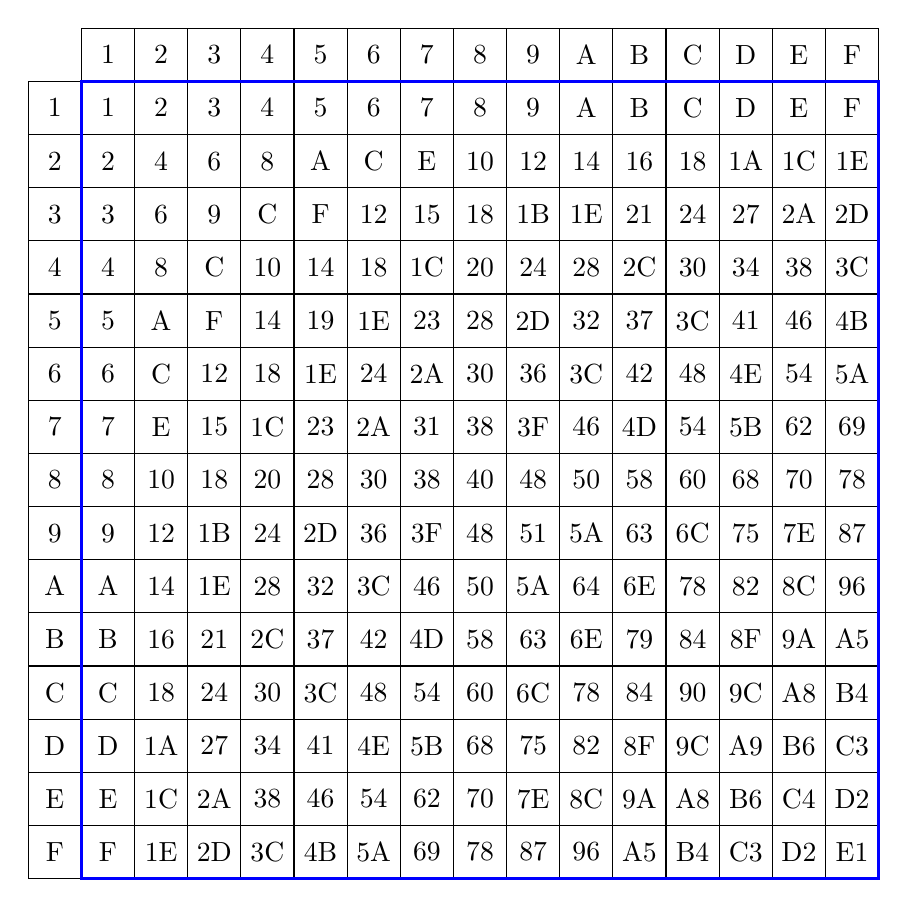
\begin{tikzpicture}[scale=0.675]
		% grid definition
		\draw (-1,0) grid (15,15);
		\draw (0,10) grid (15,16);
		\draw[line width=1pt, color=blue] (0,0) rectangle (15,15);
		
		% fill numbers
		\foreach \x in {1,2,3,...,15}
		\foreach \y in {1,2,3,...,15}
		\draw[shift={(-.5,-.5)}] (\x ,\y) node {\pgfmathHex{\number\numexpr\x*(16-\y)}\pgfmathresult\relax};
		
		% fill first row
		\foreach \x in {1,2,3,...,15}
		\draw[shift={(-.5,-.5)}] (\x , 16) node {\pgfmathHex{\x}\pgfmathresult};
		
		% fill first column
		\foreach \y in {1,2,3,...,15}
		\draw[shift={(-.5,-.5)}] (0, 16-\y) node {\pgfmathHex{\y}\pgfmathresult};
	\end{tikzpicture}
	\caption{Tavola Prodotti esadecimale}
	\label{tab:TavolaPitagoricaesadecimale}
\end{table}
\begin{table}[H]
	\centering
	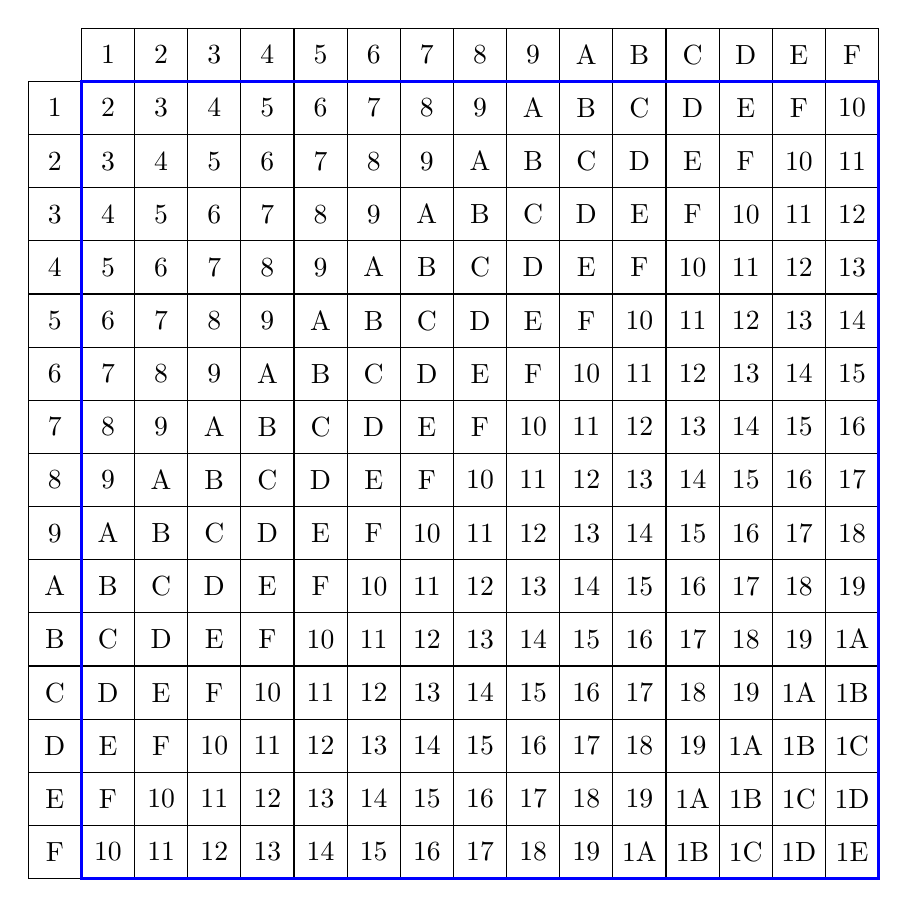
\begin{tikzpicture}[scale=0.675]
		% grid definition
		\draw (-1,0) grid (15,15);
		\draw (0,10) grid (15,16);
		\draw[line width=1pt, color=blue] (0,0) rectangle (15,15);
		
		% fill numbers
		\foreach \x in {1,2,3,...,15}
		\foreach \y in {1,2,3,...,15}
		\draw[shift={(-.5,-.5)}] (\x ,\y) node {\pgfmathHex{\number\numexpr\x+(16-\y)}\pgfmathresult\relax};
		
		% fill first row
		\foreach \x in {1,2,3,...,15}
		\draw[shift={(-.5,-.5)}] (\x , 16) node {\pgfmathHex{\x}\pgfmathresult};
		
		% fill first column
		\foreach \y in {1,2,3,...,15}
		\draw[shift={(-.5,-.5)}] (0, 16-\y) node {\pgfmathHex{\y}\pgfmathresult};
	\end{tikzpicture}
	\caption{Tavola somma esadecimale}
	\label{tab:Tavolaaddizioniesadecimale}
\end{table}
\subsection{Base otto}
\subsubsection{Conversioni}



\begin{table}[H]
	\centering
	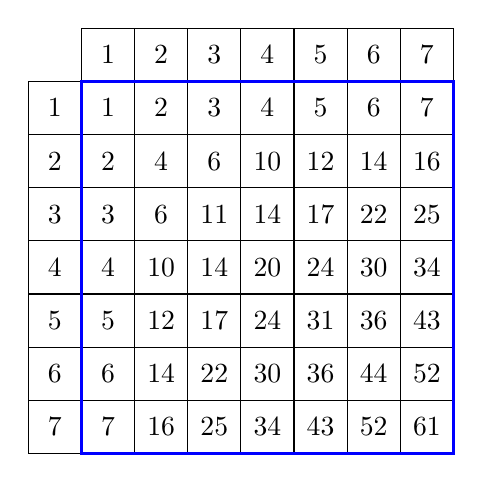
\begin{tikzpicture}[scale=0.675]
		% grid definition
		\draw (-1,0) grid (7,7);
		\draw (0,7) grid (7,8);
		\draw[line width=1pt, color=blue] (0,0) rectangle (7,7);
		
		% fill numbers
		\foreach \x in {1,2,3,...,7}
		\foreach \y in {1,2,3,...,7}
		\draw[shift={(-.5,-.5)}] (\x ,\y) node { \pgfmathoct{\number\numexpr\x*(8-\y)}\pgfmathresult\relax};
		
		% fill first row
		\foreach \x in {1,2,3,...,7}
		\draw[shift={(-.5,-.5)}] (\x , 8) node {\pgfmathoct{\x}\pgfmathresult};
		
		% fill first column
		\foreach \y in {1,2,3,...,7}
		\draw[shift={(-.5,-.5)}] (0, 8-\y) node {\pgfmathoct{\y}\pgfmathresult};
	\end{tikzpicture}
	\caption{Tavola Pitagorica ottale}
	\label{tab:TavolaPitagoricaottale}
\end{table}
\begin{table}[H]
	\centering
	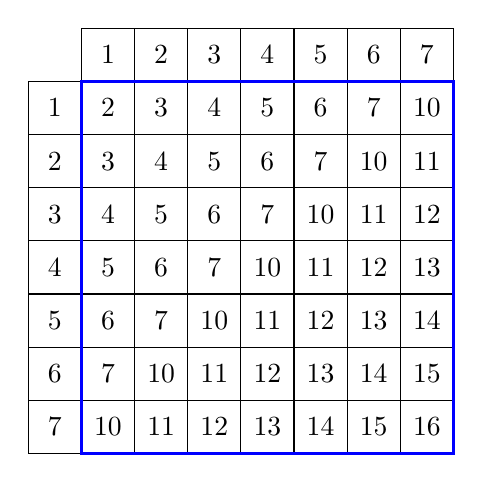
\begin{tikzpicture}[scale=0.675]
		% grid definition
		\draw (-1,0) grid (7,7);
		\draw (0,7) grid (7,8);
		\draw[line width=1pt, color=blue] (0,0) rectangle (7,7);
		
		% fill numbers
		\foreach \x in {1,2,3,...,7}
		\foreach \y in {1,2,3,...,7}
		\draw[shift={(-.5,-.5)}] (\x ,\y) node { \pgfmathoct{\number\numexpr\x+(8-\y)}\pgfmathresult\relax};
		
		% fill first row
		\foreach \x in {1,2,3,...,7}
		\draw[shift={(-.5,-.5)}] (\x , 8) node {\pgfmathoct{\x}\pgfmathresult};
		
		% fill first column
		\foreach \y in {1,2,3,...,7}
		\draw[shift={(-.5,-.5)}] (0, 8-\y) node {\pgfmathoct{\y}\pgfmathresult};
	\end{tikzpicture}
	\caption{Tavola Somma ottale}
	\label{tab:Tavolasommaottale}
\end{table}

	\chapter{Codifica Braille}
\label{Cha:CodificaBraille}
\begin{table}[H]
\begin{tabular}{cccc}
				\mytable{
					\braille{a} & a 1 \\
					\braille{b} & b 2 \\
					\braille{c} & c 3 \\
					\braille{d} & d 4 \\
					\braille{e} & e 5 \\
					\braille{f} & f 6 \\
					\braille{g} & g 7 \\
					\braille{h} & h 8 \\
					\braille{i} & i 9 \\
					\braille{j} & j 0 \\
					\braille{k} & k \\
					\braille{l} & l \\
					\braille{m} & m \\
					\braille{n} & n \\
					\braille{o} & o \\
				}&
				\mytable{
					\braille{p} & p \\
					\braille{q} & q \\
					\braille{r} & r \\
					\braille{s} & s \\
					\braille{t} & t \\
					\braille{u} & u \\
					\braille{v} & v \\
					\braille{w} & w \\
					\braille{x} & x \\
					\braille{y} & y \\
					\braille{z} & z \\
				}  &
				\mytable{
					\braille{{Capital}} & \{Maiuscolo\}\\
					\braille{{Upper}} & \{In alto\} \\
					%\braille{{Italic}} & \{Italic\} \\
				}
				&
				\mytable{
					\braille{{Number}} & \{Numero\} \\	
					\braille{{Letter}} & \{Lettera\} \\
				}   \\ 
				

			\end{tabular}
\caption[Codifica Braille]{ Codifica Braille (\copyright 1998-2010 William Park Licenza LPPL)}\label{tsd:}
\label{tab:CodificaBraille}
\end{table}
					
					
Ciao Mondo
					\braille{Ciao Mondo}
					
					1980
					\braille{{Number}1980}
	\chapter{Codifica ASCII}
\label{Cha:CodificaASCII}
	\settowidth{\gnat}{NUL}
	\settowidth{\gnam}{b1}
\begin{table}[H]

%	\begin{tabular}{r@{\hspace{0mm}}l}
%		& 
%		
%		\begin{tabular}{|N{\gnam}|*8{N{\gnat}}|}
%			\hline
%			$b_7$	& 0 & 0 & 0 & 0 & 1 & 1 & 1 & 1 \tabularnewline
%			
%			$b_6$	& 0 & 0 & 1 & 1 & 0 & 0 & 1 & 1 \tabularnewline
%			$b_5$	& 0 & 1 & 0 & 1 & 0 & 1 & 0 & 1 \tabularnewline
%			\hline
%		\end{tabular} 
%		\tabularnewline	
%		\begin{tabular}{|N{\gnam}|*4{N{\gnam}}}
%			\hline
%			$h_0$& $b_3$ &  $b_2$& $b_1$ & $b_0$ \tabularnewline 
%			\hline
%			0	& 0 & 0 & 0 & 0 \tabularnewline
%			1	& 0 & 0 & 0 & 1 \tabularnewline
%			2	& 0 & 0 & 1 & 0 \tabularnewline
%			3	& 0 & 0 & 1 & 1 \tabularnewline
%			4	& 0 & 1 & 0 & 0 \tabularnewline
%			5	& 0 & 1 & 0 & 1 \tabularnewline
%			6	& 0 & 1 & 1 & 0 \tabularnewline
%			7	& 0 & 1 & 1 & 1 \tabularnewline
%			8	& 1 & 0 & 0 & 0 \tabularnewline
%			9	& 1 & 0 & 0 & 1 \tabularnewline
%			A	& 1 & 0 & 1 & 0 \tabularnewline
%			B	& 1 & 0 & 1 & 1 \tabularnewline
%			C	& 1 & 1 & 0 & 0 \tabularnewline
%			D	& 1 & 1 & 0 & 1 \tabularnewline
%			E	& 1 & 1 & 1 & 0 \tabularnewline
%			F	& 1 & 1 & 1 & 1 \tabularnewline
%			\hline
%		\end{tabular} 
%		&
%		\begin{tabular}{|N{\gnam}|*8{N{\gnat}}|}
%			& 0 & 1 & 2 &  3& 4 & 5 & 6 & 7 \tabularnewline
%			\hline
%			0	& NUL & DLE & SP & 0 & @ & P & ` & p \tabularnewline
%			1	& SOH & DC1 & !  & 1 & A & Q & a & q \tabularnewline
%			2	& STX & DC2 & "  & 2 & B & R & b & r \tabularnewline
%			3	& ETX & DC3 & \# & 3 & C & S & c & s \tabularnewline
%			4	& EOT & DC4 & \$ & 4 & D & T & d & t \tabularnewline
%			5	& ENO & NAK & \% & 5 & E & U & e & u \tabularnewline
%			6	& ACK & SYN & \& & 6 & F & V & f & v \tabularnewline
%			7	& BEL & ETB & '  & 7 & G & W & g & w \tabularnewline
%			8	& BS  & CAN &  ( & 8 & H & X & h & x \tabularnewline
%			9	& HT  & EM  &  ) & 9 & I & Y & i & y \tabularnewline
%			10	& LF  & SUB & *  & : & J & Z & j & z \tabularnewline
%			11	& VT  & ESC & +  & ; & K & [  & k & \{ \tabularnewline
%			12	& FF  & FS  & ,  & < & L & \textbackslash & l & | \tabularnewline
%			13	& CR  & GS  & -  & = & M & ] & m & \} \tabularnewline
%			14	& SO  & RS  & .  & > & N & \^{}& n & \~{} \tabularnewline
%			15	& SI  & US  &  / & ? & O & \_ & o & DEL \tabularnewline
%			\hline
%		\end{tabular} 
%		\tabularnewline
%	\end{tabular}
\begin{tabular}{|M{\gnam}|*4{M{\gnam}}|M{\gnam}|*8{M{\gnat}}|}
	\cline{6-14}
	\multicolumn5{c|}{\pilH}	&$b_7$	& 0 & 0 & 0 & 0 & 1 & 1 & 1 & 1 \tabularnewline
	\multicolumn5{c|}{}		&$b_6$	& 0 & 0 & 1 & 1 & 0 & 0 & 1 & 1 \tabularnewline
	\multicolumn5{c|}{\pilD}	&$b_5$	& 0 & 1 & 0 & 1 & 0 & 1 & 0 & 1 \tabularnewline
	\hline
	$h_0$& $b_3$ &  $b_2$& $b_1$ & $b_0$ && 0 & 1 & 2 &  3& 4 & 5 & 6 & 7\pilH\pilD\tabularnewline
	\hline
	0	& 0 & 0 & 0 & 0 & 0	& NUL & DLE & SP & 0 & @ & P & ` & p\pilH\tabularnewline
	1	& 0 & 0 & 0 & 1 & 1	& SOH & DC1 & !  & 1 & A & Q & a & q \tabularnewline
	2	& 0 & 0 & 1 & 0 & 2	& STX & DC2 & \string"  & 2 & B & R & b & r \tabularnewline
	3	& 0 & 0 & 1 & 1 & 3	& ETX & DC3 & \# & 3 & C & S & c & s \tabularnewline
	4	& 0 & 1 & 0 & 0 & 4	& EOT & DC4 & \$ & 4 & D & T & d & t \tabularnewline
	5	& 0 & 1 & 0 & 1 & 5	& ENO & NAK & \% & 5 & E & U & e & u \tabularnewline
	6	& 0 & 1 & 1 & 0 & 6	& ACK & SYN & \& & 6 & F & V & f & v \tabularnewline
	7	& 0 & 1 & 1 & 1 & 7	& BEL & ETB & '  & 7 & G & W & g & w \tabularnewline
	8	& 1 & 0 & 0 & 0 & 8	& BS  & CAN &  ( & 8 & H & X & h & x \tabularnewline
	9	& 1 & 0 & 0 & 1 & 9	& HT  & EM  &  ) & 9 & I & Y & i & y \tabularnewline
	A	& 1 & 0 & 1 & 0 & 10& LF  & SUB & *  & : & J & Z & j & z \tabularnewline
	B	& 1 & 0 & 1 & 1 & 11& VT  & ESC & +  & ; & K & [  & k & \{ \tabularnewline
	C	& 1 & 1 & 0 & 0 & 12& FF  & FS  & ,  & < & L & \textbackslash & l & | \tabularnewline
	D	& 1 & 1 & 0 & 1 & 13& CR  & GS  & -  & = & M & ] & m & \} \tabularnewline
	E	& 1 & 1 & 1 & 0 & 14& SO  & RS  & .  & > & N & \textasciicircum& n & \textasciitilde \tabularnewline
	F	& 1 & 1 & 1 & 1 & 15& SI  & US  &  / & ? & O & \_ & o & DEL\rule[-1.5ex]{0pt}{0pt}\tabularnewline
	\hline
\end{tabular}
	\caption{Codifica ASCII}
\end{table}
	\chapter{Algebra di Boole}
\label{cha:AlgebradiBoole}
%\FloatBarrier
\section{Variabili e funzioni booleane}
\label{sec:VariabiliBooleane}
Una variabile booleana\index{Variabile!booleana} è una variabile che può assumere solo due valori, che possono essere indicati o  con\nobs$0$\nobs e\nobs$1$ o con $basso$\nobs e\nobs$alto$, con $vero$\nobs o \nobs$falso$. Nella realtà, a questi valori sono  associati valori arbitrari es: $+5\si{\volt}$ $-5\si{\volt}$, $+12\si{\volt}$ $-12\si{\volt}$. 

 Un sistema si trova in un determinato stato a seconda del valore che assumono le variabili booleane associate.   Vi sono due variabili  particolari la variabile\nobs$0$ che assume solo il valore\nobs$0$ e la variabile \nobs$1$ che assume solo il valore\nobs$1$. 

Una funzione (operazione) booleana\index{Funzione!booleana} è una relazione  che ha in ingresso delle variabili indipendenti e in uscita una variabile dipendente.

A ogni sistema è associata una tabella detta tavola di verità\index{Tavola di verità}. Una tavola di verità rappresenta in forma tabellare, in base agli stati del sistema in entrata, lo stato del sistema in uscita. Si può facilmente provare %, utilizzando la tavola~\vref{tab:statisistema},  
che la tabella\vref{tab:totfunzzionilogiche} rappresenta tutte le funzioni logiche con due valori in entrata.

Due funzioni logiche sono equivalenti\index{Funzione!booleana!equivalente} se hanno la stessa tavola di verità. Esempio di questo sono la tabella\nobs\vref{tab:tabVeritaEOR} e la tabella\nobs\vref{tab:tabVeritaEOR2} che sono fra di loro equivalenti. 

Un metodo grafico per rappresentare una funzione logica  è il circuito che si ottiene combinando i simboli  elencati nella tabella\nobs\vref{tab:Portelogichetavver}. Un esempio di ciò sono  i due circuiti\nobs\vref{Tab:circuito2e3} che rappresentano entrambi la funzione $XOR$\index{Funzione!booleana!XOR}  ottenuta come combinazione di $AND$\index{Funzione!booleana!AND} e $OR$\index{Funzione!booleana!OR}

Principio di dualità: Se una funzione logica è vera, allora è vera la funzione che si ottiene scambiando $AND$ con  $OR$ e  $0$ con $1$ e viceversa.

\begin{table} %[H]
	%\centering
	\begin{tabular}{cccccccccccccccccc}
	\toprule
	A & B & $0$ & NOR & $\overline{A}$ &  &  & $\overline{B}$ & XOR & NAND & AND & XNOR &  & B & A &  & OR & $1$ \\ 
	\midrule
	1 & 1 & 0 & 0 & 0 & 0 & 0 & 0 & 0 & 0 & 1 & 1 & 1 & 1 & 1 & 1 & 1 & 1 \\ 
	1 & 0 & 0 & 0 & 0 & 0 & 1 & 1 & 1 & 1 & 0 & 0 & 0 & 0 & 1 & 1 & 1 & 1 \\ 
	0 & 1 & 0 & 0 & 1 & 1 & 0 & 0 & 1 & 1 & 0 & 0 & 1 & 1 & 0 & 0 & 1 & 1 \\ 
	0 & 0 & 0 & 1 & 1 & 0 & 0 & 1 & 0 & 1 & 0 & 1 & 1 & 0 & 0 & 1 & 0 & 1 \\ 
	\bottomrule
	\end{tabular}
	\caption{Funzioni logiche}
	\label{tab:totfunzzionilogiche}
\end{table}
\subsection{Esempi}
\label{sec:Esempiofunzlog}
Definire, utilizzando le funzioni logiche:

$tavolo=(legno,ferro,3gambe,4gambe,piano)$,

$auto=(3 porte,5 porte,ruote,motore)$, 

$penna=(sfera,stilografica,rossa,nera,verde,cancellabile,indelebile)$

Una cassaforte ha quattro lucchetti, x, y, v, w, che devono essere tutti aperti affinché la
cassaforte si apra.  Tre persone A, B, C,  hanno le  chiavi. A possiede le chiavi v e y; 
B ha le chiavi v e x e C tiene w e y. Le variabili A, B, C sono uguali a uno se la persona corrispondente è presente, altrimenti sono uguali a zero. Costruire la tavola
della verità della funzione $Y=f(A,B,C)$. La funzione  vale uno se e solo se la cassaforte può essere  aperta,
 esprimere f in forma algebrica. Per risolvere almeno la prima parte dell'esercizio costruiamo una tabella  che leghi le chiavi alle tre persone.
\begin{table}
	    \centering
		\begin{tabular}{c|cccc}
			& \textbf{x} & \textbf{y} &\textbf{v}& \textbf{w}\\
			\toprule 
			\textbf{A} &  & \textbullet &\textbullet & \\ 
			\textbf{B} & \textbullet &  & \textbullet& \\ 
			\textbf{C} &  & \textbullet & & \textbullet\\ 
			\bottomrule
		\end{tabular}
	\caption[]{Persone e chiavi}
	\label{tab:personeechiavi}
\end{table} 
Quindi: il sistema (la cassaforte aperta o chiusa), dipende da tre variabili $A$, $B$ e $C$ che assumono solo due valori $1$ se la chiave è presente o $0$ altrimenti. In uscita $Y$ può assumere due valori $1$ se la cassaforte è aperta o $0$ nell'altro caso. 

La tabella~\vref{tab:personeechiavi} permette di costruire la tavola di verità\nobs\vref{tab:tavolaveritacasaforte} della funzione. La tabella, dipendendo da tre variabili in ingresso, ha otto stati. Iniziamo a costruire la tavola di verità del sistema. Nella prima riga abbiamo che $A=0$, $B=0$ e $C=0$, poiché nessuna chiave è presente, la cassaforte rimane chiusa quindi $Y=0$. Nella seconda riga abbiamo che $A=0$, $B=0$ e $C=1$,  due chiavi sono presenti ma \nobs\vref{tab:personeechiavi} ci dice che queste non bastano e la cassaforte è chiusa e quindi $Y=0$. Il discorso è analogo  per le righe rimanenti. Nella riga quattro abbiamo che $A=0$, $B=1$ e $C=1$  sono presenti quattro chiavi e la cassaforte viene aperta per cui $Y=1$.  Stesso discorso la riga otto e anche in questo caso $Y=1$.
\begin{table}
		\centering
\begin{tabular}{c|c|c|c|c}
	& \textbf{A} & \textbf{B} & \textbf{C} & \textbf{Y} \\
	\toprule 
	1& 0 & 0 & 0 & 0 \\ 
	2& 0 & 0 & 1 &  0\\ 
	3& 0 & 1 & 0 &  0\\ 
	4& 0 & 1 & 1 &  1\\ 
	5& 1 & 0 & 0 &  0\\ 
	6& 1 & 0 & 1 &  0\\ 
	7& 1 & 1 & 0 &  0\\ 
	8& 1 & 1 & 1 &  1\\ 
	\bottomrule
\end{tabular} 
	\caption{Tavola di verità}
	\label{tab:tavolaveritacasaforte}
\end{table}
\section{Tavole di verità}
\label{sec:TavoleDiVeritA}
\begin{figure} %[H]
\centering
	\pagestyle{empty}
	% Set the overall layout of the tree
\tikzstyle{level 1}=[level distance=3.5cm, sibling distance=3.5cm]
\tikzstyle{level 2}=[level distance=3.5cm, sibling distance=2cm]
\tikzstyle{level 3}=[level distance=3cm, sibling distance=0.8cm] 
% Define styles for bags and leafs
%\tikzstyle{bag} = [text width=4em, text centered]
\tikzstyle{bag} =[shape=circle,draw,
text centered]
\begin{tikzpicture}[grow=right, sloped]
\matrix [row sep=1em] 
{
	\node[bag] {0}
	child{   
		node[bag] {0}
		child{
			node[bag] {0}
			child{
				node[bag]{0}
			}
			child{
				node[bag]{1}
			}
		}
		child {
			node[bag] {1}
			child{
				node[bag]{0}
			}
			child{
				node[bag]{1}
			}		
		}
	}
	child{
		node[bag]{1}
		child{
			node[bag] {0}
			child{
				node[bag]{0}
			}
			child{
				node[bag]{1}
			}
		}
		child {
			node[bag] {1}
			child{
				node[bag]{0}
			}
			child{
				node[bag]{1}
			}
		}   
	};
	&\\
	\draw (0,0) --  (10.5,0);
	\draw (0.0,1pt) -- (0.0,-3pt)
	node[anchor=north] {1};
	\draw (3.5,1pt) -- (3.5,-3pt)
	node[anchor=north] {2};
	\draw (7,1pt) -- (7,-3pt)
	node[anchor=north] {3};
	\draw (10,1pt) -- (10,-3pt)
	node[anchor=north] {4};\\
	\node[bag] {0}
	child{   
		node[bag] {0}
		child{
			node[bag] {0}
			child{
				node[bag]{0}
			}
			child{
				node[bag]{1}
			}
		}
		child {
			node[bag] {1}
			child{
				node[bag]{0}
			}
			child{
				node[bag]{1}
			}		
		}
	}
	child{
		node[bag]{1}
		child{
			node[bag] {0}
			child{
				node[bag]{0}
			}
			child{
				node[bag]{1}
			}
		}
		child {
			node[bag] {1}
			child{
				node[bag]{0}
			}
			child{
				node[bag]{1}
			}
		}   
	};\\
};
\end{tikzpicture}
	\caption{Stati del sistema}
	\label{tab:statisistema}
\end{figure}

Le funzioni logiche sono divise in gruppi. Il primo è formato dalle funzioni AND\index{Funzione!booleana!AND}, OR\index{Funzione!booleana!OR} e NOT\index{Funzione!booleana!NOT}. Segue il gruppo formato solo da NAND\index{Funzione!booleana!NAND}. Infine quello composto solo  da NOR\index{Funzione!booleana!NOR}. Ogni gruppo è tale perché in grado di generare le rimanenti funzioni. La figura~\vref{tab:Portelogichetavver} riporta le tavole di verità di queste funzioni. 

Combinando fra di loro le funzioni  otteniamo altre funzioni come viene per esempio, nella tabella~\vref{tab:ComposizionePorte}. 

La tabella~\vref{tab:statisistema} da in verticale di quante righe deve avere una tavola di verità.  Con una variabile due righe,  due variabili  otteniamo quattro righe etc. Mentre in orizzontale,in base al numero delle variabili, percorrendo i grafi da sinistra verso destra, avremo tutti i possibili stati di un sistema.
\subsection{Funzione AND}
\label{sub:funzioneAND}
La funzione AND\index{Funzione!booleana!AND} ha due valori in entrata ed  un valore in uscita che è vero solo quando sono veri entrambi i valori in entrata. Il simbolo che la rappresenta l'operazione è il prodotto.

Nella realtà casi in cui si usano funzioni AND sono molteplici. In genere si usa una funzione AND\index{Funzione!booleana!AND} quando  si eseguono due azioni in contemporaneamente come per esempio nel dispositivi di azionamento di una pressa in cui si premono contemporaneamente due pulsanti in modo da impegnare entrambe le mani, evitando così incidenti. 

Un esempio della funzione AND\index{Funzione!booleana!AND} è il seguente circuito\nobs\vref{tab:elettricoAND}. Abbiamo un circuito con due pulsanti in serie.  La lampada si accende solo premendo solo contemporaneamente i due interruttori.
\begin{table}[H]
	\centering
	\begin{circuitikz} \draw
		(0,0)--(0,2)
		(5,0)--(5,2)
		(0,0) to[lamp] (2,0)
		(2,0) to[battery] (5,0)
		(0,2) to[opening switch] (3,2)
		(3,2) to[opening switch] (5,2);
	\end{circuitikz}
	\caption{Circuito AND}
	\label{tab:elettricoAND}
\end{table}
	
La tabella\nobs\ref{tab:Portelogichetavver} mostra la tavola di verità\index{Tavola di verità!AND} della $AND$\index{Funzione!booleana!AND} e il simbolo grafico associato.
\subsection{Funzione OR}
\label{sub:funzioneOR}
La funzione OR\index{Funzione!booleana!OR} ha due valori in entrata e un valore in uscita. Questo valore è vero quando almeno uno dei valori in ingresso è vero. Il simbolo che la rappresenta è la somma. 

Un esempio dell'uso della funzione OR\index{Funzione!booleana!OR} è l'impianto di illuminazione di una stanza in cui due interruttori distinti permettono di accendere una lampadina.

Un circuito in parallelo, come il circuito\nobs\vref{tab:ZunzioneOR}, rappresenta la funzione OR\index{Funzione!booleana!OR}. Per accendere la lampadina basta premere almeno un interruttore.
\begin{table}
	\centering
	\begin{circuitikz} \draw
		(0,0)--(0,2)
		(5,0)--(5,2)
		(0,0) to[lamp] (2,0)
		(2,0) to[battery] (5,0)
		(0,2)--(1,2)
		(1,1)--(1,3)
		(4,1)--(4,3)
		(4,2)--(5,2)
		(1,3) to[opening switch] (4,3)
		(1,1) to[opening switch] (4,1);
	\end{circuitikz}
	\caption{Circuito OR}
	\label{tab:ZunzioneOR}
\end{table}
La tabella\nobs\ref{tab:Portelogichetavver} mostra la tavola di verità\index{Tavola di verità!OR} della OR\index{Funzione!booleana!OR} e il simbolo grafico associato.
\subsection{Funzione NOT}
\label{sub:funzionenot}
La funzione NOT ha un solo valore in entrata e un solo valore in uscita. Il valore in uscita è l'opposto a quello in ingresso. Il simbolo che rappresenta l'operazione è un trattino che si pone sopra la variabile.

Un esempio dell'uso della funzione NOT\index{Funzione!booleana!NOT} è per esempio l'interruttore della luce di cortesia di un'auto che si accende aprendo la portiera.

Un circuito come il circuito\nobs\vref{tab:CircuitoNOT} rappresenta la funzione NOT. La tabella\nobs\ref{tab:Portelogichetavver} mostra la tavola di verità\index{Tavola di verità!NOT} della NOT e il simbolo grafico associato.
\begin{table}
	\centering
	 \begin{circuitikz} \draw
		(0,0)--(0,2)
		(6,0)--(6,2)
		(0,1) to[lamp] (6,1)
		(0,2)--(3,2)
		(3,2) to[battery,v_<=$+-$] (6,2)
		(0,0) to[opening switch] (3,0)
		(3,0) to[battery,v_<=$+-$] (6,0);
	\end{circuitikz}
	\caption{Circuito NOT}
	\label{tab:CircuitoNOT}
\end{table}
	
\subsection{Funzione XOR}
\label{sub:funzioneXOR}
La funzione XOR\index{Funzione!booleana!XOR} ha due valori in entrata ed un valore in uscita che è vero quando solo uno dei valori in ingresso è vero.

Il circuito\nobs\vref{tab:circuitoXOR} rappresenta un OR esclusivo. Sono due gruppi di pulsanti in parallelo messe in serie. La seconda serie di pulsanti sono i negati dei precedenti. Quando vien premuto il primo pulsante $A$ il pulsante $\overline{A}$ del secondo circuito viene aperto e viceversa, analogamente per il pulsante $B$. In questo circuito la corrente passa e  lampadina si accende, solo se è premuto un solo pulsante ma non entrambi.

La tabella\nobs\ref{tab:Portelogichetavver} mostra la tavola di verità della XOR\index{Tavola di verità!XOR} e il simbolo grafico associato.
\begin{table} %[H]
		\centering
		\begin{circuitikz} \draw
			(0,0)--(0,2)
			(7,0)--(7,2)
			(0,0) to[lamp] (3,0)
			(3,0) to[battery] (7,0)
			(0,2)--(1,2)
			(1,1)--(1,3)
			(3,1)--(3,3)
			(3,2)--(4,2)
			(4,1)--(4,3)
			(6,1)--(6,3)
			(6,2)--(7,2)
			(1,3) to[opening switch=$A$] (3,3)
			(1,1) to[opening switch=$B$] (3,1)
			(4,1) to[closing switch=$\overline{B}$] (6,1)
			(4,3) to[closing switch=$\overline{A}$] (6,3);
		\end{circuitikz}
	\caption{Circuito XOR}
	\label{tab:circuitoXOR}
	\end{table}
\subsection{Funzione NAND}
\label{sub:funzioneNAND}
La funzione NAND\index{Funzione!booleana!NAND} ha due valori in entrata ed ha un valore in uscita che è falso solo quando sono veri entrambi i valori in entrata.

La tabella\nobs\ref{tab:Portelogichetavver} mostra la tavola di verità\index{Tavola di verità!NAND} della $NAND$\index{Funzione!booleana!NAND} e il simbolo grafico associato. La $NAND$ è la negazione di $AND$\index{Funzione!booleana!AND}.

\subsection{Funzione NOR}
\label{sub:funzioneNOR}
La funzione NOR\index{Funzione!booleana!NOR} ha due valori in entrata ed ha un valore in uscita che è vero solo quando sono falsi entrambi i valori in entrata.

La tabella\nobs\ref{tab:Portelogichetavver} mostra la tavola di verità\index{Tavola di verità!NOR} della NOR\index{Funzione!booleana!NOR} e il simbolo grafico associato. La NOR è la negazione di OR 
\subsection{Funzione XNOR}
\label{sub:funzioneXNOR}
La funzione XNOR\index{Funzione!booleana!XNOR} ha due valori in entrata ed ha un valore in uscita che è vero solo quando sono falsi entrambi i valori in entrata o quando sono entrambi veri. 

La tabella\nobs\ref{tab:Portelogichetavver} mostra la tavola di verità\index{Tavola di verità!XNOR} della XNOR e il simbolo grafico associato. La XNOR è la negazione di XOR 

Il circuito\nobs\vref{tab:circuitoXNOR} è formato da due blocchi di pulsanti in serie messi in parallelo. Quando vien premuto il primo pulsante $A$ il pulsante $\overline{A}$ del secondo circuito viene aperto e viceversa, analogamente per il pulsante $B$. La lampadina si accende o quando entrambi i pulsanti $A$ e $B$ sono premuti o entrambi i  pulsanti $A$ e $B$ sono tenuti alzati.
\begin{table}[H]
	\centering
	\begin{circuitikz} \draw
		(0,0)--(0,2)
		(7,0)--(7,2)
		(0,0) to[lamp] (3,0)
		(3,0) to[battery] (7,0)
		(0,2)--(1,2)
		(1,1)--(1,3)
		(6,1)--(6,3)
		(6,2)--(7,2)
		(1,3) to[opening switch=$A$] (4,3)
		(4,3) to[opening switch=$B$] (6,3)
		(1,1) to[closing switch=$\overline{A}$] (4,1)
		(4,1) to[closing switch=$\overline{B}$] (6,1);
	\end{circuitikz}
	\caption{Circuito XNOR}
	\label{tab:circuitoXNOR}
\end{table}
Come si è detto a una funzione logica è possibile associare una tavola di verità\index{Tavola di verità!Costruire}. Un esempio di costruzione  è la tabella~\vref{tab:tabVeritaEOR}. Il metodo usato è molto semplice,  prevede di suddividere la funzione nelle sue componenti e risolverle partendo da sinistra verso destra. Questo deve essere fatto rispettando le convenzioni di precedenza, cioè le negazioni (funzione NOT), poi i prodotti (Funzione AND\index{Funzione!booleana!AND}), e infine le somme (Funzione OR\index{Funzione!booleana!OR}).Possiamo cambiare le  precedenze mettendo fra  delle parentesi le operazioni che devono essere eseguite prima.
In conclusione, abbiamo parlato di tavola di verità\index{Tavola di verità}, circuito, funzione logica, che sono concetti fra loro equivalenti\vref{tab:FunzioneTavolaCircuito} e fra loro connessi.
\begin{table} 
	\centering
	\begin{tikzpicture}[very thick,node distance=5cm,text centered,minimum size=3cm]
		\node [circle, draw] (a) {Funzione logica};
		\node [circle, draw] (b) [above right=of a] {Tavola di verità};
		\node [circle, draw] (c) [above left=of a]{Circuito};
		\draw [<->] (a) to (b);
		\draw [<->] (b) to (c);
		\draw [<->] (c) to (a);
	\end{tikzpicture}
	\caption{Funzione, Tavola e Circuito}
	\label{tab:FunzioneTavolaCircuito}
\end{table}
\begin{table}
	\centering
	\begin{tabular}{@{}cc@{\hspace{2cm}}cc@{}}
	\begin{truthtable}{AND}
	\toprule
	$A$&$B$&$AB$\\
	\midrule           
	0&0&0\\
	1&0&0\\
	0&1&0\\
	1&1&1\\
	\bottomrule
	\end{truthtable}
	& \cport{and} &
	\begin{truthtable}{NAND}
	\toprule
	$A$&$B$&$A\mathbin{\overline{\wedge}}B$\\
	\midrule
	0&0&1\\
	1&0&1\\
	0&1&1\\
	1&1&0\\
	\bottomrule
	\end{truthtable}
	& \cport{nand} \\
	\addlinespace[3ex]
	\begin{truthtable}{OR}
	\toprule
	$A$&$B$&$A+B$\\
	\midrule         
	0&0&0\\
	1&0&1\\
	0&1&1\\
	1&1&1\\
	\bottomrule
	\end{truthtable}
	& \cport{or} &
	\begin{truthtable}{NOR}
	\toprule
	$A$&$B$&$A\mathbin{\overline{\vee}}B$\\
	\midrule
	0&0&1\\
	1&0&0\\
	0&1&0\\
	1&1&0\\
	\bottomrule
	\end{truthtable}
	& \cport{nor} \\
	\addlinespace[3ex]
	\begin{truthtable}{XOR}
	\toprule
	$A$&$B$&$A\XOR B$\\
	\midrule         
	0&0&0\\
	1&0&1\\
	0&1&1\\
	1&1&0\\
	\bottomrule
	\end{truthtable}
	& \cport{xor} &
	\begin{truthtable}{XNOR}
	\toprule
	$A$&$B$&$A\mathbin{\overline{\XOR}}B$\\
	\midrule
	0&0&1\\
	1&0&0\\
	0&1&0\\
	1&1&1\\
	\bottomrule
	\end{truthtable}
	& \cport{xnor} \\
	\addlinespace[3ex]
	\multicolumn{4}{c}{%
		\begin{tabular}{@{}cc@{}}
		\begin{truthtable}[2]{NOT}
		\toprule
		$A$&$\overline{A}$\\
		\midrule         
		0&1\\
		1&0\\
		\bottomrule
		\end{truthtable}
		& \cport{not}
		\end{tabular}}
	\end{tabular}
	\caption{Porte logiche}
	\label{tab:Portelogichetavver}
\end{table} 
\begin{table} %[H]
	\centering
	\begin{tabular}{ccc}
	\toprule
	\begin{circuitikz} \draw
	(0,0) node[and port] (myand) {}
	(1,0) node[not port] (mynot) {}
	(myand.out) -- (mynot.in)
	;\end{circuitikz}&&\begin{circuitikz} \draw
	(0,0) node[nor port]  {}
	;\end{circuitikz} \\
	AND +  NOT &=&NAND \\
	\midrule
	\begin{circuitikz} \draw
	(0,0) node[or port] (myor) {}
	(1,0) node[not port] (mynot) {}
	(myor.out) -- (mynot.in)
	;\end{circuitikz}&& \begin{circuitikz} \draw
	(0,0) node[nor port]  {}
	;\end{circuitikz} \\
	OR +  NOT &=&NOR  \\ 
	\midrule
	\begin{circuitikz} \draw
	(0,0) node[xor port] (myxor) {}
	(1,0) node[not port] (mynot) {}
	(myxor.out) -- (mynot.in)
	;\end{circuitikz}&& \begin{circuitikz} \draw
	(0,0) node[xnor port]  {}
	;\end{circuitikz} \\
	XOR +  NOT &=&XNOR  \\ 
	\bottomrule
	\end{tabular} 
	\caption{Composizione porte}%
	\label{tab:ComposizionePorte}%
\end{table}
\section{Proprietà dell'algebra algebra booleana}
\label{sec:Algebrabooleana}
La tabella\nobs\vref{Tab:AlgebrAbOOLEAN} elenca le principali proprietà delle funzioni AND\index{Funzione!booleana!AND} e OR\index{Funzione!booleana!OR} e mostra come le proprietà delle funzioni siano legate tramite il principio di dualità. Infatti, osservando la tabella si vede come le proprietà elencate a sinistra trovino il loro corrispondente duale a destra e viceversa. La tabella\nobs\vref{Tab:funzlogSemp} mostra come ottenere i risultati. Non vengono dimostrate tutte le relazioni inquarto le altre si ottengono per dualità.

%\altapriorita{Specificare meglio}
Una funzione logica non è unica ma può essere scritta in modi fra di loro equivalenti. La tabella\nobs\vref{Tab:funzlogSemp} mostra come con pochi passaggi si può passare da una funzione logica a una equivalente.
\begin{table}%[H]
\centering
\begin{tabular}{lcl}
\toprule
&PROPRIET\'A&\\
&$\overline{\overline{A}}=A$&\\
$A+0=A$&Elemento neutro&$A\cdot1=A$\\
$A+1=1$&Assorbimento&$A\cdot0=0$\\
$A+A=A$&Idempotenza&$A\cdot A=A$\\
$A+\overline{A}=1$&&$A\cdot\overline{A}=0$\\
$A+B=B+A$&Commutativa&$A\cdot B=B\cdot A$\\
$(A\cdot B)\cdot C=A\cdot(B\cdot C)=A\cdot B\cdot C$&Associativa&$(A+B)+C=A+(B+C)=A+B+C$\\
\midrule
&TEOREMI&\\
\midrule
$A+A\cdot B=A$&&$A\cdot(A+B)=A$\\
$A+\overline{A}\cdot B=A+B$&&$A\cdot (\overline{A}+B)=AB$\\
$(A+B)\cdot(A+C)=A+B\cdot C$&&$A\cdot B+A\cdot C=A\cdot(B+C)$\\
$(A+B)\cdot(\overline{A}+C)=\overline{A}\cdot B+A\cdot C$&&$A\cdot B+\overline{A}\cdot C=(\overline{A}+B)\cdot(A+B)$\\
\midrule
&TEOREMI DI DE MORGAN&\\
\midrule
$\overline{A+B}=\overline{A}\cdot\overline{B}$&&$\overline{A\cdot B}=\overline{A}+\overline{B}$\\
\bottomrule
\end{tabular}
\caption{Teoremi e proprietà algebra di Boole}%
\label{Tab:AlgebrAbOOLEAN}%
\end{table}
\begin{table}
\centering
\begin{tabular}{lcl}
\toprule
%\midrule
PROPRIET\'A&&DIMOSTRAZIONE\\
\midrule
$A+A\cdot B=A$&&$A+A\cdot B=$\\
&&$=A\cdot(1+B)=$\\
&&$=A\cdot1=A$\\ 
\midrule
$A+\overline{A}\cdot B=A+B$&&$A+A\cdot B+\overline{A}\cdot B=$\\
&&$=A+(A+\overline{A})\cdot B=$\\
&&$=A+1\cdot B=$\\
&&$=A+B$\\
\midrule
$(A+B)\cdot(A+C)=A+B\cdot C$&&$(A+B)\cdot(A+C)=$\\
&&$A\cdot A+A\cdot C+A\cdot B+B\cdot C=$\\
&&$=A+A\cdot C+A\cdot B+B\cdot C=$\\
&&$=A\cdot(1+C) +A\cdot B+B\cdot C=$\\
&&$=A\cdot 1 +A\cdot B+B\cdot C=$\\
&&$=A\cdot(1+B)+B\cdot C=$\\
&&$A+B\cdot C$\\
\midrule
$(A+B)\cdot(\overline{A}+C)=\overline{A}\cdot B+A\cdot C$&&$(A+B)\cdot(\overline{A}+C)$\\
&&$\overline{A}\cdot A+ A\cdot C +\overline{A}\cdot B+B\cdot A\cdot C$\\
&&$A\cdot B+\overline{A}\cdot B+B\cdot C$\\
&&$(A+B)\cdot C+\overline{A}\cdot B$\\
&&$(A+\overline{A}\cdot B)\cdot C+\overline{A}\cdot B$\\
&&$A\cdot C+\overline{A}\cdot B\cdot C+\overline{A}\cdot B$\\
&&$A\cdot C+\overline{A}\cdot B(C+1)$\\
&&$A\cdot C+\overline{A}\cdot B$\\
\bottomrule
\end{tabular}
\caption{Semplificazioni}
\label{Tab:funzlogSemp}
\end{table}
\section{Trovare la tavola di verità di una funzione}
\label{sec:Trovaretavolaveritàfunzione}
Per trovare data una funzione, la tavola di verità\index{Tavola di verità}, basta sostituire alle variabili booleane  i valori in ingresso e vedere cosa ha la funzione in uscita. 

Consideriamo la funzione $Y=A\cdot\overline{B}+\overline{A}\cdot B$  possiamo costruire la tabella\nobs\vref{tab:tabVeritaEOR} che fornisce tutti i calcoli necessari. Si procede sostituendo alle variabili tutti i valori possibili e ottenendo dopo i calcoli i risultati della colonna sette 

Analogo ragionamento è per $Y=(A+B)\cdot(\overline{A}+\overline{B})$ e ottenere la tabella\nobs\vref{tab:tabVeritaEOR2}.

Per $Y=\overline{A}\cdot\overline{B}\cdot C+\overline{A}\cdot B\cdot\overline{C}+\overline{A}\cdot B\cdot C+A\cdot B\cdot C$ otteniamo la tavola di verità\nobs\vref{Tab:esempio2bool}\index{Tavola di verità}

La tavola di verità per $Y=\overline{A}\cdot (A+B)+\overline{C}+B\cdot C$ e per $Y=B+\overline{C}$ è\nobs\vref{Tab:Tabveres1}
\begin{table}
	\centering
	\begin{tabular}{ccccccccccc}
		\toprule
		\multicolumn{10}{c}{$A\cdot\overline{B}+\overline{A}\cdot B$} \\ 
		&  &  & 1 & 3 & 2 & 7 & 4 & 6 & 5 \\ 
		A & B &  & $A$&$\cdot$  &$\overline{B}$&$+$& $\overline{A}$ &$\cdot$ &$B$  \\ 
		\cmidrule{1-2}\cmidrule{4-10}
		1 & 1 &  & 1 & 0 & 0 & 0 & 0 & 0 & 1 \\ 
		1 & 0 &  & 1 & 1 & 1 & 1 & 0 & 0 & 0 \\ 
		0 & 1 &  & 0 & 0 & 0 & 1 & 1 & 1 & 1 \\ 
		0 & 0 &  & 0 & 0 & 1 & 0 & 1 & 0 & 0 \\ 
		\bottomrule
	\end{tabular}
	\caption[]{Tavola di verità di $A\cdot\overline{B}+\overline{A}\cdot B$}
	\label{tab:tabVeritaEOR}
\end{table}
\begin{table}
	\centering
	\begin{tabular}{ccccccccccc}
		\toprule
		\multicolumn{10}{c}{$(A+B)\cdot(\overline{A}+\overline{B})$} \\ 
		&  &  & 1 & 3 & 2 & 7 & 4 & 6 & 5 \\ 
		A & B &  & $(A$&$+$  &$B)$ &$\cdot$ &$(\overline{A}$&$+$&$\overline{B})$  \\ 
		\cmidrule{1-2}\cmidrule{4-10}
		1 & 1 &  & 1 & 1 & 1 & 0 & 0 & 0 & 0 \\ 
		1 & 0 &  & 1 & 1 & 0 & 1 & 0 & 1 & 1 \\ 
		0 & 1 &  & 0 & 1 & 1 & 1 & 1 & 1 & 0 \\ 
		0 & 0 &  & 0 & 0 & 0 & 0 & 1 & 1 & 1 \\ 
		\bottomrule
	\end{tabular}
	\caption[]{Tavola di verità di $(A+B)\cdot(\overline{A}+\overline{B})$}
	\label{tab:tabVeritaEOR2}
\end{table}
\section{Trovare la funzione data la tavola di verità}
\label{sec:Trovarefunzionedatatavolaverità}
Per trovare la funzione, nota la tavola di verità\index{Tavola di verità!trovare!funzione}, possiamo utilizzare due metodi\footnote{I due metodi sono duali come si nota leggendo di seguito} 
\subsection{Somma di prodotti canonici} 
Per trovare data la tavola di verità la funzione si usa il metodo della somma di prodotti canonici\index{Somma prodotti canonici!\see{Mintermini}}. Ogni funzione logica si può scrivere come somma di prodotti detti mintermini\index{Mintermini}. Questi prodotti sono costituiti da prodotti di tutte le variabili in forma diretta o negata. Ogni mintermine assume il valore logico 1.

Nell'esempio uno si inizia dalla tavola\nobs\vref{Tab:esempio2bool},  si individuano le righe che hanno come risultato uno e si costruisce la somma dei mintermini. Nella riga due della tavola di verità si ha come risultato uno. Dato che le variabili $A$ $B$ assumono valore zero nel prodotto si inserisce il loro complemento e otteniamo $\overline{A}\cdot \overline{B}\cdot C$.

Si continua con lo stesso criterio ed otteniamo\[Y=2+3+4+8=\overline{A}\cdot\overline{B}\cdot C+\overline{A}\cdot B\cdot\overline{C}+\overline{A}\cdot B\cdot C+A\cdot B\cdot C\] cioè la funzione associata.
\begin{table}
	\centering
	\begin{tabular}{lccc|c}
		&A&B&C&Y\\
		\toprule
		1&0&0&0&0\\
		2&0&0&1&\textbf{1}\\
		3&0&1&0&\textbf{1}\\
		4&0&1&1&\textbf{1}\\
		5&1&0&0&0\\
		6&1&0&1&0\\
		7&1&1&0&0\\
		8&1&1&1&\textbf{1}\\
	\end{tabular}
	\caption[]{Tabella verità di $Y=\overline{A}\cdot\overline{B}\cdot C+\overline{A}\cdot B\cdot\overline{C}+\overline{A}\cdot B\cdot C+A\cdot B\cdot C$}
	\label{Tab:esempio2bool}
\end{table}
%\begin{table}
%	\begin{equation}
%	Y=2+3+4+8=\overline{A}\overline{B}C+\overline{A}B\overline{C}+\overline{A}BC+ABC
%	\end{equation}
%	\caption[]{Funzione booleana esempio 1}
%	\label{tab:esempio2funbool}
%\end{table}
\subsection{Prodotto di somme canoniche}
Per trovare, data la tavola di verità\index{Tavola di verità!trovare!funzione}, la funzione si usa il metodo della prodotti di somme  canoniche\index{Prodotti somme canoniche|see{Maxtermini} }. Ogni funzione logica si può scrivere come prodotto di somme detti maxtermini\index{Maxtermini}. Questi prodotti sono costituiti da somme di tutte le variabili in forma diretta o negata. Ogni maxtermine assume il valore logico 0.
Nell'esempio 1 si inizia dalla tavola\nobs\vref{Tab:esempio2bool}  si individuano le righe che hanno come risultato zero e si costruisce il prodotto dei maxtermini. Nella riga uno della tavola di verità si ha come risultato zero. Dato che le variabili $A$ $B$ $C$ assumono valore zero il max termine sarà $(A+B+C)$ 

Si continua con lo stesso criterio ed otteniamo\[Y=1+5+6+7=(A+B+C)(\overline{A}+B+C)(\overline{A}+B+ \overline{C})(\overline{A}+\overline{B}+C) \]
\section{Trovare il circuito corrispondente}
\label{Trovarecircuito}
\'E relativamente facile disegnare uno schema grafico che rappresenti un circuito. Partendo da \[Y=\overline{A}\cdot\overline{B}\cdot C+\overline{A}\cdot B\cdot\overline{C}+\overline{A}\cdot B\cdot C+A\cdot B\cdot C\] otteniamo\nobs\vref{tab:circuito1}. Il disegno è ottenuto ricordando le precedenza nelle operazioni per cui prima la negazione poi il prodotto e infine la somma.

I circuiti corrispondenti a \[(A+B)\cdot(\overline{A}+\overline{B})=A\cdot\overline{B}+\overline{A}\cdot B\] sono\nobs\vref{Tab:circuito2e3}
 In questo caso gli OR\index{Funzione!booleana!OR} hanno la precedenza perché contenuti in parentesi.
	
I circuiti corrispondenti a \[A\cdot B+\overline{A}\cdot\overline{B}=(\overline{A}+ B)\cdot(A+\overline{B})\] sono i circuiti disegnati in\nobs\vref{tab:circuito4e5}

Il circuito corrispondente a \[Y=\overline{A}\cdot (A+B)+\overline{C}+B\cdot C\] è il circuito disegnato in\nobs\vref{tab:circuito6}

Il circuito corrispondente a \[Y=\overline{A}\cdot C+\overline{A}\cdot B+B\cdot C\] è il circuito disegnato in\nobs\vref{tab:circuito7}
\begin{table}
\tikzstyle{branch}=[fill,shape=circle,minimum size=3pt,inner sep=0pt]
\centering
\begin{tikzpicture}
\node (A) at (0,0) {A};
\node (B) at (1,0) {B};
\node (C) at (2,0) {C};
\node[not gate US, draw] at ($(A)+(3,-2)$) (Not1) {};
\node[not gate US, draw] at ($(B)+(2,-1)$) (Not2) {};
\node[not gate US, draw] at ($(B)+(2,-2.5)$) (Not3) {};
\node[not gate US, draw] at ($(B)+(2,-3.4)$) (Not4) {};
\node[not gate US, draw] at ($(B)+(2,-3.9)$) (Not5) {};
\node[and gate US, draw, logic gate inputs=nnn, anchor=input 2] at ($(Not1.output-|Not2.output)+(1,.5)$) (and1){}; 
\node[and gate US, draw, logic gate inputs=nnn, anchor=input 3] at ($(Not3.output-|Not4.output)+(1,-.65)$) (and2){}; 
\node[and gate US, draw, logic gate inputs=nnn, anchor=input 3] at ($(Not5.output)+(1,-.4)$) (and3){}; 
\node[and gate US, draw, logic gate inputs=nnn, anchor=input 3] at ($(and3)+(-.4,-1.1)$) (and4){}; 
\node[or gate US, draw, logic gate inputs=nnnn, anchor=input 2] at ($(and2)+(3,-.5)$) (or1){};  
\draw (B)|-node[branch] {}(Not1.input);
\draw (A)|-node[branch] {}(Not2.input);
\draw(C)|-node[branch] {}(and1);
\draw(Not1.output)--([xshift=0.3cm]Not1.output) |-(and1.input 3);
\draw(Not2.output)--([xshift=0.3cm]Not2.output) |-(and1.input 1);
\draw (C)|-node[branch] {}(Not3.input);
\draw (A)|-node[branch] {}(Not4.input);
\draw(Not3.output)--([xshift=0.3cm]Not3.output) |-(and2.input 1);
\draw(Not4.output)--([xshift=0.3cm]Not4.output) |-(and2.input 3);
\draw(B)|-node[branch] {}(and2);
%
\draw(A)|-node[branch] {}(Not5.input);
\draw(Not5.output)--([xshift=0.3cm]Not5.output) |-(and3.input 1);
\draw(B)|-node[branch] {} (and3.input 2);
\draw(C)|-node[branch] {} (and3.input 3);
%
\draw(A)|-node[branch] {}(and4.input 1);
\draw(B)|- node[branch] {}(and4.input 2);
\draw(C)|- node[branch] {}(and4.input 3);
\draw(and1.output)--  ([xshift=0.5cm]and1.output) |- (or1.input 1);
\draw(and2.output)--([xshift=0.3cm]and2.output) |- (or1.input 2);
\draw(and3.output)--([xshift=0.3cm]and3.output) |- (or1.input 3);
\draw(and4.output)--  ([xshift=0.5cm]and4.output) |- (or1.input 4);
\draw (or1.output) -- ([xshift=0.5cm]or1.output) node[above] {};
\end{tikzpicture}
	\caption[]{Circuito corrispondente a $Y=\overline{A}\cdot\overline{B}\cdot C+\overline{A}\cdot B\cdot\overline{C}+\overline{A}\cdot B\cdot C+A\cdot B\cdot C$}
	\label{tab:circuito1}
\end{table}
\begin{table}
	%\centering
	\begin{circuitikz} \draw
		(0,0)--(0,4)
		(1,0)--(1,4)
		(0,0) node[anchor=east] {A}
		(1,0) node[anchor=east] {B}
		(5,3.0) node[or port] (myor1) {}
		
		(0,3.3)to[short, *-] (myor1.in 1)
		(1,2.7)to[short, *-](myor1.in 2)
		(2,1.8) node[not port] (mynot1) {}
		(0,1.8)to[short, *-](mynot1.in)
		(2,0.3) node[not port] (mynot2) {}
		(1,0.3)to[short, *-](mynot2.in)
		(5,1.1) node[or port] (myor2) {}
		(mynot1.out)-|(myor2.in 1)
		(mynot2.out)-|(myor2.in 2)
		(7.0,2.0) node[and port] (myand1) {}
		(myor1.out)-|(myand1.in 1)
		(myor2.out)-|(myand1.in 2);
	\end{circuitikz}
	\begin{circuitikz} \draw
		(0,0)--(0,4)
		(1,0)--(1,4)
		(0,0) node[anchor=east] {A}
		(1,0) node[anchor=east] {B}
		(5,3.0) node[and port] (myand1) {}
		(2,3.3) node[not port] (mynot1) {}
		(5,1.1) node[and port] (myand2) {}
		(2,0.8) node[not port] (mynot2) {}
		(7.0,2.0) node[or port] (myor1) {}	
		(0,3.3)to[short, *-] (mynot1.in)
		(mynot1.out)--(myand1.in 1)
		(1,2.7)to[short, *-](myand1.in 2)
		(0,3.3)to[short, *-](mynot1.in)
		(1,0.8)to[short, *-](mynot2.in)
		(0,1.4)to[short, *-](myand2.in 1)
		(mynot2.out)--(myand2.in 2)
		(myand1.out)-|(myor1.in 1)
		(myand2.out)-|(myor1.in 2);
	\end{circuitikz}
	\caption[]{Circuiti corrispondenti a $(A+B)\cdot(\overline{A}+\overline{B})=A\cdot\overline{B}+\overline{A}\cdot B$}
	\label{Tab:circuito2e3}
\end{table}
\begin{table} %[H]
	\begin{circuitikz} \draw
		(0,0)--(0,4)
		(1,0)--(1,4)
		(0,0) node[anchor=east] {A}
		(1,0) node[anchor=east] {B}
		(5,3.0) node[and port] (myand1) {}
		
		(0,3.3)to[short, *-] (myand1.in 1)
		(1,2.7)to[short, *-](myand1.in 2)
		(2,1.8) node[not port] (mynot1) {}
		(0,1.8)to[short, *-](mynot1.in)
		(2,0.3) node[not port] (mynot2) {}
		(1,0.3)to[short, *-](mynot2.in)
		(5,1.1) node[and port] (myand2) {}
		(mynot1.out)-|(myand2.in 1)
		(mynot2.out)-|(myand2.in 2)
		(7.0,2.0) node[or port] (myor1) {}
		(myand1.out)-|(myor1.in 1)
		(myand2.out)-|(myor1.in 2);
	\end{circuitikz}
	\begin{circuitikz} \draw
		(0,0)--(0,4)
		(1,0)--(1,4)
		(0,0) node[anchor=east] {A}
		(1,0) node[anchor=east] {B}
		(5,3.0) node[or port] (myor1) {}
		(2,3.3) node[not port] (mynot1) {}
		(5,1.1) node[or port] (myor2) {}
		(2,0.8) node[not port] (mynot2) {}
		(7.0,2.0) node[and port] (myand1) {}
		(0,3.3)to[short, *-] (mynot1.in)
		(mynot1.out)--(myor1.in 1)
		(1,2.7)to[short, *-](myor1.in 2)
		(0,3.3)to[short, *-](mynot1.in)
		(1,0.8)to[short, *-](mynot2.in)
		(0,1.4)to[short, *-](myor2.in 1)
		(mynot2.out)--(myand2.in 2)
		(myor1.out)-|(myand1.in 1)
		(myor2.out)-|(myand1.in 2);
	\end{circuitikz}
	\caption[]{Circuiti corrispondenti a $A\cdot B+\overline{A}\cdot\overline{B}=(\overline{A}+ B)\cdot(A+\overline{B})$}
	\label{tab:circuito4e5}
\end{table}
\begin{table}
	\tikzstyle{branch}=[fill,shape=circle,minimum size=3pt,inner sep=0pt]
	\centering
	\begin{tikzpicture}
	\node (A) at (0,0) {A};
	\node (B) at (0.5,0) {B};
	\node (C) at (1,0) {C};
	\node[not gate US, draw] at ($(A)+(2.1,-0.5)$) (not1) {};
	\node [or gate US, draw, logic gate inputs=nn, anchor=input 2]  at ($(A)+ (2,-1.8)$) (or1){};
	\node [and gate US, draw, logic gate inputs=nn, anchor=input 2]  at ($(not1.output-|or1.output)+(1,-0.7)$) (and1){};
	\node [and gate US, draw, logic gate inputs=nn, anchor=input 2]  at ($(not1.output-|or1.output)+(1,-2)$) (and2){};
	\node [or gate US, draw, logic gate inputs=nnn, anchor=input 2]  at ($(and1.output-|and2.output)+(2,-0.9)$) (or2){};
	\node [not gate US, draw]  at ($(not1.output-|or1.output)+(1.25,-3)$) (not2){};
	\draw(A)|-node[branch] {}(not1);
	\draw(A)|-node[branch] {}(or1.input 1);
	\draw(B)|-node[branch] {}(or1.input 2);
	\draw(not1.output) -- ([xshift=0.3cm]not1.output) |- (and1.input 1);
	\draw(or1.output) -- ([xshift=0.15cm]or1.output) |- (and1.input 2);
	\draw(B)|-node[branch] {}(and2.input 1);
	\draw(C)|-node[branch] {}(and2.input 2);
	\draw(C)|-node[branch] {}(not2.input);
	\draw(and1.output)--([xshift=0.3cm]and1.output)|-(or2.input 1);
	\draw(and2.output)--([xshift=0.3cm]and2.output)|-(or2.input 2);
	\draw(not2.output)--([xshift=0.4cm]not2.output)|-(or2.input 3);
	\draw (or2.output) -- ([xshift=0.5cm]or2.output) node[above] {};
	\end{tikzpicture}
	\caption[]{Circuito corrispondente a $Y=\overline{A}\cdot (A+B)+\overline{C}+B\cdot C$}
	\label{tab:circuito6}
\end{table}
\begin{table}
	\tikzstyle{branch}=[fill,shape=circle,minimum size=3pt,inner sep=0pt]
	\centering
	\begin{tikzpicture}
	\node (A) at (0,0) {A};
	\node (B) at (0.5,0) {B};
	\node (C) at (1,0) {C};
	\node[not gate US, draw] at ($(A)+(1.8,-1)$) (not1) {};
	\node [not gate US, draw] at ($(A)+(1.8,-1.8)$)(not2) {}; 
	\node [and gate US, draw, logic gate inputs=nn, anchor=input 1]  at ($(not1)+(1,0)$) (and1){};
	\node [and gate US, draw, logic gate inputs=nn, anchor=input 1]  at ($(not2)+(1,0)$) (and2){};
	\node [and gate US, draw, logic gate inputs=nn, anchor=input 1]  at ($(not2)+(1,-.75)$) (and3){};
	\node [or gate US, draw, logic gate inputs=nnn, anchor=input 2]  at ($(and1.output)+(1,-.8)$) (or1){};
	
	\draw(A)|-node[branch] {}(not1);
	\draw(B)|-node[branch] {}(and1.input 2);
	\draw(not1.output)--([xshift=0.3cm]not1.output)|-(and1.input 1);
	
	\draw(A)|-node[branch] {}(not2);
	\draw(C)|-node[branch] {}(and2.input 2);
	\draw(not2.output)--([xshift=0.3cm]not2.output)|-(and2.input 1);
	
	\draw(B)|-node[branch] {}(and3.input 1);
	\draw(C)|-node[branch] {}(and3.input 2);
	\draw(and1.output)--([xshift=0.3cm]and1.output)|-(or1.input 1);
	\draw(and2.output)--([xshift=0.3cm]and2.output)|-(or1.input 2);
	\draw(and3.output)--([xshift=0.3cm]and3.output)|-(or1.input 3);
	\draw (or1.output) -- ([xshift=0.5cm]or1.output) node[above] {};
	\end{tikzpicture}
	\caption[]{Circuito corrispondente a  $Y=\overline{A}\cdot C+\overline{A}\cdot B+B\cdot C$}
	\label{tab:circuito7}
\end{table}
\begin{table} %[htbp]
	\centering
	\begin{tabular}{lcl}
	\toprule
	EXOR&&EXNOR\\
	\midrule
	$(A+B)\cdot(\overline{A}+\overline{B})$&&$A\cdot B+\overline{A}\cdot\overline{B}$\\
	$A\cdot\overline{A}+A\cdot\overline{B}+\overline{A}\cdot B+B\cdot\overline{B}$&&\\
	$0+A\cdot\overline{B}+\overline{A}\cdot B+0$&&\\
	$A\cdot\overline{B}+\overline{A}\cdot B$&&$(\overline{A}+ B)\cdot(A+\overline{B})$\\
	\bottomrule
	\end{tabular}
	\caption{Funzioni EOR e EXNOR}
	\label{teb:funzexorexnor}
\end{table}
\section{Semplificazioni}
\label{sec:SEMPLIFICAZIONILOGICHE}
Per semplificazione si intende di individuare funzioni logiche più semplici rispetto a funzioni più complesse in partenza. Ovviamente queste funzioni devono essere equivalenti a quelle di partenza. Un esempio di questo è la trasformazione che viene presentata di seguito %a\nobs\vref{tab:esempio2semplificazione}
%\begin{table}
	\begin{align*}
	Y&=\overline{A}\cdot \overline{B}\cdot C+\overline{A}\cdot B\cdot \overline{C}+\overline{A}\cdot B\cdot C+A\cdot B\cdot C\\
	&&\overline{A}\cdot \overline{B} \cdot C=\overline{A}\cdot  \overline{B}\cdot C+\overline{A}\cdot \overline{B}\cdot C\\
	&&\overline{A}\cdot B\cdot \overline{C}=\overline{A}\cdot B\cdot \overline{C}+\overline{A}\cdot B\cdot\overline{C}\\
	&=\overline{A}\cdot \overline{B}\cdot C+\overline{A}\cdot B\cdot \overline{C}+\overline{A}\cdot B\cdot \overline{C}+\overline{A}\cdot B\cdot C+A\cdot B\cdot C+\overline{A}\cdot B\cdot C\\
	&=\overline{A}\cdot C\cdot (\overline{B}+B)+\overline{A}\cdot B\cdot (\overline{C}+C)+B\cdot C\cdot (A+\overline{A})\\
	&=\overline{A}\cdot C+\overline{A}\cdot B+B\cdot C\\
	\end{align*}
	%\caption[]{Semplificazione esempio 1}
	%\label{tab:esempio2semplificazione}
%\end{table}
\bassapriorita{Aggiungere esempi tabelle di verita e mappe}
\bassapriorita{Aggiungere esempi pratici}
\subsection{Esempio 1}
\label{sec:Esempio1semplificazioni}
\begin{align*}
Y&=\overline{A}\cdot (A+B)+\overline{C}+B\cdot C\\
 &=\overline{A}\cdot A+\overline{A}\cdot B+\overline{C}+B\cdot C\\
&&\overline{C}+C\cdot B=\overline{C}+B\\
&&\intertext{infatti prima dimostriamo che:}
&&\overline{C}+\overline{C}\cdot B=\overline{C}\\
&&\overline{C}\cdot (1+B)=\overline{C}\\
&&\intertext{quindi}
&&\overline{C}+B\cdot C=\overline{C}+\overline{C}\cdot B+B\cdot C\\
&&=\overline{C}+B\\
&=\overline{A}\cdot A+\overline{A}\cdot B+\overline{C}+B\\
&=0+B\cdot (\overline{A}+1)+\overline{C}\\
&=B\cdot 1+\overline{C}\\
&=B+\overline{C}\\
\end{align*}
\begin{table} %[htbp]
\centering
\begin{tabular}{ccc|c}
A&B&C&Y\\
\midrule
0&0&1&0\\
0&0&0&1\\
0&1&1&1\\
0&1&0&1\\
1&0&1&0\\
1&0&0&1\\
1&1&1&1\\
1&1&0&1\\
\bottomrule
\end{tabular}
\caption[]{Tavola di verità di $Y=\overline{A}\cdot (A+B)+\overline{C}+B\cdot C$ e $Y=B+\overline{C}$}
\label{Tab:Tabveres1}
\end{table}
\begin{table}
\centering
\tikzstyle{branch}=[fill,shape=circle,minimum size=3pt,inner sep=0pt]
\begin{tikzpicture}
\node (B) at (0,0) {B};
\node (C) at (0.5,0) {C};

\node[not gate US, draw] at ($(B)+(2,-1)$) (not1) {};
\node[or gate US, draw, logic gate inputs=nnn, anchor=input 2] at ($(not1)+(1,-.14)$) (or1){};  

\draw (C)|-node[branch] {}(not1.input);
\draw (B)|-node[branch] {}(or1.input 3);
\draw(not1.output)|-(or1.input 1);
\draw (or1.output) -- ([xshift=0.5cm]or1.output) node[above] {};
\end{tikzpicture}
\caption[]{Circuito corrispondente a $Y=B+\overline{C}$}
\label{tab:circuito8}
\end{table}
\subsection{Esempio 2}
\label{secEsempio3logbool}
\begin{align*}
Y&=\overline{A+A\cdot \overline{B}+C\cdot D}\\
&=\overline{A\cdot (1+\overline{B})+C\cdot D}\\
&=\overline{A+C\cdot D}\\
&=\overline{A}\cdot\overline{C\cdot D}\\
&=\overline{A}\cdot (\overline{C}+\overline{D})\\
\end{align*}
 \begin{table}
 \centering
 \tikzstyle{branch}=[fill,shape=circle,minimum size=3pt,inner sep=0pt]
 \begin{tikzpicture}
 \node (A) at (0,0) {A};
 \node (B) at (0.5,0) {B};
 \node (C) at (1,0) {C};
 \node (D) at (1.5,0) {D};
 \node[not gate US, draw] at ($(B)+(2,-.5)$) (not1) {};
 
 \node[and gate US, draw, logic gate inputs=nnn, anchor=input 2] at ($(not1)+(1,-.15)$) (and1){};  
 \node[and gate US, draw, logic gate inputs=nnn, anchor=input 2] at ($(not1)+(1,-1)$) (and2){};  
 \node[or gate US, draw, logic gate inputs=nnn, anchor=input 2] at ($(and2.output|-and1.output)+(1,-.4)$) (or1){};  
 \node[not gate US, draw] at ($(or1)+(1,0)$) (not2) {};
 %\draw (B)|-node[branch] {}(Not1.input);
 \draw (A)|-node[branch] {}(not1.input);
 \draw (B)|-node[branch] {}(and1.input 3);
 \draw (C)|-node[branch] {}(and2.input 1);
 \draw (D)|-node[branch] {}(and2.input 3);
 \draw (A)|-node[branch] {}(or1.input 2);
 \draw(not1.output)|-(and1.input 1);
 \draw(and1.output)--([xshift=0.3cm]and1.output)|-(or1.input 1);
 \draw(and2.output)--([xshift=0.3cm]and2.output)|-(or1.input 3);
 \draw(or1.output)--(not2);
 \draw (not2.output) -- ([xshift=0.5cm]not2.output) node[above] {};
 \end{tikzpicture}
 	\caption[]{Circuito corrispondente a $Y=\overline{A+A\cdot \overline{B}+C\cdot D}$}
 	\label{tab:circuito9}
 \end{table}
 
 \begin{table}
 	\tikzstyle{branch}=[fill,shape=circle,minimum size=3pt,inner sep=0pt]
 	\centering
 	\begin{tikzpicture}
 	\node (A) at (0,0) {A};
 	\node (B) at (0.5,0) {B};
 	\node (C) at (1,0) {C};
 	\node (D) at (1.5,0) {D};
 	\node[not gate US, draw] at ($(B)+(2,-.5)$) (not1) {};
 	\node[not gate US, draw] at ($(not1)+(0,-.5)$) (not2) {};
 	\node[not gate US, draw] at ($(not1)+(0,-1)$) (not3) {};
 	\node[or gate US, draw, logic gate inputs=nnn, anchor=input 2] at ($(not1)+(1,-.25)$) (or1){};  
 	\node[and gate US, draw, logic gate inputs=nnn, anchor=input 2] at ($(or1)+(1,-.5)$) (and1){};  
 	\draw (C)|-node[branch] {}(not1.input);
 	\draw (D)|-node[branch] {}(not2.input);
 	\draw(not1.output)--([xshift=0.3cm]not1.output)|-(or1.input 1);
 	\draw(not2.output)--([xshift=0.3cm]not2.output)|-(or1.input 3);
 	\draw(or1.output)--([xshift=0.3cm]or1.output)|-(and1.input 1);
 	\draw (A)|-node[branch] {}(not3.input);
 	\draw(not3.output)--([xshift=0.3cm]not3.output)|-(and1.input 3);
 	\draw (and1.output) -- ([xshift=0.5cm]and1.output) node[above] {};
 	\end{tikzpicture}
 	\caption[]{Circuito corrispondente a $Y=\overline{A}\cdot (\overline{C}+\overline{D}$)}
 	\label{tab:circuito10}
 \end{table}
\section{Solo NOR}
\label{sec:Solonor}

\begin{table} %[H]
	\centering
	\begin{tabular}{llc}
		\toprule
		NOT& $\overline{A}=A\overline{\vee} A$&\tikzstyle{branch}=[fill,shape=circle,minimum size=3pt,inner sep=0pt]
		\begin{tikzpicture}
		\node (A) at (0,0) {A};
		\node[nor gate US, draw, logic gate inputs=nnn, anchor=input 2] at ($(A)+(1,0)$) (nor1){};  
		\draw(nor1.input 1)--([xshift=-0.3cm]nor1.input 1)|-(nor1.input 3);
		\draw(A)|-node[branch] {}([xshift=-0.3cm]nor1.input 2);
		\end{tikzpicture}\\
		OR&$A+B=\overline{A\overline{\vee} B}$&\tikzstyle{branch}=[fill,shape=circle,minimum size=3pt,inner sep=0pt]
		\begin{tikzpicture}
		\node (A) at (0,0) {A};
		\node(B) at (.5,0){B};
		\node[nor gate US, draw, logic gate inputs=nnn, anchor=input 2] at ($(A)+(1,0)$) (nor1){};  
		\node[nor gate US, draw, logic gate inputs=nnn, anchor=input 2] at ($(nor1)+(1.5,0)$) (nor2){};  
		\draw(nor2.input 1)--([xshift=-0.3cm]nor2.input 1)|-(nor2.input 3);
		\draw(A)|-node[branch] {}(nor1.input 1);
		\draw(B)|-node[branch] {}(nor1.input 3);
		\draw(nor1.output)--([xshift=-0.3cm]nor2.input 2);
		\end{tikzpicture}\\
		AND&$A\cdot B=\overline{\overline{A}\overline{\vee} \overline{B}}$&\tikzstyle{branch}=[fill,shape=circle,minimum size=3pt,inner sep=0pt]
		\begin{tikzpicture}
		\node (A) at (0,0) {A};
		\node[nor gate US, draw, logic gate inputs=nnn, anchor=input 2] at ($(A)+(1,0
		)$) (nor1){};  
		\draw(nor1.input 1)--([xshift=-0.3cm]nor1.input 1)|-(nor1.input 3);
		\draw(A)|-node[branch] {}([xshift=-0.3cm]nor1.input 2);
		\node (B) at (0,-1) {B};
		\node[nor gate US, draw, logic gate inputs=nnn, anchor=input 2] at ($(B)+(1,0)$) (nor2){};  
		\draw(nor2.input 1)--([xshift=-0.3cm]nor2.input 1)|-(nor2.input 3);
		\draw(B)|-node[branch] {}([xshift=-0.3cm]nor2.input 2);
		\node[nor gate US, draw, logic gate inputs=nnn, anchor=input 2] at ($(nor1.output)+(1,-.5)$) (nor3){};
		\draw(nor1.output)--([xshift=0.5cm]nor1.output)|-(nor3.input 1); 
		\draw(nor2.output)--([xshift=0.5cm]nor2.output)|-(nor3.input 3);
		\end{tikzpicture} \\
		\bottomrule
	\end{tabular}
	\caption{Solo NOR}
	\label{Tab:solonor}
\end{table}
\section{Solo NAND}
\label{sec:SoloNAND}
\begin{table} %[H]
	\centering
	\begin{tabular}{llc}
		\toprule
		NOT& $\overline{A}=A\overline{\vee} A$&\tikzstyle{branch}=[fill,shape=circle,minimum size=3pt,inner sep=0pt]
		\begin{tikzpicture}
		\node (A) at (0,0) {A};
		\node[nand gate US, draw, logic gate inputs=nnn, anchor=input 2] at ($(A)+(1,0)$) (nand1){};  
		\draw(nand1.input 1)--([xshift=-0.3cm]nand1.input 1)|-(nand1.input 3);
		\draw(A)|-node[branch] {}([xshift=-0.3cm]nand1.input 2);
		\end{tikzpicture}\\
		OR&$A+B=\overline{A\overline{\vee} B}$&\tikzstyle{branch}=[fill,shape=circle,minimum size=3pt,inner sep=0pt]
		\begin{tikzpicture}
		\node (A) at (0,0) {A};
		\node(B) at (.5,0){B};
		\node[nand gate US, draw, logic gate inputs=nnn, anchor=input 2] at ($(A)+(1,0)$) (nand1){};  
		\node[nand gate US, draw, logic gate inputs=nnn, anchor=input 2] at ($(nand1)+(1.5,0)$) (nand2){};  
		\draw(nand2.input 1)--([xshift=-0.3cm]nand2.input 1)|-(nand2.input 3);
		\draw(A)|-node[branch] {}(nand1.input 1);
		\draw(B)|-node[branch] {}(nand1.input 3);
		\draw(nand1.output)--([xshift=-0.3cm]nand2.input 2);
		\end{tikzpicture}\\
		AND&$A\cdot B=\overline{\overline{A}\overline{\vee} \overline{B}}$&\tikzstyle{branch}=[fill,shape=circle,minimum size=3pt,inner sep=0pt]
		\begin{tikzpicture}
		\node (A) at (0,0) {A};
		\node[nand gate US, draw, logic gate inputs=nnn, anchor=input 2] at ($(A)+(1,0
		)$) (nand1){};  
		\draw(nand1.input 1)--([xshift=-0.3cm]nand1.input 1)|-(nand1.input 3);
		\draw(A)|-node[branch] {}([xshift=-0.3cm]nand1.input 2);
		\node (B) at (0,-1) {B};
		\node[nand gate US, draw, logic gate inputs=nnn, anchor=input 2] at ($(B)+(1,0)$) (nand2){};  
		\draw(nand2.input 1)--([xshift=-0.3cm]nand2.input 1)|-(nand2.input 3);
		\draw(B)|-node[branch] {}([xshift=-0.3cm]nand2.input 2);
		\node[nand gate US, draw, logic gate inputs=nnn, anchor=input 2] at ($(nand1.output)+(1,-.5)$) (nand3){};
		\draw(nand1.output)--([xshift=0.5cm]nand1.output)|-(nand3.input 1); 
		\draw(nand2.output)--([xshift=0.5cm]nand2.output)|-(nand3.input 3);
		\end{tikzpicture} \\
		\bottomrule
	\end{tabular}
	\caption{Solo NAND}
	\label{Tab:solonand1}
\end{table}



	\chapter{Filtri Passivi primo ordine}
\label{cha:Filtripassiviprimoord}
\begin{table}
\centering
     \begin{minipage}{0.4\textwidth}
      \centering
       \includegraphics{filtro_PA_CR}
\centering
 \begin{align*}
A&=\dfrac{V_{u}}{V_{i}}
=\dfrac{R}{R+\dfrac{1}{J2\pi fC}}=\\
&=\dfrac{J2\pi fRC}{1+J2\pi cfRC}=
\dfrac{1}{1+\dfrac{1}{J2\pi fRC}}\\
f_{c}&=\dfrac{1}{2\pi RC}
        \end{align*}
       \end{minipage}\hfill
\begin{minipage}[t]{0.4\textwidth}
      \centering
\includegraphics{filtro_PA_RL}
\centering
     \begin{align*}
A&=\dfrac{V_{u}}{V_{i}}&=\dfrac{J2\pi fL}{R+J2\pi cfL}=\\
\dfrac{J2\pi f\dfrac{L}{R}}{1+J2\pi f\dfrac{L}{R}}
&=\dfrac{1}{1+\dfrac{1}{J2\pi f\dfrac{L}{R}}}\\
f_{c}&=\dfrac{1}{2\pi \dfrac{L}{R}}
        \end{align*}
     \end{minipage}
 \begin{subfigure}[b]{.5\linewidth}
 	\centering\includegraphics[scale=0.6]{filtropa}
 	\caption{Filtro PA Grafico}
 \end{subfigure}
%\subfloat[][Filtro PA Grafico]{
%\centering
%  \includegraphics[scale=0.6]{filtropa}}
\caption{Filtro passa alto}
\label{tab:filtropassaalto}
\end{table}
\begin{table}[htbp]
\centering
\begin{minipage}{0.5\textwidth}
      \centering
     \includegraphics{filtro_PB_LR}
\centering
 \begin{align*}
A&=\dfrac{V_{u}}{V_{i}}
=\dfrac{R}{R+J2\pi fL}\\
&=\dfrac{1}{1+J2\pi f\dfrac{L}{R}}\\
f_{c}&=\dfrac{1}{2\pi \dfrac{L}{R}}
        \end{align*} 
 \end{minipage}\hfill
  \begin{minipage}{0.4\textwidth}
      \centering
\includegraphics{filtro_PB_RC}
  \centering
\begin{align*}
A&=\dfrac{V_{u}}{V_{i}}
=\dfrac{\dfrac{1}{J2\pi fc}}{R+\dfrac{1}{J2\pi fC}}=\\
&=\dfrac{1}{1+J2\pi fRC}\\
f_{c}&=\dfrac{1}{2\pi RC}
        \end{align*}
       %\caption{Passa Basso}
     \end{minipage}
  \begin{subfigure}[b]{.5\linewidth}
  	\centering\includegraphics[scale=0.6]{filtropb}
  	\caption{Filtro PA Grafico}
  \end{subfigure}
%\subfloat[][Filtro PA Grafico]{
%\centering
%  \includegraphics[scale=0.6]{filtropb}}
\caption{Filtro passa basso}
\label{tab:filtropassabasso}
\end{table}





	\chapter{Tabelle Goniometriche}
\label{cha:TabelleGoniometriche}
\begin{table}[H]
%	\footnotesize
	\centering
	\renewcommand{\arraystretch}{3}
	\begin{tabular}{cccccc}
		\toprule
		Gradi & Radianti & Seno & Coseno & Tangente & Cotangente \\ [.25cm]
		\midrule
		$\ang{0}$ & 0 & 0 & 1 & 0 & n.e. \\ [.25cm] 
		%\hline%
		%$\ang{15}$ &$\dfrac{1}{12}\pi$ &$\dfrac{1}{4}\left(\sqrt{6}-\sqrt{2}\right)$&$\dfrac{1}{4}\left(\sqrt{6}+\sqrt{2}\right)$&$2-\sqrt{3}$& $2+\sqrt{3}$ \\ [.25cm]
		%\hline%
		%$\ang{18}$&$\dfrac{1}{10}\pi$& $\dfrac{1}{4}\left(\sqrt{5}-1\right)$ & $\dfrac{1}{4}\sqrt{10+2\sqrt{5}}$ & $\dfrac{1}{5}\sqrt{25-10\sqrt{5}}$ & $\sqrt{5+2\sqrt{5}}$ \\ [.25cm]
		%\hline%
		% $\ang{22;30;}$&$\dfrac{1}{8}\pi$&$\dfrac{1}{2}\sqrt{2-\sqrt{2}}$&$\dfrac{1}{2}\sqrt{2+\sqrt{2}}$&$\sqrt{2}-1$&$\sqrt{2}+1$ \\ [.25cm]
		\hline%
		$\ang{30}$&$\dfrac{1}{6}\pi$&$\dfrac{1}{2}$&$\dfrac{\sqrt{3}}{2}$&$\dfrac{\sqrt{3}}{3}$&$\sqrt{3}$\\ [.25cm]
		\hline%
		%$\ang{36}$&$\dfrac{1}{5}\pi$&$\dfrac{1}{4}\sqrt{10-2\sqrt{5}}$&$\dfrac{1}{4}\left(\sqrt{5}+1\right)$&$\sqrt{5-2\sqrt{5}}$ &$\dfrac{1}{5}\sqrt{25+10\sqrt{5}}$\\ [.4cm]
		%\hline%
		$\ang{45}$&$\dfrac{1}{4}\pi$&$\dfrac{\sqrt{2}}{2}$& $\dfrac{\sqrt{2}}{2}$ & 1 & 1 \\ [.4cm]
		%\hline%
		%$\ang{54}$&$\dfrac{3}{10}\pi$& $\dfrac{1}{4}\left(\sqrt{5}+1\right)$ & $\dfrac{1}{4}\sqrt{10-2\sqrt{5}}$ & $\dfrac{1}{5}\sqrt{25+10\sqrt{5}}$ & $\sqrt{5-2\sqrt{5}}$ \\ [.25cm]
		\hline%
		$\ang{60}$&$\dfrac{1}{3}\pi$&$\dfrac{\sqrt{3}}{2}$&$\dfrac{1}{2}$&$\sqrt{3}$&$\dfrac{\sqrt{3}}{3}$\\ [.25cm]
		%\hline%
		%$\ang{67;30;}$&$\dfrac{3}{8}\pi$&$\dfrac{1}{2}\sqrt{2+\sqrt{2}}$&$\dfrac{1}{2}\sqrt{2-\sqrt{2}}$&$\sqrt{2}+1$&$\sqrt{2}-1$ \\ [.25cm]
		%\hline%
		%$\ang{72}$&$\dfrac{2}{5}\pi$&$\dfrac{1}{4}\sqrt{10+2\sqrt{5}}$&$\dfrac{1}{4}\left(\sqrt{5}-1\right)$&$\sqrt{5+2\sqrt{5}}$&$\dfrac{1}{5}\sqrt{25-10\sqrt{5}}$\\ [.4cm]
		%\hline%
		%$\ang{75}$ &$\dfrac{5}{12}\pi$ &$\dfrac{1}{4}\left(\sqrt{6}+\sqrt{2}\right)$&$\dfrac{1}{4}\left(\sqrt{6}-\sqrt{2}\right)$&$2+\sqrt{3}$& $2-\sqrt{3}$ \\ [.25cm]
		\hline%
		$\ang{90}$&$\dfrac{\pi}{2}$&1&0&n.e.&0\\ [.25cm]
		\hline%
		$\ang{180}$&$\pi$&0&-1& 0 &n.e.\\ [.25cm]
		\hline%
		$\ang{270}$&$\dfrac{3}{2}\pi$&-1&0&n.e.&0\\ [.25cm]
		\hline%
		$\ang{360}$&$2\pi$&0&1&0&n.e.\\ [.25cm]
		\bottomrule
	\end{tabular}
	\caption{Valori particolari di funzioni trigonometriche}
	\label{tab:ValoriParticolariUzioniTrigonometriche}
\end{table}
\begin{figure}
	\centering
\includestandalone[width=\textwidth]{tabelle_goniometriche/valoriparticolarifungonio}
	\caption{Valori particolari funzioni goniometriche}
		\label{fig:ValoriParticolariUzioniTrigonometriche2}
\end{figure}
\begin{figure}
	\includestandalone[width=\textwidth]{tabelle_goniometriche/goniometro}
	\caption{Goniometro}
	\label{fig:Goniometrotkz}
\end{figure}
	\chapter{Funzioni Sinusoidali}
\label{sec:FunzioniSinusoidali}
\altapriorita{Inserire testo}
\begin{figure}
	\begin{subfigure}[b]{.5\linewidth}
		\centering\includestandalone[width=7.5cm]{funzgonioTikz/asinomegat}
		\caption{Grafico di $y=A\sin\omega t$}\label{fig:asinomegat}
	\end{subfigure}%
	\qquad\qquad
	\begin{subfigure}[b]{.5\linewidth}
		\centering\includestandalone[width=7.5cm]{funzgonioTikz/acosomegat}
		\caption{Grafico di $y=A\cos\omega t$}\label{fig:acosomegat}
	\end{subfigure}
	\caption{Funzioni sinusoidali}
	\label{fig:Funzionisinusoidali}
\end{figure}
\begin{figure}
	\begin{subfigure}[b]{.5\linewidth}
		\centering\includestandalone[width=7.5cm]{funzgonioTikz/asinomegadiversit}
		\caption{Funzioni di frequenze diverse}\label{fig:frequenzediverse}
	\end{subfigure}%
		\qquad\qquad
	\begin{subfigure}[b]{.5\linewidth}
		\centering\includestandalone[width=7.0cm]{funzgonioTikz/ampiezzediverse}
		\caption{Funzioni di ampiezze diverse}\label{fig:ampiezzediverse}
	\end{subfigure}
	\caption{Confronto fra funzioni di frequenza o ampiezza diverse}
	\label{fig:ampiezzediversefrequenzediverse}
\end{figure}
\begin{figure}
	\begin{subfigure}[b]{.5\linewidth}
		\centering\includestandalone[width=7.5cm]{funzgonioTikz/AsinomegaTSfasamentoAnticipato}
		\caption{Funzioni in anticipo di fase}\label{fig:AsinomegaTSfasamentoAnticipato}
	\end{subfigure}%
		\qquad\qquad
	\begin{subfigure}[b]{.5\linewidth}
		\centering\includestandalone[width=7.5cm]{funzgonioTikz/AsinomegaTSfasamentoRitardato}
		\caption{Funzioni in ritardo di fase}\label{fig:AsinomegaTSfasamentoRitardato}
	\end{subfigure}
	\caption{Funzioni che differiscono per la fase}%
	\label{fig:Funzionichedifferisconoperlafase}%
\end{figure}
\begin{figure}
	\begin{subfigure}[b]{0.5\linewidth}
		\centering\includestandalone[width=7.5cm]{funzgonioTikz/AsinAnticipoDiFase}
		\caption{Quadratura di fase in anticipo}\label{fig:QuadraturaFaseAnticipo}
	\end{subfigure}%
		\qquad\qquad
	\begin{subfigure}[b]{0.5\linewidth}
		\centering\includestandalone[width=7.5cm]{funzgonioTikz/AsinRitardoDiFase}
		\caption{Quadratura di fase in ritardo}\label{fig:QuadraturaFaseARitardo}
	\end{subfigure}
	\begin{subfigure}[b]{0.5\linewidth}
			\centering\includestandalone[width=7.5cm]{funzgonioTikz/opposizionedifase}
			\caption{Opposizione di fase}\label{fig:Opposizionedifase}
	\end{subfigure}
	\caption{Funzioni in quadratura e opposizione}%
	\label{fig:Funzioniinquadratura}%
\end{figure}

\backmatter
\cleardoublepage
%\appendix
}
\opt{grafici}{\input{C:/tex/tabelle_svluppo_git/grafgonio.tex}
\begin{figure}
	\begin{subfigure}[b]{.5\linewidth}
		\centering
		\includestandalone[width=5cm]{funzgonioTikz/cosenodefinizione}
		\caption{Coseno definizione}\label{sub:cosenodef}
	\end{subfigure}%
	\begin{subfigure}[b]{.5\linewidth}
		\centering
		\includestandalone[width=7.5cm]{funzgonioTikz/cosenografico}
		\caption{Coseno grafico}\label{sub:cosenograf}
	\end{subfigure}
	\captionof{figure}{Coseno}
	\label{tab:funzcos}
\end{figure}
\begin{figure}
	\begin{subfigure}[b]{.5\linewidth}
		%		\centering\includegraphics[scale=0.35]{senoalpha-crop}
		\centering
		\includestandalone[width=5cm]{funzgonioTikz/senodefinizione}
		\caption{Seno definizione}\label{sub:senodef}
	\end{subfigure}%
	\begin{subfigure}[b]{.5\linewidth}
		\centering
		\includestandalone[width=7.5cm]{funzgonioTikz/senografico}
		\caption{Seno grafico}\label{sub:senograf}
	\end{subfigure}
	\captionof{figure}{Seno}
	\label{tab:funseno}
\end{figure}
\begin{figure}
	\centering
	\includestandalone[width=8.5cm]{funzgonioTikz/andamentoseno1}
	\captionof{figure}{Andamento seno $\ang{0}<\alpha<\ang{180}$}\label{fig:AndamentoSeno1}
\end{figure}%
\begin{figure}
	\centering
	\includestandalone[width=8.5cm]{funzgonioTikz/andamentoseno2}
	\captionof{figure}{Andamento seno $\ang{180}<\alpha<\ang{360}$}\label{fig:AndamentoSeno2}
\end{figure}%
\begin{figure}
	\begin{subfigure}[b]{.5\linewidth}
		\centering\includestandalone[width=0.6\textwidth]{funzgonioTikz/segnocoseno}
		\caption{Segno coseno}\label{fig:SegnoCoseno}
	\end{subfigure}%
	\begin{subfigure}[b]{.5\linewidth}
		\centering\includestandalone[width=0.6\textwidth]{funzgonioTikz/segnoseno}
		\caption{Segno seno}\label{fig:SegnoSeno}
	\end{subfigure}
	\begin{subfigure}[b]{.5\linewidth}
		\centering\includestandalone[width=0.6\textwidth]{funzgonioTikz/segnotangente}
		\caption{Segno tangente}\label{fig:SegnoTangente}
	\end{subfigure}%
	\begin{subfigure}[b]{.5\linewidth}
		\centering\includestandalone[width=0.6\textwidth]{funzgonioTikz/segnocotangente}
		\caption{Segno cotangente}\label{fig:SegnoCotangente}
	\end{subfigure}
	\captionof{figure}{Segno funzioni goniometriche}
	\label{tab:segnofunzionigoniometriche}
\end{figure}
\begin{figure}
	\begin{subfigure}[b]{.5\linewidth}
		\centering
		\includestandalone[width=5cm]{funzgonioTikz/tangentedefinizione}
		\caption{Tangente definizione}\label{fig:TangenteDefinizione}
	\end{subfigure}%
	\begin{subfigure}[b]{.5\linewidth}
		\centering\includestandalone[width=7.5cm]{funzgonioTikz/tangentegrafico}
		\caption{Tangente grafico}\label{fig:TangenteGrafico}
	\end{subfigure}
	\captionof{figure}{Tangente}
	\label{tab:funztg}
\end{figure}
\begin{figure}
	\centering
	\includestandalone[width=8.5cm]{funzgonioTikz/tangenteandamento1}
	\captionof{figure}{Andamento tangente $\ang{0}<\alpha<\ang{180}$}\label{fig:AndamentoTangente1}
\end{figure}%
\begin{figure}
	\centering
	\includestandalone[width=8.5cm]{funzgonioTikz/tangenteandamento2}
	\captionof{figure}{Andamento tangente $\ang{180}<\alpha<\ang{360}$}\label{fig:AndamentoTangente2}
\end{figure}%

\begin{figure}
	\begin{subfigure}[b]{.5\linewidth}
		\centering
		\includestandalone[width=5cm]{funzgonioTikz/cotangentedefinizione}
		\caption{Cotangente}\label{fig:CotangenteDefinizione}
	\end{subfigure}%
	\begin{subfigure}[b]{.5\linewidth}
		\centering\includestandalone[width=7.5cm]{funzgonioTikz/cotangentegrafico}
		\caption{Cotangente grafico}\label{fig:CotangenteGrafico}
	\end{subfigure}
	\captionof{figure}{Tangente}
	\label{tab:funztg}
\end{figure}
\begin{figure}
	\centering
	\includestandalone[width=8.5cm]{funzgonioTikz/cotangenteandamento1}
	\captionof{figure}{Andamento cotangente $\ang{0}<\alpha<\ang{180}$}\label{fig:AndamentoCotangente1}
\end{figure}%
\begin{figure}
	\centering
	\includestandalone[width=8.5cm]{funzgonioTikz/cotangenteandamento2}
	\captionof{figure}{Andamento cotangente $\ang{180}<\alpha<\ang{360}$}\label{fig:AndamentoCotangente2}
\end{figure}%
\begin{figure}
	\centering
	\begin{tikzpicture}[>=triangle  45]
	% draw the coordinates
	
	\pgfmathsetmacro{\raggio}{4};
	\pgfmathsetmacro{\mraggio}{\raggio/6};
	
	\pgfmathsetmacro{\sraggio}{1.9*\raggio};
	\draw[->] (0,-\raggio/2-\mraggio/2) -- (0,\raggio+\mraggio) node[above,fill=white] {$y$};
	\draw[->] (-\raggio/2-\mraggio/2,0) -- (\raggio+\mraggio,0) node[right,fill=white] {$x$};
	\node(OO)at(0,0) [label= above left:$O$] {};
	\foreach \x/ \y/\arco  in {
		55/5/{\alpha}%,
	}
	{
		\draw[->] (\sraggio/\y,0 ) arc (0:\x:\sraggio/\y);% node[above ] {$\arco$};
		\node (aa) at   ({cos(\x/2} , {sin(\x/2} ) [label=above:$\arco$] {};
		\draw(0,0) -- ({\raggio*cos(\x} , {\raggio*sin(\x})node[midway ]{a} node [above]{P};
		\draw[dashed] ({\raggio*cos(\x} , 0 ) -- ({\raggio*cos(\x} , {\raggio*sin(\x} )node[midway ]{c}  ;
		\draw [dashed](0, {\raggio*sin(\x} ) -- ({\raggio*cos(\x} , {\raggio*sin(\x} );
		\draw[dashed] (0 , 0 ) -- (0 , {\raggio*sin(\x} )node [above]{K};
		\draw [dashed](0, 0 ) -- ({\raggio*cos(\x} , 0 )node[midway ]{b} node [above]{H};;
	}
	\draw plot[domain=0:90,smooth] ({\raggio*cos(\x} , {\raggio*sin(\x});
	\end{tikzpicture}
	\caption{Relazione fondamentale goniometria}
	\label{fig:relFondGonio}
\end{figure}
\begin{figure}
	\begin{subfigure}[b]{.5\linewidth}
		\centering\includestandalone[width=0.6\textwidth]{funzgonioTikz/CosenoNotoSeno1}
		\caption{}\label{fig:CosenoNotoSeno1}
	\end{subfigure}%
	\begin{subfigure}[b]{.5\linewidth}
		\centering\includestandalone[width=0.6\textwidth]{funzgonioTikz/CosenoNotoSeno2}
		\caption{}\label{fig:CosenoNotoSeno2}
	\end{subfigure}
	\begin{subfigure}[b]{.5\linewidth}
		\centering\includestandalone[width=0.6\textwidth]{funzgonioTikz/CosenoNotoSeno3}
		\caption{}\label{fig:CosenoNotoSeno3}
	\end{subfigure}%
	\begin{subfigure}[b]{.5\linewidth}
		\centering\includestandalone[width=0.6\textwidth]{funzgonioTikz/CosenoNotoSeno4}
		\caption{}\label{fig:CosenoNotoSeno4}
	\end{subfigure}
	\captionof{figure}{Coseno noto seno}
	\label{fig:CosenoNotoSenoEs1}
\end{figure}
\begin{figure}
	\begin{subfigure}[b]{.5\linewidth}
		\centering\includestandalone[width=0.6\textwidth]{funzgonioTikz/senoNotoCoseno1}
		\caption{}\label{fig:senoNotoCoseno1}
	\end{subfigure}%
	\begin{subfigure}[b]{.5\linewidth}
		\centering\includestandalone[width=0.6\textwidth]{funzgonioTikz/senoNotoCoseno2}
		\caption{}\label{fig:senoNotoCoseno2}
	\end{subfigure}
	\begin{subfigure}[b]{.5\linewidth}
		\centering\includestandalone[width=0.6\textwidth]{funzgonioTikz/senoNotoCoseno3}
		\caption{}\label{fig:senoNotoCoseno3}
	\end{subfigure}%
	\begin{subfigure}[b]{.5\linewidth}
		\centering\includestandalone[width=0.6\textwidth]{funzgonioTikz/senoNotoCoseno4}
		\caption{}\label{fig:senoNotoCoseno4}
	\end{subfigure}
	\captionof{figure}{Seno Noto Coseno}
	\label{fig:senoNotoCosenoEs1}
\end{figure}
\section{Angoli associati}
\label{sec:goniometriaAngoliAssociati}
\subsection{Angoli supplementari}
\begin{figure}
	\centering
	\includestandalone[width=8.5cm]{funzgonioTikz/angoliassociati1}
	\caption{Angoli supplementari $\alpha$ $\ang{180}-\alpha$}
	\label{fig:AngoliAssociatisupplementari}
\end{figure}
\begin{figure}
	\centering
	\includestandalone[width=8.5cm]{funzgonioTikz/angoliassociati2}
	\caption{Angoli che differiscono di $\ang{180}$ $\alpha$ e $\ang{180}+\alpha$}
	\label{fig:AngoliAssociatidiff180}
\end{figure}
\subsection{Angoli esplementari}
\begin{figure} %[H]
	\centering
	\includestandalone[width=8.5cm]{funzgonioTikz/angoliassociati3}
	\caption{Angoli esplementari $\alpha$ e $\ang{360}-\alpha$}
	\label{fig:Angolidif360}
\end{figure}
\subsection{Angoli opposti}
\begin{figure} %[H]
	\centering
	\includestandalone[width=8.5cm]{funzgonioTikz/angoliopposti}
	\caption{Angoli opposti}
	\label{fig:angoliopposti}
\end{figure}
\subsection{Angoli complementari}
\begin{figure} %[H]
	\centering
	\includestandalone[width=8.5cm]{funzgonioTikz/angolicomplementari1}
	\caption{Angoli complementari $\alpha$ e  $\ang{90}-\alpha$}
	\label{fig:angolicomplementari1}
\end{figure}
\subsection{Angoli la cui differenza è $\ang{90}$}
\begin{figure} %[H]
	\centering
	\includestandalone[width=8.5cm]{funzgonioTikz/angolicomplementari2}
	\caption{Angoli che differiscono di $\ang{90}$, $\alpha$ e $\ang{90}+\alpha$}
	\label{fig:angolicomplementari2}
\end{figure}
\subsection{Angoli la cui somma è $\ang{270}$}
\begin{figure} %[H]
	\centering
	\includestandalone[width=8.5cm]{funzgonioTikz/angolicomplementari3}
	\caption{Angoli la cui somma è $\ang{270}$,  $\alpha$ e $\ang{270}-\alpha$}
	\label{tab:angolicomplementari3}
\end{figure}
\subsection{Angoli la cui differenza è $\ang{270}$}
\begin{figure} %[H]
	\centering
	\includestandalone[width=8.5cm]{funzgonioTikz/angolicomplementari4}
	\caption{Angoli la cui differenza è $\ang{270}$, $\alpha$ e $\ang{270}+\alpha$}
	\label{tab:angolicomplementari4}
\end{figure}
}
\input{../Mod_base/MezziUsati}
\glsaddall
\printglossaries
\addcontentsline{toc}{chapter}{\indexname}
\printindex
\end{document}

\DeclareCaptionFormat{grafico}{\textbf{Grafico \thefigure}#2#3}
\DeclareCaptionFormat{esempio}{\textbf{Esempio \thefigure}#2#3}
\newcolumntype{L}{>{$\displaystyle}l<{$}}
\newcolumntype{C}{>{$\displaystyle}c<{$}}
\newcolumntype{R}{>{$\displaystyle}r<{$}}
\newcolumntype{T}{>{\centering\arraybackslash}p{1em}} 
\newcolumntype{W}{>{\sffamily\Large $}c<{$}}
%\newcolumntype{N}[1]{>{\centering\rule[-1mm]{0pt}{4.75mm}}m{#1}}
\newcolumntype{M}[1]{>{\centering}p{#1}}
\newcommand\pilH{\rule{0pt}{2.5ex}}
\newcommand\pilD{\rule[-1ex]{0pt}{0pt}}
\newlength{\gnat}
\newlength{\gnam}
\input{../Mod_base/rifIndici}
\makeindex[options=-s ../Mod_base/oldclaudio.sti]
\input{../Mod_base/pagina}
\input{../Mod_base/date}
\input{../Mod_base/loghi}
\input{../Mod_base/unita_misura}
\input{../Mod_base/utili}
\newcommand{\function}[5]{%
  \begin{array}{@{}r<{{}}@{}c@{}c@{}l@{}}
  #1\colon & #2 & {}\to{}     & #3 \\
           & #4 & {}\mapsto{} & #5
  \end{array}}

\input{../Mod_base/glossario}

\makeglossaries
\opt{prima}{
\loadglsentries{glossario/glossari1}
\loadglsentries[altacronym]{glossario/acronimi1}
}

\opt{secondo}{
\loadglsentries{glossario/glossari2}
\loadglsentries[altacronym]{glossario/acronimi1}
}

%Simboli logici
\usepackage{gn-logic14}
\newcommand{\tabincludegraphics}[2][]{%
  $\vcenter{\hbox{\includegraphics[#1]{#2}}}$}
\newcommand{\tabincludestandalone}[2][]{%
	$\vcenter{\hbox{\includestandalone[#1]{#2}}}$}

%--------- Indici localixcxddd  

% % % % % % % % % % % % % % % % % braille
\usepackage[puttinydots]{braille}

\newcommand{\mytable}[1]{%
	\enskip\begin{tabular}[t]{r|l} 
		\hline #1 \hline
	\end{tabular}\enskip}

% % % % % % % % % % % % % % % % % % % % % %

\newenvironment{truthtable}[2][3]
{\begin{tabular}{*{#1}{c}}
	\multicolumn{1}{l}{#2}\\}
	{\end{tabular}}
	\newcommand{\cport}[1]{%
		\begin{circuitikz}
			\draw (0,0) node [#1 port] {};
		\end{circuitikz}} 

% % % % % % % %
% % % % % % % % % % % % % % % % % % % %TITOLO % % % % % % % % % % % % % % % % % % % % % % 
\newcommand{\HRule}{\rule{\linewidth}{0.5mm}}

\makeatletter
\renewcommand\frontmatter{%
	\cleardoublepage
	\@mainmatterfalse
	\pagenumbering{arabic}}
\renewcommand\mainmatter{%
	\cleardoublepage
	\@mainmattertrue}
\makeatother


\input{../Mod_base/indice}
\listfiles
 \begin{document}
\frontmatter
\begin{titlepage}
	
	\begin{center}
		
		
		% Upper part of the page
			\includestandalone{../Mod_base/Lgrande2}\\[1cm]    
		
		\textsc{\LARGE Claudio Duchi}\\[1.5cm]
		
		%\textsc{\Large Final year project}\\[0.5cm]
		
		
		% Title
		\HRule \\[0.4cm]
		{ \huge \bfseries Appunti di matematica}\\[0.4cm]
		\opt{prima}{{\bfseries PRIMO}\\[0.4cm]}
		\opt{secondo}{{\bfseries SECONDO}\\[0.4cm]}
		\opt{terzo}{{\bfseries TERZO}\\[0.4cm]}
		\opt{quarto}{{\bfseries QUARTO}\\[0.4cm]}
		\opt{extra}{{\bfseries EXTRA}\\[0.4cm]}
		\opt{grafici}{{\bfseries GRAFICI}\\[0.4cm]}
		\HRule \\[1.5cm]
		\vfill
		
		% Bottom of the page
		{\large \today $-$\currenttime}
		
	\end{center}
	
\end{titlepage}
\setcounter{page}{2}
\input{../Mod_base/copyright}
\tableofcontents 
\cleardoublepage
\listoftables
\addcontentsline{toc}{chapter}{\listtablename}
%\mtcaddchapter
%\adjustptc
\cleardoublepage
\listoffigures
\addcontentsline{toc}{chapter}{\listfigurename}
%\mtcaddchapter
\todototoc
\cleardoublepage
\listoftodos


\mainmatter%

\opt{prima}{% !TEX encoding = UTF-8 Unicode
% !TEX TS-program = pdflatex
% !TEX encoding = UTF-8 Unicode
% !TEX root = tabelle.primo.tex
%	\chapter{Numeri Naturali}
\label{cha:NumeriNaturali}
\minitoc
\mtcskip                                % put some skip here
\minilof                                % a minilof
\mtcskip                                % put some skip here
\minilot
I numeri naturali\index{Numeri!Naturali} sono un insieme numerico, indicato con il simbolo $\N$. Questo insieme, $\N=\Set{0,1,2,3,\dots,}$ è  costituito da un numero infinito di elementi. Questi numeri hanno, tranne lo zero, un precedente ed un successivo. Possiamo, quindi definire per i numeri naturali un ordine\index{Numeri!Naturali!ordinati}.  L'insieme dei numeri naturali\index{Numeri!Naturali!discerti} è discreto nel senso che fra un numero e il suo successivo non vi è nessun altro elemento dell'insieme. Una rappresentazione dell'inseme  è la retta orientata\nobs\vref{fig:NumeriNaturaliRetta} dove i numeri sono ordinati dal minore al maggiore secondo il verso della retta. 
\section{Operazioni}
Prima di parlare di operazioni in $\N$ spendiamo due parole sul concetto di operazione. In matematica, un'operazione è una relazione che lega, in generale, due elementi a un elemento detto risultato\nobs\vref{fig:Nat_operazione_binaria}. Operazioni di questo tipo vengono dette binarie. Esistono anche operazioni unarie come per esempio il cambio di segno, il quadrato di un numero eccetera in questo caso abbiamo un elemento in ingresso e uno in uscita.   Le operazioni si dividono in interne o esterne a seconda che il risultato appartenga o no all'insieme dei valori in ingresso. L'ordine con cui sono scritte è importante. La regola prevede che vengano eseguite andando da sinistra verso destra. Per variare l'ordine di esecuzione sono introdotte le parentesi che indicano cosa debba essere eseguita per prima.
\begin{figure} 
	\centering
\includestandalone[width=.9\textwidth]{numeri_naturali/N_rettaOrientata}
	\caption{Retta orientata}
	\label{fig:NumeriNaturaliRetta}\end{figure}
\begin{figure} 
	\centering
\includestandalone[width=.9\textwidth]{mappe/mappe_concettuali_1}
	\caption{Numeri Naturali}
	\label{fig:NumeriNaturali}\end{figure}
\begin{figure} 
	\centering
\includestandalone[width=.6\textwidth]{numeri_naturali/Operazione_binaria_}
	\caption{Operazione Binaria}
	\label{fig:Nat_operazione_binaria}\end{figure}
\begin{figure} 
	\centering
\includestandalone[width=.6\textwidth]{numeri_naturali/Operazione_unaria_}
	\caption{Operazione Unaria}
	\label{fig:Nat_operazione_unaria}\end{figure}
\begin{figure}
	\begin{subfigure}[b]{.5\linewidth}
		\centering
\includestandalone[width=.6\textwidth]{numeri_naturali/Operazione_Addizione_}
	\caption{Operazione Addizione}
	\label{fig:Nat_operazione_Addizione}
	\end{subfigure}%
	\begin{subfigure}[b]{.5\linewidth}
	\centering
\includestandalone[width=.6\textwidth]{numeri_naturali/Operazione_Sottrazione_}
	\caption{Operazione Sottrazione}
	\label{fig:Nat_operazione_Sottrazione}
	\end{subfigure}
	\begin{subfigure}[b]{.5\linewidth}
	\centering
\includestandalone[width=.6\textwidth]{numeri_naturali/Operazione_Moltiplicazione_}
	\caption{Operazione Moltiplicazione}
	\label{fig:Nat_operazione_Moltiplicazione}
	\end{subfigure}
	\begin{subfigure}[b]{.5\linewidth}
	\centering
\includestandalone[width=.6\textwidth]{numeri_naturali/Operazione_Divisione_}
	\caption{Operazione Divisione}
	\label{fig:Nat_operazione_Divisione}
	\end{subfigure}
		\begin{subfigure}[b]{.5\linewidth}
		\centering
	\includestandalone[width=.6\textwidth]{numeri_naturali/Operazione_Potenza_}
		\caption{Operazione Potenza}
		\label{fig:Nat_operazione_Potenza}
		\end{subfigure}
	\captionof{figure}{Operazioni in $\N$}
	\label{fig:OPerzioni in N}
\end{figure}
\subsection{Addizione}
\label{sec:NumerinatADD}
L'addizione\index{Operazione!addizione} è una operazione binaria\nobs\vref{fig:Nat_operazione_Addizione}  interna in $\N$. I termini in ingresso si dicono addendi\index{Operazione!addizione!addendo}, il risultato somma\index{Operazione!addizione!somma}. L'operazione di  addizione è commutativa\index{Operazione!addizione!commutativa} cioè cambiando l'ordine degli addendi il risultato non cambia \[2+3=3+2=5\]. L'operazione ha un elemento neutro\index{Operazione!addizione!elemento neutro} lo zero. L'addizione dell'elemento neutro e di un addendo ha per somma l'addendo  \[4+0=0+4=4\]. L'addizione è associativa\index{Operazione!addizione!associativa}. Nell'addizione tre numeri, non conta l'ordine con cui vengano fatte le addizioni, il risultato non cambia\nobs\vref{fig:ProprietaAddizione}\[2+3+4=(2+3)+4=2+(3+4)\]
\begin{figure} %
	\centering
\includestandalone[width=.9\textwidth]{mappe/mappe_concettuali_2}
	\caption{Proprietà addizione}
	\label{fig:ProprietaAddizione}\end{figure}
\subsection{Sottrazione}
La sottrazione\index{Operazione!sottrazione} è una operazione binaria \nobs\vref{fig:Nat_operazione_Sottrazione} non sempre interna in $\N$. I termini in ingresso si dicono minuendo\index{Operazione!sottrazione!minuendo} e sottraendo\index{Operazione!sottrazione!sottraendo}, il risultato differenza\index{Operazione!sottrazione!differenza}. Se il sottraendo è maggiore del minuendo l'operazione è esterna. Se il minuendo è uguale al sottraendo la differenza è zero. La sottrazione non è commutativa \[3-2\neq2-3\] e neppure associativa \[(4-3)-2\neq4-(3-2)\]
 L'operazione gode della proprietà invariantiva\index{Operazione!sottrazione!invariantiva}, per cui aggiungendo o sottraendo la stessa quantità al minuendo e al sottraendo la differenza non cambia\nobs\vref{fig:ProprietaSottrazione}.  
\label{sec:NumerinatDiff}
\begin{figure} %
	\centering
\includestandalone[width=.9\textwidth]{mappe/mappe_concettuali_3}
	\caption{Proprietà Sottrazione}
	\label{fig:ProprietaSottrazione}\end{figure}
\subsection{Moltiplicazione}
\label{sec:NumerinatMolt}
\begin{figure} %
	\centering
\includestandalone[width=.9\textwidth]{mappe/mappe_concettuali_4}
	\caption{Proprietà Moltipplicazione}
	\label{fig:ProprietaMoltiplicazione}\end{figure}
La moltiplicazione\index{Operazione!moltiplicazione} è una operazione binaria\nobs\vref{fig:Nat_operazione_Moltiplicazione}  interna in $\N$. I termini in ingresso si dicono fattori\index{Operazione!moltiplicazione!fattore}, il risultato prodotto\index{Operazione!moltiplicazione!prodotto}. L'operazione di moltiplicazione  è commutativa\index{Operazione!moltiplicazione!commutativa} quindi cambiando l'ordine degli fattori il risultato non cambia \[2\cdot3=3\cdot2=6\]. L'operazione ha un elemento neutro\index{Operazione!moltiplicazione!elemento neutro} uno. La moltiplicazione dell'elemento neutro e di un fattore ha per prodotto il fattore  \[4\cdot1=1\cdot4=4\]. La moltiplicazione è associativa\index{Operazione!moltiplicazione!associativa}. Nella moltiplicazione di tre numeri o più numeri il risultato finale non cambia se vengono sostituiti due fattori con il loro prodotto\nobs\vref{fig:ProprietaMoltiplicazione} \[2\cdot3\cdot4=(2\cdot3)\cdot4=2\cdot(3\cdot4)\]. La moltiplicazione è dissociativa\index{Operazione!moltiplicazione!dissociativa}. Nella moltiplicazione  il risultato finale non cambia se viene sostituito un fattore con altri fattori il cui prodotto è uguale al fattore sostituito.  \[6\cdot5=2\cdot3\cdot5\]. L'elemento assorbente\index{Operazione!moltipliczione!elemento assorbente} è lo zero. La moltiplicazione di un numero qualunque per zero ha come prodotto zero\nobs\vref{fig:ProprietaMoltiplicazione}.
\subsection{Divisione}
\label{sec:Numerinatdiv}
\begin{figure} %
	\centering
\includestandalone[width=.9\textwidth]{mappe/mappe_concettuali_5}
	\caption{Proprietà Divisione}\label{sec:NumerinatDiff}
	\label{fig:ProprietaDivisione}\end{figure}
La divisione\index{Operazione!divisione} è una operazione binaria \nobs\vref{fig:Nat_operazione_Divisione} non sempre interna in $\N$. I termini in ingresso si dicono dividendo\index{Operazione!divisione!dividendo} e divisore\index{Operazione!divisione!divisore}, il risultato quoziente\index{Operazione!divisione!quoziente}. Se il dividendo non è  multiplo  del divisore l'operazione è esterna. La divisione non è commutativa \[3\div2\neq2\div3\] e neppure associativa \[(4\div3)\div2\neq4\div(3\div2)\]. L'operazione gode della proprietà invariantiva\index{Operazione!divisione!invariantiva}, per cui moltiplicando  o dividendo la stessa quantità diverso da zero, al dividendo e al divisore il quoziente non cambia\nobs\vref{fig:ProprietaDivisione}. Casi particolari sono \[1\div0\], \[0\div a\]. Nel primo caso la divisione è impossibile.
\subsection{Potenza}
\label{sec:NumerinatPot}
\begin{figure} %
	\centering
\includestandalone[width=.9\textwidth]{mappe/mappe_concettuali_6}
	\caption{Proprietà Potenza}
	\label{fig:ProprietaPotenza}\end{figure}
\section{Numeri primi e composti}
\label{sec:Numeriprimiecomposti}
Una possibile classificazione dei numeri naturali è la seguente
\begin{figure} %
	\centering
\includestandalone[width=.9\textwidth]{mappe/mappe_concettuali_7}
	\caption{Claddificazione}
	\label{fig:ProprietaClassificazioneNumNat}\end{figure}
Quindi, per esempio, dato che $18:2=9$ con resto zero avremo:
\begin{enumerate}
	\item 18 è multiplo di 2 secondo 9
	\item 18 è divisibile per 2
\end{enumerate}
\subsection{Scomposizione in fattori primi}
Per scomporre un numero naturale come prodotto di numeri primi  si può usare  l'algoritmo\nobs\vref{fig:numnatscposizionefattori}
\begin{figure}
\centering
\begin{tikzpicture}[auto, -stealth, thick]
% Definizione dei nodi e delle loro scatole
\tikzstyle{line} = [draw,->]
\node[ellipse,draw ]  (primo) {Inizio};
\node[rectangle,draw, text width=6cm,align=flush center, below of=primo, node distance=5em]  (secondo) {dividi il numero dato per
	il più piccolo primo che lo divide};
\node[diamond,draw, below of=secondo,node distance=10em]  (terzo) {il quoziente è uno?};
\node[ellipse, draw,below of=terzo,node distance=10em ] (quarto) {Fine};

% collegamento dei nodi
\begin{scope}[every path/.style=line]
\path  (primo) --  (secondo);
\path (secondo) edge  (terzo);
\path (terzo)  -- node  {SI} (quarto);
\path (terzo.west)  -|  node [near start] {NO} +(-7em,0) |- (secondo);
\end{scope}
\end{tikzpicture}
	\caption{Scomposizione in fattori primi}
	\label{fig:numnatscposizionefattori}
\end{figure}
	
Esempio 

\primedecomp{252}

quindi $252=2^2\cdot 3^2\cdot 7$

Esempio
\primedecomp{125}
$125=5^3$
	
\section{Massimo Comun Divisore}
\label{sec:macdNaturali}

Dati due o più numeri, il $\mcd$ è il numero\index{mcd} più grande che li divide tutti. Vi sono casi, in cui il $\mcd$ vale uno, perché uno è l'unico numero che li divide entrambi. Esempio di ciò sono il numero 8 e il numero nove, tranne l'uno non vi sono numeri naturali che li dividono entrambi. In questo caso si dice
 che i due numeri sono primi fra di loro.
 	
\begin{figure}
	\centering
\begin{tikzpicture}[node distance=8em,auto, -stealth, thick ,align=flush center,scale=0.4]
% Definizione dei nodi e delle loro scatole
\tikzstyle{line} = [draw,->]
\node[ellipse, draw,node distance=2em] (primo) {Inizio};
\node[rectangle,draw,below of=primo,text width=2cm](secondo) {Scomponi il numero in fattori primi};
\node[diamond,draw,below of=secondo,text width=2cm ]  (terzo) {I numeri dati sono finiti};
\node[rectangle,draw,below of=terzo,text width=2.2cm] (quarto) {Allineo le scomposizioni ottenute};
\node[diamond,draw,below of=quarto,text width=2cm]  (cinque) {Vi sono fattori in comune?};
\node[rectangle,draw,right of=cinque]  (sei) {mcd=1};
\node[rectangle,draw,below of=cinque,text width=2cm] (sette) {Prendo i fattori comuni con il minore esponenete};
\node[rectangle,draw,below of =sette,text width=2cm]  (otto) {mcd=prodotto dei fattori trovati};
\node[ellipse ,draw,below of=otto]  (nove) {Fine};
\begin{scope}[every path/.style=line]
\path  (primo) --  (secondo);
\path (secondo) edge  (terzo);
\path (terzo)  -- node  {SI} (quarto);
\path (terzo.west)  -|  node [near start]  {NO}+(-5em,0)  |-  (secondo);
\path(quarto)--(cinque);
\path (cinque.east)-- node [near start]{NO} (sei);
\path(cinque)--node[near start] {SI}(sette);
\path (sette)--(otto);
\path(otto)--(nove);
\end{scope}
\end{tikzpicture}
	\caption{Massimo Comun Divisore}
	\label{fig:numnatmcd}
\end{figure}

Esempio: per calcolare $\mcd(120,80,45)$ scompongo in fattori  primi i tre numeri come spiegato a\nobs\vref{fig:numnatscposizionefattori} e seguo lo schema\nobs\vref{fig:numnatmcd}     	
    \begin{tabular}{ccc}
    			\primedecomp{120}&\primedecomp{80}&\primedecomp{45}\\
    	\end{tabular}
    
    Allineo le scomposizioni
    
    \begin{tabular}{c}
    		$120=2^3\cdot 3\cdot5$\\
    	    $80=2^4\cdot 5$\\
    	    $45=3^2\cdot 5$
    \end{tabular}	
    
    I fattori comuni sono $2$ e $3$
    quindi $\mcd=2^3\cdot 3\cdot 5$
    \begin{figure}
    	\centering
    	\begin{tikzpicture}[auto, -stealth, thick, scale=0.5]
    	% Definizione dei nodi e delle loro scatole
    	\tikzstyle{line} = [draw,->]
    	\node[ellipse,draw] (zero) {Inizio};
    	\node[rectangle, draw,below of=zero, node distance=5em ]  (primo) {a,b};
    	\node[diamond,,draw,below of=primo,  node distance=5em]  (secondo) {b=0};
    	\node[rectangle,draw,right of= secondo,  node distance=10em]  (terzo) {mcd=a};
    	\node[rectangle,draw,below of= secondo,  node distance=5em]  (quarto) {a/b};
    	\node[diamond,,draw,below of=quarto,  node distance=5em]  (quinto) {resto=0};
    	\node[rectangle,draw,right of= quinto,  node distance=10em]  (sesto) {mcd=b};
    	\node[rectangle,draw,below of= quinto,  node distance=5em]  (settimo) {a=b b=r};
    	\node[ellipse,draw,below of= terzo,  node distance=5em]  (ottavo) {stop};
    	\node[ellipse,draw,below of=sesto,  node distance=5em]  (nono) {stop};
    	% collegamento dei nodi
    	\begin{scope}[every path/.style=line]
    	\path  (zero) edge  (primo);
    	\path  (primo) edge  (secondo);
    	%\path (secondo) edge  (terzo);
    	\path (secondo)  -- node  {SI} (terzo);
    	\path (secondo)  -- node  {NO} (quarto);
    	\path (quarto) edge  (quinto);
    	%\path (quinto) edge  (sesto);
    	\path (quinto)  -- node  {SI} (sesto);
    	\path (quinto)  -- node  {NO} (settimo);
    	\path (settimo.west)  -|  node [near start] {NO} +(-6em,0) |- (quarto);
    	\path (terzo) edge  (ottavo);
    	\path (sesto) edge  (nono);
    	\end{scope}
    	\end{tikzpicture}
    	\caption{Algoritmo di Euclide}
    	\label{fig:algoritmoEuclide}
    \end{figure}
   
   Un modo veloce per calcolare il $\mcd$ è l'algoritmo di Euclide\index{mcd!Euclide}. La figura\nobs\vref{fig:algoritmoEuclide} mostra la versione con divisione. Supponiamo di voler calcolare il $\mcd$ di $a=\num{27}$ e di $b=\num{15}$. Seguiamo lo schema, dividiamo $a$ con $b$ otteniamo un quoziente di 1 e un resto di $12$. Il resto non è $0$ per cui $a=\num{15}$ e di $b=\num{12}$ e ripetiamo. Dividiamo $a$ con $b$ otteniamo un quoziente di 1 e un resto di $3$. Il resto non è $0$ per cui $a=\num{15}$ e di $b=\num{3}$ e ripetiamo.  Dividiamo $a$ con $b$ otteniamo un quoziente di $5$ e un resto di $0$. Il resto è $0$ per cui $\mcd=\num{3}$    
   
   Supponiamo di voler calcolare il $\mcd$ fra \num{40} e \num{12}. Organizzo i calcoli come nella tabella\nobs\vref*{tab:euclidemcd1}. Inizio dividendo \num{40} per \num{12}. Ottengo come quoziente  \num{3} e per resto  \num{4}. La seconda riga ha per $a$ il precedente valore di $b$ e per $b$ il valore di $r$. Divido  \num{12} per \num{4}. Ottengo come quoziente  \num{3} e per resto  \num{0}. Essendo il resto uguale a zero, $\mcd(40;12)=4$
   \begin{table}
   	\centering
   	\begin{tabular}{SSSS}
   		\toprule
   		$a$&$b$&$a/b$&$r$\\
   		\midrule
   		40&12&3&4\\
   		12&4&3&0\\
   		\bottomrule
   	\end{tabular}
   	\caption[]{$\mcd$ \num{40} e \num{12}}
   	\label{tab:euclidemcd1}
   	\end{table} 
   	
   	Un esempio un po più lungo è nella tabella\nobs\vref*{tab:euclidemcd2}. In questo caso calcoliamo il $\mcd$ fra \num{85} e \num{26}. Dopo qualche passaggio otteniamo che il resto è zero quando $b=1$, quindi $\mcd(\num{85};\num{26})=1$. I numeri sono primi fra di loro. 
   	\begin{table}
   		\centering
   		\begin{tabular}{SSSS}
   			\toprule
   			$a$&$b$&$a/b$&$r$\\
   			\midrule
   			85&26&3&7\\
   			26&7&3&5\\
   			7&5&1&2\\
   			5&2&2&1\\
   			2&1&2&0\\
   			\bottomrule
   		\end{tabular}
   		\caption[]{$\mcd$ \num{85} e \num{26}}
   		\label{tab:euclidemcd2}
   	\end{table} 
    \section{Minimo comune multiplo}
        	\label{sec:mcmnumerinaturali}
     Il minimo comune multiplo fra due più o numeri è il più piccolo multiplo  in comune fra i numeri dati. 
    Esempio: per calcolare $\mcm(120,80,45)$ scompongo in fattori  primi i tre numeri come spiegato a\nobs\vref{fig:numnatscposizionefattori} e seguo lo schema\nobs\vref{fig:numnatmcm}     	
    	
    \begin{tabular}{ccc}
    		\primedecomp{120}&\primedecomp{80}&\primedecomp{45}\\
    	\end{tabular}
    	
    	Allineo le scomposizioni
    	
    	\begin{tabular}{c}
    		$120=2^3\cdot 3\cdot5$\\
    		$80=2^4\cdot 5$\\
    		$45=3^2\cdot 5$
    	\end{tabular}	
    	
    	quindi $\mcm=2^4\cdot 3^2\cdot 5$
    	
    	\begin{figure}
    		\centering
    		\begin{tikzpicture}[auto, -stealth, thick, scale=0.4]
    		% Definizione dei nodi e delle loro scatole
    		\tikzstyle{line} = [draw, -latex']
    		\node[ellipse, minimum height=4em, draw, very thick,inner xsep=3em] at (0,0) (primo) {Inizio
    		};
    		\node[rectangle,minimum height=4em,draw, very thick, text width=5cm,align=flush center] at (0,-4) (secondo) {Scomponi il numero in fattori primi};
    
    		\node[diamond,aspect=2,draw, very thick,inner xsep=3em, text width=2cm,align=flush center] at (0,-10
    		) (terzo) {I numeri dati sono finiti};
    		\node[rectangle,minimum height=4em,draw, very thick, text width=5cm,align=flush center] at (0,-17
    		) (quarto) {Allineo le scomposizioni ottenute};
    		\node[rectangle,minimum height=4em,draw, very thick, text width=5cm,align=flush center] at (0,-22)
    		(cinque) {Prendo i fattori comuni e non comuni con il maggiore esponente};
    		\node[rectangle,minimum height=4em,draw, very thick, text width=5cm,align=flush center] at (0,-27)
    		(sei) {mcm=prodotto dei fattori trovati};
    		
    		\node[ellipse ,minimum height=3em,draw, very thick,inner xsep=3em] at (0,-31) (sette) {Fine};
    			% collegamento dei nodi
    		\begin{scope}[every path/.style=line]
    		\path  (primo) --  (secondo);
    		\path (secondo) edge  (terzo);
    		\path (terzo)  -- node  {SI} (quarto);
    		\path (terzo.west)  -|  node [near start] {NO}+(-5em,0) |- (secondo);
    	
    		\path(quarto)--(cinque);
    		\path(cinque)--(sei);
    		\path(sei)--(sette);
    		
    		\end{scope}
    		\end{tikzpicture}
    			\caption{$\mcm$}
    			\label{fig:numnatmcm}
    		\end{figure}
  
%	\chapter{Numeri razionali assoluti}
\label{cha:NumeriRazionaliAssoluti}
\section{Frazione}
\label{sec:fraczioniNumRazASS}
Una frazione\index{Numeri!Razionali } è il quoziente\index{Quoziente} di una divisione. Alla frazione $\dfrac{a}{b}$ corrisponde la divisione $a\div b$ e viceversa.
\[
\text{Frazione}=
\dfrac{\text{Numeratore}}{\text{Denominatore}}
\]
Una frazione è\begin{itemize}
	\item Propria\index{Frazione!propria}: il numeratore è minore del denominatore. Es. $\dfrac{2}{3}$ e $\dfrac{7}{8}$
	\item Impropria\index{Frazione!impropria}: il numeratore è maggiore del denominatore. Es. $\dfrac{3}{2}$ e $\dfrac{8}{7}$.
	\item Apparente\index{Frazione!apparente}: il numeratore è un multiplo del denominatore. In questo caso la frazione coincide con un numero intero. Es. $\dfrac{8}{4}$ e $\dfrac{10}{5}$
\end{itemize}
	Una frazione impropria può essere scritta come somma di un numero intero e di una frazione propria. 
	\begin{esempio}
	Frazione Impropria
	\[\dfrac{12}{5}=\dfrac{10}{5}+\dfrac{2}{5}=2+\dfrac{2}{5}\] 
	\end{esempio}
	\section{Numeri decimali}
Frazioni, numeri decimali, tanti modi per scrivere la stessa quantità. di seguito verranno elencati dei metodi per passare da una ad un'altra forma.
\label{Numeri decimali}
%\begin{figure}
%	\centering
%	\includestandalone[width=0.8\textwidth]{numeri_razionali/schema1}
%	\caption{Conversioni}
%	\label{fig:conversionirazionali}
%\end{figure}
\subsection{Da frazione a numero decimale}
\begin{figure}
	\centering
	\includestandalone[width=0.8\textwidth]{mappe/mappe_concettuali_8}
	\caption{Da frazione a decimale}
	\label{fig:DaFrazioniaDecimale}
\end{figure}
Una frazione è il quoziente di una divisione.  Ad una frazione è associata una divisione. Avremo molti casi fra loro diversi:
\begin{itemize}
	\item La frazione è una frazione apparente. In questo caso ad una frazione corrisponde un numero intero.
	\item La frazione ha per denominatore una potenza del dieci allora alla frazione corrisponde un numero decimale finito  
	\item La frazione ha per denominatore un numero formato da potenze del \num{2} e del \num{5}. In questo caso è possibile trasformare la frazione in una frazione decimale.
	\item La frazione ha per denominatore un numero non formato da potenze del \num{2} e del \num{5}. Il numero decimale ottenuto è un numero decimale periodico semplice, 
	\item La frazione ha per denominatore un numero formato anche da potenze del \num{2} e del \num{5}. 
\end{itemize}
\begin{esempio}
Frazione apparente: \[\dfrac{8}{4}=\num{2}\]
\end{esempio}
\begin{esempio}
Frazione decimale:\[\dfrac{3}{10}=\num{0.3}\]
\end{esempio}
	\begin{esempio}
	Frazione che ha al denuminatore potenze del \num{2} e del \num{5}
\[\dfrac{3}{8}\] In questo casi si procede in questo modo\begin{enumerate}
			\item Si scompone il denominatore in numeri primi in questo caso $8=2^3$
			\item Si considera la seguente tabella 
			\begin{align*}
			\num{10}&=2\cdot 5\\
			\num{100}&=2^2\cdot 5^2\\
			\num{1000}&=2^3\cdot 5^3\\
			\num{10000}&=2^4\cdot 5^4\\
			\cdots&\cdots
			\end{align*}
			Da cui si vede che $2^3$ moltiplicato per $5^3$ da come risulto \num{1000}. Per cui, applicando al proprietà invariantiva che ci garantisce l'equivalenza delle frazioni abbiamo:\[\dfrac{3}{8}=\dfrac{3}{8}\cdot\dfrac{5^3}{5^3}=\dfrac{375}{1000}=\num{0,375}\] che è un decimale finito.
		\end{enumerate}
	\end{esempio}
\begin{esempio}
	Frazione che ha al denuminatore potenze del \num{2} e del \num{5}
 \[\dfrac{7}{20}=\dfrac{7}{2^2\cdot 5}=\dfrac{7}{2^2\cdot 5}\cdot\dfrac{5}{5}=\dfrac{35}{100}=\num{0,35}\]
\end{esempio}
\begin{esempio}
Frazione che ha per denominatore un numero non formato da potenze del \num{2} e del \num{5}.
\[\dfrac{7}{9}=0{,}77777777\cdots=0{,}\overline{7}\]\[\dfrac{15}{11}=1{,}3636363636\cdots=1{,}\overline{36}\]
\end{esempio}
\subsection{Da numero decimale a frazione}
Le parti di un numero decimale hanno un nome che è bene sapere:
\[\setlength{\tabcolsep}{1pt}
\begin{tabular}{r@{}cccccc}
&&&&\multicolumn{3}{c}{\tiny parte decimale}\\
\addlinespace[-.4ex]
\cmidrule(lr){5-7}
\addlinespace[-1ex]
&&\tiny parte intera&&\tiny antiperiodo&&\tiny periodo\\
\addlinespace[-.4ex]
\cmidrule{3-3}\cmidrule{5-5}\cmidrule{7-7}
\addlinespace[-.4ex]
$2{,}357\overline{142857}$&${}={}$&$2$&,&$357$&&$142857$
\end{tabular}
\]
Possiamo avere due alternative:
\begin{enumerate}
	\item Il numero decimale è un decimale finito. 
		Quindi per trovare la frazione generatrice\index{Frazione!generatrice} si mette a denominatore il numero senza la virgola e al denominatore una potenza del \num{10} con tanti zeri quanto è lunga la parte decimale.
	\item Il numero decimale è un numero decimale infinito periodico. 
\end{enumerate}
\begin{esempio}
	Decimale finito \numlist{2,3;34,567;0.007} 
	\[\begin{tabular}{ccc}
	$\num{2,3}=\dfrac{23}{10}$&$\num{34.567}=\dfrac{34567}{1000}$&$\num{0.007}=\dfrac{7}{1000}$
	\end{tabular}\]
\end{esempio}
	Per trovare la frazione generatrice di un numero decimale infinito periodico bisogna: togliere la virgola e sottrarre al numero con la parte periodica compresa il numero senza la parte periodica. Dividere per un numero composto da tanti nove per quanto è lungo il periodo e tanti zero per quanto è lungo l'antiperiodo. Il perché di questa regola può essere spiegato con questi esempi:
	\begin{enumerate}
		\item Per trovare la funzione generatrice di $x=7{,}2\overline{4}$ si procede in questo modo
		\begin{align*}
		%x=&7{,}2\overline{4}\\
		100x &=724{,}\overline{4}\\
		10x &=72{,}\overline{4}\\
		100x-10x&=724{,}\overline{4}-72{,}\overline{4}=652\\
		90x&=652\\
		x&=\dfrac{652}{90}
		\end{align*}
		\item Per trovare la funzione generatrice di $x=1{,}\overline{2}$ si procede in questo modo
		\begin{align*}
		%	x=&1{,}\overline{2}\\
		10x &=12{,}\overline{2}\\
		x &=1{,}\overline{2}\\
		10x-x&=12{,}\overline{2}-1{,}\overline{2}=11\\
		9x&=11\\
		x&=\dfrac{11}{9}
		\end{align*}
		\item Per trovare la funzione generatrice di $x=1{,}\overline{22}$ si procede in questo modo
		\begin{align*}
		%	x=&1{,}\overline{22}\\
		100x &=122{,}\overline{22}\\
		x &=1{,}\overline{22}\\
		100x-x&=122{,}\overline{22}-1{,}\overline{22}=121\\
		99x&=121\\
		x&=\dfrac{121}{99}
		\end{align*}
	\end{enumerate}
	Un piccolo gioco 
\[0{,}\overline{9}=1\]
\begin{esempio}
Trovare la frazione generatrice
	\begin{NodesList}
	%	\centering
		\begin{align*}
		\num{27,49}\overline{932}=\AddNode\\ %[.5cm] 
		=\dfrac{\num{2749932} -\phantom{2749}}{\phantom{99900}}=\AddNode\\[.5cm] %\AddNode[2]\\ 
		=\dfrac{\num{2747932}-\num{2747}}{\phantom{99900}}=\AddNode\\[.5cm]
		=\dfrac{\num{2747932}-\num{2747}}{\num{999}\phantom{00}}=\AddNode\\
		=\dfrac{\num{2747932}-\num{2747}}{\num{99900}}=\AddNode\\
		=\dfrac{\num{2747185}}{\num{99900}}\AddNode
		\end{align*}
		\LinkNodes[margin=3cm]{\begin{minipage}[h]{3.5cm}
				Prendo tutto il numero senza la virgola
			\end{minipage}}
			\LinkNodes[margin=3cm]{\begin{minipage}[h]{3.5cm}
					Sottraggo il numero escluso il periodo
				\end{minipage}}%
				\LinkNodes[margin=3cm]{\begin{minipage}[h]{3.5cm}
						Il periodo è lungo tre divido per $999$
					\end{minipage}}%
					\LinkNodes[margin=3cm]{\begin{minipage}[h]{3.5cm}
							L'antiperiodo è lungo $2$ aggiungo quindi due zeri 
						\end{minipage}}%
						\LinkNodes[margin=3cm]{\begin{minipage}[h]{3.5cm}
								Ottengo
							\end{minipage}}%
						\end{NodesList}
\end{esempio}	
\begin{esempio}
Trovare la frazione generatrice
\begin{NodesList}
		%\centering
		\begin{align*}
		\num{7,4}\overline{25}=\AddNode\\[.5cm] 
		=\dfrac{\num{7425}-\phantom{74}}{\phantom{990}}=\AddNode\\ %[.5cm] %\AddNode[2]\\ 
		=\dfrac{\num{7425}-\num{74}}{\phantom{990}}=\AddNode\\[.5cm]
		=\dfrac{\num{7425}-\num{74}}{\num{99}\phantom{0}}=\AddNode\\
		=\dfrac{\num{7425}-\num{74}}{\num{990}}=\AddNode\\
		=\dfrac{\num{7351}}{\num{990}}\AddNode
		\end{align*}
		\LinkNodes[margin=3cm]{\begin{minipage}[h]{3.5cm}
				Prendo tutto il numero senza la virgola
			\end{minipage}}
			%\LinkNodes{Sposto $2x$ a sinistra e cambio di segno}%
			\LinkNodes[margin=3cm]{\begin{minipage}[h]{3.5cm}
					Sottraggo il numero escluso il periodo
				\end{minipage}}%
				\LinkNodes[margin=3cm]{\begin{minipage}[h]{3.5cm}
						il periodo è lungo due quindi divido per $99$
					\end{minipage}}%
					\LinkNodes[margin=3cm]{\begin{minipage}[h]{3.5cm}
							L'antiperiodo è lungo uno quindi aggiungo uno zero 
						\end{minipage}}%
						\LinkNodes[margin=3cm]{\begin{minipage}[h]{3.5cm}
								Ottengo
							\end{minipage}}%
						\end{NodesList}
\end{esempio}
\begin{esempio}					
\begin{NodesList}
Trovare la frazione generatrice
	%	\centering
		\begin{align*}
		\num{7,4}\overline{25}=\AddNode\\[.5cm] 
		=\dfrac{\num{7425}-\phantom{74}}{\phantom{990}}=\AddNode\\ %[.5cm] %\AddNode[2]\\ 
		=\dfrac{\num{7425}-\num{74}}{\phantom{990}}=\AddNode\\[.5cm]
		=\dfrac{\num{7425}-\num{74}}{\num{99}\phantom{0}}=\AddNode\\
		=\dfrac{\num{7425}-\num{74}}{\num{990}}=\AddNode\\
		=\dfrac{\num{7351}}{\num{990}}\AddNode
		\end{align*}
		\LinkNodes[margin=3cm]{\begin{minipage}[h]{3.5cm}
				Prendo tutto il numero senza la virgola
			\end{minipage}}
			%\LinkNodes{Sposto $2x$ a sinistra e cambio di segno}%
			\LinkNodes[margin=3cm]{\begin{minipage}[h]{3.5cm}
					Sottraggo il numero escluso il periodo
				\end{minipage}}%
				\LinkNodes[margin=3cm]{\begin{minipage}[h]{3.5cm}
						il periodo è lungo due quindi divido per $99$
					\end{minipage}}%
					\LinkNodes[margin=3cm]{\begin{minipage}[h]{3.5cm}
							L'antiperiodo è lungo uno quindi aggiungo uno zero 
						\end{minipage}}%
						\LinkNodes[margin=3cm]{\begin{minipage}[h]{3.5cm}
								Ottengo
							\end{minipage}}%
						\end{NodesList}

\end{esempio}						
\begin{esempio}
Trovare la frazione generatrice
\begin{NodesList}
	%	\centering
		\begin{align*}
		\num{35},\overline{5}=\AddNode\\[.5cm] 
		=\dfrac{\num{355} -\phantom{35}}{\phantom{9}}=\AddNode\\[.5cm] %\AddNode[2]\\ 
		=\dfrac{\num{355}-\num{35}}{\phantom{9}}=\AddNode\\[.5cm]
		=\dfrac{\num{355}-\num{35}}{\num{9}}=\AddNode\\
		%	=\dfrac{\num{2747932}-\num{2747}}{\num{99900}}=\AddNode\\
		=\dfrac{\num{320}}{\num{9}}\AddNode
		\end{align*}
		\LinkNodes[margin=3cm]{\begin{minipage}[h]{3.5cm}
				Prendo tutto il numero senza la virgola
			\end{minipage}}
			\LinkNodes[margin=3cm]{\begin{minipage}[h]{3.5cm}
					Sottraggo il numero escluso il periodo
				\end{minipage}}%
				\LinkNodes[margin=3cm]{\begin{minipage}[h]{3.5cm}
						Il periodo è lungo uno divido per $9$
					\end{minipage}}%
					%	\LinkNodes{\begin{minipage}[h]{3.5cm}
					%	L'antiperiodo è lungo $2$ aggiungo quindi due zeri 
					%		\end{minipage}}%
					\LinkNodes[margin=3cm]{\begin{minipage}[h]{3.5cm}
							Ottengo
						\end{minipage}}%
	\end{NodesList}
\end{esempio}
\begin{esempio}
	\begin{NodesList}
Trovare la frazione generatrice
	%	\centering
		\begin{align*}
		\num{0},\overline{25}=\AddNode\\[.5cm] 
		=\dfrac{\num{25} -\phantom{0}}{\phantom{99}}=\AddNode\\[.5cm] %\AddNode[2]\\ 
		=\dfrac{\num{25}-\num{0}}{\phantom{99}}=\AddNode\\[.5cm]
		=\dfrac{\num{25}-\num{0}}{\num{99}}=\AddNode\\
		%	=\dfrac{\num{2747932}-\num{2747}}{\num{99900}}=\AddNode\\
		=\dfrac{\num{25}}{\num{99}}\AddNode
		\end{align*}
		\LinkNodes[margin=3cm]{\begin{minipage}[h]{3.5cm}
				Prendo tutto il numero senza la virgola
			\end{minipage}}
			\LinkNodes[margin=3cm]{\begin{minipage}[h]{3.5cm}
					Sottraggo il numero escluso il periodo
				\end{minipage}}%
				\LinkNodes[margin=3cm]{\begin{minipage}[h]{3.5cm}
						Il periodo è lungo due divido per $99$
					\end{minipage}}%
					%	\LinkNodes{\begin{minipage}[h]{3.5cm}
					%	L'antiperiodo è lungo $2$ aggiungo quindi due zeri 
					%		\end{minipage}}%
					\LinkNodes[margin=3cm]{\begin{minipage}[h]{3.5cm}
							Ottengo
						\end{minipage}}%
					\end{NodesList}
\end{esempio}
\begin{esempio}
 \begin{NodesList}
 Trovare la frazione generatrice
%	\centering
	\begin{align*}
	\num{0},3\overline{47}=\AddNode\\[.5cm] 
	=\dfrac{\num{347} -\phantom{3}}{\phantom{99}}=\AddNode\\[.5cm] %\AddNode[2]\\ 
	=\dfrac{\num{347}-\num{3}}{\phantom{99}}=\AddNode\\[.5cm]
	=\dfrac{\num{347}-\num{3}}{\num{99}\phantom{0}}=\AddNode\\
	=\dfrac{\num{347}-\num{3}}{\num{990}}=\AddNode\\
	=\dfrac{\num{344}}{\num{990}}\AddNode
	\end{align*}
	\LinkNodes[margin=3cm]{\begin{minipage}[h]{3.5cm}
			Prendo tutto il numero senza la virgola
		\end{minipage}}
		\LinkNodes[margin=3cm]{\begin{minipage}[h]{3.5cm}
				Sottraggo il numero escluso il periodo
			\end{minipage}}%
			\LinkNodes[margin=3cm]{\begin{minipage}[h]{3.5cm}
					Il periodo è lungo due divido per $99$
				\end{minipage}}%
				\LinkNodes[margin=3cm]{\begin{minipage}[h]{3.5cm}
						L'antiperiodo è lungo $1$ aggiungo quindi uno zero 
					\end{minipage}}%
					\LinkNodes[margin=3cm]{\begin{minipage}[h]{3.5cm}
							Ottengo
						\end{minipage}}%
	\end{NodesList}
\end{esempio}
\subsection{Da numero percentuale a decimale}
Per trasformare un numero percentuale in numero decimale basta dividere il numero per cento. 
\begin{esempio}
Da percentuale a decimale
\[10\%= 10:100=0,1 \] \[82,5\%= 82,5:100=0,825 \]
\end{esempio}
\subsection{Da numero decimale a percentuale}
Per trasformare un numero decimale in percentuale basta moltiplicare il numero per $\dfrac{100}{100}$
\begin{esempio}
Da decimale a percentuale
\[\num{4,5}=4,5\cdot\dfrac{100}{100}=\dfrac{450}{100}=450\%\]
\[\num{0,58}=0{,}58\cdot\dfrac{100}{100}=\dfrac{58}{100}=58\%\]
\end{esempio}
\subsection{Da percentuale a frazione}
Per trasformare una percentuale in una frazione basta ricordare che una percentuale è una divisione per cento.
da percentuale a frazione
\begin{esempio}
\[20\%=\dfrac{20}{100} \]
\end{esempio}
\subsection{Da frazione a percentuale}
La trasformazione è in due tempi 
\begin{enumerate}
	\item Trasformo la frazione in un numero decimale
	\item Trasformo il numero decimale in percentuale
\end{enumerate}
\begin{esempio}
Da frazione a percentuale
\[\dfrac{75}{4}=18,75=18,75\cdot\dfrac{100}{100}=1875\% \]
\end{esempio} 
\section{Frazioni equivalenti}
\label{sec:FrazioniEquivalentiNumRazzASS}
Due frazioni sono equivalenti\index{Frazione!equivalente} quando rappresentano lo stesso quoziente.
\begin{esempio}
$\dfrac{3}{4}$ e $\dfrac{6}{8}$ sono equivalenti e  si scrive \[\dfrac{2}{3} \equiv\dfrac{6}{8}\]
\end{esempio}
Se due frazioni sono equivalenti vale il cosiddetto prodotto in croce\index{Prodotto!in croce} e viceversa, cioè:
\begin{center}
\prodcroce{A}{B}{C}{D}
\end{center}
\begin{esempio}
\begin{center}
\prodcroce{3}{4}{6}{8}
\end{center}
quindi le due frazioni sono equivalenti
\end{esempio}
%\begin{document}
\section{Proprietà  invariantiva}
\label{sec:propInvariantivaNumASS}

Moltiplicando o dividendo per un numero diverso da zero il numeratore e il denominatore di una frazione si ottiene una frazione equivalente 
infatti $\dfrac{a}{b}=\dfrac{ac}{bc}$
\begin{center}
 \prodcroce{a}{b}{ac}{bc}
\end{center}
\begin{esempio}
\[\dfrac{3}{4}=\dfrac{3\cdot 8}{4\cdot 8}=\dfrac{24}{32}\]   le due frazioni sono equivalenti infatti: \[\prodcroce{3}{4}{24}{32}\]
\end{esempio}
\begin{esempio}
\[\dfrac{6}{8}=\dfrac{6:2}{8:2}=\dfrac{3}{4}\]   le due frazioni sono equivalenti infatti: 
\[\prodcroce{6}{8}{3}{4}\]
\end{esempio}
\section{Semplificare una frazione}
\label{sec:sempunaFrazASS}
Semplificare una frazione\index{Frazione!semplificare} significa dividere il numeratore e il denominatore per il loro Massimo Comune Divisore ($\mcd$). Per la proprietà invariantiva la frazione ottenuta è equivalente a quella data.
La procedura è quindi la seguente 

Data la frazione $\dfrac{a}{b}$

\begin{enumerate}
	\item Calcolo il $\mcd(a,b)$
	\item Divido il numeratore e il denominatore per  $\mcd(a,b)$
\end{enumerate}
\begin{esempio}
Semplificare la frazione $\dfrac{84}{48}$  
\begin{enumerate}
	\item Inizio con  trovare il $\mcd(84,48)$ li scompongo in fattori primi e ottengo
	\begin{center}
	\begin{tabular}{cc}
		\primedecomp{84}&\primedecomp{48}\\
		$48 =2^4\cdot  3$&	$84=2^2\cdot 3\cdot 7$
	\end{tabular}
	\end{center}
	quindi $\mcd(84,48)=2^2\cdot 3=12$
	\item 	Divido numeratore e denominatore per 12 e ottengo $\dfrac{7}{4}$
\end{enumerate}
\end{esempio}
Vi è un altro metodo per semplificare una frazione: Dividere se possibile numeratore e denominatore per lo stesso numero e continuare finché ciò è possibile.
\begin{esempio}
\begin{center}
	\begin{tikzpicture}[thick]
	\node at (0,0) {$\displaystyle \dfrac{84}{48}$};
	\node at (0.5,0.5) {$\displaystyle 42$};
	\node at (0.5,-0.5) {24};
	\node at (1,0.6){21};
	\node at (1,-0.6){12};
	\node at (1.4,0.7){7};
	\node at (1.4,-0.7){4};
	\end{tikzpicture}
	\end{center}
\end{esempio}
	%$\dfrac{\cancel{84}}{\cancel{48}}\rightarrow\dfrac{\cancel{42}}{\cancel{24}}\rightarrow\dfrac{\cancel{21}}{\cancel{12}}\rightarrow\dfrac{7}{4} $
	\section{Riduzione allo stesso denominatore}
	\label{sec:RiduzionestessoindiceFrazzASS}
	La proprietà invariantiva permette di trasformare due frazioni a denominatore diverso in due frazioni che hanno lo stesso denominatore.
	Il procedimento è il seguente 
	\begin{esempio}
	\begin{enumerate}
		\item Date le frazioni $\dfrac{5}{21}$ e $\dfrac{7}{12}$
		\item Scompongo i denominatori in fattori primi cioè:
		\begin{center}
			\begin{tabular}{cc}
				\primedecomp{21}&\primedecomp{12}\\
				$21=3\cdot 7$& $12=3\cdot 2^4$
			\end{tabular}
		\end{center}
	    \item Calcolo il $\mcm$ che in questo caso è $\mcm(21,12)=2^2\cdot 3\cdot 7=84$ 		
		\item Scrivo due frazioni con denominatore 84 cioè $\dfrac{}{84}$ e $\dfrac{}{84}$
		\item Applico la proprietà invariantiva al numeratore e scrivo $\dfrac{84:21\cdot 5}{84}$ e $\dfrac{84:12\cdot 7}{84}$
		\item Otteniamo $\dfrac{20}{84}$ e $\dfrac{49}{84}$
	\end{enumerate}
	\end{esempio}
	\subsection{Confronto fra frazioni}
	Per confrontare due frazioni le riduco allo stesso denominatore è maggiore la frazione con denominatore maggiore.
\begin{esempio}
Ordinare in modo decrescente le seguenti frazioni
	\begin{align*}
		&\dfrac{1}{2}&\dfrac{1}{3}&&\dfrac{3}{5}&&\dfrac{3}{8}\\
		\text{Calcolo il mcm}\\
		&\dfrac{}{120}&\dfrac{}{120}&&\dfrac{}{120}&&\dfrac{}{120}\\
		\text{Riduco allo stesso denominatore}\\
		&\dfrac{60}{120}&\dfrac{40}{120}&&\dfrac{72}{120}&&\dfrac{45}{120}\\
	\end{align*}
		La frazione che ha il numeratore più grande è $\dfrac{72}{120}$ che corrisponde a $\dfrac{3}{5}$ questa è la frazione più grande. A questa
			segue $\dfrac{3}{8}$ perché corrisponde a $\dfrac{45}{120}$ e così di seguito $\dfrac{1}{2}$ ed infine $\dfrac{1}{3}$.
	%\mediapriorita{Aggiungere esempi}
\end{esempio}	
\section{Operazioni}
	\label{sec:OperazioniASS}
	\subsection{Somma e sottrazione}
	\label{ssec:SommaesottrazioniASS}
	Nel sommare due frazioni possiamo avere due casi 
	\begin{enumerate}
		\item Denominatori uguali
		
		La somma/differenza due frazioni che hanno lo stesso denominatore è una frazione che ha lo stesso denominatore e per numeratore la somma/differenza dei numeratori. 
		\item Denominatori diversi
		
		Riduco le due frazioni allo stesso denominatore come in\nobs\vref{sec:RiduzionestessoindiceFrazzASS} e quindi sommo.
	\end{enumerate}
	\begin{esempio}
		Denominatori uguali:
		\[\dfrac{2}{3}+\dfrac{8}{3}=\dfrac{10}{3}\]  \[\dfrac{12}{5}-\dfrac{8}{5}=\dfrac{4}{5}\]
	\end{esempio}
	\begin{esempio}
		Denominatori diversi
		\begin{align*}
			&\dfrac{2}{3}+\dfrac{7}{5}\\
			&\text{Calcolo}\\
			&\mcd(3,5)=15\\
			&\dfrac{15:3\cdot 2+15:5\cdot 7}{15}\\
			&=\dfrac{10+21}{15}\\
			&=\dfrac{21}{15}
			\end{align*}
	\end{esempio}
	\begin{table}
		\centering
		\begin{tikzpicture}[auto, -stealth, thick, scale=0.5]
		% Definizione dei nodi e delle loro scatole
		\tikzstyle{line} = [draw, -latex']
		\node[ellipse, minimum height=4em, draw, very thick,inner xsep=3em] at (0,0) (primo) {Inizio};
		\node[rectangle,minimum height=4em,draw, very thick, text width=5cm,align=flush center] at (0,-5) (secondo) {Calcola mcm fra i denominatori};
		\node[rectangle,minimum height=4em,draw, very thick, text width=5cm,align=flush center] at (0,-11
		) (terzo) {Dividi il mcm per denominatore e moltiplico il risultato per il numeratore};
		\node[diamond,aspect=2,draw, very thick,inner xsep=3em, text width=2cm,align=flush center] at (0,-18) (quarto){ le frazioni sono finite?};
		\node[rectangle,minimum height=4em,draw, very thick, text width=5cm,align=flush center] at (0,-25) (quinto) {Somma i valori trovati};  		
		
		\node[ellipse ,minimum height=4em,draw, very thick,inner xsep=3em] at (0,-29) (sesto) {Fine};
		% collegamento dei nodi
		\begin{scope}[every path/.style=line]
		\path  (primo) --  (secondo);
		\path (secondo) edge  (terzo);
		\path (terzo)--(quarto);
		\path (quarto)  -- node  {SI} (quinto);
		\path (quarto.west)  -|  node [near start] {NO}+(-5em,0) |- (terzo);
		\path(quarto)--(quinto);
		\path(quinto)--(sesto);
		\end{scope}
		\end{tikzpicture}
		\caption{Somma di frazioni}
		\label{tab:sommadifrazioniASS}
	\end{table}
	\subsection{Moltiplicazione}
	\label{sec:MoltiplicazioneASS}
	Nel moltiplicare  due frazioni possiamo avere due casi 
	\begin{enumerate}
		\item Frazione con frazione
		
		Nella moltiplicazione fra due frazioni si  moltiplicano numeratore con numeratore e denominatore con denominatore.
		\item Frazione con numero
	   
	   Quindi nella moltiplicazione fra una frazione e un numero si moltiplica il numero con il numeratore e il denominatore resta uguale.
	\end{enumerate}
	\begin{esempio}
	Moltiplicazione di frazione con frazione
	 \begin{center}
						\begin{tikzpicture}[thick]
						\def\x{2.8mm}
						\def\h{2.4mm}
						\def\dist{10mm}%1cm
						\node at (0,0) {$\displaystyle \dfrac{21}{4}$};
						\node at (\dist,0) {$\displaystyle \dfrac{3}{5}$};
						\node at (\dist/2,0) {$\cdot$};
						\node  at (-\dist,0) {$\displaystyle \dfrac{21}{4}\cdot\displaystyle \dfrac{3}{5}= $};
						\draw[-stealth] (\x, -\h)--(\dist-\x,-\h);
						\draw[-stealth] (\x,\h)--(\dist -\x, \h);
						\node at (2.2*\dist,0) {$=\displaystyle \dfrac{21\cdot 3}{4\cdot 5}=\displaystyle \dfrac{63}{20}$};
						% \draw[-stealth] (-\x,\h)--(-\x, -\h);
						%   \draw[-stealth] (\dist+\x,\h)--(\dist+\x, -\h);
						\end{tikzpicture}%
			\end{center}
	\end{esempio}
	\begin{esempio}
Moltiplicazione numero con frazione		   
		   \begin{center}
		 \begin{tikzpicture}[thick]
		 \def\x{2.8mm}
		 \def\h{2.4mm}
		 \def\dist{10mm}%1cm
		 \node  at (-\dist,0) {$\displaystyle \dfrac{5}{4}\cdot 7 = $};
		 \node at (0,0) {$\displaystyle \dfrac{5}{4}$};
		 \node at (\dist,0) {$\displaystyle \dfrac{7}{1}$};
		 \node at (\dist/2,0) {$\cdot$};
		 
		 %	\draw[-stealth] (\x, -\h)--(\dist-\x,-\h);
		 \draw[-stealth] (\x,\h)--(\dist -\x, \h);
		 \node at (2.2*\dist,0) {$=\displaystyle \dfrac{5\cdot 7}{4}=\displaystyle \dfrac{35}{4}$};
		 % \draw[-stealth] (-\x,\h)--(-\x, -\h);
		 %   \draw[-stealth] (\dist+\x,\h)--(\dist+\x, -\h);
		 \end{tikzpicture}%
		   \end{center}
	
	\end{esempio}
	
	\subsection{Semplificazioni e moltiplicazioni}
	Semplificare una frazione è possibile quando numeratore e denominatore sono divisibili per lo stesso numero. La semplificazione avviene quindi in verticale come per esempio:
	\begin{center}
		\begin{tikzpicture}[thick]
		\def\x{2.8mm}
		\def\h{2.4mm}
		\node at (0,0) {$\displaystyle \dfrac{4}{16}$};
		\node at (\x+15,0) {$\displaystyle= \dfrac{1}{4}$};
		\draw[-stealth] (-\x,\h)--(-\x, -\h);
		\draw[-stealth] (\x,\h)--(\x, -\h);
		\end{tikzpicture}%
	\end{center}
	
	Con la moltiplicazione è possibile anche la cosiddetta semplificazione\index{Semplificazione!in croce} in croce come per esempio: 
	         \begin{center}
	         	\begin{tikzpicture}[thick]
	         	\def\x{2.8mm}
	         	\def\h{2.4mm}
	         	\def\dist{12mm}%1cm
	         	\node at (0,0) {$\displaystyle \dfrac{5}{27}$};
	         	\node  at(-0.5,0.5) {1};
	         	\node  at(-0.5,-0.5) {3};
	         	\node at (\dist,0) {$\displaystyle \dfrac{9}{20}$};
	         	\node at (2*\dist+\x,0) {$\displaystyle =\dfrac{1\cdot 1}{3\cdot 4}=\dfrac{1}{12}$};
	         	\node at (\dist+10,0.5){1};
	         	\node at (\dist+10,-0.5){4};
	         	\draw[-stealth] (\x, \h)--(\dist-\x,-\h);
	         	\draw[-stealth] (\x,-\h)--(\dist -\x, \h);
	         	%\draw[-stealth] (-\x,\h)--(-\x, -\h);
	         	%\draw[-stealth] (\dist+\x,\h)--(\dist+\x, -\h);
	         	\end{tikzpicture}%
	         \end{center}	
	
	
	In questo caso è possibile semplificare il denominatore della prima frazione con il numeratore della seconda e il numeratore della prima con il denominatore della seconda.

\subsection{Divisione fra frazioni}

Prima di parlare di divisioni fra frazioni occorre parlare di reciproci. Due numeri sono reciproci\index{Numero!reciproco} se il loro prodotto è uno. Quindi per le frazioni avremo per esempio:\[\dfrac{2}{5}\cdot\dfrac{5}{2}=1\]In questo caso si dice che $\dfrac{2}{5}$ e $\dfrac{5}{2}$ sono frazioni fra loro reciproche.
Per un numero intero avremo per esempio\[2\cdot\dfrac{1}{2}=1\]

In pratica  avremo che per trovare il reciproco di un numero avremo due casi
\begin{enumerate}
	\item Il numero è una frazione. In questo caso basta scrivere una frazione con numeratore e denominatore scambiato fra loro.
	\item Il numero è un numero intero. In questo caso basta scrivere una frazione che ha per numeratore uno e per denominatore il numero di partenza 
\end{enumerate}

Per dividere due frazioni bisogna trasformare la divisione nel prodotto della prima per il reciproco della seconda. Esempio

\[\dfrac{7}{4}:\dfrac{4}{5}=\dfrac{7}{4}\cdot\dfrac{5}{4}=\dfrac{7\cdot 5}{5\cdot 4}=\dfrac{35}{20}\]

Se divido una frazione per un numero, trasformerò la divisione nella moltiplicazione della frazione per il reciproco del numero.

\[\dfrac{7}{4}:3=\dfrac{7}{4}\cdot\dfrac{1}{3}=\dfrac{7\cdot 1}{4\cdot 3}=\dfrac{7}{12} \]
\subsection{Potenze}

La potenza di una frazione è uguale alla potenza del numeratore fratto la potenza del denominatore.
\[\left( \dfrac{3}{2}\right)^3=\dfrac{3^3}{2^3}=\dfrac{27}{8} \]


%	\chapter{Le proporzioni}
\label{sec:LeProporzioni}
\section{Proporzioni semplici}
\label{sec:ProporzioniSemplici}


Una proporzione è un'uguaglianza fra frazioni
\[\dfrac{a}{b}=\dfrac{c}{d}\]
\[medi\index{Proporzione!medi}\]
\[{\underbrace{a:\overbrace{b=c}:d}}\]
\[estremi\index{Proporzione!estremi}\]
\[a,b,c,d\in N\]

Una proporzione con i medi\index{Proporzione!medi} uguali si dice continua\index{Proporzione!continua}

\section{Proprietà delle proporzioni}
\label{sec:ProprietaDelleProporzioni}
\subsection{Propriet\'{a} fondamentale delle proporzioni}\label{prop:fond}
\begin{enumerate}
	\item In una proporzione il prodotto dei medi\index{Proporzione!medi} è uguale al prodotto degli estremi\index{Proporzione!estremi} \[a\cdot d= b\cdot c\]
	\item In una proporzione qualunque un medio incognito è uguale al prodotto degli estremi\index{Proporzione!estremi} fratto l'altro medio. 
	\begin{align*}
	a:x=c:d&\\
	x=\dfrac{a\cdot d}{c}&
	\end{align*}
	\item In una proporzione qualunque un estremo incognito è uguale al prodotto degli medi\index{Proporzione!medi} fratto l'altro medio. 
	\begin{align*}
	x:b=c:d&\\
	x=\dfrac{b\cdot c}{d}&
	\end{align*}
	\item Il medio proporzionale fra due numeri dati à uguale alla radice quadrata del  prodotto degli estremi.
		\begin{align*}
		a:x=x:d&\\
		x=\sqrt{a\cdot d}&
		\end{align*}
	\item In una proporzione la somma dei primi due termini sta al primo (secondo) come dei due restanti termini sta al terzo (quarto)\footnote{dimostriamo la prima uguaglianza:
		\begin{gather*}
		\dfrac{a}{b}=\dfrac{c}{d}\\
		\dfrac{a}{b}+1=\dfrac{c}{d}+1\\
		\dfrac{a+b}{b}=\dfrac{c+d}{d}
		\end{gather*}
		
		dimostriamo la seconda uguaglianza
		\begin{gather*}
		\dfrac{b}{a}=\dfrac{d}{c}\\
		\dfrac{b}{a}+1=\dfrac{d}{c}+1\\
		\dfrac{a+b}{a}=\dfrac{c+d}{c}
		\end{gather*}}
	\[(a+b):b = (c+d):d\]
	\[(a+b):a = (c+d):c\]
	\item In una proporzione la differenza fra il maggiore e il minore dei primi due termini sta al primo (secondo) come la differenza fra il maggiore e il minore dei due restanti termini sta al terzo (quarto)
	\[(a-b):a = (c-d):c\]
	\[(a-b):b = (c-d):d\]
	\item Una proporzione \'{e} ancora una proporzione scambiando fra loro i medi\index{Proporzione!medi} (o gli estremi\index{Proporzione!estremi})
	\item In una proporzione la somma degli antecedenti\index{Proporzione!antecedenti} sta alla somma dei conseguenti\index{Proporzione!conseguenti} come un antecedente sta al suo conseguente\footnote{\begin{gather*}
		\dfrac{c}{a}=\dfrac{d}{b}
		\\1+\dfrac{c}{a}=1+\dfrac{d}{b}
		\\ \dfrac{a+c}{a}=\dfrac{b+d}{b}
		\\ (a+c):a= (b+d):b
		\end{gather*}
		\[(a+c):(b+d)=a:b\]}.
	\[(a+c):(b+d)=a:b\]
	\item In una proporzione, la differenza tra il maggiore e il minore degli antecedenti,\index{Proporzione!antecedenti} sta alla differenza tra il maggiore e il minore dei conseguenti,\index{Proporzione!conseguenti} come un antecedente sta al suo conseguente.
	\[(a-c):(b-d)=a:b\]
\end{enumerate}
\section{Serie di rapporti uguali}
\label{sec:serieDiRapportiUguali}

Una serie di rapporti\index{Rapporti uguali!rapporti} uguali è l'uguaglianza fra tre o più frazioni\label{sec:sRaUguali}

\[
\dfrac{a_{1}}{b_{1}}=\dfrac{a_{2}}{b_{2}}=\cdots=\dfrac{a_{n}}{b_{n}}\qquad n\geq3\]
[Comporre generalizzata]\index{Rapporti uguali!comporre generalizzata}

In una serie di rapporti uguali la somma degli antecedenti sta alla somma dei conseguenti, come un antecedente sta al proprio conseguente\footnote{Dalla definizione\nobs\vref{sec:sRaUguali}
	\begin{gather*}
	\dfrac{a_{2}}{a_{1}}=\dfrac{b_{2}}{b_{1}}\\
	\dfrac{a_{3}}{a_{1}}=\dfrac{b_{3}}{b_{1}}
	\\
	\ldots%
	\\
	\dfrac{a_{n}}{a_{1}}=\dfrac{b_{n}}{b_{1}}
	\end{gather*}
	
	sommando membro a membro ottengo
	\[\dfrac{a_{2}}{a_{1}}+\dfrac{a_{3}}{a_{1}}+\cdots+\dfrac{a_{n}}{a_{1}}=\dfrac{b_{2}}{b_{1}}+\dfrac{b_{3}}{b_{1}}+\cdots+\dfrac{b_{n}}{b_{1}}\]
	da cui
	\[1+\dfrac{a_{2}}{a_{1}}+\dfrac{a_{3}}{a_{1}}+\cdots+\dfrac{a_{n}}{a_{1}}=\dfrac{b_{2}}{b_{1}}+\dfrac{b_{3}}{b_{1}}+\cdots+\dfrac{b_{n}}{b_{1}}+1\]
	da cui 
	\[\dfrac{a_{1}+a_{2}+\cdots+a_{n}}{a_{1}}=\dfrac{b_{1}+b_{1}+\cdots+b_{n}}{b_{1}}\]
	da cui la prima relazione.
	
	Procedendo in maniera analoga otteniamo il resto.}
\begin{gather*}
	(a_{1}+a_{2}+\ldots+a_{n}): (b_{1}+b_{2}+\ldots+b_{n})=a_{1}:b_{1}
	\\(a_{1}+a_{2}+\ldots+a_{n}): (b_{1}+b_{2}+\ldots+b_{n})=a_{2}:b_{2}
	\\\ldots\ldots\ldots\ldots\ldots\ldots%
	\\(a_{1}+a_{2}+\ldots+a_{n}): (b_{1}+b_{2}+\ldots+b_{n})=a_{n}:b_{n}
\end{gather*}
%	\input{Numeri_relativi}
	%\input{potenzeproprieta}
%	\input{errorieorrori}
	\chapter{Somme, prodotti e frazioni}
\label{sec:prodottiEDivisioni}
\section{Segni}
\label{sec:segnioperazioni}
\begin{table}[H]
	\begin{subtable}[b]{.5\linewidth}
		\centering
		$
		\begin{array}{lcc}
		\toprule
		operazione&&segno\\
		\midrule
		\bm{(-a)\cdot(-b)}&&+(a)\cdot(b)\\
		\midrule
		\bm{(+a)\cdot(-b)}&&-(a)\cdot(b)\\
		\midrule
		\bm{(-a)\cdot(+b)}&&-(a)\cdot(b)\\
		\midrule
		\bm{(+a)\cdot(+b)}&&+(a)\cdot(b)\\
		\bottomrule
		\end{array}
		$
		\caption{Segno prodotto algebrico}\label{tab:segnoprodottoalgebrico}
	\end{subtable}%
	\begin{subtable}[b]{.5\linewidth}
		\centering
		$
		\begin{array}{lcc}
		\toprule
		operazione&&segno\\
		\midrule
		\bm{(-a)\div(-b)}&&+(a)\div(b)\\
		\midrule
		\bm{(+a)\div(-b)}&&-(a)\div(b)\\
		\midrule
		\bm{(-a)\div(+b)}&&-(a)\div(b)\\
		\midrule
		\bm{(+a)\div(+b)}&&+(a)\div(b)\\
		\bottomrule
		\end{array}
		$
		\caption{Segno divisione algebrica}\label{tab:segnodivisioneoalgebrica}
	\end{subtable}
	\begin{subtable}[b]{\linewidth}
		\centering
		$
		\begin{array}{lcc}
		\toprule
		operazione&&segno\\
		\midrule
		\bm{-a-b}&&-\\
		\midrule
		\multirow{3}*{$\bm{-a+b}$}&\abs{a}>\abs{b}&-\\
		&\abs{a}=\abs{b}&0\\
		&\abs{a}<\abs{b}&+\\
		\midrule
		\multirow{3}*{$\bm{+a-b}$}&\abs{a}>\abs{b}&+\\
		&\abs{a}=\abs{b}&0\\
		&\abs{a}<\abs{b}&-\\
		\midrule
		\bm{+a+b}&&+\\
		\bottomrule
		\end{array}
		$
		\caption{Segno somma algebrica}\label{tab:segnosommaalgebrica}
	\end{subtable}
	\caption{Segni}
	\label{Tab:Segni operazioni}
	
\end{table}
%\begin{table}[H]
%\centering
%
%\subfloat[][Segno prodotto algebrico\label{tab:segnoprodottoalgebrico}]{
%$
%\begin{array}{lcc}
%\toprule
%operazione&&segno\\
%\midrule
%\bm{(-a)\cdot(-b)}&&+(a)\cdot(b)\\
%\midrule
%\bm{(+a)\cdot(-b)}&&-(a)\cdot(b)\\
%\midrule
%\bm{(-a)\cdot(+b)}&&-(a)\cdot(b)\\
%\midrule
%\bm{(+a)\cdot(+b)}&&+(a)\cdot(b)\\
%\bottomrule
%\end{array}
%$
%}\qquad
%\subfloat[][Segno divisione algebrica\label{tab:segnodivisioneoalgebrica}]{
%$
%\begin{array}{lcc}
%\toprule
%operazione&&segno\\
%\midrule
%\bm{(-a)\div(-b)}&&+(a)\div(b)\\
%\midrule
%\bm{(+a)\div(-b)}&&-(a)\div(b)\\
%\midrule
%\bm{(-a)\div(+b)}&&-(a)\div(b)\\
%\midrule
%\bm{(+a)\div(+b)}&&+(a)\div(b)\\
%\bottomrule
%\end{array}
%$
%}\\
%\subfloat[][Segno somma algebrica\label{tab:segnosommaalgebrica}]{
%$
%\begin{array}{lcc}
%\toprule
%operazione&&segno\\
%\midrule
%\bm{-a-b}&&-\\
%\midrule
%\multirow{3}*{$\bm{-a+b}$}&\abs{a}>\abs{b}&-\\
%&\abs{a}=\abs{b}&0\\
%&\abs{a}<\abs{b}&+\\
%\midrule
%\multirow{3}*{$\bm{+a-b}$}&\abs{a}>\abs{b}&+\\
%&\abs{a}=\abs{b}&0\\
%&\abs{a}<\abs{b}&-\\
%\midrule
%\bm{+a+b}&&+\\
%\bottomrule
%\end{array}
%$
%}
%\caption{Segni}
%\label{Tab:Segni operazioni}
%\end{table}
\section{Precedenze}
\label{sec:Precedenze operazioni}
\begin{table}[H]
	\begin{subtable}[b]{.5\linewidth}
		\centering
		\begin{tabular}{cl}
			\toprule
			precedenza&operazione\\
			\midrule
			\phantom{$\Bigl($}1&potenza\\[.4cm]
			\phantom{$\Bigl[$}2& prodotto divisione\\[.4cm]
			\phantom{$\Bigl\{$}3& somma sottrazione\\[.4cm]
			\bottomrule
		\end{tabular}
		\caption{Precedenza operazioni}\label{tab:precedenzaoperazioni}
	\end{subtable}%
	\begin{subtable}[b]{.5\linewidth}
		\centering
		\begin{tabular}{cl}
			\toprule
			precedenza&parentesi\\
			\midrule
			1&$\Bigl(\dots\Bigr)$\\[.4cm]
			2& $\Bigl[\dots\Bigr]$\\[.4cm]
			3& $\Bigl\{\dots\Bigr\}$\\[.4cm]
			\bottomrule
		\end{tabular}
		\caption{Precedenza parentesi}\label{tab:precedenzaparentesi}
	\end{subtable}
	\caption{Precedenze}
	\label{Tab:precedenze}
\end{table}
%\begin{table}[H]
%\centering
%\subfloat[][Precedenza operazioni\label{tab:precedenzaoperazioni}]{
%\begin{tabular}{cl}
%\toprule
%precedenza&operazione\\
%\midrule
%\phantom{$\Bigl($}1&potenza\\[.4cm]
%\phantom{$\Bigl[$}2& prodotto divisione\\[.4cm]
%\phantom{$\Bigl\{$}3& somma sottrazione\\[.4cm]
%\bottomrule
%\end{tabular}
%
%}\qquad
%\subfloat[][Precedenza parentesi\label{tab:precedenzaparentesi}]{
%\begin{tabular}{cl}
%\toprule
%precedenza&parentesi\\
%\midrule
%1&$\Bigl(\dots\Bigr)$\\[.4cm]
%2& $\Bigl[\dots\Bigr]$\\[.4cm]
%3& $\Bigl\{\dots\Bigr\}$\\[.4cm]
%\bottomrule
%\end{tabular}
%}
%\caption{Precedenze}
%\label{Tab:precedenze}
%\end{table}
\section{Somme prodotti divisioni}
\label{sec:sommeprodottidivisioni}
\begin{table}[H]
\centering
\begin{tabular}{LL}
\toprule
a+b=b+a&b\cdot a=a\cdot b\\[.6cm]
a+a=2a&a\cdot a=a^2\\[.6cm]
a^n+a^m=a^n+a^m&a^n\cdot a^m=a^{n+m}\\[.6cm]
a+1=a+1&a\cdot1=a\\[.6cm]
1+a=1+a&1\cdot a=a\\[.6cm]
a+0=a&a\cdot 0=0\\[.6cm]
0+a=a&0\cdot a=0\\[.6cm]
\bottomrule
		\end{tabular}
	\caption{Somme, prodotti}
	\label{tab:prodottimonomi}
\end{table}
\begin{table}[H]
\centering
\begin{tabular}{LL}
\toprule
(a+b)(c+d)=ac+ad+bc+bd&(a-b)(a+b)=a^2-b^2\\[.6cm]
(a+b)^2=a^2+2ab+b^2&(a-b)^2=a^2-2ab+b^2\\[.6cm]
(a+b)^2=(a+b)(a+b)&(a-b)^2=(a-b)(a-b)\\[.6cm]
c(a+b)^2=c(a^2+2ab+b^2)& -(a-b+c)=-a+b-c\\[.6cm]
c(a-b)(a+b)=c(a^2-b^2)&a(b+c)=ab+bc\\[.6cm]
		(a+b)^3=a^3+3a^2b+3ab^2+b^3&(a-b)^3=a^3-3a^2b+3ab^2-b^3\\
\bottomrule
		\end{tabular}
	\caption{Prodotti notevoli}
	\label{tab:prodotti}
\end{table}
\begin{table}[H]
\centering
\begin{tabular}{LL}
\toprule
		a:b=\dfrac{a}{b} \quad b\neq 0 & \dfrac{1}{n}a=\dfrac{a}{n}\quad n\neq 0\\[.6cm]
\dfrac{a}{b}=a:b \quad b\neq 0 & \dfrac{a}{n}=\dfrac{1}{n}a\quad n\neq 0\\[.6cm]
\dfrac{a}{b}:\dfrac{c}{d}=\dfrac{a}{b}\cdot\dfrac{d}{c}\quad b\neq 0\quad c\neq 0\quad d\neq 0&\dfrac{a}{a}=1\quad a\neq 0\\[.6cm]
		
		\dfrac{a}{b}\cdot c=\dfrac{ac}{b} \quad b\neq 0&\dfrac{a}{b}\cdot\dfrac{c}{d}=\dfrac{a\cdot c}{b\cdot d} \quad b\neq 0\quad d\neq 0\\[.6cm]
		
		 -\dfrac{a+b}{c}=+\dfrac{-a-b}{c}\quad c\neq 0&\dfrac{a}{b-c}=-\dfrac{a}{c-b}\quad b\neq c  \\[.6cm]
		
		%\dfrac{a}{c}+\dfrac{b}{c}=\dfrac{a+b}{c}&\dfrac{a}{b}+\dfrac{c}{d}=\dfrac{[\dfrac{mcm(bd)}{b}\cdot a]+[\dfrac{mcm(bd)}{d}\cdot c]}{mcm(bd)}\\[.6cm]
\dfrac{a}{c}+\dfrac{b}{c}=\dfrac{a+b}{c}&\dfrac{a}{b}+\dfrac{c}{d}=\dfrac{[(mcm(bd)\div b)\cdot a]+[(mcm(bd)\div d)\cdot c]}{mcm(bd)}\\[.6cm]
 
\dfrac{a}{b}+c=\dfrac{a+bc}{b}&\dfrac{1}{a}(b+c)=\dfrac{b}{a}+\dfrac{c}{a}\\[.6cm]
		\bottomrule
		\end{tabular}
	\caption{frazioni}
	\label{tab:prodottifrazioni}
\end{table}
\begin{esempio}
Bisogna stare molto attenti alle divisioni 
\[\dfrac{3}{4}a^5b^6:\dfrac{3}{14}a^3b^3=\overbrace{\dfrac{3}{4}a^5b^6\cdot\dfrac{14}{3}a^3b^3}^{\text{Errore grave}}=\dfrac{7}{2}a^8b^9 \]
La procedura corretta è la seguente:
\[\dfrac{3}{4}a^5b^6:\dfrac{3}{14}a^3b^3=\overbrace{\dfrac{3a^5b^6}{4}\cdot\dfrac{14}{3a^3b^3    }}^{\text{Corretto}}=\dfrac{7}{2}a^2b^3 \]
\end{esempio}

	\chapter{Polinomi}
\label{cha:polinomi}
\minitoc
\mtcskip                                % put some skip here
\minilof                                % a minilof
\mtcskip                                % put some skip here
\minilot
\section{Somme}
\label{sec:somme}
La somma fra polinomi\index{Polinomi!somma} si ottiene sommando, se vi sono, i monomi simili che li compongono. La somma cambia solo la parte numerica di un monomio mai la sua parte letterale. 
\begin{esempio}
Supponiamo di voler sommare\[ 3a+2b^2+4a-6b^2+2b\] procediamo come segue:
	 \begin{NodesList} %[margin=-3cm]
	 	\begin{align*}
	 		3a+2b^2+4a-6b^2+2b&                           \AddNode\\
	 		(3+4)a+(2-6)b^2+2b&          \AddNode\\                                       		
	 		7a-4b^2+2b&   \AddNode\\
	 		\AddNode
	 	\end{align*}
	 	\LinkNodes{individuo i simili}%
	 	%\LinkNodes{sommo i monomi simili}%
	 	\LinkNodes{$3+4$ e $2-6$}%
	  \end{NodesList}
\end{esempio}
\section{Prodotti}
Il prodotto fra due polinomi\index{Polinomi!prodotto} si ottiene moltiplicando tutti i termini di un polinomio per tutti i termini dell'altro. 
\subsection{Monomio per un polinomio}
Il caso più semplice è il prodotto di un monomio per un binomio. Il monomio fuori della parentesi moltiplica il binomio all'interno
\begin{center}
\includestandalone{polinomi/monomioperpolinomio}
\end{center}
\begin{esempio}
Supponiamo di avere \[3(2a-5b)-7a(2a+3b)+5(a^2+3b)\]
In questo esempio abbiamo tre moltiplicazioni di un monomio per un binomio. A destra si vedono i risultati parziali e che poi sommati danno il risultato.
\begin{NodesList}
	\begin{align*}
		\overbrace{3(2a-5b)}^{1}-\overbrace{7a(2a+3b)}^{2}+\overbrace{5(a^2+3b)}^{3}&\AddNode[1]\AddNode[2]\\
		6a+&\AddNode[1]&\tag{1}\\ 
		-15b&\AddNode[2]&\\
		6a-15b-7a(2a+3b)+5(a^2+3b)&\AddNode[3]\AddNode[4]\\
		-14a^2&\AddNode[3]&\tag{2}\\    
		-21ab&\AddNode[4]&\\
		6a-15b-14a-21ab+5(a^2+3b)&\nonumber\AddNode[5]\AddNode[6]\\
		+5a^2&\AddNode[5]&\tag{3}\\
		+15b&\AddNode[6]&\\
		6a-15b-14a^2-21ab+5a^2+15b&\nonumber\AddNode[7]&\\   
		6a-9a^2-21ab&\nonumber\AddNode[7] 
	\end{align*}
	\tikzset{LabelStyle/.style = {left=0.1cm,pos=0.5,text=red,fill=white}}
	\LinkNodes[margin=2cm]{$3\cdot 2a$}%    
	\LinkNodes[margin=2cm]{$3\cdot(-5b)$}%
	\LinkNodes[margin=2cm]{$-7a\cdot(2a)$}%
	\LinkNodes[margin=2cm]{$-7a\cdot(3b)$}%
	\LinkNodes[margin=2cm]{$5\cdot(a^2)$}%
	\LinkNodes[margin=2cm]{$5\cdot(3b)$}%  
	\LinkNodes[margin=2cm]{otteniamo}% 
	\LinkNodes[margin=2cm]{sommando}% 
\end{NodesList}
\end{esempio}
\begin{esempio}
Supponiamo di avere \[2a(3a-6)-(6a^2-2b)-3a(a-2b)\]
Anche in questo esempio abbiamo tre moltiplicazioni di un monomio per un binomio nel secondo prodotto notare il $-1$ fuori della parentesi tonda che in pratica cambia di segno i termini all'interno della parentesi. Anche qui a destra abbiamo  i risultati parziali delle tre moltiplicazioni e per finire la somma dei termini che da il risultato.
%\begin{figure}
\begin{NodesList}
	\begin{align*}
		\overbrace{2a(3a-6)}^{1}-\overbrace{(6a^2-2b)}^{2}-\overbrace{3a(a-2b)}^{3}&\AddNode[1]\AddNode[2]\\
		6a^2+&\AddNode[1]&\tag{1}\\ 
		-12a&\AddNode[2]&\\
		6a^2-12a-(6a^2-2b)-3a(a-2b)&\AddNode[3]\AddNode[4]\\
		-6a^2&\AddNode[3]&\tag{2}\\    
		+2b&\AddNode[4]&\\
		6a^2-12a-6a^2+2b-3a(a-2b)&\AddNode[5]\AddNode[6]\\
		-6a&\AddNode[5]&\tag{3}\\
		+6ab&\AddNode[6]&\\
		6a^2-12a-6a^2+2b-6a+6ab&\AddNode[7]\\   
		-18a+2b+6ab&\AddNode[7]   
	\end{align*}
	\tikzset{LabelStyle/.style ={left=0.1cm,pos=0.5,text=red,fill=white}}
	\LinkNodes[margin=2cm]{$2a\cdot 3a$}%    
	\LinkNodes[margin=2cm]{$3\cdot(-5b)$}%
	\LinkNodes[margin=2cm]{$-1\cdot(6a^2)$}%
	\LinkNodes[margin=2cm]{$-1\cdot(-2b)$}%
	\LinkNodes[margin=2cm]{$-3a\cdot(a)$}%
	\LinkNodes[margin=2cm]{$-3a\cdot(-2b)$}%  
	\LinkNodes[margin=2cm]{otteniamo}% 
	\LinkNodes[margin=2cm]{sommando}% 
\end{NodesList}
\end{esempio}
\subsection{Polinomio per polinomio}
In questo caso il polinomio nella prima parentesi moltiplica il polinomio della seconda parentesi. In pratica ogni monomio contenuto nella prima parentesi moltiplica ogni monomio nella seconda.
\begin{center}
\includestandalone{polinomi/polinomioperpolinomio}
\end{center}
\begin{esempio}
Supponiamo di avere \[(3a-2b)(2a-b)+(2a^2-2)(2-a)\]
 In questo esempio abbiamo due moltiplicazioni di un binomio per un binomio. A destra i passaggi parziali. Infine sommiamo  gli elementi simili e otteniamo la soluzione.
 \begin{NodesList}
 	\begin{align*}
 		\overbrace{(3a-2b)(2a-b)}^{1}+\overbrace{(2a^2-2)(2-a)}^{2}&\nonumber\AddNode[1]\AddNode[2]\AddNode[3]\AddNode[4]\\
 		6a^2&\AddNode[1]&\tag{1}\\ 
 		-3ab&\AddNode[2]&\\
 		-4ab&\AddNode[3]&\\    
 		+2b^2&\AddNode[4]&\\
 		6a^2-7ab+2b^2+(2a^2-2)(2-a)&\nonumber\AddNode[5]\AddNode[6]\AddNode[7]\AddNode[8]\\
 		4a^2&\AddNode[5]&\tag{2}\\
 		-2a^3&\AddNode[6]&\\
 		-4 &\AddNode[7]&\\   
 		2a&\AddNode[8]&\\   
 		6a^2-7ab+2b^2+4a^2-2a^3-4+2a&\nonumber\AddNode[9]\\
 		10a^2+2b^2-7ab-2a^3-4+2a&\nonumber\AddNode[9]
 	\end{align*}
 	\tikzset{LabelStyle/.style = {left=.5cm,pos=.5,text=red,fill=white}}
 	\LinkNodes[margin=2cm]{$3a\cdot 2a$}%    
 	\LinkNodes[margin=2cm]{$3a\cdot(-b)$}%
 	\LinkNodes[margin=2cm]{$-2b\cdot(2a)$}%
 	\LinkNodes[margin=2cm]{$-2b\cdot(-b)$}%
 	\LinkNodes[margin=2cm]{$2a^2\cdot(2)$}%
 	\LinkNodes[margin=2cm]{$2a^2\cdot(-a)$}%  
 	\LinkNodes[margin=2cm]{$-2\cdot 2$}% 
 	\LinkNodes[margin=2cm]{$-2\cdot -a$}% 
 	\LinkNodes[margin=2cm]{Sommando}%
 \end{NodesList}
 %	\caption[]{Polinomio per polinomio 1}
 %	\label{fig:polinomioperpolinomio1}
 %\end{figure}
\end{esempio}
\begin{esempio}
Supponiamo di avere \[(xy-2)[(xy-2)xy+4+2xy]-(xy-2)(x^2y^2+2xy+4)\]
In questo esempio abbiamo quattro moltiplicazioni  fra vari polinomi. A complicare le cose vi sono le regole di precedenza. A destra i vari risultati parziali. Si procede seguendo l'ordine indicato sopra l'espressione. 
	\begin{NodesList}
		\begin{align*}
			\overbrace{(xy-2)\overbrace{[\underbrace{(xy-2)xy}_{1}+4+2xy]}^{2}}^{3}-\overbrace{(xy-2)(x^2y^2+2xy+4)}^{4} &\AddNode[1]\AddNode[2]\\
			x^2y^2&\AddNode[1]\\ 
			-2xy&\AddNode[2] \\
			\overbrace{(xy-2)\overbrace{[x^2y^2-2xy+4+2xy]}^{2}}^{3}-\overbrace{(xy-2)(x^2y^2+2xy+4)}^{4} &\AddNode[3]\\
			\overbrace{(xy-2)[x^2y^2+4]}^{3}-\overbrace{(xy-2)(x^2y^2+2xy+4)}^{4} &\AddNode[3]\\
			\overbrace{(xy-2)[x^2y^2+4]}^{3}-\overbrace{(xy-2)(x^2y^2+2xy+4)}^{4} &\AddNode[4]\AddNode[5]\AddNode[6]\AddNode[7]\\
			x^3y^3&\AddNode[4]\\    
			4xy&\AddNode[5]\\
			-2x^2y^2&\AddNode[6]\\
			-8&\AddNode[7]\\
			x^3y^3+4xy-2x^2y^2-8-\overbrace{(xy-2)(x^2y^2+2xy+4)}^{4} &\AddNode[8]\AddNode[9]\AddNode[10]\AddNode[11]\AddNode[12]\AddNode[13]\\
			-x^3y^3&\AddNode[8]\\
			-2x^2y^2&\AddNode[9]\\
			-4xy&\AddNode[10]\\   
			2x^2y^2&\AddNode[11] \\ 
			4xy&\AddNode[12]\\     
			8&\AddNode[13]\\   
			x^3y^3+4xy-2x^2y^2-8-x^3y^3-2x^2y^2-4xy+2x^2y^2+4xy+8 &\AddNode[14]\\
			4xy-2x^2y^2 &\AddNode[14]
		\end{align*}
		\tikzset{LabelStyle/.style = {left=0.2cm,pos=.5,text=red,fill=white}}
		\LinkNodes[margin=0cm]{$xy\cdot xy$}%         
		\LinkNodes[margin=0cm]{$-2\cdot xy$}%
		\LinkNodes[margin=0cm]{Sommando}%
		\LinkNodes[margin=0cm]{$xy\cdot(x^2y^2)$}%
		\LinkNodes[margin=0cm]{$4\cdot xy$}%
		\LinkNodes[margin=0cm]{$-2\cdot x^2y^2$}%
		\LinkNodes[margin=0cm]{$-2\cdot +4$}%
		\LinkNodes[margin=0cm]{$(-1)\cdot xy\cdot x^2y^2$}%
		\LinkNodes[margin=0cm]{$(-1)\cdot xy\cdot 2xy$}%
		\LinkNodes[margin=0cm]{$(-1)\cdot xy\cdot 4$}%
		\LinkNodes[margin=0cm]{$(-1)\cdot (-2)\cdot x^2y^2$}%
		\LinkNodes[margin=0cm]{$(-1)\cdot (-2)\cdot 2xy$}%
		\LinkNodes[margin=0cm]{$(-1)\cdot (-2)\cdot 4$}%
		\LinkNodes[margin=0cm]{Sommando}%
	\end{NodesList}
\end{esempio}
\subsection{Quadrato del binomio}
Il quadrato di un binomio è un particolare prodotto di un binomio per se stesso. Si calcola utilizzando la regola\[(A+B)^2=A^2+B^2+2AB\] che va letto:<< Il quadrato di in binomio è uguale al quadrato del primo termine più il quadrato del secondo termine più il doppio del prodotto del primo termine per il secondo termine>>. 
\begin{center}
\includestandalone{polinomi/quadratobinomio}
\end{center}
\begin{esempio}
Supponiamo di voler calcolare il quadrato del binomio \[\left(a+2b\right)^2 \]
procediamo come segue:
%\begin{figure}
\begin{NodesList}
	\begin{align*}
		\left(a+2b\right)^2&\AddNode[1]\AddNode[2]\AddNode[3]\AddNode[4]\\
		+a^2&\AddNode[1]&\\ 
		+4b^2&\AddNode[2]&\\
		+4ab&\AddNode[3]\\
		\left(a+2b\right)^2=a^2+4b^2+4ab&\AddNode[4]
	\end{align*}
	\tikzset{LabelStyle/.style = {left=0.1cm,pos=0.5,text=red,fill=white}}
	\LinkNodes[margin=2cm]{$a\cdot a$}%    
	\LinkNodes[margin=2cm]{$2b\cdot 2b$}%
	\LinkNodes[margin=2cm]{$2\cdot a \cdot 2b$}%
	\LinkNodes[margin=2cm]{ottengo}% 
\end{NodesList}
\end{esempio}
\begin{esempio}
Supponiamo di voler calcolare il quadrato di \[ \left(2x-3y\right)^2\]
procediamo come segue:
%\begin{figure}
\begin{NodesList}
	\begin{align*}
		\left(2x-3y\right)^2&\AddNode[1]\AddNode[2]\AddNode[3]\AddNode[4]\\
		+4x^2&\AddNode[1]&\\ 
		+9y^2&\AddNode[2]&\\
		-12xy&\AddNode[3]\\
		\left(2x-3y\right)^2=4x^2+9y^2-12xy&\AddNode[4]
	\end{align*}
	\tikzset{LabelStyle/.style = {left=0.1cm,pos=0.5,text=red,fill=white}}
	\LinkNodes[margin=2cm]{$2x\cdot 2x$}%    
	\LinkNodes[margin=2cm]{$(-3y)\cdot (-3y)$}%
	\LinkNodes[margin=2cm]{$2\cdot (2x) \cdot(-3y)$}%
	\LinkNodes[margin=2cm]{ottengo}% 
\end{NodesList}
\end{esempio}
\begin{esempio}
Supponiamo di voler calcolare il quadrato di \[\left(2-z\right)^2\]
%\begin{figure}
\begin{NodesList}
	\begin{align*}
		\left(2-z\right)^2&\AddNode[1]\AddNode[2]\AddNode[3]\AddNode[4]\\
		+4&\AddNode[1]&\\ 
		+z^2&\AddNode[2]&\\
		-4z&\AddNode[3]\\
		\left(2-z\right)^2=4+z^2-4z&\AddNode[4]
	\end{align*}
	\tikzset{LabelStyle/.style = {left=0.1cm,pos=0.5,text=red,fill=white}}
	\LinkNodes[margin=2cm]{$2\cdot 2$}%    
	\LinkNodes[margin=2cm]{$(-z)\cdot (-z)$}%
	\LinkNodes[margin=2cm]{$2\cdot (2) \cdot(-z)$}%
	\LinkNodes[margin=2cm]{ottengo}% 
\end{NodesList}
\end{esempio}
\begin{esempio}
Supponiamo di voler calcolare il quadrato di \[\left(1-\dfrac{1}{2}z\right)^2\]
%\begin{figure}
\begin{NodesList}
	\begin{align*}
		\left(1-\dfrac{1}{2}z\right)^2&\AddNode[1]\AddNode[2]\AddNode[3]\AddNode[4]\\
		+1&\AddNode[1]&\\ 
		+\dfrac{1}{4}z^2&\AddNode[2]&\\[0.8cm]
		-z&\AddNode[3]\\
		\left(1-\dfrac{1}{2}z\right)^2=1+\dfrac{1}{4}z^2-z&\AddNode[4]
	\end{align*}
	\tikzset{LabelStyle/.style = {left=0.1cm,pos=0.5,text=red,fill=white}}
	\LinkNodes[margin=2cm]{$1\cdot 1$}%    
	\LinkNodes[margin=2cm]{$(-\dfrac{1}{2}z)\cdot (-\dfrac{1}{2}z)$}%
	\LinkNodes[margin=2cm]{$2\cdot (1) \cdot(-\dfrac{1}{2}z)$}%
	\LinkNodes[margin=2cm]{ottengo}% 
\end{NodesList}
\end{esempio}
\subsection{Differenza di quadrati}
In questo caso il prodotto è fra due binomi in cui un termine mantiene il suo segno mentre l'altro lo cambia. Si calcola utilizzando la regola \[(A+B)(A-B)=A^2-B^2 \] che va letto:<< Al prodotto fra la somma di due termini con la loro differenza è uguale al quadrato del primo termine meno il quadrato del secondo termine>>.
\begin{center}
\includestandalone{polinomi/differenzadquadrati}
\end{center}
\begin{esempio}
Supponiamo di voler calcolare \[(2x-3y)(2x+3y)\]
procediamo come segue
\begin{NodesList}
	\begin{align*}
		(2x-3y)(2x+3y)&\AddNode[1]\AddNode[2]\AddNode[3]\\
		+4x^2&\AddNode[1]&\\ 
		-9y^2&\AddNode[2]&\\
		%-12xy&\AddNode[3]\\
		(2x-3y)(2x+3y)=4x^2-9y^2&\AddNode[3]
	\end{align*}
	\tikzset{LabelStyle/.style = {left=0.1cm,pos=0.5,text=red,fill=white}}
	\LinkNodes[margin=2cm]{$2x\cdot 2x$}%    
	\LinkNodes[margin=2cm]{$(-)(-3y)\cdot (-3y)$}%
	%\LinkNodes[margin=2cm]{$2\cdot (2x) \cdot(-3y)$}%
	\LinkNodes[margin=2cm]{ottengo}% 
\end{NodesList}
\end{esempio}
\begin{esempio}
Supponiamo di vole calcolare \[(-4a-b)(-4a+b)\]
L'esempio non sembra una differenza di quadrati ma anche qui abbiamo un termine che mantiene il segno ed un termine che lo cambia, procediamo come segue
\begin{NodesList}
	\begin{align*}
		(-4a-b)(-4a+b)&\AddNode[1]\AddNode[2]\AddNode[3]\\
		+16a^2&\AddNode[1]&\\ 
		-b^2&\AddNode[2]&\\
		%-12xy&\AddNode[3]\\
		(-4a-b)(-4a+b)=16a^2-b^2&\AddNode[3]
	\end{align*}
	\tikzset{LabelStyle/.style = {left=0.1cm,pos=0.5,text=red,fill=white}}
	\LinkNodes[margin=2cm]{$-4x\cdot(-4x)$}%    
	\LinkNodes[margin=2cm]{$(-)(-b)\cdot (-b)$}%
	%\LinkNodes[margin=2cm]{$2\cdot (2x) \cdot(-3y)$}%
	\LinkNodes[margin=2cm]{ottengo}% 
\end{NodesList}
\end{esempio}
\begin{esempio}
Supponiamo di vole calcolare \[(a+b+c)(a+b+c)\]
L'esempio non sembra una differenza di quadrati ma anche qui abbiamo un termine che mantiene il segno ed un termine che lo cambia solo che qui non è un monomio ma un binomio, procediamo come segue:
\begin{NodesList}
	\begin{align*}
		(a+b+c)(a-b-c)&\AddNode[1]\AddNode[2]\AddNode[3]\\
		[a+(b+c)][a-(b+c)]&\AddNode[1]&\\ 
		a^2-(b+c)^2&\AddNode[2]&\\
		%-12xy&\AddNode[3]\\
		(a+b+c)(a-b-c)=a^2-b^2-c^2-2bc&\AddNode[3]
	\end{align*}
	\tikzset{LabelStyle/.style = {left=0.1cm,pos=0.5,text=red,fill=white}}
	\LinkNodes[margin=2cm]{raggruppo}%    
	\LinkNodes[margin=2cm]{applico differenza di quadrati}%
	%\LinkNodes[margin=2cm]{$2\cdot (2x) \cdot(-3y)$}%
	\LinkNodes[margin=2cm]{ottengo}% 
\end{NodesList}
\end{esempio}
\subsection{Cubo del Binomio}
Un altro prodotto notevole è il cubo del binomio. Si calcola utilizzando la regola\[(A+B)^3=A^3+B^3+3A^2B+3AB^2\] che va letto:<< Il cubo di un binomio è uguale al cubo del primo termine più il cubo del secondo termine più il triplo del prodotto del quadrato primo termine per il secondo  più il triplo del prodotto del primo per il quadrato del secondo>>. 
\begin{center}
\includestandalone{polinomi/cubobinomio}
\end{center}
\begin{esempio}
Supponiamo di vole calcolare \[(a-3b)^3\]
procediamo come segue:
\begin{NodesList}
	\begin{align*}
		(a-3b)^3&\AddNode[1]\AddNode[2]\AddNode[3]\AddNode[4]\AddNode[5]\\
		a^3&\AddNode[1]&\\ 
		-27b^3&\AddNode[2]&\\
		-9a^2b&\AddNode[3]\\
		+27ab^2&\AddNode[4]\\
		(a-3b)^2=a^3-27b^3-9a^2b+27ab^2&\AddNode[5]
	\end{align*}
	\tikzset{LabelStyle/.style = {left=0.1cm,pos=0.5,text=red,fill=white}}
	\LinkNodes[margin=2cm]{$a\cdot a\cdot a $}%    
	\LinkNodes[margin=2cm]{$(-3b)\cdot (-3b)\cdot (-3b)$}%
	\LinkNodes[margin=2cm]{$3\cdot (a)\cdot (a) \cdot(-3b)$}%
	\LinkNodes[margin=2cm]{$3\cdot (a) \cdot(-3b)\cdot(-3b)$}%
	\LinkNodes[margin=2cm]{ottengo}% 
\end{NodesList}
\end{esempio}
\subsection{Quadrato del trinomio}
Il quadrato del trinomio si calcola utilizzando la regola\[(A+B+c)=A^2+B^2+C^2+2AB+2AC+2BC\] che va letto:<< Il quadrato di un trinomio è uguale al quadrato del primo termine più il quadrato del secondo termine più il quadrato del terzo termine, più la somma del doppio del prodotto del primo per il secondo, più la somma del doppio del prodotto del primo per il terzo, più la somma del doppio del prodotto del secondo per il terzo>>. 
\begin{center}
\includestandalone{polinomi/quadratotrinomio}
\end{center}
\begin{esempio}
Supponiamo di vole calcolare \[(a+2b-3c)^2\]
procediamo come segue:
\begin{NodesList}
	\begin{align*}
(a+2b-3c)^2&\AddNode[1]\AddNode[2]\AddNode[3]\AddNode[4]\AddNode[5]\AddNode[6]\AddNode[7]\\
		a^2&\AddNode[1]&\\ 
		+4b^2&\AddNode[2]&\\
		+9c^2&\AddNode[3]\\
		+4ab&\AddNode[4]\\
		-6ac&\AddNode[5]\\
		-12bc&\AddNode[6]\\
		(a+2b-3c)^2=a^2+4b^2+9c^2+4ab-6ac-12bc&\AddNode[7]
	\end{align*}
	\tikzset{LabelStyle/.style = {left=0.1cm,pos=0.5,text=red,fill=white}}
	\LinkNodes[margin=2cm]{$a\cdot a $}%    
	\LinkNodes[margin=2cm]{$(2b)\cdot (2b)$}%
	\LinkNodes[margin=2cm]{$(-3c)\cdot (-3c)$}%
	\LinkNodes[margin=2cm]{$2\cdot (a)\cdot (2b)$}%
	\LinkNodes[margin=2cm]{$2\cdot (a) \cdot(-3c)$}%
	\LinkNodes[margin=2cm]{$2\cdot (2b) \cdot(-3c)$}%
	\LinkNodes[margin=2cm]{ottengo}% 
\end{NodesList}
\end{esempio}
\begin{table}
\centering
\begin{tabular}{cc}
\toprule$A(B+C)$  & \raisebox{-0.4\height}{ \includestandalone{polinomi/monomioperpolinomio}} \tabularnewline
\midrule $(A+B)(C+D)$&  \raisebox{-0.4\height}{\includestandalone{polinomi/polinomioperpolinomio}}\tabularnewline
\midrule $(A+B)^2$& \raisebox{-0.4\height}{\includestandalone{polinomi/quadratobinomio}}\tabularnewline
\midrule $(A-B)(A+B)$& \raisebox{-0.4\height}{\includestandalone{polinomi/differenzadquadrati}}\tabularnewline
\midrule $(A+B)^3$& \raisebox{-0.4\height}{\includestandalone{polinomi/cubobinomio}}\tabularnewline
\midrule $(A+B+C)^2$& \raisebox{-0.4\height}{\includestandalone{polinomi/cubobinomio}}\tabularnewline
\bottomrule
\end{tabular} 
\caption{Prodotti}
\label{tab:prodottipolinomi}
\end{table}

	\chapter{Divisioni fra polinomi}
\label{cha:Divisionipolinomi}
\minitoc
\mtcskip                                % put some skip here
\minilof                                % a minilof
\mtcskip                                % put some skip here
\minilot
\section{Divisioni fra monomi}
Un monomio è divisibile per un altro monomio se il grado del dividendo per ciascuna lettera è minore o uguale al grado della stessa lettera del divisore.
\begin{esempio}
Le seguenti divisioni sono possibili
\begin{align*}
3x^3y^2:x^y=&3x^0y^1=3y\\
4x^5a^2b:2x^2a=&2x^3ab
\end{align*}
La seguente divisione è impossibile
\begin{align*}
x^4y^3:y^5=&x^4y^{-2}
\end{align*}
\end{esempio}
\section{Divisioni fra Polinomi e monomi}
La divisione di un polinomio per un monomio è possibile se è possibile la divisione fra ogni termine del polinomio con il monomio.
\section{Divisione fra polinomi}
\begin{esempio}
Supponiamo di voler fare la seguente divisione $(x^3-x^4+1):(x^2+1)$
\begin{NodesList}
\begin{align*}
(x^3-x^4+1):(x^2+1)&\AddNode\\
&\\
(-x^4+x^3+1):(x^2+1)&\AddNode\\
&\\
\begin{minipage}[t]{0.5\textwidth}
\begin{tabular}{lllll|l}
$-x^4$& $+x^3$ & \phantom{$-x^2$} &\phantom{$-x$}  &$+1$&$ x^2+1$\\ 
\cline{6-6}&&&&&
%  \vrule height 2.5ex width 0pt $-x^4$& &$-x^2$  &  &&$-x^2+x+1$\\ 
%\cline{1-5}
%  \vrule height 2.5ex width 0pt &$+x^3$ & $+x^2$ &  &$+1$&  \\ 
% &$+x^3$& &$+x$&&  \\ 
%\cline{2-5}
%   \vrule height 2.5ex width 0pt&  &$+x^2$&$-x$&$+1$&  \\ 
%   \vrule height 2.5ex width 0pt&  &$+x^2$&&$+1$&  \\ 
%\cline{3-5}
% &  &  &$-x$&&  \\ 
\\
\end{tabular}
\end{minipage}&\AddNode\\
\begin{minipage}[t]{0.5\textwidth}
\begin{tabular}{lllll|l}
$-x^4$& $+x^3$ &\phantom{$-x^2$}  &\phantom{$-x$}  &$+1$&$ x^2+1$\\ 
\cline{6-6}&&&&&$-x^2$
%  \vrule height 2.5ex width 0pt $-x^4$& &$-x^2$  &  &&$-x^2+x+1$\\ 
%\cline{1-5}
%  \vrule height 2.5ex width 0pt &$+x^3$ & $+x^2$ &  &$+1$&  \\ 
% &$+x^3$& &$+x$&&  \\ 
%\cline{2-5}
%   \vrule height 2.5ex width 0pt&  &$+x^2$&$-x$&$+1$&  \\ 
%   \vrule height 2.5ex width 0pt&  &$+x^2$&&$+1$&  \\ 
%\cline{3-5}
% &  &  &$-x$&&  \\ 
\\
\end{tabular}
\end{minipage}&\AddNode\\
\begin{minipage}[t]{0.5\textwidth}
\begin{tabular}{lllll|l}
$-x^4$& $+x^3$ & \phantom{$-x^2$} & \phantom{$-x$} &$+1$&$ x^2+1$\\ 
\cline{6-6}
  \vrule height 2.5ex width 0pt $-x^4$& &$-x^2$  &  &&$-x^2$\\ 
\cline{1-5}
  \vrule height 2.5ex width 0pt &$+x^3$ & $+x^2$ &  &$+1$&  \\ 
% &$+x^3$& &$+x$&&  \\ 
%\cline{2-5}
%   \vrule height 2.5ex width 0pt&  &$+x^2$&$-x$&$+1$&  \\ 
%   \vrule height 2.5ex width 0pt&  &$+x^2$&&$+1$&  \\ 
%\cline{3-5}
% &  &  &$-x$&&  \\ 
\\
\end{tabular}
\end{minipage}&\AddNode\\
\begin{minipage}[t]{0.5\textwidth}
\begin{tabular}{lllll|l}
$-x^4$& $+x^3$ & \phantom{$-x^2$} & \phantom{$-x$} &$+1$&$ x^2+1$\\ 
\cline{6-6}
  \vrule height 2.5ex width 0pt $-x^4$& &$-x^2$  &  &&$-x^2+x$\\ 
\cline{1-5}
  \vrule height 2.5ex width 0pt &$+x^3$ & $+x^2$ &  &$+1$&  \\ 
% &$+x^3$& &$+x$&&  \\ 
%\cline{2-5}
%   \vrule height 2.5ex width 0pt&  &$+x^2$&$-x$&$+1$&  \\ 
%   \vrule height 2.5ex width 0pt&  &$+x^2$&&$+1$&  \\ 
%\cline{3-5}
% &  &  &$-x$&&  \\ 
\\
\end{tabular}
\end{minipage}&\AddNode\\
\begin{minipage}[t]{0.5\textwidth}
\begin{tabular}{lllll|l}
$-x^4$& $+x^3$ & \phantom{$-x^2$} & \phantom{$-x$} &$+1$&$ x^2+1$\\ 
\cline{6-6}
  \vrule height 2.5ex width 0pt $-x^4$& &$-x^2$  &  &&$-x^2+x$\\ 
\cline{1-5}
  \vrule height 2.5ex width 0pt &$+x^3$ & $+x^2$ &  &$+1$&  \\ 
 &$+x^3$& &$+x$&&  \\ 
\cline{2-5}
   \vrule height 2.5ex width 0pt&  &$+x^2$&$-x$&$+1$&  \\ 
%   \vrule height 2.5ex width 0pt&  &$+x^2$&&$+1$&  \\ 
%\cline{3-5}
% &  &  &$-x$&&  \\ 
\\
\end{tabular}
\end{minipage}&\AddNode\\
\begin{minipage}[t]{0.5\textwidth}
\begin{tabular}{lllll|l}
$-x^4$& $+x^3$ & \phantom{$-x^2$} & \phantom{$-x$} &$+1$&$ x^2+1$\\ 
\cline{6-6}
  \vrule height 2.5ex width 0pt $-x^4$& &$-x^2$  &  &&$-x^2+x+1$\\ 
\cline{1-5}
  \vrule height 2.5ex width 0pt &$+x^3$ & $+x^2$ &  &$+1$&  \\ 
 &$+x^3$& &$+x$&&  \\ 
\cline{2-5}
   \vrule height 2.5ex width 0pt&  &$+x^2$&$-x$&$+1$&  \\ 
%   \vrule height 2.5ex width 0pt&  &$+x^2$&&$+1$&  \\ 
%\cline{3-5}
% &  &  &$-x$&&  \\ 
\\
\end{tabular}
\end{minipage}&\AddNode\\
\begin{minipage}[t]{0.5\textwidth}
\begin{tabular}{lllll|l}
$-x^4$& $+x^3$ & \phantom{$-x^2$} & \phantom{$-x$} &$+1$&$ x^2+1$\\ 
\cline{6-6}
  \vrule height 2.5ex width 0pt $-x^4$& &$-x^2$  &  &&$-x^2+x+1$\\ 
\cline{1-5}
  \vrule height 2.5ex width 0pt &$+x^3$ & $+x^2$ &  &$+1$&  \\ 
 &$+x^3$& &$+x$&&  \\ 
\cline{2-5}
   \vrule height 2.5ex width 0pt&  &$+x^2$&$-x$&$+1$&  \\ 
   \vrule height 2.5ex width 0pt&  &$+x^2$&&$+1$&  \\ 
\cline{3-5}
 &  &  &$-x$&&  \\ 
\\
\end{tabular}
\end{minipage}&\AddNode\\
\end{align*}
\LinkNodes{Ordino i polinomi\\ }
\LinkNodes{\begin{minipage}{3.5cm}

Scrivo la divisione lasciando spazi vuoti dove necessario\\
\end{minipage}}%
  \LinkNodes{\begin{minipage}{3.5cm}
  
 \[\dfrac{-x^4}{x^2}=-x^2\]
  \end{minipage}
}%
 \LinkNodes{Calcolo il primo resto}%
  \LinkNodes{$\dfrac{x^3}{x^2}=x$}%
\LinkNodes{\begin{minipage}{3.5cm}
Calcolo il secondo resto
\end{minipage}}%
   \LinkNodes{$\dfrac{x^2}{x^2}=1$}%
    \LinkNodes{Calcolo l'ultimo resto}%
   \end{NodesList}
\end{esempio}
\begin{esempio}
Supponiamo di voler dividere \[(x^4+2x+1):(x^2+1)\]
\begin{figure}
\rotatebox{90}{
\begin{minipage}[b]{.35\linewidth}
\centering\includestandalone[width=5.5cm]{polinomi/divpolinomi7}
\subcaption{Sette}\label{fig:divpol2g}
\end{minipage}%
}
\rotatebox{90}{
\begin{minipage}[b]{.35\linewidth}
\centering\includestandalone[width=5.5cm]{polinomi/divpolinomi6}
\subcaption{Sei}\label{fig:divpol2f}
\end{minipage}%
}
\rotatebox{90}{
\begin{minipage}[b]{.35\linewidth}
\centering\includestandalone[width=5.5cm]{polinomi/divpolinomi5}
\subcaption{Cinque}\label{fig:divpol2e}
\end{minipage}%
}
\rotatebox{90}{
\begin{minipage}[b]{.35\linewidth}
\centering\includestandalone[width=5.5cm]{polinomi/divpolinomi4}
\subcaption{Quattro}\label{fig:divpol2d}
\end{minipage}%
}
\rotatebox{90}{
\begin{minipage}[b]{.35\linewidth}
\centering\includestandalone[width=5.5cm]{polinomi/divpolinomi3}
\subcaption{Tre}\label{fig:divpol2c}
\end{minipage}
}
\rotatebox{90}{
\begin{minipage}[b]{.35\linewidth}
\centering\includestandalone[width=5.5cm]{polinomi/divpolinomi2}
\subcaption{Due}\label{fig:divpol2b}
\end{minipage}
}
\rotatebox{90}{
\begin{minipage}[b]{.35\linewidth}
\centering\includestandalone[width=5.5cm]{polinomi/divpolinomi1}
\subcaption{Uno}\label{fig:divpol2a}
\end{minipage}%
}
\caption{Divisione fra polinomi}\label{fig:divpolinomi2}
\end{figure}
\end{esempio}
\section{Metodo di Ruffini}
\begin{esempio}
Supponiamo di voler dividere
\[(x^2+2x+1):(x+1)\]
\begin{figure}
	\begin{subfigure}[b]{0.55\linewidth}
		\centering\includestandalone[width=0.6\textwidth]{polinomi/ruffini1}
		\caption{Imposto il castello}\label{fig:Ruffiniesempio1a}
	\end{subfigure}%
	\captionsetup{skip=0pt}
	\begin{subfigure}[b]{0.55\linewidth}
		\centering\centering\includestandalone[width=0.6\textwidth]{polinomi/ruffini2}
		\caption{Sposto il coefficiente sotto la riga}\label{fig:Ruffiniesempio1b}
	\end{subfigure}
	\begin{subfigure}[b]{.55\linewidth}
		\centering\centering\includestandalone[width=0.6\linewidth]{polinomi/ruffini3}
		\caption{moltiplico e sposto}\label{fig:Ruffiniesempio1c}
	\end{subfigure}%
		\captionsetup{skip=0pt}
	\begin{subfigure}[b]{.55\linewidth}
		\centering\centering\includestandalone[width=0.6\textwidth]{polinomi/ruffini4}
		\caption{Sommo sulla colonna}\label{fig:Ruffiniesempio1d}
	\end{subfigure}
	\begin{subfigure}[b]{.55\linewidth}
			\centering\centering\includestandalone[width=0.6\textwidth]{polinomi/ruffini5}
			\caption{Moltiplico e sposto la risposta}\label{fig:Ruffiniesempio1e}
		\end{subfigure}%
		\captionsetup{skip=0pt}
		\begin{subfigure}[b]{.55\linewidth}
			\centering\centering\includestandalone[width=0.6\textwidth]{polinomi/ruffini6}
			\caption{Sommo sulla colonna fine}\label{fig:Ruffiniesempio1f}
		\end{subfigure}
	\captionof{figure}{Metodo di Ruffini}
\label{fig:Ruffiniesempio1}
\end{figure}


la risposta è \[x+1\] con resto zero.
\end{esempio}

%	\input{geometria}
%	\chapter{Equazioni}
\label{sec:equazioni}
\section{Definizioni}
Un'equazione\index{Equazione} è l'uguaglianza fra due espressioni. Dato che dipende dai valori che vengono assegnati alle lettere un'equazione è un'uguaglianza condizionata. I valori, che sostituiti alle lettere rendono vere l'uguaglianza,  sono chiamate soluzioni\index{Equazione!soluzione} . 
\begin{esempio}
\begin{itemize}
\item $2+3=3+5$ non è un'equazione. Mancano le lettere.
\item $2+x=3x+5y$ è un'equazione. 
\item $z+3x=0$ è un'equazione.
\end{itemize}
\end{esempio}
\begin{esempio}
Data l'equazione $2x-5=x+2$ $x=7$ è soluzione infatti $2\cdot 7-5=7+2$ $9=9$ l'uguaglianza è verificata. Mentre per $x=3$ $2\cdot 3-5=7+2$ $1\neq5$ quindi non è soluzione.
\end{esempio}
Le lettere sono chiamate variabili\index{Equazione!variabile} o costanti\index{Equazione!costante}. Una variabile o incognita è una quantità non nota a priori che può assumere qualunque valore. Una costante è una quantità non nota ma fissa. Di solito si usano $x,y,z$ per indicare le incognite $a,b,c,\dots$ per indicare le costanti.  

Un'equazione in cui compare una sola lettera è detta in una incognita, con due diverse in due incognite eccetera. Il segno di uguaglianza divide l'equazione in due parti, la parte a sinistra chiamata primo membro, la parte a destra secondo membro.
\section{Principi di equivalenza}
Due o più equazioni sono equivalenti\index{Equazione!equivalente} se hanno le stesse soluzioni.
\begin{esempio}
Le equazioni 
\begin{align*}
5x+4&=4x+3\\
3x+2&=2x+3
\end{align*}
hanno la stessa soluzione
\begin{align*}
5x+4&=4x+3\\
5\cdot(-1)+4&=4\cdot(-1)+3\\
-1&=-1\\
3x+2&=2x+3\\
3\cdot(-1)+2&=2\cdot(-1)+3\\
-1&=-1
\end{align*}
Quindi le due equazioni sono equivalenti.
\end{esempio}
\subsection{Primo principio di equivalenza}
\label{sec:PrimoprincipioEquivalenza}
Se aggiungiamo o togliamo la stessa quantità\footnote{Quantità definita} al primo e al secondo membro di una equazione,  otteniamo un'equazione  equivalente\index{Equazione!equivalente} a quella di partenza.
\begin{esempio}
\begin{align*}
8x+14&=6x+10
\intertext{aggiungendo $+10$ ad entrambi i membri}
8x+14+10&=6x+10+10\\
8x+24&=6x+20
\intertext{le due equazioni sono equivalenti infatti}
8\cdot(-2)+14&=6\cdot(-2)+10\\
8&=8\\
8\cdot(-2)+14&=6\cdot(-2)+10\\
-2&=-2
\intertext{quindi $-2$ è soluzione per entrambe}
\end{align*}
\end{esempio}
\subsection{Conseguenze primo principio}
Se un termine passa  dal primo al secondo membro di una equazione o viceversa cambia di segno.
\begin{esempio}
\begin{NodesList}[dy=5pt,margin=3cm]
 \[ % formula no "inline"
 \begin{aligned}
 x+5 &= 8 \AddNode\\
 x +5-5 &= 8-5 \AddNode\\
 x + 0 &= 8-5 \AddNode
 \end{aligned}
 \]
 \LinkNodes{\begin{minipage}{2cm}
aggiungo $-5$ ad entrambi i membri
 \end{minipage}
 }
 \LinkNodes{ $5-5=0$ }
 \end{NodesList}
 in pratica
 \begin{NodesList}[dy=5pt,margin=3cm]
  \[ % formula no "inline"
  \begin{aligned}
  x+5 &= 8 \AddNode\\
  x  &= 8-5 \AddNode
  \end{aligned}
  \]
  \LinkNodes{\begin{minipage}{2cm}
 sposto e cambio di segno
  \end{minipage}
  }
  \end{NodesList}
\end{esempio}
Se la stessa quantità è presente nel primo o secondo membro dell'equazione allora può essere eliminata.
\begin{esempio}
\begin{NodesList}[dy=5pt,margin=3cm]
 \[ % formula no "inline"
 \begin{aligned}
 x+5 &= 8+5 \AddNode\\
 x +5-5 &= 8+5-5 \AddNode\\
 x + 0 &= 8+0 \AddNode
 \end{aligned}
 \]
 \LinkNodes{\begin{minipage}{2cm}
aggiungo $-5$ ad entrambi i membri
 \end{minipage}
 }
 \LinkNodes{ $5-5=0$ }
 \end{NodesList}
 in pratica
 \begin{NodesList}[dy=5pt,margin=3cm]
  \[ % formula no "inline"
  \begin{aligned}
  x+5 &= 8+5 \AddNode\\
  x  &= 8 \AddNode
  \end{aligned}
  \]
  \LinkNodes{\begin{minipage}{2cm}
semplifico
  \end{minipage}
  }
  \end{NodesList}
\end{esempio}
\subsection{Secondo principio di equivalenza}
\label{sec:SecondoprincipioEquivalenza}
Se moltiplichiamo o dividiamo per  la stessa quantità diversa da zero il primo e il secondo membro di una equazione,  otteniamo un'equazione  equivalente\index{Equazione!equivalente} a quella di partenza.
\begin{esempio}
\begin{align*}
2x+2&=x+5
\intertext{moltiplico per  $+5$  entrambi i membri}
5\cdot(2x+2)&=5\cdot(x+5)\\
10x+10&=5x+25
\intertext{le due sono equivalenti infatti}
2\cdot(3)+2&=3+5\\
8&=8\\
10\cdot(3)+10&=5\cdot(3)+25\\
40&=40
\intertext{quindi $-2$ è soluzione per entrambe}
\end{align*}
\end{esempio}
\section{Forma normale}
\label{sec:formanormale}
Dopo aver trasportato a primo membro tutti i termini di una equazione si ottiene un polinomio ordinato e l'equazione diventa \[P(x)=0\]
In questo caso l'equazione\index{Equazione!forma normale} si dice in forma normale.
Il grado più grande dell'equazione rispetto all'incognita è detto grado dell'equazione.
 
%\begin{table}[H]
%\centering
%\begin{tabular}{LCR}
%\toprule
%+a&=&\ldots\\
%\ldots&=&-a\\
%\bottomrule
%\end{tabular}
%\caption{Regola del trasporto}
%\label{tab:regtrasporto}
%\end{table}
%\begin{table}[H]
%\centering
%\begin{tabular}{LCR}
%\toprule
%\dfrac{\cdots\cdots}{a}&=&\dfrac{\cdots\cdots}{a}\\
%&\\
%a\cdot\dfrac{\cdots\cdots}{a}&=&a\cdot\dfrac{\cdots\cdots}{a}\\
%&\\
%\cdots\cdots&=&\cdots\cdots\\
%\bottomrule
%\end{tabular}
%\caption{Semplificazione denominatore}
%\label{tab:Semplificazionedenominatore}
%\end{table}
%\begin{table}[H]
%
%\centering
%\begin{tabular}{CCCCL}
%\toprule
%\multicolumn{5}{c}{ax=b}\\
%\hline
%%&\\
%\multicolumn{2}{c}{coefficienti}&&soluzione&tipo soluzione\\
%\midrule
%a\neq0&b\neq0&ax=b&x=\dfrac{b}{a}&determinata\\
%%&\\
%a\neq0&b=0&ax=0&x=0&determinata\\
%%&\\
%a=0&b=0&0x=0&&indeterminata\\
%%&\\
%a=0&b\neq0&0x=b&&impossibile\\
%\bottomrule	
%\end{tabular}
%\caption{Soluzioni equazioni primo grado intere}
%\label{tab:equazioniprimogrado}
%\end{table}
%\begin{table}%
%
%\centering
%\begin{tabular}{LR}
%\toprule
%Tipo&Nome\\
%\midrule
%ax^2+c=0&Pura\\
%\hline
%\multicolumn{2}{c}{Risoluzione}\\
%\multicolumn{2}{C}{ax^2=-c}\\
%\multicolumn{2}{C}{x^2=-\dfrac{c}{a}}\\
%\multirow{3}*{Se $-\dfrac{c}{a}>0$ esistono soluzioni reali} &x_1=-\sqrt{-\dfrac{c}{a}}\\
%&\\
%&x_2=+\sqrt{-\dfrac{c}{a}}\\
%&\\
%Se -\dfrac{c}{a}<0\text{ non esistono soluzioni reali}&\\
%&\\
%\bottomrule	
%%\end{tabular}
%%\caption{Equazione secondo grado pura}
%%\label{tab:equazione2GradoPura}
%%\end{table}
%%\begin{table}%
%%
%%\centering
%%\begin{tabular}{LR}
%\toprule
%Tipo&Nome\\
%\midrule
%ax^2+bx=0&Spuria\\
%\hline
%\multicolumn{2}{c}{Risoluzione}\\
%\multicolumn{2}{C}{ax^2+bx=0}\\
%\multicolumn{2}{C}{x(ax+b)=0}\\
%\multicolumn{2}{C}{x_1=0}\\
%\multicolumn{2}{C}{ax+b=0}\\
%\multicolumn{2}{C}{x_2=-\dfrac{b}{a}}\\
%\bottomrule	
%%\end{tabular}
%%\caption{Equazione secondo grado spuria}
%%\label{tab:equazione2GradoSpuria}
%%\end{table}
%%\begin{table}%
%%
%%\centering
%%\begin{tabular}{LR}
%\toprule
%Tipo&Nome\\
%\midrule
%ax^2=0&Monomia\\
%\hline
%\multicolumn{2}{c}{Risoluzione}\\
%\multicolumn{2}{C}{ax^2=0}\\
%\multicolumn{2}{C}{x_1=0}\\
%\multicolumn{2}{C}{x_2=0}\\
%\bottomrule	
%%\end{tabular}
%%\caption{Equazione secondo grado monomia}
%%\label{tab:equazione2GradoMonomia}
%%\end{table}
%%\begin{table}%
%%
%%\centering
%%\begin{tabular}{LR}
%\toprule
%Tipo&Nome\\%
%\midrule
%ax^2+bx+c=0&Completa\\%
%\hline
%\multicolumn{2}{c}{Risoluzione}\\%
%\multirow{3}*{$b^2-4ac>0$}&x_1=\dfrac{-b+\sqrt{b^2-4ac}}{2a}\\%
%&\\
%&x_2=\dfrac{-b-\sqrt{b^2-4ac}}{2a}\\%
%\hline
%\multirow{3}*{$b^2-4ac=0$}&x_1=-\dfrac{b}{2a}\\%
%&\\
%&x_2=-\dfrac{b}{2a}\\%
%\hline
%\multirow{3}*{$b^2-4ac<0$}&\\
%&\text{nessuna soluzione reale}\\%
%&\\
%\bottomrule	
%\end{tabular}
%\caption{Equazioni secondo grado}
%\label{tab:equazione2Gradoelenco}
%\end{table}

	
	\backmatter
	\cleardoublepage
	\appendix
	\input{esempi}
	}
\opt{secondo}{%    \chapter{Raccoglimento in fattori}
\label{cha:raccoglimentoinfattori}
\begin{table}[H]
\centering
\begin{tabular}{lL}
\toprule
\multicolumn{2}{c}{Raccoglimenti}\\
\midrule
\multicolumn{1}{l}{Tipo}&\multicolumn{1}{l}{Esempio}\\
\midrule
totale&ab+ac=a(b+c)\\
\midrule
\multirow{3}*{parziale}&ab+ac+db+dc=\\
&a\underbrace{(b+c)}+d\underbrace{(b+c)}=\\
&=(b+c)(a+d)\\
\midrule
\multirow{3}*{quadrato binomio}&a^2+2ab+b^2=(a+b)^2\\
&\\
&a^2-2ab+b^2=(a-b)^2\\
\midrule
quadrato trinomio&a^2+b^2+c^2+2ab+2ac+2bc=(a+b+c)^2\\
\midrule
\multirow{3}*{cubo binomio}&a^3+b^3+3a^2b+3ab^2=(a+b)^3\\
&\\
&a^3-b^3-3a^2b+3ab^2=(a-b)^3\\
\midrule
differenza di quadrati&a^2-b^2=(a-b)(a+b)\\
\midrule
\multirow{3}*{Somma differenza cubi}&a^3-b^3=(a-b)(a^2+ab+b^2)\\
&\\
&a^3+b^3=(a+b)(a^2-ab+b^2)\\
\midrule
\multirow{3}*{trinomi 
particolari}&x^2+sx+p=(x+a)(x+b)\;\begin{cases}s=a+b\\ p=a\cdot b\end{cases}\\
&\\
&x^4+sx^2+p=(x^2+a)(x^2+b)\: \begin{cases}s=a+b\\ p=a\cdot b\end{cases}\\
\bottomrule
\end{tabular}
\caption{Polinomi raccoglimenti}
\label{tab:polinomiraccoglimenti2}
\end{table}

\begin{table}[H]
\centering
\begin{tabular}{Ll}
\toprule
\multicolumn{2}{c}{Raccoglimenti}\\
\midrule
\multicolumn{1}{l}{Esempio}&\multicolumn{1}{l}{Tipo}\\
\midrule
ab+ac=a(b+c)&Totale\\
\midrule
a^2-b^2=(a-b)(a+b)&Differenza di quadrati\\
\midrule
a^3-b^3=(a-b)(a^2+ab+b^2)&\multirow{3}*{Somma differenza cubi}\\
&\\
a^3+b^3=(a+b)(a^2-ab+b^2)&\\
\midrule
a^2+2ab+b^2=(a+b)^2&\multirow{3}*{quadrato binomio}\\
&\\
a^2-2ab+b^2=(a-b)^2&\\
\midrule
x^2+sx+p=(x+a)(x+b)\;\begin{cases}s=a+b\\ p=a\cdot b\end{cases}&
\multirow{3}*{trinomi 
particolari}\\
&\\
x^4+sx^2+p=(x^2+a)(x^2+b)\: \begin{cases}s=a+b\\ p=a\cdot b\end{cases}\\
\midrule
a^3+b^3+3a^2b+3ab^2=(a+b)^3&\multirow{3}*{cubo binomio}\\
&\\
a^3-b^3-3a^2b+3ab^2=(a-b)^3&\\
\midrule

ab+ac+db+dc=&\multirow{3}*{parziale}\\
a\underbrace{(b+c)}+d\underbrace{(b+c)}=&\\
=(b+c)(a+d)&\\

\midrule
a^2+b^2+c^2+2ab+2ac+2bc=(a+b+c)^2&quadrato trinomio\\
\bottomrule
\end{tabular}
\caption{Polinomi raccoglimenti}
\label{tab:polinomiraccoglimenti}
\end{table}
    \chapter{Equazioni}
\label{sec:equazioni}
\section{Definizioni}
Un'equazione\index{Equazione} è l'uguaglianza fra due espressioni. Dato che dipende dai valori che vengono assegnati alle lettere un'equazione è un'uguaglianza condizionata. I valori, che sostituiti alle lettere rendono vere l'uguaglianza,  sono chiamate soluzioni\index{Equazione!soluzione} . 
\begin{esempio}
\begin{itemize}
\item $2+3=3+5$ non è un'equazione. Mancano le lettere.
\item $2+x=3x+5y$ è un'equazione. 
\item $z+3x=0$ è un'equazione.
\end{itemize}
\end{esempio}
\begin{esempio}
Data l'equazione $2x-5=x+2$ $x=7$ è soluzione infatti $2\cdot 7-5=7+2$ $9=9$ l'uguaglianza è verificata. Mentre per $x=3$ $2\cdot 3-5=7+2$ $1\neq5$ quindi non è soluzione.
\end{esempio}
Le lettere sono chiamate variabili\index{Equazione!variabile} o costanti\index{Equazione!costante}. Una variabile o incognita è una quantità non nota a priori che può assumere qualunque valore. Una costante è una quantità non nota ma fissa. Di solito si usano $x,y,z$ per indicare le incognite $a,b,c,\dots$ per indicare le costanti.  

Un'equazione in cui compare una sola lettera è detta in una incognita, con due diverse in due incognite eccetera. Il segno di uguaglianza divide l'equazione in due parti, la parte a sinistra chiamata primo membro, la parte a destra secondo membro.
\section{Principi di equivalenza}
Due o più equazioni sono equivalenti\index{Equazione!equivalente} se hanno le stesse soluzioni.
\begin{esempio}
Le equazioni 
\begin{align*}
5x+4&=4x+3\\
3x+2&=2x+3
\end{align*}
hanno la stessa soluzione
\begin{align*}
5x+4&=4x+3\\
5\cdot(-1)+4&=4\cdot(-1)+3\\
-1&=-1\\
3x+2&=2x+3\\
3\cdot(-1)+2&=2\cdot(-1)+3\\
-1&=-1
\end{align*}
Quindi le due equazioni sono equivalenti.
\end{esempio}
\subsection{Primo principio di equivalenza}
\label{sec:PrimoprincipioEquivalenza}
Se aggiungiamo o togliamo la stessa quantità\footnote{Quantità definita} al primo e al secondo membro di una equazione,  otteniamo un'equazione  equivalente\index{Equazione!equivalente} a quella di partenza.
\begin{esempio}
\begin{align*}
8x+14&=6x+10
\intertext{aggiungendo $+10$ ad entrambi i membri}
8x+14+10&=6x+10+10\\
8x+24&=6x+20
\intertext{le due equazioni sono equivalenti infatti}
8\cdot(-2)+14&=6\cdot(-2)+10\\
8&=8\\
8\cdot(-2)+14&=6\cdot(-2)+10\\
-2&=-2
\intertext{quindi $-2$ è soluzione per entrambe}
\end{align*}
\end{esempio}
\subsection{Conseguenze primo principio}
Se un termine passa  dal primo al secondo membro di una equazione o viceversa cambia di segno.
\begin{esempio}
\begin{NodesList}[dy=5pt,margin=3cm]
 \[ % formula no "inline"
 \begin{aligned}
 x+5 &= 8 \AddNode\\
 x +5-5 &= 8-5 \AddNode\\
 x + 0 &= 8-5 \AddNode
 \end{aligned}
 \]
 \LinkNodes{\begin{minipage}{2cm}
aggiungo $-5$ ad entrambi i membri
 \end{minipage}
 }
 \LinkNodes{ $5-5=0$ }
 \end{NodesList}
 in pratica
 \begin{NodesList}[dy=5pt,margin=3cm]
  \[ % formula no "inline"
  \begin{aligned}
  x+5 &= 8 \AddNode\\
  x  &= 8-5 \AddNode
  \end{aligned}
  \]
  \LinkNodes{\begin{minipage}{2cm}
 sposto e cambio di segno
  \end{minipage}
  }
  \end{NodesList}
\end{esempio}
Se la stessa quantità è presente nel primo o secondo membro dell'equazione allora può essere eliminata.
\begin{esempio}
\begin{NodesList}[dy=5pt,margin=3cm]
 \[ % formula no "inline"
 \begin{aligned}
 x+5 &= 8+5 \AddNode\\
 x +5-5 &= 8+5-5 \AddNode\\
 x + 0 &= 8+0 \AddNode
 \end{aligned}
 \]
 \LinkNodes{\begin{minipage}{2cm}
aggiungo $-5$ ad entrambi i membri
 \end{minipage}
 }
 \LinkNodes{ $5-5=0$ }
 \end{NodesList}
 in pratica
 \begin{NodesList}[dy=5pt,margin=3cm]
  \[ % formula no "inline"
  \begin{aligned}
  x+5 &= 8+5 \AddNode\\
  x  &= 8 \AddNode
  \end{aligned}
  \]
  \LinkNodes{\begin{minipage}{2cm}
semplifico
  \end{minipage}
  }
  \end{NodesList}
\end{esempio}
\subsection{Secondo principio di equivalenza}
\label{sec:SecondoprincipioEquivalenza}
Se moltiplichiamo o dividiamo per  la stessa quantità diversa da zero il primo e il secondo membro di una equazione,  otteniamo un'equazione  equivalente\index{Equazione!equivalente} a quella di partenza.
\begin{esempio}
\begin{align*}
2x+2&=x+5
\intertext{moltiplico per  $+5$  entrambi i membri}
5\cdot(2x+2)&=5\cdot(x+5)\\
10x+10&=5x+25
\intertext{le due sono equivalenti infatti}
2\cdot(3)+2&=3+5\\
8&=8\\
10\cdot(3)+10&=5\cdot(3)+25\\
40&=40
\intertext{quindi $-2$ è soluzione per entrambe}
\end{align*}
\end{esempio}
\section{Forma normale}
\label{sec:formanormale}
Dopo aver trasportato a primo membro tutti i termini di una equazione si ottiene un polinomio ordinato e l'equazione diventa \[P(x)=0\]
In questo caso l'equazione\index{Equazione!forma normale} si dice in forma normale.
Il grado più grande dell'equazione rispetto all'incognita è detto grado dell'equazione.
 
%\begin{table}[H]
%\centering
%\begin{tabular}{LCR}
%\toprule
%+a&=&\ldots\\
%\ldots&=&-a\\
%\bottomrule
%\end{tabular}
%\caption{Regola del trasporto}
%\label{tab:regtrasporto}
%\end{table}
%\begin{table}[H]
%\centering
%\begin{tabular}{LCR}
%\toprule
%\dfrac{\cdots\cdots}{a}&=&\dfrac{\cdots\cdots}{a}\\
%&\\
%a\cdot\dfrac{\cdots\cdots}{a}&=&a\cdot\dfrac{\cdots\cdots}{a}\\
%&\\
%\cdots\cdots&=&\cdots\cdots\\
%\bottomrule
%\end{tabular}
%\caption{Semplificazione denominatore}
%\label{tab:Semplificazionedenominatore}
%\end{table}
%\begin{table}[H]
%
%\centering
%\begin{tabular}{CCCCL}
%\toprule
%\multicolumn{5}{c}{ax=b}\\
%\hline
%%&\\
%\multicolumn{2}{c}{coefficienti}&&soluzione&tipo soluzione\\
%\midrule
%a\neq0&b\neq0&ax=b&x=\dfrac{b}{a}&determinata\\
%%&\\
%a\neq0&b=0&ax=0&x=0&determinata\\
%%&\\
%a=0&b=0&0x=0&&indeterminata\\
%%&\\
%a=0&b\neq0&0x=b&&impossibile\\
%\bottomrule	
%\end{tabular}
%\caption{Soluzioni equazioni primo grado intere}
%\label{tab:equazioniprimogrado}
%\end{table}
%\begin{table}%
%
%\centering
%\begin{tabular}{LR}
%\toprule
%Tipo&Nome\\
%\midrule
%ax^2+c=0&Pura\\
%\hline
%\multicolumn{2}{c}{Risoluzione}\\
%\multicolumn{2}{C}{ax^2=-c}\\
%\multicolumn{2}{C}{x^2=-\dfrac{c}{a}}\\
%\multirow{3}*{Se $-\dfrac{c}{a}>0$ esistono soluzioni reali} &x_1=-\sqrt{-\dfrac{c}{a}}\\
%&\\
%&x_2=+\sqrt{-\dfrac{c}{a}}\\
%&\\
%Se -\dfrac{c}{a}<0\text{ non esistono soluzioni reali}&\\
%&\\
%\bottomrule	
%%\end{tabular}
%%\caption{Equazione secondo grado pura}
%%\label{tab:equazione2GradoPura}
%%\end{table}
%%\begin{table}%
%%
%%\centering
%%\begin{tabular}{LR}
%\toprule
%Tipo&Nome\\
%\midrule
%ax^2+bx=0&Spuria\\
%\hline
%\multicolumn{2}{c}{Risoluzione}\\
%\multicolumn{2}{C}{ax^2+bx=0}\\
%\multicolumn{2}{C}{x(ax+b)=0}\\
%\multicolumn{2}{C}{x_1=0}\\
%\multicolumn{2}{C}{ax+b=0}\\
%\multicolumn{2}{C}{x_2=-\dfrac{b}{a}}\\
%\bottomrule	
%%\end{tabular}
%%\caption{Equazione secondo grado spuria}
%%\label{tab:equazione2GradoSpuria}
%%\end{table}
%%\begin{table}%
%%
%%\centering
%%\begin{tabular}{LR}
%\toprule
%Tipo&Nome\\
%\midrule
%ax^2=0&Monomia\\
%\hline
%\multicolumn{2}{c}{Risoluzione}\\
%\multicolumn{2}{C}{ax^2=0}\\
%\multicolumn{2}{C}{x_1=0}\\
%\multicolumn{2}{C}{x_2=0}\\
%\bottomrule	
%%\end{tabular}
%%\caption{Equazione secondo grado monomia}
%%\label{tab:equazione2GradoMonomia}
%%\end{table}
%%\begin{table}%
%%
%%\centering
%%\begin{tabular}{LR}
%\toprule
%Tipo&Nome\\%
%\midrule
%ax^2+bx+c=0&Completa\\%
%\hline
%\multicolumn{2}{c}{Risoluzione}\\%
%\multirow{3}*{$b^2-4ac>0$}&x_1=\dfrac{-b+\sqrt{b^2-4ac}}{2a}\\%
%&\\
%&x_2=\dfrac{-b-\sqrt{b^2-4ac}}{2a}\\%
%\hline
%\multirow{3}*{$b^2-4ac=0$}&x_1=-\dfrac{b}{2a}\\%
%&\\
%&x_2=-\dfrac{b}{2a}\\%
%\hline
%\multirow{3}*{$b^2-4ac<0$}&\\
%&\text{nessuna soluzione reale}\\%
%&\\
%\bottomrule	
%\end{tabular}
%\caption{Equazioni secondo grado}
%\label{tab:equazione2Gradoelenco}
%\end{table}

	\chapter{Formule inverse}
\label{cha:semplificazioni}
\section[Primo caso]{Primo caso $a\cdot c=b$}
\label{sec:primocasosemp}
Problema: dato $a\cdot c=b$ trovare $c$.
\begin{align*}
a\cdot c=b&&\\
\text{Divido per $a$ entrambi i lati dell'uguaglianza, e ottengo}\\
\dfrac{a\cdot c}{a}=\dfrac{b}{a}&&\\
\text{Semplifico a sinistra e ottengo c}\\
c=\dfrac{b}{a}&&
\end{align*}
\section[Secondo caso]{Secondo caso $a=\dfrac{b}{c}$}
\label{sec:secondocasosemp}
Problema: dato $a=\dfrac{b}{c}$ trovare $c$.
\begin{align*}
a=\dfrac{b}{c}&&\\
\text{Moltiplico per $c$ entrambi i lati dell'uguaglianza ed ottengo }\\
a\cdot c=\dfrac{b}{c}\cdot c&&\\
\text{Semplifico a destra e ottengo}\\
a\cdot c=b&&\\
\text{Quindi procedo come in\nobs\ref{sec:primocasosemp} }
\end{align*}
\section[Terzo caso]{Terzo caso $a=\dfrac{b}{c+d}$}
\label{sec:terzocasosemp}
\subsection{Trovare b}
\label{sec:terzocasosemptrovareb}
Problema: dato $a=\dfrac{b}{c+d}$ trovare $b$
\begin{align*}
a=\dfrac{b}{c+d}&&\\
\text{Moltiplico per $c+d$ entrambi i lati dell'uguaglianza ed ottengo }\\
a\cdot (c+d)=\dfrac{b}{c+d}\cdot(c+d)&&\\
\text{Semplifico a destra e ottengo}\\
a\cdot (c+d)=b&&
\end{align*}
\subsection{Trovare d}
\label{sec:terzocasosemptrovared}
Problema: dato $a=\dfrac{b}{c+d}$ trovare $d$
\begin{align*}
a=\dfrac{b}{c+d}&&\\
\text{Moltiplico per $c+d$ entrambi i lati dell'uguaglianza ed ottengo }\\
a\cdot (c+d)=\dfrac{b}{c+d}\cdot(c+d)&&\\
\text{Semplifico a destra e ottengo}\\
a\cdot (c+d)=b&&\\
ac+ad=b&&\\
ad=-ac+b&&\\
\text{Divido per a}\\
d=\dfrac{-ac+b}{a}
\end{align*}
\section[Quarto caso]{Quarto caso $\dfrac{1}{a}=\dfrac{b+ c}{b\cdot c}$}
\label{sec:quartocasosemp}
\subsection{Trovare b}
\label{sec:quartocasosemptrovareb}
Problema: dato $\dfrac{1}{a}=\dfrac{b+ c}{b\cdot c}$
\begin{align*}
\dfrac{1}{a}=\dfrac{b+ c}{b\cdot c}&&\\
\text{calcolo il m.c.m }\\
\dfrac{b\cdot c=a\cdot(b+c)}{a\cdot b\cdot c}&&\\
\text{tolgo il m.c.m }\\
b\cdot c=a\cdot(b+c)&&\\
b\cdot c=a\cdot b+a\cdot c &&\\
b\cdot c-a\cdot b=a\cdot c &&\\
b\cdot (c-a)=a\cdot c &&\\
b=\dfrac{a\cdot c}{c-a}
\end{align*}

	\chapter{Radicali}
\label{Radicaliradici}
\section{Glossario}
\begin{table}[H]
\centering
$\sqrt[n]{a^m}=b$
\begin{itemize}
\item n Indice del radicale
\item $a^m$ Radicando
\item m Esponente o potenza del radicando
\item b Radice
\end{itemize}
\caption{Glossario}
\label{tab:RadicaliGlossario}
\end{table}
\begin{table}[H]
\centering
$
\begin{array}{rccc}
\toprule
 &\text{Indice} & \text{Potenza} & \text{Radicando} \\ 
 \midrule
 \sqrt[3]{a}& 3 &1  & a \\ 
 \sqrt[4]{a^3b}& 4 &1  & a^3b \\ 
 \sqrt[4]{a^2}& 4 &2  & a^2 \\
\sqrt{a^5}& 2 &5 & a^5 \\ 
\sqrt[2]{a^5}& 2 &5 & a^5 \\ 
\sqrt[4]{\dfrac{\left( a+b\right)^2 }{c}}& 4 &1 &\dfrac{\left( a+b\right)^2 }{c} \\
\sqrt[3]{a^2+b}& 3 &1 & a^2+b\\
\bottomrule	
\end{array}
$ 
\label{tab:esempiglossario}
\caption{Esempi Glossario}
\end{table}

\begin{table}[H]
\centering
\begin{itemize}
	\item $\sqrt[1]{a}=a\; \forall a\in\R^{+}\forall\; n\in\N$
	\item $\sqrt[n]{a^n}=a\; \forall a\in\R^{+}\forall\; n\in\N $
	\item $\left(\sqrt[n]{a}\right)^n=a\; \forall a\in\R^{+}\forall\; n\in\N $
	\item $\sqrt[nk]{a^{mk}}=\sqrt[n]{a^m}\;  \forall a\in\R^{+}\forall\; n,m,k\in\N$\label{Rad:invariantiva}\index{Radicali!proprietà invariantiva}
\end{itemize}
\label{tab:propRadicli}
\caption{Proprietà dei radicali}
\end{table}
\section{Proprietà invariantiva}
\label{Sec:Propinvariantivaradicali}
\subsection{Riduzione allo stesso indice}
\label{sec:RiduzioneAlloStessoIndice}

La Proprietà invariantiva permette di ridurre due radici allo stesso indice. Procediamo in questo modo
\begin{enumerate}
	\item Calcolo in m.c.m fra gli indici di tutte le radici
	\item Scrivo delle nuove radici di indice uguale al m.c.m. e per ogni radice
	\begin{itemize}
	\item Divido il m.c.m per l'indice  della radice e moltiplico il numero ottenuto per l'esponente m del radicando della  radice.
	\end{itemize}
\end{enumerate}

\begin{table}[H]
\centering
$
\begin{array}{cccl}
\toprule
\text{Passo} &  &  & \text{Note} \\  
\midrule
0 & \sqrt[3]{a} &\sqrt[5]{b}  &\text{Inizio} \\ 
1 & 15\div 3=5 &15\div 5=3  & mcm(3,5)=15 \\  
2 &\sqrt[15]{a^{1\cdot5}}=\sqrt[15]{a^{5}}  &\sqrt[15]{b^{1\cdot3}}=\sqrt[15]{b^{1\cdot3}}  &\text{Fine} \\
\bottomrule	
\end{array} 
$
\label{tab:Es1Ridstessoindice}
\caption{Esempio riduzione stesso indice}
\end{table}
\begin{table}[H]
\centering
$
\begin{array}{cccl}
\toprule
\text{Passo} &  &  &\text{Note} \\  
\midrule
0 & \sqrt{ab^2} &\sqrt[5]{a+b^2}  &\text{Inizio} \\ 
1 & 10\div 2=5 &10\div 5=2  & mcm(2,5)=10 \\  
2 &\sqrt[10]{a^{1\cdot 5}b^{2\cdot 5}}=\sqrt[10]{a^{2}b^{10}}& \sqrt[10]{\left( a+b^2\right)^{1\cdot 2} }=\sqrt[10]{\left( a+b^2\right)^{2} }   &\text{Fine} \\
\bottomrule	
\end{array} 
$
\label{tab:Es1Ridstessoindice2}
\caption{Esempio riduzione stesso indice}
\end{table}
\subsection{Ordinamento fra radici}
\label{sec:OrdinamentoFraRadici}
Il procedimento di riduzione allo stesso indice permette di confrontare due radici di indice diverso. Basta, dopo aver ridotto le radici allo stesso indice, confrontare i radicandi.
\begin{table}[H]
\centering
$
\begin{array}{ccccl}
\toprule
\text{Passo} &  &  &  &\text{Note} \\ 
\midrule
0 & \sqrt{5} &  &\sqrt[3]{6} & \text{Inizio} \\ 
1 & \sqrt[6]{5^3} &  &\sqrt[6]{6^2}  &\text{Riduzione stesso indice} \\ 
2 & 5^3=125 & > & 6^2=36 & \text{Confronto fra radicandi} \\ 
3 & \sqrt{5} & > & \sqrt[3]{6} & \text{Fine} \\
\bottomrule	
\end{array} 
$
\label{tab:confrontoradicali}
\caption{Esempio confronto radicali}
\end{table}

\subsection{Semplificare radici}
\label{sec:RadiciIriducibili}
La proprietà invariantiva permette di semplificare l'indice e l'esponente  di una radice.
Una radice è irriducibile se non è possibile semplificare l'indice con l'esponente\footnote{Cioè quando l'indice e l'esponente sono primi fra loro}
\begin{table}[H]
\centering
$
\begin{array}{ccl}
\toprule
\text{Passo} &  & \text{Note} \\ 
\midrule
0 &\sqrt[10]{a^2b^4} & \text{Inizio} \\ 
1 &  &  10,2,4 \text{ si dividono per }2\\ 
2 &\sqrt[5]{ab^2}  &\text{Fine}\\
\bottomrule
\end{array} 
$
\label{Tab:radiceriducibile}
\caption{Esempio radice riducibile}
\end{table}
\begin{table}[H]
\centering
$
\begin{array}{ccl}
\toprule
\text{Passo} &  & \text{Note} \\ 
\midrule
0 &\sqrt[10]{a^2+b^4} & \text{Inizio} \\ 
1 &  &  10,2,4 \text{ si dividono per }2 \text{ ma è una somma}\\ 
2 &\sqrt[10]{a^2+b^4}  &\text{Fine}\\
\bottomrule
\end{array} 
$
\label{Tab:radiceriducibilece}
\caption{Esempio radice irriducibile}
\end{table}
\begin{table}[H]
\centering
$
\begin{array}{ccl}
\toprule
\text{Passo} &  & \text{Note} \\ 
\midrule
0 &\sqrt[20]{\dfrac{a^5\left( a^5+b\right)^{10} }{x^{15}}} & \text{Inizio} \\ 
1 &  &  20,10,5,15 \text{ si dividono per }5 \\ 
2 &\sqrt[4]{\dfrac{a\left( a^5+b\right)^{2} }{x^{3}}} & \text{Fine} \\ 
\bottomrule
\end{array} 
$
\label{Tab:radiceriducibilece2}
\caption{Esempio radice riducibile}
\end{table}
\begin{table}[H]
\centering
$
\begin{array}{ccl}
\toprule
\text{Passo} &  & \text{Note} \\ 
\midrule
0 &\sqrt[10]{a^{20}}= & \text{Inizio} \\ 
1 &  &  20,10 \text{ si dividono per }10 \\ 
2 &=\sqrt[1]{a^2}=a^2 & \text{Fine} \\ 
\bottomrule
\end{array} 
$
\label{Tab:radiceriducibilece3}
\caption{Esempio radice riducibile}
\end{table}
\begin{table}[H]
\centering
$
\begin{array}{ccl}
\toprule
\text{Passo} &  & \text{Note} \\ 
\midrule
0 &\sqrt[8]{(-2)^{20}}= & \text{Inizio} \\ 
1 &  &  8,10 \text{ si dividono per }2\\
& \sqrt[4]{(-2)^{5}}&\text{ ma il radicando è negativo, quindi non esiste radice reale} \\ 
 & & \text{Fine} \\ 
\bottomrule
\end{array} 
$
\label{Tab:radiceriducibilece4}
\caption{Esempio radice non riducibile}
\end{table}
\begin{table}[H]
\centering
$
\begin{array}{ccl}
\toprule
\text{Passo} &  & \text{Note} \\ 
\midrule
0 &\sqrt[10]{(-2)^{6}}= & \text{Inizio} \\ 
1 &  &  10,6 \text{ si dividono per }2\\
& \sqrt[5]{(-2)^{3}}&\text{il radicando è negativo ma l'indice è dispari quindi esiste la radice reale} \\ 
2 &=\sqrt[5]{(-2)^{3}} & \text{Fine} \\ 
\bottomrule
\end{array} 
$
\label{Tab:radiceriducibilece5}
\caption{Esempio radice riducibile}
\end{table}
\section{Operazioni con le Radici}
\label{sec:operazioniradici}
\subsection{Prodotto}
\label{sec:prodottoradici}
Il prodotto di due o più radici, con lo stesso indice, è una radice che ha per indice lo stesso indice e per radicando il prodotto dei radicandi.

\[\sqrt[n]{a}\cdot\sqrt[n]{b}=\sqrt[n]{a\cdot b}\]
\begin{table}[H]
\centering
$
\begin{array}{ccl}
\toprule
\text{Passo} &  & \text{Note} \\ 
\midrule
0 &\sqrt[3]{a^3b}\cdot\sqrt[3]{a^4b^2x}=  & \text{Inizio} \\ 
1 &  &  \text{i due radicali hanno lo stesso indice} \\ 
2 &=\sqrt[3]{a^3b}\cdot\sqrt[3]{a^4b^2x}=\sqrt[3]{a^7b^3x} & \text{Fine} \\ 
\bottomrule
\end{array} 
$
\label{Tab:radicprodotto1}
\caption{Esempio prodotto di radici con lo stesso indice}
\end{table}
Se le radici hanno indice diverso bisogna prima ridurle allo stesso indice.
\begin{table}[H]
\centering
$
\begin{array}{ccl}
\toprule
\text{Passo} &  & \text{Note} \\ 
\midrule
0 &\sqrt[3]{a^3b}\cdot\sqrt[5]{a^4b^2x}=  & \text{Inizio} \\ 
1 &  &   \text{I due radicali hanno indice diverso} \\ 
2 &=\sqrt[15]{a^{15}b^5}\cdot\sqrt[15]{a^4b^2x}= & \text{Riduco allo stesso indice} \\ 
3 &=\sqrt[15]{a^{15}b^5}\cdot\sqrt[15]{a^4b^2x}=\sqrt[15]{a^{17}b^{11}x^3} & \text{Fine} \\ 
\bottomrule
\end{array} 
$
\label{Tab:radiceprodotto2}
\caption{Esempio prodotto di radici con indice diverso}
\end{table}
\begin{table}[H]
\centering
$
\begin{array}{ccl}
\toprule
\text{Passo} &  & \text{Note} \\ 
\midrule
0 &\sqrt[3]{\dfrac{ya}{x}}\cdot\sqrt{\dfrac{x^2}{y}}\cdot\sqrt[6]{\dfrac{y}{x^4}}  & \text{Inizio} \\ 
1 &  &   \text{I due radicali hanno indice diverso} \\ 
2 &=\sqrt[15]{a^{15}b^5}\cdot\sqrt[15]{a^4b^2x}= & \text{Riduco allo stesso indice} \\ 
3 &=\sqrt[15]{a^{15}b^5}\cdot\sqrt[15]{a^4b^2x}=\sqrt[15]{a^{17}b^{11}x^3} & \text{Fine} \\ 
\bottomrule
\end{array} 
$
\label{Tab:radiceprodotto3}
\caption{Esempio prodotto di radici con indice diverso}
\end{table}
\subsubsection{Trasporto di un termine fuori del segno di radice}
\label{sec:Trasportofuoriradici}
Se la potenza m del radicando è maggiore o uguale all'indice n del radicando allora:
\[\sqrt[n]{a^m}=a^q\sqrt[n]{a^r}\] 
\begin{itemize}
\item n Indice radice
\item m Esponente o potenza del radicando
\item q Quoziente della divisione di m per n
\item r Resto della divisione di m per n\footnote{Per ottenere r basta moltiplicare la parte decimale della divisione di per n. Es $3\div 2=1,5$ $r=0,5\cdot 2=1$ }
\end{itemize}
\begin{table}[H]
\centering
$
\begin{array}{ccc}
\toprule
\text{Passo} &  & \text{Note} \\
\midrule
0& \sqrt[3]{32}=\sqrt[3]{2^5} & \text{Inizio} \\ 
1 & \text{Divido } 5 \text{  per } 3 &q=1\text{  }r=2  \\ 
2&  \sqrt[3]{32}=\sqrt[3]{2^5}=2^1\sqrt[3]{2^2}=2\sqrt[3]{4}& \text{Fine} \\ 
\bottomrule 
\end{array}
$ 
\label{tab:Trasportofuoriradici1}
\caption{Esempio trasporto di un termine fuori del segno di radice}
\end{table}
\begin{table}[H]
\centering
$
\begin{array}{ccc}
\toprule
\text{Passo} &  & \text{Note} \\
\midrule
0& \sqrt[8]{a^{15}} & \text{Inizio} \\ 
1 & \text{Divido } 15 \text{  per } 8 &q=1\text{  }r=7  \\ 
2&  \sqrt[8]{a^{15}}=a^1\sqrt[8]{a^7}=a\sqrt[8]{a^7}& \text{Fine} \\ 
\bottomrule 
\end{array}
$ 
\label{tab:Trasportofuoriradici2}
\caption{Esempio trasporto di un termine fuori del segno di radice}
\end{table}
\begin{table}[H]
\centering
$
\begin{array}{ccc}
\toprule
\text{Passo} &  & \text{Note} \\
\midrule
0& \sqrt{72}=\sqrt{3^2\cdot 2^3} & \text{Inizio} \\ 
1 & \text{Divido } 2 \text{  per } 2 q=1\text{  }r=0 \\
&\text{ Divido } 3 \text{  per } 2\text{  } q=1\text{  }r=1    \\ 
2&  \sqrt{72}=\sqrt{3^2\cdot 2^3}=3^1\cdot 2^1\sqrt{3^0 2}=6\sqrt{2}& \text{Fine} \\ 
\bottomrule 
\end{array}
$ 
\label{tab:Trasportofuoriradici3}
\caption{Esempio trasporto di un termine fuori del segno di radice}
\end{table}
\begin{table}
\centering
$
\begin{array}{ccc}
\toprule
\text{Passo} &  & \text{Note} \\
\midrule
0& \sqrt[3]{\dfrac{a^6b^2}{c^4\left( a+b\right)^3 }} & \text{Inizio} \\ 
1 & considero gli esponenti maggiori o uguali all'indice della radice cioè 6,4,3 \\
&\text{ Divido } 6 \text{  per } 3\text{  } q=2\text{  }r=0    \\ 
&\text{ Divido } 4 \text{  per } 3\text{  } q=1\text{  }r=1    \\
&\text{ Divido } 3 \text{  per } 3\text{  } q=1\text{  }r=0    \\
2& \sqrt[3]{\dfrac{a^6b^2}{c^4\left( a+b\right)^3 }}=\dfrac{a^2}{c\left(a+b\right)}\sqrt[3]{\dfrac{a^0b^2}{c^1\left( a+b\right)^0 }} =\dfrac{a^2}{c\left(a+b\right)  }\sqrt[3]{\dfrac{b^2}{c}} & \text{Fine} \\ 
\bottomrule 
\end{array}
$ 
\label{tab:Trasportofuoriradici4}
\caption{Esempio trasporto di un termine fuori del segno di radice}
\end{table}
\subsubsection{Trasporto di un termine dentro il segno di radice}
\label{sec:Trasportodentroradici}
\[b^p\sqrt[n]{a^m}=\sqrt[n]{b^{p\cdot n}a^m}\]
\begin{table}[H]
\centering
$
\begin{array}{ccc}
\toprule
\text{Passo} &  & \text{Note} \\
\midrule
0& 3\sqrt[2]{2} & \text{Inizio} \\ 
1& 3\sqrt[2]{2}=\sqrt{3^2\cdot 2}=\sqrt[2]{18} & \text{Fine} \\ 
\bottomrule 
\end{array}
$ 
\label{tab:Trasportodentroradici1}
\caption{Esempio trasporto di un termine dentro il segno di radice}
\end{table}
\begin{table}[H]
\centering
$
\begin{array}{ccc}
\toprule
\text{Passo} &  & \text{Note} \\
\midrule
0& \dfrac{c}{\left( a+b\right)^2 }\sqrt[3]{c} & \text{Inizio} \\ 
1& \dfrac{c}{\left( a+b\right)^2 }\sqrt[3]{c}=\sqrt[3]{\dfrac{c^{1\cdot 3}c}{\left(a+b \right) }^{2\cdot 3}}=\sqrt[3]{\dfrac{c^{4}}{\left(a+b \right) }^{6}} & \text{Fine} \\ 
\bottomrule 
\end{array}
$ 
\label{tab:Trasportodentroradici2}
\caption{Esempio trasporto di un termine dentro il segno di radice}
\end{table}
\section{Potenze}
\label{sec:PotenzeRadici}
\[\left( \sqrt[n]{a}\right)^m=\sqrt[n]{a^m}\]
\begin{table}[H]
\centering
$
\begin{array}{cc}
\toprule
\left( \sqrt[4]{a}\right)^3=\sqrt[4]{a^3} \\ 
\left( \sqrt[3]{a+b}\right)^2=\sqrt[2]{\left( a+b\right)^2 } \\ 
\left( \sqrt[5]{a^2b}\right)^3=\sqrt[4]{a^6b^3} \\ 
\bottomrule 
\end{array}
$ 
\label{tab:potenzeradici1}
\caption{Esempi potenze radicali}
\end{table}
\section{Quoziente} 
\label{sec:quozienteradicali}
\[\dfrac{\sqrt[n]{a}}{\sqrt[n]{b}}=\sqrt[n]{\dfrac{a}{b}}\]
\section{Radice di radice}
\label{sec:radicediradice}
\[\sqrt[n]{\sqrt[p]{a}}=\sqrt[n\cdot p]{a}\]
\section{Somma}
\label{sec:SommaReali}
\begin{itemize}
\item Due radici sono simile se hanno lo stesso indice e  lo stesso radicando.
\item Se consideriamo una radice come un monomio avremo che il numero che compare davanti al simbolo di radice è la "`parte numerica"' mentre la radice è la "`parte letterale"'. Possiamo dare la seguente definizione: La somma di due radici simili è una radice simile alle precedenti che ha per parte numerica la somma algebrica delle parti numeriche.
\end{itemize}
\section{Razionalizzazione del denominatore}
\label{sec:razzionalizzazionedenominatoreradici}
\subsection{Primo caso}
\bassapriorita{Inserire razionalizzazioni}
\label{sec:razionzinalizzadioneden1caso}
\subsection{Secondo caso}
\label{sec:razionzinalizzadioneden2caso}



	\chapter{Equazioni secondo grado}
\label{cha:equazioni2grado}
\begin{figure}[H]
\centering
\includegraphics[scale=0.80]{equazioni2gradopdf-crop.pdf}
\caption{Equazioni secondo grado}
\label{fig:equazioni2gradocmap}
\end{figure}
\begin{table}[H]
\centering
\begin{tabular}{CCCCL}
\toprule
\multicolumn{5}{c}{ax=b}\\
\hline
%&\\
\multicolumn{2}{c}{coefficienti}&&soluzione&tipo soluzione\\
\midrule
a\neq0&b\neq0&ax=b&x=\dfrac{b}{a}&determinata\\
%&\\
a\neq0&b=0&ax=0&x=0&determinata\\
%&\\
a=0&b=0&0x=0&&indeterminata\\
%&\\
a=0&b\neq0&0x=b&&impossibile\\
\bottomrule	
\end{tabular}
\caption{Soluzioni equazioni primo grado intere}
\label{tab:equazioniprimogrado}
\end{table}
\begin{table}%

\centering
\begin{tabular}{LR}
\toprule
Tipo&Nome\\
\midrule
ax^2+c=0&Pura\\
\hline
\multicolumn{2}{c}{Risoluzione}\\
\multicolumn{2}{C}{ax^2=-c}\\
\multicolumn{2}{C}{x^2=-\dfrac{c}{a}}\\
\multirow{3}*{Se $-\dfrac{c}{a}>0$ esistono soluzioni reali} &x_1=-\sqrt{-\dfrac{c}{a}}\\
&\\
&x_2=+\sqrt{-\dfrac{c}{a}}\\
&\\
Se -\dfrac{c}{a}<0\text{ non esistono soluzioni reali}&\\
&\\
\bottomrule	
%\end{tabular}
%\caption{Equazione secondo grado pura}
%\label{tab:equazione2GradoPura}
%\end{table}
%\begin{table}%
%
%\centering
%\begin{tabular}{LR}
\toprule
Tipo&Nome\\
\midrule
ax^2+bx=0&Spuria\\
\hline
\multicolumn{2}{c}{Risoluzione}\\
\multicolumn{2}{C}{ax^2+bx=0}\\
\multicolumn{2}{C}{x(ax+b)=0}\\
\multicolumn{2}{C}{x_1=0}\\
\multicolumn{2}{C}{ax+b=0}\\
\multicolumn{2}{C}{x_2=-\dfrac{b}{a}}\\
\bottomrule	
%\end{tabular}
%\caption{Equazione secondo grado spuria}
%\label{tab:equazione2GradoSpuria}
%\end{table}
%\begin{table}%
%
%\centering
%\begin{tabular}{LR}
\toprule
Tipo&Nome\\
\midrule
ax^2=0&Monomia\\
\hline
\multicolumn{2}{c}{Risoluzione}\\
\multicolumn{2}{C}{ax^2=0}\\
\multicolumn{2}{C}{x_1=0}\\
\multicolumn{2}{C}{x_2=0}\\
\bottomrule	
%\end{tabular}
%\caption{Equazione secondo grado monomia}
%\label{tab:equazione2GradoMonomia}
%\end{table}
%\begin{table}%
%
%\centering
%\begin{tabular}{LR}
\toprule
Tipo&Nome\\%
\midrule
ax^2+bx+c=0&Completa\\%
\hline
\multicolumn{2}{c}{Risoluzione}\\%
\multirow{3}*{$b^2-4ac>0$}&x_1=\dfrac{-b+\sqrt{b^2-4ac}}{2a}\\%
&\\
&x_2=\dfrac{-b-\sqrt{b^2-4ac}}{2a}\\%
\hline
\multirow{3}*{$b^2-4ac=0$}&x_1=-\dfrac{b}{2a}\\%
&\\
&x_2=-\dfrac{b}{2a}\\%
\hline
\multirow{3}*{$b^2-4ac<0$}&\\
&\text{nessuna soluzione reale}\\%
&\\
\bottomrule	
\end{tabular}
\caption{Equazioni secondo grado}
\label{tab:equazione2Gradoelenco}
\end{table}

%\input{geometria}
	\backmatter
	\cleardoublepage
	\appendix
	\input{esempi}
}
\opt{terzo}{    %\input{equazioni_fraz}
	%\input{ncomplessi}
	\chapter{Goniometria}
\label{sec:GONIOMETRIA}
\minitoc
\mtcskip                                % put some skip here
\minilof                                % a minilof
\mtcskip                                % put some skip here
\minilot
\FloatBarrier
\section{Angoli}
\label{sec:gonioang}
\begin{definizione}[Angolo]
Un angolo\index{Angolo} è la parte di piano compreso fra due semirette dette lati hanno in comune l'origine chiamata vertice.
\end{definizione}

Le  semirette formano due angoli  uno convesso\index{Angolo!convesso} l'altro concavo\index{Angolo!concavo} come nella figura\nobs\vref{fig:angconconvposoneg}. 
\begin{figure} %[htbp]
	\centering
\includestandalone[width=.6\textwidth]{funzgonioTikz/angoliconcaviconvessi}
	\caption{Angoli concavi e convessi, positivi e negativi}
	\label{fig:angconconvposoneg}
\end{figure}
\begin{figure} %[htbp]
	\centering
\includestandalone[width=\textwidth]{funzgonioTikz/angolinotevoli}
	\caption{Angoli notevoli}
	\label{fig:Angolorettoposneggonio}
\end{figure}
\begin{figure}
\includestandalone[width=\textwidth]{funzgonioTikz/mappagomiometricaangolo}
	\caption{Mappa goniometria l'angolo}
	\label{fig:MappaGonometria1}
\end{figure}
\begin{definizione}[Angoli Positivi e Negativi]
	Fissato un lato, l'angolo è  positivo\index{Angolo!positivo}  se per costruirlo ruoteremo l'altra semiretta in senso antiorario.  Un angolo è negativo\index{Angolo!negativo} se ruoteremo l'altro lato in senso orario come nella figura\nobs\vref{fig:angconconvposoneg}. ...
\end{definizione}
\begin{definizione}[Angolo giro]
Un angolo è giro\index{Angolo!giro} quando le due semirette coincidono. 
\end{definizione}
\begin{definizione}[Angolo piatto]
Un angolo è  piatto\index{Angolo!retto} quando i suoi lati  coincidono con la stessa retta.
\end{definizione}
\begin{definizione}[Angolo retto]
Avremo un angolo è retto\index{Angolo!retto} quando è la metà di un angoli piatto. 
\end{definizione}
\begin{definizione}[Angolo acuto]
Un angolo è acuto\index{Angolo!acuto} se  minore di un  retto.
\end{definizione}
\begin{definizione}[Angolo ottuso]
Un angolo è ottuso\index{Angolo!ottuso} se  maggiore di un  retto.
\end{definizione}
 La figura\nobs\vref{fig:Angolorettoposneggonio} mostra  vari casi
\section{Misura dell'angolo}
\label{sec:MisuraAngoloGonio}

A ogni angolo viene associata una grandezza detta ampiezza.  Per misurare l'ampiezza dell'angolo si usa o il grado sessagesimale  o i radianti
\subsection{Angolo sessagesimale}
\begin{definizione}[Grado]
Un grado\index{Grado} è la trecentosessantesima parte in un angolo giro. Il grado si suddivide in minuti e  secondi. Il minuto è la sessantesima parte di un grado. Il secondo è la sessantesima parte di un minuto. Il secondo è suddiviso in decimi e centesimi.
\end{definizione}
 Quindi \[\ang{;1;}=\dfrac{\ang{1}}{60}\] e  \[\ang{;;1}=\dfrac{\ang{;1;}}{60}=\dfrac{\ang{1}}{3600}\]
\begin{esempio}
L'angolo  \ang{45;30;20}  ha l'ampiezza di \ang{45} gradi \ang{;30;} minuti e \ang{;;20} secondi. L'angolo \ang{30;45;23,7} secondo ha l'ampiezza di \ang{30} gradi \ang{;45;} minuti e \ang{;;23} secondi e $7$ decimi.
\end{esempio}
Un angolo giro\index{Angolo!giro} è quindi ampio \ang{360} gradi. L'angolo piatto\index{Angolo!piatto},  metà di un angolo giro, ha l'ampiezza di \ang{180} gradi. L'angolo retto\index{Angolo!retto}  metà di una angolo piatto, ha ampiezza di \ang{90} gradi.

Un angolo espresso in gradi sessagesimali può essere scritto in forma decimale. 
\begin{esempio}
 Abbiamo un angolo di ampiezza pari a \ang{44;58;48} e vogliamo scriverlo in forma decimale\index{Grado!dorma decimale} .Dato che $\ang{;1;}=\dfrac{\ang{1}}{60}$ e che $\ang{;;1}=\dfrac{\ang{;1;}}{60}=\dfrac{\ang{1}}{3600}$  avremo
\begin{align*}
	\ang{44;58;48}&=\ang{44}+\left(\dfrac{58}{60}\right)^{\circ}+\left(\dfrac{48}{3600} \right)^{\circ}\\
	&=\ang{44}+\left(\dfrac{29}{30}\right)^{\circ}+\left(\dfrac{3}{225} \right)^{\circ}\\
	&=\ang{44}+\left(\dfrac{6+435}{450} \right)^{\circ}\\
	&=\ang{44}+\left(\dfrac{441}{450} \right)^{\circ}\\
	&=\ang{44}+\num{0,98}^{\circ}\\
	&=\num{44,98}^{\circ}
\end{align*}
\end{esempio}
\begin{esempio}
Convertiamo $7,42^{\circ}$ in gradi minuti e secondi:
\begin{align*}
	7,42^{\circ}&=7^{\circ}+0,42^{\circ}\\
	&=\ang{7}+0,42\cdot \ang{1}\\
	&=\ang{7}+0,42\cdot \ang{;60;}\\
	&=\ang{7;25,2;}\\
	&=\ang{7;25;}+\ang{;0,2;}\\
	&=\ang{7;25;}+0,2\cdot\ang{;1;}\\
	&=\ang{7;25;}+0,2\cdot\ang{;;60}\\
	&=\ang{7;25;12}
\end{align*} 
\end{esempio}
\subsection{Radianti}
\begin{definizione}[Radiante]\index{Radiante}
Data una circonferenza di raggio $r$ e  un angolo $\alpha$ con il vertice nel centro $C$ della circonferenza, come nella figura\nobs\vref{fig:radinatidefgonio}. Se $l$ è la lunghezza dell'arco di circonferenza sotteso dall'angolo, chiamo radiante il rapporto \[\rho=\dfrac{l}{r} \]
\end{definizione}
\begin{figure}
	\centering
	\includestandalone[width=7.5cm]{funzgonioTikz/radianti}
	\caption{Radianti}
	\label{fig:radinatidefgonio}
\end{figure}
Avremo quindi che un angolo ha l'ampiezza di un radiante\index{Radiante} se l'arco di circonferenza $l$ è uguale al raggio $r$.

In un angolo giro\index{Angolo!giro} l'arco è lungo quanto la circonferenza. La sua misura in radianti è \[\rho=\dfrac{2\pi r}{r}=2\pi\]

Un angolo piatto, meta di un giro,  misura  \[\rho=\pi\]\index{Angolo!piatto} e  un angolo retto\index{Angolo!retto} misura \[\rho=\dfrac{\pi}{2} \] 

Per convertire  da gradi sessagesimali a radianti\index{Grado!radiante!conversione} si procede in questo modo:
\begin{align*}
\dfrac{l}{2\pi r}&=\dfrac{\alpha}{\ang{360}}\\
\dfrac{\rho}{2\pi}&=\dfrac{\alpha}{\ang{360}}\\
\rho&=\dfrac{\alpha 2\pi}{\ang{360}}\\
\rho&=\dfrac{\pi}{\ang{180}}\alpha
\intertext{segue che per passare da radianti a gradi sessagesimali avremo}
\alpha&=\dfrac{\ang{180}}{\pi}\rho
\end{align*}
Alcuni semplici esempi di conversione fra angoli e radianti
\begin{esempio}
Quanto corrisponde in gradi un radiante
\begin{align*}
\alpha&=\dfrac{\ang{180}}{\pi}\rho \\
&=\dfrac{\ang{180}}{\pi}\cdot 1\\
&\simeq\ang{57.2957}\cdot 1\\
&\simeq\ang{57.30}
\end{align*} 
\end{esempio}
\begin{esempio}
	Quanto corrisponde in radianti un grado
	\begin{align*}
	\rho&=\dfrac{\pi}{\ang{180}}\alpha \\
	&=\dfrac{\pi}{\ang{180}}\cdot 1\\
	&\simeq\ang{0.01745}\cdot 1\\
	&\simeq\ang{0.017}
	\end{align*} 
\end{esempio}
\section{Funzioni goniometriche}
\label{sec:FunzioniGoniometriche}
\begin{definizione}[Circonferenza goniometrica]
	Dato un sistema di riferimento cartesiano ortogonale, una circonferenza goniometrica\index{Circonferenza!goniometrica} è una circonferenza con centro nell'origine e raggio uguale a uno. 
\end{definizione}
\begin{figure}
	\centering
\includestandalone[width=7.5cm]{funzgonioTikz/circonferenzagoniometrica}
	\captionof{figure}{Circonferenza goniometrica}
	\label{fig:circonferenzagonimetricagonio}
\end{figure}
 La circonferenza incontra gli assi in quattro punti. $A(1,0)$, $B(0,1)$, $C(-1,0)$ e $D(-1,0)$. Costruiamo un angolo  $\alpha$  in modo che il suo vertice coincida con il centro della circonferenza. L'angolo incontra la circonferenza nei punti $A$ e $P$ come nella  figura\nobs\vref{fig:circonferenzagonimetricagonio}. 
\subsection{Coseno}
\label{sec:cosenogonio}
\begin{figure}
	\begin{subfigure}[b]{.5\linewidth}
		\centering
		\includestandalone[width=5cm]{funzgonioTikz/cosenodefinizione}
		\caption{Coseno definizione}\label{sub:cosenodef}
	\end{subfigure}%
	\begin{subfigure}[b]{.5\linewidth}
	\centering
		\includestandalone[width=7.5cm]{funzgonioTikz/cosenografico}
		\caption{Coseno grafico}\label{sub:cosenograf}
	\end{subfigure}
	\captionof{figure}{Coseno}
	\label{tab:funzcos}
\end{figure}
\begin{definizione}[Coseno]
Data una circonferenza goniometrica\nobs\vref{sub:cosenodef}, disegno un angolo con centro nell'origine e di ampiezza $\alpha$. Un lato dell'angolo incontra la circonferenza in un punto $P$.  Chiamo coseno\index{Funzione!Coseno!definizione} dell'angolo $\alpha$ e lo indico con $\cos\alpha$ l'ascissa del punto $P$.
\end{definizione}
\subsection{Andamento coseno}
\label{sec:andamentocoseno}
Al variare dell'angolo varia anche il valore del coseno\index{Funzione!Coseno}, consideriamo la figura\nobs\vref{fig:AndamentoCoseno1}. Supponiamo di far variare l'angolo $\alpha$ da zero a centottanta gradi, quindi che $\ang{0}\leq\alpha\leq\ang{180}$ o se utilizziamo i radianti $0\leq\alpha\leq\pi$. 
\begin{description}
	\item[$\alpha_0$] L'angolo ha ampiezza zero. La verticale del punto $P_0$ all'asse $x$ lo incontra in $px_0$. In questo caso il coseno di $\alpha$ cioè $\cos\alpha_0$ vale uno.
	\item [$\alpha_1$] l'angolo è compreso fra zero e novanta gradi, incontra la circonferenza nel punto $P_1$. La sua verticale incontra l'asse delle ascisse nel punto $px_1$. Il coseno dell'angolo $\alpha_1$ è un numero positivo minore di uno.
	\item [$\alpha_2$] L'angolo  è retto. La proiezione del punto $P_2$ incontra l'asse $x$ nell'origine. In questo caso l'ascissa è $x_2$ è   nulla e $\cos\alpha_2$ è zero. 
	\item [$\alpha_3$]  L'angolo è ottuso. La proiezione del punto $P_3$ incontra  l'asse $x$ nel semiasse negativo. Quindi $\cos\alpha_2$ è negativo.
	\item [$\alpha_4$] L'angolo  è  piatto. Il  $P_4$ incontra l'asse $x$ nel punto $(-1;0)$. In questo  $\cos\alpha_4$ vale meno uno.
\end{description}
Analogo discorso per angoli di ampiezza  maggiore di un angolo  piatto come nella figura~\vref{fig:AndamentoCoseno2}.
\begin{description}
	\item [$\alpha_4$] L'angolo è piatto. Il  $P_4$ incontra l'asse $x$ nel punto $(-1;0)$. In questo  $\cos\alpha_4$ vale meno uno.
	\item [$\alpha_5$] L'angolo è compreso tra \ang{180} e \ang{270}. La proiezione del punto $P_5$ cade sul semiasse negativo delle ascisse. Quindi $\cos\alpha_2$ è negativo.
	\item [$\alpha_6$] L'angolo è di duecentosettanta gradi. Il punto ha ascissa zero quindi  $\cos\alpha_6=0$.
	\item [$\alpha_7$] L'angolo è compreso tra \ang{270} e \ang{360}. La proiezione del punto $P_7$ cade sul semiasse positivo delle ascisse. Quindi $\cos\alpha_7$ è positivo.
	\item [$\alpha_8$] L'angolo è di trecentosessanta gradi. Il punto ha ascissa uno quindi  $\cos\alpha_8=1$.
\end{description}
Per angoli superiori a \ang{360} otteniamo gli stessi casi illustrati in precedenza. 
Possiamo quindi dire che il coseno
\begin{enumerate}
	\item è limitato e varia fra $-1$ e $+1$.
	\item è periodico, di periodo pari a \ang{360} o $2\pi$
	\end{enumerate} 
\begin{figure}
		\centering
\includestandalone[width=7.5cm]{funzgonioTikz/andamentocoseno1}
		\captionof{figure}{Andamento coseno $\ang{0}<\alpha<\ang{180}$}\label{fig:AndamentoCoseno1}
	\end{figure}%
	\begin{figure}
		\centering
\includestandalone[width=7.5cm]{funzgonioTikz/andamentocoseno2}
		\captionof{figure}{Andamento coseno $\ang{180}<\alpha<\ang{360} $}\label{fig:AndamentoCoseno2}
\end{figure}
\subsection{Seno}
\label{sec:senogonio}
\begin{figure}
	\begin{subfigure}[b]{.5\linewidth}
%		\centering\includegraphics[scale=0.35]{senoalpha-crop}
		\centering
			\includestandalone[width=5cm]{funzgonioTikz/senodefinizione}
		\caption{Seno definizione}\label{sub:senodef}
	\end{subfigure}%
	\begin{subfigure}[b]{.5\linewidth}
		\centering
		\includestandalone[width=7.5cm]{funzgonioTikz/senografico}
		\caption{Seno grafico}\label{sub:senograf}
	\end{subfigure}
	\captionof{figure}{Seno}
	\label{tab:funseno}
\end{figure}
\begin{definizione}[Seno]
	Data una circonferenza goniometrica\nobs\vref{sub:senodef}, disegno un angolo con centro nell'origine e di ampiezza $\alpha$. Un lato dell'angolo incontra la circonferenza in un punto $P$.  Chiamo seno\index{Funzione!Seno!definizione} dell'angolo $\alpha$ e lo indico con $\sen\alpha$ l'ordinata $OQ$  del punto $P$
\end{definizione}
\subsection{Andamento seno}
\label{subs:AndamentoSeno}
Al variare dell'angolo varia anche il valore del seno\index{Funzione!Seno}, consideriamo la figura\nobs\vref{fig:AndamentoSeno1}. Supponiamo di far variare l'angolo $\alpha$ da zero a centottanta gradi, quindi che $\ang{0}\leq\alpha\leq\ang{180}$ o se utilizziamo i radianti $0\leq\alpha\leq\pi$. 
\begin{description}
	\item[$\alpha_0$] L'angolo ha ampiezza zero. La verticale del punto $P_0$  incontra l'asse delle ordinate in $py_0$. In questo caso il seno di $\alpha$ cioè $\sen\alpha_0$ vale zero.
	\item [$\alpha_1$] l'angolo è compreso fra zero e novanta gradi, incontra la circonferenza nel punto $P_1$. La sua verticale incontra l'asse delle ordinate nel punto $py_1$. Il seno dell'angolo $\alpha_1$ è un numero positivo minore di uno.
	\item [$\alpha_2$] L'angolo  è retto. L'ordinata del punto $P_2$ è uno. In questo caso  è   $\sen\alpha_2$ è uno. 
	\item [$\alpha_3$]  L'angolo è ottuso. La perpendicolare del punto $P_3$ incontra  l'asse $y$ nel semiasse positivo. Quindi $\sen\alpha_2$ è maggiore di zero.
	\item [$\alpha_4$] L'angolo  è  piatto. Il  $P_4$ incontra l'asse $y$ nel punto $(-1;0)$. In questo  $\sen\alpha_4$ vale zero.
\end{description}
Analogo discorso per angoli di ampiezza  maggiore di un angolo  piatto come nella figura~\vref{fig:AndamentoSeno2}.
\begin{description}
	\item [$\alpha_4$] L'angolo è piatto. Il punto  $P_4$ ha coordinate  $(-1;0)$. In questo  $\sen\alpha_4$ vale zero.
	\item [$\alpha_5$] L'angolo è compreso tra \ang{180} e \ang{270}. La proiezione del punto $P_5$ cade sul semiasse negativo delle ordinate. Quindi $\sen\alpha_2$ è negativo.
	\item [$\alpha_6$] L'angolo è di duecentosettanta gradi. Il punto ha ordinata uno quindi  $\sen\alpha_6=1$.
	\item [$\alpha_7$] L'angolo è compreso tra \ang{270} e \ang{360}. La proiezione del punto $P_7$ cade sul semiasse negativo delle ordinate. Quindi $\sen\alpha_7$ è negativo.
	\item [$\alpha_8$] L'angolo è di trecentosessanta gradi. Il punto ha ordinata zero quindi  $\sen\alpha_8=0$.
\end{description}
Per angoli superiori a \ang{360} otteniamo gli stessi casi illustrati in precedenza. 
Possiamo quindi dire che il seno
\begin{enumerate}
	\item è limitato e varia fra $-1$ e $+1$.
	\item è periodico, di periodo pari a \ang{360} o $2\pi$
\end{enumerate} 
\begin{figure}
	\centering
	\includestandalone[width=7.5cm]{funzgonioTikz/andamentoseno1}
	\captionof{figure}{Andamento seno $\ang{0}<\alpha<\ang{180}$}\label{fig:AndamentoSeno1}
\end{figure}%
\begin{figure}
	\centering
	\includestandalone[width=7.5cm]{funzgonioTikz/andamentoseno2}
	\captionof{figure}{Andamento seno $\ang{180}<\alpha<\ang{360}$}\label{fig:AndamentoSeno2}
\end{figure}%
\begin{figure}
	\begin{subfigure}[b]{.5\linewidth}
		\centering\includestandalone[width=0.6\textwidth]{funzgonioTikz/segnocoseno}
		\caption{Segno coseno}\label{fig:SegnoCoseno}
	\end{subfigure}%
	\begin{subfigure}[b]{.5\linewidth}
		\centering\includestandalone[width=0.6\textwidth]{funzgonioTikz/segnoseno}
		\caption{Segno seno}\label{fig:SegnoSeno}
	\end{subfigure}
	\begin{subfigure}[b]{.5\linewidth}
		\centering\includestandalone[width=0.6\textwidth]{funzgonioTikz/segnotangente}
		\caption{Segno tangente}\label{fig:SegnoTangente}
	\end{subfigure}%
	\begin{subfigure}[b]{.5\linewidth}
		\centering\includestandalone[width=0.6\textwidth]{funzgonioTikz/segnocotangente}
		\caption{Segno cotangente}\label{fig:SegnoCotangente}
	\end{subfigure}
	\captionof{figure}{Segno funzioni goniometriche}
	\label{tab:segnofunzionigoniometriche}
\end{figure}
\subsection{Tangente}
\begin{definizione}[Tangente]
	Data una circonferenza goniometrica\nobs\vref{fig:TangenteDefinizione}, disegno un angolo con centro nell'origine e di ampiezza $\alpha$. Un lato dell'angolo incontra la tangente  alla circonferenza  per $(1;0)$ in un punto $T$.  Chiamo tangente\index{Funzione!Tangente!definizione} dell'angolo $\alpha$ e lo indico con $\tg\alpha$ l'ordinata  del punto $T$
\end{definizione}
\label{sec:Tangente}
\begin{figure}
	\begin{subfigure}[b]{.5\linewidth}
		\centering
			\includestandalone[width=5cm]{funzgonioTikz/tangentedefinizione}
		\caption{Tangente definizione}\label{fig:TangenteDefinizione}
	\end{subfigure}%
	\begin{subfigure}[b]{.5\linewidth}
		\centering\includestandalone[width=7.5cm]{funzgonioTikz/tangentegrafico}
		\caption{Tangente grafico}\label{fig:TangenteGrafico}
	\end{subfigure}
	\captionof{figure}{Tangente}
	\label{tab:funztg}
\end{figure}
\subsection{Andamento tangente}
\label{sec:AndamentoTangente}
Al variare dell'angolo varia anche il valore della tangente\index{Funzione!Tangente}, consideriamo la figura\nobs\vref{fig:AndamentoTangente1}. Supponiamo di far variare l'angolo $\alpha$ da zero a centottanta gradi, quindi che $\ang{0}\leq\alpha\leq\ang{180}$ o se utilizziamo i radianti $0\leq\alpha\leq\pi$. 
\begin{description}
	\item[$\alpha_0$] L'angolo ha ampiezza zero. Il raggio incontra la retta tangente in  $T_0$. In questo caso  tangente  dell'angolo $\alpha$ cioè $\tg\alpha_0$ vale zero.
	\item [$\alpha_1$] l'angolo è compreso fra zero e novanta gradi, il prolungamento del raggio  incontra la retta nel punto $T_1$. La tangente di $\alpha_1$ è un numero positivo.
	\item [$\alpha_2$] L'angolo  è retto. In questo caso il prolungamento del raggio non incontra la parallela all'asse $y$.In questo    $\tg\alpha_2$ non esiste. 
	\item [$\alpha_3$]  L'angolo è ottuso. Il prolungamento del raggio incontra le retta in $T_3$  con valori dell'ordinata negativi. Quindi $\tg\alpha_2$ è negativo.
	\item [$\alpha_4$] L'angolo  è  piatto. Il  prolungamento incontra la retta tangente  nel punto $(-1;0)$. In questo  $\tg\alpha_4$ vale zero.
\end{description}
Analogo discorso per angoli di ampiezza  maggiore di un angolo  piatto come nella figura~\vref{fig:AndamentoTangente2}.
\begin{description}
	\item [$\alpha_4$] L'angolo è piatto. Incontra l'asse delle ordinate nel punto $(-1;0)$. In questo  $\tg\alpha_4$ vale zero.
	\item [$\alpha_5$] L'angolo è compreso tra \ang{180} e \ang{270}. Il prolungamento del raggio incontra la retta tangente  nel primo quadrante. Quindi $\tg\alpha_5$ è positivo.
	\item [$\alpha_6$] L'angolo è di duecentosettanta gradi. Il prolungamento del raggio non incontra la retta  tangente. In questo caso  $\tg\alpha_6$ non esiste. 
	\item [$\alpha_7$] L'angolo è compreso tra \ang{180} e \ang{360}. Il prolungamento del raggio incontra la retta tangente nel quarto quadrante. Quindi $\tg\alpha_7$ è negativo.
	\item [$\alpha_8$] L'angolo è di trecentosessanta gradi. Il punto ha ordinata zero quindi  $\tg\alpha_8=0$.
\end{description}
Per angoli superiori a \ang{360} otteniamo gli stessi casi illustrati in precedenza. 
Possiamo quindi dire che la tangente:
\begin{enumerate}
	\item è illimitata.
	\item è periodica, di periodo pari a \ang{180} o $\pi$
\end{enumerate} 
\begin{figure}
	\centering
\includestandalone[width=7.5cm]{funzgonioTikz/tangenteandamento1}
	\captionof{figure}{Andamento tangente $\ang{0}<\alpha<\ang{180}$}\label{fig:AndamentoTangente1}
\end{figure}%
\begin{figure}
	\centering
	\includestandalone[width=7.5cm]{funzgonioTikz/tangenteandamento2}
\captionof{figure}{Andamento tangente $\ang{180}<\alpha<\ang{360}$}\label{fig:AndamentoTangente2}
\end{figure}%
\subsection{Cotangente}
\label{sec:Cotangente}
\begin{figure}
	\begin{subfigure}[b]{.5\linewidth}
		\centering
		\includestandalone[width=5cm]{funzgonioTikz/cotangentedefinizione}
	\caption{Cotangente}\label{fig:CotangenteDefinizione}
	\end{subfigure}%
	\begin{subfigure}[b]{.5\linewidth}
		\centering\includestandalone[width=7.5cm]{funzgonioTikz/cotangentegrafico}
		\caption{Cotangente grafico}\label{fig:CotangenteGrafico}
	\end{subfigure}
	\captionof{figure}{Tangente}
	\label{tab:funztg}
\end{figure}
%\begin{figure}
%	\begin{subfigure}[b]{.5\linewidth}
%		\centering
%		\includestandalone[width=5cm]{funzgonioTikz/cotangentedefinizione}
%		\caption{Cotangente}\label{fig:CotangenteDefinizione}
%	\end{subfigure}%
%	\begin{subfigure}[b]{.5\linewidth}
%		\centering\includegraphics[scale=0.3]{cotgalphagrafico-crop}
%		\caption{Cotangente grafico}\label{fig:CotangenteGrafico}
%	\end{subfigure}
%	\captionof{figure}{Cotangente}
%	\label{tab:funzcotg}
%\end{figure}
\begin{definizione}[Cotangente]
	Data una circonferenza goniometrica\nobs\vref{fig:CotangenteDefinizione}, disegno un angolo con centro nell'origine e di ampiezza $\alpha$. Un lato dell'angolo incontra la tangente  alla circonferenza  per $(0;1)$ in un punto $C$.  Chiamo cotangente\index{Funzione!Cotangente!definizione} dell'angolo $\alpha$ e lo indico con $\cotg\alpha$ l'ascissa  del punto $C$
\end{definizione}
\subsection{Andamento Cotangente}
\label{sec:AndamentoCotangente}
Al variare dell'angolo varia anche il valore della cotangente\index{Funzione!Cotangente}, consideriamo la figura\nobs\vref{fig:AndamentoCotangente1}. Supponiamo di far variare l'angolo $\alpha$ da zero a centottanta gradi, quindi che $\ang{0}\leq\alpha\leq\ang{180}$ o se utilizziamo i radianti $0\leq\alpha\leq\pi$. 
\begin{description}
	\item[$\alpha_0$] L'angolo ha ampiezza zero. Il raggio non incontra la retta tangente. In questo caso  la cotangente  dell'angolo $\alpha$ cioè $\cotg\alpha_0$  non esiste.
	\item [$\alpha_1$] l'angolo è compreso fra zero e novanta gradi, il prolungamento del raggio  incontra la retta nel punto $T_1$. La cotangente di $\alpha_1$ è un numero positivo.
	\item [$\alpha_2$] L'angolo  è retto. In questo caso il prolungamento del raggio incontra la parallela all'asse $x$. in $T_2$. In questo    $\cotg\alpha_2$ vale zero. 
	\item [$\alpha_3$]  L'angolo è ottuso. Il prolungamento del raggio incontra le retta in $T_3$  con valori dell'ascissa negativi. Quindi $\tg\alpha_3$ è negativo.
	\item [$\alpha_4$] L'angolo  è  piatto. Il  prolungamento non incontra la retta tangente. In questo  $\cotg\alpha_4$ non esiste.
\end{description}
Analogo discorso per angoli di ampiezza  maggiore di un angolo  piatto come nella figura~\vref{fig:AndamentoCotangente2}.
\begin{description}
	\item [$\alpha_4$] L'angolo  è  piatto. Il  prolungamento non incontra la retta tangente. In questo  $\cotg\alpha_4$ non esiste.
	\item [$\alpha_5$] L'angolo è compreso tra \ang{180} e \ang{270}. Il prolungamento del raggio incontra la retta tangente  nel primo quadrante. Quindi $\cotg\alpha_5$ è positivo.
	\item [$\alpha_6$] L'angolo è di duecentosettanta gradi.  In questo caso il prolungamento del raggio incontra la parallela all'asse $x$. in $T_6$. In questo    $\tg\alpha_6$ vale zero. 
	\item [$\alpha_7$] L'angolo è compreso tra \ang{180} e \ang{360}. Il prolungamento del raggio incontra la retta tangente nel secondo quadrante. Quindi $co\tg\alpha_7$ è negativo.
	\item [$\alpha_8$] L'angolo è di trecentosessanta gradi. Il raggio non incontra la retta tangente. In questo caso  la cotangente  dell'angolo $\alpha_8$ cioè $\cotg\alpha_8$  non esiste.
\end{description}
Per angoli superiori a \ang{360} otteniamo gli stessi casi illustrati in precedenza. 
Possiamo quindi dire che cotangente:
\begin{enumerate}
	\item è illimitata.
	\item è periodica, di periodo pari a \ang{180} o $\pi$
\end{enumerate} 
\begin{figure}
	\centering
	\includestandalone[width=7.5cm]{funzgonioTikz/cotangenteandamento1}
	\captionof{figure}{Andamento cotangente $\ang{0}<\alpha<\ang{180}$}\label{fig:AndamentoCotangente1}
\end{figure}%
\begin{figure}
	\centering
	\includestandalone[width=7.5cm]{funzgonioTikz/cotangenteandamento2}
	\captionof{figure}{Andamento cotangente $\ang{180}<\alpha<\ang{360}$}\label{fig:AndamentoCotangente2}
\end{figure}%
\section{Relazioni fondamentali}
\label{sec:RelazioniFondamentali}
\begin{table} %[tbp]
	\centering
	\renewcommand{\arraystretch}{2}
	\begin{tabular}{rccccc}
	\toprule
	%\backslashbox{Ottengo}{Noto} & $\sen\alpha$ &$\cos\alpha$&$\tg\alpha$ &$\cotg\alpha$ & \multirow{2}{1cm}{$\sen\alpha$ $\cos\alpha$} \\[.5cm]
	& $\sen\alpha$ &$\cos\alpha$&$\tg\alpha$ &$\cotg\alpha$ & $\sen\alpha$, $\cos\alpha$ \\[.6cm]
	\midrule
	$\cos\alpha={}$& $\pm\sqrt{1-\sen^2\alpha}$ & &$\pm\dfrac{1}{\sqrt{1+\tg^2\alpha}}$ & & \\ [.6cm]
	%\hline
	$\sen\alpha={}$& & $\pm\sqrt{1-\cos^2\alpha}$ &$\pm\dfrac{\tg\alpha}{\sqrt{1+\tg^2\alpha}}$ & & \\ [.6cm]
	%\hline
	$\tg\alpha={}$& & & & $\dfrac{1}{\cotg\alpha}$ &$\dfrac{\sen\alpha}{\cos\alpha}$\\ [.6cm]
	%\hline
	$\cotg\alpha={}$& & &$\dfrac{1}{\tg\alpha}$ & &$\dfrac{\cos\alpha}{\sen\alpha}$\\[.6cm] 
	\bottomrule
	\end{tabular}
	\caption{Seno Coseno Tangente Cotangente}
	\label{tab:SenoCosenoTangenteCotangente}
\end{table}
\renewcommand{\arraystretch}{1}
\subsection{Seno e coseno}
\label{sec:RelazioniFondamentaliSenoCoseno}
\begin{teorema}[Relazione fondamentale goniometria]\index{Relazione!fondamentale goniometria}\index{Funzione!Seno}\index{Funzione!Coseno}
Dato un angolo $\alpha$ allora vale quanto segue:
\begin{equation*}
\cos^2\alpha+\sen^2\alpha=1\label{eqn:RelazioneFondamentaleTrigonometria1}
\end{equation*}
\end{teorema}
\begin{figure}
	\centering
	\includestandalone[width=7.5cm]{funzgonioTikz/RelFondGoniometria}
\caption{Relazione fondamentale goniometria}
\label{fig:relFondGonio}
\end{figure}
\begin{proof}
	Consideriamo la figura\nobs\vref{fig:relFondGonio} per il triangolo POH vale il teorema di Pitagora\index{Teorema!Pitagora} \[a^2=b^2+c^2\] Dato che la circonferenza è una circonferenza goniometrica
	\begin{align*}
	a&=1\\
	b&=\cos\alpha\\
	c&=\sen\alpha\\
	\intertext{otteniamo}
	1&=cos^2\alpha+\sen^2\alpha\\
	\end{align*}
\end{proof}
Dalla relazione\nobs\vref{eqn:RelazioneFondamentaleTrigonometria1} è possibile ottenere le seguenti
\begin{align*}
&\cos^{2}\alpha={}1-\sen^{2}\alpha\\
&\cos\alpha={}\pm\sqrt{1-\sen^{2}\alpha}\\
&\sen^{2}\alpha={}1-\cos^{2}\alpha \\
&\sen\alpha={}\pm\sqrt{1-\cos^{2}\alpha}
\end{align*}
Nella sezione\nobs\vref{sec:EsempiGoniometria} vi sono esempi per l'uso di queste formule. 
\begin{esempio}
Supponiamo di voler trovare il valore del coseno di un angolo noto il seno. Per esempio poniamo 
\begin{align*}
\sen\alpha&{}=\dfrac{3}{5}\\
\cos\alpha&=\pm\sqrt{1-\sen^2\alpha}\\
&=\pm\sqrt{1-\left(\dfrac{3}{5}\right)^2}\\
&=\pm\sqrt{1-\dfrac{9}{25}}\\
&=\pm\sqrt{\dfrac{25-9}{25}}\\
&=\pm\sqrt{\dfrac{16}{25}} \\
&=\pm\dfrac{4}{5} 
\end{align*}
\end{esempio}
Geometricamente il doppio segno davanti alla radice è spiegabile in questo modo:
\begin{enumerate}
	\item A un valore del seno $M(0,\dfrac{3}{5})$\nobs\vref{fig:CosenoNotoSeno1}
	\item A $M$ Corrispondono due punti sulla circonferenza $Q$ e $P$\nobs\vref{fig:CosenoNotoSeno2}
	\item $P$ e $Q$ A questi punti corrispondono due angoli $\alpha$ e $\beta$\nobs\vref{fig:CosenoNotoSeno3}
	\item  Da questi angoli ottengo due valori opposti per il coseno $x_1$ e $x_2$\nobs\vref{fig:CosenoNotoSeno4}
	\end{enumerate}
e quindi il doppio segno.

Analogo ragionamento vale per il coseno basta guardare la figura\nobs\vref{fig:senoNotoCosenoEs1}
\begin{figure}
	\begin{subfigure}[b]{.5\linewidth}
		\centering\includestandalone[width=0.6\textwidth]{funzgonioTikz/CosenoNotoSeno1}
			\caption{A un valore del seno}\label{fig:CosenoNotoSeno1}
	\end{subfigure}%
	\begin{subfigure}[b]{.5\linewidth}
		\centering\includestandalone[width=0.6\textwidth]{funzgonioTikz/CosenoNotoSeno2}
			\caption{Corrispondono due punti sulla circonferenza}\label{fig:CosenoNotoSeno2}
	\end{subfigure}
	\begin{subfigure}[b]{.5\linewidth}
		\centering\includestandalone[width=0.6\textwidth]{funzgonioTikz/CosenoNotoSeno3}
			\caption{A questi punti corrispondono due angoli}\label{fig:CosenoNotoSeno3}
	\end{subfigure}%
	\begin{subfigure}[b]{.5\linewidth}
		\centering\includestandalone[width=0.6\textwidth]{funzgonioTikz/CosenoNotoSeno4}
			\caption{Da cui ottengo due valori per il coseno}\label{fig:CosenoNotoSeno4}
	\end{subfigure}
	\captionof{figure}{Coseno noto seno}
	\label{fig:CosenoNotoSenoEs1}
\end{figure}
\begin{figure}
	\begin{subfigure}[b]{.5\linewidth}
		\centering\includestandalone[width=0.6\textwidth]{funzgonioTikz/senoNotoCoseno1}
	\caption{A un valore del coseno}\label{fig:senoNotoCoseno1}
	\end{subfigure}%
	\begin{subfigure}[b]{.5\linewidth}
		\centering\includestandalone[width=0.6\textwidth]{funzgonioTikz/senoNotoCoseno2}
		\caption{Corrispondono due punti sulla circonferenza}\label{fig:senoNotoCoseno2}
	\end{subfigure}
	\begin{subfigure}[b]{.5\linewidth}
		\centering\includestandalone[width=0.6\textwidth]{funzgonioTikz/senoNotoCoseno3}
		\caption{Ottengo due angoli}\label{fig:senoNotoCoseno3}
	\end{subfigure}%
	\begin{subfigure}[b]{.5\linewidth}
		\centering\includestandalone[width=0.6\textwidth]{funzgonioTikz/senoNotoCoseno4}
		\caption{E due valori opposti per il seno}\label{fig:senoNotoCoseno4}
	\end{subfigure}
	\captionof{figure}{Seno Noto Coseno}
	\label{fig:senoNotoCosenoEs1}
\end{figure}
\subsection{Tangente cotangente}
\label{sec:TangenteCotangente}
\begin{definizione}[Tangente Cotangente]
	\index{Funzione!Tangente}\index{Funzione!Cotangente}\index{Funzione!Seno}\index{Funzione!Coseno}
	Dato un angolo $\alpha$ allora vale quanto segue:
\begin{align}
\tg\alpha=&{}\dfrac{\sen\alpha}{\cos\alpha}&\alpha&{}\neq\dfrac{\pi}{2}+k\pi\label{equ:tangente1}\\
\cotg\alpha=&{}\dfrac{\cos\alpha}{\sen\alpha}={}\dfrac{1}{\tg\alpha}& \alpha&{}\neq\pi\label{equ:cotangente1}
\end{align}
\end{definizione}
Dalle formule\nobs\vrefrange{equ:tangente1}{equ:cotangente1} è possibile ottenere le seguenti relazioni
\begin{align*}
\cos^{2}\alpha=&{}\dfrac{1}{1+{\tg}^{2}\alpha} &\alpha&{}\neq\dfrac{\pi}{2}+k\pi\\
\cos\alpha=&{}\pm\dfrac{1}{\sqrt{1+{\tg}^{2}\alpha}} &\alpha{}&\neq\dfrac{\pi}{2}+k\pi\\
\sen^{2}\alpha=&{}\dfrac{\tg^{2}\alpha}{1+\tg^{2}\alpha}&\alpha{}&\neq\dfrac{\pi}{2}+k\pi\\
\sen\alpha=&{}\pm\dfrac{\tg\alpha}{\sqrt{1+\tg^{2}\alpha}}&\alpha{}&\neq\dfrac{\pi}{2}+k\pi
\end{align*}
\begin{esempio}
Supponiamo di conoscere un valore di $\tg\alpha$
\begin{align*}
\tg\alpha&{}=\dfrac{3}{5}\\
\cos\alpha=&{}\pm\dfrac{1}{\sqrt{1+\left(\dfrac{3}{5}\right)^2}}\\
\cos\alpha=&{}\pm\dfrac{1}{\sqrt{1+\dfrac{9}{25}}}\\
\cos\alpha=&{}\pm\dfrac{1}{\sqrt{\dfrac{25+9}{25}}}\\
\cos\alpha=&{}\pm\dfrac{1}{\dfrac{\sqrt{34}}{5}}\\
\cos\alpha=&{}\pm\dfrac{5}{\sqrt{34}}\cdot\dfrac{\sqrt{34}}{\sqrt{34}}=\pm\dfrac{5\sqrt{34}}{34}\\
\sen\alpha=&{}\pm\dfrac{\dfrac{3}{5}}{\sqrt{1+\left(\dfrac{3}{5}\right)^2}}\\
\sen\alpha=&{}\pm\dfrac{\dfrac{3}{5}}{\dfrac{\sqrt{34}}{5}}=\pm\dfrac{3}{5}\cdot\dfrac{5}{\sqrt{34}}=\pm\dfrac{3}{\sqrt{34}}\cdot\dfrac{\sqrt{34}}{\sqrt{34}}=\pm\dfrac{3\sqrt{34}}{34}
\end{align*}
\end{esempio}
\begin{figure}
	\begin{subfigure}[b]{.5\linewidth}
		\centering\includestandalone[width=0.6\textwidth]{funzgonioTikz/SenoCosenoNototangente1}
		\caption{A un valore della tangente}\label{fig:SenoCosenoNototangente1}
	\end{subfigure}%
	\begin{subfigure}[b]{.5\linewidth}
		\centering\includestandalone[width=0.6\textwidth]{funzgonioTikz/SenoCosenoNototangente2}
		\caption{Corrispondono due punti sulla circonferenza}\label{fig:SenoCosenoNototangente2}
	\end{subfigure}
	\begin{subfigure}[b]{.5\linewidth}
		\centering\includestandalone[width=0.6\textwidth]{funzgonioTikz/SenoCosenoNototangente3}
		\caption{Ottengo due angoli}\label{fig:SenoCosenoNototangente3}
	\end{subfigure}%
	\begin{subfigure}[b]{.5\linewidth}
		\centering\includestandalone[width=0.6\textwidth]{funzgonioTikz/SenoCosenoNototangente4}
		\caption{E due valori opposti per il seno e il coseno}\label{fig:SenoCosenoNototangente4}
	\end{subfigure}
	\captionof{figure}{Seno Coseno nota la tangente}
	\label{fig:senoNotoCosenoEs1}
\end{figure}
\section{Angoli associati}
\label{sec:goniometriaAngoliAssociati}
\altapriorita{Inserire esempi}
\subsection{Angoli supplementari}
Sono angoli la cui somma è $\ang{180}$, $\alpha$, $\ang{180}-\alpha$ la figura corrispondente è la\nobs\vref{fig:AngoliAssociatisupplementari}
\begin{figure}
	\centering
\includestandalone[width=8.5cm]{funzgonioTikz/angoliassociati1}
	\caption{Angoli supplementari $\alpha$ $\ang{180}-\alpha$}
	\label{fig:AngoliAssociatisupplementari}
\end{figure}
Per questi angoli valgono le seguenti relazioni
\begin{align*}
\cos\alpha=&{}-\cos(\ang{180}-\alpha)\\
\sen\alpha=&{}\sen(\ang{180}-\alpha)\\
\tg\alpha=&{}-\tg(\ang{180}-\alpha)\\
\cotg\alpha=&{}-\cotg(\ang{180}-\alpha)
\end{align*}
\subsection{Angoli la cui differenza è $\ang{180}$}
\label{sub:Dif180}
Gli angoli $\alpha$, $\ang{180}+\alpha$ sono angoli la cui differenza è $\ang{180}$.  Costruiamo la figura\nobs\vref{fig:AngoliAssociatidiff180}
\begin{figure}
	\centering
	\includestandalone[width=8.5cm]{funzgonioTikz/angoliassociati2}
	\caption{Angoli che differiscono di $\ang{180}$ $\alpha$ e $\ang{180}+\alpha$}
			\label{fig:AngoliAssociatidiff180}
\end{figure}
Per questi angoli valgono le seguenti relazioni
\begin{align*}
\cos\alpha=&{}-\cos(\ang{180}+\alpha)\\
\sen\alpha=&{}-\sen(\ang{180}+\alpha)\\
\tg\alpha=&{}\tg(\ang{180}+\alpha)\\
\cotg\alpha=&{}\cotg(\ang{180}+\alpha)
\end{align*}
\subsection{Angoli esplementari}
Sono angoli la cui somma è $\ang{360}$, $\alpha$, $\ang{360}-\alpha$ la figura corrispondente è la\nobs\vref{fig:Angolidif360}
\begin{figure} %[H]
		\centering
			\includestandalone[width=8.5cm]{funzgonioTikz/angoliassociati3}
			\caption{Angoli esplementari $\alpha$ e $\ang{360}-\alpha$}
			\label{fig:Angolidif360}
	\end{figure}
Per questi angoli valgono le seguenti relazioni
\begin{align*}
\cos\alpha=&{}\cos(\ang{360}-\alpha)\\
\sen\alpha=&{}-\sen(\ang{360}-\alpha)\\
\tg\alpha=&{}-\tg(\ang{360}-\alpha)\\
\cotg\alpha=&{}-\cotg(\ang{360}-\alpha)
\end{align*}
\subsection{Angoli opposti}
Sono angoli la cui somma è $\ang{0}$, $\alpha$, $-\alpha$ la figura corrispondente è la\nobs\vref{fig:angoliopposti}
\begin{figure} %[H]
	\centering
	\includestandalone[width=8.5cm]{funzgonioTikz/angoliopposti}
	\caption{Angoli opposti}
	\label{fig:angoliopposti}
\end{figure}
Per questi angoli valgono le seguenti relazioni
\begin{align*}
\cos\alpha=&{}-\cos(-\alpha)\\
\sen\alpha=&{}-\sen(-\alpha)\\
\tg\alpha=&{}\tg(-\alpha)\\
\cotg\alpha=&{}\cotg(-\alpha)
\end{align*}
\subsection{Angoli complementari}
\label{sub:AngoliComp}
Sono angoli la cui somma è $\ang{90}$, $\alpha$ e $\ang{90}-\alpha$ la figura corrispondente è la\nobs\vref{fig:angolicomplementari1}
\begin{figure} %[H]
	\centering
	\includestandalone[width=8.5cm]{funzgonioTikz/angolicomplementari1}
		\caption{Angoli complementari $\alpha$ e  $\ang{90}-\alpha$}
		\label{fig:angolicomplementari1}
\end{figure}
Per questi angoli valgono le seguenti relazioni
\begin{align*}
\cos\alpha=&{}\sen(\ang{90}-\alpha)\\
\sen\alpha=&{}\cos(\ang{90}-\alpha)\\
\tg\alpha=&{}\cotg(\ang{90}-\alpha)\\
\cotg\alpha=&{}\tg(\ang{90}-\alpha)
\end{align*}
\subsection{Angoli la cui differenza è $\ang{90}$}
Sono angoli la cui differenza è $\ang{90}$, $\alpha$ e $\ang{90}+\alpha$ la figura corrispondente è la\nobs\vref{fig:angolicomplementari2}
\begin{figure} %[H]
	\centering
	\includestandalone[width=8.5cm]{funzgonioTikz/angolicomplementari2}
\caption{Angoli che differiscono di $\ang{90}$, $\alpha$ e $\ang{90}+\alpha$}
\label{fig:angolicomplementari2}
\end{figure}
Per questi angoli valgono le seguenti relazioni
\begin{align*}
\cos\alpha=&{}\sen(\ang{90}+\alpha)\\
\sen\alpha=&{}-\cos(\ang{90}+\alpha)\\
\tg\alpha=&{}-\cotg(\ang{90}+\alpha)\\
\cotg\alpha=&{}-\tg(\ang{90}+\alpha)
\end{align*}
\subsection{Angoli la cui somma è $\ang{270}$}
Sono angoli la cui somma è $\ang{270}$, $\alpha$ e $\ang{270}-\alpha$ la figura corrispondente è la\nobs\vref{tab:angolicomplementari3}
\begin{figure} %[H]
	\centering
		\includestandalone[width=8.5cm]{funzgonioTikz/angolicomplementari3}
		\caption{Angoli la cui somma è $\ang{270}$,  $\alpha$ e $\ang{270}-\alpha$}
		\label{tab:angolicomplementari3}
\end{figure}
Per questi angoli valgono le seguenti relazioni
\begin{align*}
\cos\alpha=&{}-\sen(\ang{270}-\alpha)\\
\sen\alpha=&{}-\cos(\ang{270}-\alpha)\\
\tg\alpha=&{}\cotg(\ang{270}-\alpha)\\
\cotg\alpha=&{}\tg(\ang{270}-\alpha)
\end{align*}
\subsection{Angoli la cui differenza è $\ang{270}$}
Sono angoli la cui differenza è $\ang{270}$, $\alpha$ e $\ang{270}+\alpha$ la figura corrispondente è la\nobs\vref{tab:angolicomplementari4}
\begin{figure} %[H]
	\centering
		\includestandalone[width=8.5cm]{funzgonioTikz/angolicomplementari4}
		\caption{Angoli la cui differenza è $\ang{270}$, $\alpha$ e $\ang{270}+\alpha$}
		\label{tab:angolicomplementari4}
\end{figure}
Per questi angoli valgono le seguenti relazioni
\begin{align*}
\cos\alpha=&{}-\sen(\ang{270}+\alpha)\\
\sen\alpha=&{}\cos(\ang{270}+\alpha)\\
\tg\alpha=&{}-\cotg(\ang{270}+\alpha)\\
\cotg\alpha=&{}-\tg(\ang{270}+\alpha)
\end{align*}
%\mediapriorita{Manca la tabella 270+$\alpha$}
\begin{table}

	\centering
	\footnotesize
	\begin{tabular}{rlllllll}
	\toprule
	$\sen\alpha=$&$\cos(\ang{90}-\alpha)$&$-\cos(\ang{90}+\alpha)$&$\sen(\ang{180}-\alpha)$&$-\sen(\ang{180}+\alpha)$&$-\cos(\ang{270}-\alpha)$&$\cos(\ang{270}+\alpha)$&$-\sen(-\alpha)$\\[.6cm] 
	$\cos\alpha=$&$\sen(\ang{90}-\alpha)$&$\sen(\ang{90}+\alpha)$&$-\cos(\ang{180}-\alpha)$&$-\cos(\ang{180}+\alpha)$&$-\sen(\ang{270}-\alpha)$&$-\sen(\ang{270}+\alpha)$&$\cos(-\alpha)$\\[.6cm] 
	$\tg\alpha=$&$\cotg(\ang{90}-\alpha)$&$-\cotg(\ang{90}+\alpha)$&$-\tg(\ang{180}-\alpha)$&$\tg(\ang{180}+\alpha)$&$\cotg(\ang{270}-\alpha)$&$-\cotg(\ang{270}+\alpha)$&$-\tg(-\alpha)$\\[.6cm] 
	$\cotg\alpha=$&$\tg(\ang{90}-\alpha)$&$-\tg(\ang{90}+\alpha)$&$-\cotg(\ang{180}-\alpha)$&$\cotg(\ang{180}+\alpha)$&$\tg(\ang{270}-\alpha)$&$-\tg(\ang{270}+\alpha)$&$-\cotg(-\alpha)$\\[.6cm]
	\bottomrule
	\end{tabular}
	\caption{Angoli complementari e supplementari}
	\label{tab:differnzediangoli}
\end{table}
La tabella\nobs\vref{tab:differnzediangoli} riassume i risultati precedenti.
%\section{Formule di addizione e sottrazione}
%\label{sec:Formulediaddizionesottrazione}
%\altapriorita{Inserire testo}
%\subsection{Coseno della differenza di due angoli}
%\label{sec:cosenodifferenza}
%\begin{figure}
%	\centering
%\includestandalone[width=8.5cm]{funzgonioTikz/cosenosommadifferenza1}
%	\caption{Differenza di angoli}
%	\label{fig:DifferenzaCosenoAngoli}
%\end{figure}
%\begin{table}
%	\centering
%	$
%	\begin{array}{cc}
%	\toprule
%	\cos(\alpha-\beta)=	&\cos\alpha\cos\beta+\sen\alpha\sen\beta \\ 
%	\cos(\alpha+\beta)=	&\cos\alpha\cos\beta-\sen\alpha\sen\beta \\ 
%	\sen\left(\alpha-\beta\right)={} &\sen\alpha\cos\beta-\cos\alpha\sen\beta\\
%\sen\left(\alpha+\beta\right)={}&\sen\alpha\cos\beta+\cos\alpha\sen\beta\\
%	\bottomrule
%	\end{array}
%	$ 
%	\caption{Seno e Coseno, somma o differenza di angoli}
%	\label{Tab:sommadifferenzacosenoseno}
%\end{table}
\section{Equazioni goniometriche elementari}
\label{sec:EquazioniGoniometricheElementari}
Le funzioni goniometriche elementari sono equazioni del tipo
\begin{align*}
	\sen x&=m&\cos x&=n&\tg x&=q
\end{align*}
\subsection{$\sen x=m$}
Il seno di un angolo è una funzione limitata con valori compresi tra meno uno ed uno $(1\leq\sen x\leq 1)$ quindi l'equazione è impossibile per valori di $m$ esterni a tale intervallo. Abbiamo vari casi:
\begin{description}
	\item[$0<m<1$] In questo caso le soluzioni sono due come nella figura\nobs\vref{fig:EquaElementareSeno1} $x=\alpha+k\ang{360}$ e $x=\ang{180}-\alpha+k\ang{360}$
	\item [$m=+1$] Guardando la figura\nobs\vref{fig:EquaElementareSeno2} la soluzione  è unica, $x=\ang{90}+k\ang{360}$
	\item [$m=-1$] Guardando la figura\nobs\vref{fig:EquaElementareSeno2} la soluzione  è unica, $x=\ang{270}+k\ang{360}$
\end{description} 
\begin{figure}
	\centering
	\includestandalone[width=7.5cm]{funzgonioTikz/EquaElementareSeno1}
	\captionof{figure}{$\sen x=m$\  $0<m<1$}
	\label{fig:EquaElementareSeno1}
\end{figure}
\begin{figure}
	\centering
	\includestandalone[width=7.5cm]{funzgonioTikz/EquaElementareSeno2}
	\captionof{figure}{$\sen x=1$}
	\label{fig:EquaElementareSeno2}
\end{figure}
\begin{figure}
	\centering
	\includestandalone[width=7.5cm]{funzgonioTikz/EquaElementareSeno3}
	\captionof{figure}{$\sen x=-1$}
	\label{fig:EquaElementareSeno3}
\end{figure}
\begin{esempio}
\begin{align*}
\intertext{Supponiamo di dover risolvere}
\sen x& =\dfrac{\sqrt{2}}{2}
\intertext{quindi}
m& =\dfrac{\sqrt{2}}{2}
\intertext{In questo caso vale la figura\nobs\vref{fig:EquaElementareSeno1} m è un valore noto quindi l'angolo è}
\alpha&=\ang{45}
\intertext{le due soluzioni sono}
x&=\ang{45}+k\ang{360}\\
 x&=\ang{180}-\ang{45}+k\ang{360}\\
\end{align*}
\end{esempio}
\begin{esempio}
\begin{align*}
\intertext{Supponiamo di dover risolvere}
\sen(4x+\ang{20})&=\sen(3x+\ang{30})
\intertext{Uguaglio gli argomenti e trovo la prima soluzione}
4x+\ang{20}&=3x+\ang{30}+k\ang{360}\\
4x-3x&=\ang{30}-\ang{20}+k\ang{360}\\
x&=\ang{10}+k\ang{360}
\intertext{La soluziione associata è}
4x+\ang{20}&=\ang{180}-(3x+\ang{30})+k\ang{360}\\
4x+\ang{20}&=\ang{180}-3x-\ang{30}+k\ang{360}\\
4x-3x&=\ang{180}-\ang{20}-\ang{30}+k\ang{360}\\
x&=\ang{130}+k\ang{360}
\intertext{Le due soluzioni sono}
x&=\ang{10}+k\ang{360}\\
x&=\ang{130}+k\ang{360}
\end{align*}
\end{esempio}
L'esempio che segue è quasi analogo al precedente, bisogna prima procedere ad una trasformazione del secondo membro utilizzando gli angoli associati\nobs\vref{sub:Dif180}. 
\begin{esempio}
\begin{align*}
\intertext{Supponiamo di dover risolvere}
\sen(3x-\ang{10})&=-\sen(5x+\ang{40})
\intertext{Consideriamo l'angolo associato}
\sen(\ang{180}+\alpha)&=-\sen(\alpha)\\
\sen(\ang{180}+5x+\ang{40})&=-\sen(5x+\ang{40})\\
\intertext{L'equazione di partenza diventa}
\sen(3x-\ang{10})&=\sen(\ang{180}+5x+\ang{40})
\intertext{Uguaglio gli argomenti e trovo la prima soluzione}
3x-\ang{10}&=\ang{180}+5x+\ang{40}+k\ang{360}\\
3x-5x&=\ang{10}+\ang{180}+\ang{40}+k\ang{360}\\
-2x&=\ang{230}+k\ang{360}\\
x&=-\ang{115}+k\ang{180}
\intertext{La soluziione associata è}
3x-\ang{10}&=\ang{180}-(\ang{180}+5x+\ang{40})+k\ang{360}\\
3x-\ang{10}&=-5x-\ang{40}+k\ang{360}\\
3x+5x&=\ang{10}-\ang{40}+k\ang{360}\\
8x&=-\ang{30}+k\ang{360}\\
x&=-\dfrac{\ang{30}}{8}+k\dfrac{\ang{360}}{8}
\intertext{Le due soluzioni sono}
x&=-\ang{115}+k\ang{180}\\
x&=-\dfrac{\ang{30}}{8}+k\ang{45}
\end{align*}
\end{esempio}
Esempio uguale a precedente. Prima di risolvere l'equazione bisogna trasformare il secondo membro utilizzando\nobs\vref{sub:AngoliComp}  
\begin{esempio}
	\begin{align*}
\intertext{Supponiamo di dover risolvere}
\sen(2x+\ang{30})&=\cos(x+\ang{40})\\
\intertext{Consideriamo l'angolo complementare}
\cos(\alpha)&=\sen(90-\alpha)
\intertext{L'equazione di partenza diventa}
\sen(2x+\ang{30})&=\sen([\ang{90}-(x+\ang{40})])+k\ang{360}
\intertext{Uguaglio gli argomenti e trovo la prima soluzione}
2x+\ang{30}&=\ang{90}-(x+\ang{40})+k\ang{360}\\
2x+x&=\ang{90}-\ang{40}-\ang{30}+k\ang{360}\\
3x&=\ang{20}+k\ang{360}\\
x&=\dfrac{\ang{20}}{3}+k\ang{120}
\intertext{La soluziione associata è}
2x+\ang{30}&=\ang{180}-[\ang{90}-(x+\ang{40})]+k\ang{360}\\
2x+\ang{30}&=\ang{180}-\ang{90}+x+\ang{40}+k\ang{360}\\
2x-x&=\ang{180}-\ang{90}+x+\ang{40}-\ang{30}+k\ang{360}\\
x&=\ang{100}+k\ang{360}
\intertext{Le due soluzioni sono}
x&=\dfrac{\ang{20}}{3}+k\ang{120}\\
x&=\ang{100}+k\ang{360}
	\end{align*}
\end{esempio}
\subsection{$\cos x=m$}
Il coseno di un angolo è una funzione limitata con valori compresi tra meno uno ed uno $(1\leq\cos x\leq 1)$ quindi l'equazione è impossibile per valori di $m$ esterni a tale intervallo. Abbiamo vari casi:
\begin{description}
	\item[$0<m<1$] In questo caso le soluzioni sono due come nella figura\nobs\vref{fig:EquaElementareCoseno1} $x=\alpha+k\ang{360}$ e $x=-\alpha+k\ang{360}$
\end{description} 
\begin{figure}
	\centering
 	\includestandalone[width=7.5cm]{funzgonioTikz/EquaElementareCoseno1}
		\captionof{figure}{$\cos x=m$ $0<m<1$}
		\label{fig:EquaElementareCoseno1}
\end{figure}
	\chapter{Trigonometria}
\label{cha:trigonometria}
\begin{figure}
	\centering
	\includestandalone{trigonometria/triangolopitagorico1}
	\caption{Triangolo rettangolo}
	\label{fig:triangolopitagorico1}
\end{figure}

\section{I triangoli rettangoli}
\begin{table}
\centering
\begin{tabular}{CCC}
\toprule
\multicolumn{3}{c}{TRIANGOLI RETTANGOLI} \tabularnewline
\midrule\tabularnewline
\multicolumn{1}{C}{\beta} &  & \multicolumn{1}{C}{\gamma} \tabularnewline\tabularnewline
b=a\sin\beta &  & c=a\sin\gamma \tabularnewline\tabularnewline
c=a\cos\beta &  & b=a\cos\gamma \tabularnewline\tabularnewline
b=c\tan\beta &  & c=b\tan\gamma \tabularnewline\tabularnewline
A=\dfrac{1}{2}ac\sin\beta &  & A=\dfrac{1}{2}ab\sin\gamma \tabularnewline\tabularnewline
\multicolumn{3}{C}{\beta+\gamma=\ang{90}} \tabularnewline\tabularnewline 
\multicolumn{3}{C}{2P=a+b+c} \tabularnewline\tabularnewline
%&&\\
\midrule
\multicolumn{3}{c}{TRIANGOLI QUALUNQUE} \tabularnewline
\midrule\tabularnewline
\multicolumn{1}{C}{\alpha} & \multicolumn{1}{C}{\beta} & \multicolumn{1}{C}{\gamma} \tabularnewline\tabularnewline
a^2=b^2+c^2-2bc\cos\alpha & b^2=a^2+c^2-2ac\cos\beta & c^2=a^2+b^2-2ab\cos\gamma \tabularnewline\tabularnewline
\multicolumn{3}{C}{\dfrac{a}{\sin\alpha}=\dfrac{b}{\sin\beta}=\dfrac{c}{\sin\gamma}} \tabularnewline\tabularnewline
A=\dfrac{1}{2}bc\sin\alpha & A=\dfrac{1}{2}ac\sin\beta & A=\dfrac{1}{2}ab\sin\gamma \tabularnewline\tabularnewline
\multicolumn{3}{C}{\alpha+\beta+\gamma=\ang{180}} \tabularnewline\tabularnewline
\multicolumn{3}{C}{2P=a+b+c} \tabularnewline\tabularnewline
\bottomrule
\end{tabular}
\caption{I triangoli}
\end{table}

Iniziamo con un po di notazione. I punti si indicano con le lettere maiuscole, la lunghezza dei segmenti con le  minuscole.  L'ampiezza degli angoli con le lettere greche. All'angolo di maggiore  ampiezza corrisponde la lettera $A$. Per rimanenti partendo da $A$ e muovendosi in senso antiorario, si assegnano gli altri vertici. Al vertice $A$ corrisponde l'angolo $\alpha$. Opposto ad $A$ vi è il lato $a$. Un triangolo rettangolo è formato da due lati chiamati cateti\index{Triangolo!rettangolo!cateto} e un lato chiamato ipotenusa. L'ipotenusa\index{Triangolo!rettangolo!ipotenusa} è il lato di lunghezza maggiore. 

I lati di un triangolo sono classificati, rispetto ad un angolo, come opposti o adiacenti. Guardando la figura\nobs\vref{fig:triangolooppostoadiacente}, vediamo che rispetto all'angolo $\gamma$ il cateto\index{Cateto!opposto}\index{Cateto!adiacente} $AC$ è adiacente perché lato dell'angolo, mentre $AB$ è opposto\index{Angolo!opposto}\index{Angolo!adiacente}  non facendo parte dell'angolo. 
 
 La figura\nobs\vref{fig:triangolopitagorico1} mostra come devono essere assegnati i nomi.
 
 La somma degli angoli interni\index{Angoli!interni!somma} di un triangolo è un angolo piatto. Quindi $\alpha+\beta+\gamma=\ang{180}$. 
\begin{figure}
	\centering
	\includestandalone{trigonometria/triangolooppostoadiacente}
	\caption{Elementi di un triangolo rettangolo}
	\label{fig:triangolooppostoadiacente}
\end{figure}
\subsection{Relazioni fondamentali}
Consideriamo la figura\nobs\vref{fig:triangolopitagorico1}. Valgono le seguenti relazioni fra i cateti gli angoli e l'ipotenusa
\begin{align*}
c&=a\sin\gamma&b&=a\cos\gamma\\
b&=a\sin\beta&c&=a\cos\beta
\end{align*}
Quindi

Un cateto è uguale  al prodotto dell'ipotenusa per il seno dell'angolo opposto

\noindent oppure

Un cateto è uguale al prodotto dell'ipotenusa per il coseno dell'angolo opposto.

\noindent Valgono le seguenti relazioni
\begin{align*}
\dfrac{c}{a}&=\sin\gamma&\dfrac{b}{a}&=\cos\gamma\\
\dfrac{b}{a}&=\sin\beta&\dfrac{c}{a}&=\cos\beta
\end{align*}
Quindi

Il rapporto fra  cateto e l'ipotenusa è uguale al seno dell'angolo opposto

\noindent oppure

Il rapporto fra  cateto e l'ipotenusa è uguale al coseno dell'angolo adiacente.

\noindent Dalle relazioni di partenza si ottiene
\[\dfrac{b}{sen\beta}=\dfrac{b}{\cos\gamma}=\dfrac{c}{\sin\gamma}=\dfrac{c}{cos\beta}=a \]

Dividendo fra loro le relazioni di partenza otteniamo
\begin{align*}
b&=c\tan\beta&c&=b\tan\gamma\\
b&=c\cot\gamma&c&=b\cot\beta
\end{align*}
\section{Risoluzione triangoli rettangoli}
La risoluzione di un triangolo consiste nel trovare tutti i suoi elementi conoscendone alcuni. Ricordiamo che in un triangolo rettangolo vale il teorema di Pitagora.\index{Teorema!Pitagora} Quindi, facendo riferimento alla figura\nobs\vref{fig:TeoremaPitagora_1}:
\begin{align*}
a^2&=b^2+c^2\\
a{}&=\sqrt{b^2+c^2}\\
b^2&=a^2-c^2\\
b{}&=\sqrt{a^2-c^2}\\
c^2&=a^2-b^2\\
c{}&=\sqrt{a^2-b^2}\\
\end{align*}
\begin{figure}
	\centering
	\includestandalone{trigonometria/pitagora_1}
	\caption{Teorema di Pitagora}
	\label{fig:TeoremaPitagora_1}
\end{figure}
Inoltre dato che la somma degli angoli interni di un triangolo è 
$\ang{180}$ la somma dei due angoli acuti è di $\ang{90}$. quindi
\[\beta+\gamma=\ang{90}\]
\subsection{Angolo acuto e ipotenusa noti}
Risolviamo questo caso, conosciamo, come nella figura\nobs\vref*{fig:risTriangRett_1}, l'ipotenusa $a$ e un angolo acuto, per esempio\nobs$\gamma$.
\begin{align*}
\beta&=\ang{90}-\gamma&\beta&=\ang{90}-\gamma\\
c&=a\sin\gamma&c&=a\cos\beta\\
b&=a\cos\gamma&b&=a\cos\beta
\end{align*}
\begin{esempio}
Trovare gli altri elementi di un triangolo sapendo che l'ipotenusa $a=3$ e l'angolo acuto $\gamma=\ang{30}$ 
\begin{align*}
a&=3\\
\gamma&=\ang{30}\\
\beta&=\ang{90}-\ang{30}=\ang{60}\\
c&=a\sin\gamma\\
c&=3\sin\ang{30}=3\cdot\dfrac{1}{2}=\dfrac{3}{2}\\
b&=a\cos\gamma\\
b&=3\cos\ang{30}=3\cdot\dfrac{\sqrt{3}}{2}=\dfrac{3\sqrt{3}}{2}
\end{align*}
\end{esempio}
\subsection{Angolo acuto e cateto noti}
Risolviamo questo caso, conosciamo, come nella figura\nobs\vref*{fig:risTriangRett_2}, un cateto $b$ e un angolo acuto, ad esempio $\gamma$.
\begin{align*}
\beta&=\ang{90}-\gamma&\beta&=\ang{90}-\gamma\\
c&=b\tan\gamma&c&=a\cot\beta\\
a&=\dfrac{b}{\sin\beta}&a&=\dfrac{b}{\cos\beta}
\end{align*}
\begin{esempio}
Trovare gli elementi ignoti di un triangolo rettangolo, sapendo che  il cateto $b=5$ e l'angolo $\gamma=\ang{60}$.
\begin{align*}
b&=5\\
\gamma &=\ang{60}\\
\beta&=\ang{90}-\ang{60}=\ang{30}\\
c&=b\tan\gamma\\
c&=5\tan\ang{60}=5\cdot\sqrt{5}=5\sqrt{3}\\
a&=\dfrac{b}{\sin\beta}\\
a&=\dfrac{5}{\sin\ang{30}}=\dfrac{5}{\dfrac{1}{2}}=10
\end{align*}
\end{esempio}
Una variante di quanto prima è quello che segue. Qui un angolo è noto tramite il valore di una funzione goniometrica.
\begin{esempio}
Trovare gli elementi ignoti di un triangolo rettangolo, sapendo che  il cateto $b=4$ e l'angolo $\cos\gamma=\dfrac{4}{5}$.
\begin{align*}
\cos\gamma&=\dfrac{4}{5}\\
b&=4
\intertext{determiniamo l'ipotenusa $a$}
b&=a\cos\gamma\\
4&=a\dfrac{4}{5}\\
\intertext{l'ipotenusa è:}
a&=\dfrac{20}{4}=5\\
\intertext{Per determinare il cateto $c$ ho bisogno di $\sin\gamma$}
\sin\gamma&=\sqrt{1-\cos^2\gamma}\\
&=\sqrt{1-\dfrac{16}{25}}\\
&=\sqrt{\dfrac{25-16}{25}}\\
&=\sqrt{\dfrac{9}{25}}=\dfrac{3}{5}\\
\intertext{ora posso trovare il cateto $c$}
c&=a\sin\gamma\\
c&=5\dfrac{3}{5}=3
\end{align*}
\end{esempio}
\subsection{Ipotenusa e cateto}
Risolviamo questo caso, conosciamo, come nella figura\nobs\vref*{fig:risTriangRett_3}, un cateto $b$ e l'ipotenusa $a$.
\begin{align*}
\beta&=\arcsin\dfrac{b}{a}&\gamma&=\arccos\dfrac{b}{a}\\
\gamma&=\ang{90}-\beta&\beta&=\ang{90}-\gamma\\
c&=a\cos\beta&c&a\sin\gamma
\end{align*}
\begin{esempio}
Trovare gli elementi ignoti di un triangolo rettangolo sapendo che l'ipotenusa $a=2$  il cateto $b=\sqrt{5}$.
\begin{align*}
a&=\num{2}\\
b&=\sqrt{\num{3}}\\
\beta&=\arcsin\dfrac{b}{a}\\
\beta&=\arcsin\dfrac{\sqrt{3}}{2}=\ang{60}\\
\gamma&=\ang{90}-\ang{60}=\ang{30}\\
c&=a\cos\beta\\
c&=2\cos\ang{60}=2\cdot\dfrac{1}{2}=1
\end{align*} 
\end{esempio}
\subsection{Cateti noti}
Risolviamo questo caso, conosciamo, come nella figura\nobs\vref*{fig:risTriangRett_4}, con i cateti $b$ e $c$ noti.
\begin{align*}
\gamma&=\arctan\dfrac{c}{b}&\beta&=\arctan\dfrac{b}{c}\\
\beta&=\ang{90}-\gamma&\gamma&=\ang{90}-\beta\\
a&=\dfrac{c}{\sin\gamma}&a&=\dfrac{c}{\cos\beta}
\end{align*}
\begin{esempio}
Trovare gli elementi ignoti di un triangolo rettangolo sapendo che  il cateto $b=5$ e il lato $c=12$
\begin{align*}
b&=5\\
c&=12\\
\gamma&=\arctan\dfrac{c}{b}\\
\gamma&=\arctan\dfrac{12}{5}\approxeq\ang{67.38}\\
\beta&=\ang{90}-\gamma=\ang{67.38}\\
a&=\dfrac{c}{\sin\gamma}\\
a&=\dfrac{12}{\sin\ang{67.38}}\approxeq\dfrac{12}{\num{0.92}}\approxeq\num{13.0}
\end{align*}
\end{esempio}
\begin{figure}
	\begin{subfigure}[b]{.5\linewidth}
		\centering
\includestandalone{trigonometria/risTriangRett_1}
	\caption{Ipotenusa e angolo acuto noto}
	\label{fig:risTriangRett_1}
	\end{subfigure}%
	\begin{subfigure}[b]{.5\linewidth}
		\centering
		\includestandalone{trigonometria/risTriangRett_2}
		\caption{Cateto e angolo acuto noto}
		\label{fig:risTriangRett_2}
	\end{subfigure}
	\begin{subfigure}[b]{.5\linewidth}
		\centering
	\includestandalone{trigonometria/risTriangRett_3}
	\caption{Ipotenusa e cateto noto}
	\label{fig:risTriangRett_3}
	\end{subfigure}%
	\begin{subfigure}[b]{.5\linewidth}
		\centering
		\includestandalone{trigonometria/risTriangRett_4}
		\caption{Cateti noti}
		\label{fig:risTriangRett_4}
	\end{subfigure}
	\captionof{figure}{Risoluzione triangoli rettangoli}
	\label{fig:RisoluzioneTriangoliRettangoli}
\end{figure}
\section{Triangoli qualunque}
\subsection{Teorema dei seni}
\begin{figure}
	\centering
	\includestandalone{trigonometria/TeoSeni_1}
	\caption{Teorema dei seni}
	\label{fig:TeoremDeiSeni}
\end{figure}
Per un triangolo qualunque\index{Teorema!seni} valgono le seguenti uguaglianze\[\dfrac{a}{\sin\alpha}=\dfrac{b}{\sin\beta}=\dfrac{c}{\sin\beta}=2R \]

Quindi in un triangolo qualunque il rapporto fra il lato e il seno dell'angolo opposto è costante e uguale al diametro della circonferenza circoscritta. La figura\nobs\vref{fig:TeoremDeiSeni} mostra le relazioni.

Possiamo riscrivere il teorema dei seni in questa maniera: 
\begin{align*}
a&=b\dfrac{\sin\alpha}{\sin\beta}& a&=c\dfrac{\sin\alpha}{\sin\gamma}\\
b&=a\dfrac{\sin\beta}{\sin\beta}& b&=c\dfrac{\sin\beta}{\sin\gamma}\\
c&=a\dfrac{\sin\gamma}{\sin\alpha}& c&=b\dfrac{\sin\gamma}{\sin\beta}
\end{align*}
o in questa
\begin{align*}
\sin\alpha&=\dfrac{a}{b}\sin\beta&\sin\alpha&=\dfrac{a}{c}\sin\gamma\\
\sin\beta&=\dfrac{b}{a}\sin\alpha&\sin\beta&=\dfrac{b}{c}\sin\gamma\\
\sin\gamma&=\dfrac{c}{a}\sin\alpha&\sin\gamma&=\dfrac{c}{b}\sin\beta\\
\end{align*}
\subsection{Teorema di Carnot}
\begin{figure}
	\centering
	\includestandalone{trigonometria/canot_1}
	\caption{Teorema di Carnot}
	\label{fig:TeoremDiCarnot_1}
\end{figure}
Una versione più generale del teorema di Pitagora è il teorema di Carnot\index{Teorema!Carnot}. Partendo dalla figura\nobs\vref{fig:TeoremDiCarnot_1} avremo queste relazioni.
\begin{align*}
a^2&=b^2+c^2-2bc\cos\alpha\\
b^2&=a^2+c^2-2ac\cos\beta\\
c^2&=a^2+b^2-2ab\cos\gamma
\end{align*}
Possiamo scrivere le precedenti equazioni isolando i coseni cioè:
\begin{align*}
\cos\alpha&=\dfrac{b^2+c^2-a^2}{2bc}\\
\cos\beta&=\dfrac{a^2+c^2-b^2}{2ac}\\
\cos\gamma&=\dfrac{a^2+b^2-c^2}{2ab}\\
\end{align*}
queste soluzioni possono servire per definire gli angoli del triangolo cioè:
\begin{align*}
\alpha&=\arccos(\dfrac{b^2+c^2-a^2}{2bc})\\
\beta&=\arccos(\dfrac{a^2+c^2-b^2}{2ac})\\
\gamma&=\arccos(\dfrac{a^2+b^2-c^2}{2ab})\\
\end{align*}
\begin{figure}
	\begin{subfigure}[b]{.5\linewidth}
		\centering
\includestandalone{trigonometria/risTriangQualunque_1}
	\caption{Un lato e due angoli noti}
	\label{fig:risTriangQqualunque_1}
	\end{subfigure}%
	\begin{subfigure}[b]{.5\linewidth}
		\centering
	\includestandalone{trigonometria/risTriangQualunque_2}
		\caption{Due lati l'angolo fra loro compreso noti}
		\label{fig:risTriangQqualunque_2}
	\end{subfigure}
	\begin{subfigure}[b]{.5\linewidth}
		\centering
		\includestandalone{trigonometria/risTriangQualunque_3}
		\caption{Due lati l'angolo fra loro non compreso noti}
		\label{fig:risTriangQqualunque_3}
	\end{subfigure}%
	\begin{subfigure}[b]{.5\linewidth}
		\centering
		\includestandalone{trigonometria/risTriangQualunque_4}
		\caption{Due lati l'angolo fra loro non compreso noti}
		\label{fig:risTriangQqualunque_4}
	\end{subfigure}
	\captionof{figure}{Risoluzione triangoli qualunque}
	\label{fig:RisoluzioneTriangoliQualunque}
\end{figure}
\section{Risoluzione di triangolo qualunque}
\subsection{Un lato e due angoli}
Se è noto il lato $c$ e gli angoli $\alpha$ e $\beta$ come nella figura\nobs\vref{fig:risTriangQqualunque_1} avremo:
\begin{align*}
\gamma&=\ang{180}-(\alpha+\beta)\\
a&=c\dfrac{\sin\alpha}{\sin\gamma}\\
b&=c\dfrac{\sin\beta}{\sin\gamma}\\
\end{align*}
\subsection{Due lati e l'angolo fra essi compreso} 
In questo caso supponiamo noti i lati $b$ e $c$ e l'angolo $\alpha$ fra loro compreso, come nella figura\nobs\vref{fig:risTriangQqualunque_2} avremo:
\begin{align*}
a&=\sqrt{b^2+c^2-2bc\cos\alpha}\\
\beta&=\arccos(\dfrac{a^2+c^2-b^2}{2ac})\\
\gamma&=\arccos(\dfrac{a^2+b^2-c^2}{2ab})
\intertext{verificando che}
\alpha+&\beta+\gamma=\ang{180}
\end{align*}
\subsection{Due lati e l'angolo apposto a quello compreso}
In questo caso supponiamo noti i lati $b$ e $c$ e l'angolo $\beta$ fra loro non compreso, come nella figura\nobs\vref{fig:risTriangQqualunque_3} avremo:
\begin{align*}
\intertext{verificando le soluzioni}
\gamma&=\arcsin(\dfrac{c}{b}{\sin\beta}) \\
\alpha&=\ang{180}-(\beta+\gamma)\\
a&=b\dfrac{\sin\alpha}{\sin\beta}
\end{align*}
\subsection{Tre lati}
In questo caso supponiamo noti i lati $a$ $b$ e $c$  come nella figura\nobs\vref{fig:risTriangQqualunque_4} avremo:
\begin{align*}
\alpha&=\arccos(\dfrac{b^2+c^2-a^2}{2bc})\\
\beta&=\arccos(\dfrac{a^2+c^2-b^2}{2ac})\\
\gamma&=\arccos(\dfrac{a^2+b^2-c^2}{2ab})\\
\end{align*}
	\input{esempi}
	\backmatter
	\cleardoublepage
	\appendix
	\chapter{Tabelle Goniometriche}
\label{cha:TabelleGoniometriche}
\begin{table}[H]
%	\footnotesize
	\centering
	\renewcommand{\arraystretch}{3}
	\begin{tabular}{cccccc}
		\toprule
		Gradi & Radianti & Seno & Coseno & Tangente & Cotangente \\ [.25cm]
		\midrule
		$\ang{0}$ & 0 & 0 & 1 & 0 & n.e. \\ [.25cm] 
		%\hline%
		%$\ang{15}$ &$\dfrac{1}{12}\pi$ &$\dfrac{1}{4}\left(\sqrt{6}-\sqrt{2}\right)$&$\dfrac{1}{4}\left(\sqrt{6}+\sqrt{2}\right)$&$2-\sqrt{3}$& $2+\sqrt{3}$ \\ [.25cm]
		%\hline%
		%$\ang{18}$&$\dfrac{1}{10}\pi$& $\dfrac{1}{4}\left(\sqrt{5}-1\right)$ & $\dfrac{1}{4}\sqrt{10+2\sqrt{5}}$ & $\dfrac{1}{5}\sqrt{25-10\sqrt{5}}$ & $\sqrt{5+2\sqrt{5}}$ \\ [.25cm]
		%\hline%
		% $\ang{22;30;}$&$\dfrac{1}{8}\pi$&$\dfrac{1}{2}\sqrt{2-\sqrt{2}}$&$\dfrac{1}{2}\sqrt{2+\sqrt{2}}$&$\sqrt{2}-1$&$\sqrt{2}+1$ \\ [.25cm]
		\hline%
		$\ang{30}$&$\dfrac{1}{6}\pi$&$\dfrac{1}{2}$&$\dfrac{\sqrt{3}}{2}$&$\dfrac{\sqrt{3}}{3}$&$\sqrt{3}$\\ [.25cm]
		\hline%
		%$\ang{36}$&$\dfrac{1}{5}\pi$&$\dfrac{1}{4}\sqrt{10-2\sqrt{5}}$&$\dfrac{1}{4}\left(\sqrt{5}+1\right)$&$\sqrt{5-2\sqrt{5}}$ &$\dfrac{1}{5}\sqrt{25+10\sqrt{5}}$\\ [.4cm]
		%\hline%
		$\ang{45}$&$\dfrac{1}{4}\pi$&$\dfrac{\sqrt{2}}{2}$& $\dfrac{\sqrt{2}}{2}$ & 1 & 1 \\ [.4cm]
		%\hline%
		%$\ang{54}$&$\dfrac{3}{10}\pi$& $\dfrac{1}{4}\left(\sqrt{5}+1\right)$ & $\dfrac{1}{4}\sqrt{10-2\sqrt{5}}$ & $\dfrac{1}{5}\sqrt{25+10\sqrt{5}}$ & $\sqrt{5-2\sqrt{5}}$ \\ [.25cm]
		\hline%
		$\ang{60}$&$\dfrac{1}{3}\pi$&$\dfrac{\sqrt{3}}{2}$&$\dfrac{1}{2}$&$\sqrt{3}$&$\dfrac{\sqrt{3}}{3}$\\ [.25cm]
		%\hline%
		%$\ang{67;30;}$&$\dfrac{3}{8}\pi$&$\dfrac{1}{2}\sqrt{2+\sqrt{2}}$&$\dfrac{1}{2}\sqrt{2-\sqrt{2}}$&$\sqrt{2}+1$&$\sqrt{2}-1$ \\ [.25cm]
		%\hline%
		%$\ang{72}$&$\dfrac{2}{5}\pi$&$\dfrac{1}{4}\sqrt{10+2\sqrt{5}}$&$\dfrac{1}{4}\left(\sqrt{5}-1\right)$&$\sqrt{5+2\sqrt{5}}$&$\dfrac{1}{5}\sqrt{25-10\sqrt{5}}$\\ [.4cm]
		%\hline%
		%$\ang{75}$ &$\dfrac{5}{12}\pi$ &$\dfrac{1}{4}\left(\sqrt{6}+\sqrt{2}\right)$&$\dfrac{1}{4}\left(\sqrt{6}-\sqrt{2}\right)$&$2+\sqrt{3}$& $2-\sqrt{3}$ \\ [.25cm]
		\hline%
		$\ang{90}$&$\dfrac{\pi}{2}$&1&0&n.e.&0\\ [.25cm]
		\hline%
		$\ang{180}$&$\pi$&0&-1& 0 &n.e.\\ [.25cm]
		\hline%
		$\ang{270}$&$\dfrac{3}{2}\pi$&-1&0&n.e.&0\\ [.25cm]
		\hline%
		$\ang{360}$&$2\pi$&0&1&0&n.e.\\ [.25cm]
		\bottomrule
	\end{tabular}
	\caption{Valori particolari di funzioni trigonometriche}
	\label{tab:ValoriParticolariUzioniTrigonometriche}
\end{table}
\begin{figure}
	\centering
\includestandalone[width=\textwidth]{tabelle_goniometriche/valoriparticolarifungonio}
	\caption{Valori particolari funzioni goniometriche}
		\label{fig:ValoriParticolariUzioniTrigonometriche2}
\end{figure}
\begin{figure}
	\includestandalone[width=\textwidth]{tabelle_goniometriche/goniometro}
	\caption{Goniometro}
	\label{fig:Goniometrotkz}
\end{figure}
}
\opt{quarto}{\input{quarto}}
\opt{extra}{
	\chapter{Simboli}
\label{cha:simboli}
\section{Alfabeto greco}
\label{sec:AlfabetoGreco}

\begin{table}[h!]
\centering
\begin{tabular}{lcc}
\toprule
Alfa&$\alpha$&A\\
Beta&$\beta$&B\\
Gamma&$\gamma$&$\Gamma$\\
Delta&$\delta$&$\Delta$\\
Epsilon&$\epsilon$&E\\
Zeta&$\zeta$&Z\\
Eta&$\eta$&H\\
Teta&$\theta$&$\Theta$\\
Iota&$\iota$&I\\
Kappa&$\kappa$&K\\
Lambda&$\lambda$&$\Lambda$\\
Mi,mu&$\mu$&M\\\
Ni,nu&$\nu$&N\\
Xi&$\xi$&$\Xi$\\
Omicron&o&O\\
Pi&$\pi$&$\Pi$\\
Ro&$\rho$&P\\
Sigma&$\sigma$&$\Sigma$\\
Tau&$\tau$&T\\
Upsilon&$\upsilon$&$\Upsilon$\\
Fi&$\phi$&$\Phi$\\
Chi&$\chi$&X\\
Psi&$\psi$&$\Psi$\\
Omega&$\omega$&$\omega$\\
\bottomrule	
\end{tabular}
\caption{Alfabeto greco}
\label{Tab:alfabetogreco}
\end{table}

	\input{simboli}
	\chapter{Le unità di misura del SI}
\label{sec:UnitaDiMisura}
\section{Tabella prefissi SI}
\label{sec:TabellaPrefissiSI}
\begin{table}[H]
\centering 
\begin{tabular}{llclr}
\toprule
\multicolumn{1}{c}{\textbf{Prefisso}}&\textbf{Simbolo}&\multicolumn{1}{c}{\textbf{Nome}}&\multicolumn{1}{c}{\textbf{$10^n$}}& \multicolumn{1}{c}{\textbf{Equivalente decimale}}\\
\midrule
yotta&\si{\yotta}&Quadrilione&\num{e24}&\num{1000000000000000000000000}\\
zetta&\si{\zetta}&Triliardo&\num{e21}&\num{1000000000000000000000}\\
exa&\si{\exa}&Trilione&\num{e18}&\num{1000000000000000000}\\
peta&\si{\peta}&Biliardo&\num{e15}&\num{1000000000000000}\\
tera&\si{\tera}&Bilione&\num{e12}&\num{1000000000000}\\
giga&\si{\giga}&Miliardo&\num{e9}&\num{1000000000}\\
mega&\si{\mega}&Milione&\num{e6}&\num{1000000}\\
kilo&\si{\kilo}&Mille&\num{e3}&\num{1000}\\
hecto&\si{\hecto}&Cento&\num{e2}&\num{100}\\
deca&\si{\deca}&Dieci&\num{e1}&\num{10}\\
deci&\si{\deci}&Decimo&\num{e-1}&\num{0,1}\\
centi&\si{\centi}&Centesimo&\num{e-2}&\num{0,01}\\
milli&\si{\milli}&Millesimo&\num{e-3}&\num{0,001}\\
micro&\si{\micro}&Milionesimo&\num{e-6}&\num{0,000001}\\
nano&\si{\nano}&Miliardesimo&\num{e-9}&\num{0,000000001}\\
pico&\si{\pico}&Bilionesimo&\num{e-12}&\num{0,000000000001}\\
femto&\si{\femto}&Biliardesimo&\num{e-15}&\num{0,000000000000001}\\
atto&\si{\atto}&Trilionesimo&\num{e-18}&\num{0,000000000000000001}\\
zepto&\si{\zepto}&Triliardesimo&\num{e-21}&\num{0,000000000000000000001}\\
yocto&\si{\yocto}&Quadrilionesimo&\num{e-24}&\num{0,000000000000000000000001}\\
\bottomrule
\end{tabular}
\index{Yotta!\si{\yotta}}\index{Zetta!\si{\zetta}}\index{Exa!\si{\exa}}
\caption{Prefissi del Sistema Internazionale}
\label{PrefissidelSistemaInternazionale}
\end{table}
\begin{table}
	\centering
	\begin{tabular}{llrrrrrrr}
		\toprule	
			&&\multicolumn{1}{c}{\textbf{Kilo}} &\multicolumn{1}{c}{\textbf{Hecto}} & \multicolumn{1}{c}{\textbf{Deca}} &  & \multicolumn{1}{c}{\textbf{Deci}} & \multicolumn{1}{c}{\textbf{Centi}} & \multicolumn{1}{c}{\textbf{Milli}} \\ 
			&&\multicolumn{1}{c}{\textbf{\si{\kilo}}} & \multicolumn{1}{c}{\textbf{\si{\hecto}}} & \multicolumn{1}{c}{\textbf{\si{\deca}}} &  & \multicolumn{1}{c}{\textbf{\si{\deci}}} & \multicolumn{1}{c}{\textbf{\si{\centi}}} & \multicolumn{1}{c}{\textbf{\si{\milli}}} \\ 
			\midrule
		\textbf{Kilo}&\si{\kilo}	&\num{1}  &  &  &  &  &  &  \\ 
		\textbf{Hecto}&\si{\hecto}	& \num{10} &\num{1}  &  &  &  &  &  \\ 
		\textbf{Deca}&\si{\deca}	& \num{100} & \num{10} &\num{1}  &  &  &  &  \\ 
	&	& \num{1000} & \num{100} &\num{10}  &\num{1}  &  &  &  \\ 
		\textbf{Deci}&\si{\deci}	& \num{10000} &\num{1000}  &\num{100}  &\num{10}  & \num{1} &  &  \\ 
		\textbf{Centi}&\si{\centi}	&\num{100000}  & \num{10000} & \num{1000} & \num{100} &\num{10}  & \num{1} &  \\ 
		\textbf{Milli}&\si{\milli}	&\num{1000000}  &\num{100000}  & \num{10000} &\num{1000}  & \num{100} & \num{10} & \num{1} \\ 
		\bottomrule
	\end{tabular} 
	\caption{Equivalenze da \textbf{Kilo} a \textbf{Milli}}
\end{table}
\index{Kilo!\si{\kilo}}\index{Hecto!\si{\hecto}}\index{Deca!\si{\deca}}\index{Deci!\si{\deci}}\index{Centi!\si{\centi}}\index{Milli!\si{\milli}}
\begin{table}
	\centering
	\begin{tabular}{llrrrrrrr}
		\toprule	
		&\multicolumn{1}{c}{\textbf{Milli}}  & \multicolumn{1}{c}{\textbf{Centi}} & \multicolumn{1}{c}{\textbf{Deci}} &  & \multicolumn{1}{c}{\textbf{Deca}} & \multicolumn{1}{c}{\textbf{Hecto}} & \multicolumn{1}{c}{\textbf{Kilo}} \\ 
        &&\multicolumn{1}{c}{\textbf{\si{\kilo}}}& \multicolumn{1}{c}{\textbf{\si{\hecto}}}& \multicolumn{1}{c}{\textbf{\si{\deca}}} &  & \multicolumn{1}{c}{\textbf{\si{\deci}}}& \multicolumn{1}{c}{\textbf{\si{\centi}}}& \multicolumn{1}{c}{\textbf{\si{\milli}}} \\
		\midrule
		Milli&\si{\milli}	&\num{1}  &  &  &  &  &  &  \\ 
		Centi&\si{\centi}	& \num{0,1} &      \num{1}  &  &  &  &  &  \\ 
		Deci&\si{\deci}	& \num{0,01} &     \num{0,1} &    \num{1}  &  &  &  &  \\ 
				&	& \num{0,001} &    \num{0,01} &   \num{0,1}    & \num{1}  &  &  &  \\ 
		Deca&\si{\deca}	& \num{0,0001} &   \num{0,001}  & \num{0,01}  &  \num{0,1}  & \num{1} &  &  \\ 
		Hecto&\si{\hecto}	& \num{0,00001}  & \num{0,0001} & \num{0,001} &  \num{0,01}   &\num{0,1}  & \num{1} &  \\ 
		Kilo&\si{\kilo}	& \num{0,000001}  &\num{0,00001}& \num{0,0001} & \num{0,001}  & \num{0,01} & \num{0,1} & \num{1} \\ 
		\bottomrule
	\end{tabular} 
	\caption{Equivalenze da  \si{\milli} a \si{\kilo}}
\end{table}
\section{Unità di misura fondamentali SI}
\label{sec:UnitàDiMisuraFondamentaliSI}
\begin{table}[H]
\centering
\begin{tabular}{lccc}
\toprule
Grandezza fisica&Simbolo della Grandezza& Nome dell'unità SI&Simbolo dell'unità SI\\
\midrule
lunghezza&l&metro&\si{\metre}\\
massa&m&chilogrammo&\si{\kilogram}\\
intervallo di tempo&t&secondo&\si{\second}\\
intensità di corrente&I,i&ampere&\si{\ampere}\\
temperatura assoluta&T&kelvin&\si{\kelvin}\\
quantità di sostanza&n&mole&\si{\mole}\\
intensità luminosa&Iv&candela&\si{\candela}\\
\bottomrule
\end{tabular}
\caption{Unit\'a fondamentali}
\label{UnitaFondamentali}
\end{table}

\section{Unit\'a di misura derivate}
\label{sec:UnitàDerivate}
\begin{sidewaystable}
%\begin{table}[H]
\centering
%\begin{tabular}[7.5pt] {p{3.5cm}p{2cm}p{2cm}p{2cm}p{2cm}p{2cm} } 
\begin{tabular}{p{4.0cm}llp{2.0cm}p{2cm}p{2cm} } 

\toprule
Grandezza fisica&Simbolo della grandezza &Nome SI&Simbolo dell'unità SI&\multicolumn{2}{c}{Equivalenza in termini di SI}\\
\midrule
frequenza& $f$, $v$&hertz&\si{\hertz}&\si{\per\second}&\\
forza&$F$&newton&\si{\newton}&\si{\kilogram\metre\per\second\tothe{2}}&\\
pressione&$p$&pascal&\si{\pascal}&\si{\newton\per\metre\tothe{2}}&\si{\kilogram\per\metre\tothe{1}\per\second\tothe{2}}\\
energia, lavoro, calore&$E$,$Q$&joule&\si{\joule}&\si{\newton\metre}&\si{\kilogram\metre\tothe{2}\per\second\tothe{2}}\\
potenza, flusso radiante&$P$,$W$&watt&\si{\watt}&\si{\joule\per\second\tothe{2}}&\si{\kilogram\metre\tothe{2}\per\second\tothe{3}}\\
carica elettrica&$q$&coulomb&\si{\coulomb}&\si{\ampere\second}\\
potenziale elettrico, forza elettromotrice, tensione elettrica&$V$,$E$&volt&\si{\volt}&\si{\joule\per\coulomb\tothe{1}}&\si{\metre\tothe{2}\kilogram\per\second\tothe{2}\per\ampere\tothe{1}}\\%
resistenza elettrica&$R$&ohm&\si{\ohm}&\si{\volt\per\ampere\tothe{1}}&\si{\metre\tothe{2}\kilogram\per\second\tothe{3}\per\ampere\tothe{2}}\\
conduttanza elettrica&$G$&siemens&\si{\siemens}&\si{\ampere\per\volt\tothe{1}}&\si{\second\tothe{3}\ampere\tothe{2}\per\metre\tothe{2}\per\kilogram\tothe{1}}\\
capacità elettrica&$C$&farad&\si{\farad}&\si{\coulomb\per\volt\tothe{1}}&\si{\second\tothe{4}\ampere\tothe{2}\per\metre\tothe{2}\per\kilogram\tothe{1}}\\
densità flusso magnetico&$B$&tesla&\si{\tesla}&\si{\volt\second\per\metre\tothe{2}}&\si{\kilogram\per\second\tothe{2}\per\ampere\tothe{1}}\\
flusso magnetico&$\Phi(B)$&weber&\si{\weber}&\si{\volt\second}&\si{\metre\tothe{2}\kilogram\per\second\tothe{2}\per\ampere\tothe{1}}\\
induttanza&$L$&henry&\si{\henry}&\si{\volt\second\per\ampere\tothe{1}}&\si{\metre\tothe{2}\kilogram\per\second\tothe{2}\per\ampere\tothe{2}}\\
\bottomrule
\end{tabular}
\caption{Unit\'a derivate}
\label{tab:unitaderivate}
%\end{table}
\end{sidewaystable}
\begin{table}[H]
\centering
\begin{tabular}{clcl}
\toprule
genere&nome&simbolo&\multicolumn{1}{c}{valore}\\
\midrule
\multirow{6}*{massa}&grammo&\si{\gram}&\SI{e-3}{\kilo\gram}\\
&milligrammo&\si{\milli\gram}&\SI{e-6}{\kilo\gram}\\
&microgrammo&\si{\micro\gram}&\SI{e-9}{\kilo\gram}\\
&nanogrammo&\si{\nano\gram}&\SI{e-12}{\kilo\gram}\\
&picogrammo&\si{\pico\gram}&\SI{e-15}{\kilo\gram}\\
&femtogrammo&\si{\femto\gram}&\SI{e-18}{\kilo\gram}\\
%atomic mass \atomicmass u \amu
\midrule
\multirow{7}*{lunghezza}&chilometro&\si{\kilo\metre}&\SI{e3}{\metre}\\
&decimetro&\si{\deci\metre}&\SI{e-1}{\metre}\\
&centimetro&\si{\centi\metre}&\SI{e-2}{\metre}\\
&millimetro&\si{\milli\metre}&\SI{e-3}{\metre}\\
&micrometro&\si{\micro\metre}&\SI{e-6}{\metre}\\
&nanometro&\si{\nano\metre}&\SI{e-9}{\metre}\\
&picometro&\si{\pico\metre}&\SI{e-12}{\metre}\\
\midrule
\multirow{4}*{tempo}&millisecondo&\si{\milli\second}&\SI{e-3}{\second}\\
&microsecondo&\si{\micro\second}&\SI{e-6}{\second}\\
&nanosecondo&\si{\nano\second}&\SI{e-9}{\second}\\
&picosecondo&\si{\pico\second}&\SI{e-12}{\second}\\
\midrule
\multirow{5}*{corrente}&chiloampere&\si{\kilo\ampere}&\SI{e3}{\ampere}\\
&milliampere& \si{\milli\ampere}&\SI{e-3}{\ampere}\\
&microampere&\si{\micro\ampere}&\SI{e-6}{\ampere}\\
&nanoampere&\si{\nano\ampere}&\SI{e-9}{\ampere}\\
&picoampere &\si{\pico\ampere}&\SI{e-12}{\ampere}\\
\midrule
\multirow{4}*{frequenza}&terahertz &\si{\tera\hertz}&\SI{e12}{\hertz}\\
&gigahertz&\si{\giga\hertz}&\SI{e9}{\hertz}\\
&megahertz&\si{\mega\hertz}&\SI{e6}{\hertz}\\
&kilohertz&\si{\kilo\hertz}&\SI{e3}{\hertz}\\
\midrule
\multirow{2}*{potenziale}&kilovolt&\si{\kilo\volt}&\SI{e3}{\volt}\\
&millivolt&\si{\milli\volt}&\SI{e-3}{\volt}\\
\midrule
\multirow{3}*{potenza}&megawatt&\si{\mega\watt}&\SI{e6}{\watt}\\
&kilowatt& \si{\kilo\watt}&\SI{e3}{\watt}\\
&milliwatt& \si{\milli\watt}&\SI{e-3}{\watt}\\
\midrule
\multirow{5}*{capacità}&millifarad&\si{\milli\farad}&\SI{e-3}{\farad}\\
&microfarad&\si{\micro\farad}&\SI{e-6}{\farad}\\
&nanofarad&\si{\nano\farad}&\SI{e-9}{\farad}\\
&picofarad&\si{\pico\farad}&\SI{e-12}{\farad}\\
&femtofarad&\si{\femto\farad}&\SI{e-15}{\farad}\\
\midrule
\multirow{3}*{resistenza}&gigaohm&\si{\giga\ohm}&\SI{e9}{\ohm}\\
&megohm&\si{\mega\ohm}&\SI{e6}{\ohm}\\
&kilohm&\si{\kilo\ohm}&\SI{e3}{\ohm}\\
\midrule
\multirow{6}*{energia}&kilojoule&\si{\kilo\joule}&\SI{e3}{\joule}\\ 
&teraelettronvolt& \si{\tera\electronvolt}&\SI{e12}{\electronvolt}\\
&gigaelettronvolt&\si{\giga\electronvolt}&\SI{e9}{\electronvolt}\\
&megaelettronvolt&\si{\mega\electronvolt}&\SI{e6}{\electronvolt}\\
&kiloelectronvolt&\si{\kilo\electronvolt}&\SI{e3}{\electronvolt}\\
&millielettronvolt&\si{\milli\electronvolt}&\SI{e-3}{\electronvolt}\\
\bottomrule
\end{tabular}
\caption{Unit\'a di misura multipli}
\label{tab:unitaDiMisuraMultipli}
\end{table}
\begin{table}[H]
\centering
\begin{tabular}{lcl}
\toprule 
\multicolumn{1}{c}{nome}&simbolo&\multicolumn{1}{c}{equivalenza SI}\\
\midrule
minuto&\si{\minute}&$\SI{1}{\minute}=\SI{60}{\second}$\\
ora&\si{\hour}&$\SI{1}{\hour}=\SI{60}{\minute}=\SI{3600}{\second}$\\
giorno&\si{\day}&$\SI{1}{\day}=\SI{24}{\hour}=\SI{1440}{\minute} = \SI{86400}{\second}$\\
litro&\si{\litre}&$\SI{1}{\litre}=\SI{1}{\deci\metre\tothe{3}}=\SI{e-3}{\metre\tothe{3}}$\\
\bottomrule
\end{tabular}
\caption{Unit\'a non SI}
\label{tab:UnitànonSI}
\end{table}

\section{Conversioni e costanti}
\label{sec:ConversioniECostanti}

\begin{table}[H]
\centering
\begin{tabular}{lcl}
\toprule
nome&simbolo&\multicolumn{1}{c}{valore}\\
\midrule
elettronvolt&\si{\electronvolt}&\SI{1}{\electronvolt}=\SI{1,602 176 46e-19}{\joule}\\
chilowattora&\si{\kilo\watt\hour}&\SI{1}{\kilo\watt\hour}=\SI{3,6e6}{\joule}\\
velocità della luce nel vuoto&c&\SI{299792458}{\metre\per\second\tothe{1}}\\
permeabilità magnetica del vuoto&$\mu_0$&$4\pi 10^{-7}$\si{\newton \per\ampere\tothe{2}}\\
costante di Coulomb&k&\SI{8,99e9}{\newton\metre\tothe{2}\per\coulomb\tothe{2}}\\
costante dielettrica del vuoto&$\epsilon_0$&\SI{8,854 187 81762e-12}{\farad\per\metre}\\
costante di gravitazione universale&$G$&\num[separate-uncertainty]{6,67428(67)e-11}\si{\metre\tothe{3}\per\kilogram\per\second\tothe{2}}\\
accelerazione di gravità (livello del mare)&g&\SI{9,80665}{\metre\per\second\tothe{2}}\\
\bottomrule
\end{tabular}
\caption{Costanti}
\label{Tab:Costanti}
\end{table}

	\chapter{Operazioni con gli insiemi}
\label{sec:OperazioniConGliInsiemi2}
\begin{table}[!ht]
%\begin{center}
	\centering%
		\begin{tabular}{cccc}% \hline%%
\toprule
		\multicolumn{4}{c}{Proprietà operazioni}\\[.6cm]
		%\hline%%
%\midrule	
		{\em\/Unione} & {\em\/Intersezione} & {\em\/Differenza}& {\em\/Complementare} \\[.6cm] % \hline%%
%\midrule	
		$A \cup \phi =A$& $A \cap U = A $& $A-A=\phi$ & $\overline{\overline{A}}=A$ \\[.6cm] 
%\midrule	%\hline%%
		$A \cup U =U$ & $A \cap \phi =\phi$ & $A-\phi=A$ & $\overline{\phi}=U$ \\[.6cm]%\midrule	%\hline%%
		$A \cup A =A$ & $A \cap A=A $ & $A-B=A \cap \overline{B}$ & $\overline{U}=\phi$ \\[.6cm] %\midrule	%\hline%%
		$A \cup \overline{A} =U$& $A \cap \overline{A} =\phi$ & & \\[.6cm] %\midrule	%\hline%%
		$A\cup B=B\cup A$ & $A\cap B=B\cap A$ & $A-B\neq B-A$ & \\[.6cm]  \midrule	 %\hline%%
				\multicolumn{4}{c}{Distributiva }\\[.6cm] %\midrule	%\hline%%
				\multicolumn{2}{c}{$A\cap\left(B\cup C\right)=\left(A\cap B\right)\cup\left(A\cap C\right)$}&\multicolumn{2}{c}{$ A\cup\left(B\cap C\right)=\left(A\cup B\right)\cap\left(A\cup C\right)$}\\[.6cm] \midrule	%\hline%%
				\multicolumn{4}{c}{Leggi di De Morgan}\\[.6cm] %\midrule	%\hline%%
		\multicolumn{2}{c}{$\overline{A\cap B}=\overline{A}\cup\overline{B}$}&\multicolumn{2}{c}{$\overline{A\cup B}=\overline{A}\cap\overline{B}$}\\[.6cm] \midrule	%\hline%%
		\multicolumn{4}{c}{Associativa}\\[.6cm] %\midrule	%\hline%%
		\multicolumn{2}{c}{$\left(A\cup B\right)\cup C=A\cup\left(B\cup C\right)$}&\multicolumn{2}{c}{$\left(A\cap B\right)\cap C=A\cap\left(B\cap C\right)$}\\[.6cm] %\hline%%
\bottomrule
		\end{tabular}
		\caption{Operazioni con gli insiemi}
\label{tab:Operazionicongliinsiemi}
%\end{center}
\end{table}

	\chapter{Scomposizione in fattori}
\label{chap:ScomposizioneInFattori}
\begin{table}[H]
\centering
\begin{tabular}{lllll}
$4=2^{2}$&$68=2^{2}17^{1}$&$126=2^{1}3^{2}7^{1}$&$185=5^{1}37^{1}$&$243=3^{5}$\\
$6=2^{1}3^{1}$&$69=3^{1}23^{1}$&$128=2^{7}$&$186=2^{1}3^{1}31^{1}$&$244=2^{2}61^{1}$\\
$8=2^{3}$&$70=2^{1}5^{1}7^{1}$&$129=3^{1}43^{1}$&$187=11^{1}17^{1}$&$245=5^{1}7^{2}$\\
$9=3^{2}$&$72=2^{3}3^{2}$&$130=2^{1}5^{1}13^{1}$&$188=2^{2}47^{1}$&$246=2^{1}3^{1}41^{1}$\\
$10=2^{1}5^{1}$&$74=2^{1}37^{1}$&$132=2^{2}3^{1}11^{1}$&$189=3^{3}7^{1}$&$247=13^{1}19^{1}$\\
$12=2^{2}3^{1}$&$75=3^{1}5^{2}$&$133=7^{1}19^{1}$&$190=2^{1}5^{1}19^{1}$&$248=2^{3}31^{1}$\\
$14=2^{1}7^{1}$&$76=2^{2}19^{1}$&$134=2^{1}67^{1}$&$192=2^{6}3^{1}$&$249=3^{1}83^{1}$\\
$15=3^{1}5^{1}$&$77=7^{1}11^{1}$&$135=3^{3}5^{1}$&$194=2^{1}97^{1}$&$250=2^{1}5^{3}$\\
$16=2^{4}$&$78=2^{1}3^{1}13^{1}$&$136=2^{3}17^{1}$&$195=3^{1}5^{1}13^{1}$&$252=2^{2}3^{2}7^{1}$\\
$18=2^{1}3^{2}$&$80=2^{4}5^{1}$&$138=2^{1}3^{1}23^{1}$&$196=2^{2}7^{2}$&$253=11^{1}23^{1}$\\
$20=2^{2}5^{1}$&$81=3^{4}$&$140=2^{2}5^{1}7^{1}$&$198=2^{1}3^{2}11^{1}$&$254=2^{1}127^{1}$\\
$21=3^{1}7^{1}$&$82=2^{1}41^{1}$&$141=3^{1}47^{1}$&$200=2^{3}5^{2}$&$255=3^{1}5^{1}17^{1}$\\
$22=2^{1}11^{1}$&$84=2^{2}3^{1}7^{1}$&$142=2^{1}71^{1}$&$201=3^{1}67^{1}$&$256=2^{8}$\\
$24=2^{3}3^{1}$&$85=5^{1}17^{1}$&$143=11^{1}13^{1}$&$202=2^{1}101^{1}$&$258=2^{1}3^{1}43^{1}$\\
$25=5^{2}$&$86=2^{1}43^{1}$&$144=2^{4}3^{2}$&$203=7^{1}29^{1}$&$259=7^{1}37^{1}$\\
$26=2^{1}13^{1}$&$87=3^{1}29^{1}$&$145=5^{1}29^{1}$&$204=2^{2}3^{1}17^{1}$&$260=2^{2}5^{1}13^{1}$\\
$27=3^{3}$&$88=2^{3}11^{1}$&$146=2^{1}73^{1}$&$205=5^{1}41^{1}$&$261=3^{2}29^{1}$\\
$28=2^{2}7^{1}$&$90=2^{1}3^{2}5^{1}$&$147=3^{1}7^{2}$&$206=2^{1}103^{1}$&$262=2^{1}131^{1}$\\
$30=2^{1}3^{1}5^{1}$&$91=7^{1}13^{1}$&$148=2^{2}37^{1}$&$207=3^{2}23^{1}$&$264=2^{3}3^{1}11^{1}$\\
$32=2^{5}$&$92=2^{2}23^{1}$&$150=2^{1}3^{1}5^{2}$&$208=2^{4}13^{1}$&$265=5^{1}53^{1}$\\
$33=3^{1}11^{1}$&$93=3^{1}31^{1}$&$152=2^{3}19^{1}$&$209=11^{1}19^{1}$&$266=2^{1}7^{1}19^{1}$\\
$34=2^{1}17^{1}$&$94=2^{1}47^{1}$&$153=3^{2}17^{1}$&$210=2^{1}3^{1}5^{1}7^{1}$&$267=3^{1}89^{1}$\\
$35=5^{1}7^{1}$&$95=5^{1}19^{1}$&$154=2^{1}7^{1}11^{1}$&$212=2^{2}53^{1}$&$268=2^{2}67^{1}$\\
$36=2^{2}3^{2}$&$96=2^{5}3^{1}$&$155=5^{1}31^{1}$&$213=3^{1}71^{1}$&$270=2^{1}3^{3}5^{1}$\\
$38=2^{1}19^{1}$&$98=2^{1}7^{2}$&$156=2^{2}3^{1}13^{1}$&$214=2^{1}107^{1}$&$272=2^{4}17^{1}$\\
$39=3^{1}13^{1}$&$99=3^{2}11^{1}$&$158=2^{1}79^{1}$&$215=5^{1}43^{1}$&$273=3^{1}7^{1}13^{1}$\\
$40=2^{3}5^{1}$&$100=2^{2}5^{2}$&$159=3^{1}53^{1}$&$216=2^{3}3^{3}$&$274=2^{1}137^{1}$\\
$42=2^{1}3^{1}7^{1}$&$102=2^{1}3^{1}17^{1}$&$160=2^{5}5^{1}$&$217=7^{1}31^{1}$&$275=5^{2}11^{1}$\\
$44=2^{2}11^{1}$&$104=2^{3}13^{1}$&$161=7^{1}23^{1}$&$218=2^{1}109^{1}$&$276=2^{2}3^{1}23^{1}$\\
$45=3^{2}5^{1}$&$105=3^{1}5^{1}7^{1}$&$162=2^{1}3^{4}$&$219=3^{1}73^{1}$&$278=2^{1}139^{1}$\\
$46=2^{1}23^{1}$&$106=2^{1}53^{1}$&$164=2^{2}41^{1}$&$220=2^{2}5^{1}11^{1}$&$279=3^{2}31^{1}$\\
$48=2^{4}3^{1}$&$108=2^{2}3^{3}$&$165=3^{1}5^{1}11^{1}$&$221=13^{1}17^{1}$&$280=2^{3}5^{1}7^{1}$\\
$49=7^{2}$&$110=2^{1}5^{1}11^{1}$&$166=2^{1}83^{1}$&$222=2^{1}3^{1}37^{1}$&$282=2^{1}3^{1}47^{1}$\\
$50=2^{1}5^{2}$&$111=3^{1}37^{1}$&$168=2^{3}3^{1}7^{1}$&$224=2^{5}7^{1}$&$284=2^{2}71^{1}$\\
$51=3^{1}17^{1}$&$112=2^{4}7^{1}$&$169=13^{2}$&$225=3^{2}5^{2}$&$285=3^{1}5^{1}19^{1}$\\
$52=2^{2}13^{1}$&$114=2^{1}3^{1}19^{1}$&$170=2^{1}5^{1}17^{1}$&$226=2^{1}113^{1}$&$286=2^{1}11^{1}13^{1}$\\
$54=2^{1}3^{3}$&$115=5^{1}23^{1}$&$171=3^{2}19^{1}$&$228=2^{2}3^{1}19^{1}$&$287=7^{1}41^{1}$\\
$55=5^{1}11^{1}$&$116=2^{2}29^{1}$&$172=2^{2}43^{1}$&$230=2^{1}5^{1}23^{1}$&$288=2^{5}3^{2}$\\
$56=2^{3}7^{1}$&$117=3^{2}13^{1}$&$174=2^{1}3^{1}29^{1}$&$231=3^{1}7^{1}11^{1}$&$289=17^{2}$\\
$57=3^{1}19^{1}$&$118=2^{1}59^{1}$&$175=5^{2}7^{1}$&$232=2^{3}29^{1}$&$290=2^{1}5^{1}29^{1}$\\
$58=2^{1}29^{1}$&$119=7^{1}17^{1}$&$176=2^{4}11^{1}$&$234=2^{1}3^{2}13^{1}$&$291=3^{1}97^{1}$\\
$60=2^{2}3^{1}5^{1}$&$120=2^{3}3^{1}5^{1}$&$177=3^{1}59^{1}$&$235=5^{1}47^{1}$&$292=2^{2}73^{1}$\\
$62=2^{1}31^{1}$&$121=11^{2}$&$178=2^{1}89^{1}$&$236=2^{2}59^{1}$&$294=2^{1}3^{1}7^{2}$\\
$63=3^{2}7^{1}$&$122=2^{1}61^{1}$&$180=2^{2}3^{2}5^{1}$&$237=3^{1}79^{1}$&$295=5^{1}59^{1}$\\
$64=2^{6}$&$123=3^{1}41^{1}$&$182=2^{1}7^{1}13^{1}$&$238=2^{1}7^{1}17^{1}$&$296=2^{3}37^{1}$\\
$65=5^{1}13^{1}$&$124=2^{2}31^{1}$&$183=3^{1}61^{1}$&$240=2^{4}3^{1}5^{1}$&$297=3^{3}11^{1}$\\
$66=2^{1}3^{1}11^{1}$&$125=5^{3}$&$184=2^{3}23^{1}$&$242=2^{1}11^{2}$&$298=2^{1}149^{1}$\\
\end{tabular}
\caption{Scomposizioni da 2 a 298}
\label{Scomposizionida2a298}
\end{table}
%\begin{longtable}{lllll}
%\caption[Scomposizione fattori primi]{Scomposizione fattori primi}
%\endlastfoot
\newpage
\begin{table}[!ht]
\centering
\begin{tabular}{lllll}
$299=13^{1}23^{1}$&$355=5^{1}71^{1}$&$411=3^{1}137^{1}$&$469=7^{1}67^{1}$&$524=2^{2}131^{1}$\\
$300=2^{2}3^{1}5^{2}$&$356=2^{2}89^{1}$&$412=2^{2}103^{1}$&$470=2^{1}5^{1}47^{1}$&$525=3^{1}5^{2}7^{1}$\\
$301=7^{1}43^{1}$&$357=3^{1}7^{1}17^{1}$&$413=7^{1}59^{1}$&$471=3^{1}157^{1}$&$526=2^{1}263^{1}$\\
$302=2^{1}151^{1}$&$358=2^{1}179^{1}$&$414=2^{1}3^{2}23^{1}$&$472=2^{3}59^{1}$&$527=17^{1}31^{1}$\\
$303=3^{1}101^{1}$&$360=2^{3}3^{2}5^{1}$&$415=5^{1}83^{1}$&$473=11^{1}43^{1}$&$528=2^{4}3^{1}11^{1}$\\
$304=2^{4}19^{1}$&$361=19^{2}$&$416=2^{5}13^{1}$&$474=2^{1}3^{1}79^{1}$&$529=23^{2}$\\
$305=5^{1}61^{1}$&$362=2^{1}181^{1}$&$417=3^{1}139^{1}$&$475=5^{2}19^{1}$&$530=2^{1}5^{1}53^{1}$\\
$306=2^{1}3^{2}17^{1}$&$363=3^{1}11^{2}$&$418=2^{1}11^{1}19^{1}$&$476=2^{2}7^{1}17^{1}$&$531=3^{2}59^{1}$\\
$308=2^{2}7^{1}11^{1}$&$364=2^{2}7^{1}13^{1}$&$420=2^{2}3^{1}5^{1}7^{1}$&$477=3^{2}53^{1}$&$532=2^{2}7^{1}19^{1}$\\
$309=3^{1}103^{1}$&$365=5^{1}73^{1}$&$422=2^{1}211^{1}$&$478=2^{1}239^{1}$&$533=13^{1}41^{1}$\\
$310=2^{1}5^{1}31^{1}$&$366=2^{1}3^{1}61^{1}$&$423=3^{2}47^{1}$&$480=2^{5}3^{1}5^{1}$&$534=2^{1}3^{1}89^{1}$\\
$312=2^{3}3^{1}13^{1}$&$368=2^{4}23^{1}$&$424=2^{3}53^{1}$&$481=13^{1}37^{1}$&$535=5^{1}107^{1}$\\
$314=2^{1}157^{1}$&$369=3^{2}41^{1}$&$425=5^{2}17^{1}$&$482=2^{1}241^{1}$&$536=2^{3}67^{1}$\\
$315=3^{2}5^{1}7^{1}$&$370=2^{1}5^{1}37^{1}$&$426=2^{1}3^{1}71^{1}$&$483=3^{1}7^{1}23^{1}$&$537=3^{1}179^{1}$\\
$316=2^{2}79^{1}$&$371=7^{1}53^{1}$&$427=7^{1}61^{1}$&$484=2^{2}11^{2}$&$538=2^{1}269^{1}$\\
$318=2^{1}3^{1}53^{1}$&$372=2^{2}3^{1}31^{1}$&$428=2^{2}107^{1}$&$485=5^{1}97^{1}$&$539=7^{2}11^{1}$\\
$319=11^{1}29^{1}$&$374=2^{1}11^{1}17^{1}$&$429=3^{1}11^{1}13^{1}$&$486=2^{1}3^{5}$&$540=2^{2}3^{3}5^{1}$\\
$320=2^{6}5^{1}$&$375=3^{1}5^{3}$&$430=2^{1}5^{1}43^{1}$&$488=2^{3}61^{1}$&$542=2^{1}271^{1}$\\
$321=3^{1}107^{1}$&$376=2^{3}47^{1}$&$432=2^{4}3^{3}$&$489=3^{1}163^{1}$&$543=3^{1}181^{1}$\\
$322=2^{1}7^{1}23^{1}$&$377=13^{1}29^{1}$&$434=2^{1}7^{1}31^{1}$&$490=2^{1}5^{1}7^{2}$&$544=2^{5}17^{1}$\\
$323=17^{1}19^{1}$&$378=2^{1}3^{3}7^{1}$&$435=3^{1}5^{1}29^{1}$&$492=2^{2}3^{1}41^{1}$&$545=5^{1}109^{1}$\\
$324=2^{2}3^{4}$&$380=2^{2}5^{1}19^{1}$&$436=2^{2}109^{1}$&$493=17^{1}29^{1}$&$546=2^{1}3^{1}7^{1}13^{1}$\\
$325=5^{2}13^{1}$&$381=3^{1}127^{1}$&$437=19^{1}23^{1}$&$494=2^{1}13^{1}19^{1}$&$548=2^{2}137^{1}$\\
$326=2^{1}163^{1}$&$382=2^{1}191^{1}$&$438=2^{1}3^{1}73^{1}$&$495=3^{2}5^{1}11^{1}$&$549=3^{2}61^{1}$\\
$327=3^{1}109^{1}$&$384=2^{7}3^{1}$&$440=2^{3}5^{1}11^{1}$&$496=2^{4}31^{1}$&$550=2^{1}5^{2}11^{1}$\\
$328=2^{3}41^{1}$&$385=5^{1}7^{1}11^{1}$&$441=3^{2}7^{2}$&$497=7^{1}71^{1}$&$551=19^{1}29^{1}$\\
$329=7^{1}47^{1}$&$386=2^{1}193^{1}$&$442=2^{1}13^{1}17^{1}$&$498=2^{1}3^{1}83^{1}$&$552=2^{3}3^{1}23^{1}$\\
$330=2^{1}3^{1}5^{1}11^{1}$&$387=3^{2}43^{1}$&$444=2^{2}3^{1}37^{1}$&$500=2^{2}5^{3}$&$553=7^{1}79^{1}$\\
$332=2^{2}83^{1}$&$388=2^{2}97^{1}$&$445=5^{1}89^{1}$&$501=3^{1}167^{1}$&$554=2^{1}277^{1}$\\
$333=3^{2}37^{1}$&$390=2^{1}3^{1}5^{1}13^{1}$&$446=2^{1}223^{1}$&$502=2^{1}251^{1}$&$555=3^{1}5^{1}37^{1}$\\
$334=2^{1}167^{1}$&$391=17^{1}23^{1}$&$447=3^{1}149^{1}$&$504=2^{3}3^{2}7^{1}$&$556=2^{2}139^{1}$\\
$335=5^{1}67^{1}$&$392=2^{3}7^{2}$&$448=2^{6}7^{1}$&$505=5^{1}101^{1}$&$558=2^{1}3^{2}31^{1}$\\
$336=2^{4}3^{1}7^{1}$&$393=3^{1}131^{1}$&$450=2^{1}3^{2}5^{2}$&$506=2^{1}11^{1}23^{1}$&$559=13^{1}43^{1}$\\
$338=2^{1}13^{2}$&$394=2^{1}197^{1}$&$451=11^{1}41^{1}$&$507=3^{1}13^{2}$&$560=2^{4}5^{1}7^{1}$\\
$339=3^{1}113^{1}$&$395=5^{1}79^{1}$&$452=2^{2}113^{1}$&$508=2^{2}127^{1}$&$561=3^{1}11^{1}17^{1}$\\
$340=2^{2}5^{1}17^{1}$&$396=2^{2}3^{2}11^{1}$&$453=3^{1}151^{1}$&$510=2^{1}3^{1}5^{1}17^{1}$&$562=2^{1}281^{1}$\\
$341=11^{1}31^{1}$&$398=2^{1}199^{1}$&$454=2^{1}227^{1}$&$511=7^{1}73^{1}$&$564=2^{2}3^{1}47^{1}$\\
$342=2^{1}3^{2}19^{1}$&$399=3^{1}7^{1}19^{1}$&$455=5^{1}7^{1}13^{1}$&$512=2^{9}$&$565=5^{1}113^{1}$\\
$343=7^{3}$&$400=2^{4}5^{2}$&$456=2^{3}3^{1}19^{1}$&$513=3^{3}19^{1}$&$566=2^{1}283^{1}$\\
$344=2^{3}43^{1}$&$402=2^{1}3^{1}67^{1}$&$458=2^{1}229^{1}$&$514=2^{1}257^{1}$&$567=3^{4}7^{1}$\\
$345=3^{1}5^{1}23^{1}$&$403=13^{1}31^{1}$&$459=3^{3}17^{1}$&$515=5^{1}103^{1}$&$568=2^{3}71^{1}$\\
$346=2^{1}173^{1}$&$404=2^{2}101^{1}$&$460=2^{2}5^{1}23^{1}$&$516=2^{2}3^{1}43^{1}$&$570=2^{1}3^{1}5^{1}19^{1}$\\
$348=2^{2}3^{1}29^{1}$&$405=3^{4}5^{1}$&$462=2^{1}3^{1}7^{1}11^{1}$&$517=11^{1}47^{1}$&$572=2^{2}11^{1}13^{1}$\\
$350=2^{1}5^{2}7^{1}$&$406=2^{1}7^{1}29^{1}$&$464=2^{4}29^{1}$&$518=2^{1}7^{1}37^{1}$&$573=3^{1}191^{1}$\\
$351=3^{3}13^{1}$&$407=11^{1}37^{1}$&$465=3^{1}5^{1}31^{1}$&$519=3^{1}173^{1}$&$574=2^{1}7^{1}41^{1}$\\
$352=2^{5}11^{1}$&$408=2^{3}3^{1}17^{1}$&$466=2^{1}233^{1}$&$520=2^{3}5^{1}13^{1}$&$575=5^{2}23^{1}$\\
$354=2^{1}3^{1}59^{1}$&$410=2^{1}5^{1}41^{1}$&$468=2^{2}3^{2}13^{1}$&$522=2^{1}3^{2}29^{1}$&$576=2^{6}3^{2}$\\
\end{tabular}
\caption{Scomposizioni da 299 a 576}
\label{Scomposizionida299a576}
\end{table}
\opt{extra}{
\newpage
\begin{table}[!ht]
\centering
\begin{tabular}{lllll}
$578=2^{1}17^{2}$&$634=2^{1}317^{1}$&$690=2^{1}3^{1}5^{1}23^{1}$&$745=5^{1}149^{1}$&$799=17^{1}47^{1}$\\
$579=3^{1}193^{1}$&$635=5^{1}127^{1}$&$692=2^{2}173^{1}$&$746=2^{1}373^{1}$&$800=2^{5}5^{2}$\\
$580=2^{2}5^{1}29^{1}$&$636=2^{2}3^{1}53^{1}$&$693=3^{2}7^{1}11^{1}$&$747=3^{2}83^{1}$&$801=3^{2}89^{1}$\\
$581=7^{1}83^{1}$&$637=7^{2}13^{1}$&$694=2^{1}347^{1}$&$748=2^{2}11^{1}17^{1}$&$802=2^{1}401^{1}$\\
$582=2^{1}3^{1}97^{1}$&$638=2^{1}11^{1}29^{1}$&$695=5^{1}139^{1}$&$749=7^{1}107^{1}$&$803=11^{1}73^{1}$\\
$583=11^{1}53^{1}$&$639=3^{2}71^{1}$&$696=2^{3}3^{1}29^{1}$&$750=2^{1}3^{1}5^{3}$&$804=2^{2}3^{1}67^{1}$\\
$584=2^{3}73^{1}$&$640=2^{7}5^{1}$&$697=17^{1}41^{1}$&$752=2^{4}47^{1}$&$805=5^{1}7^{1}23^{1}$\\
$585=3^{2}5^{1}13^{1}$&$642=2^{1}3^{1}107^{1}$&$698=2^{1}349^{1}$&$753=3^{1}251^{1}$&$806=2^{1}13^{1}31^{1}$\\
$586=2^{1}293^{1}$&$644=2^{2}7^{1}23^{1}$&$699=3^{1}233^{1}$&$754=2^{1}13^{1}29^{1}$&$807=3^{1}269^{1}$\\
$588=2^{2}3^{1}7^{2}$&$645=3^{1}5^{1}43^{1}$&$700=2^{2}5^{2}7^{1}$&$755=5^{1}151^{1}$&$808=2^{3}101^{1}$\\
$589=19^{1}31^{1}$&$646=2^{1}17^{1}19^{1}$&$702=2^{1}3^{3}13^{1}$&$756=2^{2}3^{3}7^{1}$&$810=2^{1}3^{4}5^{1}$\\
$590=2^{1}5^{1}59^{1}$&$648=2^{3}3^{4}$&$703=19^{1}37^{1}$&$758=2^{1}379^{1}$&$812=2^{2}7^{1}29^{1}$\\
$591=3^{1}197^{1}$&$649=11^{1}59^{1}$&$704=2^{6}11^{1}$&$759=3^{1}11^{1}23^{1}$&$813=3^{1}271^{1}$\\
$592=2^{4}37^{1}$&$650=2^{1}5^{2}13^{1}$&$705=3^{1}5^{1}47^{1}$&$760=2^{3}5^{1}19^{1}$&$814=2^{1}11^{1}37^{1}$\\
$594=2^{1}3^{3}11^{1}$&$651=3^{1}7^{1}31^{1}$&$706=2^{1}353^{1}$&$762=2^{1}3^{1}127^{1}$&$815=5^{1}163^{1}$\\
$595=5^{1}7^{1}17^{1}$&$652=2^{2}163^{1}$&$707=7^{1}101^{1}$&$763=7^{1}109^{1}$&$816=2^{4}3^{1}17^{1}$\\
$596=2^{2}149^{1}$&$654=2^{1}3^{1}109^{1}$&$708=2^{2}3^{1}59^{1}$&$764=2^{2}191^{1}$&$817=19^{1}43^{1}$\\
$597=3^{1}199^{1}$&$655=5^{1}131^{1}$&$710=2^{1}5^{1}71^{1}$&$765=3^{2}5^{1}17^{1}$&$818=2^{1}409^{1}$\\
$598=2^{1}13^{1}23^{1}$&$656=2^{4}41^{1}$&$711=3^{2}79^{1}$&$766=2^{1}383^{1}$&$819=3^{2}7^{1}13^{1}$\\
$600=2^{3}3^{1}5^{2}$&$657=3^{2}73^{1}$&$712=2^{3}89^{1}$&$767=13^{1}59^{1}$&$820=2^{2}5^{1}41^{1}$\\
$602=2^{1}7^{1}43^{1}$&$658=2^{1}7^{1}47^{1}$&$713=23^{1}31^{1}$&$768=2^{8}3^{1}$&$822=2^{1}3^{1}137^{1}$\\
$603=3^{2}67^{1}$&$660=2^{2}3^{1}5^{1}11^{1}$&$714=2^{1}3^{1}7^{1}17^{1}$&$770=2^{1}5^{1}7^{1}11^{1}$&$824=2^{3}103^{1}$\\
$604=2^{2}151^{1}$&$662=2^{1}331^{1}$&$715=5^{1}11^{1}13^{1}$&$771=3^{1}257^{1}$&$825=3^{1}5^{2}11^{1}$\\
$605=5^{1}11^{2}$&$663=3^{1}13^{1}17^{1}$&$716=2^{2}179^{1}$&$772=2^{2}193^{1}$&$826=2^{1}7^{1}59^{1}$\\
$606=2^{1}3^{1}101^{1}$&$664=2^{3}83^{1}$&$717=3^{1}239^{1}$&$774=2^{1}3^{2}43^{1}$&$828=2^{2}3^{2}23^{1}$\\
$608=2^{5}19^{1}$&$665=5^{1}7^{1}19^{1}$&$718=2^{1}359^{1}$&$775=5^{2}31^{1}$&$830=2^{1}5^{1}83^{1}$\\
$609=3^{1}7^{1}29^{1}$&$666=2^{1}3^{2}37^{1}$&$720=2^{4}3^{2}5^{1}$&$776=2^{3}97^{1}$&$831=3^{1}277^{1}$\\
$610=2^{1}5^{1}61^{1}$&$667=23^{1}29^{1}$&$721=7^{1}103^{1}$&$777=3^{1}7^{1}37^{1}$&$832=2^{6}13^{1}$\\
$611=13^{1}47^{1}$&$668=2^{2}167^{1}$&$722=2^{1}19^{2}$&$778=2^{1}389^{1}$&$833=7^{2}17^{1}$\\
$612=2^{2}3^{2}17^{1}$&$669=3^{1}223^{1}$&$723=3^{1}241^{1}$&$779=19^{1}41^{1}$&$834=2^{1}3^{1}139^{1}$\\
$614=2^{1}307^{1}$&$670=2^{1}5^{1}67^{1}$&$724=2^{2}181^{1}$&$780=2^{2}3^{1}5^{1}13^{1}$&$835=5^{1}167^{1}$\\
$615=3^{1}5^{1}41^{1}$&$671=11^{1}61^{1}$&$725=5^{2}29^{1}$&$781=11^{1}71^{1}$&$836=2^{2}11^{1}19^{1}$\\
$616=2^{3}7^{1}11^{1}$&$672=2^{5}3^{1}7^{1}$&$726=2^{1}3^{1}11^{2}$&$782=2^{1}17^{1}23^{1}$&$837=3^{3}31^{1}$\\
$618=2^{1}3^{1}103^{1}$&$674=2^{1}337^{1}$&$728=2^{3}7^{1}13^{1}$&$783=3^{3}29^{1}$&$838=2^{1}419^{1}$\\
$620=2^{2}5^{1}31^{1}$&$675=3^{3}5^{2}$&$729=3^{6}$&$784=2^{4}7^{2}$&$840=2^{3}3^{1}5^{1}7^{1}$\\
$621=3^{3}23^{1}$&$676=2^{2}13^{2}$&$730=2^{1}5^{1}73^{1}$&$785=5^{1}157^{1}$&$841=29^{2}$\\
$622=2^{1}311^{1}$&$678=2^{1}3^{1}113^{1}$&$731=17^{1}43^{1}$&$786=2^{1}3^{1}131^{1}$&$842=2^{1}421^{1}$\\
$623=7^{1}89^{1}$&$679=7^{1}97^{1}$&$732=2^{2}3^{1}61^{1}$&$788=2^{2}197^{1}$&$843=3^{1}281^{1}$\\
$624=2^{4}3^{1}13^{1}$&$680=2^{3}5^{1}17^{1}$&$734=2^{1}367^{1}$&$789=3^{1}263^{1}$&$844=2^{2}211^{1}$\\
$625=5^{4}$&$681=3^{1}227^{1}$&$735=3^{1}5^{1}7^{2}$&$790=2^{1}5^{1}79^{1}$&$845=5^{1}13^{2}$\\
$626=2^{1}313^{1}$&$682=2^{1}11^{1}31^{1}$&$736=2^{5}23^{1}$&$791=7^{1}113^{1}$&$846=2^{1}3^{2}47^{1}$\\
$627=3^{1}11^{1}19^{1}$&$684=2^{2}3^{2}19^{1}$&$737=11^{1}67^{1}$&$792=2^{3}3^{2}11^{1}$&$847=7^{1}11^{2}$\\
$628=2^{2}157^{1}$&$685=5^{1}137^{1}$&$738=2^{1}3^{2}41^{1}$&$793=13^{1}61^{1}$&$848=2^{4}53^{1}$\\
$629=17^{1}37^{1}$&$686=2^{1}7^{3}$&$740=2^{2}5^{1}37^{1}$&$794=2^{1}397^{1}$&$849=3^{1}283^{1}$\\
$630=2^{1}3^{2}5^{1}7^{1}$&$687=3^{1}229^{1}$&$741=3^{1}13^{1}19^{1}$&$795=3^{1}5^{1}53^{1}$&$850=2^{1}5^{2}17^{1}$\\
$632=2^{3}79^{1}$&$688=2^{4}43^{1}$&$742=2^{1}7^{1}53^{1}$&$796=2^{2}199^{1}$&$851=23^{1}37^{1}$\\
$633=3^{1}211^{1}$&$689=13^{1}53^{1}$&$744=2^{3}3^{1}31^{1}$&$798=2^{1}3^{1}7^{1}19^{1}$&$852=2^{2}3^{1}71^{1}$\\
\end{tabular}
\caption{Scomposizioni da 578 a 852}
\label{Scomposizionida578a852}
\end{table}

\newpage
\begin{table}[!ht]
\centering
\begin{tabular}{lllll}
$854=2^{1}7^{1}61^{1}$&$909=3^{2}101^{1}$&$963=3^{2}107^{1}$&$1018=2^{1}509^{1}$&$1075=5^{2}43^{1}$\\
$855=3^{2}5^{1}19^{1}$&$910=2^{1}5^{1}7^{1}13^{1}$&$964=2^{2}241^{1}$&$1020=2^{2}3^{1}5^{1}17^{1}$&$1076=2^{2}269^{1}$\\
$856=2^{3}107^{1}$&$912=2^{4}3^{1}19^{1}$&$965=5^{1}193^{1}$&$1022=2^{1}7^{1}73^{1}$&$1077=3^{1}359^{1}$\\
$858=2^{1}3^{1}11^{1}13^{1}$&$913=11^{1}83^{1}$&$966=2^{1}3^{1}7^{1}23^{1}$&$1023=3^{1}11^{1}31^{1}$&$1078=2^{1}7^{2}11^{1}$\\
$860=2^{2}5^{1}43^{1}$&$914=2^{1}457^{1}$&$968=2^{3}11^{2}$&$1024=2^{10}$&$1079=13^{1}83^{1}$\\
$861=3^{1}7^{1}41^{1}$&$915=3^{1}5^{1}61^{1}$&$969=3^{1}17^{1}19^{1}$&$1025=5^{2}41^{1}$&$1080=2^{3}3^{3}5^{1}$\\
$862=2^{1}431^{1}$&$916=2^{2}229^{1}$&$970=2^{1}5^{1}97^{1}$&$1026=2^{1}3^{3}19^{1}$&$1081=23^{1}47^{1}$\\
$864=2^{5}3^{3}$&$917=7^{1}131^{1}$&$972=2^{2}3^{5}$&$1027=13^{1}79^{1}$&$1082=2^{1}541^{1}$\\
$865=5^{1}173^{1}$&$918=2^{1}3^{3}17^{1}$&$973=7^{1}139^{1}$&$1028=2^{2}257^{1}$&$1083=3^{1}19^{2}$\\
$866=2^{1}433^{1}$&$920=2^{3}5^{1}23^{1}$&$974=2^{1}487^{1}$&$1029=3^{1}7^{3}$&$1084=2^{2}271^{1}$\\
$867=3^{1}17^{2}$&$921=3^{1}307^{1}$&$975=3^{1}5^{2}13^{1}$&$1030=2^{1}5^{1}103^{1}$&$1085=5^{1}7^{1}31^{1}$\\
$868=2^{2}7^{1}31^{1}$&$922=2^{1}461^{1}$&$976=2^{4}61^{1}$&$1032=2^{3}3^{1}43^{1}$&$1086=2^{1}3^{1}181^{1}$\\
$869=11^{1}79^{1}$&$923=13^{1}71^{1}$&$978=2^{1}3^{1}163^{1}$&$1034=2^{1}11^{1}47^{1}$&$1088=2^{6}17^{1}$\\
$870=2^{1}3^{1}5^{1}29^{1}$&$924=2^{2}3^{1}7^{1}11^{1}$&$979=11^{1}89^{1}$&$1035=3^{2}5^{1}23^{1}$&$1089=3^{2}11^{2}$\\
$871=13^{1}67^{1}$&$925=5^{2}37^{1}$&$980=2^{2}5^{1}7^{2}$&$1036=2^{2}7^{1}37^{1}$&$1090=2^{1}5^{1}109^{1}$\\
$872=2^{3}109^{1}$&$926=2^{1}463^{1}$&$981=3^{2}109^{1}$&$1037=17^{1}61^{1}$&$1092=2^{2}3^{1}7^{1}13^{1}$\\
$873=3^{2}97^{1}$&$927=3^{2}103^{1}$&$982=2^{1}491^{1}$&$1038=2^{1}3^{1}173^{1}$&$1094=2^{1}547^{1}$\\
$874=2^{1}19^{1}23^{1}$&$928=2^{5}29^{1}$&$984=2^{3}3^{1}41^{1}$&$1040=2^{4}5^{1}13^{1}$&$1095=3^{1}5^{1}73^{1}$\\
$875=5^{3}7^{1}$&$930=2^{1}3^{1}5^{1}31^{1}$&$985=5^{1}197^{1}$&$1041=3^{1}347^{1}$&$1096=2^{3}137^{1}$\\
$876=2^{2}3^{1}73^{1}$&$931=7^{2}19^{1}$&$986=2^{1}17^{1}29^{1}$&$1042=2^{1}521^{1}$&$1098=2^{1}3^{2}61^{1}$\\
$878=2^{1}439^{1}$&$932=2^{2}233^{1}$&$987=3^{1}7^{1}47^{1}$&$1043=7^{1}149^{1}$&$1099=7^{1}157^{1}$\\
$879=3^{1}293^{1}$&$933=3^{1}311^{1}$&$988=2^{2}13^{1}19^{1}$&$1044=2^{2}3^{2}29^{1}$&$1100=2^{2}5^{2}11^{1}$\\
$880=2^{4}5^{1}11^{1}$&$934=2^{1}467^{1}$&$989=23^{1}43^{1}$&$1045=5^{1}11^{1}19^{1}$&$1101=3^{1}367^{1}$\\
$882=2^{1}3^{2}7^{2}$&$935=5^{1}11^{1}17^{1}$&$990=2^{1}3^{2}5^{1}11^{1}$&$1046=2^{1}523^{1}$&$1102=2^{1}19^{1}29^{1}$\\
$884=2^{2}13^{1}17^{1}$&$936=2^{3}3^{2}13^{1}$&$992=2^{5}31^{1}$&$1047=3^{1}349^{1}$&$1104=2^{4}3^{1}23^{1}$\\
$885=3^{1}5^{1}59^{1}$&$938=2^{1}7^{1}67^{1}$&$993=3^{1}331^{1}$&$1048=2^{3}131^{1}$&$1105=5^{1}13^{1}17^{1}$\\
$886=2^{1}443^{1}$&$939=3^{1}313^{1}$&$994=2^{1}7^{1}71^{1}$&$1050=2^{1}3^{1}5^{2}7^{1}$&$1106=2^{1}7^{1}79^{1}$\\
$888=2^{3}3^{1}37^{1}$&$940=2^{2}5^{1}47^{1}$&$995=5^{1}199^{1}$&$1052=2^{2}263^{1}$&$1107=3^{3}41^{1}$\\
$889=7^{1}127^{1}$&$942=2^{1}3^{1}157^{1}$&$996=2^{2}3^{1}83^{1}$&$1053=3^{4}13^{1}$&$1108=2^{2}277^{1}$\\
$890=2^{1}5^{1}89^{1}$&$943=23^{1}41^{1}$&$998=2^{1}499^{1}$&$1054=2^{1}17^{1}31^{1}$&$1110=2^{1}3^{1}5^{1}37^{1}$\\
$891=3^{4}11^{1}$&$944=2^{4}59^{1}$&$999=3^{3}37^{1}$&$1055=5^{1}211^{1}$&$1111=11^{1}101^{1}$\\
$892=2^{2}223^{1}$&$945=3^{3}5^{1}7^{1}$&$1000=2^{3}5^{3}$&$1056=2^{5}3^{1}11^{1}$&$1112=2^{3}139^{1}$\\
$893=19^{1}47^{1}$&$946=2^{1}11^{1}43^{1}$&$1001=7^{1}11^{1}13^{1}$&$1057=7^{1}151^{1}$&$1113=3^{1}7^{1}53^{1}$\\
$894=2^{1}3^{1}149^{1}$&$948=2^{2}3^{1}79^{1}$&$1002=2^{1}3^{1}167^{1}$&$1058=2^{1}23^{2}$&$1114=2^{1}557^{1}$\\
$895=5^{1}179^{1}$&$949=13^{1}73^{1}$&$1003=17^{1}59^{1}$&$1059=3^{1}353^{1}$&$1115=5^{1}223^{1}$\\
$896=2^{7}7^{1}$&$950=2^{1}5^{2}19^{1}$&$1004=2^{2}251^{1}$&$1060=2^{2}5^{1}53^{1}$&$1116=2^{2}3^{2}31^{1}$\\
$897=3^{1}13^{1}23^{1}$&$951=3^{1}317^{1}$&$1005=3^{1}5^{1}67^{1}$&$1062=2^{1}3^{2}59^{1}$&$1118=2^{1}13^{1}43^{1}$\\
$898=2^{1}449^{1}$&$952=2^{3}7^{1}17^{1}$&$1006=2^{1}503^{1}$&$1064=2^{3}7^{1}19^{1}$&$1119=3^{1}373^{1}$\\
$899=29^{1}31^{1}$&$954=2^{1}3^{2}53^{1}$&$1007=19^{1}53^{1}$&$1065=3^{1}5^{1}71^{1}$&$1120=2^{5}5^{1}7^{1}$\\
$900=2^{2}3^{2}5^{2}$&$955=5^{1}191^{1}$&$1008=2^{4}3^{2}7^{1}$&$1066=2^{1}13^{1}41^{1}$&$1121=19^{1}59^{1}$\\
$901=17^{1}53^{1}$&$956=2^{2}239^{1}$&$1010=2^{1}5^{1}101^{1}$&$1067=11^{1}97^{1}$&$1122=2^{1}3^{1}11^{1}17^{1}$\\
$902=2^{1}11^{1}41^{1}$&$957=3^{1}11^{1}29^{1}$&$1011=3^{1}337^{1}$&$1068=2^{2}3^{1}89^{1}$&$1124=2^{2}281^{1}$\\
$903=3^{1}7^{1}43^{1}$&$958=2^{1}479^{1}$&$1012=2^{2}11^{1}23^{1}$&$1070=2^{1}5^{1}107^{1}$&$1125=3^{2}5^{3}$\\
$904=2^{3}113^{1}$&$959=7^{1}137^{1}$&$1014=2^{1}3^{1}13^{2}$&$1071=3^{2}7^{1}17^{1}$&$1126=2^{1}563^{1}$\\
$905=5^{1}181^{1}$&$960=2^{6}3^{1}5^{1}$&$1015=5^{1}7^{1}29^{1}$&$1072=2^{4}67^{1}$&$1127=7^{2}23^{1}$\\
$906=2^{1}3^{1}151^{1}$&$961=31^{2}$&$1016=2^{3}127^{1}$&$1073=29^{1}37^{1}$&$1128=2^{3}3^{1}47^{1}$\\
$908=2^{2}227^{1}$&$962=2^{1}13^{1}37^{1}$&$1017=3^{2}113^{1}$&$1074=2^{1}3^{1}179^{1}$&$1130=2^{1}5^{1}113^{1}$\\
\end{tabular}
\caption{Scomposizioni da 854 a 1130}
\label{Scomposizionida854a1130}
\end{table}

\newpage
\begin{table}[!ht]
\centering
\begin{tabular}{lllll}
$1131=3^{1}13^{1}29^{1}$&$1183=7^{1}13^{2}$&$1239=3^{1}7^{1}59^{1}$&$1293=3^{1}431^{1}$&$1347=3^{1}449^{1}$\\
$1132=2^{2}283^{1}$&$1184=2^{5}37^{1}$&$1240=2^{3}5^{1}31^{1}$&$1294=2^{1}647^{1}$&$1348=2^{2}337^{1}$\\
$1133=11^{1}103^{1}$&$1185=3^{1}5^{1}79^{1}$&$1241=17^{1}73^{1}$&$1295=5^{1}7^{1}37^{1}$&$1349=19^{1}71^{1}$\\
$1134=2^{1}3^{4}7^{1}$&$1186=2^{1}593^{1}$&$1242=2^{1}3^{3}23^{1}$&$1296=2^{4}3^{4}$&$1350=2^{1}3^{3}5^{2}$\\
$1135=5^{1}227^{1}$&$1188=2^{2}3^{3}11^{1}$&$1243=11^{1}113^{1}$&$1298=2^{1}11^{1}59^{1}$&$1351=7^{1}193^{1}$\\
$1136=2^{4}71^{1}$&$1189=29^{1}41^{1}$&$1244=2^{2}311^{1}$&$1299=3^{1}433^{1}$&$1352=2^{3}13^{2}$\\
$1137=3^{1}379^{1}$&$1190=2^{1}5^{1}7^{1}17^{1}$&$1245=3^{1}5^{1}83^{1}$&$1300=2^{2}5^{2}13^{1}$&$1353=3^{1}11^{1}41^{1}$\\
$1138=2^{1}569^{1}$&$1191=3^{1}397^{1}$&$1246=2^{1}7^{1}89^{1}$&$1302=2^{1}3^{1}7^{1}31^{1}$&$1354=2^{1}677^{1}$\\
$1139=17^{1}67^{1}$&$1192=2^{3}149^{1}$&$1247=29^{1}43^{1}$&$1304=2^{3}163^{1}$&$1355=5^{1}271^{1}$\\
$1140=2^{2}3^{1}5^{1}19^{1}$&$1194=2^{1}3^{1}199^{1}$&$1248=2^{5}3^{1}13^{1}$&$1305=3^{2}5^{1}29^{1}$&$1356=2^{2}3^{1}113^{1}$\\
$1141=7^{1}163^{1}$&$1195=5^{1}239^{1}$&$1250=2^{1}5^{4}$&$1306=2^{1}653^{1}$&$1357=23^{1}59^{1}$\\
$1142=2^{1}571^{1}$&$1196=2^{2}13^{1}23^{1}$&$1251=3^{2}139^{1}$&$1308=2^{2}3^{1}109^{1}$&$1358=2^{1}7^{1}97^{1}$\\
$1143=3^{2}127^{1}$&$1197=3^{2}7^{1}19^{1}$&$1252=2^{2}313^{1}$&$1309=7^{1}11^{1}17^{1}$&$1359=3^{2}151^{1}$\\
$1144=2^{3}11^{1}13^{1}$&$1198=2^{1}599^{1}$&$1253=7^{1}179^{1}$&$1310=2^{1}5^{1}131^{1}$&$1360=2^{4}5^{1}17^{1}$\\
$1145=5^{1}229^{1}$&$1199=11^{1}109^{1}$&$1254=2^{1}3^{1}11^{1}19^{1}$&$1311=3^{1}19^{1}23^{1}$&$1362=2^{1}3^{1}227^{1}$\\
$1146=2^{1}3^{1}191^{1}$&$1200=2^{4}3^{1}5^{2}$&$1255=5^{1}251^{1}$&$1312=2^{5}41^{1}$&$1363=29^{1}47^{1}$\\
$1147=31^{1}37^{1}$&$1202=2^{1}601^{1}$&$1256=2^{3}157^{1}$&$1313=13^{1}101^{1}$&$1364=2^{2}11^{1}31^{1}$\\
$1148=2^{2}7^{1}41^{1}$&$1203=3^{1}401^{1}$&$1257=3^{1}419^{1}$&$1314=2^{1}3^{2}73^{1}$&$1365=3^{1}5^{1}7^{1}13^{1}$\\
$1149=3^{1}383^{1}$&$1204=2^{2}7^{1}43^{1}$&$1258=2^{1}17^{1}37^{1}$&$1315=5^{1}263^{1}$&$1366=2^{1}683^{1}$\\
$1150=2^{1}5^{2}23^{1}$&$1205=5^{1}241^{1}$&$1260=2^{2}3^{2}5^{1}7^{1}$&$1316=2^{2}7^{1}47^{1}$&$1368=2^{3}3^{2}19^{1}$\\
$1152=2^{7}3^{2}$&$1206=2^{1}3^{2}67^{1}$&$1261=13^{1}97^{1}$&$1317=3^{1}439^{1}$&$1369=37^{2}$\\
$1154=2^{1}577^{1}$&$1207=17^{1}71^{1}$&$1262=2^{1}631^{1}$&$1318=2^{1}659^{1}$&$1370=2^{1}5^{1}137^{1}$\\
$1155=3^{1}5^{1}7^{1}11^{1}$&$1208=2^{3}151^{1}$&$1263=3^{1}421^{1}$&$1320=2^{3}3^{1}5^{1}11^{1}$&$1371=3^{1}457^{1}$\\
$1156=2^{2}17^{2}$&$1209=3^{1}13^{1}31^{1}$&$1264=2^{4}79^{1}$&$1322=2^{1}661^{1}$&$1372=2^{2}7^{3}$\\
$1157=13^{1}89^{1}$&$1210=2^{1}5^{1}11^{2}$&$1265=5^{1}11^{1}23^{1}$&$1323=3^{3}7^{2}$&$1374=2^{1}3^{1}229^{1}$\\
$1158=2^{1}3^{1}193^{1}$&$1211=7^{1}173^{1}$&$1266=2^{1}3^{1}211^{1}$&$1324=2^{2}331^{1}$&$1375=5^{3}11^{1}$\\
$1159=19^{1}61^{1}$&$1212=2^{2}3^{1}101^{1}$&$1267=7^{1}181^{1}$&$1325=5^{2}53^{1}$&$1376=2^{5}43^{1}$\\
$1160=2^{3}5^{1}29^{1}$&$1214=2^{1}607^{1}$&$1268=2^{2}317^{1}$&$1326=2^{1}3^{1}13^{1}17^{1}$&$1377=3^{4}17^{1}$\\
$1161=3^{3}43^{1}$&$1215=3^{5}5^{1}$&$1269=3^{3}47^{1}$&$1328=2^{4}83^{1}$&$1378=2^{1}13^{1}53^{1}$\\
$1162=2^{1}7^{1}83^{1}$&$1216=2^{6}19^{1}$&$1270=2^{1}5^{1}127^{1}$&$1329=3^{1}443^{1}$&$1379=7^{1}197^{1}$\\
$1164=2^{2}3^{1}97^{1}$&$1218=2^{1}3^{1}7^{1}29^{1}$&$1271=31^{1}41^{1}$&$1330=2^{1}5^{1}7^{1}19^{1}$&$1380=2^{2}3^{1}5^{1}23^{1}$\\
$1165=5^{1}233^{1}$&$1219=23^{1}53^{1}$&$1272=2^{3}3^{1}53^{1}$&$1331=11^{3}$&$1382=2^{1}691^{1}$\\
$1166=2^{1}11^{1}53^{1}$&$1220=2^{2}5^{1}61^{1}$&$1273=19^{1}67^{1}$&$1332=2^{2}3^{2}37^{1}$&$1383=3^{1}461^{1}$\\
$1167=3^{1}389^{1}$&$1221=3^{1}11^{1}37^{1}$&$1274=2^{1}7^{2}13^{1}$&$1333=31^{1}43^{1}$&$1384=2^{3}173^{1}$\\
$1168=2^{4}73^{1}$&$1222=2^{1}13^{1}47^{1}$&$1275=3^{1}5^{2}17^{1}$&$1334=2^{1}23^{1}29^{1}$&$1385=5^{1}277^{1}$\\
$1169=7^{1}167^{1}$&$1224=2^{3}3^{2}17^{1}$&$1276=2^{2}11^{1}29^{1}$&$1335=3^{1}5^{1}89^{1}$&$1386=2^{1}3^{2}7^{1}11^{1}$\\
$1170=2^{1}3^{2}5^{1}13^{1}$&$1225=5^{2}7^{2}$&$1278=2^{1}3^{2}71^{1}$&$1336=2^{3}167^{1}$&$1387=19^{1}73^{1}$\\
$1172=2^{2}293^{1}$&$1226=2^{1}613^{1}$&$1280=2^{8}5^{1}$&$1337=7^{1}191^{1}$&$1388=2^{2}347^{1}$\\
$1173=3^{1}17^{1}23^{1}$&$1227=3^{1}409^{1}$&$1281=3^{1}7^{1}61^{1}$&$1338=2^{1}3^{1}223^{1}$&$1389=3^{1}463^{1}$\\
$1174=2^{1}587^{1}$&$1228=2^{2}307^{1}$&$1282=2^{1}641^{1}$&$1339=13^{1}103^{1}$&$1390=2^{1}5^{1}139^{1}$\\
$1175=5^{2}47^{1}$&$1230=2^{1}3^{1}5^{1}41^{1}$&$1284=2^{2}3^{1}107^{1}$&$1340=2^{2}5^{1}67^{1}$&$1391=13^{1}107^{1}$\\
$1176=2^{3}3^{1}7^{2}$&$1232=2^{4}7^{1}11^{1}$&$1285=5^{1}257^{1}$&$1341=3^{2}149^{1}$&$1392=2^{4}3^{1}29^{1}$\\
$1177=11^{1}107^{1}$&$1233=3^{2}137^{1}$&$1286=2^{1}643^{1}$&$1342=2^{1}11^{1}61^{1}$&$1393=7^{1}199^{1}$\\
$1178=2^{1}19^{1}31^{1}$&$1234=2^{1}617^{1}$&$1287=3^{2}11^{1}13^{1}$&$1343=17^{1}79^{1}$&$1394=2^{1}17^{1}41^{1}$\\
$1179=3^{2}131^{1}$&$1235=5^{1}13^{1}19^{1}$&$1288=2^{3}7^{1}23^{1}$&$1344=2^{6}3^{1}7^{1}$&$1395=3^{2}5^{1}31^{1}$\\
$1180=2^{2}5^{1}59^{1}$&$1236=2^{2}3^{1}103^{1}$&$1290=2^{1}3^{1}5^{1}43^{1}$&$1345=5^{1}269^{1}$&$1396=2^{2}349^{1}$\\
$1182=2^{1}3^{1}197^{1}$&$1238=2^{1}619^{1}$&$1292=2^{2}17^{1}19^{1}$&$1346=2^{1}673^{1}$&$1397=11^{1}127^{1}$\\
\end{tabular}
\caption{Scomposizioni da 1131 a 1397}
\label{Scomposizionida1131a1397}
\end{table}
\newpage
\begin{table}[!ht]
\centering
\begin{tabular}{lllll}
$1398=2^{1}3^{1}233^{1}$&$1455=3^{1}5^{1}97^{1}$&$1510=2^{1}5^{1}151^{1}$&$1564=2^{2}17^{1}23^{1}$&$1622=2^{1}811^{1}$\\
$1400=2^{3}5^{2}7^{1}$&$1456=2^{4}7^{1}13^{1}$&$1512=2^{3}3^{3}7^{1}$&$1565=5^{1}313^{1}$&$1623=3^{1}541^{1}$\\
$1401=3^{1}467^{1}$&$1457=31^{1}47^{1}$&$1513=17^{1}89^{1}$&$1566=2^{1}3^{3}29^{1}$&$1624=2^{3}7^{1}29^{1}$\\
$1402=2^{1}701^{1}$&$1458=2^{1}3^{6}$&$1514=2^{1}757^{1}$&$1568=2^{5}7^{2}$&$1625=5^{3}13^{1}$\\
$1403=23^{1}61^{1}$&$1460=2^{2}5^{1}73^{1}$&$1515=3^{1}5^{1}101^{1}$&$1569=3^{1}523^{1}$&$1626=2^{1}3^{1}271^{1}$\\
$1404=2^{2}3^{3}13^{1}$&$1461=3^{1}487^{1}$&$1516=2^{2}379^{1}$&$1570=2^{1}5^{1}157^{1}$&$1628=2^{2}11^{1}37^{1}$\\
$1405=5^{1}281^{1}$&$1462=2^{1}17^{1}43^{1}$&$1517=37^{1}41^{1}$&$1572=2^{2}3^{1}131^{1}$&$1629=3^{2}181^{1}$\\
$1406=2^{1}19^{1}37^{1}$&$1463=7^{1}11^{1}19^{1}$&$1518=2^{1}3^{1}11^{1}23^{1}$&$1573=11^{2}13^{1}$&$1630=2^{1}5^{1}163^{1}$\\
$1407=3^{1}7^{1}67^{1}$&$1464=2^{3}3^{1}61^{1}$&$1519=7^{2}31^{1}$&$1574=2^{1}787^{1}$&$1631=7^{1}233^{1}$\\
$1408=2^{7}11^{1}$&$1465=5^{1}293^{1}$&$1520=2^{4}5^{1}19^{1}$&$1575=3^{2}5^{2}7^{1}$&$1632=2^{5}3^{1}17^{1}$\\
$1410=2^{1}3^{1}5^{1}47^{1}$&$1466=2^{1}733^{1}$&$1521=3^{2}13^{2}$&$1576=2^{3}197^{1}$&$1633=23^{1}71^{1}$\\
$1411=17^{1}83^{1}$&$1467=3^{2}163^{1}$&$1522=2^{1}761^{1}$&$1577=19^{1}83^{1}$&$1634=2^{1}19^{1}43^{1}$\\
$1412=2^{2}353^{1}$&$1468=2^{2}367^{1}$&$1524=2^{2}3^{1}127^{1}$&$1578=2^{1}3^{1}263^{1}$&$1635=3^{1}5^{1}109^{1}$\\
$1413=3^{2}157^{1}$&$1469=13^{1}113^{1}$&$1525=5^{2}61^{1}$&$1580=2^{2}5^{1}79^{1}$&$1636=2^{2}409^{1}$\\
$1414=2^{1}7^{1}101^{1}$&$1470=2^{1}3^{1}5^{1}7^{2}$&$1526=2^{1}7^{1}109^{1}$&$1581=3^{1}17^{1}31^{1}$&$1638=2^{1}3^{2}7^{1}13^{1}$\\
$1415=5^{1}283^{1}$&$1472=2^{6}23^{1}$&$1527=3^{1}509^{1}$&$1582=2^{1}7^{1}113^{1}$&$1639=11^{1}149^{1}$\\
$1416=2^{3}3^{1}59^{1}$&$1473=3^{1}491^{1}$&$1528=2^{3}191^{1}$&$1584=2^{4}3^{2}11^{1}$&$1640=2^{3}5^{1}41^{1}$\\
$1417=13^{1}109^{1}$&$1474=2^{1}11^{1}67^{1}$&$1529=11^{1}139^{1}$&$1585=5^{1}317^{1}$&$1641=3^{1}547^{1}$\\
$1418=2^{1}709^{1}$&$1475=5^{2}59^{1}$&$1530=2^{1}3^{2}5^{1}17^{1}$&$1586=2^{1}13^{1}61^{1}$&$1642=2^{1}821^{1}$\\
$1419=3^{1}11^{1}43^{1}$&$1476=2^{2}3^{2}41^{1}$&$1532=2^{2}383^{1}$&$1587=3^{1}23^{2}$&$1643=31^{1}53^{1}$\\
$1420=2^{2}5^{1}71^{1}$&$1477=7^{1}211^{1}$&$1533=3^{1}7^{1}73^{1}$&$1588=2^{2}397^{1}$&$1644=2^{2}3^{1}137^{1}$\\
$1421=7^{2}29^{1}$&$1478=2^{1}739^{1}$&$1534=2^{1}13^{1}59^{1}$&$1589=7^{1}227^{1}$&$1645=5^{1}7^{1}47^{1}$\\
$1422=2^{1}3^{2}79^{1}$&$1479=3^{1}17^{1}29^{1}$&$1535=5^{1}307^{1}$&$1590=2^{1}3^{1}5^{1}53^{1}$&$1646=2^{1}823^{1}$\\
$1424=2^{4}89^{1}$&$1480=2^{3}5^{1}37^{1}$&$1536=2^{9}3^{1}$&$1591=37^{1}43^{1}$&$1647=3^{3}61^{1}$\\
$1425=3^{1}5^{2}19^{1}$&$1482=2^{1}3^{1}13^{1}19^{1}$&$1537=29^{1}53^{1}$&$1592=2^{3}199^{1}$&$1648=2^{4}103^{1}$\\
$1426=2^{1}23^{1}31^{1}$&$1484=2^{2}7^{1}53^{1}$&$1538=2^{1}769^{1}$&$1593=3^{3}59^{1}$&$1649=17^{1}97^{1}$\\
$1428=2^{2}3^{1}7^{1}17^{1}$&$1485=3^{3}5^{1}11^{1}$&$1539=3^{4}19^{1}$&$1594=2^{1}797^{1}$&$1650=2^{1}3^{1}5^{2}11^{1}$\\
$1430=2^{1}5^{1}11^{1}13^{1}$&$1486=2^{1}743^{1}$&$1540=2^{2}5^{1}7^{1}11^{1}$&$1595=5^{1}11^{1}29^{1}$&$1651=13^{1}127^{1}$\\
$1431=3^{3}53^{1}$&$1488=2^{4}3^{1}31^{1}$&$1541=23^{1}67^{1}$&$1596=2^{2}3^{1}7^{1}19^{1}$&$1652=2^{2}7^{1}59^{1}$\\
$1432=2^{3}179^{1}$&$1490=2^{1}5^{1}149^{1}$&$1542=2^{1}3^{1}257^{1}$&$1598=2^{1}17^{1}47^{1}$&$1653=3^{1}19^{1}29^{1}$\\
$1434=2^{1}3^{1}239^{1}$&$1491=3^{1}7^{1}71^{1}$&$1544=2^{3}193^{1}$&$1599=3^{1}13^{1}41^{1}$&$1654=2^{1}827^{1}$\\
$1435=5^{1}7^{1}41^{1}$&$1492=2^{2}373^{1}$&$1545=3^{1}5^{1}103^{1}$&$1600=2^{6}5^{2}$&$1655=5^{1}331^{1}$\\
$1436=2^{2}359^{1}$&$1494=2^{1}3^{2}83^{1}$&$1546=2^{1}773^{1}$&$1602=2^{1}3^{2}89^{1}$&$1656=2^{3}3^{2}23^{1}$\\
$1437=3^{1}479^{1}$&$1495=5^{1}13^{1}23^{1}$&$1547=7^{1}13^{1}17^{1}$&$1603=7^{1}229^{1}$&$1658=2^{1}829^{1}$\\
$1438=2^{1}719^{1}$&$1496=2^{3}11^{1}17^{1}$&$1548=2^{2}3^{2}43^{1}$&$1604=2^{2}401^{1}$&$1659=3^{1}7^{1}79^{1}$\\
$1440=2^{5}3^{2}5^{1}$&$1497=3^{1}499^{1}$&$1550=2^{1}5^{2}31^{1}$&$1605=3^{1}5^{1}107^{1}$&$1660=2^{2}5^{1}83^{1}$\\
$1441=11^{1}131^{1}$&$1498=2^{1}7^{1}107^{1}$&$1551=3^{1}11^{1}47^{1}$&$1606=2^{1}11^{1}73^{1}$&$1661=11^{1}151^{1}$\\
$1442=2^{1}7^{1}103^{1}$&$1500=2^{2}3^{1}5^{3}$&$1552=2^{4}97^{1}$&$1608=2^{3}3^{1}67^{1}$&$1662=2^{1}3^{1}277^{1}$\\
$1443=3^{1}13^{1}37^{1}$&$1501=19^{1}79^{1}$&$1554=2^{1}3^{1}7^{1}37^{1}$&$1610=2^{1}5^{1}7^{1}23^{1}$&$1664=2^{7}13^{1}$\\
$1444=2^{2}19^{2}$&$1502=2^{1}751^{1}$&$1555=5^{1}311^{1}$&$1611=3^{2}179^{1}$&$1665=3^{2}5^{1}37^{1}$\\
$1445=5^{1}17^{2}$&$1503=3^{2}167^{1}$&$1556=2^{2}389^{1}$&$1612=2^{2}13^{1}31^{1}$&$1666=2^{1}7^{2}17^{1}$\\
$1446=2^{1}3^{1}241^{1}$&$1504=2^{5}47^{1}$&$1557=3^{2}173^{1}$&$1614=2^{1}3^{1}269^{1}$&$1668=2^{2}3^{1}139^{1}$\\
$1448=2^{3}181^{1}$&$1505=5^{1}7^{1}43^{1}$&$1558=2^{1}19^{1}41^{1}$&$1615=5^{1}17^{1}19^{1}$&$1670=2^{1}5^{1}167^{1}$\\
$1449=3^{2}7^{1}23^{1}$&$1506=2^{1}3^{1}251^{1}$&$1560=2^{3}3^{1}5^{1}13^{1}$&$1616=2^{4}101^{1}$&$1671=3^{1}557^{1}$\\
$1450=2^{1}5^{2}29^{1}$&$1507=11^{1}137^{1}$&$1561=7^{1}223^{1}$&$1617=3^{1}7^{2}11^{1}$&$1672=2^{3}11^{1}19^{1}$\\
$1452=2^{2}3^{1}11^{2}$&$1508=2^{2}13^{1}29^{1}$&$1562=2^{1}11^{1}71^{1}$&$1618=2^{1}809^{1}$&$1673=7^{1}239^{1}$\\
$1454=2^{1}727^{1}$&$1509=3^{1}503^{1}$&$1563=3^{1}521^{1}$&$1620=2^{2}3^{4}5^{1}$&$1674=2^{1}3^{3}31^{1}$\\
\end{tabular}
\caption{Scomposizioni da 1398 a 1674}
\label{Scomposizionida1398a1674}
\end{table}
\newpage
\begin{table}[!ht]
\centering
\begin{tabular}{lllll}
$1675=5^{2}67^{1}$&$1728=2^{6}3^{3}$&$1781=13^{1}137^{1}$&$1835=5^{1}367^{1}$&$1890=2^{1}3^{3}5^{1}7^{1}$\\
$1676=2^{2}419^{1}$&$1729=7^{1}13^{1}19^{1}$&$1782=2^{1}3^{4}11^{1}$&$1836=2^{2}3^{3}17^{1}$&$1891=31^{1}61^{1}$\\
$1677=3^{1}13^{1}43^{1}$&$1730=2^{1}5^{1}173^{1}$&$1784=2^{3}223^{1}$&$1837=11^{1}167^{1}$&$1892=2^{2}11^{1}43^{1}$\\
$1678=2^{1}839^{1}$&$1731=3^{1}577^{1}$&$1785=3^{1}5^{1}7^{1}17^{1}$&$1838=2^{1}919^{1}$&$1893=3^{1}631^{1}$\\
$1679=23^{1}73^{1}$&$1732=2^{2}433^{1}$&$1786=2^{1}19^{1}47^{1}$&$1839=3^{1}613^{1}$&$1894=2^{1}947^{1}$\\
$1680=2^{4}3^{1}5^{1}7^{1}$&$1734=2^{1}3^{1}17^{2}$&$1788=2^{2}3^{1}149^{1}$&$1840=2^{4}5^{1}23^{1}$&$1895=5^{1}379^{1}$\\
$1681=41^{2}$&$1735=5^{1}347^{1}$&$1790=2^{1}5^{1}179^{1}$&$1841=7^{1}263^{1}$&$1896=2^{3}3^{1}79^{1}$\\
$1682=2^{1}29^{2}$&$1736=2^{3}7^{1}31^{1}$&$1791=3^{2}199^{1}$&$1842=2^{1}3^{1}307^{1}$&$1897=7^{1}271^{1}$\\
$1683=3^{2}11^{1}17^{1}$&$1737=3^{2}193^{1}$&$1792=2^{8}7^{1}$&$1843=19^{1}97^{1}$&$1898=2^{1}13^{1}73^{1}$\\
$1684=2^{2}421^{1}$&$1738=2^{1}11^{1}79^{1}$&$1793=11^{1}163^{1}$&$1844=2^{2}461^{1}$&$1899=3^{2}211^{1}$\\
$1685=5^{1}337^{1}$&$1739=37^{1}47^{1}$&$1794=2^{1}3^{1}13^{1}23^{1}$&$1845=3^{2}5^{1}41^{1}$&$1900=2^{2}5^{2}19^{1}$\\
$1686=2^{1}3^{1}281^{1}$&$1740=2^{2}3^{1}5^{1}29^{1}$&$1795=5^{1}359^{1}$&$1846=2^{1}13^{1}71^{1}$&$1902=2^{1}3^{1}317^{1}$\\
$1687=7^{1}241^{1}$&$1742=2^{1}13^{1}67^{1}$&$1796=2^{2}449^{1}$&$1848=2^{3}3^{1}7^{1}11^{1}$&$1903=11^{1}173^{1}$\\
$1688=2^{3}211^{1}$&$1743=3^{1}7^{1}83^{1}$&$1797=3^{1}599^{1}$&$1849=43^{2}$&$1904=2^{4}7^{1}17^{1}$\\
$1689=3^{1}563^{1}$&$1744=2^{4}109^{1}$&$1798=2^{1}29^{1}31^{1}$&$1850=2^{1}5^{2}37^{1}$&$1905=3^{1}5^{1}127^{1}$\\
$1690=2^{1}5^{1}13^{2}$&$1745=5^{1}349^{1}$&$1799=7^{1}257^{1}$&$1851=3^{1}617^{1}$&$1906=2^{1}953^{1}$\\
$1691=19^{1}89^{1}$&$1746=2^{1}3^{2}97^{1}$&$1800=2^{3}3^{2}5^{2}$&$1852=2^{2}463^{1}$&$1908=2^{2}3^{2}53^{1}$\\
$1692=2^{2}3^{2}47^{1}$&$1748=2^{2}19^{1}23^{1}$&$1802=2^{1}17^{1}53^{1}$&$1853=17^{1}109^{1}$&$1909=23^{1}83^{1}$\\
$1694=2^{1}7^{1}11^{2}$&$1749=3^{1}11^{1}53^{1}$&$1803=3^{1}601^{1}$&$1854=2^{1}3^{2}103^{1}$&$1910=2^{1}5^{1}191^{1}$\\
$1695=3^{1}5^{1}113^{1}$&$1750=2^{1}5^{3}7^{1}$&$1804=2^{2}11^{1}41^{1}$&$1855=5^{1}7^{1}53^{1}$&$1911=3^{1}7^{2}13^{1}$\\
$1696=2^{5}53^{1}$&$1751=17^{1}103^{1}$&$1805=5^{1}19^{2}$&$1856=2^{6}29^{1}$&$1912=2^{3}239^{1}$\\
$1698=2^{1}3^{1}283^{1}$&$1752=2^{3}3^{1}73^{1}$&$1806=2^{1}3^{1}7^{1}43^{1}$&$1857=3^{1}619^{1}$&$1914=2^{1}3^{1}11^{1}29^{1}$\\
$1700=2^{2}5^{2}17^{1}$&$1754=2^{1}877^{1}$&$1807=13^{1}139^{1}$&$1858=2^{1}929^{1}$&$1915=5^{1}383^{1}$\\
$1701=3^{5}7^{1}$&$1755=3^{3}5^{1}13^{1}$&$1808=2^{4}113^{1}$&$1859=11^{1}13^{2}$&$1916=2^{2}479^{1}$\\
$1702=2^{1}23^{1}37^{1}$&$1756=2^{2}439^{1}$&$1809=3^{3}67^{1}$&$1860=2^{2}3^{1}5^{1}31^{1}$&$1917=3^{3}71^{1}$\\
$1703=13^{1}131^{1}$&$1757=7^{1}251^{1}$&$1810=2^{1}5^{1}181^{1}$&$1862=2^{1}7^{2}19^{1}$&$1918=2^{1}7^{1}137^{1}$\\
$1704=2^{3}3^{1}71^{1}$&$1758=2^{1}3^{1}293^{1}$&$1812=2^{2}3^{1}151^{1}$&$1863=3^{4}23^{1}$&$1919=19^{1}101^{1}$\\
$1705=5^{1}11^{1}31^{1}$&$1760=2^{5}5^{1}11^{1}$&$1813=7^{2}37^{1}$&$1864=2^{3}233^{1}$&$1920=2^{7}3^{1}5^{1}$\\
$1706=2^{1}853^{1}$&$1761=3^{1}587^{1}$&$1814=2^{1}907^{1}$&$1865=5^{1}373^{1}$&$1921=17^{1}113^{1}$\\
$1707=3^{1}569^{1}$&$1762=2^{1}881^{1}$&$1815=3^{1}5^{1}11^{2}$&$1866=2^{1}3^{1}311^{1}$&$1922=2^{1}31^{2}$\\
$1708=2^{2}7^{1}61^{1}$&$1763=41^{1}43^{1}$&$1816=2^{3}227^{1}$&$1868=2^{2}467^{1}$&$1923=3^{1}641^{1}$\\
$1710=2^{1}3^{2}5^{1}19^{1}$&$1764=2^{2}3^{2}7^{2}$&$1817=23^{1}79^{1}$&$1869=3^{1}7^{1}89^{1}$&$1924=2^{2}13^{1}37^{1}$\\
$1711=29^{1}59^{1}$&$1765=5^{1}353^{1}$&$1818=2^{1}3^{2}101^{1}$&$1870=2^{1}5^{1}11^{1}17^{1}$&$1925=5^{2}7^{1}11^{1}$\\
$1712=2^{4}107^{1}$&$1766=2^{1}883^{1}$&$1819=17^{1}107^{1}$&$1872=2^{4}3^{2}13^{1}$&$1926=2^{1}3^{2}107^{1}$\\
$1713=3^{1}571^{1}$&$1767=3^{1}19^{1}31^{1}$&$1820=2^{2}5^{1}7^{1}13^{1}$&$1874=2^{1}937^{1}$&$1927=41^{1}47^{1}$\\
$1714=2^{1}857^{1}$&$1768=2^{3}13^{1}17^{1}$&$1821=3^{1}607^{1}$&$1875=3^{1}5^{4}$&$1928=2^{3}241^{1}$\\
$1715=5^{1}7^{3}$&$1769=29^{1}61^{1}$&$1822=2^{1}911^{1}$&$1876=2^{2}7^{1}67^{1}$&$1929=3^{1}643^{1}$\\
$1716=2^{2}3^{1}11^{1}13^{1}$&$1770=2^{1}3^{1}5^{1}59^{1}$&$1824=2^{5}3^{1}19^{1}$&$1878=2^{1}3^{1}313^{1}$&$1930=2^{1}5^{1}193^{1}$\\
$1717=17^{1}101^{1}$&$1771=7^{1}11^{1}23^{1}$&$1825=5^{2}73^{1}$&$1880=2^{3}5^{1}47^{1}$&$1932=2^{2}3^{1}7^{1}23^{1}$\\
$1718=2^{1}859^{1}$&$1772=2^{2}443^{1}$&$1826=2^{1}11^{1}83^{1}$&$1881=3^{2}11^{1}19^{1}$&$1934=2^{1}967^{1}$\\
$1719=3^{2}191^{1}$&$1773=3^{2}197^{1}$&$1827=3^{2}7^{1}29^{1}$&$1882=2^{1}941^{1}$&$1935=3^{2}5^{1}43^{1}$\\
$1720=2^{3}5^{1}43^{1}$&$1774=2^{1}887^{1}$&$1828=2^{2}457^{1}$&$1883=7^{1}269^{1}$&$1936=2^{4}11^{2}$\\
$1722=2^{1}3^{1}7^{1}41^{1}$&$1775=5^{2}71^{1}$&$1829=31^{1}59^{1}$&$1884=2^{2}3^{1}157^{1}$&$1937=13^{1}149^{1}$\\
$1724=2^{2}431^{1}$&$1776=2^{4}3^{1}37^{1}$&$1830=2^{1}3^{1}5^{1}61^{1}$&$1885=5^{1}13^{1}29^{1}$&$1938=2^{1}3^{1}17^{1}19^{1}$\\
$1725=3^{1}5^{2}23^{1}$&$1778=2^{1}7^{1}127^{1}$&$1832=2^{3}229^{1}$&$1886=2^{1}23^{1}41^{1}$&$1939=7^{1}277^{1}$\\
$1726=2^{1}863^{1}$&$1779=3^{1}593^{1}$&$1833=3^{1}13^{1}47^{1}$&$1887=3^{1}17^{1}37^{1}$&$1940=2^{2}5^{1}97^{1}$\\
$1727=11^{1}157^{1}$&$1780=2^{2}5^{1}89^{1}$&$1834=2^{1}7^{1}131^{1}$&$1888=2^{5}59^{1}$&$1941=3^{1}647^{1}$\\
\end{tabular}
\caption{Scomposizioni da 1675 a 1941}
\label{Scomposizionida1675a1941}
\end{table}
\newpage
\begin{table}[!ht]
\centering
\begin{tabular}{lllll}
$1942=2^{1}971^{1}$&$1995=3^{1}5^{1}7^{1}19^{1}$&$2050=2^{1}5^{2}41^{1}$&$2105=5^{1}421^{1}$&$2160=2^{4}3^{3}5^{1}$\\
$1943=29^{1}67^{1}$&$1996=2^{2}499^{1}$&$2051=7^{1}293^{1}$&$2106=2^{1}3^{4}13^{1}$&$2162=2^{1}23^{1}47^{1}$\\
$1944=2^{3}3^{5}$&$1998=2^{1}3^{3}37^{1}$&$2052=2^{2}3^{3}19^{1}$&$2107=7^{2}43^{1}$&$2163=3^{1}7^{1}103^{1}$\\
$1945=5^{1}389^{1}$&$2000=2^{4}5^{3}$&$2054=2^{1}13^{1}79^{1}$&$2108=2^{2}17^{1}31^{1}$&$2164=2^{2}541^{1}$\\
$1946=2^{1}7^{1}139^{1}$&$2001=3^{1}23^{1}29^{1}$&$2055=3^{1}5^{1}137^{1}$&$2109=3^{1}19^{1}37^{1}$&$2165=5^{1}433^{1}$\\
$1947=3^{1}11^{1}59^{1}$&$2002=2^{1}7^{1}11^{1}13^{1}$&$2056=2^{3}257^{1}$&$2110=2^{1}5^{1}211^{1}$&$2166=2^{1}3^{1}19^{2}$\\
$1948=2^{2}487^{1}$&$2004=2^{2}3^{1}167^{1}$&$2057=11^{2}17^{1}$&$2112=2^{6}3^{1}11^{1}$&$2167=11^{1}197^{1}$\\
$1950=2^{1}3^{1}5^{2}13^{1}$&$2005=5^{1}401^{1}$&$2058=2^{1}3^{1}7^{3}$&$2114=2^{1}7^{1}151^{1}$&$2168=2^{3}271^{1}$\\
$1952=2^{5}61^{1}$&$2006=2^{1}17^{1}59^{1}$&$2059=29^{1}71^{1}$&$2115=3^{2}5^{1}47^{1}$&$2169=3^{2}241^{1}$\\
$1953=3^{2}7^{1}31^{1}$&$2007=3^{2}223^{1}$&$2060=2^{2}5^{1}103^{1}$&$2116=2^{2}23^{2}$&$2170=2^{1}5^{1}7^{1}31^{1}$\\
$1954=2^{1}977^{1}$&$2008=2^{3}251^{1}$&$2061=3^{2}229^{1}$&$2117=29^{1}73^{1}$&$2171=13^{1}167^{1}$\\
$1955=5^{1}17^{1}23^{1}$&$2009=7^{2}41^{1}$&$2062=2^{1}1031^{1}$&$2118=2^{1}3^{1}353^{1}$&$2172=2^{2}3^{1}181^{1}$\\
$1956=2^{2}3^{1}163^{1}$&$2010=2^{1}3^{1}5^{1}67^{1}$&$2064=2^{4}3^{1}43^{1}$&$2119=13^{1}163^{1}$&$2173=41^{1}53^{1}$\\
$1957=19^{1}103^{1}$&$2012=2^{2}503^{1}$&$2065=5^{1}7^{1}59^{1}$&$2120=2^{3}5^{1}53^{1}$&$2174=2^{1}1087^{1}$\\
$1958=2^{1}11^{1}89^{1}$&$2013=3^{1}11^{1}61^{1}$&$2066=2^{1}1033^{1}$&$2121=3^{1}7^{1}101^{1}$&$2175=3^{1}5^{2}29^{1}$\\
$1959=3^{1}653^{1}$&$2014=2^{1}19^{1}53^{1}$&$2067=3^{1}13^{1}53^{1}$&$2122=2^{1}1061^{1}$&$2176=2^{7}17^{1}$\\
$1960=2^{3}5^{1}7^{2}$&$2015=5^{1}13^{1}31^{1}$&$2068=2^{2}11^{1}47^{1}$&$2123=11^{1}193^{1}$&$2177=7^{1}311^{1}$\\
$1961=37^{1}53^{1}$&$2016=2^{5}3^{2}7^{1}$&$2070=2^{1}3^{2}5^{1}23^{1}$&$2124=2^{2}3^{2}59^{1}$&$2178=2^{1}3^{2}11^{2}$\\
$1962=2^{1}3^{2}109^{1}$&$2018=2^{1}1009^{1}$&$2071=19^{1}109^{1}$&$2125=5^{3}17^{1}$&$2180=2^{2}5^{1}109^{1}$\\
$1963=13^{1}151^{1}$&$2019=3^{1}673^{1}$&$2072=2^{3}7^{1}37^{1}$&$2126=2^{1}1063^{1}$&$2181=3^{1}727^{1}$\\
$1964=2^{2}491^{1}$&$2020=2^{2}5^{1}101^{1}$&$2073=3^{1}691^{1}$&$2127=3^{1}709^{1}$&$2182=2^{1}1091^{1}$\\
$1965=3^{1}5^{1}131^{1}$&$2021=43^{1}47^{1}$&$2074=2^{1}17^{1}61^{1}$&$2128=2^{4}7^{1}19^{1}$&$2183=37^{1}59^{1}$\\
$1966=2^{1}983^{1}$&$2022=2^{1}3^{1}337^{1}$&$2075=5^{2}83^{1}$&$2130=2^{1}3^{1}5^{1}71^{1}$&$2184=2^{3}3^{1}7^{1}13^{1}$\\
$1967=7^{1}281^{1}$&$2023=7^{1}17^{2}$&$2076=2^{2}3^{1}173^{1}$&$2132=2^{2}13^{1}41^{1}$&$2185=5^{1}19^{1}23^{1}$\\
$1968=2^{4}3^{1}41^{1}$&$2024=2^{3}11^{1}23^{1}$&$2077=31^{1}67^{1}$&$2133=3^{3}79^{1}$&$2186=2^{1}1093^{1}$\\
$1969=11^{1}179^{1}$&$2025=3^{4}5^{2}$&$2078=2^{1}1039^{1}$&$2134=2^{1}11^{1}97^{1}$&$2187=3^{7}$\\
$1970=2^{1}5^{1}197^{1}$&$2026=2^{1}1013^{1}$&$2079=3^{3}7^{1}11^{1}$&$2135=5^{1}7^{1}61^{1}$&$2188=2^{2}547^{1}$\\
$1971=3^{3}73^{1}$&$2028=2^{2}3^{1}13^{2}$&$2080=2^{5}5^{1}13^{1}$&$2136=2^{3}3^{1}89^{1}$&$2189=11^{1}199^{1}$\\
$1972=2^{2}17^{1}29^{1}$&$2030=2^{1}5^{1}7^{1}29^{1}$&$2082=2^{1}3^{1}347^{1}$&$2138=2^{1}1069^{1}$&$2190=2^{1}3^{1}5^{1}73^{1}$\\
$1974=2^{1}3^{1}7^{1}47^{1}$&$2031=3^{1}677^{1}$&$2084=2^{2}521^{1}$&$2139=3^{1}23^{1}31^{1}$&$2191=7^{1}313^{1}$\\
$1975=5^{2}79^{1}$&$2032=2^{4}127^{1}$&$2085=3^{1}5^{1}139^{1}$&$2140=2^{2}5^{1}107^{1}$&$2192=2^{4}137^{1}$\\
$1976=2^{3}13^{1}19^{1}$&$2033=19^{1}107^{1}$&$2086=2^{1}7^{1}149^{1}$&$2142=2^{1}3^{2}7^{1}17^{1}$&$2193=3^{1}17^{1}43^{1}$\\
$1977=3^{1}659^{1}$&$2034=2^{1}3^{2}113^{1}$&$2088=2^{3}3^{2}29^{1}$&$2144=2^{5}67^{1}$&$2194=2^{1}1097^{1}$\\
$1978=2^{1}23^{1}43^{1}$&$2035=5^{1}11^{1}37^{1}$&$2090=2^{1}5^{1}11^{1}19^{1}$&$2145=3^{1}5^{1}11^{1}13^{1}$&$2195=5^{1}439^{1}$\\
$1980=2^{2}3^{2}5^{1}11^{1}$&$2036=2^{2}509^{1}$&$2091=3^{1}17^{1}41^{1}$&$2146=2^{1}29^{1}37^{1}$&$2196=2^{2}3^{2}61^{1}$\\
$1981=7^{1}283^{1}$&$2037=3^{1}7^{1}97^{1}$&$2092=2^{2}523^{1}$&$2147=19^{1}113^{1}$&$2197=13^{3}$\\
$1982=2^{1}991^{1}$&$2038=2^{1}1019^{1}$&$2093=7^{1}13^{1}23^{1}$&$2148=2^{2}3^{1}179^{1}$&$2198=2^{1}7^{1}157^{1}$\\
$1983=3^{1}661^{1}$&$2040=2^{3}3^{1}5^{1}17^{1}$&$2094=2^{1}3^{1}349^{1}$&$2149=7^{1}307^{1}$&$2199=3^{1}733^{1}$\\
$1984=2^{6}31^{1}$&$2041=13^{1}157^{1}$&$2095=5^{1}419^{1}$&$2150=2^{1}5^{2}43^{1}$&$2200=2^{3}5^{2}11^{1}$\\
$1985=5^{1}397^{1}$&$2042=2^{1}1021^{1}$&$2096=2^{4}131^{1}$&$2151=3^{2}239^{1}$&$2201=31^{1}71^{1}$\\
$1986=2^{1}3^{1}331^{1}$&$2043=3^{2}227^{1}$&$2097=3^{2}233^{1}$&$2152=2^{3}269^{1}$&$2202=2^{1}3^{1}367^{1}$\\
$1988=2^{2}7^{1}71^{1}$&$2044=2^{2}7^{1}73^{1}$&$2098=2^{1}1049^{1}$&$2154=2^{1}3^{1}359^{1}$&$2204=2^{2}19^{1}29^{1}$\\
$1989=3^{2}13^{1}17^{1}$&$2045=5^{1}409^{1}$&$2100=2^{2}3^{1}5^{2}7^{1}$&$2155=5^{1}431^{1}$&$2205=3^{2}5^{1}7^{2}$\\
$1990=2^{1}5^{1}199^{1}$&$2046=2^{1}3^{1}11^{1}31^{1}$&$2101=11^{1}191^{1}$&$2156=2^{2}7^{2}11^{1}$&$2206=2^{1}1103^{1}$\\
$1991=11^{1}181^{1}$&$2047=23^{1}89^{1}$&$2102=2^{1}1051^{1}$&$2157=3^{1}719^{1}$&$2208=2^{5}3^{1}23^{1}$\\
$1992=2^{3}3^{1}83^{1}$&$2048=2^{11}$&$2103=3^{1}701^{1}$&$2158=2^{1}13^{1}83^{1}$&$2209=47^{2}$\\
$1994=2^{1}997^{1}$&$2049=3^{1}683^{1}$&$2104=2^{3}263^{1}$&$2159=17^{1}127^{1}$&$2210=2^{1}5^{1}13^{1}17^{1}$\\
\end{tabular}
\caption{Scomposizioni da 1942 a 2210}
\label{Scomposizionida1942a2210}
\end{table}
\newpage
\begin{table}[!ht]
\centering
\begin{tabular}{lllll}
$2211=3^{1}11^{1}67^{1}$&$2264=2^{3}283^{1}$&$2320=2^{4}5^{1}29^{1}$&$2374=2^{1}1187^{1}$&$2430=2^{1}3^{5}5^{1}$\\
$2212=2^{2}7^{1}79^{1}$&$2265=3^{1}5^{1}151^{1}$&$2321=11^{1}211^{1}$&$2375=5^{3}19^{1}$&$2431=11^{1}13^{1}17^{1}$\\
$2214=2^{1}3^{3}41^{1}$&$2266=2^{1}11^{1}103^{1}$&$2322=2^{1}3^{3}43^{1}$&$2376=2^{3}3^{3}11^{1}$&$2432=2^{7}19^{1}$\\
$2215=5^{1}443^{1}$&$2268=2^{2}3^{4}7^{1}$&$2323=23^{1}101^{1}$&$2378=2^{1}29^{1}41^{1}$&$2433=3^{1}811^{1}$\\
$2216=2^{3}277^{1}$&$2270=2^{1}5^{1}227^{1}$&$2324=2^{2}7^{1}83^{1}$&$2379=3^{1}13^{1}61^{1}$&$2434=2^{1}1217^{1}$\\
$2217=3^{1}739^{1}$&$2271=3^{1}757^{1}$&$2325=3^{1}5^{2}31^{1}$&$2380=2^{2}5^{1}7^{1}17^{1}$&$2435=5^{1}487^{1}$\\
$2218=2^{1}1109^{1}$&$2272=2^{5}71^{1}$&$2326=2^{1}1163^{1}$&$2382=2^{1}3^{1}397^{1}$&$2436=2^{2}3^{1}7^{1}29^{1}$\\
$2219=7^{1}317^{1}$&$2274=2^{1}3^{1}379^{1}$&$2327=13^{1}179^{1}$&$2384=2^{4}149^{1}$&$2438=2^{1}23^{1}53^{1}$\\
$2220=2^{2}3^{1}5^{1}37^{1}$&$2275=5^{2}7^{1}13^{1}$&$2328=2^{3}3^{1}97^{1}$&$2385=3^{2}5^{1}53^{1}$&$2439=3^{2}271^{1}$\\
$2222=2^{1}11^{1}101^{1}$&$2276=2^{2}569^{1}$&$2329=17^{1}137^{1}$&$2386=2^{1}1193^{1}$&$2440=2^{3}5^{1}61^{1}$\\
$2223=3^{2}13^{1}19^{1}$&$2277=3^{2}11^{1}23^{1}$&$2330=2^{1}5^{1}233^{1}$&$2387=7^{1}11^{1}31^{1}$&$2442=2^{1}3^{1}11^{1}37^{1}$\\
$2224=2^{4}139^{1}$&$2278=2^{1}17^{1}67^{1}$&$2331=3^{2}7^{1}37^{1}$&$2388=2^{2}3^{1}199^{1}$&$2443=7^{1}349^{1}$\\
$2225=5^{2}89^{1}$&$2279=43^{1}53^{1}$&$2332=2^{2}11^{1}53^{1}$&$2390=2^{1}5^{1}239^{1}$&$2444=2^{2}13^{1}47^{1}$\\
$2226=2^{1}3^{1}7^{1}53^{1}$&$2280=2^{3}3^{1}5^{1}19^{1}$&$2334=2^{1}3^{1}389^{1}$&$2391=3^{1}797^{1}$&$2445=3^{1}5^{1}163^{1}$\\
$2227=17^{1}131^{1}$&$2282=2^{1}7^{1}163^{1}$&$2335=5^{1}467^{1}$&$2392=2^{3}13^{1}23^{1}$&$2446=2^{1}1223^{1}$\\
$2228=2^{2}557^{1}$&$2283=3^{1}761^{1}$&$2336=2^{5}73^{1}$&$2394=2^{1}3^{2}7^{1}19^{1}$&$2448=2^{4}3^{2}17^{1}$\\
$2229=3^{1}743^{1}$&$2284=2^{2}571^{1}$&$2337=3^{1}19^{1}41^{1}$&$2395=5^{1}479^{1}$&$2449=31^{1}79^{1}$\\
$2230=2^{1}5^{1}223^{1}$&$2285=5^{1}457^{1}$&$2338=2^{1}7^{1}167^{1}$&$2396=2^{2}599^{1}$&$2450=2^{1}5^{2}7^{2}$\\
$2231=23^{1}97^{1}$&$2286=2^{1}3^{2}127^{1}$&$2340=2^{2}3^{2}5^{1}13^{1}$&$2397=3^{1}17^{1}47^{1}$&$2451=3^{1}19^{1}43^{1}$\\
$2232=2^{3}3^{2}31^{1}$&$2288=2^{4}11^{1}13^{1}$&$2342=2^{1}1171^{1}$&$2398=2^{1}11^{1}109^{1}$&$2452=2^{2}613^{1}$\\
$2233=7^{1}11^{1}29^{1}$&$2289=3^{1}7^{1}109^{1}$&$2343=3^{1}11^{1}71^{1}$&$2400=2^{5}3^{1}5^{2}$&$2453=11^{1}223^{1}$\\
$2234=2^{1}1117^{1}$&$2290=2^{1}5^{1}229^{1}$&$2344=2^{3}293^{1}$&$2401=7^{4}$&$2454=2^{1}3^{1}409^{1}$\\
$2235=3^{1}5^{1}149^{1}$&$2291=29^{1}79^{1}$&$2345=5^{1}7^{1}67^{1}$&$2402=2^{1}1201^{1}$&$2455=5^{1}491^{1}$\\
$2236=2^{2}13^{1}43^{1}$&$2292=2^{2}3^{1}191^{1}$&$2346=2^{1}3^{1}17^{1}23^{1}$&$2403=3^{3}89^{1}$&$2456=2^{3}307^{1}$\\
$2238=2^{1}3^{1}373^{1}$&$2294=2^{1}31^{1}37^{1}$&$2348=2^{2}587^{1}$&$2404=2^{2}601^{1}$&$2457=3^{3}7^{1}13^{1}$\\
$2240=2^{6}5^{1}7^{1}$&$2295=3^{3}5^{1}17^{1}$&$2349=3^{4}29^{1}$&$2405=5^{1}13^{1}37^{1}$&$2458=2^{1}1229^{1}$\\
$2241=3^{3}83^{1}$&$2296=2^{3}7^{1}41^{1}$&$2350=2^{1}5^{2}47^{1}$&$2406=2^{1}3^{1}401^{1}$&$2460=2^{2}3^{1}5^{1}41^{1}$\\
$2242=2^{1}19^{1}59^{1}$&$2298=2^{1}3^{1}383^{1}$&$2352=2^{4}3^{1}7^{2}$&$2407=29^{1}83^{1}$&$2461=23^{1}107^{1}$\\
$2244=2^{2}3^{1}11^{1}17^{1}$&$2299=11^{2}19^{1}$&$2353=13^{1}181^{1}$&$2408=2^{3}7^{1}43^{1}$&$2462=2^{1}1231^{1}$\\
$2245=5^{1}449^{1}$&$2300=2^{2}5^{2}23^{1}$&$2354=2^{1}11^{1}107^{1}$&$2409=3^{1}11^{1}73^{1}$&$2463=3^{1}821^{1}$\\
$2246=2^{1}1123^{1}$&$2301=3^{1}13^{1}59^{1}$&$2355=3^{1}5^{1}157^{1}$&$2410=2^{1}5^{1}241^{1}$&$2464=2^{5}7^{1}11^{1}$\\
$2247=3^{1}7^{1}107^{1}$&$2302=2^{1}1151^{1}$&$2356=2^{2}19^{1}31^{1}$&$2412=2^{2}3^{2}67^{1}$&$2465=5^{1}17^{1}29^{1}$\\
$2248=2^{3}281^{1}$&$2303=7^{2}47^{1}$&$2358=2^{1}3^{2}131^{1}$&$2413=19^{1}127^{1}$&$2466=2^{1}3^{2}137^{1}$\\
$2249=13^{1}173^{1}$&$2304=2^{8}3^{2}$&$2359=7^{1}337^{1}$&$2414=2^{1}17^{1}71^{1}$&$2468=2^{2}617^{1}$\\
$2250=2^{1}3^{2}5^{3}$&$2305=5^{1}461^{1}$&$2360=2^{3}5^{1}59^{1}$&$2415=3^{1}5^{1}7^{1}23^{1}$&$2469=3^{1}823^{1}$\\
$2252=2^{2}563^{1}$&$2306=2^{1}1153^{1}$&$2361=3^{1}787^{1}$&$2416=2^{4}151^{1}$&$2470=2^{1}5^{1}13^{1}19^{1}$\\
$2253=3^{1}751^{1}$&$2307=3^{1}769^{1}$&$2362=2^{1}1181^{1}$&$2418=2^{1}3^{1}13^{1}31^{1}$&$2471=7^{1}353^{1}$\\
$2254=2^{1}7^{2}23^{1}$&$2308=2^{2}577^{1}$&$2363=17^{1}139^{1}$&$2419=41^{1}59^{1}$&$2472=2^{3}3^{1}103^{1}$\\
$2255=5^{1}11^{1}41^{1}$&$2310=2^{1}3^{1}5^{1}7^{1}11^{1}$&$2364=2^{2}3^{1}197^{1}$&$2420=2^{2}5^{1}11^{2}$&$2474=2^{1}1237^{1}$\\
$2256=2^{4}3^{1}47^{1}$&$2312=2^{3}17^{2}$&$2365=5^{1}11^{1}43^{1}$&$2421=3^{2}269^{1}$&$2475=3^{2}5^{2}11^{1}$\\
$2257=37^{1}61^{1}$&$2313=3^{2}257^{1}$&$2366=2^{1}7^{1}13^{2}$&$2422=2^{1}7^{1}173^{1}$&$2476=2^{2}619^{1}$\\
$2258=2^{1}1129^{1}$&$2314=2^{1}13^{1}89^{1}$&$2367=3^{2}263^{1}$&$2424=2^{3}3^{1}101^{1}$&$2478=2^{1}3^{1}7^{1}59^{1}$\\
$2259=3^{2}251^{1}$&$2315=5^{1}463^{1}$&$2368=2^{6}37^{1}$&$2425=5^{2}97^{1}$&$2479=37^{1}67^{1}$\\
$2260=2^{2}5^{1}113^{1}$&$2316=2^{2}3^{1}193^{1}$&$2369=23^{1}103^{1}$&$2426=2^{1}1213^{1}$&$2480=2^{4}5^{1}31^{1}$\\
$2261=7^{1}17^{1}19^{1}$&$2317=7^{1}331^{1}$&$2370=2^{1}3^{1}5^{1}79^{1}$&$2427=3^{1}809^{1}$&$2481=3^{1}827^{1}$\\
$2262=2^{1}3^{1}13^{1}29^{1}$&$2318=2^{1}19^{1}61^{1}$&$2372=2^{2}593^{1}$&$2428=2^{2}607^{1}$&$2482=2^{1}17^{1}73^{1}$\\
$2263=31^{1}73^{1}$&$2319=3^{1}773^{1}$&$2373=3^{1}7^{1}113^{1}$&$2429=7^{1}347^{1}$&$2483=13^{1}191^{1}$\\
\end{tabular}
\caption{Scomposizioni da 2211 a 2483}
\label{Scomposizionida2211a2483}
\end{table}
\newpage
\begin{table}[!ht]
\centering
\begin{tabular}{lllll}
$2484=2^{2}3^{3}23^{1}$&$2534=2^{1}7^{1}181^{1}$&$2587=13^{1}199^{1}$&$2640=2^{4}3^{1}5^{1}11^{1}$&$2697=3^{1}29^{1}31^{1}$\\
$2485=5^{1}7^{1}71^{1}$&$2535=3^{1}5^{1}13^{2}$&$2588=2^{2}647^{1}$&$2641=19^{1}139^{1}$&$2698=2^{1}19^{1}71^{1}$\\
$2486=2^{1}11^{1}113^{1}$&$2536=2^{3}317^{1}$&$2589=3^{1}863^{1}$&$2642=2^{1}1321^{1}$&$2700=2^{2}3^{3}5^{2}$\\
$2487=3^{1}829^{1}$&$2537=43^{1}59^{1}$&$2590=2^{1}5^{1}7^{1}37^{1}$&$2643=3^{1}881^{1}$&$2701=37^{1}73^{1}$\\
$2488=2^{3}311^{1}$&$2538=2^{1}3^{3}47^{1}$&$2592=2^{5}3^{4}$&$2644=2^{2}661^{1}$&$2702=2^{1}7^{1}193^{1}$\\
$2489=19^{1}131^{1}$&$2540=2^{2}5^{1}127^{1}$&$2594=2^{1}1297^{1}$&$2645=5^{1}23^{2}$&$2703=3^{1}17^{1}53^{1}$\\
$2490=2^{1}3^{1}5^{1}83^{1}$&$2541=3^{1}7^{1}11^{2}$&$2595=3^{1}5^{1}173^{1}$&$2646=2^{1}3^{3}7^{2}$&$2704=2^{4}13^{2}$\\
$2491=47^{1}53^{1}$&$2542=2^{1}31^{1}41^{1}$&$2596=2^{2}11^{1}59^{1}$&$2648=2^{3}331^{1}$&$2705=5^{1}541^{1}$\\
$2492=2^{2}7^{1}89^{1}$&$2544=2^{4}3^{1}53^{1}$&$2597=7^{2}53^{1}$&$2649=3^{1}883^{1}$&$2706=2^{1}3^{1}11^{1}41^{1}$\\
$2493=3^{2}277^{1}$&$2545=5^{1}509^{1}$&$2598=2^{1}3^{1}433^{1}$&$2650=2^{1}5^{2}53^{1}$&$2708=2^{2}677^{1}$\\
$2494=2^{1}29^{1}43^{1}$&$2546=2^{1}19^{1}67^{1}$&$2599=23^{1}113^{1}$&$2651=11^{1}241^{1}$&$2709=3^{2}7^{1}43^{1}$\\
$2495=5^{1}499^{1}$&$2547=3^{2}283^{1}$&$2600=2^{3}5^{2}13^{1}$&$2652=2^{2}3^{1}13^{1}17^{1}$&$2710=2^{1}5^{1}271^{1}$\\
$2496=2^{6}3^{1}13^{1}$&$2548=2^{2}7^{2}13^{1}$&$2601=3^{2}17^{2}$&$2653=7^{1}379^{1}$&$2712=2^{3}3^{1}113^{1}$\\
$2497=11^{1}227^{1}$&$2550=2^{1}3^{1}5^{2}17^{1}$&$2602=2^{1}1301^{1}$&$2654=2^{1}1327^{1}$&$2714=2^{1}23^{1}59^{1}$\\
$2498=2^{1}1249^{1}$&$2552=2^{3}11^{1}29^{1}$&$2603=19^{1}137^{1}$&$2655=3^{2}5^{1}59^{1}$&$2715=3^{1}5^{1}181^{1}$\\
$2499=3^{1}7^{2}17^{1}$&$2553=3^{1}23^{1}37^{1}$&$2604=2^{2}3^{1}7^{1}31^{1}$&$2656=2^{5}83^{1}$&$2716=2^{2}7^{1}97^{1}$\\
$2500=2^{2}5^{4}$&$2554=2^{1}1277^{1}$&$2605=5^{1}521^{1}$&$2658=2^{1}3^{1}443^{1}$&$2717=11^{1}13^{1}19^{1}$\\
$2501=41^{1}61^{1}$&$2555=5^{1}7^{1}73^{1}$&$2606=2^{1}1303^{1}$&$2660=2^{2}5^{1}7^{1}19^{1}$&$2718=2^{1}3^{2}151^{1}$\\
$2502=2^{1}3^{2}139^{1}$&$2556=2^{2}3^{2}71^{1}$&$2607=3^{1}11^{1}79^{1}$&$2661=3^{1}887^{1}$&$2720=2^{5}5^{1}17^{1}$\\
$2504=2^{3}313^{1}$&$2558=2^{1}1279^{1}$&$2608=2^{4}163^{1}$&$2662=2^{1}11^{3}$&$2721=3^{1}907^{1}$\\
$2505=3^{1}5^{1}167^{1}$&$2559=3^{1}853^{1}$&$2610=2^{1}3^{2}5^{1}29^{1}$&$2664=2^{3}3^{2}37^{1}$&$2722=2^{1}1361^{1}$\\
$2506=2^{1}7^{1}179^{1}$&$2560=2^{9}5^{1}$&$2611=7^{1}373^{1}$&$2665=5^{1}13^{1}41^{1}$&$2723=7^{1}389^{1}$\\
$2507=23^{1}109^{1}$&$2561=13^{1}197^{1}$&$2612=2^{2}653^{1}$&$2666=2^{1}31^{1}43^{1}$&$2724=2^{2}3^{1}227^{1}$\\
$2508=2^{2}3^{1}11^{1}19^{1}$&$2562=2^{1}3^{1}7^{1}61^{1}$&$2613=3^{1}13^{1}67^{1}$&$2667=3^{1}7^{1}127^{1}$&$2725=5^{2}109^{1}$\\
$2509=13^{1}193^{1}$&$2563=11^{1}233^{1}$&$2614=2^{1}1307^{1}$&$2668=2^{2}23^{1}29^{1}$&$2726=2^{1}29^{1}47^{1}$\\
$2510=2^{1}5^{1}251^{1}$&$2564=2^{2}641^{1}$&$2615=5^{1}523^{1}$&$2669=17^{1}157^{1}$&$2727=3^{3}101^{1}$\\
$2511=3^{4}31^{1}$&$2565=3^{3}5^{1}19^{1}$&$2616=2^{3}3^{1}109^{1}$&$2670=2^{1}3^{1}5^{1}89^{1}$&$2728=2^{3}11^{1}31^{1}$\\
$2512=2^{4}157^{1}$&$2566=2^{1}1283^{1}$&$2618=2^{1}7^{1}11^{1}17^{1}$&$2672=2^{4}167^{1}$&$2730=2^{1}3^{1}5^{1}7^{1}13^{1}$\\
$2513=7^{1}359^{1}$&$2567=17^{1}151^{1}$&$2619=3^{3}97^{1}$&$2673=3^{5}11^{1}$&$2732=2^{2}683^{1}$\\
$2514=2^{1}3^{1}419^{1}$&$2568=2^{3}3^{1}107^{1}$&$2620=2^{2}5^{1}131^{1}$&$2674=2^{1}7^{1}191^{1}$&$2733=3^{1}911^{1}$\\
$2515=5^{1}503^{1}$&$2569=7^{1}367^{1}$&$2622=2^{1}3^{1}19^{1}23^{1}$&$2675=5^{2}107^{1}$&$2734=2^{1}1367^{1}$\\
$2516=2^{2}17^{1}37^{1}$&$2570=2^{1}5^{1}257^{1}$&$2623=43^{1}61^{1}$&$2676=2^{2}3^{1}223^{1}$&$2735=5^{1}547^{1}$\\
$2517=3^{1}839^{1}$&$2571=3^{1}857^{1}$&$2624=2^{6}41^{1}$&$2678=2^{1}13^{1}103^{1}$&$2736=2^{4}3^{2}19^{1}$\\
$2518=2^{1}1259^{1}$&$2572=2^{2}643^{1}$&$2625=3^{1}5^{3}7^{1}$&$2679=3^{1}19^{1}47^{1}$&$2737=7^{1}17^{1}23^{1}$\\
$2519=11^{1}229^{1}$&$2573=31^{1}83^{1}$&$2626=2^{1}13^{1}101^{1}$&$2680=2^{3}5^{1}67^{1}$&$2738=2^{1}37^{2}$\\
$2520=2^{3}3^{2}5^{1}7^{1}$&$2574=2^{1}3^{2}11^{1}13^{1}$&$2627=37^{1}71^{1}$&$2681=7^{1}383^{1}$&$2739=3^{1}11^{1}83^{1}$\\
$2522=2^{1}13^{1}97^{1}$&$2575=5^{2}103^{1}$&$2628=2^{2}3^{2}73^{1}$&$2682=2^{1}3^{2}149^{1}$&$2740=2^{2}5^{1}137^{1}$\\
$2523=3^{1}29^{2}$&$2576=2^{4}7^{1}23^{1}$&$2629=11^{1}239^{1}$&$2684=2^{2}11^{1}61^{1}$&$2742=2^{1}3^{1}457^{1}$\\
$2524=2^{2}631^{1}$&$2577=3^{1}859^{1}$&$2630=2^{1}5^{1}263^{1}$&$2685=3^{1}5^{1}179^{1}$&$2743=13^{1}211^{1}$\\
$2525=5^{2}101^{1}$&$2578=2^{1}1289^{1}$&$2631=3^{1}877^{1}$&$2686=2^{1}17^{1}79^{1}$&$2744=2^{3}7^{3}$\\
$2526=2^{1}3^{1}421^{1}$&$2580=2^{2}3^{1}5^{1}43^{1}$&$2632=2^{3}7^{1}47^{1}$&$2688=2^{7}3^{1}7^{1}$&$2745=3^{2}5^{1}61^{1}$\\
$2527=7^{1}19^{2}$&$2581=29^{1}89^{1}$&$2634=2^{1}3^{1}439^{1}$&$2690=2^{1}5^{1}269^{1}$&$2746=2^{1}1373^{1}$\\
$2528=2^{5}79^{1}$&$2582=2^{1}1291^{1}$&$2635=5^{1}17^{1}31^{1}$&$2691=3^{2}13^{1}23^{1}$&$2747=41^{1}67^{1}$\\
$2529=3^{2}281^{1}$&$2583=3^{2}7^{1}41^{1}$&$2636=2^{2}659^{1}$&$2692=2^{2}673^{1}$&$2748=2^{2}3^{1}229^{1}$\\
$2530=2^{1}5^{1}11^{1}23^{1}$&$2584=2^{3}17^{1}19^{1}$&$2637=3^{2}293^{1}$&$2694=2^{1}3^{1}449^{1}$&$2750=2^{1}5^{3}11^{1}$\\
$2532=2^{2}3^{1}211^{1}$&$2585=5^{1}11^{1}47^{1}$&$2638=2^{1}1319^{1}$&$2695=5^{1}7^{2}11^{1}$&$2751=3^{1}7^{1}131^{1}$\\
$2533=17^{1}149^{1}$&$2586=2^{1}3^{1}431^{1}$&$2639=7^{1}13^{1}29^{1}$&$2696=2^{3}337^{1}$&$2752=2^{6}43^{1}$\\
\end{tabular}
\caption{Scomposizioni da 2484 a 2752}
\label{Scomposizionida2484a2752}
\end{table}
%\end{longtable}
%\end{center}
\newpage
}
	\chapter{Tavole Numeriche}
\label{sec:TabelleNumeriche}
\section{Tabella Numeri primi}
\label{sec:TabellaNumeriPrrimi}
\begin{table}[H]
\centering
\begin{tabular}{llllllllll}
1 &2 &3 &5 &7 &11 &13 &17 &19 &23 \\
29 &31 &37 &41 &43 &47 &53 &59 &61 &67 \\
71 &73 &79 &83 &89 &97 &101 &103 &107 &109 \\
113 &127 &131 &137 &139 &149 &151 &157 &163 &167 \\
173 &179 &181 &191 &193 &197 &199 &211 &223 &227 \\
229 &233 &239 &241 &251 &257 &263 &269 &271 &277 \\
281 &283 &293 &307 &311 &313 &317 &331 &337 &347 \\
349 &353 &359 &367 &373 &379 &383 &389 &397 &401 \\
409 &419 &421 &431 &433 &439 &443 &449 &457 &461 \\
463 &467 &479 &487 &491 &499 &503 &509 &521 &523 \\
541 &547 &557 &563 &569 &571 &577 &587 &593 &599 \\
601 &607 &613 &617 &619 &631 &641 &643 &647 &653 \\
659 &661 &673 &677 &683 &691 &701 &709 &719 &727 \\
733 &739 &743 &751 &757 &761 &769 &773 &787 &797 \\
809 &811 &821 &823 &827 &829 &839 &853 &857 &859 \\
863 &877 &881 &883 &887 &907 &911 &919 &929 &937 \\
941 &947 &953 &967 &971 &977 &983 &991 &997 &1009 \\
1013 &1019 &1021 &1031 &1033 &1039 &1049 &1051 &1061 &1063 \\
1069 &1087 &1091 &1093 &1097 &1103 &1109 &1117 &1123 &1129 \\
1151 &1153 &1163 &1171 &1181 &1187 &1193 &1201 &1213 &1217 \\
1223 &1229 &1231 &1237 &1249 &1259 &1277 &1279 &1283 &1289 \\
1291 &1297 &1301 &1303 &1307 &1319 &1321 &1327 &1361 &1367 \\
1373 &1381 &1399 &1409 &1423 &1427 &1429 &1433 &1439 &1447 \\
1451 &1453 &1459 &1471 &1481 &1483 &1487 &1489 &1493 &1499 \\
1511 &1523 &1531 &1543 &1549 &1553 &1559 &1567 &1571 &1579 \\
1583 &1597 &1601 &1607 &1609 &1613 &1619 &1621 &1627 &1637 \\
1657 &1663 &1667 &1669 &1693 &1697 &1699 &1709 &1721 &1723 \\
1733 &1741 &1747 &1753 &1759 &1777 &1783 &1787 &1789 &1801 \\
1811 &1823 &1831 &1847 &1861 &1867 &1871 &1873 &1877 &1879 \\
1889 &1901 &1907 &1913 &1931 &1933 &1949 &1951 &1973 &1979 \\
1987 &1993 &1997 &1999 &2003 &2011 &2017 &2027 &2029 &2039 \\
2053 &2063 &2069 &2081 &2083 &2087 &2089 &2099 &2111 &2113 \\
2129 &2131 &2137 &2141 &2143 &2153 &2161 &2179 &2203 &2207 \\
2213 &2221 &2237 &2239 &2243 &2251 &2267 &2269 &2273 &2281 \\
2287 &2293 &2297 &2309 &2311 &2333 &2339 &2341 &2347 &2351 \\
2357 &2371 &2377 &2381 &2383 &2389 &2393 &2399 &2411 &2417 \\
2423 &2437 &2441 &2447 &2459 &2467 &2473 &2477 &2503 &2521 \\
2531 &2539 &2543 &2549 &2551 &2557 &2579 &2591 &2593 &2609 \\
2617 &2621 &2633 &2647 &2657 &2659 &2663 &2671 &2677 &2683 \\
2687 &2689 &2693 &2699 &2707 &2711 &2713 &2719 &2729 &2731 \\
2741 &2749 &2753 &2767 &2777 &2789 &2791 &2797 &2801 &2803 \\
%2819 &2833 &2837 &2843 &2851 &2857 &2861 &2879 &2887 &2897 \\
\end{tabular}
\caption{Numeri primi}
\end{table}

	\section{Criteri di divisibilità}
\label{sec:CriteridiDivisibilita}
\begin{table}
\centering
\begin{tabular}{ccp{0.5\textwidth}}
\toprule  N&  &\multicolumn{1}{c}{Regola}   \\ 
\midrule 2 & Se & l'ultima cifra è pari, cioè è  \numlist{0;2;4;6;8} \\ 
3 & Se & la somma delle cifre è divisibile per tre.Esempio \num{375} $3+7+5=15\div3=5$ infatti $375\div 3=125$ \\ 
 4 & Se & le ultime due cifre sono divisibili per quattro o sono due zeri $\mathbf{00}$. Esempio $4\mathbf{60}$ $60\div 4=15$ $469\div 4=115$ \\
 5 & Se & l'ultima cifra è divisibile per cinque \\  
 6 & Se & è divisibile contemporaneamente per tre e per due  \\  
 8 & Se & ultime tre cifre sono divisibili per 8 o sono tre zeri $\mathbf{000}$. Esempio $9\mathbf{872}$ le ultime tre cifre sono divisibili per otto $872\div 8= 109$ $9872\div 8=1234$ \\  
 9 & Se & la somma delle cifre è divisibile per 9. Esempio $405$ $4+0+5=9$ $405\div9=45$  \\
 10 & Se & l'ultima sua cifra è zero \\
 11 & Se& la differenza della somma delle cifre di posto pari e le cifre di posto dispari è zero o si divide per undici. Esempio $25652$ $(5+5)-(2+6+2)=0$ $25652\div 11=2332$. Esempio \num{4145889} $(4+4+8+9)-(1+5+8=11)$ $4145889\div 11=376899$  \\    
 12 & Se & è divisibile contemporaneamente per tre e per quattro  \\  
 25 & Se & il numero  formato dalle ultime due cifre è divisibile per venticinque\\
\bottomrule
\end{tabular}
\caption{Criteri di divisibilità}
\label{tab:criteriDivisitilitàextra}
\end{table} 




	\input{tabPitagoriche}
	\input{triantartaglia}
	\chapter{Sistemi di numerazione}
\label{cha:Sistemi di numerazione}
\section{Sistema non posizionale}
\label{sec:sistemanonposizionale}
\mediapriorita{Inserire storia dei sistemi di numerazione}

\section{Sistema posizionale} 
\label{sec:sistemaposizionale}
Un sistema numerico si dice posizionale se le cifre, usate per scrivere un numero, assumono valori diversi modificando la loro posizione.
Un numero è quindi una successione di cifre il cui valore si ottiene moltiplicando la cifra per le potenze di un numero detto base. \[a_1a_2a_3a_4=a_1b^3+a_2b^2+a_3b^1+a_4b^0\] 
\begin{table}
	\centering
	\begin{tabular}{lllll}
	\toprule
	& \multicolumn{4}{c}{\textbf{basi}} \\ 
	\multirow{16}*{\textbf{Cifre}}& \multicolumn{1}{c}{2} & \multicolumn{1}{c}{8} & \multicolumn{1}{c}{10} & \multicolumn{1}{c}{16} \\ 
	\midrule
	& \multicolumn{1}{c}{0} & \multicolumn{1}{c}{0} & \multicolumn{1}{c}{0} & \multicolumn{1}{c}{0} \\ 
	& \multicolumn{1}{c}{1} & \multicolumn{1}{c}{1} & \multicolumn{1}{c}{1} & \multicolumn{1}{c}{1} \\ 
	& \multicolumn{1}{c}{} & \multicolumn{1}{c}{2} & \multicolumn{1}{c}{2} & \multicolumn{1}{c}{2} \\ 
	& \multicolumn{1}{c}{} & \multicolumn{1}{c}{3} & \multicolumn{1}{c}{3} & \multicolumn{1}{c}{3} \\ 
	& \multicolumn{1}{c}{} & \multicolumn{1}{c}{4} & \multicolumn{1}{c}{4} & \multicolumn{1}{c}{4} \\ 
	& \multicolumn{1}{c}{} & \multicolumn{1}{c}{5} & \multicolumn{1}{c}{5} & \multicolumn{1}{c}{5} \\ 
	& \multicolumn{1}{c}{} & \multicolumn{1}{c}{6} & \multicolumn{1}{c}{6} & \multicolumn{1}{c}{6} \\ 
	& \multicolumn{1}{c}{} & \multicolumn{1}{c}{7} & \multicolumn{1}{c}{7} & \multicolumn{1}{c}{7} \\ 
	& \multicolumn{1}{c}{} & \multicolumn{1}{c}{} & \multicolumn{1}{c}{8} & \multicolumn{1}{c}{8} \\ 
	& \multicolumn{1}{c}{} & \multicolumn{1}{c}{} & \multicolumn{1}{c}{9} & \multicolumn{1}{c}{9} \\ 
	& \multicolumn{1}{c}{} & \multicolumn{1}{c}{} & \multicolumn{1}{c}{} & \multicolumn{1}{c}{10} \\ 
	& \multicolumn{1}{c}{} & \multicolumn{1}{c}{} & \multicolumn{1}{c}{} & \multicolumn{1}{c}{A} \\ 
	& \multicolumn{1}{c}{} & \multicolumn{1}{c}{} & \multicolumn{1}{c}{} & \multicolumn{1}{c}{B} \\ 
	& \multicolumn{1}{c}{} & \multicolumn{1}{c}{} & \multicolumn{1}{c}{} & \multicolumn{1}{c}{C} \\ 
	& \multicolumn{1}{c}{} & \multicolumn{1}{c}{} & \multicolumn{1}{c}{} & \multicolumn{1}{c}{D} \\ 
	& \multicolumn{1}{c}{} & \multicolumn{1}{c}{} & \multicolumn{1}{c}{} & \multicolumn{1}{c}{E} \\ 
	& \multicolumn{1}{c}{} & \multicolumn{1}{c}{} & \multicolumn{1}{c}{} & \multicolumn{1}{c}{F} \\ 
	\bottomrule
	\end{tabular}
	\caption{Basi e cifre}
	\label{tab:bassi&cifre}
\end{table}
\section{Cambio di base}
\label{sec:cambiodibase}
\subsection{Da altre basi a base 10}
\subsection{Da base 10 a altre basi}
\begin{tabular}{lllllllll}
\multicolumn{1}{l|}{310} & 2 &  &  &  &  &  &  &  \\ 
\cline{2-2}
\multicolumn{1}{l|}{0} & \multicolumn{1}{l|}{155} & 2 &  &  &  &  &  &  \\ 
\cline{3-3}
& \multicolumn{1}{l|}{1} & \multicolumn{1}{l|}{77} & 2 &  &  &  &  &  \\ 
\cline{4-4}
&  & \multicolumn{1}{l|}{1} & \multicolumn{1}{l|}{38} & 2 &  &  &  &  \\ 
\cline{5-5}
&  &  & \multicolumn{1}{l|}{0} & \multicolumn{1}{l|}{19} & 2 &  &  &  \\ 
\cline{6-6}
&  &  &  & \multicolumn{1}{l|}{1} & \multicolumn{1}{l|}{9} & 2 &  &  \\ 
\cline{7-7}
&  &  &  &  & \multicolumn{1}{l|}{1} & \multicolumn{1}{l|}{4} & 2 &  \\ 
\cline{8-8}
&  &  &  &  &  & \multicolumn{1}{l|}{0} & \multicolumn{1}{l|}{2} & 2 \\ 
\cline{9-9}
&  &  &  &  &  &  & \multicolumn{1}{l|}{0} & 1 \\ 
\end{tabular}
\subsubsection{Operazioni}
\subsection{Base sedici}
\subsubsection{Conversioni}
\subsubsection{Operazioni}
\begin{table}[H]
	\centering
	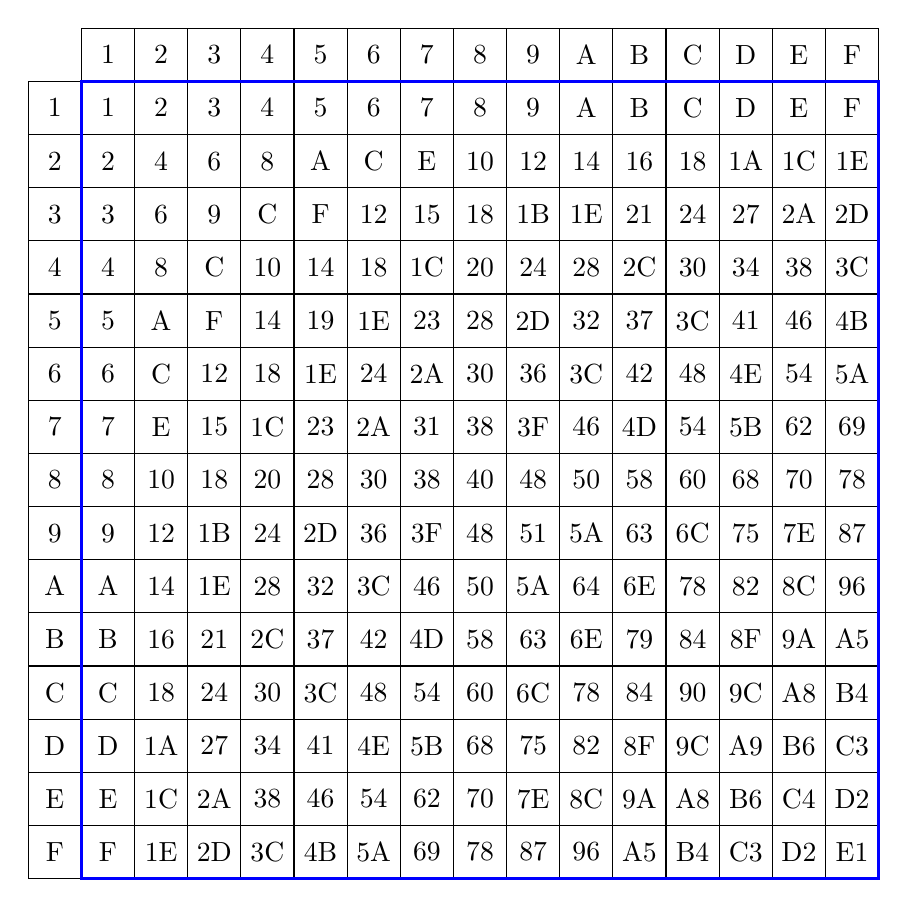
\begin{tikzpicture}[scale=0.675]
		% grid definition
		\draw (-1,0) grid (15,15);
		\draw (0,10) grid (15,16);
		\draw[line width=1pt, color=blue] (0,0) rectangle (15,15);
		
		% fill numbers
		\foreach \x in {1,2,3,...,15}
		\foreach \y in {1,2,3,...,15}
		\draw[shift={(-.5,-.5)}] (\x ,\y) node {\pgfmathHex{\number\numexpr\x*(16-\y)}\pgfmathresult\relax};
		
		% fill first row
		\foreach \x in {1,2,3,...,15}
		\draw[shift={(-.5,-.5)}] (\x , 16) node {\pgfmathHex{\x}\pgfmathresult};
		
		% fill first column
		\foreach \y in {1,2,3,...,15}
		\draw[shift={(-.5,-.5)}] (0, 16-\y) node {\pgfmathHex{\y}\pgfmathresult};
	\end{tikzpicture}
	\caption{Tavola Prodotti esadecimale}
	\label{tab:TavolaPitagoricaesadecimale}
\end{table}
\begin{table}[H]
	\centering
	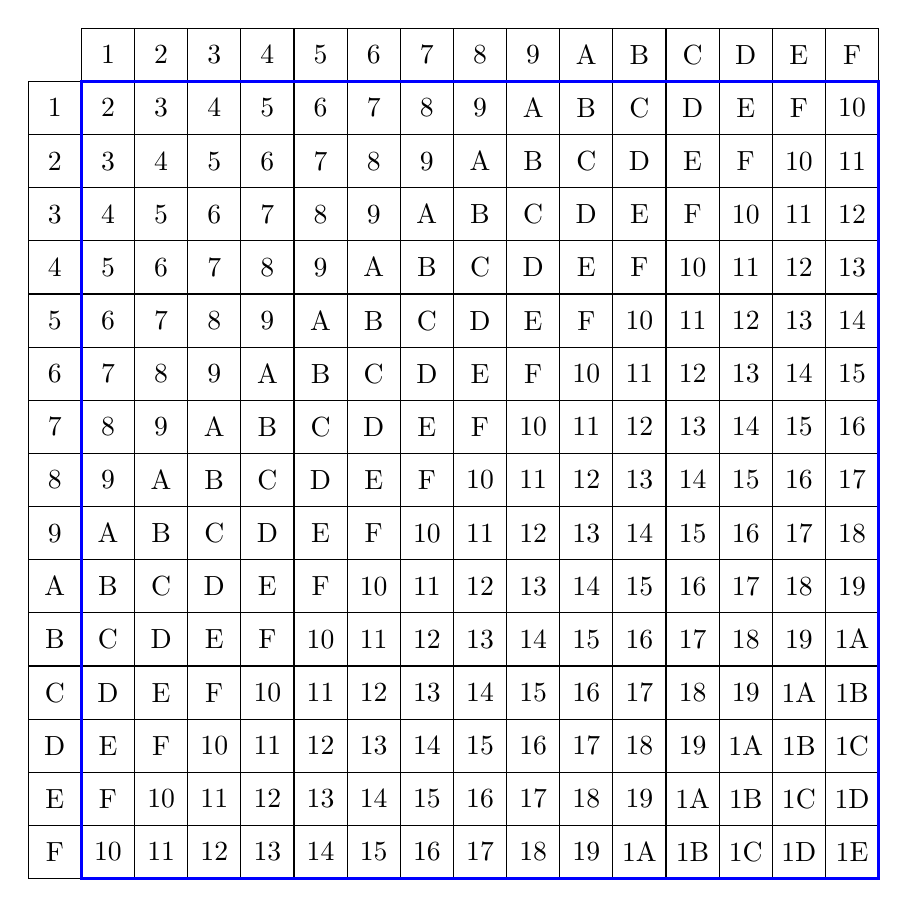
\begin{tikzpicture}[scale=0.675]
		% grid definition
		\draw (-1,0) grid (15,15);
		\draw (0,10) grid (15,16);
		\draw[line width=1pt, color=blue] (0,0) rectangle (15,15);
		
		% fill numbers
		\foreach \x in {1,2,3,...,15}
		\foreach \y in {1,2,3,...,15}
		\draw[shift={(-.5,-.5)}] (\x ,\y) node {\pgfmathHex{\number\numexpr\x+(16-\y)}\pgfmathresult\relax};
		
		% fill first row
		\foreach \x in {1,2,3,...,15}
		\draw[shift={(-.5,-.5)}] (\x , 16) node {\pgfmathHex{\x}\pgfmathresult};
		
		% fill first column
		\foreach \y in {1,2,3,...,15}
		\draw[shift={(-.5,-.5)}] (0, 16-\y) node {\pgfmathHex{\y}\pgfmathresult};
	\end{tikzpicture}
	\caption{Tavola somma esadecimale}
	\label{tab:Tavolaaddizioniesadecimale}
\end{table}
\subsection{Base otto}
\subsubsection{Conversioni}



\begin{table}[H]
	\centering
	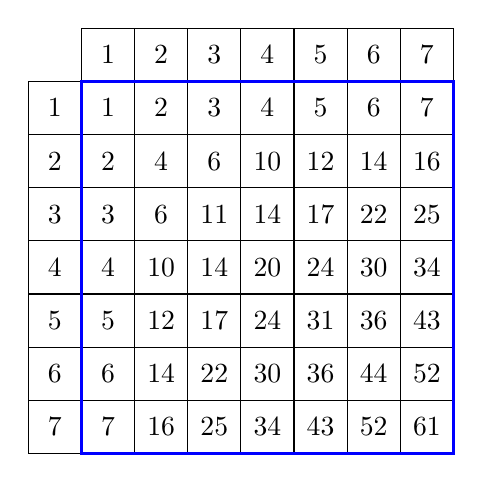
\begin{tikzpicture}[scale=0.675]
		% grid definition
		\draw (-1,0) grid (7,7);
		\draw (0,7) grid (7,8);
		\draw[line width=1pt, color=blue] (0,0) rectangle (7,7);
		
		% fill numbers
		\foreach \x in {1,2,3,...,7}
		\foreach \y in {1,2,3,...,7}
		\draw[shift={(-.5,-.5)}] (\x ,\y) node { \pgfmathoct{\number\numexpr\x*(8-\y)}\pgfmathresult\relax};
		
		% fill first row
		\foreach \x in {1,2,3,...,7}
		\draw[shift={(-.5,-.5)}] (\x , 8) node {\pgfmathoct{\x}\pgfmathresult};
		
		% fill first column
		\foreach \y in {1,2,3,...,7}
		\draw[shift={(-.5,-.5)}] (0, 8-\y) node {\pgfmathoct{\y}\pgfmathresult};
	\end{tikzpicture}
	\caption{Tavola Pitagorica ottale}
	\label{tab:TavolaPitagoricaottale}
\end{table}
\begin{table}[H]
	\centering
	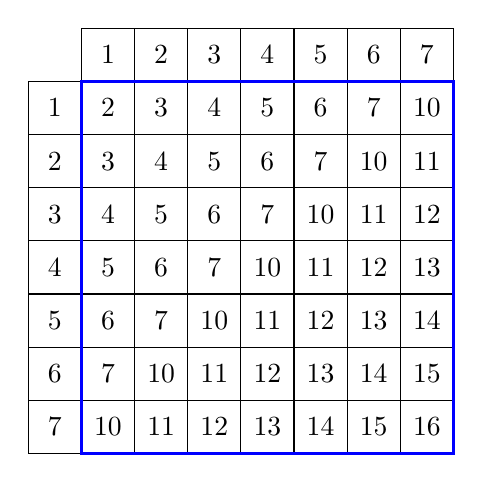
\begin{tikzpicture}[scale=0.675]
		% grid definition
		\draw (-1,0) grid (7,7);
		\draw (0,7) grid (7,8);
		\draw[line width=1pt, color=blue] (0,0) rectangle (7,7);
		
		% fill numbers
		\foreach \x in {1,2,3,...,7}
		\foreach \y in {1,2,3,...,7}
		\draw[shift={(-.5,-.5)}] (\x ,\y) node { \pgfmathoct{\number\numexpr\x+(8-\y)}\pgfmathresult\relax};
		
		% fill first row
		\foreach \x in {1,2,3,...,7}
		\draw[shift={(-.5,-.5)}] (\x , 8) node {\pgfmathoct{\x}\pgfmathresult};
		
		% fill first column
		\foreach \y in {1,2,3,...,7}
		\draw[shift={(-.5,-.5)}] (0, 8-\y) node {\pgfmathoct{\y}\pgfmathresult};
	\end{tikzpicture}
	\caption{Tavola Somma ottale}
	\label{tab:Tavolasommaottale}
\end{table}

	\chapter{Codifica Braille}
\label{Cha:CodificaBraille}
\begin{table}[H]
\begin{tabular}{cccc}
				\mytable{
					\braille{a} & a 1 \\
					\braille{b} & b 2 \\
					\braille{c} & c 3 \\
					\braille{d} & d 4 \\
					\braille{e} & e 5 \\
					\braille{f} & f 6 \\
					\braille{g} & g 7 \\
					\braille{h} & h 8 \\
					\braille{i} & i 9 \\
					\braille{j} & j 0 \\
					\braille{k} & k \\
					\braille{l} & l \\
					\braille{m} & m \\
					\braille{n} & n \\
					\braille{o} & o \\
				}&
				\mytable{
					\braille{p} & p \\
					\braille{q} & q \\
					\braille{r} & r \\
					\braille{s} & s \\
					\braille{t} & t \\
					\braille{u} & u \\
					\braille{v} & v \\
					\braille{w} & w \\
					\braille{x} & x \\
					\braille{y} & y \\
					\braille{z} & z \\
				}  &
				\mytable{
					\braille{{Capital}} & \{Maiuscolo\}\\
					\braille{{Upper}} & \{In alto\} \\
					%\braille{{Italic}} & \{Italic\} \\
				}
				&
				\mytable{
					\braille{{Number}} & \{Numero\} \\	
					\braille{{Letter}} & \{Lettera\} \\
				}   \\ 
				

			\end{tabular}
\caption[Codifica Braille]{ Codifica Braille (\copyright 1998-2010 William Park Licenza LPPL)}\label{tsd:}
\label{tab:CodificaBraille}
\end{table}
					
					
Ciao Mondo
					\braille{Ciao Mondo}
					
					1980
					\braille{{Number}1980}
	\chapter{Codifica ASCII}
\label{Cha:CodificaASCII}
	\settowidth{\gnat}{NUL}
	\settowidth{\gnam}{b1}
\begin{table}[H]

%	\begin{tabular}{r@{\hspace{0mm}}l}
%		& 
%		
%		\begin{tabular}{|N{\gnam}|*8{N{\gnat}}|}
%			\hline
%			$b_7$	& 0 & 0 & 0 & 0 & 1 & 1 & 1 & 1 \tabularnewline
%			
%			$b_6$	& 0 & 0 & 1 & 1 & 0 & 0 & 1 & 1 \tabularnewline
%			$b_5$	& 0 & 1 & 0 & 1 & 0 & 1 & 0 & 1 \tabularnewline
%			\hline
%		\end{tabular} 
%		\tabularnewline	
%		\begin{tabular}{|N{\gnam}|*4{N{\gnam}}}
%			\hline
%			$h_0$& $b_3$ &  $b_2$& $b_1$ & $b_0$ \tabularnewline 
%			\hline
%			0	& 0 & 0 & 0 & 0 \tabularnewline
%			1	& 0 & 0 & 0 & 1 \tabularnewline
%			2	& 0 & 0 & 1 & 0 \tabularnewline
%			3	& 0 & 0 & 1 & 1 \tabularnewline
%			4	& 0 & 1 & 0 & 0 \tabularnewline
%			5	& 0 & 1 & 0 & 1 \tabularnewline
%			6	& 0 & 1 & 1 & 0 \tabularnewline
%			7	& 0 & 1 & 1 & 1 \tabularnewline
%			8	& 1 & 0 & 0 & 0 \tabularnewline
%			9	& 1 & 0 & 0 & 1 \tabularnewline
%			A	& 1 & 0 & 1 & 0 \tabularnewline
%			B	& 1 & 0 & 1 & 1 \tabularnewline
%			C	& 1 & 1 & 0 & 0 \tabularnewline
%			D	& 1 & 1 & 0 & 1 \tabularnewline
%			E	& 1 & 1 & 1 & 0 \tabularnewline
%			F	& 1 & 1 & 1 & 1 \tabularnewline
%			\hline
%		\end{tabular} 
%		&
%		\begin{tabular}{|N{\gnam}|*8{N{\gnat}}|}
%			& 0 & 1 & 2 &  3& 4 & 5 & 6 & 7 \tabularnewline
%			\hline
%			0	& NUL & DLE & SP & 0 & @ & P & ` & p \tabularnewline
%			1	& SOH & DC1 & !  & 1 & A & Q & a & q \tabularnewline
%			2	& STX & DC2 & "  & 2 & B & R & b & r \tabularnewline
%			3	& ETX & DC3 & \# & 3 & C & S & c & s \tabularnewline
%			4	& EOT & DC4 & \$ & 4 & D & T & d & t \tabularnewline
%			5	& ENO & NAK & \% & 5 & E & U & e & u \tabularnewline
%			6	& ACK & SYN & \& & 6 & F & V & f & v \tabularnewline
%			7	& BEL & ETB & '  & 7 & G & W & g & w \tabularnewline
%			8	& BS  & CAN &  ( & 8 & H & X & h & x \tabularnewline
%			9	& HT  & EM  &  ) & 9 & I & Y & i & y \tabularnewline
%			10	& LF  & SUB & *  & : & J & Z & j & z \tabularnewline
%			11	& VT  & ESC & +  & ; & K & [  & k & \{ \tabularnewline
%			12	& FF  & FS  & ,  & < & L & \textbackslash & l & | \tabularnewline
%			13	& CR  & GS  & -  & = & M & ] & m & \} \tabularnewline
%			14	& SO  & RS  & .  & > & N & \^{}& n & \~{} \tabularnewline
%			15	& SI  & US  &  / & ? & O & \_ & o & DEL \tabularnewline
%			\hline
%		\end{tabular} 
%		\tabularnewline
%	\end{tabular}
\begin{tabular}{|M{\gnam}|*4{M{\gnam}}|M{\gnam}|*8{M{\gnat}}|}
	\cline{6-14}
	\multicolumn5{c|}{\pilH}	&$b_7$	& 0 & 0 & 0 & 0 & 1 & 1 & 1 & 1 \tabularnewline
	\multicolumn5{c|}{}		&$b_6$	& 0 & 0 & 1 & 1 & 0 & 0 & 1 & 1 \tabularnewline
	\multicolumn5{c|}{\pilD}	&$b_5$	& 0 & 1 & 0 & 1 & 0 & 1 & 0 & 1 \tabularnewline
	\hline
	$h_0$& $b_3$ &  $b_2$& $b_1$ & $b_0$ && 0 & 1 & 2 &  3& 4 & 5 & 6 & 7\pilH\pilD\tabularnewline
	\hline
	0	& 0 & 0 & 0 & 0 & 0	& NUL & DLE & SP & 0 & @ & P & ` & p\pilH\tabularnewline
	1	& 0 & 0 & 0 & 1 & 1	& SOH & DC1 & !  & 1 & A & Q & a & q \tabularnewline
	2	& 0 & 0 & 1 & 0 & 2	& STX & DC2 & \string"  & 2 & B & R & b & r \tabularnewline
	3	& 0 & 0 & 1 & 1 & 3	& ETX & DC3 & \# & 3 & C & S & c & s \tabularnewline
	4	& 0 & 1 & 0 & 0 & 4	& EOT & DC4 & \$ & 4 & D & T & d & t \tabularnewline
	5	& 0 & 1 & 0 & 1 & 5	& ENO & NAK & \% & 5 & E & U & e & u \tabularnewline
	6	& 0 & 1 & 1 & 0 & 6	& ACK & SYN & \& & 6 & F & V & f & v \tabularnewline
	7	& 0 & 1 & 1 & 1 & 7	& BEL & ETB & '  & 7 & G & W & g & w \tabularnewline
	8	& 1 & 0 & 0 & 0 & 8	& BS  & CAN &  ( & 8 & H & X & h & x \tabularnewline
	9	& 1 & 0 & 0 & 1 & 9	& HT  & EM  &  ) & 9 & I & Y & i & y \tabularnewline
	A	& 1 & 0 & 1 & 0 & 10& LF  & SUB & *  & : & J & Z & j & z \tabularnewline
	B	& 1 & 0 & 1 & 1 & 11& VT  & ESC & +  & ; & K & [  & k & \{ \tabularnewline
	C	& 1 & 1 & 0 & 0 & 12& FF  & FS  & ,  & < & L & \textbackslash & l & | \tabularnewline
	D	& 1 & 1 & 0 & 1 & 13& CR  & GS  & -  & = & M & ] & m & \} \tabularnewline
	E	& 1 & 1 & 1 & 0 & 14& SO  & RS  & .  & > & N & \textasciicircum& n & \textasciitilde \tabularnewline
	F	& 1 & 1 & 1 & 1 & 15& SI  & US  &  / & ? & O & \_ & o & DEL\rule[-1.5ex]{0pt}{0pt}\tabularnewline
	\hline
\end{tabular}
	\caption{Codifica ASCII}
\end{table}
	\chapter{Algebra di Boole}
\label{cha:AlgebradiBoole}
%\FloatBarrier
\section{Variabili e funzioni booleane}
\label{sec:VariabiliBooleane}
Una variabile booleana\index{Variabile!booleana} è una variabile che può assumere solo due valori, che possono essere indicati o  con\nobs$0$\nobs e\nobs$1$ o con $basso$\nobs e\nobs$alto$, con $vero$\nobs o \nobs$falso$. Nella realtà, a questi valori sono  associati valori arbitrari es: $+5\si{\volt}$ $-5\si{\volt}$, $+12\si{\volt}$ $-12\si{\volt}$. 

 Un sistema si trova in un determinato stato a seconda del valore che assumono le variabili booleane associate.   Vi sono due variabili  particolari la variabile\nobs$0$ che assume solo il valore\nobs$0$ e la variabile \nobs$1$ che assume solo il valore\nobs$1$. 

Una funzione (operazione) booleana\index{Funzione!booleana} è una relazione  che ha in ingresso delle variabili indipendenti e in uscita una variabile dipendente.

A ogni sistema è associata una tabella detta tavola di verità\index{Tavola di verità}. Una tavola di verità rappresenta in forma tabellare, in base agli stati del sistema in entrata, lo stato del sistema in uscita. Si può facilmente provare %, utilizzando la tavola~\vref{tab:statisistema},  
che la tabella\vref{tab:totfunzzionilogiche} rappresenta tutte le funzioni logiche con due valori in entrata.

Due funzioni logiche sono equivalenti\index{Funzione!booleana!equivalente} se hanno la stessa tavola di verità. Esempio di questo sono la tabella\nobs\vref{tab:tabVeritaEOR} e la tabella\nobs\vref{tab:tabVeritaEOR2} che sono fra di loro equivalenti. 

Un metodo grafico per rappresentare una funzione logica  è il circuito che si ottiene combinando i simboli  elencati nella tabella\nobs\vref{tab:Portelogichetavver}. Un esempio di ciò sono  i due circuiti\nobs\vref{Tab:circuito2e3} che rappresentano entrambi la funzione $XOR$\index{Funzione!booleana!XOR}  ottenuta come combinazione di $AND$\index{Funzione!booleana!AND} e $OR$\index{Funzione!booleana!OR}

Principio di dualità: Se una funzione logica è vera, allora è vera la funzione che si ottiene scambiando $AND$ con  $OR$ e  $0$ con $1$ e viceversa.

\begin{table} %[H]
	%\centering
	\begin{tabular}{cccccccccccccccccc}
	\toprule
	A & B & $0$ & NOR & $\overline{A}$ &  &  & $\overline{B}$ & XOR & NAND & AND & XNOR &  & B & A &  & OR & $1$ \\ 
	\midrule
	1 & 1 & 0 & 0 & 0 & 0 & 0 & 0 & 0 & 0 & 1 & 1 & 1 & 1 & 1 & 1 & 1 & 1 \\ 
	1 & 0 & 0 & 0 & 0 & 0 & 1 & 1 & 1 & 1 & 0 & 0 & 0 & 0 & 1 & 1 & 1 & 1 \\ 
	0 & 1 & 0 & 0 & 1 & 1 & 0 & 0 & 1 & 1 & 0 & 0 & 1 & 1 & 0 & 0 & 1 & 1 \\ 
	0 & 0 & 0 & 1 & 1 & 0 & 0 & 1 & 0 & 1 & 0 & 1 & 1 & 0 & 0 & 1 & 0 & 1 \\ 
	\bottomrule
	\end{tabular}
	\caption{Funzioni logiche}
	\label{tab:totfunzzionilogiche}
\end{table}
\subsection{Esempi}
\label{sec:Esempiofunzlog}
Definire, utilizzando le funzioni logiche:

$tavolo=(legno,ferro,3gambe,4gambe,piano)$,

$auto=(3 porte,5 porte,ruote,motore)$, 

$penna=(sfera,stilografica,rossa,nera,verde,cancellabile,indelebile)$

Una cassaforte ha quattro lucchetti, x, y, v, w, che devono essere tutti aperti affinché la
cassaforte si apra.  Tre persone A, B, C,  hanno le  chiavi. A possiede le chiavi v e y; 
B ha le chiavi v e x e C tiene w e y. Le variabili A, B, C sono uguali a uno se la persona corrispondente è presente, altrimenti sono uguali a zero. Costruire la tavola
della verità della funzione $Y=f(A,B,C)$. La funzione  vale uno se e solo se la cassaforte può essere  aperta,
 esprimere f in forma algebrica. Per risolvere almeno la prima parte dell'esercizio costruiamo una tabella  che leghi le chiavi alle tre persone.
\begin{table}
	    \centering
		\begin{tabular}{c|cccc}
			& \textbf{x} & \textbf{y} &\textbf{v}& \textbf{w}\\
			\toprule 
			\textbf{A} &  & \textbullet &\textbullet & \\ 
			\textbf{B} & \textbullet &  & \textbullet& \\ 
			\textbf{C} &  & \textbullet & & \textbullet\\ 
			\bottomrule
		\end{tabular}
	\caption[]{Persone e chiavi}
	\label{tab:personeechiavi}
\end{table} 
Quindi: il sistema (la cassaforte aperta o chiusa), dipende da tre variabili $A$, $B$ e $C$ che assumono solo due valori $1$ se la chiave è presente o $0$ altrimenti. In uscita $Y$ può assumere due valori $1$ se la cassaforte è aperta o $0$ nell'altro caso. 

La tabella~\vref{tab:personeechiavi} permette di costruire la tavola di verità\nobs\vref{tab:tavolaveritacasaforte} della funzione. La tabella, dipendendo da tre variabili in ingresso, ha otto stati. Iniziamo a costruire la tavola di verità del sistema. Nella prima riga abbiamo che $A=0$, $B=0$ e $C=0$, poiché nessuna chiave è presente, la cassaforte rimane chiusa quindi $Y=0$. Nella seconda riga abbiamo che $A=0$, $B=0$ e $C=1$,  due chiavi sono presenti ma \nobs\vref{tab:personeechiavi} ci dice che queste non bastano e la cassaforte è chiusa e quindi $Y=0$. Il discorso è analogo  per le righe rimanenti. Nella riga quattro abbiamo che $A=0$, $B=1$ e $C=1$  sono presenti quattro chiavi e la cassaforte viene aperta per cui $Y=1$.  Stesso discorso la riga otto e anche in questo caso $Y=1$.
\begin{table}
		\centering
\begin{tabular}{c|c|c|c|c}
	& \textbf{A} & \textbf{B} & \textbf{C} & \textbf{Y} \\
	\toprule 
	1& 0 & 0 & 0 & 0 \\ 
	2& 0 & 0 & 1 &  0\\ 
	3& 0 & 1 & 0 &  0\\ 
	4& 0 & 1 & 1 &  1\\ 
	5& 1 & 0 & 0 &  0\\ 
	6& 1 & 0 & 1 &  0\\ 
	7& 1 & 1 & 0 &  0\\ 
	8& 1 & 1 & 1 &  1\\ 
	\bottomrule
\end{tabular} 
	\caption{Tavola di verità}
	\label{tab:tavolaveritacasaforte}
\end{table}
\section{Tavole di verità}
\label{sec:TavoleDiVeritA}
\begin{figure} %[H]
\centering
	\pagestyle{empty}
	% Set the overall layout of the tree
\tikzstyle{level 1}=[level distance=3.5cm, sibling distance=3.5cm]
\tikzstyle{level 2}=[level distance=3.5cm, sibling distance=2cm]
\tikzstyle{level 3}=[level distance=3cm, sibling distance=0.8cm] 
% Define styles for bags and leafs
%\tikzstyle{bag} = [text width=4em, text centered]
\tikzstyle{bag} =[shape=circle,draw,
text centered]
\begin{tikzpicture}[grow=right, sloped]
\matrix [row sep=1em] 
{
	\node[bag] {0}
	child{   
		node[bag] {0}
		child{
			node[bag] {0}
			child{
				node[bag]{0}
			}
			child{
				node[bag]{1}
			}
		}
		child {
			node[bag] {1}
			child{
				node[bag]{0}
			}
			child{
				node[bag]{1}
			}		
		}
	}
	child{
		node[bag]{1}
		child{
			node[bag] {0}
			child{
				node[bag]{0}
			}
			child{
				node[bag]{1}
			}
		}
		child {
			node[bag] {1}
			child{
				node[bag]{0}
			}
			child{
				node[bag]{1}
			}
		}   
	};
	&\\
	\draw (0,0) --  (10.5,0);
	\draw (0.0,1pt) -- (0.0,-3pt)
	node[anchor=north] {1};
	\draw (3.5,1pt) -- (3.5,-3pt)
	node[anchor=north] {2};
	\draw (7,1pt) -- (7,-3pt)
	node[anchor=north] {3};
	\draw (10,1pt) -- (10,-3pt)
	node[anchor=north] {4};\\
	\node[bag] {0}
	child{   
		node[bag] {0}
		child{
			node[bag] {0}
			child{
				node[bag]{0}
			}
			child{
				node[bag]{1}
			}
		}
		child {
			node[bag] {1}
			child{
				node[bag]{0}
			}
			child{
				node[bag]{1}
			}		
		}
	}
	child{
		node[bag]{1}
		child{
			node[bag] {0}
			child{
				node[bag]{0}
			}
			child{
				node[bag]{1}
			}
		}
		child {
			node[bag] {1}
			child{
				node[bag]{0}
			}
			child{
				node[bag]{1}
			}
		}   
	};\\
};
\end{tikzpicture}
	\caption{Stati del sistema}
	\label{tab:statisistema}
\end{figure}

Le funzioni logiche sono divise in gruppi. Il primo è formato dalle funzioni AND\index{Funzione!booleana!AND}, OR\index{Funzione!booleana!OR} e NOT\index{Funzione!booleana!NOT}. Segue il gruppo formato solo da NAND\index{Funzione!booleana!NAND}. Infine quello composto solo  da NOR\index{Funzione!booleana!NOR}. Ogni gruppo è tale perché in grado di generare le rimanenti funzioni. La figura~\vref{tab:Portelogichetavver} riporta le tavole di verità di queste funzioni. 

Combinando fra di loro le funzioni  otteniamo altre funzioni come viene per esempio, nella tabella~\vref{tab:ComposizionePorte}. 

La tabella~\vref{tab:statisistema} da in verticale di quante righe deve avere una tavola di verità.  Con una variabile due righe,  due variabili  otteniamo quattro righe etc. Mentre in orizzontale,in base al numero delle variabili, percorrendo i grafi da sinistra verso destra, avremo tutti i possibili stati di un sistema.
\subsection{Funzione AND}
\label{sub:funzioneAND}
La funzione AND\index{Funzione!booleana!AND} ha due valori in entrata ed  un valore in uscita che è vero solo quando sono veri entrambi i valori in entrata. Il simbolo che la rappresenta l'operazione è il prodotto.

Nella realtà casi in cui si usano funzioni AND sono molteplici. In genere si usa una funzione AND\index{Funzione!booleana!AND} quando  si eseguono due azioni in contemporaneamente come per esempio nel dispositivi di azionamento di una pressa in cui si premono contemporaneamente due pulsanti in modo da impegnare entrambe le mani, evitando così incidenti. 

Un esempio della funzione AND\index{Funzione!booleana!AND} è il seguente circuito\nobs\vref{tab:elettricoAND}. Abbiamo un circuito con due pulsanti in serie.  La lampada si accende solo premendo solo contemporaneamente i due interruttori.
\begin{table}[H]
	\centering
	\begin{circuitikz} \draw
		(0,0)--(0,2)
		(5,0)--(5,2)
		(0,0) to[lamp] (2,0)
		(2,0) to[battery] (5,0)
		(0,2) to[opening switch] (3,2)
		(3,2) to[opening switch] (5,2);
	\end{circuitikz}
	\caption{Circuito AND}
	\label{tab:elettricoAND}
\end{table}
	
La tabella\nobs\ref{tab:Portelogichetavver} mostra la tavola di verità\index{Tavola di verità!AND} della $AND$\index{Funzione!booleana!AND} e il simbolo grafico associato.
\subsection{Funzione OR}
\label{sub:funzioneOR}
La funzione OR\index{Funzione!booleana!OR} ha due valori in entrata e un valore in uscita. Questo valore è vero quando almeno uno dei valori in ingresso è vero. Il simbolo che la rappresenta è la somma. 

Un esempio dell'uso della funzione OR\index{Funzione!booleana!OR} è l'impianto di illuminazione di una stanza in cui due interruttori distinti permettono di accendere una lampadina.

Un circuito in parallelo, come il circuito\nobs\vref{tab:ZunzioneOR}, rappresenta la funzione OR\index{Funzione!booleana!OR}. Per accendere la lampadina basta premere almeno un interruttore.
\begin{table}
	\centering
	\begin{circuitikz} \draw
		(0,0)--(0,2)
		(5,0)--(5,2)
		(0,0) to[lamp] (2,0)
		(2,0) to[battery] (5,0)
		(0,2)--(1,2)
		(1,1)--(1,3)
		(4,1)--(4,3)
		(4,2)--(5,2)
		(1,3) to[opening switch] (4,3)
		(1,1) to[opening switch] (4,1);
	\end{circuitikz}
	\caption{Circuito OR}
	\label{tab:ZunzioneOR}
\end{table}
La tabella\nobs\ref{tab:Portelogichetavver} mostra la tavola di verità\index{Tavola di verità!OR} della OR\index{Funzione!booleana!OR} e il simbolo grafico associato.
\subsection{Funzione NOT}
\label{sub:funzionenot}
La funzione NOT ha un solo valore in entrata e un solo valore in uscita. Il valore in uscita è l'opposto a quello in ingresso. Il simbolo che rappresenta l'operazione è un trattino che si pone sopra la variabile.

Un esempio dell'uso della funzione NOT\index{Funzione!booleana!NOT} è per esempio l'interruttore della luce di cortesia di un'auto che si accende aprendo la portiera.

Un circuito come il circuito\nobs\vref{tab:CircuitoNOT} rappresenta la funzione NOT. La tabella\nobs\ref{tab:Portelogichetavver} mostra la tavola di verità\index{Tavola di verità!NOT} della NOT e il simbolo grafico associato.
\begin{table}
	\centering
	 \begin{circuitikz} \draw
		(0,0)--(0,2)
		(6,0)--(6,2)
		(0,1) to[lamp] (6,1)
		(0,2)--(3,2)
		(3,2) to[battery,v_<=$+-$] (6,2)
		(0,0) to[opening switch] (3,0)
		(3,0) to[battery,v_<=$+-$] (6,0);
	\end{circuitikz}
	\caption{Circuito NOT}
	\label{tab:CircuitoNOT}
\end{table}
	
\subsection{Funzione XOR}
\label{sub:funzioneXOR}
La funzione XOR\index{Funzione!booleana!XOR} ha due valori in entrata ed un valore in uscita che è vero quando solo uno dei valori in ingresso è vero.

Il circuito\nobs\vref{tab:circuitoXOR} rappresenta un OR esclusivo. Sono due gruppi di pulsanti in parallelo messe in serie. La seconda serie di pulsanti sono i negati dei precedenti. Quando vien premuto il primo pulsante $A$ il pulsante $\overline{A}$ del secondo circuito viene aperto e viceversa, analogamente per il pulsante $B$. In questo circuito la corrente passa e  lampadina si accende, solo se è premuto un solo pulsante ma non entrambi.

La tabella\nobs\ref{tab:Portelogichetavver} mostra la tavola di verità della XOR\index{Tavola di verità!XOR} e il simbolo grafico associato.
\begin{table} %[H]
		\centering
		\begin{circuitikz} \draw
			(0,0)--(0,2)
			(7,0)--(7,2)
			(0,0) to[lamp] (3,0)
			(3,0) to[battery] (7,0)
			(0,2)--(1,2)
			(1,1)--(1,3)
			(3,1)--(3,3)
			(3,2)--(4,2)
			(4,1)--(4,3)
			(6,1)--(6,3)
			(6,2)--(7,2)
			(1,3) to[opening switch=$A$] (3,3)
			(1,1) to[opening switch=$B$] (3,1)
			(4,1) to[closing switch=$\overline{B}$] (6,1)
			(4,3) to[closing switch=$\overline{A}$] (6,3);
		\end{circuitikz}
	\caption{Circuito XOR}
	\label{tab:circuitoXOR}
	\end{table}
\subsection{Funzione NAND}
\label{sub:funzioneNAND}
La funzione NAND\index{Funzione!booleana!NAND} ha due valori in entrata ed ha un valore in uscita che è falso solo quando sono veri entrambi i valori in entrata.

La tabella\nobs\ref{tab:Portelogichetavver} mostra la tavola di verità\index{Tavola di verità!NAND} della $NAND$\index{Funzione!booleana!NAND} e il simbolo grafico associato. La $NAND$ è la negazione di $AND$\index{Funzione!booleana!AND}.

\subsection{Funzione NOR}
\label{sub:funzioneNOR}
La funzione NOR\index{Funzione!booleana!NOR} ha due valori in entrata ed ha un valore in uscita che è vero solo quando sono falsi entrambi i valori in entrata.

La tabella\nobs\ref{tab:Portelogichetavver} mostra la tavola di verità\index{Tavola di verità!NOR} della NOR\index{Funzione!booleana!NOR} e il simbolo grafico associato. La NOR è la negazione di OR 
\subsection{Funzione XNOR}
\label{sub:funzioneXNOR}
La funzione XNOR\index{Funzione!booleana!XNOR} ha due valori in entrata ed ha un valore in uscita che è vero solo quando sono falsi entrambi i valori in entrata o quando sono entrambi veri. 

La tabella\nobs\ref{tab:Portelogichetavver} mostra la tavola di verità\index{Tavola di verità!XNOR} della XNOR e il simbolo grafico associato. La XNOR è la negazione di XOR 

Il circuito\nobs\vref{tab:circuitoXNOR} è formato da due blocchi di pulsanti in serie messi in parallelo. Quando vien premuto il primo pulsante $A$ il pulsante $\overline{A}$ del secondo circuito viene aperto e viceversa, analogamente per il pulsante $B$. La lampadina si accende o quando entrambi i pulsanti $A$ e $B$ sono premuti o entrambi i  pulsanti $A$ e $B$ sono tenuti alzati.
\begin{table}[H]
	\centering
	\begin{circuitikz} \draw
		(0,0)--(0,2)
		(7,0)--(7,2)
		(0,0) to[lamp] (3,0)
		(3,0) to[battery] (7,0)
		(0,2)--(1,2)
		(1,1)--(1,3)
		(6,1)--(6,3)
		(6,2)--(7,2)
		(1,3) to[opening switch=$A$] (4,3)
		(4,3) to[opening switch=$B$] (6,3)
		(1,1) to[closing switch=$\overline{A}$] (4,1)
		(4,1) to[closing switch=$\overline{B}$] (6,1);
	\end{circuitikz}
	\caption{Circuito XNOR}
	\label{tab:circuitoXNOR}
\end{table}
Come si è detto a una funzione logica è possibile associare una tavola di verità\index{Tavola di verità!Costruire}. Un esempio di costruzione  è la tabella~\vref{tab:tabVeritaEOR}. Il metodo usato è molto semplice,  prevede di suddividere la funzione nelle sue componenti e risolverle partendo da sinistra verso destra. Questo deve essere fatto rispettando le convenzioni di precedenza, cioè le negazioni (funzione NOT), poi i prodotti (Funzione AND\index{Funzione!booleana!AND}), e infine le somme (Funzione OR\index{Funzione!booleana!OR}).Possiamo cambiare le  precedenze mettendo fra  delle parentesi le operazioni che devono essere eseguite prima.
In conclusione, abbiamo parlato di tavola di verità\index{Tavola di verità}, circuito, funzione logica, che sono concetti fra loro equivalenti\vref{tab:FunzioneTavolaCircuito} e fra loro connessi.
\begin{table} 
	\centering
	\begin{tikzpicture}[very thick,node distance=5cm,text centered,minimum size=3cm]
		\node [circle, draw] (a) {Funzione logica};
		\node [circle, draw] (b) [above right=of a] {Tavola di verità};
		\node [circle, draw] (c) [above left=of a]{Circuito};
		\draw [<->] (a) to (b);
		\draw [<->] (b) to (c);
		\draw [<->] (c) to (a);
	\end{tikzpicture}
	\caption{Funzione, Tavola e Circuito}
	\label{tab:FunzioneTavolaCircuito}
\end{table}
\begin{table}
	\centering
	\begin{tabular}{@{}cc@{\hspace{2cm}}cc@{}}
	\begin{truthtable}{AND}
	\toprule
	$A$&$B$&$AB$\\
	\midrule           
	0&0&0\\
	1&0&0\\
	0&1&0\\
	1&1&1\\
	\bottomrule
	\end{truthtable}
	& \cport{and} &
	\begin{truthtable}{NAND}
	\toprule
	$A$&$B$&$A\mathbin{\overline{\wedge}}B$\\
	\midrule
	0&0&1\\
	1&0&1\\
	0&1&1\\
	1&1&0\\
	\bottomrule
	\end{truthtable}
	& \cport{nand} \\
	\addlinespace[3ex]
	\begin{truthtable}{OR}
	\toprule
	$A$&$B$&$A+B$\\
	\midrule         
	0&0&0\\
	1&0&1\\
	0&1&1\\
	1&1&1\\
	\bottomrule
	\end{truthtable}
	& \cport{or} &
	\begin{truthtable}{NOR}
	\toprule
	$A$&$B$&$A\mathbin{\overline{\vee}}B$\\
	\midrule
	0&0&1\\
	1&0&0\\
	0&1&0\\
	1&1&0\\
	\bottomrule
	\end{truthtable}
	& \cport{nor} \\
	\addlinespace[3ex]
	\begin{truthtable}{XOR}
	\toprule
	$A$&$B$&$A\XOR B$\\
	\midrule         
	0&0&0\\
	1&0&1\\
	0&1&1\\
	1&1&0\\
	\bottomrule
	\end{truthtable}
	& \cport{xor} &
	\begin{truthtable}{XNOR}
	\toprule
	$A$&$B$&$A\mathbin{\overline{\XOR}}B$\\
	\midrule
	0&0&1\\
	1&0&0\\
	0&1&0\\
	1&1&1\\
	\bottomrule
	\end{truthtable}
	& \cport{xnor} \\
	\addlinespace[3ex]
	\multicolumn{4}{c}{%
		\begin{tabular}{@{}cc@{}}
		\begin{truthtable}[2]{NOT}
		\toprule
		$A$&$\overline{A}$\\
		\midrule         
		0&1\\
		1&0\\
		\bottomrule
		\end{truthtable}
		& \cport{not}
		\end{tabular}}
	\end{tabular}
	\caption{Porte logiche}
	\label{tab:Portelogichetavver}
\end{table} 
\begin{table} %[H]
	\centering
	\begin{tabular}{ccc}
	\toprule
	\begin{circuitikz} \draw
	(0,0) node[and port] (myand) {}
	(1,0) node[not port] (mynot) {}
	(myand.out) -- (mynot.in)
	;\end{circuitikz}&&\begin{circuitikz} \draw
	(0,0) node[nor port]  {}
	;\end{circuitikz} \\
	AND +  NOT &=&NAND \\
	\midrule
	\begin{circuitikz} \draw
	(0,0) node[or port] (myor) {}
	(1,0) node[not port] (mynot) {}
	(myor.out) -- (mynot.in)
	;\end{circuitikz}&& \begin{circuitikz} \draw
	(0,0) node[nor port]  {}
	;\end{circuitikz} \\
	OR +  NOT &=&NOR  \\ 
	\midrule
	\begin{circuitikz} \draw
	(0,0) node[xor port] (myxor) {}
	(1,0) node[not port] (mynot) {}
	(myxor.out) -- (mynot.in)
	;\end{circuitikz}&& \begin{circuitikz} \draw
	(0,0) node[xnor port]  {}
	;\end{circuitikz} \\
	XOR +  NOT &=&XNOR  \\ 
	\bottomrule
	\end{tabular} 
	\caption{Composizione porte}%
	\label{tab:ComposizionePorte}%
\end{table}
\section{Proprietà dell'algebra algebra booleana}
\label{sec:Algebrabooleana}
La tabella\nobs\vref{Tab:AlgebrAbOOLEAN} elenca le principali proprietà delle funzioni AND\index{Funzione!booleana!AND} e OR\index{Funzione!booleana!OR} e mostra come le proprietà delle funzioni siano legate tramite il principio di dualità. Infatti, osservando la tabella si vede come le proprietà elencate a sinistra trovino il loro corrispondente duale a destra e viceversa. La tabella\nobs\vref{Tab:funzlogSemp} mostra come ottenere i risultati. Non vengono dimostrate tutte le relazioni inquarto le altre si ottengono per dualità.

%\altapriorita{Specificare meglio}
Una funzione logica non è unica ma può essere scritta in modi fra di loro equivalenti. La tabella\nobs\vref{Tab:funzlogSemp} mostra come con pochi passaggi si può passare da una funzione logica a una equivalente.
\begin{table}%[H]
\centering
\begin{tabular}{lcl}
\toprule
&PROPRIET\'A&\\
&$\overline{\overline{A}}=A$&\\
$A+0=A$&Elemento neutro&$A\cdot1=A$\\
$A+1=1$&Assorbimento&$A\cdot0=0$\\
$A+A=A$&Idempotenza&$A\cdot A=A$\\
$A+\overline{A}=1$&&$A\cdot\overline{A}=0$\\
$A+B=B+A$&Commutativa&$A\cdot B=B\cdot A$\\
$(A\cdot B)\cdot C=A\cdot(B\cdot C)=A\cdot B\cdot C$&Associativa&$(A+B)+C=A+(B+C)=A+B+C$\\
\midrule
&TEOREMI&\\
\midrule
$A+A\cdot B=A$&&$A\cdot(A+B)=A$\\
$A+\overline{A}\cdot B=A+B$&&$A\cdot (\overline{A}+B)=AB$\\
$(A+B)\cdot(A+C)=A+B\cdot C$&&$A\cdot B+A\cdot C=A\cdot(B+C)$\\
$(A+B)\cdot(\overline{A}+C)=\overline{A}\cdot B+A\cdot C$&&$A\cdot B+\overline{A}\cdot C=(\overline{A}+B)\cdot(A+B)$\\
\midrule
&TEOREMI DI DE MORGAN&\\
\midrule
$\overline{A+B}=\overline{A}\cdot\overline{B}$&&$\overline{A\cdot B}=\overline{A}+\overline{B}$\\
\bottomrule
\end{tabular}
\caption{Teoremi e proprietà algebra di Boole}%
\label{Tab:AlgebrAbOOLEAN}%
\end{table}
\begin{table}
\centering
\begin{tabular}{lcl}
\toprule
%\midrule
PROPRIET\'A&&DIMOSTRAZIONE\\
\midrule
$A+A\cdot B=A$&&$A+A\cdot B=$\\
&&$=A\cdot(1+B)=$\\
&&$=A\cdot1=A$\\ 
\midrule
$A+\overline{A}\cdot B=A+B$&&$A+A\cdot B+\overline{A}\cdot B=$\\
&&$=A+(A+\overline{A})\cdot B=$\\
&&$=A+1\cdot B=$\\
&&$=A+B$\\
\midrule
$(A+B)\cdot(A+C)=A+B\cdot C$&&$(A+B)\cdot(A+C)=$\\
&&$A\cdot A+A\cdot C+A\cdot B+B\cdot C=$\\
&&$=A+A\cdot C+A\cdot B+B\cdot C=$\\
&&$=A\cdot(1+C) +A\cdot B+B\cdot C=$\\
&&$=A\cdot 1 +A\cdot B+B\cdot C=$\\
&&$=A\cdot(1+B)+B\cdot C=$\\
&&$A+B\cdot C$\\
\midrule
$(A+B)\cdot(\overline{A}+C)=\overline{A}\cdot B+A\cdot C$&&$(A+B)\cdot(\overline{A}+C)$\\
&&$\overline{A}\cdot A+ A\cdot C +\overline{A}\cdot B+B\cdot A\cdot C$\\
&&$A\cdot B+\overline{A}\cdot B+B\cdot C$\\
&&$(A+B)\cdot C+\overline{A}\cdot B$\\
&&$(A+\overline{A}\cdot B)\cdot C+\overline{A}\cdot B$\\
&&$A\cdot C+\overline{A}\cdot B\cdot C+\overline{A}\cdot B$\\
&&$A\cdot C+\overline{A}\cdot B(C+1)$\\
&&$A\cdot C+\overline{A}\cdot B$\\
\bottomrule
\end{tabular}
\caption{Semplificazioni}
\label{Tab:funzlogSemp}
\end{table}
\section{Trovare la tavola di verità di una funzione}
\label{sec:Trovaretavolaveritàfunzione}
Per trovare data una funzione, la tavola di verità\index{Tavola di verità}, basta sostituire alle variabili booleane  i valori in ingresso e vedere cosa ha la funzione in uscita. 

Consideriamo la funzione $Y=A\cdot\overline{B}+\overline{A}\cdot B$  possiamo costruire la tabella\nobs\vref{tab:tabVeritaEOR} che fornisce tutti i calcoli necessari. Si procede sostituendo alle variabili tutti i valori possibili e ottenendo dopo i calcoli i risultati della colonna sette 

Analogo ragionamento è per $Y=(A+B)\cdot(\overline{A}+\overline{B})$ e ottenere la tabella\nobs\vref{tab:tabVeritaEOR2}.

Per $Y=\overline{A}\cdot\overline{B}\cdot C+\overline{A}\cdot B\cdot\overline{C}+\overline{A}\cdot B\cdot C+A\cdot B\cdot C$ otteniamo la tavola di verità\nobs\vref{Tab:esempio2bool}\index{Tavola di verità}

La tavola di verità per $Y=\overline{A}\cdot (A+B)+\overline{C}+B\cdot C$ e per $Y=B+\overline{C}$ è\nobs\vref{Tab:Tabveres1}
\begin{table}
	\centering
	\begin{tabular}{ccccccccccc}
		\toprule
		\multicolumn{10}{c}{$A\cdot\overline{B}+\overline{A}\cdot B$} \\ 
		&  &  & 1 & 3 & 2 & 7 & 4 & 6 & 5 \\ 
		A & B &  & $A$&$\cdot$  &$\overline{B}$&$+$& $\overline{A}$ &$\cdot$ &$B$  \\ 
		\cmidrule{1-2}\cmidrule{4-10}
		1 & 1 &  & 1 & 0 & 0 & 0 & 0 & 0 & 1 \\ 
		1 & 0 &  & 1 & 1 & 1 & 1 & 0 & 0 & 0 \\ 
		0 & 1 &  & 0 & 0 & 0 & 1 & 1 & 1 & 1 \\ 
		0 & 0 &  & 0 & 0 & 1 & 0 & 1 & 0 & 0 \\ 
		\bottomrule
	\end{tabular}
	\caption[]{Tavola di verità di $A\cdot\overline{B}+\overline{A}\cdot B$}
	\label{tab:tabVeritaEOR}
\end{table}
\begin{table}
	\centering
	\begin{tabular}{ccccccccccc}
		\toprule
		\multicolumn{10}{c}{$(A+B)\cdot(\overline{A}+\overline{B})$} \\ 
		&  &  & 1 & 3 & 2 & 7 & 4 & 6 & 5 \\ 
		A & B &  & $(A$&$+$  &$B)$ &$\cdot$ &$(\overline{A}$&$+$&$\overline{B})$  \\ 
		\cmidrule{1-2}\cmidrule{4-10}
		1 & 1 &  & 1 & 1 & 1 & 0 & 0 & 0 & 0 \\ 
		1 & 0 &  & 1 & 1 & 0 & 1 & 0 & 1 & 1 \\ 
		0 & 1 &  & 0 & 1 & 1 & 1 & 1 & 1 & 0 \\ 
		0 & 0 &  & 0 & 0 & 0 & 0 & 1 & 1 & 1 \\ 
		\bottomrule
	\end{tabular}
	\caption[]{Tavola di verità di $(A+B)\cdot(\overline{A}+\overline{B})$}
	\label{tab:tabVeritaEOR2}
\end{table}
\section{Trovare la funzione data la tavola di verità}
\label{sec:Trovarefunzionedatatavolaverità}
Per trovare la funzione, nota la tavola di verità\index{Tavola di verità!trovare!funzione}, possiamo utilizzare due metodi\footnote{I due metodi sono duali come si nota leggendo di seguito} 
\subsection{Somma di prodotti canonici} 
Per trovare data la tavola di verità la funzione si usa il metodo della somma di prodotti canonici\index{Somma prodotti canonici!\see{Mintermini}}. Ogni funzione logica si può scrivere come somma di prodotti detti mintermini\index{Mintermini}. Questi prodotti sono costituiti da prodotti di tutte le variabili in forma diretta o negata. Ogni mintermine assume il valore logico 1.

Nell'esempio uno si inizia dalla tavola\nobs\vref{Tab:esempio2bool},  si individuano le righe che hanno come risultato uno e si costruisce la somma dei mintermini. Nella riga due della tavola di verità si ha come risultato uno. Dato che le variabili $A$ $B$ assumono valore zero nel prodotto si inserisce il loro complemento e otteniamo $\overline{A}\cdot \overline{B}\cdot C$.

Si continua con lo stesso criterio ed otteniamo\[Y=2+3+4+8=\overline{A}\cdot\overline{B}\cdot C+\overline{A}\cdot B\cdot\overline{C}+\overline{A}\cdot B\cdot C+A\cdot B\cdot C\] cioè la funzione associata.
\begin{table}
	\centering
	\begin{tabular}{lccc|c}
		&A&B&C&Y\\
		\toprule
		1&0&0&0&0\\
		2&0&0&1&\textbf{1}\\
		3&0&1&0&\textbf{1}\\
		4&0&1&1&\textbf{1}\\
		5&1&0&0&0\\
		6&1&0&1&0\\
		7&1&1&0&0\\
		8&1&1&1&\textbf{1}\\
	\end{tabular}
	\caption[]{Tabella verità di $Y=\overline{A}\cdot\overline{B}\cdot C+\overline{A}\cdot B\cdot\overline{C}+\overline{A}\cdot B\cdot C+A\cdot B\cdot C$}
	\label{Tab:esempio2bool}
\end{table}
%\begin{table}
%	\begin{equation}
%	Y=2+3+4+8=\overline{A}\overline{B}C+\overline{A}B\overline{C}+\overline{A}BC+ABC
%	\end{equation}
%	\caption[]{Funzione booleana esempio 1}
%	\label{tab:esempio2funbool}
%\end{table}
\subsection{Prodotto di somme canoniche}
Per trovare, data la tavola di verità\index{Tavola di verità!trovare!funzione}, la funzione si usa il metodo della prodotti di somme  canoniche\index{Prodotti somme canoniche|see{Maxtermini} }. Ogni funzione logica si può scrivere come prodotto di somme detti maxtermini\index{Maxtermini}. Questi prodotti sono costituiti da somme di tutte le variabili in forma diretta o negata. Ogni maxtermine assume il valore logico 0.
Nell'esempio 1 si inizia dalla tavola\nobs\vref{Tab:esempio2bool}  si individuano le righe che hanno come risultato zero e si costruisce il prodotto dei maxtermini. Nella riga uno della tavola di verità si ha come risultato zero. Dato che le variabili $A$ $B$ $C$ assumono valore zero il max termine sarà $(A+B+C)$ 

Si continua con lo stesso criterio ed otteniamo\[Y=1+5+6+7=(A+B+C)(\overline{A}+B+C)(\overline{A}+B+ \overline{C})(\overline{A}+\overline{B}+C) \]
\section{Trovare il circuito corrispondente}
\label{Trovarecircuito}
\'E relativamente facile disegnare uno schema grafico che rappresenti un circuito. Partendo da \[Y=\overline{A}\cdot\overline{B}\cdot C+\overline{A}\cdot B\cdot\overline{C}+\overline{A}\cdot B\cdot C+A\cdot B\cdot C\] otteniamo\nobs\vref{tab:circuito1}. Il disegno è ottenuto ricordando le precedenza nelle operazioni per cui prima la negazione poi il prodotto e infine la somma.

I circuiti corrispondenti a \[(A+B)\cdot(\overline{A}+\overline{B})=A\cdot\overline{B}+\overline{A}\cdot B\] sono\nobs\vref{Tab:circuito2e3}
 In questo caso gli OR\index{Funzione!booleana!OR} hanno la precedenza perché contenuti in parentesi.
	
I circuiti corrispondenti a \[A\cdot B+\overline{A}\cdot\overline{B}=(\overline{A}+ B)\cdot(A+\overline{B})\] sono i circuiti disegnati in\nobs\vref{tab:circuito4e5}

Il circuito corrispondente a \[Y=\overline{A}\cdot (A+B)+\overline{C}+B\cdot C\] è il circuito disegnato in\nobs\vref{tab:circuito6}

Il circuito corrispondente a \[Y=\overline{A}\cdot C+\overline{A}\cdot B+B\cdot C\] è il circuito disegnato in\nobs\vref{tab:circuito7}
\begin{table}
\tikzstyle{branch}=[fill,shape=circle,minimum size=3pt,inner sep=0pt]
\centering
\begin{tikzpicture}
\node (A) at (0,0) {A};
\node (B) at (1,0) {B};
\node (C) at (2,0) {C};
\node[not gate US, draw] at ($(A)+(3,-2)$) (Not1) {};
\node[not gate US, draw] at ($(B)+(2,-1)$) (Not2) {};
\node[not gate US, draw] at ($(B)+(2,-2.5)$) (Not3) {};
\node[not gate US, draw] at ($(B)+(2,-3.4)$) (Not4) {};
\node[not gate US, draw] at ($(B)+(2,-3.9)$) (Not5) {};
\node[and gate US, draw, logic gate inputs=nnn, anchor=input 2] at ($(Not1.output-|Not2.output)+(1,.5)$) (and1){}; 
\node[and gate US, draw, logic gate inputs=nnn, anchor=input 3] at ($(Not3.output-|Not4.output)+(1,-.65)$) (and2){}; 
\node[and gate US, draw, logic gate inputs=nnn, anchor=input 3] at ($(Not5.output)+(1,-.4)$) (and3){}; 
\node[and gate US, draw, logic gate inputs=nnn, anchor=input 3] at ($(and3)+(-.4,-1.1)$) (and4){}; 
\node[or gate US, draw, logic gate inputs=nnnn, anchor=input 2] at ($(and2)+(3,-.5)$) (or1){};  
\draw (B)|-node[branch] {}(Not1.input);
\draw (A)|-node[branch] {}(Not2.input);
\draw(C)|-node[branch] {}(and1);
\draw(Not1.output)--([xshift=0.3cm]Not1.output) |-(and1.input 3);
\draw(Not2.output)--([xshift=0.3cm]Not2.output) |-(and1.input 1);
\draw (C)|-node[branch] {}(Not3.input);
\draw (A)|-node[branch] {}(Not4.input);
\draw(Not3.output)--([xshift=0.3cm]Not3.output) |-(and2.input 1);
\draw(Not4.output)--([xshift=0.3cm]Not4.output) |-(and2.input 3);
\draw(B)|-node[branch] {}(and2);
%
\draw(A)|-node[branch] {}(Not5.input);
\draw(Not5.output)--([xshift=0.3cm]Not5.output) |-(and3.input 1);
\draw(B)|-node[branch] {} (and3.input 2);
\draw(C)|-node[branch] {} (and3.input 3);
%
\draw(A)|-node[branch] {}(and4.input 1);
\draw(B)|- node[branch] {}(and4.input 2);
\draw(C)|- node[branch] {}(and4.input 3);
\draw(and1.output)--  ([xshift=0.5cm]and1.output) |- (or1.input 1);
\draw(and2.output)--([xshift=0.3cm]and2.output) |- (or1.input 2);
\draw(and3.output)--([xshift=0.3cm]and3.output) |- (or1.input 3);
\draw(and4.output)--  ([xshift=0.5cm]and4.output) |- (or1.input 4);
\draw (or1.output) -- ([xshift=0.5cm]or1.output) node[above] {};
\end{tikzpicture}
	\caption[]{Circuito corrispondente a $Y=\overline{A}\cdot\overline{B}\cdot C+\overline{A}\cdot B\cdot\overline{C}+\overline{A}\cdot B\cdot C+A\cdot B\cdot C$}
	\label{tab:circuito1}
\end{table}
\begin{table}
	%\centering
	\begin{circuitikz} \draw
		(0,0)--(0,4)
		(1,0)--(1,4)
		(0,0) node[anchor=east] {A}
		(1,0) node[anchor=east] {B}
		(5,3.0) node[or port] (myor1) {}
		
		(0,3.3)to[short, *-] (myor1.in 1)
		(1,2.7)to[short, *-](myor1.in 2)
		(2,1.8) node[not port] (mynot1) {}
		(0,1.8)to[short, *-](mynot1.in)
		(2,0.3) node[not port] (mynot2) {}
		(1,0.3)to[short, *-](mynot2.in)
		(5,1.1) node[or port] (myor2) {}
		(mynot1.out)-|(myor2.in 1)
		(mynot2.out)-|(myor2.in 2)
		(7.0,2.0) node[and port] (myand1) {}
		(myor1.out)-|(myand1.in 1)
		(myor2.out)-|(myand1.in 2);
	\end{circuitikz}
	\begin{circuitikz} \draw
		(0,0)--(0,4)
		(1,0)--(1,4)
		(0,0) node[anchor=east] {A}
		(1,0) node[anchor=east] {B}
		(5,3.0) node[and port] (myand1) {}
		(2,3.3) node[not port] (mynot1) {}
		(5,1.1) node[and port] (myand2) {}
		(2,0.8) node[not port] (mynot2) {}
		(7.0,2.0) node[or port] (myor1) {}	
		(0,3.3)to[short, *-] (mynot1.in)
		(mynot1.out)--(myand1.in 1)
		(1,2.7)to[short, *-](myand1.in 2)
		(0,3.3)to[short, *-](mynot1.in)
		(1,0.8)to[short, *-](mynot2.in)
		(0,1.4)to[short, *-](myand2.in 1)
		(mynot2.out)--(myand2.in 2)
		(myand1.out)-|(myor1.in 1)
		(myand2.out)-|(myor1.in 2);
	\end{circuitikz}
	\caption[]{Circuiti corrispondenti a $(A+B)\cdot(\overline{A}+\overline{B})=A\cdot\overline{B}+\overline{A}\cdot B$}
	\label{Tab:circuito2e3}
\end{table}
\begin{table} %[H]
	\begin{circuitikz} \draw
		(0,0)--(0,4)
		(1,0)--(1,4)
		(0,0) node[anchor=east] {A}
		(1,0) node[anchor=east] {B}
		(5,3.0) node[and port] (myand1) {}
		
		(0,3.3)to[short, *-] (myand1.in 1)
		(1,2.7)to[short, *-](myand1.in 2)
		(2,1.8) node[not port] (mynot1) {}
		(0,1.8)to[short, *-](mynot1.in)
		(2,0.3) node[not port] (mynot2) {}
		(1,0.3)to[short, *-](mynot2.in)
		(5,1.1) node[and port] (myand2) {}
		(mynot1.out)-|(myand2.in 1)
		(mynot2.out)-|(myand2.in 2)
		(7.0,2.0) node[or port] (myor1) {}
		(myand1.out)-|(myor1.in 1)
		(myand2.out)-|(myor1.in 2);
	\end{circuitikz}
	\begin{circuitikz} \draw
		(0,0)--(0,4)
		(1,0)--(1,4)
		(0,0) node[anchor=east] {A}
		(1,0) node[anchor=east] {B}
		(5,3.0) node[or port] (myor1) {}
		(2,3.3) node[not port] (mynot1) {}
		(5,1.1) node[or port] (myor2) {}
		(2,0.8) node[not port] (mynot2) {}
		(7.0,2.0) node[and port] (myand1) {}
		(0,3.3)to[short, *-] (mynot1.in)
		(mynot1.out)--(myor1.in 1)
		(1,2.7)to[short, *-](myor1.in 2)
		(0,3.3)to[short, *-](mynot1.in)
		(1,0.8)to[short, *-](mynot2.in)
		(0,1.4)to[short, *-](myor2.in 1)
		(mynot2.out)--(myand2.in 2)
		(myor1.out)-|(myand1.in 1)
		(myor2.out)-|(myand1.in 2);
	\end{circuitikz}
	\caption[]{Circuiti corrispondenti a $A\cdot B+\overline{A}\cdot\overline{B}=(\overline{A}+ B)\cdot(A+\overline{B})$}
	\label{tab:circuito4e5}
\end{table}
\begin{table}
	\tikzstyle{branch}=[fill,shape=circle,minimum size=3pt,inner sep=0pt]
	\centering
	\begin{tikzpicture}
	\node (A) at (0,0) {A};
	\node (B) at (0.5,0) {B};
	\node (C) at (1,0) {C};
	\node[not gate US, draw] at ($(A)+(2.1,-0.5)$) (not1) {};
	\node [or gate US, draw, logic gate inputs=nn, anchor=input 2]  at ($(A)+ (2,-1.8)$) (or1){};
	\node [and gate US, draw, logic gate inputs=nn, anchor=input 2]  at ($(not1.output-|or1.output)+(1,-0.7)$) (and1){};
	\node [and gate US, draw, logic gate inputs=nn, anchor=input 2]  at ($(not1.output-|or1.output)+(1,-2)$) (and2){};
	\node [or gate US, draw, logic gate inputs=nnn, anchor=input 2]  at ($(and1.output-|and2.output)+(2,-0.9)$) (or2){};
	\node [not gate US, draw]  at ($(not1.output-|or1.output)+(1.25,-3)$) (not2){};
	\draw(A)|-node[branch] {}(not1);
	\draw(A)|-node[branch] {}(or1.input 1);
	\draw(B)|-node[branch] {}(or1.input 2);
	\draw(not1.output) -- ([xshift=0.3cm]not1.output) |- (and1.input 1);
	\draw(or1.output) -- ([xshift=0.15cm]or1.output) |- (and1.input 2);
	\draw(B)|-node[branch] {}(and2.input 1);
	\draw(C)|-node[branch] {}(and2.input 2);
	\draw(C)|-node[branch] {}(not2.input);
	\draw(and1.output)--([xshift=0.3cm]and1.output)|-(or2.input 1);
	\draw(and2.output)--([xshift=0.3cm]and2.output)|-(or2.input 2);
	\draw(not2.output)--([xshift=0.4cm]not2.output)|-(or2.input 3);
	\draw (or2.output) -- ([xshift=0.5cm]or2.output) node[above] {};
	\end{tikzpicture}
	\caption[]{Circuito corrispondente a $Y=\overline{A}\cdot (A+B)+\overline{C}+B\cdot C$}
	\label{tab:circuito6}
\end{table}
\begin{table}
	\tikzstyle{branch}=[fill,shape=circle,minimum size=3pt,inner sep=0pt]
	\centering
	\begin{tikzpicture}
	\node (A) at (0,0) {A};
	\node (B) at (0.5,0) {B};
	\node (C) at (1,0) {C};
	\node[not gate US, draw] at ($(A)+(1.8,-1)$) (not1) {};
	\node [not gate US, draw] at ($(A)+(1.8,-1.8)$)(not2) {}; 
	\node [and gate US, draw, logic gate inputs=nn, anchor=input 1]  at ($(not1)+(1,0)$) (and1){};
	\node [and gate US, draw, logic gate inputs=nn, anchor=input 1]  at ($(not2)+(1,0)$) (and2){};
	\node [and gate US, draw, logic gate inputs=nn, anchor=input 1]  at ($(not2)+(1,-.75)$) (and3){};
	\node [or gate US, draw, logic gate inputs=nnn, anchor=input 2]  at ($(and1.output)+(1,-.8)$) (or1){};
	
	\draw(A)|-node[branch] {}(not1);
	\draw(B)|-node[branch] {}(and1.input 2);
	\draw(not1.output)--([xshift=0.3cm]not1.output)|-(and1.input 1);
	
	\draw(A)|-node[branch] {}(not2);
	\draw(C)|-node[branch] {}(and2.input 2);
	\draw(not2.output)--([xshift=0.3cm]not2.output)|-(and2.input 1);
	
	\draw(B)|-node[branch] {}(and3.input 1);
	\draw(C)|-node[branch] {}(and3.input 2);
	\draw(and1.output)--([xshift=0.3cm]and1.output)|-(or1.input 1);
	\draw(and2.output)--([xshift=0.3cm]and2.output)|-(or1.input 2);
	\draw(and3.output)--([xshift=0.3cm]and3.output)|-(or1.input 3);
	\draw (or1.output) -- ([xshift=0.5cm]or1.output) node[above] {};
	\end{tikzpicture}
	\caption[]{Circuito corrispondente a  $Y=\overline{A}\cdot C+\overline{A}\cdot B+B\cdot C$}
	\label{tab:circuito7}
\end{table}
\begin{table} %[htbp]
	\centering
	\begin{tabular}{lcl}
	\toprule
	EXOR&&EXNOR\\
	\midrule
	$(A+B)\cdot(\overline{A}+\overline{B})$&&$A\cdot B+\overline{A}\cdot\overline{B}$\\
	$A\cdot\overline{A}+A\cdot\overline{B}+\overline{A}\cdot B+B\cdot\overline{B}$&&\\
	$0+A\cdot\overline{B}+\overline{A}\cdot B+0$&&\\
	$A\cdot\overline{B}+\overline{A}\cdot B$&&$(\overline{A}+ B)\cdot(A+\overline{B})$\\
	\bottomrule
	\end{tabular}
	\caption{Funzioni EOR e EXNOR}
	\label{teb:funzexorexnor}
\end{table}
\section{Semplificazioni}
\label{sec:SEMPLIFICAZIONILOGICHE}
Per semplificazione si intende di individuare funzioni logiche più semplici rispetto a funzioni più complesse in partenza. Ovviamente queste funzioni devono essere equivalenti a quelle di partenza. Un esempio di questo è la trasformazione che viene presentata di seguito %a\nobs\vref{tab:esempio2semplificazione}
%\begin{table}
	\begin{align*}
	Y&=\overline{A}\cdot \overline{B}\cdot C+\overline{A}\cdot B\cdot \overline{C}+\overline{A}\cdot B\cdot C+A\cdot B\cdot C\\
	&&\overline{A}\cdot \overline{B} \cdot C=\overline{A}\cdot  \overline{B}\cdot C+\overline{A}\cdot \overline{B}\cdot C\\
	&&\overline{A}\cdot B\cdot \overline{C}=\overline{A}\cdot B\cdot \overline{C}+\overline{A}\cdot B\cdot\overline{C}\\
	&=\overline{A}\cdot \overline{B}\cdot C+\overline{A}\cdot B\cdot \overline{C}+\overline{A}\cdot B\cdot \overline{C}+\overline{A}\cdot B\cdot C+A\cdot B\cdot C+\overline{A}\cdot B\cdot C\\
	&=\overline{A}\cdot C\cdot (\overline{B}+B)+\overline{A}\cdot B\cdot (\overline{C}+C)+B\cdot C\cdot (A+\overline{A})\\
	&=\overline{A}\cdot C+\overline{A}\cdot B+B\cdot C\\
	\end{align*}
	%\caption[]{Semplificazione esempio 1}
	%\label{tab:esempio2semplificazione}
%\end{table}
\bassapriorita{Aggiungere esempi tabelle di verita e mappe}
\bassapriorita{Aggiungere esempi pratici}
\subsection{Esempio 1}
\label{sec:Esempio1semplificazioni}
\begin{align*}
Y&=\overline{A}\cdot (A+B)+\overline{C}+B\cdot C\\
 &=\overline{A}\cdot A+\overline{A}\cdot B+\overline{C}+B\cdot C\\
&&\overline{C}+C\cdot B=\overline{C}+B\\
&&\intertext{infatti prima dimostriamo che:}
&&\overline{C}+\overline{C}\cdot B=\overline{C}\\
&&\overline{C}\cdot (1+B)=\overline{C}\\
&&\intertext{quindi}
&&\overline{C}+B\cdot C=\overline{C}+\overline{C}\cdot B+B\cdot C\\
&&=\overline{C}+B\\
&=\overline{A}\cdot A+\overline{A}\cdot B+\overline{C}+B\\
&=0+B\cdot (\overline{A}+1)+\overline{C}\\
&=B\cdot 1+\overline{C}\\
&=B+\overline{C}\\
\end{align*}
\begin{table} %[htbp]
\centering
\begin{tabular}{ccc|c}
A&B&C&Y\\
\midrule
0&0&1&0\\
0&0&0&1\\
0&1&1&1\\
0&1&0&1\\
1&0&1&0\\
1&0&0&1\\
1&1&1&1\\
1&1&0&1\\
\bottomrule
\end{tabular}
\caption[]{Tavola di verità di $Y=\overline{A}\cdot (A+B)+\overline{C}+B\cdot C$ e $Y=B+\overline{C}$}
\label{Tab:Tabveres1}
\end{table}
\begin{table}
\centering
\tikzstyle{branch}=[fill,shape=circle,minimum size=3pt,inner sep=0pt]
\begin{tikzpicture}
\node (B) at (0,0) {B};
\node (C) at (0.5,0) {C};

\node[not gate US, draw] at ($(B)+(2,-1)$) (not1) {};
\node[or gate US, draw, logic gate inputs=nnn, anchor=input 2] at ($(not1)+(1,-.14)$) (or1){};  

\draw (C)|-node[branch] {}(not1.input);
\draw (B)|-node[branch] {}(or1.input 3);
\draw(not1.output)|-(or1.input 1);
\draw (or1.output) -- ([xshift=0.5cm]or1.output) node[above] {};
\end{tikzpicture}
\caption[]{Circuito corrispondente a $Y=B+\overline{C}$}
\label{tab:circuito8}
\end{table}
\subsection{Esempio 2}
\label{secEsempio3logbool}
\begin{align*}
Y&=\overline{A+A\cdot \overline{B}+C\cdot D}\\
&=\overline{A\cdot (1+\overline{B})+C\cdot D}\\
&=\overline{A+C\cdot D}\\
&=\overline{A}\cdot\overline{C\cdot D}\\
&=\overline{A}\cdot (\overline{C}+\overline{D})\\
\end{align*}
 \begin{table}
 \centering
 \tikzstyle{branch}=[fill,shape=circle,minimum size=3pt,inner sep=0pt]
 \begin{tikzpicture}
 \node (A) at (0,0) {A};
 \node (B) at (0.5,0) {B};
 \node (C) at (1,0) {C};
 \node (D) at (1.5,0) {D};
 \node[not gate US, draw] at ($(B)+(2,-.5)$) (not1) {};
 
 \node[and gate US, draw, logic gate inputs=nnn, anchor=input 2] at ($(not1)+(1,-.15)$) (and1){};  
 \node[and gate US, draw, logic gate inputs=nnn, anchor=input 2] at ($(not1)+(1,-1)$) (and2){};  
 \node[or gate US, draw, logic gate inputs=nnn, anchor=input 2] at ($(and2.output|-and1.output)+(1,-.4)$) (or1){};  
 \node[not gate US, draw] at ($(or1)+(1,0)$) (not2) {};
 %\draw (B)|-node[branch] {}(Not1.input);
 \draw (A)|-node[branch] {}(not1.input);
 \draw (B)|-node[branch] {}(and1.input 3);
 \draw (C)|-node[branch] {}(and2.input 1);
 \draw (D)|-node[branch] {}(and2.input 3);
 \draw (A)|-node[branch] {}(or1.input 2);
 \draw(not1.output)|-(and1.input 1);
 \draw(and1.output)--([xshift=0.3cm]and1.output)|-(or1.input 1);
 \draw(and2.output)--([xshift=0.3cm]and2.output)|-(or1.input 3);
 \draw(or1.output)--(not2);
 \draw (not2.output) -- ([xshift=0.5cm]not2.output) node[above] {};
 \end{tikzpicture}
 	\caption[]{Circuito corrispondente a $Y=\overline{A+A\cdot \overline{B}+C\cdot D}$}
 	\label{tab:circuito9}
 \end{table}
 
 \begin{table}
 	\tikzstyle{branch}=[fill,shape=circle,minimum size=3pt,inner sep=0pt]
 	\centering
 	\begin{tikzpicture}
 	\node (A) at (0,0) {A};
 	\node (B) at (0.5,0) {B};
 	\node (C) at (1,0) {C};
 	\node (D) at (1.5,0) {D};
 	\node[not gate US, draw] at ($(B)+(2,-.5)$) (not1) {};
 	\node[not gate US, draw] at ($(not1)+(0,-.5)$) (not2) {};
 	\node[not gate US, draw] at ($(not1)+(0,-1)$) (not3) {};
 	\node[or gate US, draw, logic gate inputs=nnn, anchor=input 2] at ($(not1)+(1,-.25)$) (or1){};  
 	\node[and gate US, draw, logic gate inputs=nnn, anchor=input 2] at ($(or1)+(1,-.5)$) (and1){};  
 	\draw (C)|-node[branch] {}(not1.input);
 	\draw (D)|-node[branch] {}(not2.input);
 	\draw(not1.output)--([xshift=0.3cm]not1.output)|-(or1.input 1);
 	\draw(not2.output)--([xshift=0.3cm]not2.output)|-(or1.input 3);
 	\draw(or1.output)--([xshift=0.3cm]or1.output)|-(and1.input 1);
 	\draw (A)|-node[branch] {}(not3.input);
 	\draw(not3.output)--([xshift=0.3cm]not3.output)|-(and1.input 3);
 	\draw (and1.output) -- ([xshift=0.5cm]and1.output) node[above] {};
 	\end{tikzpicture}
 	\caption[]{Circuito corrispondente a $Y=\overline{A}\cdot (\overline{C}+\overline{D}$)}
 	\label{tab:circuito10}
 \end{table}
\section{Solo NOR}
\label{sec:Solonor}

\begin{table} %[H]
	\centering
	\begin{tabular}{llc}
		\toprule
		NOT& $\overline{A}=A\overline{\vee} A$&\tikzstyle{branch}=[fill,shape=circle,minimum size=3pt,inner sep=0pt]
		\begin{tikzpicture}
		\node (A) at (0,0) {A};
		\node[nor gate US, draw, logic gate inputs=nnn, anchor=input 2] at ($(A)+(1,0)$) (nor1){};  
		\draw(nor1.input 1)--([xshift=-0.3cm]nor1.input 1)|-(nor1.input 3);
		\draw(A)|-node[branch] {}([xshift=-0.3cm]nor1.input 2);
		\end{tikzpicture}\\
		OR&$A+B=\overline{A\overline{\vee} B}$&\tikzstyle{branch}=[fill,shape=circle,minimum size=3pt,inner sep=0pt]
		\begin{tikzpicture}
		\node (A) at (0,0) {A};
		\node(B) at (.5,0){B};
		\node[nor gate US, draw, logic gate inputs=nnn, anchor=input 2] at ($(A)+(1,0)$) (nor1){};  
		\node[nor gate US, draw, logic gate inputs=nnn, anchor=input 2] at ($(nor1)+(1.5,0)$) (nor2){};  
		\draw(nor2.input 1)--([xshift=-0.3cm]nor2.input 1)|-(nor2.input 3);
		\draw(A)|-node[branch] {}(nor1.input 1);
		\draw(B)|-node[branch] {}(nor1.input 3);
		\draw(nor1.output)--([xshift=-0.3cm]nor2.input 2);
		\end{tikzpicture}\\
		AND&$A\cdot B=\overline{\overline{A}\overline{\vee} \overline{B}}$&\tikzstyle{branch}=[fill,shape=circle,minimum size=3pt,inner sep=0pt]
		\begin{tikzpicture}
		\node (A) at (0,0) {A};
		\node[nor gate US, draw, logic gate inputs=nnn, anchor=input 2] at ($(A)+(1,0
		)$) (nor1){};  
		\draw(nor1.input 1)--([xshift=-0.3cm]nor1.input 1)|-(nor1.input 3);
		\draw(A)|-node[branch] {}([xshift=-0.3cm]nor1.input 2);
		\node (B) at (0,-1) {B};
		\node[nor gate US, draw, logic gate inputs=nnn, anchor=input 2] at ($(B)+(1,0)$) (nor2){};  
		\draw(nor2.input 1)--([xshift=-0.3cm]nor2.input 1)|-(nor2.input 3);
		\draw(B)|-node[branch] {}([xshift=-0.3cm]nor2.input 2);
		\node[nor gate US, draw, logic gate inputs=nnn, anchor=input 2] at ($(nor1.output)+(1,-.5)$) (nor3){};
		\draw(nor1.output)--([xshift=0.5cm]nor1.output)|-(nor3.input 1); 
		\draw(nor2.output)--([xshift=0.5cm]nor2.output)|-(nor3.input 3);
		\end{tikzpicture} \\
		\bottomrule
	\end{tabular}
	\caption{Solo NOR}
	\label{Tab:solonor}
\end{table}
\section{Solo NAND}
\label{sec:SoloNAND}
\begin{table} %[H]
	\centering
	\begin{tabular}{llc}
		\toprule
		NOT& $\overline{A}=A\overline{\vee} A$&\tikzstyle{branch}=[fill,shape=circle,minimum size=3pt,inner sep=0pt]
		\begin{tikzpicture}
		\node (A) at (0,0) {A};
		\node[nand gate US, draw, logic gate inputs=nnn, anchor=input 2] at ($(A)+(1,0)$) (nand1){};  
		\draw(nand1.input 1)--([xshift=-0.3cm]nand1.input 1)|-(nand1.input 3);
		\draw(A)|-node[branch] {}([xshift=-0.3cm]nand1.input 2);
		\end{tikzpicture}\\
		OR&$A+B=\overline{A\overline{\vee} B}$&\tikzstyle{branch}=[fill,shape=circle,minimum size=3pt,inner sep=0pt]
		\begin{tikzpicture}
		\node (A) at (0,0) {A};
		\node(B) at (.5,0){B};
		\node[nand gate US, draw, logic gate inputs=nnn, anchor=input 2] at ($(A)+(1,0)$) (nand1){};  
		\node[nand gate US, draw, logic gate inputs=nnn, anchor=input 2] at ($(nand1)+(1.5,0)$) (nand2){};  
		\draw(nand2.input 1)--([xshift=-0.3cm]nand2.input 1)|-(nand2.input 3);
		\draw(A)|-node[branch] {}(nand1.input 1);
		\draw(B)|-node[branch] {}(nand1.input 3);
		\draw(nand1.output)--([xshift=-0.3cm]nand2.input 2);
		\end{tikzpicture}\\
		AND&$A\cdot B=\overline{\overline{A}\overline{\vee} \overline{B}}$&\tikzstyle{branch}=[fill,shape=circle,minimum size=3pt,inner sep=0pt]
		\begin{tikzpicture}
		\node (A) at (0,0) {A};
		\node[nand gate US, draw, logic gate inputs=nnn, anchor=input 2] at ($(A)+(1,0
		)$) (nand1){};  
		\draw(nand1.input 1)--([xshift=-0.3cm]nand1.input 1)|-(nand1.input 3);
		\draw(A)|-node[branch] {}([xshift=-0.3cm]nand1.input 2);
		\node (B) at (0,-1) {B};
		\node[nand gate US, draw, logic gate inputs=nnn, anchor=input 2] at ($(B)+(1,0)$) (nand2){};  
		\draw(nand2.input 1)--([xshift=-0.3cm]nand2.input 1)|-(nand2.input 3);
		\draw(B)|-node[branch] {}([xshift=-0.3cm]nand2.input 2);
		\node[nand gate US, draw, logic gate inputs=nnn, anchor=input 2] at ($(nand1.output)+(1,-.5)$) (nand3){};
		\draw(nand1.output)--([xshift=0.5cm]nand1.output)|-(nand3.input 1); 
		\draw(nand2.output)--([xshift=0.5cm]nand2.output)|-(nand3.input 3);
		\end{tikzpicture} \\
		\bottomrule
	\end{tabular}
	\caption{Solo NAND}
	\label{Tab:solonand1}
\end{table}



	\chapter{Filtri Passivi primo ordine}
\label{cha:Filtripassiviprimoord}
\begin{table}
\centering
     \begin{minipage}{0.4\textwidth}
      \centering
       \includegraphics{filtro_PA_CR}
\centering
 \begin{align*}
A&=\dfrac{V_{u}}{V_{i}}
=\dfrac{R}{R+\dfrac{1}{J2\pi fC}}=\\
&=\dfrac{J2\pi fRC}{1+J2\pi cfRC}=
\dfrac{1}{1+\dfrac{1}{J2\pi fRC}}\\
f_{c}&=\dfrac{1}{2\pi RC}
        \end{align*}
       \end{minipage}\hfill
\begin{minipage}[t]{0.4\textwidth}
      \centering
\includegraphics{filtro_PA_RL}
\centering
     \begin{align*}
A&=\dfrac{V_{u}}{V_{i}}&=\dfrac{J2\pi fL}{R+J2\pi cfL}=\\
\dfrac{J2\pi f\dfrac{L}{R}}{1+J2\pi f\dfrac{L}{R}}
&=\dfrac{1}{1+\dfrac{1}{J2\pi f\dfrac{L}{R}}}\\
f_{c}&=\dfrac{1}{2\pi \dfrac{L}{R}}
        \end{align*}
     \end{minipage}
 \begin{subfigure}[b]{.5\linewidth}
 	\centering\includegraphics[scale=0.6]{filtropa}
 	\caption{Filtro PA Grafico}
 \end{subfigure}
%\subfloat[][Filtro PA Grafico]{
%\centering
%  \includegraphics[scale=0.6]{filtropa}}
\caption{Filtro passa alto}
\label{tab:filtropassaalto}
\end{table}
\begin{table}[htbp]
\centering
\begin{minipage}{0.5\textwidth}
      \centering
     \includegraphics{filtro_PB_LR}
\centering
 \begin{align*}
A&=\dfrac{V_{u}}{V_{i}}
=\dfrac{R}{R+J2\pi fL}\\
&=\dfrac{1}{1+J2\pi f\dfrac{L}{R}}\\
f_{c}&=\dfrac{1}{2\pi \dfrac{L}{R}}
        \end{align*} 
 \end{minipage}\hfill
  \begin{minipage}{0.4\textwidth}
      \centering
\includegraphics{filtro_PB_RC}
  \centering
\begin{align*}
A&=\dfrac{V_{u}}{V_{i}}
=\dfrac{\dfrac{1}{J2\pi fc}}{R+\dfrac{1}{J2\pi fC}}=\\
&=\dfrac{1}{1+J2\pi fRC}\\
f_{c}&=\dfrac{1}{2\pi RC}
        \end{align*}
       %\caption{Passa Basso}
     \end{minipage}
  \begin{subfigure}[b]{.5\linewidth}
  	\centering\includegraphics[scale=0.6]{filtropb}
  	\caption{Filtro PA Grafico}
  \end{subfigure}
%\subfloat[][Filtro PA Grafico]{
%\centering
%  \includegraphics[scale=0.6]{filtropb}}
\caption{Filtro passa basso}
\label{tab:filtropassabasso}
\end{table}





	\chapter{Tabelle Goniometriche}
\label{cha:TabelleGoniometriche}
\begin{table}[H]
%	\footnotesize
	\centering
	\renewcommand{\arraystretch}{3}
	\begin{tabular}{cccccc}
		\toprule
		Gradi & Radianti & Seno & Coseno & Tangente & Cotangente \\ [.25cm]
		\midrule
		$\ang{0}$ & 0 & 0 & 1 & 0 & n.e. \\ [.25cm] 
		%\hline%
		%$\ang{15}$ &$\dfrac{1}{12}\pi$ &$\dfrac{1}{4}\left(\sqrt{6}-\sqrt{2}\right)$&$\dfrac{1}{4}\left(\sqrt{6}+\sqrt{2}\right)$&$2-\sqrt{3}$& $2+\sqrt{3}$ \\ [.25cm]
		%\hline%
		%$\ang{18}$&$\dfrac{1}{10}\pi$& $\dfrac{1}{4}\left(\sqrt{5}-1\right)$ & $\dfrac{1}{4}\sqrt{10+2\sqrt{5}}$ & $\dfrac{1}{5}\sqrt{25-10\sqrt{5}}$ & $\sqrt{5+2\sqrt{5}}$ \\ [.25cm]
		%\hline%
		% $\ang{22;30;}$&$\dfrac{1}{8}\pi$&$\dfrac{1}{2}\sqrt{2-\sqrt{2}}$&$\dfrac{1}{2}\sqrt{2+\sqrt{2}}$&$\sqrt{2}-1$&$\sqrt{2}+1$ \\ [.25cm]
		\hline%
		$\ang{30}$&$\dfrac{1}{6}\pi$&$\dfrac{1}{2}$&$\dfrac{\sqrt{3}}{2}$&$\dfrac{\sqrt{3}}{3}$&$\sqrt{3}$\\ [.25cm]
		\hline%
		%$\ang{36}$&$\dfrac{1}{5}\pi$&$\dfrac{1}{4}\sqrt{10-2\sqrt{5}}$&$\dfrac{1}{4}\left(\sqrt{5}+1\right)$&$\sqrt{5-2\sqrt{5}}$ &$\dfrac{1}{5}\sqrt{25+10\sqrt{5}}$\\ [.4cm]
		%\hline%
		$\ang{45}$&$\dfrac{1}{4}\pi$&$\dfrac{\sqrt{2}}{2}$& $\dfrac{\sqrt{2}}{2}$ & 1 & 1 \\ [.4cm]
		%\hline%
		%$\ang{54}$&$\dfrac{3}{10}\pi$& $\dfrac{1}{4}\left(\sqrt{5}+1\right)$ & $\dfrac{1}{4}\sqrt{10-2\sqrt{5}}$ & $\dfrac{1}{5}\sqrt{25+10\sqrt{5}}$ & $\sqrt{5-2\sqrt{5}}$ \\ [.25cm]
		\hline%
		$\ang{60}$&$\dfrac{1}{3}\pi$&$\dfrac{\sqrt{3}}{2}$&$\dfrac{1}{2}$&$\sqrt{3}$&$\dfrac{\sqrt{3}}{3}$\\ [.25cm]
		%\hline%
		%$\ang{67;30;}$&$\dfrac{3}{8}\pi$&$\dfrac{1}{2}\sqrt{2+\sqrt{2}}$&$\dfrac{1}{2}\sqrt{2-\sqrt{2}}$&$\sqrt{2}+1$&$\sqrt{2}-1$ \\ [.25cm]
		%\hline%
		%$\ang{72}$&$\dfrac{2}{5}\pi$&$\dfrac{1}{4}\sqrt{10+2\sqrt{5}}$&$\dfrac{1}{4}\left(\sqrt{5}-1\right)$&$\sqrt{5+2\sqrt{5}}$&$\dfrac{1}{5}\sqrt{25-10\sqrt{5}}$\\ [.4cm]
		%\hline%
		%$\ang{75}$ &$\dfrac{5}{12}\pi$ &$\dfrac{1}{4}\left(\sqrt{6}+\sqrt{2}\right)$&$\dfrac{1}{4}\left(\sqrt{6}-\sqrt{2}\right)$&$2+\sqrt{3}$& $2-\sqrt{3}$ \\ [.25cm]
		\hline%
		$\ang{90}$&$\dfrac{\pi}{2}$&1&0&n.e.&0\\ [.25cm]
		\hline%
		$\ang{180}$&$\pi$&0&-1& 0 &n.e.\\ [.25cm]
		\hline%
		$\ang{270}$&$\dfrac{3}{2}\pi$&-1&0&n.e.&0\\ [.25cm]
		\hline%
		$\ang{360}$&$2\pi$&0&1&0&n.e.\\ [.25cm]
		\bottomrule
	\end{tabular}
	\caption{Valori particolari di funzioni trigonometriche}
	\label{tab:ValoriParticolariUzioniTrigonometriche}
\end{table}
\begin{figure}
	\centering
\includestandalone[width=\textwidth]{tabelle_goniometriche/valoriparticolarifungonio}
	\caption{Valori particolari funzioni goniometriche}
		\label{fig:ValoriParticolariUzioniTrigonometriche2}
\end{figure}
\begin{figure}
	\includestandalone[width=\textwidth]{tabelle_goniometriche/goniometro}
	\caption{Goniometro}
	\label{fig:Goniometrotkz}
\end{figure}
	\chapter{Funzioni Sinusoidali}
\label{sec:FunzioniSinusoidali}
\altapriorita{Inserire testo}
\begin{figure}
	\begin{subfigure}[b]{.5\linewidth}
		\centering\includestandalone[width=7.5cm]{funzgonioTikz/asinomegat}
		\caption{Grafico di $y=A\sin\omega t$}\label{fig:asinomegat}
	\end{subfigure}%
	\qquad\qquad
	\begin{subfigure}[b]{.5\linewidth}
		\centering\includestandalone[width=7.5cm]{funzgonioTikz/acosomegat}
		\caption{Grafico di $y=A\cos\omega t$}\label{fig:acosomegat}
	\end{subfigure}
	\caption{Funzioni sinusoidali}
	\label{fig:Funzionisinusoidali}
\end{figure}
\begin{figure}
	\begin{subfigure}[b]{.5\linewidth}
		\centering\includestandalone[width=7.5cm]{funzgonioTikz/asinomegadiversit}
		\caption{Funzioni di frequenze diverse}\label{fig:frequenzediverse}
	\end{subfigure}%
		\qquad\qquad
	\begin{subfigure}[b]{.5\linewidth}
		\centering\includestandalone[width=7.0cm]{funzgonioTikz/ampiezzediverse}
		\caption{Funzioni di ampiezze diverse}\label{fig:ampiezzediverse}
	\end{subfigure}
	\caption{Confronto fra funzioni di frequenza o ampiezza diverse}
	\label{fig:ampiezzediversefrequenzediverse}
\end{figure}
\begin{figure}
	\begin{subfigure}[b]{.5\linewidth}
		\centering\includestandalone[width=7.5cm]{funzgonioTikz/AsinomegaTSfasamentoAnticipato}
		\caption{Funzioni in anticipo di fase}\label{fig:AsinomegaTSfasamentoAnticipato}
	\end{subfigure}%
		\qquad\qquad
	\begin{subfigure}[b]{.5\linewidth}
		\centering\includestandalone[width=7.5cm]{funzgonioTikz/AsinomegaTSfasamentoRitardato}
		\caption{Funzioni in ritardo di fase}\label{fig:AsinomegaTSfasamentoRitardato}
	\end{subfigure}
	\caption{Funzioni che differiscono per la fase}%
	\label{fig:Funzionichedifferisconoperlafase}%
\end{figure}
\begin{figure}
	\begin{subfigure}[b]{0.5\linewidth}
		\centering\includestandalone[width=7.5cm]{funzgonioTikz/AsinAnticipoDiFase}
		\caption{Quadratura di fase in anticipo}\label{fig:QuadraturaFaseAnticipo}
	\end{subfigure}%
		\qquad\qquad
	\begin{subfigure}[b]{0.5\linewidth}
		\centering\includestandalone[width=7.5cm]{funzgonioTikz/AsinRitardoDiFase}
		\caption{Quadratura di fase in ritardo}\label{fig:QuadraturaFaseARitardo}
	\end{subfigure}
	\begin{subfigure}[b]{0.5\linewidth}
			\centering\includestandalone[width=7.5cm]{funzgonioTikz/opposizionedifase}
			\caption{Opposizione di fase}\label{fig:Opposizionedifase}
	\end{subfigure}
	\caption{Funzioni in quadratura e opposizione}%
	\label{fig:Funzioniinquadratura}%
\end{figure}

\backmatter
\cleardoublepage
%\appendix
}
\opt{grafici}{\input{C:/tex/tabelle_svluppo_git/grafgonio.tex}
\begin{figure}
	\begin{subfigure}[b]{.5\linewidth}
		\centering
		\includestandalone[width=5cm]{funzgonioTikz/cosenodefinizione}
		\caption{Coseno definizione}\label{sub:cosenodef}
	\end{subfigure}%
	\begin{subfigure}[b]{.5\linewidth}
		\centering
		\includestandalone[width=7.5cm]{funzgonioTikz/cosenografico}
		\caption{Coseno grafico}\label{sub:cosenograf}
	\end{subfigure}
	\captionof{figure}{Coseno}
	\label{tab:funzcos}
\end{figure}
\begin{figure}
	\begin{subfigure}[b]{.5\linewidth}
		%		\centering\includegraphics[scale=0.35]{senoalpha-crop}
		\centering
		\includestandalone[width=5cm]{funzgonioTikz/senodefinizione}
		\caption{Seno definizione}\label{sub:senodef}
	\end{subfigure}%
	\begin{subfigure}[b]{.5\linewidth}
		\centering
		\includestandalone[width=7.5cm]{funzgonioTikz/senografico}
		\caption{Seno grafico}\label{sub:senograf}
	\end{subfigure}
	\captionof{figure}{Seno}
	\label{tab:funseno}
\end{figure}
\begin{figure}
	\centering
	\includestandalone[width=8.5cm]{funzgonioTikz/andamentoseno1}
	\captionof{figure}{Andamento seno $\ang{0}<\alpha<\ang{180}$}\label{fig:AndamentoSeno1}
\end{figure}%
\begin{figure}
	\centering
	\includestandalone[width=8.5cm]{funzgonioTikz/andamentoseno2}
	\captionof{figure}{Andamento seno $\ang{180}<\alpha<\ang{360}$}\label{fig:AndamentoSeno2}
\end{figure}%
\begin{figure}
	\begin{subfigure}[b]{.5\linewidth}
		\centering\includestandalone[width=0.6\textwidth]{funzgonioTikz/segnocoseno}
		\caption{Segno coseno}\label{fig:SegnoCoseno}
	\end{subfigure}%
	\begin{subfigure}[b]{.5\linewidth}
		\centering\includestandalone[width=0.6\textwidth]{funzgonioTikz/segnoseno}
		\caption{Segno seno}\label{fig:SegnoSeno}
	\end{subfigure}
	\begin{subfigure}[b]{.5\linewidth}
		\centering\includestandalone[width=0.6\textwidth]{funzgonioTikz/segnotangente}
		\caption{Segno tangente}\label{fig:SegnoTangente}
	\end{subfigure}%
	\begin{subfigure}[b]{.5\linewidth}
		\centering\includestandalone[width=0.6\textwidth]{funzgonioTikz/segnocotangente}
		\caption{Segno cotangente}\label{fig:SegnoCotangente}
	\end{subfigure}
	\captionof{figure}{Segno funzioni goniometriche}
	\label{tab:segnofunzionigoniometriche}
\end{figure}
\begin{figure}
	\begin{subfigure}[b]{.5\linewidth}
		\centering
		\includestandalone[width=5cm]{funzgonioTikz/tangentedefinizione}
		\caption{Tangente definizione}\label{fig:TangenteDefinizione}
	\end{subfigure}%
	\begin{subfigure}[b]{.5\linewidth}
		\centering\includestandalone[width=7.5cm]{funzgonioTikz/tangentegrafico}
		\caption{Tangente grafico}\label{fig:TangenteGrafico}
	\end{subfigure}
	\captionof{figure}{Tangente}
	\label{tab:funztg}
\end{figure}
\begin{figure}
	\centering
	\includestandalone[width=8.5cm]{funzgonioTikz/tangenteandamento1}
	\captionof{figure}{Andamento tangente $\ang{0}<\alpha<\ang{180}$}\label{fig:AndamentoTangente1}
\end{figure}%
\begin{figure}
	\centering
	\includestandalone[width=8.5cm]{funzgonioTikz/tangenteandamento2}
	\captionof{figure}{Andamento tangente $\ang{180}<\alpha<\ang{360}$}\label{fig:AndamentoTangente2}
\end{figure}%

\begin{figure}
	\begin{subfigure}[b]{.5\linewidth}
		\centering
		\includestandalone[width=5cm]{funzgonioTikz/cotangentedefinizione}
		\caption{Cotangente}\label{fig:CotangenteDefinizione}
	\end{subfigure}%
	\begin{subfigure}[b]{.5\linewidth}
		\centering\includestandalone[width=7.5cm]{funzgonioTikz/cotangentegrafico}
		\caption{Cotangente grafico}\label{fig:CotangenteGrafico}
	\end{subfigure}
	\captionof{figure}{Tangente}
	\label{tab:funztg}
\end{figure}
\begin{figure}
	\centering
	\includestandalone[width=8.5cm]{funzgonioTikz/cotangenteandamento1}
	\captionof{figure}{Andamento cotangente $\ang{0}<\alpha<\ang{180}$}\label{fig:AndamentoCotangente1}
\end{figure}%
\begin{figure}
	\centering
	\includestandalone[width=8.5cm]{funzgonioTikz/cotangenteandamento2}
	\captionof{figure}{Andamento cotangente $\ang{180}<\alpha<\ang{360}$}\label{fig:AndamentoCotangente2}
\end{figure}%
\begin{figure}
	\centering
	\begin{tikzpicture}[>=triangle  45]
	% draw the coordinates
	
	\pgfmathsetmacro{\raggio}{4};
	\pgfmathsetmacro{\mraggio}{\raggio/6};
	
	\pgfmathsetmacro{\sraggio}{1.9*\raggio};
	\draw[->] (0,-\raggio/2-\mraggio/2) -- (0,\raggio+\mraggio) node[above,fill=white] {$y$};
	\draw[->] (-\raggio/2-\mraggio/2,0) -- (\raggio+\mraggio,0) node[right,fill=white] {$x$};
	\node(OO)at(0,0) [label= above left:$O$] {};
	\foreach \x/ \y/\arco  in {
		55/5/{\alpha}%,
	}
	{
		\draw[->] (\sraggio/\y,0 ) arc (0:\x:\sraggio/\y);% node[above ] {$\arco$};
		\node (aa) at   ({cos(\x/2} , {sin(\x/2} ) [label=above:$\arco$] {};
		\draw(0,0) -- ({\raggio*cos(\x} , {\raggio*sin(\x})node[midway ]{a} node [above]{P};
		\draw[dashed] ({\raggio*cos(\x} , 0 ) -- ({\raggio*cos(\x} , {\raggio*sin(\x} )node[midway ]{c}  ;
		\draw [dashed](0, {\raggio*sin(\x} ) -- ({\raggio*cos(\x} , {\raggio*sin(\x} );
		\draw[dashed] (0 , 0 ) -- (0 , {\raggio*sin(\x} )node [above]{K};
		\draw [dashed](0, 0 ) -- ({\raggio*cos(\x} , 0 )node[midway ]{b} node [above]{H};;
	}
	\draw plot[domain=0:90,smooth] ({\raggio*cos(\x} , {\raggio*sin(\x});
	\end{tikzpicture}
	\caption{Relazione fondamentale goniometria}
	\label{fig:relFondGonio}
\end{figure}
\begin{figure}
	\begin{subfigure}[b]{.5\linewidth}
		\centering\includestandalone[width=0.6\textwidth]{funzgonioTikz/CosenoNotoSeno1}
		\caption{}\label{fig:CosenoNotoSeno1}
	\end{subfigure}%
	\begin{subfigure}[b]{.5\linewidth}
		\centering\includestandalone[width=0.6\textwidth]{funzgonioTikz/CosenoNotoSeno2}
		\caption{}\label{fig:CosenoNotoSeno2}
	\end{subfigure}
	\begin{subfigure}[b]{.5\linewidth}
		\centering\includestandalone[width=0.6\textwidth]{funzgonioTikz/CosenoNotoSeno3}
		\caption{}\label{fig:CosenoNotoSeno3}
	\end{subfigure}%
	\begin{subfigure}[b]{.5\linewidth}
		\centering\includestandalone[width=0.6\textwidth]{funzgonioTikz/CosenoNotoSeno4}
		\caption{}\label{fig:CosenoNotoSeno4}
	\end{subfigure}
	\captionof{figure}{Coseno noto seno}
	\label{fig:CosenoNotoSenoEs1}
\end{figure}
\begin{figure}
	\begin{subfigure}[b]{.5\linewidth}
		\centering\includestandalone[width=0.6\textwidth]{funzgonioTikz/senoNotoCoseno1}
		\caption{}\label{fig:senoNotoCoseno1}
	\end{subfigure}%
	\begin{subfigure}[b]{.5\linewidth}
		\centering\includestandalone[width=0.6\textwidth]{funzgonioTikz/senoNotoCoseno2}
		\caption{}\label{fig:senoNotoCoseno2}
	\end{subfigure}
	\begin{subfigure}[b]{.5\linewidth}
		\centering\includestandalone[width=0.6\textwidth]{funzgonioTikz/senoNotoCoseno3}
		\caption{}\label{fig:senoNotoCoseno3}
	\end{subfigure}%
	\begin{subfigure}[b]{.5\linewidth}
		\centering\includestandalone[width=0.6\textwidth]{funzgonioTikz/senoNotoCoseno4}
		\caption{}\label{fig:senoNotoCoseno4}
	\end{subfigure}
	\captionof{figure}{Seno Noto Coseno}
	\label{fig:senoNotoCosenoEs1}
\end{figure}
\section{Angoli associati}
\label{sec:goniometriaAngoliAssociati}
\subsection{Angoli supplementari}
\begin{figure}
	\centering
	\includestandalone[width=8.5cm]{funzgonioTikz/angoliassociati1}
	\caption{Angoli supplementari $\alpha$ $\ang{180}-\alpha$}
	\label{fig:AngoliAssociatisupplementari}
\end{figure}
\begin{figure}
	\centering
	\includestandalone[width=8.5cm]{funzgonioTikz/angoliassociati2}
	\caption{Angoli che differiscono di $\ang{180}$ $\alpha$ e $\ang{180}+\alpha$}
	\label{fig:AngoliAssociatidiff180}
\end{figure}
\subsection{Angoli esplementari}
\begin{figure} %[H]
	\centering
	\includestandalone[width=8.5cm]{funzgonioTikz/angoliassociati3}
	\caption{Angoli esplementari $\alpha$ e $\ang{360}-\alpha$}
	\label{fig:Angolidif360}
\end{figure}
\subsection{Angoli opposti}
\begin{figure} %[H]
	\centering
	\includestandalone[width=8.5cm]{funzgonioTikz/angoliopposti}
	\caption{Angoli opposti}
	\label{fig:angoliopposti}
\end{figure}
\subsection{Angoli complementari}
\begin{figure} %[H]
	\centering
	\includestandalone[width=8.5cm]{funzgonioTikz/angolicomplementari1}
	\caption{Angoli complementari $\alpha$ e  $\ang{90}-\alpha$}
	\label{fig:angolicomplementari1}
\end{figure}
\subsection{Angoli la cui differenza è $\ang{90}$}
\begin{figure} %[H]
	\centering
	\includestandalone[width=8.5cm]{funzgonioTikz/angolicomplementari2}
	\caption{Angoli che differiscono di $\ang{90}$, $\alpha$ e $\ang{90}+\alpha$}
	\label{fig:angolicomplementari2}
\end{figure}
\subsection{Angoli la cui somma è $\ang{270}$}
\begin{figure} %[H]
	\centering
	\includestandalone[width=8.5cm]{funzgonioTikz/angolicomplementari3}
	\caption{Angoli la cui somma è $\ang{270}$,  $\alpha$ e $\ang{270}-\alpha$}
	\label{tab:angolicomplementari3}
\end{figure}
\subsection{Angoli la cui differenza è $\ang{270}$}
\begin{figure} %[H]
	\centering
	\includestandalone[width=8.5cm]{funzgonioTikz/angolicomplementari4}
	\caption{Angoli la cui differenza è $\ang{270}$, $\alpha$ e $\ang{270}+\alpha$}
	\label{tab:angolicomplementari4}
\end{figure}
}
\input{../Mod_base/MezziUsati}
\glsaddall
\printglossaries
\addcontentsline{toc}{chapter}{\indexname}
\printindex
\end{document}
